\documentclass{mcs}

\makeindex

% Try uncommenting this to get index terms printed in the
% upper-right-hand corner of the page.

% \usepackage{showidx}

\begin{document}

\frontmatter

%\chapter*{Foreward}
\TBA{TBA}

\chapter*{Preface}

\TBA{DRAFT}

\section*{Curriculum}

\section*{Pedagogy}

\section*{Instructor's Guide}


\chapter*{Acknowledgements}

\section*{Lecturers}

Adam Chlipala\\
Brooke Cowan\\
Srini Devadas\\
Shafi Goldwasser\\
Lars Engebretsen\\
Marten van Dijk\\
Eric Lehman\\
Mauricio Karchmer\\
David Karger\\
F Thomson Leighton\\
Charles Leiserson\\
Nancy Lynch\\
Albert R Meyer\\
Radhika Nagpal\\
Ronald Rivest\\
Ronitt Rubenfeld\\
Nir Shavit\\
Clifford Smyth\\
Luca Trevison\\
Santosh Vempala

More than 100 TA's.

\section*{Typography}

David Jones\\
Illustrator

\endinput


\mainmatter


\thispagestyle{empty}

\begin{center}
\begin{minipage}{4.5in}
\begin{center}
\rule{0in}{2in}
{\huge Mathematics for Computer Science}\\
%\vspace{0.5in}
%{\huge First Edition}

\Stamp

\insolutions{{\huge Problem Solutions}}

\vspace{1in}
\iffalse
{\LARGE Eric Lehman}\\
{\large Google Inc.}

\vspace{0.3in}
{\LARGE F Thomson Leighton}\\
{\large Massachusets Institute of Technology}

\vspace{0.3in}
\fi

{\LARGE Albert R Meyer}\\
{\large Massachusets Institute of Technology}

\end{center}

\end{minipage}
\end{center}
\coursecopyright

\tableofcontents

%% Added list of figures temporarily to help keep track of them during
%% development.

%\listoffigures

\endinput


\part{Proofs}

%Intro to Part I

\section*{Mathematical Proofs}

The text explains how to use mathematical models and methods to
analyze problems that arise in computer science.  The notion of a
proof plays a central role in this work.

Simply put, a proof is a method of establishing truth.  Like beauty,
``truth'' sometimes depends on the eye of the beholder, and
it should not be surprising that what constitutes a proof differs
among fields.  For example, in the judicial system, \emph{legal} truth
is decided by a jury based on the allowable evidence presented at
trial.  In the business world, \emph{authoritative} truth is specified
by a trusted person or organization, or maybe just your boss.  In
fields such as physics and biology, \emph{scientific}
truth\footnote{Actually, only scientific
\emph{falsehood} can be demonstrated by an experiment---when
the experiment fails to behave as predicted.  But no amount of
experiment can confirm that the \emph{next} experiment won't fail.
For this reason, scientists rarely speak of truth, but rather
of \emph{theories} that accurately predict past, and anticipated
future, experiments.} is confirmed by experiment.  In
statistics, \emph{probable} truth is established by statistical
analysis of sample data.

\emph{Philosophical} proof involves careful exposition and
persuasion typically based on a series of small, plausible arguments.
The best example begins with ``Cogito ergo sum,'' a Latin sentence
that translates as ``I think, therefore I am.''  It comes from the
beginning of a 17th century essay by the mathematician/philosopher,
Ren\'e Descartes, and it is one of the most famous quotes in the
world: do a web search on the phrase and you will be flooded with
hits.

Deducing your existence from the fact that you're thinking about your
existence is a pretty cool and persuasive-sounding idea.
However, with just a few more lines of argument in this vein, Descartes
\href{http://www.btinternet.com/~glynhughes/squashed/descartes.htm}{goes
  on} to conclude that there is an infinitely beneficent God.  Whether
or not you believe in a beneficent God, you'll probably agree that any
very short proof of God's existence is bound to be far-fetched.  So even
in masterful hands, this approach is not reliable.

Mathematics has its own specific notion of ``proof.''

\begin{definition*}
A \term{mathematical proof} of a \term{proposition} is a chain of \term{logical
deductions} leading to the proposition from a base set of \term{axioms}.
\end{definition*}

The three key ideas in this definition are highlighted: proposition,
logical deduction, and axiom.  These three ideas are explained in the
following chapters, beginning with propositions in
Chapter~\ref{prop_chap}.  We will then provide \emph{lots} of examples
of proofs and even some examples of ``false proofs'' (\ie arguments
that look like a proof but that contain missteps, or deductions that
aren't so logical when examined closely).  False proofs are often even
more important as examples than correct proofs, because they are
uniquely helpful with honing your skills at making sure each step of a
proof follows logically from prior steps.

Creating a good proof is a lot like creating a beautiful work of art.
In fact, mathematicians often refer to really good proofs as being
``elegant'' or ``beautiful.''  As with any endeavor, it will probably
take a little practice before your fellow students use such praise
when referring to your proofs, but to get you started in the right
direction, we will provide templates for the most useful proof
techniques in Chapters~\ref{templates_chap} and~\ref{induction_chap}.
We then apply these techniques in Chapter~\ref{number_theory_chap} to
establish some important facts about numbers; facts that form the
underpinning of one of the world's most widely-used cryptosystems.

\endinput
  %proofs about high school stuff: numbers, geometry, ...

\chapter{Propositions}\label{prop_chap}

\begin{definition*}
  A \term{proposition} is a mathematical statement that is either true or false.
\end{definition*}

Being true or false doesn't sound like much of a limitation, but it
does exclude statements such as, ``Wherefore art thou Romeo?'' and
``Give me an \emph{A}!''.

Being ``mathematical'' is a more serious restriction.  For example,
``Albert's wife's name is `Irene'~'' is a true statement, and you
could prove it by presenting legal documents and the testimony of
their children.  But it isn't a proposition because it is not a
\emph{mathematical} statement.  There is no mathematical definition of
Albert or Irene, and statements about them are not part of
mathematics.  Propositions must be about well-defined mathematical
objects like numbers, sets, functions, relations, \etc, and they must
be stated using mathematically precise language.  For example,
this with a few examples.

\begin{proposition}
2 + 3 = 5.
\end{proposition}
%
This is a true proposition.

\begin{proposition}
The binary representation of every nonnegative integer starts with a \texttt{1}.
\end{proposition}
This is a false proposition.  It could be fixed by ruling out the
nonnegative integer zero.  So the following proposition is true:

\begin{proposition}
The binary representation of every positive integer starts with a \texttt{1}.
\end{proposition}


\hyperdef{propform}{english}{\section{Compound Propositions}}\label{propform_sec}
%\label{propform_chap}

It is amazing that people manage to cope with all the ambiguities in the
English language.  Here are some sentences that illustrate the issue:
%
\begin{enumerate}
\item ``You may have cake, or you may have ice cream.''
\item ``If pigs can fly, then you can understand the Chebyshev bound.''
\item ``If you can solve any problem we come up with, then you get an
  \emph{A} for the course.''
\item ``Every American has a dream.''
\end{enumerate}
%
What \emph{precisely} do these sentences mean?  Can you have both cake
and ice cream or must you choose just one dessert?  If the second
sentence is true, then is the Chebyshev bound incomprehensible?  If
you can solve some problems we come up with but not all, then do you
get an \emph{A} for the course?  And can you still get an \emph{A}
even if you can't solve any of the problems?  Does the last sentence
imply that all Americans have the same dream or might some of them
have different dreams?

Some uncertainty is tolerable in normal conversation.  But when we need to
formulate ideas precisely ---as in mathematics and programming ---the
ambiguities inherent in everyday language can be a real problem.  We can't
hope to make an exact argument if we're not sure exactly what the
statements mean.  So before we start into mathematics, we need to
investigate the problem of how to talk about mathematics.

To get around the ambiguity of English, mathematicians have devised a
special mini-language for talking about logical relationships.  This
language mostly uses ordinary English words and phrases such as ``or'',
``implies'', and ``for all''.  But mathematicians endow these words with
definitions more precise than those found in an ordinary dictionary.
Without knowing these definitions, you might sometimes get the gist of
statements in this language, but you would regularly get misled about what
they really meant.

Surprisingly, in the midst of learning the language of logic, we'll
come across the most important open problem in computer science ---a
problem whose solution could change the world.

\section{Propositions from Propositions}

In English, we can modify, combine, and relate propositions with words
such as ``not'', ``and'', ``or'', ``implies'', and ``if-then''.
For example, we can combine three propositions into one like this:
%
\begin{center}
\textbf{If} all humans are mortal \textbf{and} all Greeks are human,
\textbf{then} all Greeks are mortal.
\end{center}

For the next while, we won't be much concerned with the internals of
propositions ---whether they involve mathematics or Greek mortality ---but
rather with how propositions are combined and related.  So we'll
frequently use variables such as $P$ and $Q$ in place of specific
propositions such as ``All humans are mortal'' and ``$2 + 3 = 5$''.  The
understanding is that these variables, like propositions, can take on only
the values \true ~(true) and \false ~(false).  Such true/false variables are
sometimes called \term{Boolean variables} after their inventor, George
---you guessed it ---Boole.

\subsection{``Not'', ``And'', and ``Or''}

We can precisely define these special words using \term{truth tables}.
For example, if $P$ denotes an arbitrary proposition, then the
truth of the proposition ``$\QNOT P$'' is defined by the following
truth table:
%
\[
\begin{array}{c|c}
P & \QNOT P \\ \hline
\true & \false \\
\false & \true \\
\end{array}
\]
%
The first row of the table indicates that when proposition $P$ is true,
the proposition ``$\QNOT P$'' is false.  The second line indicates that
when $P$ is false, ``$\QNOT P$'' is true.  This is probably what you would
expect.

In general, a truth table indicates the true/false value of a proposition
for each possible setting of the variables.  For example, the truth table
for the proposition ``$P \QAND Q$'' has four lines, since the two
variables can be set in four different ways:
%
\[
\begin{array}{cc|c}
P & Q & P \QAND Q \\ \hline
\true & \true & \true \\
\true & \false & \false \\
\false & \true & \false \\
\false & \false & \false
\end{array}
\]
%
According to this table, the proposition ``$P \QAND Q$'' is true only when
$P$ and $Q$ are both true.  This is probably the way you think about the
word ``and.''

There is a subtlety in the truth table for ``$P \QOR Q$'':
%
\[
\begin{array}{cc|c}
P & Q & P \QOR Q \\ \hline
\true & \true & \true \\
\true & \false & \true \\
\false & \true & \true \\
\false & \false & \false
\end{array}
\]
%
The third row of this table says that ``$P \QOR Q$'' is true when even if
\textit{both} $P$ and $Q$ are true.  This isn't always the intended
meaning of ``or'' in everyday speech, but this is the standard definition
in mathematical writing.  So if a mathematician says, ``You may have cake,
or you may have ice cream,'' he means that you \textit{could} have both.

If you want to exclude the possibility of having both having and eating, you should use
``exclusive-or'' ($\QXOR$):
%
\[\begin{array}{cc|c}
P & Q & P \QXOR Q \\ \hline
\true & \true & \false \\
\true & \false & \true \\
\false & \true & \true \\
\false & \false & \false
\end{array}
\]
%

\subsection{``Implies''}

The least intuitive connecting word is ``implies.''  Here is its truth
table, with the lines labeled so we can refer to them later.
%
\[
\begin{array}{cc|cr}
    P  &   Q    & \parbox[b]{13ex}{$P \QIMPLIES Q$} \\ \hline
\true  & \true  & \true & \text{(tt)}\\
\true  & \false & \false  & \text{(tf)}\\
\false & \true  & \true  & \text{(ft)}\\
\false & \false & \true  & \text{(ff)}
\end{array}
\]

Let's experiment with this definition.  For example, is the following
proposition true or false?
%
\begin{center}
``If the Riemann Hypothesis is true, then $x^2 \geq 0$ for every real
number $x$.''
\end{center}
%
The Riemann Hypothesis is 

Now, we told you before that no one knows whether Goldbach's Conjecture is
true or false.  But that doesn't prevent you from answering the question!
This proposition has the form $P \implies Q$ where the \term{hypothesis},
$P$, is ``Goldbach's Conjecture is true'' and the \term{conclusion}, $Q$,
is ``$x^2 \geq 0$ for every real number $x$''.  Since the conclusion is
definitely true, we're on either line~(tt) or line~(ft) of the truth
table.  Either way, the proposition as a whole is \textit{true}!

One of our original examples demonstrates an even stranger side of
implications.
%
\begin{center}
``If pigs fly, then you can understand the Chebyshev bound.''
\end{center}
%
Don't take this as an insult; we just need to figure out whether this
proposition is true or false.  Curiously, the answer has \textit{nothing}
to do with whether or not you can understand the Chebyshev bound.  Pigs do
not fly, so we're on either line (ft) or line (ff) of the truth table.  In
both cases, the proposition is \textit{true}!

In contrast, here's an example of a false implication:
%
\begin{center}
``If the moon shines white, then the moon is made of white cheddar.''
\end{center}
%
Yes, the moon shines white.  But, no, the moon is not made of white
cheddar cheese.  So we're on line (tf) of the truth table, and the
proposition is false.

The truth table for implications can be summarized in words as
follows:
%
\begin{center}
\textit{An implication is true exactly when the if-part is false or the
then-part is true.}
\end{center}
%
This sentence is worth remembering; a large fraction of all
mathematical statements are of the if-then form!

\subsection{``If and Only If''}

Mathematicians commonly join propositions in one additional way that
doesn't arise in ordinary speech.  The proposition ``$P$ if and only
if $Q$'' asserts that $P$ and $Q$ are logically equivalent; that is,
either both are true or both are false.
%
\[
\begin{array}{cc|c}
P & Q & P \QIFF Q \\ \hline
\true & \true & \true \\
\true & \false & \false \\
\false & \true & \false \\
\false & \false & \true
\end{array}
\]
%
The following if-and-only-if statement is true for every real number
$x$:
%
\begin{center}
$x^2 - 4 \geq 0 \qiff |x| \geq 2$
\end{center}
%
For some values of $x$, \textit{both} inequalities are true.  For
other values of $x$, \textit{neither} inequality is true .  In every
case, however, the proposition as a whole is true.

\begin{problems}
%\practiceproblems

\classproblems
\pinput{CP_differentiable_implies_continuous}
\pinput{CP_truth_table_for_distributive_law}

\homeworkproblems
\pinput{PS_printout_binary_strings}
\end{problems}

\section{Propositional Logic in Computer Programs}

Propositions and logical connectives arise all the time in computer
programs.  For example, consider the following snippet, which could be
either C, C++, or Java:
%
\begin{tabbing}
\hspace{1in} \= \quad\quad \= \quad\quad \= \quad\quad \= \kill
\> \texttt{if ( x > 0 || (x <= 0 \&\& y > 100) )} \\
\> \> \vdots\\
\> \textit{(further instructions)}
\end{tabbing}
%
The symbol \texttt{||} denotes ``or'', and the symbol \texttt{\&\&}
denotes ``and''.  The \textit{further instructions} are carried out
only if the proposition following the word \texttt{if} is true.  On
closer inspection, this big expression is built from two simpler
propositions.  Let $A$ be the proposition that \texttt{x > 0}, and let
$B$ be the proposition that \texttt{y > 100}.  Then we can rewrite the
condition this way:
%
\hyperdef{AAB}{snippet}{
\begin{equation}\label{ANAB}
A \text{ or } ((\text{not } A) \text{ and } B)
\end{equation}}
%
A truth table reveals that this complicated expression is logically
equivalent to 
\begin{equation}\label{AOB}
A \text{ or } B.
\end{equation}
%
\[
\begin{array}{cc|c|c}
A & B &
    A \text{ or } ((\text{not } A) \text{ and } B) &
    A \text{ or } B \\ \hline
\true & \true & \true & \true \\
\true & \false & \true & \true \\
\false & \true & \true & \true \\
\false & \false & \false & \false
\end{array}
\]
%
This means that we can simplify the code snippet without changing the
program's behavior:
%
\begin{tabbing}
\hspace{1in} \= \quad\quad \= \quad\quad \= \quad\quad \= \kill
\> \texttt{if ( x > 0 || y > 100 )} \\
\> \> \vdots\\
\> \textit{(further instructions)}
\end{tabbing}

The equivalence of~\eqref{ANAB} and~\eqref{AOB} can also be confirmed
reasoning by cases:
\begin{itemize}
\item[$A$ is \true.]  Then an expression of the form $(A \text{ or }
  \text{anything})$ will have truth value \true.  Since both expressions
  are of this form, both have the same truth value in this case, namely,
  \true.

\item[$A$ is \false.]  Then $(A \text{ or } P)$ will have the same truth
  value as $P$ for any proposition, $P$.  So~\eqref{AOB} has the same
  truth value as $B$.  Similarly,~\eqref{ANAB} has the same truth value as
  $((\text{not } \false) \text{ and } B)$, which also has the same value
  as $B$.  So in this case, both expressions will have the same truth
  value, namely, the value of $B$.
\end{itemize}

Rewriting a logical expression involving many variables in the
simplest form is both difficult and important.  Simplifying
expressions in software might slightly increase the speed of your
program.  But, more significantly, chip designers face essentially the
same challenge.  However, instead of minimizing \texttt{\&\&} and
\texttt{||} symbols in a program, their job is to minimize the number
of analogous physical devices on a chip.  The payoff is potentially
enormous: a chip with fewer devices is smaller, consumes less power,
has a lower defect rate, and is cheaper to manufacture.

\subsection{Cryptic Notation}

Programming languages use symbols like $\&\&$ and $!$ in place of
words like ``and'' and ``not''.  Mathematicians have devised their own
cryptic symbols to represent these words, which are summarized in the
table below.
%
\begin{center}
\begin{tabular}{ll}
\textbf{English} & \textbf{Cryptic Notation} \\[1ex]
$\QNOT(P)$ & $\neg P$ \quad (alternatively, $\bar{P}$) \\
$P \QAND Q$ & $P \land Q$ \\
$P \QOR Q$ & $P \lor Q$ \\
$P \QIMPLIES Q$ & $P \implies Q$ \\
if $P$ then $Q$ & $P \implies Q$ \\
$P \QIFF Q$ & $P \iff Q$ \quad (alternatively, $P \qiff Q$)
\end{tabular}
\end{center}
%
For example, using this notation, ``If $P$ and not $Q$, then $R$''
would be written:
%
\[
(P \land \bar{Q}) \implies R
\]

But words such as ``$\QOR$'' and ``$\QIMPLIES$'' generally serve just
as well as the cryptic symbols $\land$ and $\implies$, and their
meaning is easy to remember.  So we'll use the cryptic notation only
when it's essential to have a compact formula, and we advise you to do
the same.

\subsection{Logically Equivalent Implications}

Do these two sentences say the same thing?
%
\begin{center}
If I am hungry, then I am grumpy. \\
If I am not grumpy, then I am not hungry.
\end{center}
%
We can settle the issue by recasting both sentences in terms of
propositional logic.  Let $P$ be the proposition ``I am hungry'', and
let $Q$ be ``I am grumpy''.  The first sentence says ``$P$ implies
$Q$'' and the second says ``(not $Q$) implies (not $P$)''.  We can
compare these two statements in a truth table:
%
\[
\begin{array}{c|c|c|c}
P & Q &
    P \QIMPLIES Q &
    \bar{Q} \QIMPLIES \bar{P} \\ \hline
\true & \true & \true & \true \\
\true & \false & \false & \false \\
\false & \true & \true & \true \\
\false & \false & \true & \true
\end{array}
\]
%
Sure enough, the columns of truth values under these two statements are
the same, which precisely means they are equivalent.  In general,
``($\QNOT Q) \QIMPLIES (\QNOT P)$'' is called the \term{contrapositive} of
the implication ``$P \QIMPLIES Q$.''  And, as we've just shown, the two
are just different ways of saying the same thing.

In contrast, the \term{converse} of ``$P \QIMPLIES Q$'' is the statement
``$Q \QIMPLIES P$''.  In terms of our example, the converse is:
%
\begin{center}
If I am grumpy, then I am hungry.
\end{center}
%
This sounds like a rather different contention, and a truth table
confirms this suspicion:
%
\[
\begin{array}{c|c|c|c}
P & Q &
    P \QIMPLIES Q &
    Q \QIMPLIES P \\ \hline
\true & \true & \true & \true \\
\true & \false & \false & \true \\
\false & \true & \true & \false \\
\false & \false & \true & \true
\end{array}
\]
%
Thus, an implication \textit{is} logically equivalent to its
contrapositive but is \textit{not} equivalent to its converse.

One final relationship: an implication and its converse together are
equivalent to an iff statement, specifically, to these two statements
together.  For example,
%
\begin{center}
If I am grumpy, then I am hungry. \\
If I am hungry, then I am grumpy.
\end{center}
%
are equivalent to the single statement:
%
\begin{center}
I am grumpy iff I am hungry.
\end{center}
%
Once again, we can verify this with a truth table:
%
\[
\begin{array}{c|c|rclcrcl|rcl}
P & Q &
    (P &\QIMPLIES& Q) &\underline{\QAND}&  (Q &\QIMPLIES& P) & Q &\underline{\QIFF}& P \\
\hline
\true  &  \true  & &\true & &\true & &\true & & &\true & \\
\true  &  \false & &\false& &\false& &\true & & &\false& \\
\false &  \true  & &\true & &\false& &\false& & &\false& \\
\false &  \false & &\true & &\true & &\true & & &\true &
\end{array}
\]
The underlined operators have the same column of truth values, proving
that the corresponding formulas are equivalent.

\begin{problems}
%\practiceproblems
\classproblems
\pinput{CP_file_system_functioning_normally}
\pinput{CP_binary_adder_logic}

\homeworkproblems
\pinput{PS_faster_adder_logic}

\end{problems}

%%%%%%%%%%%%%%%%%%%%%%%%%%%%%%%%%%%%%%%%%%%%%%%%%%%%%%%%%%%%%%%%%%%%%%%%%%%%%%%

\section{Satisfiability}

A proposition is \textbf{satisfiable} if some setting of the variables
makes the proposition true.  For example, $P \QAND \bar{Q}$ is
satisfiable because the expression is true when $P$ is true and $Q$ is
false.  On the other hand, $P \QAND \bar{P}$ is not satisfiable because
the expression as a whole is false for both settings of $P$.  But
determining whether or not a more complicated proposition is satisfiable
is not so easy.  How about this one?
%
\[
(P \QOR Q \QOR R) \QAND (\bar P \QOR \bar Q)
                  \QAND (\bar P \QOR \bar R)
                  \QAND (\bar R \QOR \bar Q)
\]

The general problem of deciding whether a proposition is satisfiable
is called \term{SAT}.  One approach to SAT is to construct a truth
table and check whether or not a $\true$ ever appears.  But this
approach is not very efficient; a proposition with $n$ variables has a
truth table with $2^n$ lines, so the effort required to decide about a
proposition grows \idx{exponentially} with the number of variables.
For a proposition with just 30 variables, that's already over a
billion!

Is there a more \textit{efficient} solution to SAT?  In particular, is
there some, presumably very ingenious, procedure that determines in a
number of steps that grows \emph{polynomially} ---like $n^2$ of
$n^{14}$ ---instead of exponentially, whether any given proposition is
satifiable or not?  No one knows.  And an awful lot hangs on the
answer.  An efficient solution to SAT would immediately imply
efficient solutions to many, many other important problems involving
packing, scheduling, routing, and circuit verification, among other
things.  This would be wonderful, but there would also be worldwide
chaos.  Decrypting coded messages would also become an easy task (for
most codes).  Online financial transactions would be insecure and
secret communications could be read by everyone.

Recently there has been exciting progress on \term{sat-solvers} for
practical applications like digital circuit verification.  These
programs find satisfying assignments with amazing efficiency even for
formulas with millions of variables.  Unfortunately, it's hard to
predict which kind of formulas are amenable to sat-solver methods, and
for formulas that are NOT satisfiable, sat-solvers generally take
exponential time to verify that.

So no one has a good idea how to solve SAT in polynomial time or else
to prove that it can't be done ---researchers are completely stuck.
The problem of determining whether or not SAT has a polynomial time
solution is known as the ``\textbf{P} vs.\ \textbf{NP}'' problem.  It
is the outstanding unanswered question in theoretical computer
science.  It is also one of the
seven \href{http://www.claymath.org/millennium/}{Millenium Problems}:
the Clay Institute will award you \$1,000,000 if you solve
the \textbf{P} vs.\ \textbf{NP} problem.

\begin{problems}
%\practiceproblems
\classproblems
\pinput{CP_valid_vs_satisfiable}

\end{problems}


\hyperdef{preds}{preds}{\section{Predicates and Quantifiers}}\label{pred_sec}

\subsection{Some More Propositions}

A \term{prime} is an integer greater than one that is not divisible by
any integer greater than 1 besides itself, for example, 2, 3, 5, 7,
11, \dots.
\begin{proposition}\label{41form}
For every nonnegative integer, $n$, the value of $n^2 + n + 41$ is prime.
\end{proposition}

Let's try some numerical experimentation to check this proposition.
Let\hyperdef{proofs}{eqdef}{
\footnote{The symbol \term{$\eqdef$} means
 ``equal by definition.''  It's always ok to simply write ``='' instead of
 $\eqdef$, but reminding the reader that an equality holds by definition
 can be helpful.}}
\begin{equation}\label{pn41}
p(n) \eqdef  n^2 + n + 41.
\end{equation}
We begin with $p(0) = 41$ which is prime.  $p(1) = 43$ which is prime.  $p(2) = 47$
which is prime.  $p(3)=53$ which is prime. \dots $p(20) = 461$ which is
prime.  Hmmm, starts to look like a plausible claim.  In fact we can keep
checking through $n=39$ and confirm that $p(39)=1601$ is prime.

But $p(40) = 40^2 + 40 + 41 = 41 \cdot 41$, which is not prime.  So
it's not true that the expression is prime \emph{for all} nonnegative
integers.
\begin{editingnotes}
In fact, it's not hard to show that \emph{no} polynomial
with integer coefficients can map all natural numbers into prime
numbers, unless it's a constant.
\end{editingnotes}
The point is that in general you can't check a claim about an infinite
set by checking a finite set of its elements, no matter how large the
finite set.

By the way, propositions like this about \emph{all} numbers or other
things are so common that there is a special notation for it.  With this notation,
Proposition~\ref{41form} would be
\begin{equation}\label{pn}
\forall n \in \naturals.\; p(n) \text{ is prime}.
\end{equation}
Here the symbol \term{$\forall$} is read ``for all''.  The symbol
\term{$\naturals$} stands for the set of {\em nonnegative integers},
namely, 0, 1, 2, 3, \dots (ask your instructor for the complete list).
The symbol ``\term{$\in$}'' is read as ``is a member of,'' or
``belongs to,'' or simply as ``is in''.  The period after the
$\naturals$ is just a separator between phrases.

\iffalse
\begin{notesproblem}
Show that no nonconstant polynomial can map all nonnegative integers into
prime numbers.  (This can be proved using elementary algebra, but it's a
little tricky.  It will be easier to show after we study modular
arithmetic later in the term.)
\end{notesproblem}
\fi

Here are two even more extreme examples:
\begin{proposition}\label{a4}
$a^4 + b^4 + c^4 = d^4$ has no solution when $a, b, c, d$ are positive
integers.
\end{proposition}
\idx{Euler} (pronounced ``oiler'') conjectured this in 1769.  But the proposition
was proven false 218 years later by Noam \idx{Elkies} at a liberal arts school
up Mass Ave.  The solution he found was $a = 95800, b = 217519, c = 414560, d
= 422481$.

In logical notation, Proposition~\ref{a4} could be written,
\[
\forall a \in \posints\, \forall b \in \posints\, \forall c \in \posints\, \forall
d \in \posints.\; a^4 + b^4 + c^4 \neq d^4.
\]
Here, \term{$\posints$} is a symbol for the positive integers.
Strings of $\forall$'s like this are usually abbreviated for easier reading:
\[
\forall a, b, c, d \in \posints.\; a^4 + b^4 + c^4 \neq d^4.
\]


\begin{proposition}
$313 (x^3 + y^3) = z^3$ has no solution when $x, y, z\in\posints$.
\end{proposition}

This proposition is also false, but the smallest counterexample has
more than 1000 digits!

\begin{proposition}\label{4colorprop}
\hyperdef{map}{color}{Every map can be colored with 4 colors} so that
adjacent\footnote{Two regions are adjacent only when they share a boundary
segment of positive length.  They are not considered to be adjacent if
their boundaries meet only at a few points.} regions have different
colors.
\end{proposition}

This proposition is true and is known as the ``\term{Four-Color
  Theorem}''.  However, there have been many incorrect proofs,
including one that stood for 10 years in the late 19th century before
the mistake was found.  An extremely laborious proof was finally found
in 1976 by mathematicians Appel and Haken, who used a complex computer
program to categorize the four-colorable maps; the program left a few
thousand maps uncategorized, and these were checked by hand by Haken
and his assistants---including his 15-year-old daughter.  There was a
lot of debate about whether this was a legitimate proof: the proof was
too big to be checked without a computer, and no one could guarantee
that the computer calculated correctly, nor did anyone have the energy
to recheck the four-colorings of thousands of maps that were done by
hand.  Within the past decade a mostly intelligible proof of the
Four-Color Theorem was found, though a computer is still needed to
check colorability of several hundred special maps.\footnote{See
\href{http://www.math.gatech.edu/~thomas/FC/fourcolor.html}
{\texttt{http://www.math.gatech.edu/\~{}thomas/FC/fourcolor.html}}

The story of the Four-Color Proof is told in a well-reviewed
  popular (non-technical) book: ``Four Colors Suffice.  How the Map
  Problem was Solved.'' \emph{Robin Wilson}.  Princeton Univ. Press, 2003,
  276pp. ISBN 0-691-11533-8.}

\begin{proposition}[Goldbach]
Every even integer greater than 2 is the sum of two primes.
\end{proposition}

No one knows whether this proposition is true or false.  It is known as
\term{Goldbach's Conjecture}, and dates back to 1742.

For a computer scientist, some of the most important things to prove are
the ``correctness'' programs and systems ---whether a program or system
does what it's supposed to.  Programs are notoriously buggy, and there's a
growing community of researchers and practitioners trying to find ways to
prove program correctness.  These efforts have been successful enough in
the case of CPU chips that they are now routinely used by leading chip
manufacturers to prove chip correctness and avoid mistakes like the
notorious Intel division bug in the 1990's.
\begin{editingnotes}
ref needed
\end{editingnotes}

Developing mathematical methods to verify programs and systems remains an
active research area.  We'll consider some of these methods later in the
course.

%\begin{problems}
%\practiceproblems
%\classproblems
%\homeworkproblems
%\end{problems}

\subsection{Predicates}
A \term{predicate} is a proposition whose truth depends on the value of
one or more variables.  Most of the propositions above were defined in
terms of predicates.  For example,
%
\begin{center}
``$n$ is a perfect square''
\end{center}
%
is a predicate whose truth depends on the value of $n$.  The predicate is
true for $n = 4$ since four is a perfect square, but false for $n = 5$
since five is not a perfect square.  

Like other propositions, predicates are often named with a letter.
Furthermore, a function-like notation is used to denote a predicate
supplied with specific variable values.  For example, we might name
our earlier predicate $P$:
%
\[
P(n) \eqdef \text{``$n$ is a perfect square''}
\]
%
Now $P(4)$ is true, and $P(5)$ is false.

This notation for predicates is confusingly similar to ordinary function
notation.  If $P$ is a predicate, then $P(n)$ is either \textit{true} or
\textit{false}, depending on the value of $n$.  On the other hand, if $p$
is an ordinary function, like $n^2 + n$, then $p(n)$ is a
\textit{numerical quantity}.  \textbf{Don't confuse these two!}

%\begin{problems}
%\practiceproblems
%\classproblems
%\homeworkproblems
%\end{problems}

\newcommand{\solves}{\text{Solves}}
\newcommand{\probs}{\text{Probs}}
\newcommand{\even}{\text{Evens}}
\newcommand{\primes}{\text{Primes}}

\subsection{Quantifiers}

There are a couple of assertions commonly made about a predicate: that it
is \emph{sometimes} true and that it is \emph{always} true.  For
example, the predicate
%
\[
\text{``$x^2 \geq 0$''}
\]
%
is always true when $x$ is a real number.  On the other hand, the
predicate
%
\[
\text{``$5x^2 - 7 = 0$''}
\]
%
is only sometimes true; specifically, when $x = \pm \sqrt{7/5}$.

There are several ways to express the notions of ``always true'' and
``sometimes true'' in English.  The table below gives some general
formats on the left and specific examples using those formats on the
right.  You can expect to see such phrases hundreds of times in
mathematical writing!
%
\begin{center}
\begin{tabular}{ll}
\multicolumn{2}{c}{\textbf{Always True}} \\[1ex]
For all $n$, $P(n)$ is true. & For all $x \in \reals$, $x^2 \geq 0$. \\
$P(n)$ is true for every $n$. & $x^2 \geq 0$ for every $x \in \reals$. \\[2ex]
\multicolumn{2}{c}{\textbf{Sometimes True}} \\[1ex]
There exists an $n$ such that $P(n)$ is true. & There exists an $x \in \reals$ such that $5x^2 - 7 = 0$.\\
$P(n)$ is true for some $n$. & $5x^2 - 7 = 0$ for some $x \in \reals$.\\
$P(n)$ is true for at least one $n$. & $5x^2-7=0$ for at least one $x \in \reals$.
\end{tabular}
\end{center}

All these sentences quantify how often the predicate is true.
Specifically, an assertion that a predicate is always true is called a
\term{universal} quantification, and an assertion that a predicate is
sometimes true is an \term{existential} quantification.  Sometimes the
English sentences are unclear with respect to quantification:
%
\begin{center}
  ``If you can solve any problem we come up with, then you get an \emph{A}
  for the course.''
\end{center}
%
The phrase ``you can solve any problem we can come up with'' could
reasonably be interpreted as either a universal or existential
quantification:
%
\begin{quote}
``you can solve \emph{every} problem we come up with,''
\end{quote}
or maybe
\begin{quote}
``you can solve \emph{at least one} problem we come up with.''
\end{quote}
%
In any case, notice that this quantified phrase appears inside a
larger if-then statement.  This is quite normal; quantified statements
are themselves propositions and can be combined with and, or, implies,
etc., just like any other proposition.

\subsection{More Cryptic Notation}

There are symbols to represent universal and existential
quantification, just as there are symbols for ``and'' ($\wedge$),
``implies'' ($\implies$), and so forth.  In particular, to say that a
predicate, $P$, is true for all values of $x$ in some set, $D$, one
writes:
%
\[
\forall x \in D.\; P(x)
\]
%
The symbol $\forall$ is read ``for all'', so this whole expression is
read ``for all $x$ in $D$, $P(x)$ is true''.  To say that a predicate
$P(x)$ is true for at least one value of $x$ in $D$, one writes:
%
\[
\exists x \in D.\; P(x)
\]
%
The backward-E, \term{$\exists$}, is read ``there exists''.  So this
expression would be read, ``There exists an $x$ in $D$ such that $P(x)$ is
true.''  The symbols $\forall$ and $\exists$ are always followed by a
variable ---usually with an indication of the set the variable ranges over
---and then a predicate, as in the two examples above.

As an example, let $\probs$ be the set of problems we come up with,
$\solves(x)$ be the predicate ``You can solve problem $x$'', and $G$ be
the proposition, ``You get an \emph{A} for the course.''  Then the two
different interpretations of
%
\begin{quote}
  ``If you can solve any problem we come up with, then you get an \emph{A}
  for the course.''
\end{quote}
%
can be written as follows:
%
\[
(\forall x \in \probs.\; \solves(x)) \QIMP G,
\]
or maybe
\[
(\exists x \in \probs.\; \solves(x)) \QIMP G.
\]

\subsection{Mixing Quantifiers}

Many mathematical statements involve several quantifiers.  For
example, \term{Goldbach's Conjecture} states:
%
\begin{center}
``Every even integer greater than 2 is the sum of two primes.''
\end{center}
%
Let's write this more verbosely to make the use of quantification
clearer:
%
\begin{quote}
For every even integer $n$ greater than 2,
there exist primes $p$ and $q$ such that $n = p + q$.
\end{quote}
%
Let $\even$ be the set of even integers greater than 2, and let $\primes$ be the
set of primes.  Then we can write Goldbach's Conjecture in logic
notation as follows:
%
\[
\underbrace{\forall n \in \even}_{\substack
    {\text{for every even} \\
     \text{integer $n > 2$}}}
\
\underbrace{\exists p \in \primes\ \exists q \in \primes.}_{\substack
    {\text{there exist primes} \\
     \text{$p$ and $q$ such that}}}
\ n = p + q.
\]

\subsection{Order of Quantifiers}

Swapping the order of different kinds of quantifiers (existential or
universal) usually changes the meaning of a proposition.  For example,
let's return to one of our initial, confusing statements:
\begin{center}
``Every American has a dream.''
\end{center}

This sentence is ambiguous because the order of quantifiers is
unclear.  Let $A$ be the set of Americans, let $D$ be the set of
dreams, and define the predicate $H(a, d)$ to be ``American $a$ has
dream $d$.''.  Now the sentence could mean there is a single dream
that every American shares:
\[
\exists\, d \in D\; \forall a \in A.\; H(a, d)
\]
For example, it might be that every American shares the dream of owning
their own home.

Or it could mean that every American has a personal dream:
\[
\forall a \in A\; \exists\, d \in D.\; H(a, d)
\]
For example, some Americans may dream of a peaceful retirement, while
others dream of continuing practicing their profession as long as they
live, and still others may dream of being so rich they needn't think at
all about work.

Swapping quantifiers in \idx{Goldbach's Conjecture} creates a patently false
statement that every even number $\geq 2$ is the sum of \emph{the same}
two primes:
\[
\underbrace{\exists\, p \in \primes\ \exists\, q \in \primes}_{\substack
    {\text{there exist primes} \\
     \text{$p$ and $q$ such that}}}
\
\underbrace{\forall n \in \even.}_{\substack
    {\text{for every even} \\
     \text{integer $n > 2$}}}
\ n = p + q.
\]

\subsubsection{Variables Over One Domain}
When all the variables in a formula are understood to take values from the
same nonempty set, $D$, it's conventional to omit mention of $D$.  For
example, instead of $\forall x \in D\; \exists y \in D.\; Q(x,y)$ we'd
write $\forall x \exists y.\; Q(x,y)$.  The unnamed nonempty set that $x$
and $y$ range over is called the \term{domain of discourse}, or just plain
\term{domain}, of the formula.

It's easy to arrange for all the variables to range over one domain.  For
example, \idx{Goldbach's Conjecture} could be expressed with all variables
ranging over the domain $\naturals$ as
\[
\forall n.\; n \in \even \QIMP (\exists\, p \exists\, q.\; p \in \primes \land
q \in \primes \land n = p + q).
\]

\subsection{Negating Quantifiers}

There is a simple relationship between the two kinds of quantifiers.  The
following two sentences mean the same thing:
%
\begin{quote}

It is not the case that everyone likes to snowboard.

There exists someone who does not like to snowboard.

\end{quote}
%
In terms of logic notation, this follows from a general property of
predicate formulas:
%
\[
\QNOT \forall x.\; P(x)
\hspace{0.1in} \text{is equivalent to} \hspace{0.1in}
\exists x.\; \QNOT P(x).
\]
%
Similarly, these sentences mean the same thing:
%
\begin{quote}
There does not exist anyone who likes skiing over magma.

Everyone dislikes skiing over magma.
\end{quote}
%
We can express the equivalence in logic notation this way:
%
\begin{equation}\label{nE}
(\QNOT \exists x.\; P(x))  \QIFF  \forall x.\; \QNOT P(x).
\end{equation}
%
The general principle is that \emph{moving a ``not'' across a
quantifier changes the kind of quantifier.}

\iffalse
Logicians have worked very hard to define strict rules for the
use of logic notation so that ideas can be expressed with absolute rigor.
It's all quite charming and clever.  However, the sad irony is that
applied mathematicans usually use their beloved notation as a crude
shorthand, breaking the rules and abusing the notation willy-nilly ---sort
of like pounding nails with fine china.
\fi

\subsection{Validity}

A propositional formula is called \term{valid} when it evaluates to \true\
no matter what truth values are assigned to the individual propositional
variables.  For example, the propositional version of the \idx{Distributive Law}
is that $P \QAND (Q \QOR R)$ is equivalent to $(P \QAND Q) \QOR (P \QAND
R)$.  This is the same as saying that
\[
[P \QAND (Q \QOR R)] \QIFF [(P \QAND Q) \QOR (P \QAND R)]
\]
is valid.

The same idea extends to predicate formulas, but to be valid, a
formula now must evaluate to true no matter what values its variables
may take over any unspecified domain, and no matter what
interpretation a predicate variable may be given.  For example, we
already observed that the rule for negating a quantifier is captured
by the valid assertion~\eqref{nE}.

Another useful example of a valid assertion is
\begin{equation}\label{eaimpliesae}
\exists x \forall y.\; P(x,y) \QIMP \forall y \exists x.\; P(x,y).
\end{equation}

Here's an explanation why this is valid:

\begin{quote}
Let $D$ be the domain for the variables and $P_0$ be some
\idx{binary predicate}\footnote{That is, a predicate that depends on two variables.}
on $D$.  We need to show that if
\begin{equation}\label{exayp0}
\exists x \in D\; \forall y \in D.\; P_0(x,y)
\end{equation}
holds under this interpretation, then so does
\begin{equation}\label{ayexp0}
\forall y \in D\; \exists x \in D.\; P_0(x,y).
\end{equation}
So suppose~\eqref{exayp0} is true.  Then by definition of $\exists$, this
means that some element $d_0 \in D$ has the property that
\[
\forall y \in D.\, P_0(d_0, y).
\]
By definition of $\forall$, this means that
\[
P_0(d_0,d)
\]
is true for all $d \in D$.  So given any $d \in D$, there is an element in
$D$, namely, $d_0$, such that $P_0(d_0,d)$ is true.  But that's exactly
what~\eqref{ayexp0} means, so we've proved that~\eqref{ayexp0} holds under
this interpretation, as required.
\end{quote}

We hope this is helpful as an explanation, but we don't really want to
call it a ``proof.''  The problem is that with something as basic
as~\eqref{eaimpliesae}, it's hard to see what more elementary axioms are
ok to use in proving it.  What the explanation above did was translate the
logical formula~\eqref{eaimpliesae} into English and then appeal to the
meaning, in English, of ``for all'' and ``there exists'' as justification.
So this wasn't a proof, just an explanation that once you understand
what~\eqref{eaimpliesae} means, it becomes obvious.

In contrast to~\eqref{eaimpliesae}, the formula
\begin{equation}\label{aenotimplyea}
\forall y \exists x.\; P(x,y) \QIMP \exists x \forall y.\; P(x,y).
\end{equation}
is \emph{not} valid.  We can prove this just by describing an
interpretation where the hypothesis, $\forall y \exists x.\; P(x,y)$, is
true but the conclusion, $\exists x \forall y.\; P(x,y)$, is not true.
For example, let the domain be the integers and $P(x,y)$ mean $x > y$.
Then the hypothesis would be true because, given a value, $n$, for $y$ we
could choose the value of $x$ to be $n+1$, for example.  But under this
interpretation the conclusion asserts that there is an integer that is
bigger than all integers, which is certainly false.  An interpretation
like this which falsifies an assertion is called a \term{counter model} to
the assertion.

\begin{problems}
%\practiceproblems
%\pinput{}
\classproblems
\pinput{CP_logic_news_network}
\pinput{CP_assertions_about_binary_strings}
\pinput{CP_domain_of_discourse}
\pinput{CP_counter_model}
\homeworkproblems
\pinput{PS_express_in_predicate_form}
\pinput{PS_emailed_exactly_2_others}
\end{problems}

\endinput
  %propositional logic & SAT

\chapter{Proof Templates}\label{templates_chap}

\section{The Axiomatic Method}

The standard procedure for establishing truth in mathematics was invented
by \idx{Euclid}, a mathematician working in Alexandria, Egypt around 300 BC.
His idea was to begin with five \textit{assumptions} about geometry, which
seemed undeniable based on direct experience.  (For example, ``There is a
straight line segment between every pair of points.)  Propositions like
these that are simply accepted as true are called \term{axioms}.

Starting from these axioms, Euclid established the truth of many
additional propositions by providing ``proofs''.  A \term{proof} is a
sequence of logical deductions from axioms and previously-proved
statements that concludes with the proposition in question.  You
probably wrote many proofs in high school geometry class, and you'll
see a lot more in this course.

There are several common terms for a proposition that has been proved.
The different terms hint at the role of the proposition within a
larger body of work.
%
\begin{itemize}
\item Important propositions are called \term{theorems}.
\item A \term{lemma} is a preliminary proposition useful for proving
later propositions.
\item A \term{corollary} is a proposition that follows
in just a few logical steps from a theorem.  
\end{itemize}
%
The definitions are not precise.  In fact, sometimes a good lemma
turns out to be far more important than the theorem it was originally
used to prove.

Euclid's axiom-and-proof approach, now called the \term{axiomatic
  method}, is the foundation for mathematics today.  In fact, just a
handful of axioms, called the axioms \idx{Zermelo-Frankel} with Choice
(\term{ZFC}), together with a few logical deduction rules, appear to
be sufficient to derive essentially all of mathematics.  We'll examine
these in Chapter~\ref{sets_chap}.

%\begin{problems}
%\practiceproblems
%\classproblems
%\homeworkproblems
%\end{problems}

\section{Our Axioms}

The ZFC axioms are important in studying and justifying the foundations of
mathematics, but for practical purposes, they are much too primitive.
Proving theorems in ZFC is a little like writing programs in byte code
instead of a full-fledged programming language ---by one reckoning, a
formal proof in ZFC that $2 + 2 = 4$ requires more than 20,000 steps!  So
instead of starting with ZFC, we're going to take a \textit{huge} set of
axioms as our foundation: we'll accept all familiar facts from high school
math!

This will give us a quick launch, but you may find this imprecise
specification of the axioms troubling at times.  For example, in the midst
of a proof, you may find yourself wondering, ``Must I prove this little
fact or can I take it as an axiom?''  Feel free to ask for guidance, but
really there is no absolute answer.  Just be up front about what you're
assuming, and don't try to evade homework and exam problems by declaring
everything an axiom!

\subsection{Logical Deductions}

Logical deductions or \term{inference rules} are used to prove new
propositions using previously proved ones.

A fundamental inference rule is \term{modus ponens}.  This rule says that
a proof of $P$ together with a proof that $P \QIMPLIES Q$ is a proof of
$Q$.

Inference rules are sometimes written in a funny notation.  For example,
\emph{modus ponens} is written:
\begin{rul*}
\Rule{P, \quad P \QIMPLIES Q}{Q}
\end{rul*}

When the statements above the line, called the \term{antecedents}, are
proved, then we can consider the statement below the line, called the
\term{conclusion} or \term{consequent}, to also be proved.

A key requirement of an inference rule is that it must be \term{sound}: any
assignment of truth values that makes all the antecedents true must also
make the consequent true.  So if we start off with true axioms and apply
sound inference rules, everything we prove will also be true.

There are many other natural, sound inference rules, for example:
\begin{rul*}
  \Rule{P \QIMPLIES Q, \quad Q \QIMPLIES R}{P \QIMPLIES R}
\end{rul*}

\begin{editingnotes}

\begin{rul*}
\Rule{\QNOT(P) \QIMPLIES Q, \quad \QNOT(Q)}{P}
\end{rul*}

\end{editingnotes}

\begin{rul*}
  \Rule{\QNOT(P) \QIMPLIES \QNOT(Q)}{Q \QIMPLIES P}
\end{rul*}

On the other hand,
\begin{rul*}
\Rule{\QNOT(P) \QIMPLIES \QNOT(Q)}{P \QIMPLIES Q}
\end{rul*}
\noindent is not sound: if $P$ is assigned $\true$ and $Q$ is assigned
$\false$, then the antecedent is true and the consequent is not.

Note that a propositional inference rule is sound precisely when the conjunction
(AND) of all its antecedents implies its consequent.

As with axioms, we will not be too formal about the set of legal inference
rules.  Each step in a proof should be clear and ``logical''; in
particular, you should state what previously proved facts are used to
derive each new conclusion.

\subsection{Patterns of Proof}

In principle, a proof can be \textit{any} sequence of logical
deductions from axioms and previously proved statements that concludes
with the proposition in question.  This freedom in constructing a
proof can seem overwhelming at first.  How do you even \textit{start}
a proof?

Here's the good news: many proofs follow one of a handful of standard
templates.  Each proof has it own details, of course, but these
templates at least provide you with an outline to fill in.  We'll go
through several of these standard patterns, pointing out the basic
idea and common pitfalls and giving some examples.  Many of these
templates fit together; one may give you a top-level outline while
others help you at the next level of detail.  And we'll show you
other, more sophisticated proof techniques later on.

The recipes below are very specific at times, telling you exactly
which words to write down on your piece of paper.  You're certainly
free to say things your own way instead; we're just giving you
something you \textit{could} say so that you're never at a complete
loss.

%\begin{problems}
%\practiceproblems
%\classproblems
%\homeworkproblems
%\end{problems}

\section{Proving an Implication}
\label{sec:prove_implies}

Propositions of the form ``If $P$, then $Q$'' are called
\term{implications}.  This implication is often rephrased as ``$P
\QIMPLIES Q$.''

Here are some examples:
%
\begin{itemize}

\item (Quadratic Formula) If $a x^2 + b x + c = 0$ and $a \neq 0$,
then
\[
x = \paren{- b \pm \sqrt{b^2 - 4 a c}} / 2a.
\]

\item (Goldbach's Conjecture) If $n$ is an even integer greater than
$2$, then $n$ is a sum of two primes.

\item If $0 \leq x \leq 2$, then $-x^3 + 4x + 1 > 0$.

\end{itemize}
%
There are a couple of standard methods for proving an implication.

\subsection{Method \#1}

In order to prove that $P \QIMPLIES Q$:
%
\begin{enumerate}
\item Write, ``Assume $P$.''
\item Show that $Q$ logically follows.
\end{enumerate}

\subsection*{Example}

\begin{theorem}
If $0 \leq x \leq 2$, then $-x^3 + 4x + 1 > 0$.
\end{theorem}

Before we write a proof of this theorem, we have to do some
scratchwork to figure out why it is true.

The inequality certainly holds for $x = 0$; then the left side is
equal to 1 and $1 > 0$.  As $x$ grows, the $4x$ term (which is
positive) initially seems to have greater magnitude than $-x^3$ (which
is negative).  For example, when $x = 1$, we have $4x = 4$, but $-x^3
= -1$ only.  In fact, it looks like $-x^3$ doesn't begin to dominate
until $x > 2$.  So it seems the $-x^3 + 4x$ part should be nonnegative
for all $x$ between 0 and 2, which would imply that $-x^3 + 4x + 1$ is
positive.

So far, so good.  But we still have to replace all those ``seems
like'' phrases with solid, logical arguments.  We can get a better
handle on the critical $-x^3 + 4x$ part by factoring it, which is not
too hard:
%
\[
-x^3 + 4x = x (2 - x)(2 + x)
\]
%
Aha!  For $x$ between 0 and 2, all of the terms on the right side are
nonnegative.  And a product of nonnegative terms is also nonnegative.
Let's organize this blizzard of observations into a clean proof.

\begin{proof}
Assume $0 \leq x \leq 2$.  Then $x$, $2 - x$, and $2 + x$ are all
nonnegative.  Therefore, the product of these terms is also
nonnegative.  Adding 1 to this product gives a positive number, so:
%
\[
x (2 - x)(2 + x) + 1 > 0
\]
%
Multiplying out on the left side proves that
%
\[
-x^3 + 4x + 1 > 0
\]
%
as claimed.
\end{proof}

There are a couple points here that apply to all proofs:
%
\begin{itemize}

\item You'll often need to do some scratchwork while you're trying to
figure out the logical steps of a proof.  Your scratchwork can be as
disorganized as you like--- full of dead-ends, strange diagrams,
obscene words, whatever.  But keep your scratchwork separate from your
final proof, which should be clear and concise.

\item Proofs typically begin with the word ``Proof'' and end with some
sort of doohickey like $\Box$ or ``q.e.d''.  The only purpose for
these conventions is to clarify where proofs begin and end.

\end{itemize}

\subsection{Method \#2 - Prove the Contrapositive}

An implication (``$P \QIMPLIES Q$'') is logically equivalent to its
\term{contrapositive}
\[
\QNOT(Q) \QIMPLIES \QNOT(P)
\]
Proving one is as good as proving the other, and proving the
contrapositive is sometimes easier than proving the original statement.
If so, then you can proceed as follows:
%
\begin{enumerate}
\item Write, ``We prove the contrapositive:'' and then state the
contrapositive.
\item Proceed as in Method \#1.
\end{enumerate}

\subsection*{Example}

\begin{theorem}
If $r$ is irrational, then $\sqrt{r}$ is also irrational.
\end{theorem}

Recall that rational numbers are equal to a ratio of integers and
irrational numbers are not.  So we must show that if $r$ is \textit{not} a
ratio of integers, then $\sqrt{r}$ is also \textit{not} a ratio of
integers.  That's pretty convoluted!  We can eliminate both \emph{not}'s
and make the proof straightforward by considering the contrapositive
instead.

\begin{proof}
We prove the contrapositive: if $\sqrt{r}$ is rational, then $r$ is
rational.

Assume that $\sqrt{r}$ is rational.  Then there exist integers $a$ and $b$
such that:
%
\[
\sqrt{r} = \frac{a}{b}
\]
%
Squaring both sides gives:
%
\[
r  = \frac{a^2}{b^2}
\]
%
Since $a^2$ and $b^2$ are integers, $r$ is also rational.
\end{proof}

\begin{problems}
%\practiceproblems
%\classproblems
\homeworkproblems
\pinput{PS_log7_not_in_QZ}
\end{problems}

\section{Proving an ``If and Only If''}
\label{sec:prove_iff}

Many mathematical theorems assert that two statements are logically
equivalent; that is, one holds if and only if the other does.  Here is an
example that has been known for several thousand years:
\begin{quote}
Two triangles have the same side lengths if and only if two
side lengths and the angle between those sides are the same.
\end{quote}

The phrase ``if and only if'' comes up so often that it is often
abbreviated ``iff''.

\subsection{Method \#1:  Prove Each Statement Implies the Other}

The statement ``$P \QIFF Q$'' is equivalent to the two statements ``$P
\QIMPLIES Q$'' and ``$Q \QIMPLIES P$''.  So you can prove an ``iff'' by
proving \textit{two} implications:
%
\begin{enumerate}
\item Write, ``We prove $P$ implies $Q$ and vice-versa.''
\item Write, ``First, we show $P$ implies $Q$.'' Do this by one
of the methods in Section~\ref{sec:prove_implies}.
\item Write, ``Now, we show $Q$ implies $P$.''  Again, do this by
one of the methods in Section~\ref{sec:prove_implies}.
\end{enumerate}

\subsection{Method \#2:  Construct a Chain of Iffs}
In order to prove that $P$ is true iff $Q$ is true:
%
\begin{enumerate}
\item Write, ``We construct a chain of if-and-only-if implications.''
\item Prove $P$ is equivalent to a second statement which is
equivalent to a third statement and so forth until you reach $Q$.
\end{enumerate}
%
This method sometimes requires more ingenuity than the first, but the
result can be a short, elegant proof.

\subsection*{Example}
The \textit{standard deviation} of a sequence of values $x_1, x_2,
\dots, x_n$ is defined to be:
%
\begin{equation}\label{sd}
\sqrt{\frac{(x_1 - \mu)^2 + (x_2 - \mu)^2 + \cdots + (x_n - \mu)^2}{n}}
\end{equation}
%
where $\mu$ is the \term{mean} of the values:
%
\[
\mu \eqdef \frac{x_1 + x_2 + \cdots + x_n}{n}
\]

\begin{theorem}
The standard deviation of a sequence of values $x_1, \dots, x_n$ is
zero iff all the values are equal to the mean.
\end{theorem}

For example, the standard deviation of test scores is zero if and only
if everyone scored exactly the class average.

\begin{proof}
We construct a \idx{chain of ``iff''} implications, starting with the
statement that the standard deviation~\eqref{sd} is zero:
%
\begin{equation}\label{sqrtis0}
\sqrt{\frac{(x_1 - \mu)^2 + (x_2 - \mu)^2 + \cdots + (x_n - \mu)^2}{n}} = 0.
\end{equation}
%
Now since zero is the only number whose square root is zero,
equation~\eqref{sqrtis0} holds iff
\begin{equation}\label{is0}
(x_1 - \mu)^2 + (x_2 - \mu)^2 + \cdots + (x_n - \mu)^2 = 0.
\end{equation}
Now squares of real numbers are always nonnegative, so every term on the
left hand side of equation~\eqref{is0} is nonnegative.  This means
that~\eqref{is0} holds iff
\begin{equation}\label{every}
\text{Every term on the left hand side of~\eqref{is0} is zero.}
\end{equation}
But a term $(x_i - \mu)^2$ is zero iff $x_i=\mu$, so~\eqref{every} is true
iff
\[
\text{Every $x_i$ equals the mean.}
\]

\end{proof}

\iffalse

\begin{notesproblem}
Reformulate the proof of the Distributive Law for Sets as a chain of
if-and-only-if implications.
\end{notesproblem}
\fi

%\section{More Proof Techniques}

%\begin{problems}
%\practiceproblems
%\classproblems
%\homeworkproblems
%\end{problems}

\hyperdef{logic}{sets}{\section{The Logic of Sets}}

\subsection{\idx{Russell's Paradox}}

Reasoning naively about sets turns out to be risky.  In fact, one of the
earliest attempts to come up with precise axioms for sets by a late
nineteenth century logican named Gotlob \term{Frege} was shot down by a three
line argument known as \emph{Russell's Paradox}:\footnote{Bertrand \term{Russell}
  was a mathematician/logician at Cambridge University at the turn of the
  Twentieth Century.  He reported that when he felt too old to do
  mathematics, he began to study and write about philosophy, and when he
  was no longer smart enough to do philosophy, he began writing about
  politics.  He was jailed as a conscientious objector during World War I.
  For his extensive philosophical and political writing, he won a Nobel
  Prize for Literature.}  This was an astonishing blow to efforts to
provide an axiomatic foundation for mathematics.

\textbox{
\begin{quote}
Let $S$ be a variable ranging over all sets, and define
\[W \eqdef \set{S \suchthat S \not\in S}.\]
So by definition,
\[S \in W  \mbox{  iff  } S \not\in S,\]
for every set $S$.  In particular, we can let $S$ be $W$, and obtain
the contradictory result that
\[W \in W  \mbox{  iff  } W \not\in W.\]
\end{quote}}

A way out of the paradox was clear to Russell and others at the time:
\emph{it's unjustified to assume that $W$ is a set}.  So the step in the
proof where we let $S$ be $W$ has no justification, because $S$ ranges
over sets, and $W$ may not be a set.  In fact, the paradox implies that
$W$ had better not be a set!

But denying that $W$ is a set means we must \emph{reject} the very natural
axiom that every mathematically well-defined collection of elements is
actually a set.  So the problem faced by Frege, Russell and their
colleagues was how to specify \emph{which} well-defined collections are
sets.  Russell and his fellow Cambridge University colleague Whitehead
immediately went to work on this problem.  They spent a dozen years
developing a huge new axiom system in an even huger monograph called
\emph{Principia Mathematica}.


\subsection{The ZFC Axioms for Sets}
It's generally agreed that, using some simple logical deduction rules,
essentially all of mathematics can be derived from some axioms about sets
called the Axioms of \idx{Zermelo-Frankel Set Theory} with Choice (\idx{ZFC}).

We're \emph{not} going to be working with these axioms in this course,
but we thought you might like to see them --and while you're at it, get
some practice reading quantified formulas:
%

\begin{description}

\item[\term{Extensionality}.] Two sets are equal if they have the same members.
In formal logical notation, this would be stated as:
\[
(\forall z.\; (z \in x \QIFF z \in y)) \QIMPLIES x = y.
\]

\item[\term{Pairing}.] For any two sets $x$ and $y$, there is a set,
     $\set{x,y}$, with $x$ and $y$ as its only elements:
\[
\forall x,y.\; \exists u.\; \forall z.\;
[z \in u \QIFF (z = x \QOR z = y)]
\]

\item[\index{Union axiom}Union.] The union, $u$, of a collection, $z$, of sets is also a set:
\[
\forall z.\, \exists u \forall x.\; (\exists y.\; x \in y \QAND y \in z) \QIFF x \in u.
\]

\item[\index{Infinity axiom}Infinity.]  There is an infinite set.
  Specifically, there is a nonempty set, $x$, such that for any set $y \in
  x$, the set $\set{y}$ is also a member of $x$.

\begin{editingnotes}

\item[Subset.] Given any set, $x$, and any proposition $P(y)$, there is a
  set containing precisely those elements $y \in x$ for which $P(y)$ holds.

\end{editingnotes}

\item[\index{Power Set axiom}Power Set.]  All the subsets of a set form another set:
\[
\forall x.\; \exists p.\; \forall u.\: u \subseteq x \QIFF u \in p.
\]

\item[\index{Replacement axiom}Replacement.]  Suppose a formula, $\phi$,
  of set theory defines the graph of a function, that is,
\[
\forall x, y, z.\, [\phi(x,y) \QAND \phi(x,z)] \QIMPLIES y = z.
\]
Then the image of any set, $s$, under that function is also a set, $t$.  Namely,
\[
\forall s\, \exists t\, \forall y.\, [\exists x.\, \phi(x,y) \QIFF y \in t].
\]


\item[\term{Foundation}.] 
There cannot be an infinite sequence
\[
\cdots \in x_n \in \cdots \in x_1 \in x_0
\]
of sets each of which is a member of the previous one.  This is equivalent
to saying every nonempty set has a ``member-minimal'' element.  Namely, define
\[
\text{member-minimal}(m, x) \eqdef [m \in x \QAND \forall y \in x.\, y \notin m].
\]
Then the Foundation axiom is
\[
\forall x.\ x \neq \emptyset\ \QIMPLIES\ \exists m.\, \text{member-minimal}(m, x).
\]

\iffalse  %USE FOR WELL-FOUNDED POSETS
For every non-empty set, $x$, there is a set $y \in x$
  such that $x$ and $y$ have no elements in common.  
\fi

\item[\index{Choice axiom}Choice.]  Given a set, $s$, whose members are nonempty sets no two
  of which have any element in common, then there is a set, $c$,
  consisting of exactly one element from each set in $s$.

\iffalse

\begin{tabbing}
$\exists y \, \forall z \, \forall w \,
 \biggl( ($\=$z \in w \,\QAND\, w \in x) \; \QIMPLIES $\\
\> $\exists v \, \exists u \, \Bigl(\exists t \, \bigr((u \in w \, \QAND \, w \in t)$\=$\;\QAND\; (u \in t \,\QAND\, t \in y)\bigl) $\\
\> \> $\QIFF\; u = v\Bigr) \biggr)$
\end{tabbing}
\fi

\begin{editingnotes}

\[\begin{array}{rlll}
\exists y \forall z \forall w & ( (z \in w \QAND w \in x) \QIMPLIES\\
                              &\quad \exists v \exists u (\exists t
                                           ((u \in w \QAND & w \in t)
                                                              & \QAND (u \in t \QAND t \in y))\\
                                                            &&& \QIFF u = v))
\end{array}\]

\end{editingnotes}

\end{description}


\subsection{Avoiding \idx{Russell's Paradox}}

These modern ZFC axioms for set theory are much simpler than the system
Russell and Whitehead first came up with to avoid paradox.  In fact, the
ZFC axioms are as simple and intuitive as Frege's original axioms, with
one technical addition: the Foundation axiom.  Foundation captures the
intuitive idea that sets must be built up from ``simpler'' sets in certain
standard ways.  And in particular, Foundation implies that no set is ever
a member of itself.  So the modern resolution of Russell's paradox goes as
follows: since $S \not \in S$ for all sets $S$, it follows that $W$,
defined above, contains every set.  This means $W$ can't be a set ---or it
would be a member of itself.

\subsection{Does All This Really Work?}\label{setsreallywork}

So this is where mainstream mathematics stands today: there is a handful
of ZFC axioms from which virtually everything else in mathematics can be
logically derived.  This sounds like a rosy situation, but there are
several dark clouds, suggesting that the essence of truth in mathematics
is not completely resolved.

%
\begin{itemize}

\item The \idx{ZFC axioms} weren't etched in stone by God.  Instead, they were
  mostly made up by some guy named Zermelo.  Probably some days he forgot
  his house keys.

  So maybe \idx{Zermelo}, just like \idx{Frege}, didn't get his axioms right and will
  be shot down by some successor to \idx{Russell} who will use his axioms to
  prove a proposition $P$ and its negation $\QNOT P$.  Then math would be
  broken.  This sounds crazy, but after all, it has happened before.

  In fact, while there is broad agreement that the ZFC axioms are capable
  of proving all of standard mathematics, the axioms have some further
  consequences that sound paradoxical.  For example, the \idx{Banach-Tarski}
  Theorem says that, as a consequence of the \idx{Axiom of Choice}, a solid ball
  can be divided into six pieces and then the pieces can be rigidly
  rearranged to give \emph{two} solid balls, each the same size as the
  original!

\item Georg \term{Cantor} was a contemporary of \idx{Frege} and
  \idx{Russell} who first developed the theory of infinite sizes (because
  he thought he needed it in his study of Fourier series).  Cantor raised
  the question whether there is a set whose size is strictly between the
  ``smallest\footnote{See Problem~\ref{CP_smallest_infinite_set}}''
  infinite set, $\naturals$, and $\power(\naturals)$; he guessed not:

  \textbf{Cantor's \term{Continuum Hypothesis}}: There is no set, $A$,
  such that $\power(\naturals)$ is \idx{strictly bigger} than $A$ and $A$
  is strictly bigger than $\naturals$.

  The Continuum Hypothesis remains an open problem a century later.  Its
  difficulty arises from one of the deepest results in modern Set Theory
  ---discovered in part by \idx{G\"odel} in the 1930's and Paul
  \idx{Cohen} in the 1960's ---namely, the ZFC axioms are not sufficient
  to settle the Continuum Hypothesis: there are two collections of sets,
  each obeying the laws of \idx{ZFC}, and in one collection the Continuum
  Hypothesis is true, and in the other it is false.  So settling the
  Continuum Hypothesis requires a new understanding of what Sets should be
  to arrive at persuasive new axioms that extend ZFC and are strong enough
  to determine the truth of the Continuum Hypothesis one way or the other.

\item But even if we use more or different axioms about sets, there are
  some unavoidable problems.  In the 1930's, \idx{G\"odel} proved that,
  assuming that an axiom system like \idx{ZFC} is consistent ---meaning
  you can't prove both $P$ and $\QNOT P$ for any proposition, $P$ ---then
  the very proposition that the system is consistent (which is not too
  hard to express as a logical formula) cannot be proved in the system.
  In other words, no \idx{consistent} system is strong enough to verify
  itself.
  
\end{itemize}

\subsection{Large Infinities in Computer Science}

If the romance of different size infinities and continuum hypotheses
doesn't appeal to you, not knowing about them is not going to lower your
professional abilities as a computer scientist.  These abstract issues
about infinite sets rarely come up in mainstream mathematics, and they
don't come up at all in computer science, where the focus is generally on
``\idx{countable},'' and often just finite, sets.  In practice, only
logicians and set theorists have to worry about collections that are too
big to be sets.  In fact, at the end of the 19th century, the general
mathematical community doubted the relevance of what they called
``\idx{Cantor's paradise}'' of unfamiliar sets of arbitrary infinite size.

But the proof that power sets are bigger gives the simplest form of what
is known as a ``\idx{diagonal argument}.''  Diagonal arguments are used to
prove many fundamental results about the limitations of computation, such
as the undecidability of the \idx{Halting Problem} for programs (see
Problem~\ref{CP_recognizable_sets}) and the inherent, unavoidable,
\idx{inefficiency} (\idx{exponential time} or worse) of procedures for
other computational problems.  So computer scientists do need to study
diagonal arguments in order to understand the logical limits of
computation.

\begin{problems}
%\practiceproblems
%\pinput{}
\classproblems
\pinput{CP_power_set_tower}
\pinput{CP_recognizable_sets}
\pinput{CP_undescribable_language}

\homeworkproblems
\pinput{PS_uncountable_infinite_sequences}
\pinput{PS_N_to_A_diagonal_argument}
\end{problems}

\newpage
\section{Glossary of Symbols}
\begin{center}
\begin{tabular}{ll}
symbol &  meaning\\
\hline
$\eqdef$ & is defined to be\\
$\land$ & and\\
$\lor$ & or\\
$\implies$ & implies\\
$\neg$    & not\\
$\neg{P}$ & not $P$\\
$\bar{P}$ & not $P$\\
$\iff$    & iff\\
$\iff$    & equivalent\\
$\oplus$   & xor\\
$\exists$ & exists\\
$\forall$ & for all\\
$\in$   &  is a member of\\
$\subseteq$ & is a subset of\\
$\subset$ & is a proper subset of\\
$\union$  & set union\\
$\intersect$ & set intersection\\
$\bar{A}$ & complement of a set, $A$\\
$\power(A)$ & powerset of a set, $A$\\
$\emptyset$ & the empty set, $\set{}$\\
\iffalse
$\naturals$ & nonnegative integers \\
$\integers$ & integers\\
$\integers^+$ & positive integers\\
$\integers^-$ & negative integers\\
$\rationals$ & rational numbers\\
$\reals$ & real numbers\\
$\complexes$ & complex numbers\\
$\emptystring$ & the empty string/list
\fi
\end{tabular}
\end{center}



\hyperdef{proof}{cases}{\section{Proof by Cases}}
Breaking a complicated proof into cases and proving each case separately
is a useful, common proof strategy.  Here's an amusing example.

Let's agree that given any two people, either they have met or not.  If
every pair of people in a group has met, we'll call the group a
\term*{club}.  If every pair of people in a group has not met, we'll call
it a group of \term*{strangers}.

\begin{theorem*}
Every collection of 6 people includes a club of 3 people or a group of 3
strangers.
\end{theorem*}

\begin{proof}
The proof is by case analysis\footnote{Describing your approach at the
outset helps orient the reader.}.  Let $x$ denote one of the six
people.  There are two cases:

\begin{enumerate}
\item\label{3met} Among 5 other people besides $x$, at least 3 have met
  $x$.

\item \label{3notmet} Among the 5 other people, at least 3 have not met
  $x$.
\end{enumerate}

Now we have to be sure that at least one of these two cases must
hold,\footnote{Part of a case analysis argument is showing that you've
  covered all the cases.  Often this is obvious, because the two cases are
  of the form ``$P$'' and ``not $P$''.  However, the situation above is
  not stated quite so simply.} but that's easy: we've split the 5 people
into two groups, those who have shaken hands with $x$ and those who have
not, so one the groups must have at least half the people.

\textbf{Case 1:}  Suppose that at least 3 people did meet $x$.

This case splits into two subcases:
\begin{quote}

\textbf{Case 1.1:} No pair among those people met each other.  Then these
people are a group of at least 3 strangers.  So the Theorem holds in this
subcase.

\textbf{Case 1.2:} Some pair among those people have met each other.
Then that pair, together with $x$, form a club of 3 people.  So the
Theorem holds in this subcase.

\end{quote}
This implies that the Theorem holds in Case 1.

\textbf{Case 2:} Suppose that at least 3 people did not meet $x$.

This case also splits into two subcases:
\begin{quote}

\textbf{Case 2.1}: Every pair among those people met each other.  Then these
people are a club of at least 3 people.   So the Theorem holds in this subcase.

\textbf{Case 2.2:} Some pair among those people have not met each other.
Then that pair, together with $x$, form a group of at least 3 strangers.
So the Theorem holds in this subcase.

\end{quote}
This implies that the Theorem also holds in Case 2, and therefore holds in
all cases.
\end{proof}

\begin{problems}
%\practiceproblems
\classproblems
\pinput{CP_irrational_raised_to_an_irrational}
\homeworkproblems
\pinput{PS_prime_polynomial_41}
\end{problems}

\hyperdef{proof}{contradiction}{\section{Proof by Contradiction}}

In a \term{proof by contradiction} or \term{indirect proof}, you show that
if a proposition were false, then some false fact would be true.  Since a
false fact can't be true, the proposition had better not be false.  That
is, the proposition really must be true. 

\begin{editingnotes}

So proof by
contradiction would be described by the inference rule
\begin{rul*}
\Rule{\neg P \implies \false}{P}
\end{rul*}

\end{editingnotes}

Proof by contradiction is \emph{always} a viable approach.  However, as
the name suggests, indirect proofs can be a little convoluted.  So direct
proofs are generally preferable as a matter of clarity.

\textbf{Method}: In order to prove a proposition $P$ by contradiction:

\begin{enumerate}

\item Write, ``We use proof by contradiction.''

\item Write, ``Suppose $P$ is false.''

\item Deduce something known to be false (a logical contradiction).

\item Write, ``This is a contradiction.  Therefore, $P$ must be
true.''

\end{enumerate}

\subsection*{Example}

Remember that a number is \term{rational} if it is equal to a ratio
of integers.  For example, $3.5 = 7/2$ and $0.1111\dots = 1/9$ are
rational numbers.  On the other hand, we'll prove by contradiction
that $\sqrt{2}$ is irrational.

\begin{theorem}
$\sqrt{2}$ is irrational.
\end{theorem}

\begin{proof}
We use proof by contradiction.  Suppose the claim is false; that is,
$\sqrt{2}$ is rational.  Then we can write $\sqrt{2}$ as a fraction
$n/d$ in \textit{lowest terms}.

Squaring both sides gives $2 = n^2 / d^2$ and so $2 d^2 = n^2$.  This
implies that $n$ is a multiple of $2$.  Therefore $n^2$ must be a multiple
of 4.  But since $2d^2 = n^2$, we know $2 d^2$ is a multiple of 4 and so
$d^2$ is a multiple of 2.  This implies that $d$ is a multiple of $2$.

So the numerator and denominator have 2 as a common factor, which
contradicts the fact that $n/d$ is in lowest terms.  So $\sqrt{2}$ must be
irrational.
\end{proof}

\begin{editingnotes}

\subsection{Potential Pitfall}

Often students use an indirect proof when a direct proof would be
simpler.  Such proofs aren't wrong; they just aren't excellent.  Let's
look at an example.  A function $f$ is \textit{strictly increasing} if
$f(x) > f(y)$ for all real $x$ and $y$ such that $x > y$.

\begin{theorem}
If $f$ and $g$ are strictly increasing functions, then $f + g$ is a
strictly increasing function.
\end{theorem}

Let's first look at a simple, direct proof.

\begin{proof}
Let $x$ and $y$ be arbitrary real numbers such that $x > y$.  Then:
%
\begin{align*}
f(x) & > f(y) \qquad \text{(since $f$ is strictly increasing)} \\
g(x) & > g(y) \qquad \text{(since $g$ is strictly increasing)} \\
\intertext{Adding these inequalities gives:}
f(x) + g(x) & > f(y) + g(y)
\end{align*}
%
Thus, $f + g$ is strictly increasing as well.
\end{proof}

Now we \textit{could} prove the same theorem by contradiction, but
this makes the argument needlessly convoluted.

\begin{proof}
We use proof by contradiction.  Suppose that $f + g$ is not strictly
increasing.  Then there must exist real numbers $x$ and $y$ such that
$x > y$, but
%
\[
f(x) + g(x) \leq f(y) + g(y)
\]
%
This inequality can only hold if either $f(x) \leq f(y)$ or $g(x) \leq
g(y)$.  Either way, we have a contradiction because both $f$ and $g$
were defined to be strictly increasing.  Therefore, $f + g$ must
actually be strictly increasing.
\end{proof}

\end{editingnotes}

\section{\textit{Good} Proofs in Practice}

One purpose of a proof is to establish the truth of an assertion with
absolute certainty.  Mechanically checkable proofs of enormous length or
complexity can accomplish this.  But humanly intelligible proofs are the
only ones that help someone understand the subject.  Mathematicians
generally agree that important mathematical results can't be fully
understood until their proofs are understood.  That is why proofs are an
important part of the curriculum.

To be understandable and helpful, more is required of a proof than just
logical correctness: a good proof must also be clear.  Correctness and
clarity usually go together; a well-written proof is more likely to be a
correct proof, since mistakes are harder to hide.

In practice, the notion of proof is a moving target.  Proofs in a
professional research journal are generally unintelligible to all but a
few experts who know all the terminology and prior results used in the
proof.  Conversely, proofs in the first weeks of a beginning course like
6.042 would be regarded as tediously long-winded by a professional
mathematician.  In fact, what we accept as a good proof later in the term
will be different from what we consider good proofs in the first couple of
weeks of 6.042.  But even so, we can offer some general tips on writing
good proofs:

\begin{description}

\item[State your game plan.]  A good proof begins by explaining the
  general line of reasoning, for example, ``We use case analysis'' or ``We
  argue by contradiction.''

\item[Keep a linear flow.]  Sometimes proofs are written like mathematical
  mosaics, with juicy tidbits of independent reasoning sprinkled
  throughout.  This is not good.  The steps of an argument should follow
  one another in an intelligble order.

\item[A proof is an essay, not a calculation.]  Many students initially
  write proofs the way they compute integrals.  The result is a long
  sequence of expressions without explanation, making it very hard to
  follow.  This is bad.  A good proof usually looks like an essay with
  some equations thrown in.  Use complete sentences.

\item[Avoid excessive symbolism.]  Your reader is probably good at
understanding words, but much less skilled at reading arcane
mathematical symbols.  So use words where you reasonably can.

\item[Revise and simplify.]  Your readers will be grateful.

\item[Introduce notation thoughtfully.]  Sometimes an argument can be
greatly simplified by introducing a variable, devising a special
notation, or defining a new term.  But do this sparingly since you're
requiring the reader to remember all that new stuff.  And remember to
actually \textit{define} the meanings of new variables, terms, or
notations; don't just start using them!

\item[Structure long proofs.]  Long programs are usually broken into a
hierarchy of smaller procedures.  Long proofs are much the same.
Facts needed in your proof that are easily stated, but not readily
proved are best pulled out and proved in preliminary lemmas.  Also, if
you are repeating essentially the same argument over and over, try to
capture that argument in a general lemma, which you can cite
repeatedly instead.

\item[Be wary of the ``obvious''.]  When familiar or truly obvious facts
  are needed in a proof, it's OK to label them as such and to not prove
  them.  But remember that what's obvious to you, may not be ---and
  typically is not ---obvious to your reader.

  Most especially, don't use phrases like ``clearly'' or ``obviously'' in
  an attempt to bully the reader into accepting something you're having
  trouble proving.  Also, go on the alert whenever you see one of these
  phrases in someone else's proof.

\item[Finish.]  At some point in a proof, you'll have established all the
essential facts you need.  Resist the temptation to quit and leave the
reader to draw the ``obvious'' conclusion.  Instead, tie everything
together yourself and explain why the original claim follows.

\end{description}

The analogy between good proofs and good programs extends beyond
structure.  The same rigorous thinking needed for proofs is essential in
the design of critical computer systems.  When algorithms and protocols
only ``mostly work'' due to reliance on hand-waving arguments, the results
can range from problematic to catastrophic.  An early example was the
Therac 25, a machine that provided radiation therapy to cancer victims,
but occasionally killed them with massive overdoses due to a software race
condition.  A more recent (August 2004) example involved a single faulty
command to a computer system used by United and American Airlines that
grounded the entire fleet of both companies--- and all their passengers!

It is a certainty that we'll all one day be at the mercy of critical
computer systems designed by you and your classmates.  So we really
hope that you'll develop the ability to formulate rock-solid logical
arguments that a system actually does what you think it does!


\begin{problems}
%\practiceproblems
\classproblems
\pinput{CP_generalize_root_2_proof}
\pinput{CP_AMM_root_2_proof}
\pinput{CP_roots_of_polynomials}

\homeworkproblems
\pinput{PS_log2_of_3_irrational}
\end{problems}


\chapter{Induction}\label{induction_chap}
%\hyperdef{in}{duction}

\emph{Induction} is a powerful method for showing a property is true
for all nonnegative integers.  Induction plays a central role in
discrete mathematics and computer science.  In fact, its use is a
defining characteristic of \emph{discrete}---as opposed to
\emph{continuous}---mathematics.  This chapter introduces two
versions of induction, Ordinary and Strong, and explains why they work
and how to use them in proofs.  It also introduces the Invariant
Principle, which is a version of induction specially adapted for
reasoning about step-by-step processes.


\iffalse
we'll introduce induction and a variant called \term{strong
induction}.  Although these two version of methods look and feel
different, it turns out that they are equivalent in the sense that a
proof using any one of the methods can be automatically reformatted so
that it becomes a proof using any of the other methods.  The choice of
which method to use is up to you and typically depends on whichever
seems to be the easiest or most natural for the problem at hand.
\fi


\section{Ordinary Induction}\label{ordinary_induct_chap}
\label{ordinary_induct_sec}

To understand how induction works, suppose there is a professor who
brings a bottomless bag of assorted miniature candy bars to her large
class.  She offers to share the candy in the following way.  First,
she lines the students up in order.  Next she states two rules:

\begin{enumerate}
\item The student at the beginning of the line gets a candy bar.
\item If a student gets a candy bar, then the following student in line
  also gets a candy bar.
\end{enumerate}
%
Let's number the students by their order in line, starting the count with
0, as usual in computer science.  Now we can understand the second rule as
a short description of a whole sequence of statements:
%
\begin{itemize}
\item If student 0 gets a candy bar, then student 1 also gets one.
\item If student 1 gets a candy bar, then student 2 also gets one.
\item If student 2 gets a candy bar, then student 3 also gets one.

\hspace{1.2in} \vdots
\end{itemize}
%
Of course, this sequence has a more concise mathematical description:
\begin{quote}
  If student $n$ gets a candy bar, then student $n+1$ gets a
  candy bar, for all nonnegative integers $n$.
\end{quote}
So suppose you are student 17.  By these rules, are you entitled to a
miniature candy bar?  Well, student 0 gets a candy bar by the first
rule.  Therefore, by the second rule, student 1 also gets one, which
means student 2 gets one, which means student 3 gets one as well, and
so on.  By 17 applications of the professor's second rule, you get
your candy bar!  Of course the rules really guarantee a candy bar to
\emph{every} student, no matter how far back in line they may be.

\subsection{A Rule for Ordinary Induction}\label{ord_induction_subsec}

The reasoning that led us to conclude that every student gets a candy bar is 
essentially all there is to induction.
\textbox{ 
\textboxtitle{The Induction Principle.}
\index{induction|textbf}

Let $P$ be a predicate on nonnegative integers.  If
%
\noindent \begin{itemize}
\item $P(0)$ is true, and
\item $P(n) \QIMPLIES P(n+1)$ for all nonnegative integers, $n$,
\end{itemize}
then
\begin{itemize}
\item $P(m)$ is true for all nonnegative integers, $m$.
\end{itemize}
}
\iffalse
So our claim that all the Professor's students get a candy bar was simply
an application of the Induction Rule with $P(n)$ defined to be the
predicate, ``student $n$ gets a candy bar.''
\fi

Since we're going to consider several useful variants of induction in
later sections, we'll refer to the induction method described above as
\emph{ordinary induction} when we need to distinguish it.  Formulated
as a proof rule as in Section~\ref{logical_deductions_subsec}, this
would be
\begin{rul*} \inductioncase{Induction Rule}
\Rule{P(0), \quad \forall n \in \naturals.\, P(n) \QIMPLIES P(n+1)}
{\forall m \in \naturals.\, P(m)}
\end{rul*}

This Induction Rule works for the same intuitive reason that all
the students get candy bars, and we hope the explanation using candy bars
makes it clear why the soundness of ordinary induction can be taken
for granted.  In fact, the rule is so obvious that it's hard to see what
more basic principle could be used to justify it.\footnote{But see
Section~\ref{versusWO}.}  What's not so obvious is how much mileage 
we get by using it.

\subsection{A Familiar Example}

Below is the formula~\eqref{sum-to-n-again} for the sum of the
nonnegative integers up to $n$.  The formula holds for all nonnegative
integers, so it is the kind of statement to which induction applies
directly.  We've already proved this formula using the Well
  Ordering Principle (Theorem~\ref{sum_to_n_thm}), but now we'll
prove it \emph{by induction}, that is, using the Induction Principle.
\begin{theorem}\label{sum-to-n-again-theorem}
For all $n \in \naturals$,
\begin{equation}\label{sum-to-n-again}
1 + 2 + 3 + \cdots + n = \frac{n(n+1)}{2}
\end{equation}
\end{theorem}

To prove the theorem by induction, define predicate $P(n)$ to be the
equation~\eqref{sum-to-n-again}.  Now the theorem can be restated as
the claim that $P(n)$ is true for all $n \in \naturals$.  This is
great, because the Induction Principle lets us reach precisely that
conclusion, provided we establish two simpler facts:
\begin{itemize}
\item $P(0)$ is true.
\item For all $n \in \naturals$, $P(n) \QIMPLIES P(n+1)$.
\end{itemize}
So now our job is reduced to proving these two statements.

The first statement follows because of the convention that a sum of
zero terms is equal to 0.  So $P(0)$ is the true assertion that a sum
of zero terms is equal to $0(0+1)/2 = 0$.

The second statement is more complicated.  But remember the basic
plan from Section~\ref{sec:prove_implies} for proving the validity of
any implication: \emph{assume} the statement on the left and then
\emph{prove} the statement on the right.  In this case, we assume
$P(n)$---namely, equation~\eqref{sum-to-n-again}---in order to prove
$P(n+1)$, which is the equation
\begin{equation}\label{sum-to-n-again-Pn1}
1 + 2 + 3 + \cdots + n + (n+1) = \frac{(n+1)(n+2)}{2}.
\end{equation}
These two equations are quite similar; in fact, adding $(n+1)$ to both
sides of equation~\eqref{sum-to-n-again} and simplifying the right side 
gives the equation~\eqref{sum-to-n-again-Pn1}:
\begin{align*}
1 + 2 + 3 + \cdots + n + (n+1)
    & = \frac{n(n+1)}{2} + (n+1) \\
    & = \frac{(n+2)(n+1)}{2}
\end{align*}
Thus, if $P(n)$ is true, then so is $P(n+1)$.  This argument is valid
for every nonnegative integer $n$, so this establishes the second fact
required by the induction proof.  Therefore, the Induction Principle
says that the predicate $P(m)$ is true for all nonnegative integers,
$m$.  The theorem is proved.

\iffalse
In effect, we've just proved
that $P(0)$ implies $P(1)$, $P(1)$ implies $P(2)$, $P(2)$ implies
$P(3),\dots$, all in one fell swoop.
\fi

\subsection{A Template for Induction Proofs}
\label{templ-induct-proofs}

The proof of equation~\eqref{sum-to-n-again} was relatively simple,
but even the most complicated induction proof follows exactly the same
template.  There are five components:

\begin{enumerate}

\item \textbf{State that the proof uses induction.}  This immediately
  conveys the overall structure of the proof, which helps your reader
  follow your argument.

\item \textbf{Define an appropriate predicate $P(n)$.}  The predicate
  $P(n)$ is called the 
\emph{induction hypothesis}\index{induction!induciton hypothesis}.  The eventual
  conclusion of the induction argument will be that $P(n)$ is true for
  all nonnegative $n$.  A clearly stated induction hypothesis is often
  the most important part of an induction proof, and its omission is
  the largest source of confused proofs by students.

In the simplest cases, the induction hypothesis can be lifted straight
from the proposition you are trying to prove, as we did with
equation~\eqref{sum-to-n-again}.  Sometimes the induction hypothesis
will involve several variables, in which case you should indicate
which variable serves as $n$.

\item \textbf{Prove that $P(0)$ is true.}  This is usually easy, as in the
  example above.  This part of the proof is called the \emph{base case}%
\index{base case|see{induction}}
  or \emph{basis step}.\iffalse
  (Sometimes the base case will be $n=1$ or even
  some larger number, in which case the starting value of $n$ also should
  be stated.)\fi

\item \textbf{Prove that $P(n)$ implies $P(n+1)$ for every nonnegative
  integer $n$.}  This is called the \emph{inductive
  step}\index{induction!inductive step}.  The basic plan is always the
  same: assume that $P(n)$ is true and then use this assumption to
  prove that $P(n+1)$ is true.  These two statements should be fairly
  similar, but bridging the gap may require some ingenuity.  Whatever
  argument you give must be valid for every nonnegative integer $n$,
  since the goal is to prove that \emph{all} the following
  implications are true:
\[
P(0) \rightarrow P(1),\  P(1) \rightarrow  P(2),\  P(2) \rightarrow P(3), \dots.
\]

\item \textbf{Invoke induction.}  Given these facts, the induction
  principle allows you to conclude that $P(n)$ is true for all nonnegative
  $n$.  This is the logical capstone to the whole argument, but it is so
  standard that it's usual not to mention it explicitly.

\end{enumerate}

Always be sure to explicitly label the \emph{base case} and the
\emph{inductive step}.  Doing so will make your proofs clearer and
will decrease the chance that you forget a key step---like checking
the base case.

\subsection{A Clean Writeup}

The proof of Theorem~\ref{sum-to-n-again-theorem} given above is
perfectly valid; however, it contains a lot of extraneous explanation
that you won't usually see in induction proofs.  The writeup below is
closer to what you might see in print and should be prepared to
produce yourself.

\begin{proof}[Revised proof of Theorem~\ref{sum-to-n-again-theorem}]
We use induction.  The induction hypothesis, $P(n)$, will be
equation~\eqref{sum-to-n-again}.

\inductioncase{Base case}: $P(0)$ is true, because both sides of
equation~\eqref{sum-to-n-again} equal zero when $n=0$.

\inductioncase{Inductive step}: Assume that $P(n)$ is true, that is
equation~\eqref{sum-to-n-again} holds for some nonnegative integer
$n$.  Then adding $n+1$ to both sides of the equation implies that
\begin{align*}
1 + 2 + 3 + \cdots + n + (n+1)
    & = \frac{n(n+1)}{2} + (n+1)\\\iffalse  & \text{(by induction hypothesis)} \fi
    & = \frac{(n+1)(n+2)}{2}  & \text{(by simple algebra)}
\end{align*}
which proves $P(n+1)$.

So it follows by induction that $P(n)$ is true for all nonnegative $n$.
\end{proof}

It probably bothers you that induction led to a proof of this
summation formula but did not provide an intuitive way to understand
it nor did it explain where the formula came from in the first
place.\footnote{Methods for finding such formulas are covered in
  Part~III of the text.}  This is both a weakness and a strength.  It
is a weakness when a proof does not provide insight.  But it is a
strength that a proof can provide a reader with a reliable guarantee
of correctness without \emph{requiring} insight.

\iffalse
\subsection{Powers of Odd Numbers}

\begin{fact*}
The $n$th power of an odd number is odd, for all nonnegative integers, $n$.
\end{fact*}
The proof in Chapter~\ref{C01} that $\sqrt[n]{2}$ is irrational used this 
``obvious'' fact.  Instead of taking it for granted, we can prove this fact
by induction.
The proof will require a simple Lemma.
\begin{lemma*}
The product of two odd numbers is odd.
\end{lemma*}
To prove the Lemma, note that the odd numbers are, by definition, the
numbers of the form $2k+1$ where $k$ is an integer.  But
\[
(2k+1)(2k'+1) = 2(2kk' + k + k')+1,
\]
so the product of two odd numbers also has the form of an odd number,
which proves the Lemma.

Now we will prove the Fact using the induction hypothesis
\[
P(n) \eqdef \text{if $a$ is an odd integer, then so is $a^{n}$}.
\]

The base case $P(0)$ holds because $a^{0} =1$, and 1 is odd.

For the inductive step, suppose $n\geq 0$, $a$ is an odd number and $P(n)$
holds.  So $a^n$ is an odd number.  Therefore, $a^{n+1} = a^{n}a$ is a
product of odd numbers, and by the Lemma $a^{n+1}$ is also odd.  This
proves $P(n+1)$, and we conclude by induction that $P(n)$ holds for
nonnegative integers $n$.
\fi

\iffalse
An alternative proof of Lemma~\ref{finmin} that every partial order on a
nonempty finite set has a minimal element can be based on induction.  This
time there is no $n$ mentioned, so we better find one.

We'll use the induction hypothesis
\[
P(n) \eqdef \text{a strict partial order on a set of size $n$ has a minimal
  element}.
\]

As a base case, we'll use $n=1$.  Now $P(1)$ holds because in a
one-element partial order, the element is minimal (and maximal) by
definition.

For the inductive step, assume $P(n)$ holds and consider a strict partial
order, $R$, on a set, $A$, of size $n+1$ for $n \geq 1$.  We will prove
that $A$ has a minimal element.

Now $A$ has 2 or more elements, so pick one and call it $a_0$.  If $a_0$
is a minimal element, then we are done.  Otherwise, let $A'$ be the set $A
- \set{a_0}$ and $R'$ be the relation $R$ restricted to $A'$.

Now it's easy to check that $R'$ is a strict partial order on set $A'$
whose size is $n$.  So by induction, there is an $R'$-minimal element, $m
\in A'$.  We claim that $m$ is also a minimal element of $A$.

Now there is no element $a' \in A'$ such that $a'\,R\,m$, so to prove
$m$ is minimal in $A$,  as long as it is not true that $a_0\,R\, m$

This element $m$ will also be minimal in $A$ unless

Since $a_0$ is not minimal, there is an element $a_1 \in A'$ such that
$a_1\,R\,a_0$.

\fi

\subsection{A More Challenging Example}\label{subsec:tile_induction}

During the development of MIT's famous Stata Center, as costs rose
further and further beyond budget, some radical fundraising ideas were
proposed.  One rumored plan was to install a big square courtyard
divided into unit squares.  The big square would be $2^n$ units on a
side for some undetermined nonnegative integer $n$, and one of the
unit squares in the center\footnote{In the special case $n = 0$, the
  whole courtyard consists of a single central square; otherwise,
  there are four central squares.} occupied by a statue of a wealthy
potential donor---whom the fund raisers privately referred to as
``Bill.''  The $n = 3$ case is shown in Figure~\ref{fig:2nx2n-tile}.

\begin{figure}

\graphic{Fig_3-1}

\caption{A $2^n \times 2^n$ courtyard for $n = 3$.}
\label{fig:2nx2n-tile}
\end{figure}

A complication was that the building's unconventional architect, Frank
Gehry, was alleged to require that only special L-shaped tiles (shown
in Figure~\ref{fig:Ltile}) be used for the courtyard.  For $n = 2$, a
courtyard meeting these constraints is shown in
Figure~\ref{fig:2Ltile}.  But what about for larger values of~$n$?  Is
there a way to tile a $2^n \times 2^n$ courtyard with L-shaped tiles
around a statue in the center?  Let's try to prove that this is so.

\begin{figure}

\graphic{Fig_3-2}

\caption{The special L-shaped tile.}
\label{fig:Ltile}
\end{figure}

\begin{figure}

\graphic{Fig_3-3}

\caption{A tiling using L-shaped tiles for $n = 2$ with Bill in a
  center square.}
\label{fig:2Ltile}
\end{figure}

\begin{theorem}\label{bill}
For all $n \geq 0$ there exists a tiling of a $2^n \times 2^n$
courtyard with Bill in a central square.
\end{theorem}

\begin{proof}
\emph{(doomed attempt)} The proof is by induction.  Let $P(n)$ be the
proposition that there exists a tiling of a $2^n \times 2^n$ courtyard
with Bill in the center.

\inductioncase{Base case}: $P(0)$ is true because Bill fills the whole courtyard.

\inductioncase{Inductive step}: Assume that there is a tiling of a
$2^n \times 2^n$ courtyard with Bill in the center for some $n \geq
0$.  We must prove that there is a way to tile a $2^{n+1} \times
2^{n+1}$ courtyard with Bill in the center \dots.
\end{proof}

Now we're in trouble!  The ability to tile a smaller courtyard with Bill
in the center isn't much help in tiling a larger courtyard with Bill in
the center.  We haven't figured out how to bridge the gap between $P(n)$
and $P(n+1)$.

So if we're going to prove Theorem~\ref{bill} by induction, we're going to
need some \emph{other} induction hypothesis than simply the statement
about $n$ that we're trying to prove.


\iffalse
\textbf{Maybe you can figure out a good induction hypothesis for
  tiling.  In class we'll present some hypotheses that do work.}
\fi

%\iffalse  %Unhide after lecture:

When this happens, your first fallback should be to look for a
\emph{stronger} induction hypothesis; that is, one which implies
your previous hypothesis.  For example, we could make $P(n)$ the
proposition that for \emph{every} location of Bill in a $2^n \times
2^n$ courtyard, there exists a tiling of the remainder.

This advice may sound bizarre: ``If you can't prove something, try to
prove something grander!''  But for induction arguments, this makes
sense.  In the inductive step, where you have to prove $P(n) \QIMPLIES
P(n+1)$, you're in better shape because you can \emph{assume} $P(n)$,
which is now a more powerful statement.  Let's see how this plays out
in the case of courtyard tiling.

\begin{proof}[Proof (successful attempt)]
The proof is by induction.  Let $P(n)$ be the proposition that for
every location of Bill in a $2^n \times 2^n$ courtyard, there exists a
tiling of the remainder.

\inductioncase{Base case}: $P(0)$ is true because Bill fills the
whole courtyard.

\inductioncase{Inductive step}: Assume that $P(n)$ is true for some
$n \geq 0$; that is, for every location of Bill in a $2^n \times 2^n$
courtyard, there exists a tiling of the remainder.  Divide the
$2^{n+1} \times 2^{n+1}$ courtyard into four quadrants, each $2^n
\times 2^n$.  One quadrant contains Bill (\textbf{B} in the diagram
below).  Place a temporary Bill (\textbf{X} in the diagram) in each of
the three central squares lying outside this quadrant as shown in
Figure~\ref{fig:stronger-bill}.

\begin{figure}

\graphic{Fig_3-4}

\caption{Using a stronger inductive hypothesis to prove
  Theorem~\ref{bill}.}
\label{fig:stronger-bill}
\end{figure}

Now we can tile each of the four quadrants by the induction
assumption.  Replacing the three temporary Bills with a single
L-shaped tile completes the job.  This proves that $P(n)$ implies
$P(n+1)$ for all $n \geq 0$.  Thus $P(m)$ is true for all $m \in
\naturals$, and the theorem follows as a special case where we put
Bill in a central square.
\end{proof}

This proof has two nice properties.  First, not only does the argument
guarantee that a tiling exists, but also it gives an algorithm for
finding such a tiling.  Second, we have a stronger result: if Bill
wanted a statue on the edge of the courtyard, away from the pigeons,
we could accommodate him!

Strengthening the induction hypothesis is often a good move when an
induction proof won't go through.  But keep in mind that the stronger
assertion must actually be \emph{true}; otherwise, there isn't much
hope of constructing a valid proof.  Sometimes finding just the right
induction hypothesis requires trial, error, and insight.  For example,
mathematicians spent almost twenty years trying to prove or disprove
the conjecture that every planar graph is
5-choosable.\footnote{5-choosability is a slight generalization
  of 5-colorability.  Although every planar graph is 4-colorable and
  therefore 5-colorable, not every planar graph is 4-choosable.  If
  this all sounds like nonsense, don't panic.  We'll discuss graphs,
  planarity, and coloring in Part~\ref{part:structures} of the text.}
Then, in 1994, Carsten Thomassen gave an induction proof simple enough
to explain on a napkin.  The key turned out to be finding an extremely
clever induction hypothesis; with that in hand, completing the
argument was easy!

%\fi  %end UnHide after lecture

\subsection{A Faulty Induction Proof}

If we have done a good job in writing this text, right about now you
should be thinking, ``Hey, this induction stuff isn't so hard after
all---just show $P(0)$ is true and that $P(n)$ implies $P(n+1)$ for
any number~$n$.''  And, you would be right, although sometimes when
you start doing induction proofs on your own, you can run into
trouble.  For example, we will now use induction to ``prove'' that all
horses are the same color---just when you thought it was safe to skip
class and work on your robot program instead.  Sorry!

\begin{falsethm*}
All horses are the same color.
\end{falsethm*}

Notice that no $n$ is mentioned in this assertion, so we're going to have
to reformulate it in a way that makes an $n$ explicit.  In particular,
we'll (falsely) prove that

\begin{falsethm}\label{horses}
In every set of $n \geq 1$ horses, all the horses are the same color.
\end{falsethm}

This is a statement about all integers $n \geq 1$ rather $\geq 0$, so it's
natural to use a slight variation on induction: prove $P(1)$ in the base
case and then prove that $P(n)$ implies $P(n+1)$ for all $n \geq 1$ in the
inductive step.  This is a perfectly valid variant of induction and is
\emph{not} the problem with the proof below.

\begin{bogusproof}

The proof is by induction on $n$.  The induction hypothesis, $P(n)$,
will be
\begin{equation}\label{horsehyp}
\text{In every set of $n$ horses, all are the same color.}
\end{equation}

\inductioncase{Base case}: ($n=1$).  $P(1)$ is true, because in a
size-1 set of horses, there's only one horse, and this horse is
definitely the same color as itself.

\inductioncase{Inductive step}: Assume that $P(n)$ is true for some $n \geq 1$.
That is, assume that in every set of $n$ horses, all are the same color.
Now suppose we have a set of $n+1$ horses:
\[
h_1,\ h_2,\ \dots,\ h_n,\ h_{n+1}.
\]
We need to prove these $n+1$ horses are all the same color.

By our assumption, the first $n$ horses are the same color:
\[
\underbrace{h_1,\ h_2,\ \dots,\ h_n}_{\text{same color}}, h_{n+1}
\]
Also by our assumption, the last $n$ horses are the same color:
\[
h_1,\ \underbrace{h_2,\ \dots,\ h_n,\ h_{n+1}}_{\text{same color}}
\]
So $h_1$ is the same color as the remaining horses besides $h_{n+1}$
---that is, $h_2, \dots, h_n$.  Likewise, $h_{n+1}$ is the same
color as the remaining horses besides $h_1$---that is, $h_2, \dots,
h_n$, again.  Since $h_1$ and $h_{n+1}$ are the same color as $h_2,
\dots, h_n$, all $n+1$ horses must be the same color, and so $P(n+1)$
is true.  Thus, $P(n)$ implies $P(n+1)$.

By the principle of induction, $P(n)$ is true for all $n \geq 1$.
\end{bogusproof}
We've proved something false!  Does this mean that math broken and we
should all take up poetry instead?  Of course not!  It just means
that this proof has a mistake.

%hide after lecture:
\iffalse

\textbf{See if you can figure it out before we take it up in class.}
\fi

%end hide

%\iffalse %UNHIDE after lecture

The mistake in this argument is in the sentence that begins ``So $h_1$
is the same color as the remaining horses besides $h_{n+1}$---that is
$h_2, \dots, h_n, \dots$.''  The ellipis notation (``$\dots$'') in the
expression ``$h_1, h_2, \dots, h_n, h_{n+1}$'' creates the impression
that there are some remaining horses---namely $h_2, \dots, h_n$
---besides $h_1$ and $h_{n+1}$.  However, this is not true when $n =
1$.  In that case, $h_1, h_2, \dots, h_n, h_{n+1}$ is just $h_1, h_2$
and \emph{there are no ``remaining'' horses} for $h_1$ to share a
color with.  And of course, in this case $h_1$ and $h_2$ really don't
need to be the same color.

This mistake knocks a critical link out of our induction argument.  We
proved $P(1)$ and we \emph{correctly} proved $P(2) \implies P(3)$, $P(3)
\implies P(4)$, etc.  But we failed to prove $P(1) \implies P(2)$, and so
everything falls apart: we cannot conclude that $P(2)$, $P(3)$, etc., are
true.  And naturally, these propositions are all false; there are
sets of $n$ horses of different colors for all $n \ge 2$.

%\fi

%end unhide

Students sometimes explain that the mistake in the proof is because
$P(n)$ is false for $n \geq 2$, and the proof assumes something false,
$P(n)$, in order to prove $P(n+1)$.  You should think about how to
help such a student understand why this explanation would get no
credit on a Math for Computer Science exam.

%% Ordinary Induction Problems %%%%%%%%%%%%%%%%%%%%%%%%%%%%%%%%%%%%%%%%%%%%%%%%
\begin{problems}

\practiceproblems
\pinput{TP_min_of_finite_induction}
\pinput{TP_a_bogus_tiling_induction}

\classproblems
\pinput{CP_cubic_series}
\pinput{CP_geometric_series_induction}
\pinput{CP_sum_of_inverse_squares_induction}
\pinput{CP_courtyard_tiling_corner}
%\pinput{CP_flawed_induction_proof}
\pinput{CP_false_arithmetic_series_proof}

\homeworkproblems
\pinput{PS_fib_induction}
\pinput{PS_ripple_carry_adder_correctness}
\pinput{PS_periphery_length_game}
\pinput{PS_distributive-law-for-sets-by-induction}
\pinput{PS_koch_induction}

\examproblems
\pinput{MQ_sum_of_cubes}
\pinput{FP_induction_plus_2} 
\pinput{FP_sat_count_induction}
\pinput{FP_m_envelopes_induction}


\end{problems}

\section{Strong Induction}\label{strong_ind_sec}

A useful variant of induction is called \term{strong induction}.  Strong
induction and ordinary induction are used for exactly the same thing:
proving that a predicate is true for all nonnegative integers.  Strong
induction is useful when a simple proof that the predicate holds for $n+1$
does not follow just from the fact that it holds at $n$, but from the fact
that it holds for other values $ \le n$.

\subsection{A Rule for Strong Induction}

\textbox{
\textboxtitle{Principle of Strong Induction.}

Let $P$ be a predicate on  nonnegative integers.  If
\begin{itemize}
\item $P(0)$ is true, and
\item for all $n \in \naturals$, $P(0)$, $P(1)$, \dots, $P(n)$
\emph{together} imply $P(n+1)$,
\end{itemize}
then $P(m)$ is true for all $m \in \naturals$.
}

The only change from the ordinary induction principle is that strong
induction allows you make more assumptions in the inductive step of
your proof!  In an ordinary induction argument, you assume that $P(n)$
is true and try to prove that $P(n+1)$ is also true.  In a strong
induction argument, you may assume that $P(0)$, $P(1)$, \dots, and
$P(n)$ are \emph{all} true when you go to prove $P(n+1)$.  So you can
assume a \emph{stronger} set of hypotheses which can make your job
easier.

Formulated as a proof rule, strong induction is
\begin{rul*} \textbf{Strong Induction Rule}
\Rule{P(0), \quad \forall n \in \naturals. \;
    \bigl(P(0) \QAND P(1) \QAND \dots \QAND P(n) \bigr) \QIMPLIES P(n+1)}
{\forall m \in \naturals.\, P(m)}
\end{rul*}

Stated more succintly, the rule is
\begin{rul*}% \textbf{Strong Induction Rule}
\Rule{P(0), \quad [\forall k \le n \in \naturals.\, P(k)] \QIMPLIES P(n+1)}
{\forall m \in \naturals.\, P(m)}
\end{rul*}

The template for strong induction proofs is identical to the template
given in Section~\ref{templ-induct-proofs} for ordinary induction
except for two things:
\begin{itemize}

\item
you should state that your proof is by strong induction, and

\item
you can assume that $P(0)$, $P(1)$, \dots, $P(n)$ are all true instead
of only $P(n)$ during the inductive step.

\end{itemize}

\subsection{Products of Primes}

As a first example, we'll use strong induction to re-prove
Theorem~\ref{factor_into_primes} which we previously proved using Well
Ordering.

\begin{theorem*}%\label{primprod}
Every integer greater than 1 is a product of primes.
\end{theorem*}

\begin{proof}
We will prove the Theorem by strong induction, letting the induction 
hypothesis, $P(n)$, be
\[
n \text{ is a product of primes}.
\]
So the Theorem will follow if we prove that $P(n)$ holds for all $n
\geq 2$.

\inductioncase{Base Case}: ($n=2$): $P(2)$ is true because $2$ is prime, so it is
a length one product of primes by convention.

\inductioncase{Inductive step}: Suppose that $n \geq 2$ and that every
number from 2 to $n$ is a product of primes.  We must show that
$P(n+1)$ holds, namely, that $n+1$ is also a product of primes.  We
argue by cases:

If $n+1$ is itself prime, then it is a length one product of primes by
convention, and so $P(n+1)$ holds in this case.

Otherwise, $n + 1$ is not prime, which by definition means $n+1 =
k\cdot m$ for some integers $k,m$ between 2 and $n$.  Now by the
strong induction hypothesis, we know that both $k$ and $m$ are
products of primes.  By multiplying these products, it follows
immediately that $k\cdot m = n+1$ is also a product of primes.
Therefore, $P(n+1)$ holds in this case as well.

So $P(n+1)$ holds in any case, which completes the proof by strong
induction that $P(n)$ holds for all ~$n \ge 2$.

\end{proof}

\subsection{Making Change}

The country Inductia, whose unit of currency is the Strong, has coins
worth 3\sg\ (3 Strongs) and 5\sg.  Although the Inductians have some
trouble making small change like 4\sg\ or 7\sg, it turns out that they
can collect coins to make change for any number that is at least 8
Strongs.

\begin{figure}

\includegraphics[trim = 0in 2.4in 2.5in 0in, clip, width = 3in]{Strong_Coins_image}
\caption{One way to make 26 Sg using Strongian currency}
\label{strong_coins}
\end{figure}

Strong induction makes this easy to prove for $n+1 \ge 11$, because then
$(n+1)-3 \ge 8$, so by strong induction the Inductians can make change for
exactly $(n+1)-3$ Strongs, and then they can add a 3\sg\ coin to get
$(n+1)\sg$.  So the only thing to do is check that they can make change
for all the amounts from 8 to 10\sg, which is not too hard to do.

Here's a detailed writeup using the official format:

\begin{proof}

  We prove by strong induction that the Inductians can make change for any
  amount of at least 8\sg.  The induction hypothesis, $P(n)$ will be:
\begin{quote}
There is a collection of coins whose value is $n+8$ Strongs.
\end{quote}

We now proceed with the induction proof:

\inductioncase{Base case}: $P(0)$ is true because a 3\sg\ coin together with
a 5\sg\ coin makes 8\sg.

\inductioncase{Inductive step}:  We assume $P(k)$ holds for all $k \leq n$, and
prove that $P(n+1)$ holds.  We argue by cases:

\textbf{Case} ($n+1$ = 1): We have to make $(n+1) +8 =9$\sg.  We can do this using three 3\sg\ coins.

\textbf{Case} ($n+1$ = 2): We have to make $(n+1) +8 =10$\sg.  Use two
5\sg\ coins.

\textbf{Case} ($n+1 \geq 3$): Then $0 \leq n - 2 \leq n$, so by the
strong induction hypothesis, the Inductians can make change for
$(n-2)+8$\sg.  Now by adding a 3\sg\ coin, they can make change for
$(n+1)+8\sg$, so $P(n+1)$ holds in this case.

Since $n \ge 0$, we know that $n + 1 \ge 1$ and thus that the three
cases cover every possibility.  Since $P(n+1)$ is true in every case,
we can conclude by strong induction that for all $n \ge 0$, the
Inductians can make change for $n+8$ Strong.  That is, they can make
change for any number of eight or more Strong.
\end{proof}

\subsection{The Stacking Game}

Here is another exciting game that's surely about to sweep the
nation!

%\hyperdef{stack}{game}
You begin with a stack of $n$ boxes.  Then you
make a sequence of moves.  In each move, you divide one stack of boxes
into two nonempty stacks.  The game ends when you have $n$ stacks, each
containing a single box.  You earn points for each move; in particular, if
you divide one stack of height $a + b$ into two stacks with heights $a$
and $b$, then you score $ab$ points for that move.  Your overall score is
the sum of the points that you earn for each move.  What strategy should
you use to maximize your total score?

As an example, suppose that we begin with a stack of $n = 10$ boxes.
Then the game might proceed as shown in Figure~\ref{fig:stacking-10}.
Can you find a better strategy?
%
\begin{figure}\redrawntrue
\[
\begin{array}{cccccccccccl}
\multicolumn{10}{c}{\textbf{Stack Heights}} & \quad & \textbf{Score} \\
\underline{10}&&&&&&&&& && \\
5&\underline{5}&&&&&&&& && 25 \text{ points} \\
\underline{5}&3&2&&&&&&& && 6 \\
\underline{4}&3&2&1&&&&&& && 4 \\
2&\underline{3}&2&1&2&&&&& && 4 \\
\underline{2}&2&2&1&2&1&&&& && 2 \\
1&\underline{2}&2&1&2&1&1&&& && 1 \\
1&1&\underline{2}&1&2&1&1&1&& && 1 \\
1&1&1&1&\underline{2}&1&1&1&1& && 1 \\
1&1&1&1&1&1&1&1&1&1 && 1 \\ \hline
\multicolumn{10}{r}{\textbf{Total Score}} & = & 45 \text{ points}
\end{array}
\]
\caption{An example of the stacking game with $n = 10$ boxes.  On each
line, the underlined stack is divided in the next step.}
\label{fig:stacking-10}
\end{figure}

\subsubsection{Analyzing the Game}

%Hide in full version
\iffalse
You will see in class how to use strong induction to analyze this game of
blocks.
\fi

%end Hide

%\iffalse  %unHide after Friday lecture:

Let's use strong induction to analyze the unstacking game.  We'll prove
that your score is determined entirely by the number of boxes---your
strategy is irrelevant!

\begin{theorem}\label{stacking}
Every way of unstacking $n$ blocks gives a score of $n(n-1)/2$ points.
\end{theorem}

There are a couple technical points to notice in the proof:

\begin{itemize}

\item The template for a strong induction proof mirrors the one for
  ordinary induction.

\item As with ordinary induction, we have some freedom to adjust indices.
In this case, we prove $P(1)$ in the base case and prove that $P(1),
\dots, P(n)$ imply $P(n+1)$ for all $n \geq 1$ in the inductive step.

\end{itemize}

\begin{proof}
The proof is by strong induction.  Let $P(n)$ be the proposition that
every way of unstacking $n$ blocks gives a score of $n(n-1)/2$.

\inductioncase{Base case}: If $n = 1$, then there is only one
block.  No moves are possible, and so the total score for the game is
$1(1 - 1)/2 = 0$.  Therefore, $P(1)$ is true.

\inductioncase{Inductive step}: Now we must show that $P(1)$, \dots, $P(n)$ imply
$P(n+1)$ for all $n \geq 1$.  So assume that $P(1)$, \dots, $P(n)$ are all
true and that we have a stack of $n+1$ blocks.  The first move must split
this stack into substacks with positive sizes $a$ and $b$ where $a+b =
n+1$ and $0<a,b\leq n$.  Now the total score for the game is the sum of
points for this first move plus points obtained by unstacking the two
resulting substacks:
%
\begin{align*}
\text{total score}
    & = \text{(score for 1st move)} \\
    & \quad + \text{(score for unstacking $a$ blocks)} \\
    & \quad + \text{(score for unstacking $b$ blocks)} \\
    & = ab + \frac{a(a-1)}{2} + \frac{b(b-1)}{2} & \text{by $P(a)$ and $P(b)$}\\
    & = \frac{(a+b)^2-(a+b)}{2} = \frac{(a+b)((a+b)-1)}{2}\\
    & = \frac{(n+1)n}{2}
\end{align*}
%
This shows that $P(1)$, $P(2)$, \dots, $P(n)$ imply $P(n+1)$.

Therefore, the claim is true by strong induction.
\end{proof}

%\fi
%end unHide

%% Strong Induction Problems %%%%%%%%%%%%%%%%%%%%%%%%%%%%%%%%%%%%%%%%%%%%%%%%%%

\begin{problems}
\practiceproblems
\pinput{TP_Induction_Rules}
\pinput{TP_a_bogus_fibonacci_induction}
\pinput{TP_another_bogus_fibonacci_induction}
\pinput{TP_Induction_by_n+3}

\classproblems
\pinput{CP_fibonacci_by_induction}
\pinput{CP_bogus_unique_prime_factors}
\pinput{CP_box_unstacking} %not strong induction, but depends on stacking game

\homeworkproblems
\pinput{PS_team_division}
\pinput{PS_bogus_prime_divides_integer_product}

\examproblems
\pinput{MQ_fib_squares}
\pinput{FP_3_exponent_inequality_induction}
\pinput{FP_4_and_7_cent_stamps_by_induction}
\pinput{MQ_10_and_15_cents_induction}

\end{problems}

\section{Strong Induction vs.\ Induction vs.\ Well Ordering}
\label{versusWO}
\index{Well Ordering Principle}
\index{induction}
\index{strong induction}
Strong induction looks genuinely ``stronger'' than ordinary induction
---after all, you can assume a lot more when proving the induction
step.  Since ordinary induction is a special case of strong induction,
you might wonder why anyone would bother with the ordinary induction.

But strong induction really isn't any stronger, because a simple text
manipulation program can automatically reformat any proof using strong
induction into a proof using ordinary induction---just by decorating the
induction hypothesis with a universal quantifier in a standard way.
Still, it's worth distinguishing these two kinds of induction, since which
you use will signal whether the inductive step for $n+1$ follows directly
from the case for $n$ or requires cases smaller than $n$, and that is
generally good for your reader to know.

The template for the two kinds of induction rules looks nothing like
the one for the Well Ordering Principle, but this chapter
included a couple of examples where induction was used to prove
something already proved using well ordering.  In fact, this can
always be done.  As the examples may suggest, any well ordering proof
can automatically be reformatted into an induction proof.  So
theoretically, no one need bother with the Well Ordering Principle
either.

But it's equally easy to go the other way, and automatically reformat
any strong induction proof into a Well Ordering proof.  The three
proof methods---well ordering, induction, and strong induction---are
simply different formats for presenting the same mathematical
reasoning!

So why three methods?  Well, sometimes induction proofs are clearer
because they don't require proof by contradiction.  Also, induction
proofs often provide recursive procedures that reduce large inputs to
smaller ones.  On the other hand, well ordering can come out slightly
shorter and sometimes seem more natural and less worrisome to
beginners.

So which method should you use?  There is no simple recipe.  Sometimes
the only way to decide is to write up a proof using more than one
method and compare how they come out.  But whichever method you
choose, be sure to state the method up front to help a reader follow
your proof.

\begin{editingnotes}
Here's how to reformat an induction proof and into a Well
Ordering proof : suppose that we have a proof by induction with
hypothesis $P(n)$.  Then we start a Well Ordering proof by assuming the
set of counterexamples to $P$ is nonempty.  Then by Well Ordering there is
a smallest counterexample, $s$, that is, a smallest $s$ such that $P(s)$
is false.

Now we use the proof of $P(0)$ that was part of the Induction proof to
conclude that $s$ must be greater than 0.  Also since $s$ is the smallest
counterexample, we can conclude that $P(s-1)$ must be true.  At this point
we reuse the proof of the inductive step in the Induction proof, which
shows that since $P(s-1)$ true, then $P(s)$ is also true.  This
contradicts the assumption that $P(s)$ is false, so we have the
contradiction needed to complete the Well Ordering Proof that $P(n)$ holds
for all $n \in \naturals$.

\end{editingnotes}


%%%%%%%FTL
\section{State Machines}\label{state_machine_sec}
State machines are a simple, abstract model of step-by-step processes.
Since computer programs can be understood as defining step-by-step
computational processes, it's not surprising that state machines come
up regularly in computer science.  They also come up in many other
settings such as designing digital circuits and modeling probabilistic
processes.  This section introduces \emph{Floyd's Invariant Principle}
which is a version of induction tailored specifically for proving
properties of state machines.

\iffalse
You may already have seen them in a digital logic course,
a compiler course, or a probability course.
\fi

One of the most important uses of induction in computer science
involves proving one or more desirable properties continues to hold at
every step in a process.  A property that is preserved through a
series of operations or steps is known as a \emph{preserved invariant}%
\index{invariant}%
\index{preserved invariant|see{invariant}}
.  Examples of desirable invariants include properties such as a variable never
exceeding a certain value, the altitude of a plane never dropping
below 1,000 feet without the wingflaps \iffalse and landing gear\fi
being deployed, and the temperature of a nuclear reactor never
exceeding the threshold for a meltdown.

\iffalse  %%FTL
In particular, we show that the proposition is true at the beginning
(this is the base case) and that if it is true after $t$ steps have
been taken, it will also be true after step~$t + 1$ (this is the
inductive step).  We can then use the induction principle to conclude
that the proposition is indeed an invariant, namely, that it will
always hold.
\fi

\subsection{States and Transitions}

Formally, a \term{state machine} is nothing more than a \idx{binary relation} on a
set, except that the elements of the set are called ``states,'' the
relation is called the transition relation, and an arrow in the
graph of the transition relation is called a \emph{transition}.  A
transition from state $q$ to state $r$ will be written $q \movesto r$.
The transition relation is also called the \emph{state graph} of the
machine.  A state machine also comes equipped with a designated
\emph{start state}.

A simple example is a bounded counter, which counts from $0$ to $99$
and overflows at 100.  This state machine is pictured in
Figure~\ref{fig:counter}, with states pictured as circles, transitions
by arrows, and with start state 0 indicated by the double circle.
\begin{figure}
\includegraphics[width = 3in]{counter}
\caption{\em State transitions for the 99-bounded counter.}
\label{fig:counter}
\end{figure}
To be precise, what the picture tells us is that this bounded counter machine has
\begin{align*}
\text{states} &  \eqdef \set{0, 1,\dots,99, \text{overflow}},\\
\text{start state}  & \eqdef 0,\\
\text{transitions} & \eqdef \set{n \movesto n+1 \suchthat 0 \le n < 99}\\
                   &\quad  \union \set{99 \movesto \text{overflow},
                                 \text{overflow} \movesto \text{overflow}}.
\end{align*}
This machine isn't much use once it overflows, since it has no way to
get out of its overflow state.

State machines for digital circuits and string pattern matching
algorithms, for instance, usually have only a finite number of states.
Machines that model continuing computations typically have an infinite
number of states.  For example, instead of the 99-bounded counter, we
could easily define an ``unbounded'' counter that just keeps counting
up without overflowing.  The unbounded counter has an infinite state
set, the nonnegative integers, which makes its state diagram
harder to draw.

State machines are often defined with labels on states and/or transitions
to indicate such things as input or output values, costs, capacities, or
probabilities.  Our state machines don't include any such labels because
they aren't needed for our purposes.  We do name states, as in
Figure~\ref{fig:counter}, so we can talk about them, but the names aren't
part of the state machine.

\subsection{Invariant for a Diagonally-Moving Robot}
\index{invariant}
Suppose we have a robot that starts at the origin and moves on an
infinite 2-dimensional integer grid.  The \emph{state} of the robot at
any time can be specified by the integer coordinates $(x, y)$ of the
robot's current position.  So the \emph{start state} is~$(0, 0)$.  At
each step, the robot may move to a diagonally adjacent grid point, as
illustrated in Figure~\ref{fig:diagrobot}.

\begin{figure}
\graphic{Fig_robot-a}
\caption{\em The Diagonally Moving Robot.}
\label{fig:diagrobot}
\end{figure}

To be precise, the robot's transitions are:
\[
\set{(m,n)\movesto (m\pm 1, n\pm 1) \suchthat m,n \in \integers}.
\]
For example, after the first step, the robot could be in states $(1,
1)$, $(1, -1)$, $(-1, 1)$, or $(-1, -1)$.  After two steps, there are
9 possible states for the robot, including~$(0, 0)$.
The question is, can the robot ever reach position~$(1, 0)$?

\begin{figure}
\graphic{Fig_robot-b}
\caption{\em Can the Robot get to $(1,0)$?}
\label{fig:robot-to10}
\end{figure}

If you play around with the robot a bit, you'll probably notice that
the robot can only reach positions~$(m, n)$ for which $m + n$ is even,
which of course means that it can't reach $(1,0)$.  This follows
because the evenness of the sum of the coordinates is preserved by
transitions.

This once, let's go through this preserved-property argument,
carefully highlighting where induction comes in.  Specifically, define the
even-sum property of states to be:
\[
\text{Even-sum}((m,n)) \eqdef [m+n \text{ is even}].
\]
\begin{lemma}\label{even-sum-invar}
For any transition, $q \movesto r$, of the diagonally-moving robot, if
Even-sum($q$), then Even-sum($r$).
\end{lemma}
This lemma follows immediately from the definition of the robot's
transitions: $(m,n)\movesto (m\pm 1, n\pm 1)$.  After a transition,
the sum of coordinates changes by $(\pm 1) + (\pm 1)$, that is, by 0,
2, or -2.  Of course, adding 0, 2 or -2 to an even number gives an
even number.  So by a trivial induction on the number of transitions,
we can prove:
\begin{theorem}\label{th:diag-robot}
The sum of the coordinates of any state reachable by the
diagonally-moving robot is even.
\end{theorem}

\begin{proof}
The proof is induction on the number of transitions the robot has
made.  The induction hypothesis is
\[
P(n) \eqdef \text{if $q$ is a state reachable in $n$ transitions, then
  Even-sum($q$)}.
\]

\inductioncase{base case}: $P(0)$ is true since the only state reachable in 0
transitions is the start state $(0, 0)$, and $0 + 0$ is even.

\inductioncase{inductive step}: Assume that $P(n)$ is true, and let $r$ be any
state reachable in $n+1$ transitions. We need to prove that
Even-sum($r$) holds.

Since $r$ is reachable in $n+1$ transitions, there must be a state,
$q$, reachable in $n$ transitions such that $q \movesto r$.  Since
$P(n)$ is assumed to be true, Even-sum($q$) holds, and so by
Lemma~\ref{even-sum-invar}, Even-sum($r$) also holds.  This proves
that $P(n) \QIMPLIES P(n + 1)$ as required, completing the proof of
the inductive step.

We conclude by induction that for all $n \ge 0$, if $q$ is reachable
in $n$ transitions, then Even-sum($q$).  This implies that every
reachable state has the Even-sum property.

\end{proof}

\begin{corollary}\label{cor:diag-robot}
The robot can never reach position~$(1, 0)$.
\end{corollary}

\begin{proof}
By Theorem~\ref{th:diag-robot}, we know the robot can only reach
positions with coordinates that sum to an even number, and thus it
cannot reach position~$(1, 0)$.
\end{proof}

\iffalse
Since this was the first time we proved that a predicate was an
invariant, we were careful to go through all four cases in gory
detail.  As you become more experienced with such proofs, you will
likely become more brief as well.  Indeed, if we were going through
the proof again at a later point in the text, we might simply note
that the sum of the coordinates after step~$t + 1$ can be only $x +
y$, $x + y + 2$ or $x + y - 2$ and therefore that the sum is even.
%%%%%%%%%%%%FTL
\fi

\subsection{The Invariant Principle}\label{subsec:invariant}
Using the Even-sum invariant to understand the diagonally-moving robot
is a simple example of a basic proof method called The Invariant
Principle.  The Principle summarizes how induction on the number of
steps to reach a state applies to invariants.   

\iffalse

To formulate it precisely, we need a definition of
\term{reachability.}

\begin{definition}
The \term{reachable states} of a state machine, $M$, are defined
recursively as follows:
\begin{itemize}
\item the start state is reachable, and
\item if $p$ is a reachable state of $M$, and $p \movesto q$ is a
  transition of $M$, then $q$ is also a reachable state of $M$.
\end{itemize}
\end{definition}
\fi

A state machine \emph{execution} describes a possible sequence of
steps a machine might take.

\begin{definition}
An \emph{execution}%
\index{state machine!execution} 
of the state machine is a (possibly infinite)
sequence of states with the property that
\begin{itemize}
\item it begins with the start state, and
\item if $q$ and $r$ are consecutive states in the sequence, then $q
  \movesto r$.
\end{itemize}
A state is called \term{reachable} if it appears in some execution.
\end{definition}

\begin{definition}
  A \emph{preserved} \term{invariant}
%\index{invariant|seealso{state machine}} 
of a state machine is a predicate, $P$, on
  states, such that whenever $P(q)$ is true of a state, $q$, and $q
  \movesto r$ for some state, $r$, then $P(r)$ holds.
\end{definition}

\textbox{
\textboxheader{The Invariant Principle}

\noindent If a preserved invariant of a state machine is true for the
start state,\\
then it is true for all reachable states.}

\index{invariant!Invariant Principle}

The Invariant Principle is nothing more than the Induction Principle
reformulated in a convenient form for state machines.  Showing that a
predicate is true in the start state is the base case of the induction,
and showing that a predicate is a preserved invariant corresponds to the
inductive step.\footnote{Preserved invariants are commonly just called
  ``invariants'' in the literature on program correctness, but we decided
  to throw in the extra adjective to avoid confusion with other
  definitions.  For example, other texts (as well as another subject at
  MIT) use ``invariant'' to mean ``predicate true of all reachable
  states.''  Let's call this definition ``invariant-2.''  Now invariant-2
  seems like a reasonable definition, since unreachable states by
  definition don't matter, and all we want to show is that a desired
  property is invariant-2.  But this confuses the \emph{objective} of
  demonstrating that a property is invariant-2 with the \emph{method} of
  finding a \emph{preserved} invariant to \emph{show} that it is
  invariant-2.}

\textbox{
\textboxheader{Robert W. Floyd}
\begin{center}
\includegraphics[width = 2in]{floyd72}
\end{center}

The Invariant Principle was formulated by Robert W. Floyd%
\index{Floyd, Robert W.} 
at Carnegie Tech in 1967. (The following year, Carnegie Tech was renamed
Carnegie-Mellon University.)  Floyd was already famous for work on the formal
grammars that transformed the field of programming language parsing;
that was how he got to be a professor even though he never got a Ph.D.
(He was admitted to a PhD program as a teenage prodigy, but flunked
out and never went back.)

In that same year, Albert R. Meyer%
\index{Meyer, Alber R.} 
was appointed Assistant Professor in the Carnegie Tech Computer
 Science Department, where he
first met Floyd.  Floyd and Meyer were the only theoreticians in the
department, and they were both delighted to talk about their shared
interests.  After just a few conversations, Floyd's new junior
colleague decided that Floyd was the smartest person he had ever met.

Naturally, one of the first things Floyd wanted to tell Meyer about was
his new, as yet unpublished, Invariant Principle.  Floyd explained the
result to Meyer, and Meyer wondered (privately) how someone as brilliant
as Floyd could be excited by such a trivial observation.  Floyd had to
show Meyer a bunch of examples before Meyer understood Floyd's excitement
---not at the truth of the utterly obvious Invariant Principle, but rather
at the insight that such a simple method could be so widely and easily
applied in verifying programs.

Floyd left for Stanford the following year.  He won the Turing
award---the ``Nobel prize'' of computer science---in the late 1970's,
in recognition of his work on grammars and on the foundations of
program verification.  He remained at Stanford from 1968 until his
death in September, 2001.  You can learn more about Floyd's life and
work by reading the
\href{http://courses.csail.mit.edu/6.042/spring13/floyd-eulogy-by-knuth.pdf}{eulogy}
at
\begin{center}
   \href{http://oldwww.acm.org/pubs/membernet/stories/floyd.pdf}
        {http://oldwww.acm.org/pubs/membernet/stories/floyd.pdf}
\end{center}
written by his closest colleague, Don Knuth.
}

\subsection{The Die Hard Example}\label{diehard_example}
The movie \textit{Die Hard 3: With a Vengeance} includes an amusing
example of a state machine.  The lead characters played by Samuel
L. Jackson and Bruce Willis have to disarm a bomb planted by the
diabolical Simon Gruber:

\textbox{
\begin{list}{}{\itemsep=0in \leftmargin=0.25in \rightmargin=0.25in}

\item[\textbf{Simon:}] On the fountain, there should be 2 jugs, do you
see them?  A 5-gallon and a 3-gallon.  Fill one of the jugs with
exactly 4 gallons of water and place it on the scale and the timer
will stop.  You must be precise; one ounce more or less will result in
detonation.  If you're still alive in 5 minutes, we'll speak.

\item[\textbf{Bruce:}] Wait, wait a second. I don't get it. Do you get it?

\item[\textbf{Samuel:}] No.

\item[\textbf{Bruce:}] Get the jugs. Obviously, we can't fill the 3-gallon jug
with 4 gallons of water.

\item[\textbf{Samuel:}] Obviously.

\item[\textbf{Bruce:}] All right. I know, here we go. We fill the 3-gallon jug
exactly to the top, right?

\item[\textbf{Samuel:}] Uh-huh.

\item[\textbf{Bruce:}] Okay, now we pour this 3 gallons into the 5-gallon jug,
giving us exactly 3 gallons in the 5-gallon jug, right?

\item[\textbf{Samuel:}] Right, then what?

\item[\textbf{Bruce:}] All right. We take the 3-gallon jug and fill it a third
of the way...

\item[\textbf{Samuel:}] No!  He said, ``Be precise.''  Exactly 4
gallons.

\item[\textbf{Bruce:}] Sh - -.  Every cop within 50 miles is running his a - - off
and I'm out here playing kids games in the park.

\item[\textbf{Samuel:}] Hey, you want to focus on the problem at hand?

\end{list}
}

Fortunately, they find a solution in the nick of time.  You can work out
how.

\subsubsection{The Die Hard 3 State Machine}\label{diehard_machine}
The jug-filling scenario can be modeled with a state machine that keeps
track of the amount, $b$, of water in the big jug, and the amount, $l$,
in the little jug.  With the 3 and 5 gallon water jugs, the states
formally will be pairs, $(b,l)$, of real numbers such that $0 \leq b \leq
5, 0 \leq l \leq 3$.  (We can prove that the reachable values of $b$ and
$l$ will be nonnegative integers, but we won't assume this.)  The start
state is $(0,0)$, since both jugs start empty.

Since the amount of water in the jug must be known exactly, we will only
consider moves in which a jug gets completely filled or completely
emptied.  There are several kinds of transitions:
\begin{enumerate}

\item  Fill the little jug: $(b,l) \movesto (b,3)$ for $l < 3$.

\item  Fill the big jug: $(b,l) \movesto (5,l)$ for $b<5$.

\item  Empty the little jug: $(b,l) \movesto (b,0)$ for $l>0$.

\item  Empty the big jug: $(b,l) \movesto (0,l)$ for $b>0$.

\item  Pour from the little jug into the big jug: for $l>0$,
\begin{equation*}
(b,l) \movesto
\begin{cases}
(b+l, 0) & \text{if $b + l \le 5$,}\\
(5, l - (5 - b)) & \text{otherwise.}
\end{cases}
\end{equation*}

\item Pour from big jug into little jug: for $b>0$,
\begin{equation*}
(b,l) \movesto
\begin{cases}
(0, b+l) & \text{if $b + l \le 3$,}\\
(b - (3 -l), 3) & \text{otherwise.}
\end{cases}
\end{equation*}
\end{enumerate}

Note that in contrast to the 99-counter state machine, there is more than
one possible transition out of states in the Die Hard machine.  Machines
like the 99-counter with at most one transition out of each state are
called \emph{deterministic}.  The Die Hard machine is
\emph{nondeterministic} because some states have transitions to several
different states.

The Die Hard 3 bomb gets disarmed successfully because the state (4,3)
is reachable.

%\end{example}

%\subsubsection{Reachability and Preserved Invariants}

\subsubsection{Die Hard Once and For All}
The \emph{Die Hard} series is getting tired, so we propose a final
\emph{Die Hard Once and For All}.  Here, Simon's brother returns to
avenge him, posing the same challenge, but with the 5 gallon jug
replaced by a 9 gallon one.  The state machine has the same
specification as the Die Hard 3 version, except all occurrences of
``5'' are replaced by ``9.''

Now, reaching any state of the form $(4,l)$ is impossible.  We prove
this using the Invariant Principle.  Specifically, we define the
preserved invariant predicate, $P((b,l))$, to be that $b$ and $l$ are
nonnegative integer multiples of 3.

To prove that $P$ is a preserved invariant of Die-Hard-Once-and-For-All
machine, we assume $P(q)$ holds for some state $q \eqdef (b,l)$ and that
$q \movesto r$.  We have to show that $P(r)$ holds.  The proof divides
into cases, according to which transition rule is used.

One case is a ``fill the little jug'' transition.  This means $r =
(b,3)$.  But $P(q)$ implies that $b$ is an integer multiple of 3, and
of course 3 is an integer multiple of 3, so $P(r)$ still holds.

Another case is a ``pour from big jug into little jug'' transition.
For the subcase when there isn't enough room in the little jug to hold
all the water, that is, when $b + l > 3$, we have $r = (b -( 3 -l), 3)$.
But $P(q)$ implies that $b$ and $l$ are integer multiples of 3, which
means $b -( 3 -l)$ is too, so in this case too, $P(r)$ holds.

We won't bother to crank out the remaining cases, which can all be checked
just as easily.  Now by the Invariant Principle, we conclude that every
reachable state satisifies $P$.  But since no state of the form $(4,l)$
satisifies $P$, we have proved rigorously that Bruce dies once and for
all!

By the way, notice that the state (1,0), which satisfies $\QNOT(P)$, has a
transition to (0,0), which satisfies $P$.  So the negation of a preserved
invariant may not be a preserved invariant.

\subsection{Fast Exponentiation}\label{fast_exp_subsec}

\subsubsection{Partial Correctness \& Termination}

Floyd distinguished two required properties to verify a program.  The
first property is called \term{partial correctness}; this is the property
that the final results, if any, of the process must satisfy system
requirements.

You might suppose that if a result was only partially correct, then it
might also be partially incorrect, but that's not what Floyd meant.  The
word ``partial'' comes from viewing a process that might not terminate as
computing a \emph{partial relation}.  Partial correctness means that
\emph{when there is a result}, it is correct, but the process might not
always produce a result, perhaps because it gets stuck in a loop.

The second correctness property, called%
\index{termination (state machine)|textbf}
\emph{termination}, is that the
process does always produce some final value.

Partial correctness can commonly be proved using the Invariant Principle.
Termination can commonly be proved using the \idx{Well Ordering Principle}.
We'll illustrate this by verifying a Fast Exponentiation procedure.

\subsubsection{Exponentiating}\label{fast_exp_subsubsec}
The most straightforward way to compute the $b$th power of a number,
$a$, is to multiply $a$ by itself $b-1$ times.  But the solution can
be found in considerably fewer multiplications by using a technique
called \term{Fast Exponentiation}.  The register machine program below
defines the fast exponentiation algorithm.  The letters $x,y,z,r$
denote registers that hold numbers. An \emph{assignment statement} has
the form ``$z := a$'' and has the effect of setting the number in
register $z$ to be the number $a$.

\textbox{
\textboxheader{A Fast Exponentiation Program}

Given inputs $a \in \reals, b \in \naturals$,
initialize registers $x,y,z$ to $a,1,b$ respectively,
and repeat the following sequence of steps until termination:
\begin{itemize}\renewcommand{\itemsep}{0pt}
\item if $z = 0$ \textbf{return} $y$ and terminate
\item $r := \text{remainder}(z,2)$
\item $z := \quotient(z,2)$
\item if $r = 1$, then $y := xy$
\item $x := x^2$
\end{itemize}
}

We claim this program always terminates and leaves $y = a^b$.

To begin, we'll model the behavior of the program with a state
machine:
\begin{enumerate}
\item $\text{states} \eqdef \reals \cross \reals \cross \naturals$,
\item $\text{start state} \eqdef (a,1,b)$,
\item transitions are defined by the rule
\begin{equation*}
(x,y,z) \movesto
\begin{cases}
(x^2, y, \quotient(z,2)) & \text{if $z$ is nonzero and even},\\
(x^2, xy, \quotient(z,2)) & \text{if $z$ is nonzero and odd}.
\end{cases}
\end{equation*}
\end{enumerate}

The preserved invariant, $P((x,y,z))$, will be
\begin{equation}\label{yxzd}
z \in \naturals \QAND yx^z = a^b.
\end{equation}

To prove that $P$ is preserved, assume $P((x,y,z))$ holds
and that $(x,y,z) \movesto (x_t,y_t,z_t)$.  We must prove that
$P((x_t,y_t,z_t))$ holds, that is,
\begin{equation}\label{ztytxt}
z_t \in \naturals \QAND y_tx_t^{z_t} = a^b.
\end{equation}

Since there is a transition from $(x,y,z)$, we have $z \neq 0$, and since
$z \in \naturals$ by~\eqref{yxzd}, we can consider just two cases:

If $z$ is even, then we have that $x_t = x^2, y_t = y, z_t = z/2$.
Therefore, $z_t \in \naturals$ and
\begin{align*}
y_tx_t^{z_t} & = y(x^2)^{z/2}\\
           & = yx^{2\cdot z/2}\\
           & = yx^z\\
           & = a^b & \mbox{(by~\eqref{yxzd})}
\end{align*}

If $z$ is odd, then we have that $x_t = x^2, y_t = xy, z_t = (z-1)/2$.
Therefore, $z_t \in \naturals$ and
\begin{align*}
y_tx_t^{z_t} & = xy(x^2)^{(z-1)/2}\\
& = yx^{1+2 \cdot (z-1)/2}\\
& = yx^{1+(z-1)}\\
& = yx^z\\
& = a^b & \mbox{(by~\eqref{yxzd})}
\end{align*}

So in both cases,~\eqref{ztytxt} holds, proving that $P$ is a preserved
invariant.

Now it's easy to prove partial correctness: if the Fast
Exponentiation program terminates, it does so with $a^b$ in register
$y$.  This works because obviously $1\cdot a^b = a^b$, which means
that the start state, $(a,1,b)$, satisifies $P$.  By the Invariant
Principle, $P$ holds for all reachable states.  But the program
only stops when $z = 0$.  If a terminated state $(x,y,0)$ is
reachable, then $y = yx^0 = a^b$ as required.

Ok, it's partially correct, but what's fast about it?  The answer is
that the number of multiplications it performs to compute $a^b$ is
roughly the length of the binary representation of $b$.  That is, the
Fast Exponentiation program uses roughly $\log b$\footnote{As usual in
  computer science, $\log b$ means the base two logarithm, $\log_2 b$.
  We use, $\ln b$ for the natural logarithm $\log_e b$, and otherwise
  write the logarithm base explicitly, as in $\log_{10} b$.}
 multiplications,
compared to the naive approach of multiplying by $a$ a total of $b-1$
times.

More precisely, it requires at most $2 (\ceil{\log b}+1)$
multiplications for the Fast Exponentiation algorithm to compute $a^b$ for
$b>1$.  The reason is that the number in register $z$ is initially $b$,
and gets at least halved with each transition.  So it can't be halved more
than $\ceil{\log b}+1$ times before hitting zero and causing the
program to terminate.  \iffalse The $(b+1)$ comes in because for $b =
2^p$, a power of two, it takes $(p+1)$ halves to get zero.  \fi Since each
of the transitions involves at most two multiplications, the total number
of multiplications until $z=0$ is at most $2(\ceil{\log b}+1)$ for $b
> 0$ (see Problem~\ref{PS_2logb_mults}).

\subsection{Derived Variables}\label{derived_var_subsec}

The preceding termination proof involved finding a nonnegative
integer-valued measure to assign to states.  We might call this measure
the ``size'' of the state.  We then showed that the size of a state
decreased with every state transition.  By the Well Ordering Principle,
the size can't decrease indefinitely, so when a minimum size state is
reached, there can't be any transitions possible: the process has
terminated.

More generally, the technique of assigning values to states---not
necessarily nonnegative integers and not necessarily decreasing under
transitions---is often useful in the analysis of algorithms.
\emph{Potential functions} play a similar role in physics.  In the
context of computational processes, such value assignments for states
are called \term{derived variables}.

For example, for the Die Hard machines we could have introduced a derived
variable, $f:\text{states} \to \reals$, for the amount of water in both
buckets, by setting $f((a, b)) \eqdef a + b$.  Similarly, in the robot
problem, the position of the robot along the $x$-axis would be given by
the derived variable $x\text{-coord}$, where $x\text{-coord}((i, j))
\eqdef~i$.

%\subsubsection{Weakly Decreasing Variables}

There are a few standard properties of derived variables that are handy in
analyzing state machines.

\begin{definition}
  A derived variable $f:\text{states} \to \reals$ is \term{strictly
    decreasing} iff
\[
q \movesto q' \QIMP\ f(q') < f(q).
\]
It is \term{weakly decreasing} iff
\[
q \movesto q' \QIMP\ f(q') \leq f(q).
\]

\emph{Strictly increasing}%
\index{strictly increasing|textbf} 
and \term{weakly increasing} derived variables are defined similarly.
\footnote{Weakly increasing variables
  are often also called \emph{nondecreasing}.  We will avoid this
  terminology to prevent confusion between nondecreasing variables and
  variables with the much weaker property of \emph{not} being a
  decreasing variable.}
\end{definition}

We confirmed termination of the Fast Exponentiation procedure by
noticing that the derived variable $z$ was nonnegative-integer-valued
and strictly decreasing.  We can summarize this approach to proving
termination as follows:
\begin{theorem}\label{th:decr}
If $f$ is a strictly decreasing $\naturals$-valued derived variable of a
state machine, then the length of any execution starting at state $q$ is
at most $f(q)$.
\end{theorem}

Of course, we could prove Theorem~\ref{th:decr} by induction on the value
of $f(q)$, but think about what it says: ``If you start counting down at
some nonnegative integer $f(q)$, then you can't count down more than
$f(q)$ times.''  Put this way, it's obvious.

Theorem~\ref{th:decr} generalizes straightforwardly to derived
variables taking values in a well ordered set.

\begin{theorem}\label{well_order_decreasing}
  If there exists a strictly decreasing derived variable whose range
  is a well ordered set, then every execution terminates.
\end{theorem}

Theorem~\ref{well_order_decreasing} follows immediately from the
observation that a set of numbers is well ordered iff it has no
infinite decreasing sequences
(Problem~\ref{CP_well_order_decreasing}).

Note that the existence of a \emph{weakly} decreasing derived variable
does not guarantee that every execution terminates.  An
infinite execution could proceed through states in which a weakly
decreasing variable remained constant.

\subsubsection{A Southeast Jumping Robot (Optional)}

\iffalse Begin by defining the trivial ``pick how long'' game: P1 picks $n
\in \naturals$, the P2 and P1 alternate making forced moves.  The game
ends after $n$ forced moves; the last person to move wins.  So P1 strategy
is ``pick and even number.''  Insert here the discussion of ``terminates,
but no bound on number of steps...'' used below.

May also tell the ``guess a bigger number game''joke.
\fi

Here's a contrived, simple example of proving termination based on a
variable that is strictly decreasing over a well ordered set.  Let's
think about a robot positioned at an integer lattice-point in the
Northeast quadrant of the plane, that is, at $(x,y) \in \naturals^2$.

At every second when it is away from the origin, $(0,0)$, the robot must
make a move, which may be
\begin{itemize}

\item a unit distance West when it is not at the boundary of the Northeast
  quadrant (that is, $(x,y) \movesto (x-1,y)$ for $x>0$), or

\item a unit distance South combined with an arbitrary jump East (that is,
     $(x,y) \movesto (z,y-1)$ for $z\geq x$).

\end{itemize}
\begin{claim}\label{robotcl}
The robot will always get stuck at the origin.
\end{claim}

If we think of the robot as a nondeterministic state machine, then
Claim~\ref{robotcl} is a termination assertion.  The Claim may seem
obvious, but it really has a different character than termination based on
nonnegative integer-valued variables.  That's because, even knowing that
the robot is at position $(0,1)$, for example, there is no way to bound
the time it takes for the robot to get stuck.  It can delay getting stuck
for as many seconds as it wants by making its next move to a distant point
in the Far East.  This rules out proving termination using
Theorem~\ref{th:decr}.

So does Claim~\ref{robotcl} still seem obvious?

Well it is if you see the trick.  Define a derived variable, $v$, mapping
robot states to the numbers in the well ordered set $\naturals + \twdone$
of Lemma~\ref{to1_well-order}.  In particular, define
$v:\naturals^2 \to \naturals + \twdone$ as follows
\[
v(x,y) \eqdef y + \frac{x}{x+1}.
\]

Now it's easy to check that if $(x,y)\movesto (x',y')$ is a legitimate
robot move, then $v((x',y')) < v((x,y))$.  In particular, $v$ is a
strictly decreasing derived variable, so
Theorem~\ref{well_order_decreasing} implies that the robot always get
stuck---even though we can't say how many moves it will take until it
does.

\iffalse

We will prove that the robot always gets stuck at the origin by
generalizing the decreasing variable method, but with decreasing values
that are more general than nonnegative integers.  Namely, the traveling robot
can be modeled with a state machine with states of the form $((x,y),s,e)$
where
\begin{itemize}
\item $(x,y) \in \naturals^2$ is the robot's position,
\item $s$ is the number of moves South the robot took to get to this
position, and
\item $e \le 2s$ is the number of moves East the robot took to get to this
position. 
\end{itemize}

Now we define a derived variable $\vl:\text{States}\to \naturals^3$:
\[
\vl(((x,y),s,e)) \ \eqdef\quad (y,2s-e,x),
\]
and we order the values of states with the \emph{lexicographic} order,
$\lexle$, on $\naturals^3$:
\begin{equation}\label{lex3}
(k,l,m) \lexle (k',l',m') \ \eqdef\quad k < k' \text{ or } (k=k' \text{
and } l < l') \text{ or } (k=k' \text{ and } l = l' \text{ and } m \le m')
\end{equation}

Let's check that values are lexicographically decreasing.  Suppose the
robot is in state $((x,y),s,e)$.
\begin{itemize}
\item If the robot moves West it enters state $((x-1,y),s,e)$, and
\[
\vl(((x-1,y),s,e)) = (y,2s-e,x-1) \lex< (y,2s-e,x) = \vl(((x,y),s,e)),
\]
as required.


\item If the robot jumps East it enters a state $((z,y),s,e+1)$ for some
$z>x$.  Now
\[
\vl(((z,y),s,e+1)) = (y,2s-(e+1),z) = (y,2s-e-1,z),
\]
but since $2s-e-1 < 2s-e$, the rule~(\ref{lex3}) implies that
\[
\vl(((z,y),s,e+1)) = (y,2s-e-1,z)  \lex< (y,2s-e,x) = \vl(((x,y),s,e)),
\]
as required.

\item If the robot moves South it enters state $((x,y-1),s+1,e)$, and
\[
\vl(((x,y-1),s+1,e)) = (y-1,2(s+1)-e,x) \lex< (y,2s-e,x) = \vl(((x,y),s,e)),
\]
as required.

\end{itemize}

So indeed state-value is a decreasing variable under lexicographic order.
But since lexicographic order is well-founded, it is impossible for a
lexicographically-ordered value to be decreased an infinite number of
times.  That's just what we need to finish verifying Claim~\ref{robotcl}.
\fi

\begin{problems}

\practiceproblems
\pinput{TP_die_hard_machine}
\pinput{TP_Postage_by_Induction}

\homeworkproblems
\pinput{PS_divide_using_3}
\pinput{PS_robot_on_2D_grid}
\pinput{PS_ant_on_grid}
\pinput{PS_card_shuffle_state_machine}
\pinput{PS_2logb_mults}

%\pinput{PS_top_sort_for_closure_of_DAG}

\classproblems

\pinput{CP_fifteen_puzzle}

%\pinput{CP_fast_exponentiation} %%covered in text

%\pinput{CP_robot_invariant} subsumed by PS_robot_on_2D_grid
\pinput{CP_Zakim_bridge_state_machine}
%\pinput{CP_Zakim_bridge_no_derived_vars}
\pinput{CP_98_heads_and_4_tails}

\pinput{CP_beaver_flu}

%\pinput{CP_beaver_flu_using_invariant}

\examproblems
\pinput{MQ_red_blue_machine}
\pinput{FP_sort_cyclic_shift_three}
\end{problems}
%%%%

\endinput
 %well ordering, ordinary & strong

%ln8
%cp8m
%cp8t
%cp8r
%ps7

\hyperdef{number}{theory}{\chapter{Number Theory}}\label{number_theory_chap}
\term{Number theory} is the study of the integers.  \emph{Why} anyone
would want to study the integers is not immediately obvious.  First of
all, what's to know?  There's 0, there's 1, 2, 3, and so on, and, oh yeah,
-1, -2, \dots.  Which one don't you understand?  Second, what practical
value is there in it?
%Number theory is
%right at the core of mathematics; even Ug the Caveman surely had some
%grasp of the integers--- at least the positive ones.  In fact, the
%integers are so elementary that one might ask, ``What's to study?''
%There's 0, there's 1, 2, 3 and so on, and there's the negatives.
%Which one don't you understand?  
%Doesn't math become easy when we
%don't have to worry about nasty numbers like $\sqrt{7}$, $1 / \pi$,
%and $i$?  We can even forget about fractions!
The mathematician G. H. \idx{Hardy} expressed pleasure in its
impracticality when he wrote:
%
 \begin{quotation}
 \noindent [Number theorists] may be justified in rejoicing that there
 is one science, at any rate, and that their own, whose very remoteness
 from ordinary human activities should keep it gentle and clean.
 \end{quotation}
%

 Hardy was specially concerned that number theory not be used in
 warfare; he was a pacifist.  You may applaud his sentiments, but he
 got it wrong: Number Theory underlies modern cryptography, which is
 what makes secure online communication possible.  Secure
 communication is of course crucial in war ---which may leave poor
 Hardy spinning in his grave.  It's also central to online commerce.
 Every time you buy a book from Amazon, check your grades on WebSIS,
 or use a PayPal account, you are relying on number theoretic
 algorithms.

%% Divisibility %%%%%%%%%%%%%%%%%%%%%%%%%%%%%%%%%%%%%%%%%%%%%%%%%%%%%%%%%%%%%%%
\section{Divisibility}\label{divisibility_sec}

Since we'll be focussing on properties of the integers, we'll adopt
the default convention in this chapter that \emph{variables range over
integers}, $\integers$.

The nature of number theory emerges as soon as we consider the
\term{divides} relation
\[
a \text{ divides } b \qiff ak = b \text{ for some } k.
\]
The notation, $a$ \index{$\divides$ (divides relation)}$\divides$ $b$, is
an abbreviation for ``$a$ divides $b$.''  If $a \divides b$, then we also
say that $b$ is a \term{multiple} of $a$.  As we've seen, a consequence of
this definition is that every number divides zero.

This seems simple enough, but let's play with this definition.  The
Pythagoreans, an ancient sect of mathematical mystics, said that a number
is \index{perfect number}\term*{perfect} if it equals the sum of its
positive integral divisors, excluding itself.  For example, $6 = 1 + 2 +
3$ and $28 = 1 + 2 + 4 + 7 + 14$ are perfect numbers.  On the other hand,
10 is not perfect because $1 + 2 + 5 = 8$, and 12 is not perfect because
$1 + 2 + 3 + 4 + 6 = 16$.  \idx{Euclid} characterized all the \emph{even}
perfect numbers around 300 BC.  But is there an \emph{odd} perfect number?
More than two thousand years later, we still don't know!  All numbers up
to about $10^{300}$ have been ruled out, but no one has proved that there
isn't an odd perfect number waiting just over the horizon.

So a half-page into number theory, we've strayed past the outer limits of
human knowledge!  This is pretty typical; number theory is full of
questions that are easy to pose, but incredibly difficult to answer.
Interestingly, computer scientists have found ways to turn these
difficulties to their advantage.

\emph{Don't Panic} ---we're going to stick to some relatively benign parts
of number theory.  We rarely put any of these super-hard unsolved problems
on exams :-)

\subsection{Facts About Divisibility}

The lemma below states some basic facts about divisibility that are
\emph{not} difficult to prove:

\begin{lemma}
\label{lem:div}
The following statements about divisibility hold.
%
\begin{enumerate}
\item If $a \divides b$, then $a \divides bc$ for all $c$.
\item If $a \divides b$ and $b \divides c$, then $a \divides c$.
\item If $a \divides b$ and $a \divides c$, then $a \divides sb + tc$ for all $s$ and $t$.
\item For all $c \neq 0$, $a \divides b$ if and only if $ca \divides cb$.
\end{enumerate}
\end{lemma}

\begin{proof}
We'll prove only part 2.; the other proofs are similar.

Proof of 2.:  Since $a \divides b$, there exists an integer $k_1$ such
that $a k_1 = b$.  Since $b \divides c$, there exists an integer $k_2$
such that $b k_2 = c$.  Substituting $a k_1$ for $b$ in the second
equation gives $a k_1 k_2 = c$, which implies that $a \divides c$.

\iffalse
Proof of (4): We must show that $a \divides b$ implies $ca \divides cb$ and
vice-versa.
%
\begin{itemize}
\item First, suppose $a \divides b$.  This means $a k = b$ for some $k$.
Multiplying both sides by $c$ gives $c a k = c b$ for some $k$.  This
implies $ca \divides cb$.
\item Now, suppose $ca \divides cb$.  Then $c a k = c b$ for some $k$.
We can divide both sides by $c$ since $c$ is nonzero, so $a k = b$ for
some $k$.  This means $a \divides b$.
\end{itemize}
\fi
\end{proof}

A number $p > 1$ with no positive divisors other than 1 and itself is
called a \term{prime}.  Every other number greater than 1 is called
\term{composite}.  For example, 2, 3, 5, 7, 11, and 13 are all prime,
but 4, 6, 8, and 9 are composite.  The number one is considered to be
neither prime nor composite.  Because of the special properties of the
number one, this turns out to be a useful convention.

\floatingtextbox{

\textboxtitle{Famous Problems in Number Theory}

\begin{description}

\item[\term{Fermat's Last Theorem}] Do there exist positive integers $x$,
$y$, and $z$ such that
%
\[
x^n + y^n = z^n
\]
%
for some integer $n > 2$?  In a book he was reading around 1630,
Fermat claimed to have a proof, but not enough space in the margin to
write it down.  Wiles finally gave a proof of the theorem in 1994,
after seven years of working in secrecy and isolation in his attic.
His proof did not fit in any margin.

\item[\term{Goldbach Conjecture}] Is every even integer greater than or equal
to 4 the sum of two primes?  For example, $4 = 2 + 2$, $6 = 3 + 3$, $8
= 3 + 5$, etc.  The conjecture holds for all numbers up to $10^{16}$.
In 1939 Schnirelman proved that every even number can be written as
the sum of not more than 300,000 primes, which was a start.  Today, we
know that every even number is the sum of at most 6 primes.

\item[\term{Twin Prime Conjecture}] Are there infinitely many primes $p$ such
that $p + 2$ is also a prime? In 1966 Chen showed that there are
infinitely many primes $p$ such that $p + 2$ is the product of at most
two primes.  So the conjecture is known to be \emph{almost} true!

\item[\term{Primality} Testing] Is there an efficient way to determine
  whether $n$ is prime?  A naive search for factors of $n$ takes a
  number of steps proportional to $\sqrt{n}$, which is exponential in
  the \emph{size} of $n$ in decimal or binary notation.  All known
  procedures for prime checking blew up like this on various inputs.
  Finally in 2002, an amazingly simple, new method was discovered
  by \idx{Agrawal}, \idx{Kayal}, and \idx{Saxena}, which showed that
  prime testing only required a polynomial number of steps.  Their
  paper began with a quote from \idx{Gauss} emphasizing the importance
  and antiquity of the problem even in his time--- two centuries ago.
  So prime testing is definitely not in the category of infeasible
  problems requiring an exponentially growing number of steps in bad
  cases.

\item[\term{Factoring}] Given the product of two large primes $n = pq$, is
  there an efficient way to recover the primes $p$ and $q$?  The best
  known algorithm is the ``number field sieve'', which runs in time
  proportional to:
%
\[
e^{1.9(\ln n)^{1/3} (\ln\ln n)^{2/3}}
\]
%
This is infeasible when $n$ has 300 digits or more.
\end{description}
}

\subsection{When Divisibility Goes Bad}

As you learned in elementary school, if one number does \emph{not}
evenly divide another, you get a ``quotient'' and a ``remainder'' left
over.  More precisely:

\begin{theorem}[\idx{Division Theorem}]%
\footnote{This theorem is often called the ``Division Algorithm,'' even
though it is not what we would call an algorithm.}  Let $n$ and $d$ be
integers such that $d > 0$.  Then there exists a unique pair of
integers, $\qcnt{n}{d}$, called the \term{quotient}, and $\rem{n}{d}$, called
the \term{remainder}, such that
\begin{equation}\label{nqdr}
n = \qcnt{n}{d}\cdot d + \rem{n}{d}\ \QAND\ 0  \leq \rem{n}{d} < d.
\end{equation}
\end{theorem}

For example, $\qcnt{2716}{10} = 271$ and $\rem{2716}{10} = 6$, since
$2716 = 271 \cdot 10 + 6$.  Similarly, $\rem{-11}{7} = 3$, since $-11
= (-2) \cdot 7 + 3$.  There is a remainder operator built into many
programming languages.  For example, the expression ``32 \% 5''
evaluates to 2 in Java, C, and C++.  However, all these languages
treat negative numbers strangely.

We'll take this familiar Division Theorem for granted without proof.

\iffalse
but it's worth emphasizing that it is an ``existence and uniqueness''
theorem: it asserts that 
$q$ and $r$ emph{exist} and also that these values
are \emph{unique}.  Thus, the Division Theorem is one example of an
``existence and uniqueness'' theorem; there are many others.

Not surprisingly, the proof of such a theorem always has
two parts:
%
\begin{itemize}
\item A proof that something exists, such as the quotient $q$ and
remainder $r$.
\item A proof that nothing else fits the bill; that is, there is no

other quotient $q'$ and remainder $r'$.
\end{itemize}

We'll prove a famous ``existence and uniqueness'' theorem in this way
shortly.

\TBA{put in 'example' environment...}

\fi

\subsection{Die Hard}

We've previously looked at the Die Hard water jug problem with jugs of
sizes 3 and 5, and 3 and 9.  It would be nice if we could solve all these
silly water jug questions at once.  In particular, how can one form $g$
gallons using jugs with capacities $a$ and $b$?  Here's where number
theory comes in handy.

\subsubsection{Finding an \idx{Invariant} Property}

Suppose that we have water jugs with capacities $a$ and $b$.  The state of
the system is described below with a pair of numbers $(x, y)$, where $x$
is the amount of water in the jug with capacity $a$ and $y$ is the amount
in the jug with capacity $b$.  Let's carry out sample operations and see
what happens, assuming the $b$-jug is big enough:
%
\begin{align*}
(0,0)
& \rightarrow (a,0) & \text{fill first jug} \\
& \rightarrow (0,a) & \text{pour first into second} \\
& \rightarrow (a, a) & \text{fill first jug} \\
& \rightarrow (2a-b, b) & \text{pour first into second (assuming $2a \geq b$)} \\
& \rightarrow (2a-b, 0) & \text{empty second jug} \\
& \rightarrow (0, 2a-b) & \text{pour first into second} \\
& \rightarrow (a, 2a-b) & \text{fill first} \\
& \rightarrow (3a-2b, b) & \text{pour first into second (assuming $3a \geq 2b$)}
\end{align*}
%
What leaps out is that at every step, the amount of water in each jug is
of the form
%
\begin{equation}\label{satb}
s \cdot a + t \cdot b
\end{equation}
%
for some integers $s$ and $t$.  An expression of the form~\eqref{satb} is
called an \term{integer linear combination} of $a$ and $b$, but in this
chapter we'll just call it a \term{linear combination}, since we're only
talking integers.  So we're suggesting:
\begin{lemma}
\label{lem:waterjugs}
Suppose that we have water jugs with capacities $a$ and $b$.  Then the
amount of water in each jug is always a linear combination of $a$ and
$b$.
\end{lemma}

Lemma~\ref{lem:waterjugs} is easy to prove by induction on the number of
pourings.

\begin{proof}
We use induction.  Let $P(n)$ be the proposition that after $n$ steps,
the amount of water in each jug is a linear combination of $a$ and
$b$.

\noindent \textbf{Base case}: ($n = 0$)  $P(0)$ is true, because both jugs are
initially empty, and $0 \cdot a + 0 \cdot b = 0$.

\noindent \textbf{Inductive step.}  We assume by induction hypothesis that
after $n$ steps the amount of water in each jug is a linear combination of
$a$ and $b$.  There are two cases:
%
\begin{itemize}
%
\item If we fill a jug from the fountain or empty a jug into the
fountain, then that jug is empty or full.  The amount in the other jug
remains a linear combination of $a$ and $b$.  So $P(n+1)$ holds.

\item Otherwise, we pour water from one jug to another until one is
empty or the other is full.  By our assumption, the amount in each jug
is a linear combination of $a$ and $b$ before we begin pouring:
%
\begin{align*}
j_1 & = s_1 \cdot a + t_1 \cdot b \\
j_2 & = s_2 \cdot a + t_2 \cdot b
\end{align*}
%
After pouring, one jug is either empty (contains 0 gallons) or full
(contains $a$ or $b$ gallons).  Thus, the other jug contains either
$j_1 + j_2$ gallons, $j_1 + j_2 - a$, or $j_1 + j_2 - b$ gallons, all
of which are linear combinations of $a$ and $b$.  So $P(n+1)$ holds in
this case as well.
\end{itemize}
%
So in any case,  $P(n+1)$ follows, completing the proof by induction.
\end{proof}

This theorem has an important corollary:
\begin{corollary}
Bruce dies.
\end{corollary}

\begin{proof}
In Die Hard 6, Bruce has water jugs with capacities 3 and 6 and must
form 4 gallons of water.  However, the amount in each jug is always of
the form $3s + 6t$ by Lemma~\ref{lem:waterjugs}.  This is always a
multiple of 3 by part (3) of Lemma~\ref{lem:div}, so he can not
measure out 4 gallons.
\end{proof}

But Lemma~\ref{lem:waterjugs} isn't very satisfying.  We've just managed
to recast a pretty understandable question about water jugs into a
complicated question about linear combinations.  This might not seem like
progress.  Fortunately, linear combinations are closely related to
something more familiar and that will help us solve the water jug problem.

%% Problems %%%%%%%%%%%%%%%%%%%%%%%%%%%%%%%%%%%%%%%%%%%%%%%%%%%%%%%%%%%%%%%%%%%
%\startclassproblems
%\pinput{CP_}


%% The Greatest Common Divisor %%%%%%%%%%%%%%%%%%%%%%%%%%%%%%%%%%%%%%%%%%%%%%%%
\section{The Greatest Common Divisor}
\label{sec:gcd}

We've already examined the Euclidean Algorithm for computing $\gcd(a, b)$,
the greatest common divisor of $a$ and $b$.  This quantity turns out to be
a very valuable piece of information about the relationship between $a$
and $b$.  We'll be making arguments about greatest common divisors all
the time.

\hyperdef{gcd}{linear}{\subsection{\idx{Linear Combinations} and the
    \idx{GCD}}}

The theorem below relates the greatest common divisor to linear
combinations.  This theorem is \emph{very} useful; take the time to
understand it and then remember it!

\begin{theorem}
\label{th:gcd}
The greatest common divisor of $a$ and $b$ is equal to the smallest
positive linear combination of $a$ and $b$.
\end{theorem}

For example, the greatest common divisor of 52 and 44 is 4.  And, sure
enough, 4 is a linear combination of 52 and 44:
%
\[
6 \cdot 52 + (-7) \cdot 44  =  4
\]
%
Furthermore, no linear combination of 52 and 44 is equal to a smaller
positive integer.

\begin{proof}
By the well-ordering principle, there is a smallest positive linear
combination of $a$ and $b$; call it $m$.  We'll prove that $m = \gcd(a,
b)$ by showing both $\gcd(a, b) \leq m$ and $m \leq \gcd(a, b)$.

First, we show that $\gcd(a, b) \leq m$.  Now any common divisor of $a$
and $b$, that is, any $c$ such that $c \divides a$ and $c \divides b$ will
divide both $sa$ and $tb$, and therefore also divides $sa+tb$.   The
$\gcd(a, b)$ is by definition a common divisor of $a$ and $b$, so
%
\[
\gcd(a, b) \divides s a + t b
\]
every $s$ and $t$.
%
In particular, $\gcd(a, b) \divides m$, which implies that $\gcd(a, b)
\leq m$.

Now, we show that $m \leq \gcd(a, b)$.  We do this by showing that $m
\divides a$.  A symmetric argument shows that $m \divides b$, which means
that $m$ is a common divisor of $a$ and $b$.  Thus, $m$ must be less than
or equal to the \emph{greatest} common divisor of $a$ and $b$.

All that remains is to show that $m \divides a$.  By the Division
Algorithm, there exists a quotient $q$ and remainder $r$ such that:
%
\[
a = q \cdot m + r \hspace{1in} \text{(where $0 \leq r < m$)}
\]
%
Recall that $m = s a + t b$ for some integers $s$ and $t$.
Substituting in for $m$ and rearranging terms gives:
%
\begin{align*}
a & = q \cdot (s a + t b) + r \\
r & = (1 - qs) a + (-qt) b
\end{align*}
%
We've just expressed $r$ as a linear combination of $a$ and $b$.
However, $m$ is the \emph{smallest} positive linear combination and
$0 \leq r < m$.  The only possibility is that the remainder $r$ is not
positive; that is, $r = 0$.  This implies $m \divides a$.
\end{proof}

The proof notes that every linear combination of $a$ and $b$ is a
multiple of $\gcd(a, b)$.  Conversely, since $\gcd(a, b)$ is a linear
combination of $a$ and $b$, every multiple of $\gcd(a, b)$ is as well.
This establishes a corollary:

\begin{corollary}
\label{cor:lin-comb}
Every linear combination of $a$ and $b$ is a multiple of $\gcd(a, b)$
and vice versa.
\end{corollary}

Now we can restate the water jugs lemma in terms of the greatest
common divisor:

\begin{corollary}
\label{cor:waterjugs}
Suppose that we have water jugs with capacities $a$ and $b$.  Then the
amount of water in each jug is always a multiple of $\gcd(a, b)$.
\end{corollary}

For example, there is no way to form 2 gallons using 1247 and 899 gallon
jugs, because 2 is not a multiple of $\gcd(1247, 899) = 29$.


\subsection{Properties of the \idx{Greatest Common Divisor}}

We'll often make use of some basic $\gcd$ facts:

\begin{lemma} The following statements about the greatest common divisor hold:
\label{lem:gcd}
%
\begin{enumerate}
\item Every common divisor of $a$ and $b$ divides $\gcd(a, b)$.
\item $\gcd(k a, k b) = k \cdot \gcd(a, b)$ for all $k > 0$.
\item\label{gcd3} If $\gcd(a, b) = 1$ and $\gcd(a, c) = 1$, then $\gcd(a, bc) =
1$.
\item\label{gcd4} If $a \divides b c$ and $\gcd(a, b) = 1$, then $a \divides c$.
\item\label{gcd5} $\gcd(a, b) = \gcd(b, \rem{a}{b})$.
\end{enumerate}
\end{lemma}

Here's the trick to proving these statements: translate the $\gcd$
world to the linear combination world using Theorem~\ref{th:gcd},
argue about linear combinations, and then translate back using
Theorem~\ref{th:gcd} again.

\begin{proof}
We prove only parts~\ref{gcd3} and~\ref{gcd4}.

Proof of~\ref{gcd3}.: The assumptions together with Theorem~\ref{th:gcd} imply
that there exist integers $s$, $t$, $u$, and $v$ such that:
%
\begin{align*}
s a + t b & = 1 \\
u a + v c & = 1
\end{align*}
%
Multiplying these two equations gives:
\[
(s a + t b)(u a + v c) = 1
\]
%
The left side can be rewritten as $a \cdot (a s u + b t u + c s v) + b c
(t v)$.  This is a linear combination of $a$ and $b c$ that is equal to 1,
so $\gcd(a, bc) = 1$ by Theorem~\ref{th:gcd}.

Proof of~\ref{gcd4}: Theorem~\ref{th:gcd} says that $\gcd(ac, bc)$ is equal to a
linear combination of $ac$ and $bc$.  Now $a \divides ac$ trivially and $a
\divides bc$ by assumption.  Therefore, $a$ divides \emph{every} linear
combination of $ac$ and $bc$.  In particular, $a$ divides $\gcd(ac, bc) =
c \cdot \gcd(a, b) = c\cdot 1 = c$.  The first equality uses part 2.\ of
this lemma, and the second uses the assumption that $\gcd(a, b) = 1$.
\end{proof}

Lemma~\ref{lem:gcd}.\ref{gcd5} is the preserved invariant from
Lemma\ref{gcdlem} that we used to prove partial correctness of the
Euclidean Algorithm.

Now let's see if it's possible to make 3 gallons using 21 and 26-gallon
jugs.  Using Euclid's algorithm:
%
\[
\gcd(26, 21) = \gcd(21, 5) = \gcd(5, 1) = 1.
\]
%
Now 3 is a multiple of 1, so we can't \emph{rule out} the possibility
that 3 gallons can be formed.  On the other hand, we don't know it can be
done.

\subsection{One Solution for All Water Jug Problems}

Can Bruce form 3 gallons using 21 and 26-gallon jugs?  This question
is not so easy to answer without some number theory.

Corollary~\ref{cor:lin-comb} says that 3 can be written as a linear
combination of 21 and 26, since 3 is a multiple of $\gcd(21, 26) = 1$.
In other words, there exist integers $s$ and $t$ such that:
%
\[
3 = s \cdot 21 + t \cdot 26
\]
%
We don't know what the coefficients $s$ and $t$ are, but we do know
that they exist.

Now the coefficient $s$ could be either positive or negative.
However, we can readily transform this linear combination into an
equivalent linear combination
%
\[
3 = s' \cdot 21 + t' \cdot 26
\]
%
where the coefficient $s'$ is positive.  The trick is to notice that
if we increase $s$ by 26 in the original equation and decrease $t$ by
21, then the value of the expression $s \cdot 21 + t \cdot 26$ is
unchanged overall.  Thus, by repeatedly increasing the value of $s$
(by 26 at a time) and decreasing the value of $t$ (by 21 at a time),
we get a linear combination $s' \cdot 21 + t' \cdot 26 = 3$ where the
coefficient $s'$ is positive.  Notice that $t'$ must be negative;
otherwise, this expression would be much greater than 3.

Now here's how to form 3 gallons using jugs with capacities 21 and 26:

Repeat $s'$ times:
\begin{enumerate}
\item Fill the 21-gallon jug.
\item Pour all the water in the 21-gallon jug into the 26-gallon jug.
Whenever the 26-gallon jug becomes full, empty it out.
\end{enumerate}
%
At the end of this process, there must be exactly 3 gallons in the
26-gallon jug!  Here's why: we've taken $s' \cdot 21$ gallons of water
from the fountain, we've poured out some multiple of 26 gallons, and
in the end the 26-gallon jug holds somewhere between 0 and 26 gallons.
Furthermore, we know:
%
\[
s' \cdot 21 + t' \cdot 26 = 3
\]
%
Thus, we must have emptied the 26-gallon jug exactly $-t'$ times; if
we had emptied it fewer times, then there would be more than 26
gallons left.  And we did not withdraw enough water from the fountain
to empty the 26-gallon jug more than $-t'$ times.  Thus, by the
equation above, there must be exactly 3 gallons left.

Remarkably, we don't even need to know the coefficients $s'$ and $t'$
in order to use this strategy!  Instead of repeating the outer loop
$s'$ times, we could just repeat \emph{until we obtain 3 gallons},  
since that must happen eventually.  Of course, we have to keep track
of the amounts in the two jugs so we know when we're done.  Here's the
solution that approach gives:
%
\[
\begin{array}{ccccccccc}
(0,0) & \xrightarrow{\text{fill 21}} & (21,0)& \xrightarrow{\text{pour 21 into 26}} & (0,21)\\
& \xrightarrow{\text{fill 21}} & (21,21)& \xrightarrow{\text{pour 21 into 26}} & (16,26)& \xrightarrow{\text{empty 26}} & (16,0)& \xrightarrow{\text{pour 21 into 26}} & (0,16)\\
& \xrightarrow{\text{fill 21}} & (21,16)& \xrightarrow{\text{pour 21 into 26}} & (11,26)& \xrightarrow{\text{empty 26}} & (11,0)& \xrightarrow{\text{pour 21 into 26}} & (0,11)\\
& \xrightarrow{\text{fill 21}} & (21,11)& \xrightarrow{\text{pour 21 into 26}} & (6,26)& \xrightarrow{\text{empty 26}} & (6,0)& \xrightarrow{\text{pour 21 into 26}} & (0,6)\\
& \xrightarrow{\text{fill 21}} & (21,6)& \xrightarrow{\text{pour 21 into 26}} & (1,26)& \xrightarrow{\text{empty 26}} & (1,0)& \xrightarrow{\text{pour 21 into 26}} & (0,1)\\
& \xrightarrow{\text{fill 21}} & (21,1)& \xrightarrow{\text{pour 21 into 26}} & (0,22)\\
& \xrightarrow{\text{fill 21}} & (21,22)& \xrightarrow{\text{pour 21 into 26}} & (17,26)& \xrightarrow{\text{empty 26}} & (17,0)& \xrightarrow{\text{pour 21 into 26}} & (0,17)\\
& \xrightarrow{\text{fill 21}} & (21,17)& \xrightarrow{\text{pour 21 into 26}} & (12,26)& \xrightarrow{\text{empty 26}} & (12,0)& \xrightarrow{\text{pour 21 into 26}} & (0,12)\\
& \xrightarrow{\text{fill 21}} & (21,12)& \xrightarrow{\text{pour 21 into 26}} & (7,26)& \xrightarrow{\text{empty 26}} & (7,0)& \xrightarrow{\text{pour 21 into 26}} & (0,7)\\
& \xrightarrow{\text{fill 21}} & (21,7)& \xrightarrow{\text{pour 21 into 26}} & (2,26)& \xrightarrow{\text{empty 26}} & (2,0)& \xrightarrow{\text{pour 21 into 26}} & (0,2)\\
& \xrightarrow{\text{fill 21}} & (21,2)& \xrightarrow{\text{pour 21 into 26}} & (0,23)\\
& \xrightarrow{\text{fill 21}} & (21,23)& \xrightarrow{\text{pour 21 into 26}} & (18,26)& \xrightarrow{\text{empty 26}} & (18,0)& \xrightarrow{\text{pour 21 into 26}} & (0,18)\\
& \xrightarrow{\text{fill 21}} & (21,18)& \xrightarrow{\text{pour 21 into 26}} & (13,26)& \xrightarrow{\text{empty 26}} & (13,0)& \xrightarrow{\text{pour 21 into 26}} & (0,13)\\
& \xrightarrow{\text{fill 21}} & (21,13)& \xrightarrow{\text{pour 21 into 26}} & (8,26)& \xrightarrow{\text{empty 26}} & (8,0)& \xrightarrow{\text{pour 21 into 26}} & (0,8)\\
& \xrightarrow{\text{fill 21}} & (21,8)& \xrightarrow{\text{pour 21 into 26}} & (3,26)& \xrightarrow{\text{empty 26}} & (3,0)& \xrightarrow{\text{pour 21 into 26}} & (0,3)
\end{array}
\]
%

The same approach works regardless of the jug capacities and even
regardless the amount we're trying to produce!  Simply repeat these two
steps until the desired amount of water is obtained:
\begin{enumerate}
\item Fill the smaller jug.
\item Pour all the water in the smaller jug into the larger jug.
Whenever the larger jug becomes full, empty it out.
\end{enumerate}

By the same reasoning as before, this method eventually generates every
multiple of the greatest common divisor of the jug capacities ---all the
quantities we can possibly produce.  No ingenuity is needed at all!


\subsection{The Pulverizer}
\label{sec:pulverizer}

We saw that no matter which pair of integers $a$ and $b$ we
are given, there is always a pair of integer coefficients $s$ and $t$
such that     
\[
\gcd(a, b)  =  s a + t b.
\]
The previous subsection gives a roundabout and not very efficient method
of finding such coefficients $s$ and $t$.  In Chapter~\ref{ExtendedGCD} we
defined and verified the ``\idx{Extended Euclidean GCD} algorithm,'' which
is a much more efficient way to find these coefficients.  In this section
we give a more straightforward description of this procedure for finding
$s$ and $t$ that dates to sixth-century India, where it was called {\em
  kuttak}, which means ``The \idx{Pulverizer}.''

Suppose we use \idx{Euclid's Algorithm} to compute the GCD of 259 and 70,
for example:
\[
\begin{array}{rclcl}
\gcd(259, 70)
    & = & \gcd(70, 49) & \quad & \text{since $\rem{259}{70} = 49$}\\
    & = & \gcd(49, 21) && \text{since $\rem{70}{49} = 21$} \\
    & = & \gcd(21, 7) && \text{since $\rem{49}{21} = 7$} \\
    & = & \gcd(7, 0) && \text{since $\rem{21}{7} = 0$} \\
    & = & 7.
\end{array}
\]
The Pulverizer goes through the same steps, but requires some extra
bookkeeping along the way: as we compute $\gcd(a, b)$, we keep track
of how to write each of the remainders (49, 21, and 7, in the example)
as a linear combination of $a$ and $b$ (this is worthwhile, because
our objective is to write the last nonzero remainder, which is the
GCD, as such a linear combination).  For our example, here is this
extra bookkeeping:
\[
\begin{array}{ccccrcl}
x & \quad & y & \quad & (\rem{x}{y}) & = & x - q \cdot y \\ \hline
259 && 70 && 49 & = &   259 - 3 \cdot 70 \\
70 && 49 && 21  & = &   70 - 1 \cdot 49 \\
&&&&            & = &   70 - 1 \cdot (259 - 3 \cdot 70) \\
&&&&            & = &   -1 \cdot 259 + 4 \cdot 70 \\
49 && 21 && 7   & = &   49 - 2 \cdot 21 \\
&&&&            & = &   (259 - 3 \cdot 70) -
                                2 \cdot (-1 \cdot 259 + 4 \cdot 70) \\
&&&&            & = &   \fbox{$3 \cdot 259 - 11 \cdot 70$} \\
21 && 7 && 0
\end{array}
\]
We began by initializing two variables, $x = a$ and $y = b$.  In the
first two columns above, we carried out Euclid's algorithm.  At each
step, we computed $\rem{x}{y}$, which can be written in the form $x - q
\cdot y$.  (Remember that the Division Algorithm says $x = q \cdot y +
r$, where $r$ is the remainder.  We get $r = x - q \cdot y$ by
rearranging terms.)  Then we replaced $x$ and $y$ in this equation
with equivalent linear combinations of $a$ and $b$, which we already
had computed.  After simplifying, we were left with a linear
combination of $a$ and $b$ that was equal to the remainder as desired.
The final solution is boxed.

%% Problems %%%%%%%%%%%%%%%%%%%%%%%%%%%%%%%%%%%%%%%%%%%%%%%%%%%%%%%%%%%%%%%%%%%
\begin{problems}
\classproblems
\pinput{CP_perfect_numbers}
\pinput{CP_use_the_pulverizer}
\pinput{CP_proving_basic_gcd_properties}

\end{problems}

%% The Fundamental Theorem of Arithmetic %%%%%%%%%%%%%%%%%%%%%%%%%%%%%%%%%%%%%%
\section{The Fundamental Theorem of Arithmetic}\label{fundamental_theorem_sec}

We now have almost enough tools to prove something that you probably
already know.

\begin{theorem}[\idx{Fundamental Theorem of Arithmetic}]
Every positive integer $n$ can be written in a unique way as a product
of primes:
\begin{eqnarray*}
n & = & p_1 \cdot p_2 \cdots p_j
\hspace{1in}
(p_1 \leq p_2 \leq \cdots \leq p_j)
\end{eqnarray*}
\end{theorem}

Notice that the theorem would be false if 1 were considered a prime;
for example, $15$ could be written as $3 \cdot 5$ or $1 \cdot 3 \cdot
5$ or $1^2 \cdot 3 \cdot 5$.  Also, we're relying on a standard
convention: the product of an empty set of numbers is defined to be 1,
much as the sum of an empty set of numbers is defined to be 0.
Without this convention, the theorem would be false for $n = 1$.

There is a certain wonder in the Fundamental Theorem, even if you've
known it since you were in a crib.  Primes show up erratically in the sequence
of integers.  In fact, their distribution seems almost random:
%
\[
2, 3, 5, 7, 11, 13, 17, 19, 23, 29, 31, 37, 41, 43, \dots
\]
%
Basic questions about this sequence have stumped humanity for
centuries.  And yet we know that every natural number can be built up
from primes in {\em exactly one way}.  These quirky numbers are the
building blocks for the integers.  The Fundamental Theorem is not hard
to prove, but we'll need a couple of preliminary facts.

\floatingtextbox{
\textboxtitle{The Prime Number Theorem}

Let $\pi(x)$ denote the number of primes less than or equal to $x$.
For example, $\pi(10) = 4$ because 2, 3, 5, and 7 are the primes less
than or equal to 10.  Primes are very irregularly distributed, so the
growth of $\pi$ is similarly erratic.  However, the Prime Number
Theorem gives an approximate answer:
%
\[
\lim_{x\to\infty} \frac{\pi(x)}{x/\ln x} = 1
\]
%
Thus, primes gradually taper off.  As a rule of thumb, about 1 integer
out of every $\ln x$ in the vicinity of $x$ is a prime.

% The accent on Vallee screwed up the hyphens in the entire pdf file!!!

The Prime Number Theorem was conjectured by Legendre in 1798 and
proved a century later by de la Vallee Poussin and Hadamard in
1896.  However, after his death, a notebook of Gauss was found to
contain the same conjecture, which he apparently made in 1791 at age
15.  (You sort of have to feel sorry for all the otherwise ``great''
mathematicans who had the misfortune of being contemporaries of
Gauss.)

In late 2004 a billboard appeared in various locations around the
country:
%
{\Large
\[
\left\{
\begin{array}{c}
\text{first 10-digit prime found} \\
\text{in consecutive digits of $e$}
\end{array}
\right\}\textbf{. com}
\]
}
%
Substituting the correct number for the expression in curly-braces
produced the URL for a Google employment page.  The idea was that
Google was interested in hiring the sort of people that could and
would solve such a problem.

How hard is this problem?  Would you have to look through thousands or
millions or billions of digits of $e$ to find a 10-digit prime?  The
rule of thumb derived from the Prime Number Theorem says that among
10-digit numbers, about 1 in
%
\[
\ln 10^{10} \approx 23
\]
%
is prime.  This suggests that the problem isn't really so hard!  Sure
enough, the first 10-digit prime in consecutive digits of $e$ appears
quite early:
%
\begin{align*}
e = & 2.718281828459045235360287471352662497757247093699959574966 \\
    & 96762772407663035354759457138217852516642\textcolor{blue}{\mathbf{7427466391}}9320030 \\
    & 599218174135966290435729003342952605956307381323286279434\dots
\end{align*}
}

\begin{lemma}
\label{lem:prime-divides}
If $p$ is a prime and $p \divides ab$, then $p \divides a$ or $p \divides b$.
\end{lemma}

\begin{proof}
The greatest common divisor of $a$ and $p$ must be either 1 or $p$,
since these are the only positive divisors of $p$.  If $\gcd(a, p) = p$, 
then the claim holds, because $a$ is a multiple of $p$.  Otherwise,
$\gcd(a, p) = 1$ and so $p \divides b$ by part (4) of Lemma~\ref{lem:gcd}.
\end{proof}

A routine induction argument extends this statement to:\iffalse the fact
we assumed last time:\fi

\begin{lemma}
\label{lem:prime-divides-ind}
Let $p$ be a prime.  If $p \divides a_1 a_2 \cdots a_n$, then $p$ divides
some $a_i$.
\end{lemma}

Now we're ready to prove the Fundamental Theorem of Arithmetic.
\begin{proof}
We proved earlier using the well-ordering principle that every positive
integer can be expressed as a product of primes.  So we just have to prove
this expression is unique.  We will use the well-ordering principle to
prove this too.

\iffalse
First, we use strong induction to prove that every positive integer
$n$ is a product of primes.  As a base case, $n = 1$ is the product of
the empty set of primes.  For the inductive step, suppose that every
$k < n$ is a product of primes.  We must show that $n$ is also a
product of primes.  If $n$ is itself prime, then this is true
trivially.  Otherwise, $n = a b$ for some $a, b < n$.  By the
induction assumption, $a$ and $b$ are both products of primes.
Therefore, $a \cdot b = n$ is also a product of primes.  Thus, the
claim is proved by induction.
\fi

The proof is by contradiction: assume, contrary to the claim, that there
exist positive integers that can be written as products of primes in more
than one way.  By the well-ordering principle, there is a smallest integer
with this property.  Call this integer $n$, and let
%
\begin{align*}
n & = p_1 \cdot p_2 \cdots p_j \\
  & = q_1 \cdot q_2 \cdots q_k
\end{align*}
%
be two of the (possibly many) ways to write $n$ as a product of
primes.  Then $p_1 \divides n$ and so $p_1 \divides q_1 q_2 \cdots q_k$.
Lemma~\ref{lem:prime-divides-ind} implies that $p_1$ divides one of
the primes $q_i$.  But since $q_i$ is a prime, it must be that $p_1 =
q_i$.  Deleting $p_1$ from the first product and $q_i$ from the
second, we find that $n / p_1$ is a positive integer \emph{smaller}
than $n$ that can also be written as a product of primes in two
distinct ways.  But this contradicts the definition of $n$ as the
smallest such positive integer.
\end{proof}

%% Problems %%%%%%%%%%%%%%%%%%%%%%%%%%%%%%%%%%%%%%%%%%%%%%%%%%%%%%%%%%%%%%%%%%%
\begin{problems}
\classproblems
\pinput{CP_gcd_lcm}
\end{problems}

%% Alan Turing %%%%%%%%%%%%%%%%%%%%%%%%%%%%%%%%%%%%%%%%%%%%%%%%%%%%%%%%%%%%%%%% 
\section{Alan \idx{Turing}}\label{Turing_sec}

\centerline{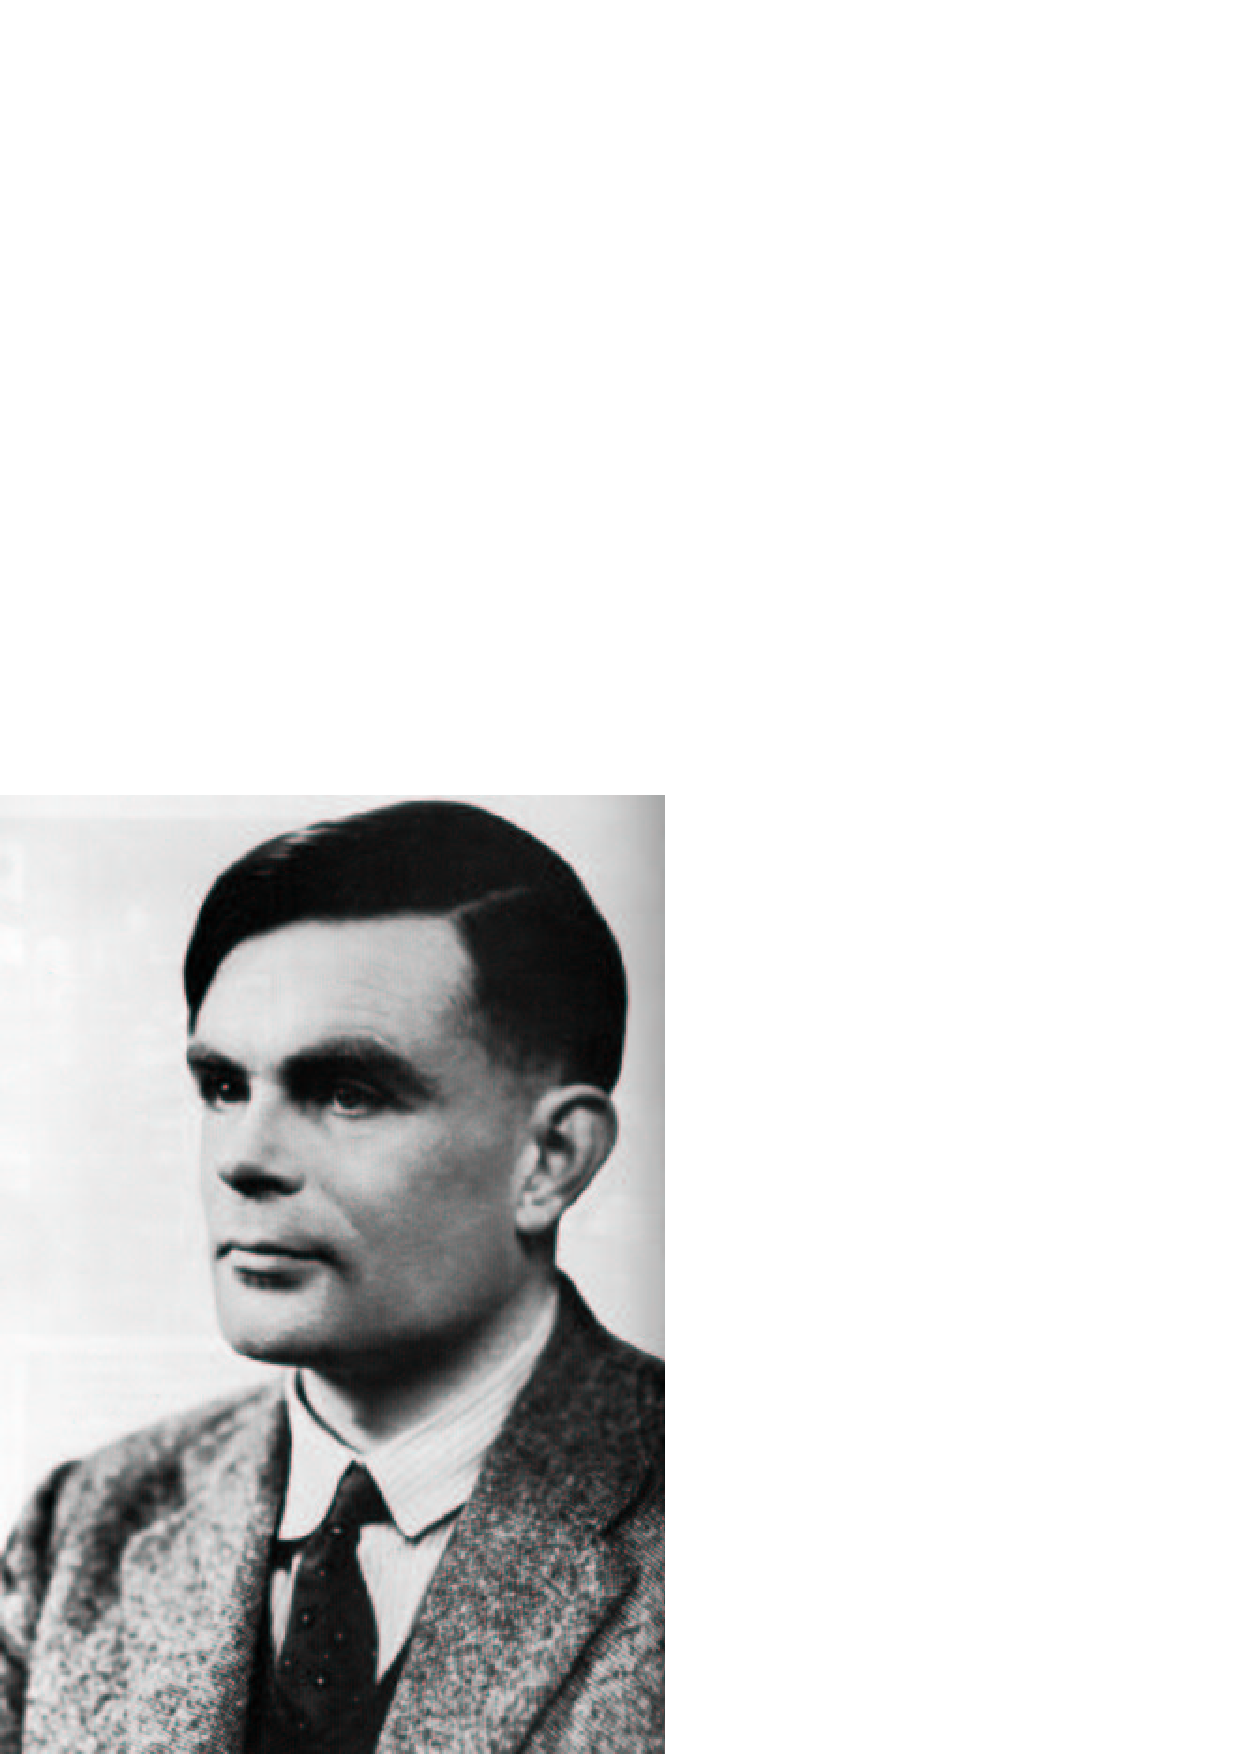
\includegraphics[width=2in]{figures/turing.pdf}}

The man pictured above is Alan Turing, the most important figure in
the history of computer science.  For decades, his fascinating life
story was shrouded by government secrecy, societal taboo, and even his
own deceptions.

At 24 Turing wrote a paper entitled \emph{On Computable Numbers, with an
Application to the Entscheidungsproblem}.  The crux of the paper was an
elegant way to model a computer in mathematical terms.  This was a
breakthrough, because it allowed the tools of mathematics to be brought to
bear on questions of computation.  For example, with his model in hand,
Turing immediately proved that there exist problems that no computer can
solve--- no matter how ingenious the programmer.  Turing's paper is all the
more remarkable because he wrote it in 1936, a full decade before any
electronic computer actually existed.

The word ``Entscheidungsproblem'' in the title refers to one of the 28
mathematical problems posed by David Hilbert in 1900 as challenges to
mathematicians of the 20th century.  Turing knocked that one off in the
same paper.  And perhaps you've heard of the ``\idx{Church-Turing
  thesis}''?  Same paper.  So Turing was obviously a brilliant guy who
generated lots of amazing ideas.  But this lecture is about one of
Turing's less-amazing ideas.  It involved codes.  It involved number
theory.  And it was sort of stupid.

%\subsection{Turing's Code}

Let's look back to the fall of 1937.  Nazi Germany was rearming under
Adolf Hitler, world-shattering war looked imminent, and--- like us--- Alan
Turing was pondering the usefulness of number theory.  He foresaw that
preserving military secrets would be vital in the coming conflict and
proposed a way \emph{to encrypt communications using number theory}.
This is an idea that has ricocheted up to our own time.  Today, number
theory is the basis for numerous public-key cryptosystems, digital
signature schemes, cryptographic hash functions, and digital cash systems.
Every time you buy a book from Amazon, check your grades on WebSIS, or use
a PayPal account, you are relying on number theoretic algorithms.
Furthermore, military funding agencies are among the biggest investors in
cryptographic research.  Sorry \idx{Hardy}!

Soon after devising his code, \idx{Turing} disappeared from public view,
and half a century would pass before the world learned the full story of
where he'd gone and what he did there.  We'll come back to Turing's life
in a little while; for now, let's investigate the code Turing left behind.
The details are uncertain, since he never formally published the idea, so
we'll consider a couple of possibilities.

\subsection{Turing's Code (Version 1.0)}

The first challenge is to translate a text message into an integer so
we can perform mathematical operations on it.  This step is not
intended to make a message harder to read, so the details are not too
important.  Here is one approach: replace each letter of the message
with two digits ($A = 01$, $B = 02$, $C = 03$, etc.) and string all
the digits together to form one huge number.  For example, the message
``victory'' could be translated this way:
%
\begin{center}
\begin{tabular}{ccccccccc}
   &``v &  i &  c &  t & o & r & y'' \\
$\rightarrow$ & 22 & 09 & 03 & 20 & 15 & 18 & 25
\end{tabular}
\end{center}
%
\idx{Turing's code} requires the message to be a prime number, so we may
need to pad the result with a few more digits to make a prime.  In
this case, appending the digits 13 gives the number 2209032015182513,
which is prime.

Now here is how the encryption process works.  In the description
below, $m$ is the unencoded message (which we want to keep secret),
$m^*$ is the encrypted message (which the Nazis may intercept), and
$k$ is the key.

\begin{description}

\item[Beforehand] The sender and receiver agree on a secret key, which
is a large prime $k$.

\item[Encryption] The sender encrypts the message $m$ by computing:
\[
m^* = m \cdot k
\]

\item[Decryption] The receiver decrypts $m^*$ by computing:
\[
\frac{m^*}{k} = \frac{m \cdot k}{k} = m
\]

\end{description}

For example, suppose that the secret key is the prime number $k =
22801763489$ and the message $m$ is ``victory''.  Then the encrypted
message is:
%
\begin{align*}
m^* & = m \cdot k \\
   & = 2209032015182513 \cdot 22801763489 \\
   & = 50369825549820718594667857
\end{align*}

There are a couple of questions that one might naturally ask about Turing's
code.

\begin{enumerate}

\item How can the sender and receiver ensure that $m$ and $k$ are
prime numbers, as required?

The general problem of determining whether a large number is prime or
composite has been studied for centuries, and reasonably good primality
tests were known even in Turing's time.  In 2002, Manindra Agrawal, Neeraj
Kayal, and Nitin Saxena announced a primality test that is guaranteed to
work on a number $n$ in about $(\log n)^{12}$ steps, that is, a number of
steps bounded by a twelfth degree polynomial in the length (in bits) of
the input, $n$.  This definitively places primality testing way below the
problems of exponential difficulty.  Amazingly, the description of their
breakthrough algorithm was only thirteen lines long!

Of course, a twelfth degree polynomial grows pretty fast, so the
Agrawal,\emph{ et al.}\ procedure is of no practical use.  Still, good
ideas have a way of breeding more good ideas, so there's certainly hope
further improvements will lead to a procedure that is useful in practice.
But the truth is, there's no practical need to improve it, since very
efficient \emph{probabilistic} procedures for prime-testing have been
known since the early 1970's.  These procedures have some probability of
giving a wrong answer, but their probability of being wrong is so tiny
that betting on their answers is the best bet you'll ever make.

\item Is Turing's code secure?

The Nazis see only the encrypted message $m^* = m \cdot k$, so
recovering the original message $m$ requires factoring $m^*$.  Despite
immense efforts, no really efficient factoring algorithm has ever been
found.  It appears to be a fundamentally difficult problem, though a
breakthrough someday is not impossible.  In effect, Turing's code puts
to practical use his discovery that there are limits to the power of
computation.  Thus, provided $m$ and $k$ are sufficiently large, the
Nazis seem to be out of luck!

\end{enumerate}

This all sounds promising, but there is a major flaw in Turing's code.

\subsection{Breaking Turing's Code}

Let's consider what happens when the sender transmits a
\emph{second} message using Turing's code and the same key.  This
gives the Nazis two encrypted messages to look at:
%
\[
m_1^* = m_1 \cdot k
\hspace{0.75in} \text{and} \hspace{0.75in}
m_2^* = m_2 \cdot k
\]
%
The greatest common divisor of the two encrypted messages, $m_1^*$ and
$m_2^*$, is the secret key $k$.  And, as we've seen, the $\gcd$ of two
numbers can be computed very efficiently.  So after the second message is
sent, the Nazis can recover the secret key and read \emph{every}
message!

It is difficult to believe a mathematician as brilliant as Turing
could overlook such a glaring problem.  One possible explanation is
that he had a slightly different system in mind, one based on
\emph{modular} arithmetic.

%% Problems %%%%%%%%%%%%%%%%%%%%%%%%%%%%%%%%%%%%%%%%%%%%%%%%%%%%%%%%%%%%%%%%%%%
%\startclassproblems
%\pinput{CP_}


%% Modular Arithmetic %%%%%%%%%%%%%%%%%%%%%%%%%%%%%%%%%%%%%%%%%%%%%%%%%%%%%%%%%
\hyperdef{modular}{arithmetic}{\section{Modular Arithmetic}}
\label{modular_arithmeric_sec}

% Congruence is a weak form of equality.

On page 1 of his masterpiece on number theory, \emph{Disquisitiones
  Arithmeticae}, \idx{Gauss} introduced the notion of
``\idx{congruence}''.  Now, Gauss is another guy who managed to cough up a
half-decent idea every now and then, so let's take a look at this one.
Gauss said that $a$ is \term{congruent} to $b$ \term{modulo} $n$ iff $n
\divides (a - b)$.  This is denoted $a$ \index{$\equiv \pmod{n}$} $b
\pmod{n}$.  For example:
%
\[
29 \equiv 15 \pmod{7}  \quad\text{ because }  7 \divides (29 - 15).
\]

There is a close connection between congruences and remainders:
\begin{lemma}[Congruences and Remainders]
\label{lem:conrem}
\[
a \equiv b \pmod{n} \qiff \rem{a}{n} = \rem{b}{n}.
\]
\end{lemma}

\begin{proof}
By the Division Theorem, there exist unique pairs of integers $q_1, r_1$
and $q_2, r_2$ such that:
%
\begin{align*}
a & = q_1 n + r_1 & \text{where $0 \leq r_1 < n$}, \\
b & = q_2 n + r_2 & \text{where $0 \leq r_2 < n$}.
\end{align*}
%
In these terms, $\rem{a}{n} = r_1$ and $\rem{b}{n} = r_2$.
Subtracting the second equation from the first gives:
%
\begin{align*}
a - b & = (q_1 - q_2) n + (r_1 - r_2)
  & \text{where $-n < r_1 - r_2 < n$}.
\end{align*}
%
Now $a \equiv b \pmod{n}$ if and only if $n$ divides the left side.
This is true if and only if $n$ divides the right side, which holds if
and only if $r_1 - r_2$ is a multiple of $n$.  Given the bounds on
$r_1 - r_2$, this happens precisely when $r_1 = r_2$, which is
equivalent to $\rem{a}{n} = \rem{b}{n}$.
\end{proof}

So we can also see that
\[
29 \equiv 15 \pmod{7} \quad\text{ because } \rem{29}{7} = 1 = \rem{15}{7}.
\]
This formulation explains why the congruence relation has properties like
an equality relation.  Notice that even though (mod 7) appears over on the
right side the $\equiv$ symbol, it is in no sense more strongly associated
with the 15 than the 29.  It would really be clearer to write $29
\equiv_{\mod 7} 15$ for example, but the notation with the modulus at the
end is firmly entrenched and we'll stick to it.

We'll make frequent use of the following immediate Corollary of
Lemma~\ref{lem:conrem}:
\begin{corollary}\label{aran}
\[
a \equiv \rem{a}{n} \pmod{n}
\]
\end{corollary}

Still another way to think about congruence modulo $n$ is that it
\emph{defines a partition of the integers into $n$ sets so that congruent
numbers are all in the same set}.  For example, suppose that we're working
modulo 3.  Then we can partition the integers into 3 sets as follows:
%
\[
\begin{array}{cccccccccc}
\{ & \dots, & -6, & -3, & 0, & 3, & 6, & 9, & \dots & \} \\
\{ & \dots, & -5, & -2, & 1, & 4, & 7, & 10, & \dots & \} \\
\{ & \dots, & -4, & -1, & 2, & 5, & 8, & 11, & \dots & \}
\end{array}
\]
according to whether their remainders on division by 3 are 0, 1, or 2.
The upshot is that when arithmetic is done modulo $n$ there are really
only $n$ different kinds of numbers to worry about, because there are only
$n$ possible remainders.  In this sense, modular arithmetic is a
simplification of ordinary arithmetic and thus is a good reasoning tool.

There are many useful facts about congruences, some of which are listed in
the lemma below.  The overall theme is that \emph{congruences work a lot
like equations}, though there are a couple of exceptions.

\begin{lemma}[Facts About Congruences]  The following  hold for 
$n \geq 1$:
%
\begin{enumerate}
\item $a \equiv a \pmod{n}$
\item $a \equiv b \pmod{n}$ implies $b \equiv a \pmod{n}$
\item $a \equiv b \pmod{n}$ and $b \equiv c \pmod{n}$ implies $a \equiv c \pmod{n}$
\item $a \equiv b \pmod{n}$ implies $a + c \equiv b + c \pmod{n}$
\item $a \equiv b \pmod{n}$ implies $a c \equiv b c \pmod{n}$
\item $a \equiv b \pmod{n}$ and $c \equiv d \pmod{n}$ imply $a + c
\equiv b + d \pmod{n}$
\item $a \equiv b \pmod{n}$ and $c \equiv d \pmod{n}$ imply $a c
\equiv b d \pmod{n}$
\end{enumerate}
\end{lemma}

\begin{proof}
Parts 1.--3.\ follow immediately from Lemma~\ref{lem:conrem}.  Part 4.\
follows immediately from the definition that $a \equiv b \pmod{n}$ iff $n
\divides (a-b)$.  Likewise, part 5.\ follows because if $n \divides (a-b)$
then it divides $(a-b)c = ac - bc$.  To prove part 6., assume
\begin{equation}\label{ab}
a \equiv b \pmod{n}
\end{equation}
and
\begin{equation}\label{cd}
c \equiv d \pmod{n}.
\end{equation}
Then
\begin{align*}
a + c & \equiv b + c \pmod{n} & \text{(by part 4.\ and~\eqref{ab}}),\\
c + b & \equiv d + b \pmod{n} & \text{(by part 4.\ and~\eqref{cd}), so}\\
b + c & \equiv b + d \pmod{n} & \text{and therefore}\\
a + c & \equiv b + d \pmod{n} & \text{(by part 3.)}
\end{align*}
Part 7.\ has a similar proof.
\end{proof}

\iffalse

There is a close connection between modular arithmetic and the
remainder operation, which we looked at last time.  To clarify this
link, let's reconsider the partition of the integers defined by
congruence modulo 3:
%
\[
\begin{array}{cccccccccc}
\{ & \dots, & -6, & -3, & 0, & 3, & 6, & 9, & \dots & \} \\
\{ & \dots, & -5, & -2, & 1, & 4, & 7, & 10, & \dots & \} \\
\{ & \dots, & -4, & -1, & 2, & 5, & 8, & 11, & \dots & \}
\end{array}
\]
%
Notice that two numbers are in the same set if and only if they leave
the same remainder when divided by 3.  The numbers in the first set
all leave a remainder of 0 when divided by 3, the numbers in the
second set leave a remainder of 1, and the numbers in the third leave
a remainder of 2.  Furthermore, notice that each number is in the same
set as its own remainder.  For example, 11 and $\rem{11}{3} = 2$ are
both in the same set.  Let's bundle all this happy goodness into a
lemma.
\fi

%\TBA{put in 'example' environment}

\subsection{\idx{Turing's Code} (Version 2.0)}

In 1940 France had fallen before Hitler's army, and Britain alone stood
against the Nazis in western Europe.  British resistance depended on a
steady flow of supplies brought across the north Atlantic from the United
States by convoys of ships.  These convoys were engaged in a cat-and-mouse
game with German ``U-boats'' ---submarines ---which prowled the Atlantic,
trying to sink supply ships and starve Britain into submission.  The
outcome of this struggle pivoted on a balance of information: could the
Germans locate convoys better than the Allies could locate U-boats or vice
versa?

Germany lost.

But a critical reason behind Germany's loss was made public only in
1974: the British had broken Germany's naval code, Enigma.  Through
much of the war, the Allies were able to route convoys around German
submarines by listening into German communications.  The British
government didn't explain \emph{how} Enigma was broken until 1996.
When the analysis was finally released (by the US), the author was
none other than Alan Turing.  In 1939 he had joined the secret British
codebreaking effort at Bletchley Park.  There, he played a central
role in cracking the German's Enigma code and thus in preventing
Britain from falling into Hitler's hands.

Governments are always tight-lipped about cryptography, but the
half-century of official silence about Turing's role in breaking
Enigma and saving Britain may be related to some disturbing events
after the war.

Let's consider an alternative interpretation of Turing's code.
Perhaps we had the basic idea right (multiply the message by the key),
but erred in using \emph{conventional} arithmetic instead of
\emph{modular} arithmetic.  Maybe this is what Turing meant:
%
\begin{description}

\item[Beforehand] The sender and receiver agree on a large prime $p$,
which may be made public.  (This will be the modulus for all our
arithmetic.)  They also agree on a secret key $k \in \set{1, 2,
\dots, p-1}$.

\item[Encryption] The message $m$ can be any integer in the set
$\set{0, 1, 2, \dots, p-1}$; in particular, the message is no longer
required to be a prime.  The sender encrypts the message $m$ to
produce $m^*$ by computing:
%
\begin{equation}
m^* = \rem{mk}{p} \label{eq:turing-code}
\end{equation}

\item[Decryption] (Uh-oh.)

\end{description}

The decryption step is a problem.  We might hope to decrypt in the
same way as before: by dividing the encrypted message $m^*$ by the key
$k$.  The difficulty is that $m^*$ is the \emph{remainder} when $mk$
is divided by $p$.  So dividing $m^*$ by $k$ might not even give us an
integer!

This decoding difficulty can be overcome with a better understanding
of arithmetic modulo a prime.

%% Problems %%%%%%%%%%%%%%%%%%%%%%%%%%%%%%%%%%%%%%%%%%%%%%%%%%%%%%%%%%%%%%%%%%%
\begin{problems}
\classproblems
\pinput{CP_proving_basic_congruence_properties}
\pinput{CP_multiples_of_9_and_11}
\pinput{CP_13th_roots}
\end{problems}

%% Arithmetic with a Prime Modulus %%%%%%%%%%%%%%%%%%%%%%%%%%%%%%%%%%%%%%%%%%%%
\section{Arithmetic with a Prime Modulus}\label{mod_prime_sec}

\subsection{\idx{Multiplicative Inverses}}
\label{sec:prime}

The \term{multiplicative inverse} of a number $x$ is another number
$x^{-1}$ such that:
%
\[
x \cdot x^{-1} = 1
\]

Generally, multiplicative inverses exist over the real numbers.  For
example, the multiplicative inverse of 3 is $1 / 3$ since:
%
\[
3 \cdot \frac{1}{3} = 1
\]
%
The sole exception is that 0 does not have an inverse.

On the other hand, inverses generally do not exist over the integers.
For example, 7 can not be multiplied by another integer to give 1.

Surprisingly, multiplicative inverses do exist when we're working
\emph{modulo a prime number}.  For example, if we're working modulo
5, then 3 is a multiplicative inverse of 7, since:
%
\[
7 \cdot 3 \equiv 1 \pmod{5}
\]
%
(All numbers congruent to 3 modulo 5 are also multiplicative inverses
of 7; for example, $7 \cdot 8 \equiv 1 \pmod{5}$ as well.)  The only
exception is that numbers congruent to 0 modulo 5 (that is, the
multiples of 5) do not have inverses, much as 0 does not have an
inverse over the real numbers.  Let's prove this.

\begin{lemma}
\label{lem:inverses}
If $p$ is prime and $k$ is not a multiple of $p$, then $k$ has a
multiplicative inverse.
\end{lemma}

\begin{proof}
Since $p$ is prime, it has only two divisors: 1 and $p$.  And since
$k$ is not a multiple of $p$, we must have $\gcd(p, k) = 1$.
Therefore, there is a linear combination of $p$ and $k$ equal to 1:
%
\[
s p + t k = 1
\]
%
Rearranging terms gives:
%
\[
s p = 1 - t k
\]
%
This implies that $p \divides \paren{1 - tk}$ by the definition of divisibility,
and therefore $tk \equiv 1 \pmod{p}$ by the definition of congruence.
Thus, $t$ is a multiplicative inverse of $k$.
\end{proof}

Multiplicative inverses are the key to decryption in Turing's code.
Specifically, we can recover the original message by multiplying the
encoded message by the \emph{inverse} of the key:
\begin{align*}
m^* \cdot k^{-1}
    & = \rem{mk}{p} \cdot k^{-1}
         & \text{(def.~\eqref{eq:turing-code} of $m^*$)}\\
    & \equiv (mk)k^{-1} \pmod{p} & \text{(by Cor.~\ref{aran})}\\
    & \equiv m \pmod{p}.
\end{align*}

This shows that $m^* k^{-1}$ is congruent to the original message $m$.
Since $m$ was in the range $0, 1, \dots, p - 1$, we can recover
it exactly by taking a remainder:
%
\[
m = \rem{m^* k^{-1}}{p}
\]
%
So now we can decrypt!

\subsection{\idx{Cancellation}}

Another sense in which real numbers are nice is that one can cancel
multiplicative terms.  In other words, if we know that $m_1 k = m_2 k$,
then we can cancel the $k$'s and conclude that $m_1 = m_2$, provided $k
\neq 0$.  In general, cancellation is \emph{not} valid in modular
arithmetic.  For example, this congruence is correct:
%
\[
2 \cdot 3 \equiv 4 \cdot 3 \pmod{6}
\]
%
But if we cancel the 3's, we reach a false conclusion:
%
\[
2 \equiv 4 \pmod{6}
\]
%
The fact that multiplicative terms can not be cancelled is the most
significant sense in which congruences differ from ordinary equations.
However, this difference goes away if we're working modulo a
\emph{prime}; then cancellation is valid.

\begin{lemma}
\label{lem:cancel}
Suppose $p$ is a prime and $k$ is not a multiple of $p$.  Then
%
\[
ak \equiv bk \pmod{p}
\hspace{0.5in} \text{implies} \hspace{0.5in}
a \equiv b \pmod{p}
\]
\end{lemma}

\begin{proof}
Multiply both sides of the congruence by $k^{-1}$.
\end{proof}

We can use this lemma to get a bit more insight into how Turing's code
works.  In particular, the encryption operation in Turing's code
\emph{permutes the set of possible messages}.  This is stated more
precisely in the following corollary.

\hyperdef{for}{Fermat}{\begin{corollary}
\label{cor:prime-permutes}
Suppose $p$ is a prime and $k$ is not a multiple of $p$.  Then the
sequence:
\[
\rem{(0 \cdot k)}{p},\quad
\rem{(1 \cdot k)}{p},\quad
\rem{(2 \cdot k)}{p},\quad
 \dots,\quad
\rem{\paren{(p-1) \cdot k}}{p}
\]
is a permutation\footnote{A \term{permutation} of a sequence of elements
is a sequence with the same elements (including repeats) possibly in a
different order.  More formally, if
\[
\vec{e} \eqdef e_1,e_2,\dots,e_n
\]
is a length $n$ sequence, and  $\pi: \set{1,\dots, n} \to \set{1,\dots,
n}$ is a bijection, then
\[
e_{\pi(1)}, e_{\pi(2)},\dots, e_{\pi(n)},
\]
is a \emph{permutation} of $\vec{e}$.} of the sequence:
\[
0,\quad 1,\quad 2,\quad \dots,\quad (p - 1)
\]
This remains true if the first term is deleted from each sequence.
\end{corollary}}

\begin{proof}
The first sequence contains $p$ numbers, which are all in the range
$0$ to $p - 1$ by the definition of remainder.  Furthermore, the
numbers in the first sequence are all different; by
Lemma~\ref{lem:cancel}, $i k \equiv j k \pmod{p}$
if and only if $i \equiv j \pmod{p}$, and no two numbers in the range 0, 1,
\dots, p - 1 are congruent modulo $p$.  Thus, the first sequence must
contain \emph{all} of the numbers from 0 to $p - 1$ in some order.
The claim remains true if the first terms are deleted, because both
sequences begin with 0.
\end{proof}

For example, suppose $p = 5$ and $k = 3$.  Then the sequence:
%
\[
\underbrace{\rem{(0 \cdot 3)}{5}}_{=0},\quad
\underbrace{\rem{(1 \cdot 3)}{5}}_{=3},\quad
\underbrace{\rem{(2 \cdot 3)}{5}}_{=1},\quad
\underbrace{\rem{(3 \cdot 3)}{5}}_{=4},\quad
\underbrace{\rem{(4 \cdot 3)}{5}}_{=2}
\]
%
is a permutation of 0, 1, 2, 3, 4 and the last four terms are a
permutation of 1, 2, 3, 4.  As long as the Nazis don't know the secret key
$k$, they don't know how the set of possible messages are permuted by the
process of encryption and thus can't read encoded messages.

%%%%%%%%%%%%%%%%%%%%%%%%%%%%%%%%%%%%%%%%%%%%%%%%%%%%%%%%%%%%%%%%%%%%%%%%%%%%%%%

\subsection{Fermat's Little Theorem}

A remaining challenge in using Turing's code is that decryption requires
the inverse of the secret key $k$.  An effective way to calculate
$k^{-1}$ follows from the proof of Lemma~\ref{lem:inverses}: $k^{-1} =
\rem{t}{p}$ where $s,t$ are coefficients such that $sp+tk=1$.  Notice that
$t$ is easy to find using the Pulverizer.

An alternative approach, about equally efficient and probably more
memorable, is to rely on Fermat's Little Theorem, which is much easier than his
famous Last Theorem.  \iffalse ---and more useful.\fi


\begin{theorem}[\idx{Fermat's Little Theorem}]\label{fermat_little}
Suppose $p$ is a prime and $k$ is not a multiple of $p$.  Then:
%
\[
k^{p-1} \equiv 1 \pmod{p}
\]
\end{theorem}

\begin{proof}
We reason as follows:
\begin{align*}
1 \cdot 2 \cdots (p-1)
	& = \rem{k}{p} \cdot \rem{2k}{p} \cdots
	\rem{(p-1)k}{p} & \text{(by Cor~\ref{cor:prime-permutes})}\\
	& \equiv k \cdot 2k \cdots (p-1) k \pmod{p}
            & \text{(by Cor~\ref{aran})}\\
	& \equiv (p-1)! \cdot k^{p-1} \pmod{p} & \text{(rearranging terms)}\\
\end{align*}

Now $(p - 1)!$ can not be a multiple of $p$, because the prime
factorizations of $1, 2, \dots, (p - 1)$ contain only primes smaller
than $p$.  Therefore, we can cancel $(p - 1)!$ from the first
expression and the last by Lemma~\ref{lem:cancel}, which proves the
claim.
\end{proof}

Here is how we can find inverses using Fermat's Theorem.  Suppose $p$
is a prime and $k$ is not a multiple of $p$.  Then, by Fermat's
Theorem, we know that:
%
\[
k^{p-2} \cdot k \equiv 1 \pmod{p}
\]
%
Therefore, $k^{p-2}$ must be a multiplicative inverse of $k$.  For
example, suppose that we want the multiplicative inverse of 6 modulo
17.  Then we need to compute $\rem{6^{15}}{17}$, which we can do by
successive squaring.  All the congruences below hold modulo 17.
%
\begin{align*}
6^2 & \equiv 36 \equiv 2 \\
6^4 & \equiv (6^2)^2 \equiv 2^2 \equiv 4 \\
6^8 & \equiv (6^4)^2 \equiv 4^2 \equiv 16 \\
6^{15} & \equiv 6^8 \cdot 6^4 \cdot 6^2 \cdot 6
       \equiv 16 \cdot 4 \cdot 2 \cdot 6
       \equiv 3
\end{align*}
%
Therefore, $\rem{6^{15}}{17} = 3$.  Sure enough, 3 is the multiplicative
inverse of 6 modulo 17, since:
%
\[
3 \cdot 6 \equiv 1 \pmod{17}
\]

In general, if we were working modulo a prime $p$, finding a
multiplicative inverse by trying every value between 1 and $p - 1$
would require about $p$ operations.  However, the approach above
requires only about $\log p$ operations, which is far better when $p$
is large.

\subsection{Breaking \idx{Turing's Code} ---Again}

The Germans didn't bother to encrypt their weather reports with the
highly-secure Enigma system.  After all, so what if the Allies learned
that there was rain off the south coast of Iceland?  But, amazingly, this
practice provided the British with a critical edge in the Atlantic naval
battle during 1941.

The problem was that some of those weather reports had originally been
transmitted from U-boats out in the Atlantic.  Thus, the British
obtained both unencrypted reports and the same reports encrypted with
Enigma.  By comparing the two, the British were able to determine
which key the Germans were using that day and could read all other
Enigma-encoded traffic.  Today, this would be called a
\term{known-plaintext attack}.

Let's see how a known-plaintext attack would work against Turing's
code.  Suppose that the Nazis know both $m$ and $m^*$ where:
%
\[
m^* \equiv mk \pmod{p}
\]
%
Now they can compute:
%
\begin{align*}
m^{p-2} \cdot m^*
  & = m^{p-2} \cdot \rem{mk}{p}
                & \text{(def.~\eqref{eq:turing-code} of $m^*$)}\\
  & \equiv m^{p-2} \cdot mk \pmod{p} & \text{(by Cor~\ref{aran})}\\
  & \equiv m^{p-1} \cdot k \pmod{p}\\ % & \text{(simplification)}\\
  & \equiv k \pmod{p} & \text{(Fermat's Theorem)}
\end{align*}
%
Now the Nazis have the secret key $k$ and can decrypt any message!

This is a huge vulnerability, so Turing's code has no practical value.
Fortunately, Turing got better at cryptography after devising this
code; his subsequent cracking of Enigma surely saved thousands of
lives, if not the whole of Britain.

%  I could insert a bit about public-key cryptography here as introduction to
%  the recitation.

\subsection{Turing Postscript}

A few years after the war, Turing's home was robbed.  Detectives soon
determined that a former homosexual lover of Turing's had conspired in the
robbery.  So they arrested him ---that is, they arrested Alan Turing
---because homosexuality was a British crime punishable by up to two years
in prison at that time.  Turing was sentenced to a humiliating hormonal
``treatment'' for his homosexuality: he was given estrogen injections.  He
began to develop breasts.

Three years later, Alan \idx{Turing}, the founder of computer science, was
dead.  His mother explained what happened in a biography of her own
son.  Despite her repeated warnings, Turing carried out chemistry
experiments in his own home.  Apparently, her worst fear was realized:
by working with potassium cyanide while eating an apple, he poisoned
himself.

However, Turing remained a puzzle to the very end.  His mother was a
devoutly religious woman who considered suicide a sin.  And, other
biographers have pointed out, Turing had previously discussed
committing suicide by eating a poisoned apple.  Evidently, Alan
Turing, who founded computer science and saved his country, took his
own life in the end, and in just such a way that his mother could
believe it was an accident.

Turing's last project before he disappeared from public view in 1939
involved the construction of an elaborate mechanical device to test a
mathematical conjecture called the Riemann Hypothesis.  This conjecture
first appeared in a sketchy paper by Berhard Riemann in 1859 and is now
one of the most famous unsolved problem in mathematics.

\floatingtextbox{
\textboxtitle{The \idx{Riemann Hypothesis}}

The formula for the sum of an infinite geometric series says:
\[
1 + x + x^2 + x^3 + \cdots = \frac{1}{1-x}
\]
Substituting $x = \frac{1}{2^s}$, $x = \frac{1}{3^s}$, 
$x = \frac{1}{5^s}$, and so on for each prime
number gives a sequence of equations:
%
\begin{align*}
1 + \frac{1}{2^s} + \frac{1}{2^{2s}} + \frac{1}{2^{3s}} + \cdots
    & = \frac{1}{1 - 1 / 2^s} \\
1 + \frac{1}{3^s} + \frac{1}{3^{2s}} + \frac{1}{3^{3s}} + \cdots
    & = \frac{1}{1 - 1 / 3^s} \\
1 + \frac{1}{5^s} + \frac{1}{5^{2s}} + \frac{1}{5^{3s}} + \cdots
    & = \frac{1}{1 - 1 / 5^s} \\
    & \text{etc.}
\end{align*}
%
Multiplying together all the left sides and all the right sides gives:
%
\[
\sum_{n=1}^{\infty} \frac{1}{n^s} = \prod_{p \in \text{primes}} \paren{\frac{1}{1 - 1 / p^s}}
\]
%
The sum on the left is obtained by multiplying out all the infinite
series and applying the Fundamental Theorem of Arithmetic.  For
example, the term $1 / 300^s$ in the sum is obtained by multiplying $1
/ 2^{2s}$ from the first equation by $1 / 3^s$ in the second and $1 /
5^{2s}$ in the third.  Riemann noted that every prime appears in the
expression on the right.  So he proposed to learn about the primes by
studying the equivalent, but simpler expression on the left.  In
particular, he regarded $s$ as a complex number and the left side as a
function, $\zeta(s)$.  Riemann found that the distribution of primes
is related to values of $s$ for which $\zeta(s) = 0$, which led to his
famous conjecture:
\begin{quote}
  \term{The Riemann Hypothesis}: Every nontrivial zero of the zeta
  function $\zeta(s)$ lies on the line $s = 1/2 + c i$ in the complex
  plane.
\end{quote}

Researchers continue to work intensely to settle this conjecture, as they
have for over a century.  A proof would immediately imply, among other
things, a strong form of the \idx{Prime Number Theorem} ---and earn the
prover a \$1 million prize!  (We're not sure what the cash would be for a
counter-example, but the discoverer would be wildly applauded by
mathematicians everywhere.)}

%% Problems %%%%%%%%%%%%%%%%%%%%%%%%%%%%%%%%%%%%%%%%%%%%%%%%%%%%%%%%%%%%%%%%%%%
\begin{problems}
\classproblems
\pinput{CP_nonparallel_lines}
\pinput{CP_Sk_equiv_-1_mod_p}

\homeworkproblems
\pinput{PS_calculating_inverses}
\end{problems}

%% Arithmetic with an Arbitrary Modulus %%%%%%%%%%%%%%%%%%%%%%%%%%%%%%%%%%%%%%%
\hyperdef{mod}{n}{\section{Arithmetic with an Arbitrary
    Modulus}}\label{arithmetic_modn_sec}

Turing's code did not work as he hoped.  However, his essential
idea--- using number theory as the basis for cryptography--- succeeded
spectacularly in the decades after his death.

In 1977, Ronald \idx{Rivest}, Adi \idx{Shamir}, and Leonard \idx{Adleman}
at MIT proposed a highly secure cryptosystem (called \textbf{\idx{RSA}})
based on number theory.  Despite decades of attack, no significant
weakness has been found.  Moreover, RSA has a major advantage over
traditional codes: the sender and receiver of an encrypted message need
not meet beforehand to agree on a secret key.  Rather, the receiver has
both a \term{secret key}, which she guards closely, and a \term{public
  key}, which she distributes as widely as possible.  To send her a
message, one encrypts using her widely-distributed public key.  Then she
decrypts the message using her closely-held private key.  The use of such
a \term{public key cryptography} system allows you and Amazon, for
example, to engage in a secure transaction without meeting up beforehand
in a dark alley to exchange a key.

Interestingly, RSA does not operate modulo a prime, as Turing's scheme
may have, but rather modulo the product of \emph{two} large primes.
Thus, we'll need to know a bit about how arithmetic works modulo a
composite number in order to understand RSA.  Arithmetic modulo an
arbitrary positive integer is really only a little more painful than
working modulo a prime, in the same sense that a doctor says ``This is
only going to hurt a little'' before he jams a big needle in your arm.

\subsection{Relative Primality and Phi}

First, we need a new definition.  Integers $a$ and $b$ are
\term{relatively prime} iff $\gcd(a, b) = 1$.  For example, 8 and 15
are relatively prime, since $\gcd(8, 15) = 1$.  Note that every
integer is relatively prime to a genuine prime number $p$, except for
multiples of $p$.

We'll also need a certain function that is defined using relative
primality.  Let $n$ be a positive integer.  Then $\phi(n)$ denotes the
number of integers in $\set{1, 2, \dots, n - 1}$ that are relatively prime
to $n$.  For example, $\phi(7) = 6$, since 1, 2, 3, 4, 5, and 6 are all
relatively prime to 7.  Similarly, $\phi(12) = 4$, since only 1, 5, 7, and
11 are relatively prime to 12.  If you know the prime factorization of
$n$, then computing $\phi(n)$ is a piece of cake, thanks to the following
theorem.  The function $\phi$ is known as \term{Euler's $\phi$ function};
it's also called Euler's \emph{\idx{totient}} function.

\begin{theorem}
\label{th:phi}
The function $\phi$ obeys the following relationships:
\begin{enumerate}
\item[(a)] If $a$ and $b$ are relatively prime, then $\phi(ab) = \phi(a)\phi(b)$.
\item[(b)] If $p$ is a prime, then $\phi(p^k) = p^k - p^{k-1}$ for $k \geq 1$.
\end{enumerate}
\end{theorem}

Here's an example of using Theorem~\ref{th:phi} to compute $\phi(300)$:
%
\begin{align*}
\phi(300)
    & = \phi(2^2 \cdot 3 \cdot 5^2)\\
    & = \phi(2^2) \cdot \phi(3) \cdot \phi(5^2)
            & \text{(by Theorem~\ref{th:phi}.(a))}\\
    & = (2^2 - 2^1) (3^1 - 3^0) (5^2 - 5^1) 
            & \text{(by Theorem~\ref{th:phi}.(b))}\\
    & = 80.
\end{align*}
\iffalse
We factor 300 in the first step, use part (1) of Theorem~\ref{th:phi}
twice in the second step, use part (2) in the third step, and then
simplify.
\fi

The proof of Theorem~\ref{th:phi}.(a) requires a few more properties of
modular arithmetic worked out in the next section (see
Problem~\ref{PS_Euler_function_multiplicativity}).  We'll also give
another a proof in a few weeks based on rules for counting things.

To prove Theorem~\ref{th:phi}.(b), notice that the numbers in the interval
from 0 to $p^{k}-1$ that are divisible by $p$ are all those of the form
$mp$.  For $mp$ to be in the interval, $m$ can take any value from 0 to
$p^{k-1}-1$ and no others, so there are exactly $p^{k-1}$ numbers in the
interval that are divisible by $p$.  Now $\phi(p^{k})$ equals the number
of remaining elements in the interval, namely, $p^k -p^{k-1}$.


\subsection{Generalizing to an Arbitrary Modulus}

Let's generalize what we know about arithmetic modulo a prime.  Now,
instead of working modulo a prime $p$, we'll work modulo an arbitrary
positive integer $n$.  The basic theme is that arithmetic modulo $n$ may
be complicated, but the integers {\em relatively prime} to $n$ remain
fairly well-behaved.  For example, the proof of Lemma~\ref{lem:inverses}
of an inverse for $k$ modulo $p$ extends to an inverse for $k$ relatively
prime to $n$:

\begin{lemma}
\label{lem:inverse-arb}
Let $n$ be a positive integer.  If $k$ is relatively prime to $n$,
then there exists an integer $k^{-1}$ such that:
%
\[
k \cdot k^{-1} \equiv 1 \pmod{n}
\]
\end{lemma}


\iffalse
\begin{proof}
There exist integers $s$ and $t$ such that $s k + t n = \gcd(k, n) =
1$ by Theorem~\ref{th:gcd}.  Rearranging terms gives $tn = 1 - sk$,
which implies that $n \divides 1 - sk$ and $sk \equiv 1 \pmod{n}$.  Define
$k^{-1}$ to be $s$.
\end{proof}
\fi

As a consequence of this lemma, we can cancel a multiplicative term
from both sides of a congruence if that term is relatively prime to
the modulus:

\begin{corollary}
\label{cor:cancellation-arb}
Suppose $n$ is a positive integer and $k$ is relatively prime to $n$.
If
%
\[
a k \equiv b k \pmod{n}
\]
%
then
%
\[
a \equiv b \pmod{n}
\]
\end{corollary}

This holds because we can multiply both sides of the first congruence
by $k^{-1}$ and simplify to obtain the second.

\subsection{Euler's Theorem}

\idx{RSA} essentially relies on \idx{Euler's Theorem}, a generalization of
Fermat's Theorem to an arbitrary modulus.  The proof is much like the
proof of Fermat's Theorem, except that we focus on integers relatively
prime to the modulus.  Let's start with a lemma.

\begin{lemma}
\label{lem:permutes-arb}
Suppose $n$ is a positive integer and $k$ is relatively prime to $n$.
Let $k_1, \dots, k_r$ denote all the integers relatively prime to $n$
in the range $0 \leq k_i < n$.  Then the sequence:
%
\[
\rem{k_1 \cdot k}{n},\quad
\rem{k_2 \cdot k}{n},\quad
\rem{k_3 \cdot k}{n},\quad
\quad \dots\quad,
\rem{k_r \cdot k}{n}
\]
%
is a permutation of the sequence:
%
\[
k_1,\quad k_2,\quad \dots\quad, k_r.
\]
\end{lemma}

\begin{proof}
We will show that the numbers in the first sequence are all distinct
and all appear in the second sequence.  Since the two sequences have
the same length, the first must be a permutation of the second.

First, we show that the numbers in the first sequence are all
distinct.  Suppose that $\rem{k_i k}{n} = \rem{k_j k}{n}$.  This is
equivalent to $k_i k \equiv k_j k \pmod{n}$, which implies $k_i \equiv
k_j \pmod{n}$ by Corollary~\ref{cor:cancellation-arb}.  This, in turn,
means that $k_i = k_j$ since both are between 1 and $n-1$.  Thus, a
term in the first sequence is not equal to any other term.

Next, we show that each number in the first sequence appears in the
second.  By assumption, $\gcd(k_i, n) = 1$ and $\gcd(k, n) = 1$, which
means that
%
\begin{align*}
\gcd(n, \rem{k_i k}{n}) & = \gcd(k_i k, n)
            & \text{(by Lemma~\ref{lem:gcd}.\ref{gcd5})}\\
      & = 1 & \text{(by Lemma~\ref{lem:gcd}.\ref{gcd3})}.
\end{align*}
%
So $\rem{k_i k}{n}$ is relatively prime to $n$ and is in the range from 0
to $n - 1$ by the definition of remainder.  The second sequence is defined
to consist of all such integers.
\end{proof}

We can now prove Euler's Theorem:

\begin{theorem}[\idx{Euler's Theorem}]
Suppose $n$ is a positive integer and $k$ is relatively prime to $n$.
Then
\begin{eqnarray*}
k^{\phi(n)} \equiv 1 \pmod{n}
\end{eqnarray*}
\end{theorem}

\begin{proof}
Let $k_1, \dots, k_r$ denote all integers relatively prime to $n$
such that $0 \leq k_i < n$.  Then $r = \phi(n)$, by the definition of
the function $\phi$.  Now we can reason as follows:
%
\begin{align*}
\lefteqn{k_1 \cdot k_2 \cdots k_r} \hspace{0.25in} \\
& =
\rem{k_1 \cdot k}{n} \cdot 
\rem{k_2 \cdot k}{n} \cdots 
\rem{k_r \cdot k}{n} & \text{(by Lemma~\ref{lem:permutes-arb})}
\\
& \equiv 
(k_1 \cdot k) \cdot 
(k_2 \cdot k) \cdot 
\cdots 
(k_r \cdot k) \pmod{n} & \text{(by Cor~\ref{aran})}
\\
& \equiv  
(k_1 \cdot k_2 \cdots k_r) \cdot k^r \pmod{n} & \text{(rearranging terms)}
\end{align*}

Lemma~\ref{lem:gcd}.\ref{gcd3}.\ implies that $k_1 \cdot k_2
\cdots k_r$ is prime relative to $n$.  Therefore, we can cancel this
product from the first expression and the last by
Corollary~\ref{cor:cancellation-arb}.  This proves the claim.
\end{proof}

We can find multiplicative inverses using Euler's theorem as we did
with Fermat's theorem: if $k$ is relatively prime to $n$, then
$k^{\phi(n) - 1}$ is a multiplicative inverse of $k$ modulo $n$.
However, this approach requires computing $\phi(n)$.  Our best method
for doing so requires factoring $n$, which can be quite difficult in
general.  Fortunately, when we know how to factor $n$, we can
use Theorem~\ref{th:phi} to compute $\phi(n)$ efficiently!


\subsection{RSA}
Finally, we are ready to see how the \term{RSA public key encryption
  scheme} works:
\begin{center}
RSA Public Key Encryption
\fbox{
\begin{minipage}[t]{5in}
\vspace{0.1cm}
\begin{description}

\item[Beforehand] The receiver creates a public key and a secret key
as follows.

\begin{enumerate}

\item Generate two distinct primes, $p$ and $q$.

\item Let $n = pq$.

\item Select an integer $e$ such that $\gcd(e, (p-1)(q-1)) = 1$.\\ The
{\em public key} is the pair $(e, n)$.  This should be distributed
widely.

\item Compute $d$ such that $de \equiv 1 \pmod{(p-1)(q-1)}$.\\ The
{\em secret key} is the pair $(d, n)$.  This should be kept hidden!

\end{enumerate}

\item[Encoding] The sender encrypts message $m$ to produce $m^\prime$ using
the public key:

\[
m' = \rem{m^e}{n}.
\]

\item[Decoding] The receiver decrypts message $m'$ back to message $m$
using the secret key:
\[
m = \rem{(m')^d}{n}.
\]

\end{description}

%We'll explain in class why this way of Decoding works!

\vspace{0.1cm}
\end{minipage}
}
\end{center}

%% Problems %%%%%%%%%%%%%%%%%%%%%%%%%%%%%%%%%%%%%%%%%%%%%%%%%%%%%%%%%%%%%%%%%%%
\begin{problems}
%\examproblems

\practiceproblems
\pinput{MQ_modular_arithmetic}
\pinput{MQ_inverse_by_pulverizer}

\classproblems
\pinput{CP_RSA_between_tables}
\pinput{CP_RSA_proving_correctness}

\homeworkproblems
\pinput{PS_Euler_theorem_calculation}
\pinput{PS_Euler_function_multiplicativity}
\end{problems}

\iffalse
%% Conclusion %%%%%%%%%%%%%%%%%%%%%%%%%%%%%%%%%%%%%%%%%%%%%%%%%%%%%%%%%%%%%%%%%
\section{Conclusion}

\TBA{add some sort of conclusion here...  maybe put the RSA algorithm
here and use that as a wrap up since it is what the entire chapter 
builds up to.}

\clearpage
\fi

\endinput
  %thru RSA 

\part{Mathematical Data Types}

\documentclass[twoside,11pt]{article}
\usepackage{light}
\usepackage{graphicx}

\newcommand{\QAND}{\wedge}
\newcommand{\QOR}{\vee}
\newcommand{\QIMP}{\,\, \Rightarrow \,\,}
\newcommand{\QIMPLIES}{\,\, \Rightarrow \,\,}
\newcommand{\diredge}[2]{#1 \to #2}

\begin{document}

\generic{Injections, Surjections, and Bijections}{November 8, 2016}

\subsection*{Arrow properties on a binary relation $R: A \rightarrow B$}
\begin{description}
\item[A function]

$R$ is a \term{function} when it has $[ \leq$ 1 arrow \textbf{out}$]$ property. In terms of a bipartite graph $G$ for the relation, every node on the left is incident to at most one edge.

\item[Surjective]

$R$ is \term{surjective} when it has the  $[ \geq$ 1 arrow \textbf{in}$]$ property.
That is, every point in the righthand, codomain column has at least one arrow pointing to it or in terms of a bipartite graph, $every$ node on the right is incident to at least one edge.

\item[Total]

$R$ is \term{total} when it has $[ \geq$ 1 arrow \textbf{out}$]$ property. $Every$ node on the left is incident to $at$ $least$ one edge.

\item[Injective]

$R$ is \term{injective} when it has $[ \leq$ 1 arrow \textbf{in}$]$ property. That is, every element of the codomain is mapped to by $at\text{ }most$ one element of the domain and $every$ node on the right is incident to at most one edge.

\item[Bijective]

$R$ is \term{bijective} when it has both the [= 1 arrow \textbf{out}] and the [= 1 arrow \textbf{in}] property.
\item[Surjection]
A surjective function is a \term{surjection}
\item[Injection]
An injective function is an \term{injection}.
\item[Bijection]
An injective surjective function is a \term{bijection}
\end{description}
\includegraphics{
\end{document}
    % math data types: sets, functions, sequences
                  %binary relations, mapping lemma, 
                  %TBA: boolean matrices, properties: symmetry, reflexive,...  *Albert

%\chapter{First-Order Logic}\label{logic_chap}

\newcommand{\solves}{\text{Solves}}
\newcommand{\probs}{\text{Probs}}
\newcommand{\even}{\text{Evens}}
\newcommand{\primes}{\text{Primes}}

\section{Quantifiers}

There are a couple of assertions commonly made about a predicate: that it
is \emph{sometimes} true and that it is \emph{always} true.  For
example, the predicate
%
\[
\text{``$x^2 \geq 0$''}
\]
%
is always true when $x$ is a real number.  On the other hand, the
predicate
%
\[
\text{``$5x^2 - 7 = 0$''}
\]
%
is only sometimes true; specifically, when $x = \pm \sqrt{7/5}$.

There are several ways to express the notions of ``always true'' and
``sometimes true'' in English.  The table below gives some general
formats on the left and specific examples using those formats on the
right.  You can expect to see such phrases hundreds of times in
mathematical writing!
%
\begin{center}
\begin{tabular}{ll}
\multicolumn{2}{c}{\textbf{Always True}} \\[1ex]
For all $n$, $P(n)$ is true. & For all $x \in \reals$, $x^2 \geq 0$. \\
$P(n)$ is true for every $n$. & $x^2 \geq 0$ for every $x \in \reals$. \\[2ex]
\multicolumn{2}{c}{\textbf{Sometimes True}} \\[1ex]
There exists an $n$ such that $P(n)$ is true. & There exists an $x \in \reals$ such that $5x^2 - 7 = 0$.\\
$P(n)$ is true for some $n$. & $5x^2 - 7 = 0$ for some $x \in \reals$.\\
$P(n)$ is true for at least one $n$. & $5x^2-7=0$ for at least one $x \in \reals$.
\end{tabular}
\end{center}

All these sentences quantify how often the predicate is true.
Specifically, an assertion that a predicate is always true is called a
\term{universal} quantification, and an assertion that a predicate is
sometimes true is an \term{existential} quantification.  Sometimes the
English sentences are unclear with respect to quantification:
%
\begin{center}
  ``If you can solve any problem we come up with, then you get an \emph{A}
  for the course.''
\end{center}
%
The phrase ``you can solve any problem we can come up with'' could
reasonably be interpreted as either a universal or existential
quantification:
%
\begin{quote}
``you can solve \emph{every} problem we come up with,''
\end{quote}
or maybe
\begin{quote}
``you can solve \emph{at least one} problem we come up with.''
\end{quote}
%
In any case, notice that this quantified phrase appears inside a
larger if-then statement.  This is quite normal; quantified statements
are themselves propositions and can be combined with and, or, implies,
etc., just like any other proposition.

\subsection{More Cryptic Notation}

There are symbols to represent universal and existential
quantification, just as there are symbols for ``and'' ($\wedge$),
``implies'' ($\implies$), and so forth.  In particular, to say that a
predicate, $P$, is true for all values of $x$ in some set, $D$, one
writes:
%
\[
\forall x \in D.\; P(x)
\]
%
The symbol $\forall$ is read ``for all'', so this whole expression is
read ``for all $x$ in $D$, $P(x)$ is true''.  To say that a predicate
$P(x)$ is true for at least one value of $x$ in $D$, one writes:
%
\[
\exists x \in D.\; P(x)
\]
%
The backward-E, \term{$\exists$}, is read ``there exists''.  So this
expression would be read, ``There exists an $x$ in $D$ such that $P(x)$ is
true.''  The symbols $\forall$ and $\exists$ are always followed by a
variable ---usually with an indication of the set the variable ranges over
---and then a predicate, as in the two examples above.

As an example, let $\probs$ be the set of problems we come up with,
$\solves(x)$ be the predicate ``You can solve problem $x$'', and $G$ be
the proposition, ``You get an \emph{A} for the course.''  Then the two
different interpretations of
%
\begin{quote}
  ``If you can solve any problem we come up with, then you get an \emph{A}
  for the course.''
\end{quote}
%
can be written as follows:
%
\[
(\forall x \in \probs.\; \solves(x)) \QIMP G,
\]
or maybe
\[
(\exists x \in \probs.\; \solves(x)) \QIMP G.
\]

\subsection{Mixing Quantifiers}

Many mathematical statements involve several quantifiers.  For
example, \term{Goldbach's Conjecture} states:
%
\begin{center}
``Every even integer greater than 2 is the sum of two primes.''
\end{center}
%
Let's write this more verbosely to make the use of quantification
clearer:
%
\begin{quote}
For every even integer $n$ greater than 2,
there exist primes $p$ and $q$ such that $n = p + q$.
\end{quote}
%
Let $\even$ be the set of even integers greater than 2, and let $\primes$ be the
set of primes.  Then we can write Goldbach's Conjecture in logic
notation as follows:
%
\[
\underbrace{\forall n \in \even}_{\substack
    {\text{for every even} \\
     \text{integer $n > 2$}}}
\
\underbrace{\exists p \in \primes\ \exists q \in \primes.}_{\substack
    {\text{there exist primes} \\
     \text{$p$ and $q$ such that}}}
\ n = p + q.
\]

\subsection{Order of Quantifiers}

Swapping the order of different kinds of quantifiers (existential or
universal) usually changes the meaning of a proposition.  For example,
let's return to one of our initial, confusing statements:
\begin{center}
``Every American has a dream.''
\end{center}

This sentence is ambiguous because the order of quantifiers is
unclear.  Let $A$ be the set of Americans, let $D$ be the set of
dreams, and define the predicate $H(a, d)$ to be ``American $a$ has
dream $d$.''.  Now the sentence could mean there is a single dream
that every American shares:
\[
\exists\, d \in D\; \forall a \in A.\; H(a, d)
\]
For example, it might be that every American shares the dream of owning
their own home.

Or it could mean that every American has a personal dream:
\[
\forall a \in A\; \exists\, d \in D.\; H(a, d)
\]
For example, some Americans may dream of a peaceful retirement, while
others dream of continuing practicing their profession as long as they
live, and still others may dream of being so rich they needn't think at
all about work.

Swapping quantifiers in \idx{Goldbach's Conjecture} creates a patently false
statement that every even number $\geq 2$ is the sum of \emph{the same}
two primes:
\[
\underbrace{\exists\, p \in \primes\ \exists\, q \in \primes}_{\substack
    {\text{there exist primes} \\
     \text{$p$ and $q$ such that}}}
\
\underbrace{\forall n \in \even.}_{\substack
    {\text{for every even} \\
     \text{integer $n > 2$}}}
\ n = p + q.
\]

\subsubsection{Variables over One Domain}
When all the variables in a formula are understood to take values from the
same nonempty set, $D$, it's conventional to omit mention of $D$.  For
example, instead of $\forall x \in D\; \exists y \in D.\; Q(x,y)$ we'd
write $\forall x \exists y.\; Q(x,y)$.  The unnamed nonempty set that $x$
and $y$ range over is called the \term{domain of discourse}, or just plain
\term{domain}, of the formula.

It's easy to arrange for all the variables to range over one domain.  For
example, \idx{Goldbach's Conjecture} could be expressed with all variables
ranging over the domain $\naturals$ as
\[
\forall n.\; n \in \even \QIMP (\exists\, p \exists\, q.\; p \in \primes \land
q \in \primes \land n = p + q).
\]

\subsection{Negating Quantifiers}

There is a simple relationship between the two kinds of quantifiers.  The
following two sentences mean the same thing:
%
\begin{quote}

It is not the case that everyone likes to snowboard.

There exists someone who does not like to snowboard.

\end{quote}
%
In terms of logic notation, this follows from a general property of
predicate formulas:
%
\[
\QNOT \forall x.\; P(x)
\hspace{0.1in} \text{is equivalent to} \hspace{0.1in}
\exists x.\; \QNOT P(x).
\]
%
Similarly, these sentences mean the same thing:
%
\begin{quote}
There does not exist anyone who likes skiing over magma.

Everyone dislikes skiing over magma.
\end{quote}
%
We can express the equivalence in logic notation this way:
%
\begin{equation}\label{nE}
(\QNOT \exists x.\; P(x))  \QIFF  \forall x.\; \QNOT P(x).
\end{equation}
%
The general principle is that \emph{moving a ``not'' across a
quantifier changes the kind of quantifier.}

\iffalse Logicians have worked very hard to define strict rules for the
use of logic notation so that ideas can be expressed with absolute rigor.
It's all quite charming and clever.  However, the sad irony is that
applied mathematicans usually use their beloved notation as a crude
shorthand, breaking the rules and abusing the notation willy-nilly ---sort
of like pounding nails with fine china.  \fi

\subsection{Validity}

A propositional formula is called \term{valid} when it evaluates to \true\
no matter what truth values are assigned to the individual propositional
variables.  For example, the propositional version of the \idx{Distributive Law}
is that $P \QAND (Q \QOR R)$ is equivalent to $(P \QAND Q) \QOR (P \QAND
R)$.  This is the same as saying that
\[
[P \QAND (Q \QOR R)] \QIFF [(P \QAND Q) \QOR (P \QAND R)]
\]
is valid.

The same idea extends to predicate formulas, but to be valid, a
formula now must evaluate to true no matter what values its variables
may take over any unspecified domain, and no matter what
interpretation a predicate variable may be given.  For example, we
already observed that the rule for negating a quantifier is captured
by the valid assertion~\eqref{nE}.

Another useful example of a valid assertion is
\begin{equation}\label{eaimpliesae}
\exists x \forall y.\; P(x,y) \QIMP \forall y \exists x.\; P(x,y).
\end{equation}

Here's an explanation why this is valid:

\begin{quote}
Let $D$ be the domain for the variables and $P_0$ be some
\idx{binary predicate}\footnote{That is, a predicate that depends on two variables.}
on $D$.  We need to show that if
\begin{equation}\label{exayp0}
\exists x \in D\; \forall y \in D.\; P_0(x,y)
\end{equation}
holds under this interpretation, then so does
\begin{equation}\label{ayexp0}
\forall y \in D\; \exists x \in D.\; P_0(x,y).
\end{equation}
So suppose~\eqref{exayp0} is true.  Then by definition of $\exists$, this
means that some element $d_0 \in D$ has the property that
\[
\forall y \in D.\, P_0(d_0, y).
\]
By definition of $\forall$, this means that
\[
P_0(d_0,d)
\]
is true for all $d \in D$.  So given any $d \in D$, there is an element in
$D$, namely, $d_0$, such that $P_0(d_0,d)$ is true.  But that's exactly
what~\eqref{ayexp0} means, so we've proved that~\eqref{ayexp0} holds under
this interpretation, as required.
\end{quote}

We hope this is helpful as an explanation, but we don't really want to
call it a ``proof.''  The problem is that with something as basic
as~\eqref{eaimpliesae}, it's hard to see what more elementary axioms are
ok to use in proving it.  What the explanation above did was translate the
logical formula~\eqref{eaimpliesae} into English and then appeal to the
meaning, in English, of ``for all'' and ``there exists'' as justification.
So this wasn't a proof, just an explanation that once you understand
what~\eqref{eaimpliesae} means, it becomes obvious.

In contrast to~\eqref{eaimpliesae}, the formula
\begin{equation}\label{aenotimplyea}
\forall y \exists x.\; P(x,y) \QIMP \exists x \forall y.\; P(x,y).
\end{equation}
is \emph{not} valid.  We can prove this just by describing an
interpretation where the hypothesis, $\forall y \exists x.\; P(x,y)$, is
true but the conclusion, $\exists x \forall y.\; P(x,y)$, is not true.
For example, let the domain be the integers and $P(x,y)$ mean $x > y$.
Then the hypothesis would be true because, given a value, $n$, for $y$ we
could choose the value of $x$ to be $n+1$, for example.  But under this
interpretation the conclusion asserts that there is an integer that is
bigger than all integers, which is certainly false.  An interpretation
like this which falsifies an assertion is called a \term{counter model} to
the assertion.

\begin{problems}
%\practiceproblems
%\pinput{}
\classproblems
\pinput{CP_logic_news_network}
\pinput{CP_assertions_about_binary_strings}
\pinput{CP_domain_of_discourse}
\pinput{CP_counter_model}
\homeworkproblems
\pinput{PS_express_in_predicate_form}
\pinput{PS_emailed_exactly_2_others}
\end{problems}

\hyperdef{logic}{sets}{\section{The Logic of Sets}}

\subsection{\idx{Russell's Paradox}}

Reasoning naively about sets turns out to be risky.  In fact, one of the
earliest attempts to come up with precise axioms for sets by a late
nineteenth century logican named Gotlob \term{Frege} was shot down by a three
line argument known as \emph{Russell's Paradox}:\footnote{Bertrand \term{Russell}
  was a Mathematician/Logician at Cambridge University at the turn of the
  Twentieth Century.  He reported that when he felt too old to do
  Mathematics, he began to study and write about Philosophy, and when he
  was no longer smart enough to do Philosophy, he began writing about
  Politics.  He was jailed as a conscientious objector during World War I.
  For his extensive philosophical and political writing, he won a Nobel
  Prize for Literature.}  This was an astonishing blow to efforts to
provide an axiomatic foundation for Mathematics.

\textbox{
\begin{quote}
Let $S$ be a variable ranging over all sets, and define
\[W \eqdef \set{S \suchthat S \not\in S}.\]
So by definition,
\[S \in W  \mbox{  iff  } S \not\in S,\]
for every set $S$.  In particular, we can let $S$ be $W$, and obtain
the contradictory result that
\[W \in W  \mbox{  iff  } W \not\in W.\]
\end{quote}}

A way out of the paradox was clear to Russell and others at the time:
\emph{it's unjustified to assume that $W$ is a set}.  So the step in the
proof where we let $S$ be $W$ has no justification, because $S$ ranges
over sets, and $W$ may not be a set.  In fact, the paradox implies that
$W$ had better not be a set!

But denying that $W$ is a set means we must \emph{reject} the very natural
axiom that every mathematically well-defined collection of elements is
actually a set.  So the problem faced by Frege, Russell and their
colleagues was how to specify \emph{which} well-defined collections are
sets.  Russell and his fellow Cambridge University colleague Whitehead
immediately went to work on this problem.  They spent a dozen years
developing a huge new axiom system in an even huger monograph called
\emph{Principia Mathematica}.


\subsection{The ZFC Axioms for Sets}
It's generally agreed that, using some simple logical deduction rules,
essentially all of Mathematics can be derived from some axioms about sets
called the Axioms of \idx{Zermelo-Frankel Set Theory} with Choice (\idx{ZFC}).

We're \emph{not} going to be working with these axioms in this course,
but we thought you might like to see them --and while you're at it, get
some practice reading quantified formulas:
%

\begin{description}

\item[\term{Extensionality}.] Two sets are equal if they have the same members.
In formal logical notation, this would be stated as:
\[
(\forall z.\; (z \in x \QIFF z \in y)) \QIMPLIES x = y.
\]


\item[\term{Pairing}.] For any two sets $x$ and $y$, there is a set,
     $\set{x,y}$, with $x$ and $y$ as its only elements:
\[
\forall x,y.\; \exists u.\; \forall z.\;
[z \in u \QIFF (z = x \QOR z = y)]
\]

\item[\index{Union axiom}Union.] The union, $u$, of a collection, $z$, of sets is also a set:
\[
\forall z.\, \exists u \forall x.\; (\exists y.\; x \in y \QAND y \in z) \QIFF x \in u.
\]

\item[\index{Infinity axiom}Infinity.]  There is an infinite set.
  Specifically, there is a nonempty set, $x$, such that for any set $y \in
  x$, the set $\set{y}$ is also a member of $x$.

\iffalse
\item[Subset.] Given any set, $x$, and any proposition $P(y)$, there is a
  set containing precisely those elements $y \in x$ for which $P(y)$ holds.
\fi

\item[\index{Power Set axiom}Power Set.]  All the subsets of a set form another set:
\[
\forall x.\; \exists p.\; \forall u.\: u \subseteq x \QIFF u \in p.
\]

\item[\index{Replacement axiom}Replacement.]  Suppose a formula, $\phi$,
  of set theory defines the graph of a function, that is,
\[
\forall x, y, z.\, [\phi(x,y) \QAND \phi(x,z)] \QIMPLIES y = z.
\]
Then the image of any set, $s$, under that function is also a set, $t$.  Namely,
\[
\forall s\, \exists t\, \forall y.\, [\exists x.\, \phi(x,y) \QIFF y \in t].
\]


\item[\term{Foundation}.] 
There cannot be an infinite sequence
\[
\cdots \in x_n \in \cdots \in x_1 \in x_0
\]
of sets each of which is a member of the previous one.  This is equivalent
to saying every nonempty set has a ``member-minimal'' element.  Namely, define
\[
\text{member-minimal}(m, x) \eqdef [m \in x \QAND \forall y \in x.\, y \notin m].
\]
Then the Foundation axiom is
\[
\forall x.\ x \neq \emptyset\ \QIMPLIES\ \exists m.\, \text{member-minimal}(m, x).
\]

\iffalse  %USE FOR WELL-FOUNDED POSETS
For every non-empty set, $x$, there is a set $y \in x$
  such that $x$ and $y$ have no elements in common.  
\fi

\item[\index{Choice axiom}Choice.]  Given a set, $s$, whose members are nonempty sets no two
  of which have any element in common, then there is a set, $c$,
  consisting of exactly one element from each set in $s$.

\iffalse
\begin{tabbing}
$\exists y \, \forall z \, \forall w \,
 \biggl( ($\=$z \in w \,\QAND\, w \in x) \; \QIMPLIES $\\
\> $\exists v \, \exists u \, \Bigl(\exists t \, \bigr((u \in w \, \QAND \, w \in t)$\=$\;\QAND\; (u \in t \,\QAND\, t \in y)\bigl) $\\
\> \> $\QIFF\; u = v\Bigr) \biggr)$
\end{tabbing}

\[\begin{array}{rlll}
\exists y \forall z \forall w & ( (z \in w \QAND w \in x) \QIMPLIES\\
                              &\quad \exists v \exists u (\exists t
                                           ((u \in w \QAND & w \in t)
                                                              & \QAND (u \in t \QAND t \in y))\\
                                                            &&& \QIFF u = v))
\end{array}\]
\fi

\end{description}


\subsection{Avoiding \idx{Russell's Paradox}}

These modern ZFC axioms for set theory are much simpler than the system
Russell and Whitehead first came up with to avoid paradox.  In fact, the
ZFC axioms are as simple and intuitive as Frege's original axioms, with
one technical addition: the Foundation axiom.  Foundation captures the
intuitive idea that sets must be built up from ``simpler'' sets in certain
standard ways.  And in particular, Foundation implies that no set is ever
a member of itself.  So the modern resolution of Russell's paradox goes as
follows: since $S \not \in S$ for all sets $S$, it follows that $W$,
defined above, contains every set.  This means $W$ can't be a set ---or it
would be a member of itself.

\subsection{\idx{Power sets} are \idx{strictly bigger}}

It turns out that the ideas behind \idx{Russell's Paradox}, which caused
so much trouble for the early efforts to formulate Set Theory, lead to a
correct and astonishing fact about infinite sets: they are \emph{not all
  the same size}.

In particular,
\begin{theorem}\label{powbig}
For any set, $A$, the \idx{power set}, $\power(A)$, is \idx{strictly bigger} than $A$.
\end{theorem}
\begin{proof}
  First of all, $\power(A)$ is as big as $A$: for example, the partial
  function $f:\power(A) \to A$, where $f(\set{a}) \eqdef a$ for $a \in A$
  and $f$ is only defined on one-element sets, is a surjection.

  To show that $\power(A)$ is strictly bigger than $A$, we have to show
  that if $g$ is a function from $A$ to $\power(A)$, then $g$ is not a
  surjection.  So, mimicking Russell's Paradox, define
  \[
  A_g \eqdef \set{a \in A \suchthat a \notin g(a)}.
  \]
  Now $A_g$ is a well-defined subset of $A$, which means it is a member of
  $\power(A)$.  But $A_g$ can't be in the range of $g$, because if it
  were, we would have
\[
A_g = g(a_0)
\]
for some $a_0 \in A$, so by definition of $A_g$,
\[
a \in g(a_0) \qiff a \in A_g \qiff a \notin g(a)
\]
for all $a \in A$.  Now letting $a = a_0$ yields the contradiction
\[
a_0 \in g(a_0) \qiff a_0 \notin g(a_0).
\]
So $g$ is not a surjection, because there is an element in the power set
of $A$, namely the set $A_g$, that is not in the range of $g$.
\end{proof}

\subsubsection{Larger Infinities}

There are lots of different sizes of infinite sets.  For example, starting
with the infinite set, $\naturals$, of nonnegative integers, we can build
the infinite sequence of sets
\[
\naturals,\ \power(\naturals),\ \power(\power(\naturals)),\
\power(\power(\power(\naturals))),\ \dots.
\]
By Theorem~\ref{powbig}, each of these sets is strictly bigger than all
the preceding ones.  But that's not all: the union of all the sets in the
sequence is strictly bigger than each set in the sequence
(see Problem~\ref{CP_power_set-tower}).  In this way you can keep going,
building still bigger infinities.

So there is an endless variety of different size infinities.

\subsection{Does All This Really Work?}\label{setsreallywork}

So this is where mainstream mathematics stands today: there is a handful
of ZFC axioms from which virtually everything else in mathematics can be
logically derived.  This sounds like a rosy situation, but there are
several dark clouds, suggesting that the essence of truth in mathematics
is not completely resolved.

%
\begin{itemize}

\item The \idx{ZFC axioms} weren't etched in stone by God.  Instead, they were
  mostly made up by some guy named Zermelo.  Probably some days he forgot
  his house keys.

  So maybe \idx{Zermelo}, just like \idx{Frege}, didn't get his axioms right and will
  be shot down by some successor to \idx{Russell} who will use his axioms to
  prove a proposition $P$ and its negation $\QNOT P$.  Then Math would be
  broken.  This sounds crazy, but after all, it has happened before.

  In fact, while there is broad agreement that the ZFC axioms are capable
  of proving all of standard Mathematics, the axioms have some further
  consequences that sound paradoxical.  For example, the \idx{Banach-Tarski}
  Theorem says that, as a consequence of the \idx{Axiom of Choice}, a solid ball
  can be divided into six pieces and then the pieces can be rigidly
  rearranged to give \emph{two} solid balls, each the same size as the
  original!

\item Georg \term{Cantor} was a contemporary of \idx{Frege} and
  \idx{Russell} who first developed the theory of infinite sizes (because
  he thought he needed it in his study of Fourier series).  Cantor raised
  the question whether there is a set whose size is strictly between the
  ``smallest\footnote{See Problem~\ref{CP_smallest_infinite_set}}''
  infinite set, $\naturals$, and $\power(\naturals)$; he guessed not:

  \textbf{Cantor's \term{Continuum Hypothesis}}: There is no set, $A$,
  such that $\power(\naturals)$ is \idx{strictly bigger} than $A$ and $A$
  is strictly bigger than $\naturals$.

  The Continuum Hypothesis remains an open problem a century later.  Its
  difficulty arises from one of the deepest results in modern Set Theory
  ---discovered in part by \idx{G\"odel} in the 1930's and Paul
  \idx{Cohen} in the 1960's ---namely, the ZFC axioms are not sufficient
  to settle the Continuum Hypothesis: there are two collections of sets,
  each obeying the laws of \idx{ZFC}, and in one collection the Continuum
  Hypothesis is true, and in the other it is false.  So settling the
  Continuum Hypothesis requires a new understanding of what Sets should be
  to arrive at persuasive new axioms that extend ZFC and are strong enough
  to determine the truth of the Continuum Hypothesis one way or the other.

\item But even if we use more or different axioms about sets, there are
  some unavoidable problems.  In the 1930's, \idx{G\"odel} proved that,
  assuming that an axiom system like \idx{ZFC} is consistent ---meaning
  you can't prove both $P$ and $\QNOT P$ for any proposition, $P$ ---then
  the very proposition that the system is consistent (which is not too
  hard to express as a logical formula) cannot be proved in the system.
  In other words, no \idx{consistent} system is strong enough to verify
  itself.
  
\end{itemize}

\subsection{Large Infinities in Computer Science}

If the romance of different size infinities and continuum hypotheses
doesn't appeal to you, not knowing about them is not going to lower your
professional abilities as a Computer Scientist.  These abstract issues
about infinite sets rarely come up in mainstream Mathematics, and they
don't come up at all in Computer Science, where the focus is generally on
``\idx{countable},'' and often just finite, sets.  In practice, only
Logicians and Set Theorists have to worry about collections that are too
big to be sets.  In fact, at the end of the 19th century, the general
Mathematical community doubted the relevance of what they called
``\idx{Cantor's paradise}'' of unfamiliar sets of arbitrary infinite size.

But the proof that power sets are bigger gives the simplest form of what
is known as a ``\idx{diagonal argument}.''  Diagonal arguments are used to
prove many fundamental results about the limitations of computation, such
as the undecidability of the \idx{Halting Problem} for programs (see
Problem~\ref{CP_recognizable_sets}) and the inherent, unavoidable,
\idx{inefficiency} (\idx{exponential time} or worse) of procedures for
other computational problems.  So Computer Scientists do need to study
diagonal arguments in order to understand the logical limits of
computation.

\begin{problems}
%\practiceproblems
%\pinput{}
\classproblems
\pinput{CP_power_set-tower}
\pinput{CP_recognizable_sets}
\pinput{CP_undescribable_language}
%\homeworkproblems
%\pinput{PS_Russells_and_cardinality}  ---subsumed by text
\end{problems}

\newpage
\section{Glossary of Symbols}
\begin{center}
\begin{tabular}{ll}
symbol &  meaning\\
\hline
$\eqdef$ & is defined to be\\
$\land$ & and\\
$\lor$ & or\\
$\implies$ & implies\\
$\neg$    & not\\
$\neg{P}$ & not $P$\\
$\bar{P}$ & not $P$\\
$\iff$    & iff\\
$\iff$    & equivalent\\
$\oplus$   & xor\\
$\exists$ & exists\\
$\forall$ & for all\\
$\in$   &  is a member of\\

\iffalse

$\subseteq$ & is a subset of\\
$\subset$ & is a proper subset of\\
$\union$  & set union\\
$\intersect$ & set intersection\\
$\bar{A}$ & complement of a set, $A$\\
$\power(A)$ & powerset of a set, $A$\\
$\emptyset$ & the empty set, $\set{}$\\
$\naturals$ & nonnegative integers \\
$\integers$ & integers\\
$\integers^+$ & positive integers\\
$\integers^-$ & negative integers\\
$\rationals$ & rational numbers\\
$\reals$ & real numbers\\
$\complexes$ & complex numbers\\
$\emptystring$ & the empty string/list
\fi

\end{tabular}
\end{center}

\endinput
   % predicates, quantifiers, axioms, ZF Russell powersets  *Albert


\chapter{Partial Orders}\label{partial-order-chapter}

%AND EQUIVALENCE RELATIONS to be added

Partial orders are a kind of binary relation that come up a lot.  The
familiar $\leq$ order on numbers is a partial order, but so is the
containment relation on sets and the divisibility relation on
integers.

Partial orders have particular importance in computer science because they
capture key concepts used, for example, in solving task scheduling
problems, analyzing concurrency control, and proving program termination.

\section{Axioms for Partial Orders}

The prerequisite structure among MIT subjects provides a nice illustration
of partial orders.  Here is a table indicating some of the prerequisites of
subjects in the the Course 6 program of Spring '07:
\begin{center}
\begin{tabular}{|l|l|}
\hline
Direct Prerequisites & Subject\\ \hline
18.01 & 6.042\\ \hline
 18.01 & 18.02\\ \hline
 18.01 & 18.03\\ \hline
 8.01 & 8.02\\ \hline
 6.001 & 6.034\\ \hline
 6.042 & 6.046\\ \hline
 18.03, 8.02 & 6.002\\ \hline
 6.001, 6.002 & 6.004\\ \hline
 6.001, 6.002 & 6.003\\ \hline
 6.004 & 6.033\\ \hline
 6.033 & 6.857\\ \hline
 6.046 & 6.840\\ \hline
\end{tabular}
\end{center}

Since 18.01 is a direct prerequisite for 6.042, a student must take 18.01
before 6.042.  Also, 6.042 is a direct prerequisite for 6.046, so in fact,
a student has to take \emph{both} 18.01 and 6.042 before taking 6.046.  So
18.01 is also really a prerequisite for 6.046, though an implicit or
indirect one; we'll indicate this by writing
\[
18.01 \prq 6.046.
\]

This prerequisite relation has a basic property known as
\term{transitivity}: if subject $a$ is an indirect prerequisite of
subject $b$, and $b$ is an indirect prerequisite of subject $c$, then
$a$ is also an indirect prerequisite of $c$.

In this table, a longest sequence of prerequisites is
\[
18.01 \prq 18.03 \prq 6.002 \prq 6.004 \prq 6.033 \prq 6.857
\]
so a student would need at least six terms to work through this sequence
of subjects.  But it would take a lot longer to complete a Course 6 major
if the direct prerequisites led to a situation\footnote{MIT's Committee on
Curricula has the responsibility of watching out for such bugs that might
creep into departmental requirements.} where two subjects turned out to be
prerequisites of \emph{each other}!  So another crucial property of the
prerequisite relation is that if $a \prq b$, then it is not the case that
$b \prq a$.  This property is called \term{asymmetry}.

Another basic example of a partial order is the subset relation,
$\subseteq$, on sets.  In fact, we'll see that every partial order can be
represented by the subset relation.

\begin{definition}
A binary relation, $R$, on a set $A$ is:
\begin{itemize}

\item \emph{transitive} \qiff 
$[a \mrel{R}  b \text{ and } b \mrel{R}  c]\ \QIMPLIES\  a \mrel{R}  c$
\quad for every $a,b,c\in A$,

\item \emph{asymmetric} \qiff
$a \mrel{R}  b\  \QIMPLIES\  \QNOT(b \mrel{R}  a)$
\quad for all $a,b\in A$,

\item a \emph{strict partial order} iff it is transitive and asymmetric.
\end{itemize}

\end{definition}

So the prerequisite relation, $\prq$, on subjects in the MIT catalogue is
a strict partial order.  More familiar examples of strict partial orders
are the relation, $<$, on real numbers, and the proper subset relation,
$\subset$, on sets.

The subset relation, $\subseteq$, on sets and $\leq$ relation on numbers
are examples of \emph{reflexive} relations in which each element is
related to itself.  Reflexive partial orders are called \emph{weak}
partial orders.  Since asymmetry is incompatible with reflexivity, the
asymmetry property in weak partial orders is relaxed so it applies only to
two different elements.  This relaxation of the asymmetry is called
antisymmetry:

\begin{definition}
A binary relation, $R$, on a set $A$, is
\begin{itemize}

\item \emph{reflexive} \qiff $a \mrel{R}  a$ \quad for all $a \in A$,

\item \emph{antisymmetric}\label{antis} \qiff
$a \mrel{R}  b\ \QIMPLIES\ \QNOT(b \mrel{R}  a)$
\quad for all $a \neq b \in A$,

\item a \emph{weak partial order} iff it is transitive, reflexive and
antisymmetric.

\end{itemize}
\end{definition}
%
Some authors define partial orders to be what we call weak partial orders,
but we'll use the phrase ``partial order'' to mean either a weak or strict
one.

For weak partial orders in general, we often write an ordering-style
symbol like $\preceq$ or $\sqsubseteq$ instead of a letter symbol like
$R$.  (General relations are usually denoted by a letter like $R$ instead
of a cryptic squiggly symbol, so $\preceq$ is kind of like the musical
performer/composer Prince, who redefined the spelling of his name to be
his own squiggly symbol.  A few years ago he gave up and went back to the
spelling ``Prince.'')  Likewise, we generally use $\prec$ or $\sqsubset$ to
indicate a strict partial order.  \iffalse We also write $b \succeq a$ to
mean $a \preceq b$ and $b \succ a$ to mean $a \prec b$.\fi

Two more examples of partial orders are worth mentioning:

\begin{example}\label{supset}
Let $A$ be some family of sets and define $a \mrel{R} b$ iff $a
\supset b$.  Then $R$ is a strict partial order.
\end{example}

For integers, $m,n$ we write $m \divides n$ to mean that $m$
\emph{divides} $n$, namely, there is an integer, $k$, such that $n=km$.

\begin{example}\label{divides}
The divides relation is a weak partial order on the nonnegative integers.
\end{example}

\section{Representing Partial Orders by Set Containment}

Axioms can be a great way to abstract and reason about important
properties of objects, but it helps to have a clear picture of the things
that satisfy the axioms.  We'll show that every partial order can be
pictured as a collection of sets related by containment.  That is, every
partial order has the ``same shape'' as such a collection.  The technical
word for ``same shape'' is ``isomorphic.''

\begin{definition}\label{relation-isomorphism}
  A binary relation, $R$, on a set, $A$, is
  \term{isomorphic} to a relation, $S$, on a set $D$ iff there is a
  relation-preserving bijection from $A$ to $D$.  That is, there is
  bijection $f:A \to D$, such that for all $a,a' \in A$,
  \[
  a \mrel{R} a'\ \qiff\ f(a) \mrel{S} f(a').
  \]
\end{definition}

\begin{theorem}
  Every weak partial order, $\preceq$, is isomorphic to the subset
  relation, on a collection of sets.
\end{theorem}

To picture a partial order, $\preceq$, on a set, $A$, as a collection of
sets, we simply represent each element $A$ by the set of elements
that are $\preceq$ to that element, that is,
\[
a \corresp \set{b \in A \suchthat b \preceq a}.
\]
For example, if $\preceq$ is the divisibility relation on the set of
integers, $\set{1,3,4,6,8,12}$, then we represent each of these integers
by the set of integers in $A$ that divides it.  So
\begin{align*}
1 & \corresp \set{1}\\
3 & \corresp \set{1,3}\\
4 & \corresp \set{1,4}\\
6 & \corresp \set{1,3,6}\\
8 & \corresp \set{1,4,8}\\
12 & \corresp \set{1,3,4,6, 12}
\end{align*}
So, the fact that $3 \divides 12$ corresponds to the fact that $\set{1,3}
\subseteq \set{1,3,4,6, 12}$.

In this way we have completely captured the weak partial order $\preceq$ by the
subset relation on the corresponding sets.  Formally, we have
\begin{lemma}\label{rgb}
  Let $\preceq$ be a weak partial order on a set, $A$.  Then $\preceq$ is
  isomorphic to the subset relation on the collection of inverse images of
  elements $a \in A$ under the $\preceq$ relation.
\end{lemma}
We leave the proof to
Problem~\ref{PS_weak_partial_order_isomorphic_to_subset}.  Essentially
the same construction shows that strict partial orders can be
represented by set under the proper subset relation, $\subset$.

\begin{problems}
\classproblems
\pinput{CP_prerequisite_relation}
\pinput{CP_partial_order_on_power_set}

\homeworkproblems
\pinput{PS_weak_partial_order_isomorphic_to_subset}
\end{problems}


%% Total Orders %%%%%%%%%%%%%%%%%%%%%%%%%%%%%%%%%%%%%%%%%%%%%%%%%%%%%%%%%%%%%%%
\section{Total Orders}

The familiar order relations on numbers have an important additional
property: given two different numbers, one will be bigger than the other.
Partial orders with this property are said to be
\emph{total}\footnote{``Total'' is an overloaded term when talking about
  partial orders: being a total order is a much stronger condition than
  being a partial order that is a total relation.  For example, any weak
  partial order such as $\subseteq$ is a total relation.} \emph{orders}.


\begin{definition}
Let $R$ be a binary relation on a set, $A$, and let $a, b$ be elements of
$A$.  Then $a$ and $b$ are \emph{comparable} with respect to $R$ iff $[a
  \mrel{R} b\ \QOR\ b \mrel{R} a]$.  A partial order for which every two
different elements are comparable is called a \emph{total order}.
\end{definition}

So $<$ and $\le$ are total orders on $\reals$.  On the other hand, the
subset relation is \emph{not} total, since, for example, any two different
finite sets of the same size will be incomparable under $\subseteq$.  The
prerequisite relation on Course 6 required subjects is also not total
because, for example, neither 8.01 nor 6.001 is a prerequisite of the
other.

\begin{problems}
\practiceproblems
\pinput{TP_basic_partial_orders}

\classproblems
\pinput{CP_divisibility_partial_order}
\pinput{CP_partially_ordered_by_divisibility}
\pinput{CP_binary_relations_on_01}
\pinput{CP_strict_PO_irreflexive}
\pinput{CP_inverse_partial_order}

\homeworkproblems
\pinput{PS_preserve_transitivity}

\examproblems
\pinput{CP_binary_relations_on_01_mq}

\end{problems}



%% Product Orders %%%%%%%%%%%%%%%%%%%%%%%%%%%%%%%%%%%%%%%%%%%%%%%%%%%%%%%%%%%%%
\section{Product Orders}\label{prodsec}

Taking the product of two relations is a useful way to construct new
relations from old ones.

\begin{definition}\label{productrel}
\hyperdef{def}{productrel}{The product}, $R_1 \cross R_2$, of relations
$R_1$ and $R_2$ is defined to be the relation with
\begin{eqnarray*}
\domain{R_1 \cross R_2} &\eqdef& \domain{R_1} \cross \domain{R_2},\\
\codomain{R_1 \cross R_2} &\eqdef& \codomain{R_1} \cross \codomain{R_2},\\
(a_1,a_2)\, (R_1 \cross R_2)\, (b_1,b_2) &\text{iff}& [a_1\, R_1\, b_1
\text{ and } a_2\, R_2\, b_2].
\end{eqnarray*}

\end{definition}

\begin{example}\label{Y}
Define a relation, $Y$, on age-height pairs of being younger \emph{and}
shorter.  This is the relation on the set of pairs $(y,h)$ where $y$ is a
nonnegative integer $\le 2400$ which we interpret as an age in months, and $h$
is a nonnegative integer $\le 120$ describing height in inches.  We define $Y$
by the rule
\[
(y_1,h_1)\, Y\, (y_2,h_2) \qiff y_1 \le y_2\ \QAND\ h_1 \le h_2.
\]
That is, $Y$ is the product of the $\le$-relation on ages and the
$\le$-relation on heights.
\end{example}

It follows directly from the definitions that products preserve the
properties of transitivity, reflexivity, irreflexivity, and
antisymmetry, as shown in
Problem~\ref{CP_product_relation_properties}.  That is, if $R_1$ and
$R_2$ both have one of these properties, then so does $R_1 \cross
R_2$.  This implies that if $R_1$ and $R_2$ are both partial orders,
then so is $R_1 \cross R_2$.

On the other hand, the property of being a total order is not preserved.
For example, the age-height relation $Y$ is the product of two total
orders, but it is not total: the age 240 months, height 68 inches pair,
(240,68), and the pair (228,72) are incomparable under $Y$.

\begin{problems}
\classproblems
\pinput{CP_product_relation_properties}
\end{problems}

%% Scheduling %%%%%%%%%%%%%%%%%%%%%%%%%%%%%%%%%%%%%%%%%%%%%%%%%%%%%%%%%%%%%%%%%
\section{Scheduling}

Scheduling problems are a common source of partial orders: there is a set,
$A$, of tasks and a set of constraints specifying that starting a certain
task depends on other tasks being completed beforehand.  We can picture
the constraints by drawing labelled boxes corresponding to different
tasks, with an arrow from one box to another if the first box corresponds
to a task that must be completed before starting the second one.

\begin{samepage}
\begin{example}\label{cloth}
Here is a drawing describing the order in which you could put on clothes.
The tasks are the clothes to be put on, and the arrows indicate what should be
put on directly before what.
\begin{center}\includegraphics{figures/clothes.mps}\end{center}
\end{example}
\end{samepage}

When we have a partial order of tasks to be performed, it can be useful to
have an order in which to perform all the tasks, one at a time, while
respecting the dependency constraints.  This amounts to finding a total
order that is consistent with the partial order.  This task of finding a
total ordering that is consistent with a partial order is known as
\emph{topological sorting}. \iffalse probably because the sort is based
only on the topology (shape) of the poset and not on the actual values.\fi

\begin{definition}
A \term{topological sort} of a partial order, $\prec$, on a set, $A$, is
a total ordering, $\sqsubset$, on $A$ such that
\[
a \prec b\ \QIMPLIES\  a \sqsubset b.
\]
\end{definition}

For example,
\begin{align*}
  \text{shirt} \sqsubset \text{sweater} \sqsubset \text{underwear}
  \sqsubset \text{leftsock}
  \sqsubset \text{rightsock} \sqsubset \text{pants}\\
  \sqsubset \text{leftshoe} \sqsubset \text{rightshoe} \sqsubset
  \text{belt} \sqsubset \text{jacket},
\end{align*}
is one topological sort of the partial order of dressing tasks given by
Example~\ref{cloth}; there are several other possible sorts as well.

Topological sorts for partial orders on finite sets are easy to construct
by starting from \term{minimal} elements:

\begin{definition}
  Let $\preceq$ be a partial order on a set, $A$.  An element $a_0 \in A$
  is \index{minimum}\term*{minim\underline{um}} iff it is $\preceq$ every
  other element of $A$, that is, $a_0 \preceq b$ for all $b \neq a_0$.

  The element $a_0$ is \index{minimal}\term*{minim\underline{al}} iff no
  other element is $\preceq a_0$, that is, $\QNOT(b \preceq a_0)$ for all
  $b \neq a_0$.
\end{definition}
There are corresponding definitions for \term{maximum} and \term{maximal}.
Alternatively, a maximum(al) element for a relation, $R$, could be
defined to be as a minimum(al) element for $\inv{R}$.

In a total order, minimum and minimal elements are the same thing.  But a
partial order may have no minimum element but lots of minimal elements.
There are four minimal elements in the clothes example: leftsock,
rightsock, underwear, and shirt.

To construct a total ordering for getting dressed, we pick one of these
minimal elements, say shirt.  Next we pick a minimal element among the
remaining ones.  For example, once we have removed shirt, sweater becomes
minimal.  We continue in this way removing successive minimal elements
until all elements have been picked.  The sequence of elements in the
order they were picked will be a topological sort.  This is how the
topological sort above for getting dressed was constructed.

\iffalse %pedantic about the obvious

For this method of topological sorting to work, we need to be sure there
is always a minimal element.  This is sort of obvious, but noting that an
infinite partially ordered set might have no minimal element ---consider
$<$ on the $\integers$ ---we should  would be prudent to prove that minimal
elements exist.

\begin{lemma}\label{finmin}
  \hyperdef{rule}{mine1}{Every} partial order on a nonempty finite set has
  a minimal element.

\begin{proof} Let $R$ be a strict partial order on a set, $A$.  Define the \emph{weight}
of an element $a \in A$ to be $\card{R\set{a}}$ ---the number of elements
in the set $R\set{a}$.  Since $A$ is finite, the weights of all elements
in $A$ are nonnegative integers, so there must be an $a_0 \in A$ with the
smallest weight.

Now suppose $\card{R\set{a_0}} \neq 0$.  Then there is an element $a_1 \in
R\set{a_0}$, which implies (by transitivity of $R$) that $R\set{a_1}
\subseteq R\set{a_0}$, and hence $\card{R\set{a_1}} \leq
\card{R\set{a_0}}$.  But since $R$ is strict, $a_1 \in R\set{a_0} -
R\set{a_1}$, so in fact $\card{R\set{a_1}} < \card{R\set{a_0}}$,
contradicting the fact the $a_0$ has the smallest weight.

This contradiction implies that $\card{R\set{a_0}} = 0$, which means that
no element is related by $R$ to $a_0$, that is, $a_0$ is minimal.

A similar argument works in the case that $R$ is a weak partial order.

\end{proof}
\end{lemma}
\fi

So our construction shows:

\begin{theorem}\label{thm:topological}
Every partial order on a finite set has a topological sort.
\end{theorem}

There are many other ways of constructing topological sorts.  For example,
instead of starting ``from the bottom'' with minimal elements, we could
build a total starting \emph{anywhere} and simply keep putting additional
elements into the total order wherever they will fit.  In fact, the domain
of the partial order need not even be finite: we won't prove it, but \emph{all}
partial orders, even infinite ones, have topological sorts.

\subsection{Parallel Task Scheduling}

For a partial order of task dependencies, topological sorting provides a
way to execute tasks one after another while respecting the dependencies.
But what if we have the ability to execute more than one task at the same
time?  For example, say tasks are programs, the partial order indicates
data dependence, and we have a parallel machine with lots of processors
instead of a sequential machine with only one.  How should we schedule the
tasks?  Our goal should be to minimize the total \emph{time} to complete
all the tasks.  For simplicity, let's say all the tasks take the same
amount of time and all the processors are identical.

So, given a finite partially ordered set of tasks, how long does it take
to do them all, in an optimal parallel schedule?  We can also use partial
order concepts to analyze this problem.

In the clothes example, we could do all the minimal elements first
(leftsock, rightsock, underwear, shirt), remove them and repeat.  We'd need
lots of hands, or maybe dressing servants.  We can do pants and sweater
next, and then leftshoe, rightshoe, and belt, and finally jacket.

In general, a \emph{schedule} for performing tasks specifies which
tasks to do at successive steps.  Every task, $a$, has be scheduled at
some step, and all the tasks that have to be completed before task $a$
must be scheduled for an earlier step.

\begin{definition}\label{def:schedule}
A \term{parallel schedule} for a strict partial order, $\prec$, on a set,
$A$, is a partition\footnote{Partitioning a set,
$A$, means ``cutting it up'' into non-overlapping, nonempty pieces.  The
pieces are called the blocks of the partition.  More precisely, a
\emph{partition} of $A$ is a set $\mathcal{B}$ whose elements are nonempty
subsets of $A$ such that
\begin{itemize}
\item if $B,B' \in \mathcal{B}$ are different sets, then $B \intersect B' =
 \emptyset$, and
\item $\lgunion_{B\in \mathcal{B}} B = A$.
\end{itemize}} of $A$ into sets $A_0, A_1,\dots,$ such
that for all $a,b \in A$, $k \in \naturals$,
\[
[a \in A_k \QAND b \prec a] \quad\QIMPLIES\quad b \in A_j \text{ for some } j < k.
\]
The set $A_k$ is called the set of
elements \term{scheduled at step $k$}, and the \emph{length} of the
schedule is the number of sets $A_k$ in the partition.  The maximum
number of elements scheduled at any step is called the \term{number of
  processors} required by the schedule.
\end{definition}

So the schedule we chose above for clothes has four steps
\begin{align*}
A_0 = & \set{\text{leftsock, rightsock, underwear, shirt}},\\
A_1 = & \set{\text{pants, sweater}},\\
A_2 = & \set{\text{leftshoe, rightshoe, belt}},\\
A_3 = & \set{\text{jacket}}.
\end{align*}
and requires four processors (to complete the first step).

Notice that the dependencies constrain the tasks underwear, pants,
belt, and jacket to be done in sequence.  This implies
that at least four steps are needed in \emph{every} schedule for
getting dressed, since if we used fewer than four steps, two of these
tasks would have to be scheduled at the same time.  A set of tasks
that must be done in sequence like this is called a \emph{chain}.

\begin{definition}
A \term{chain} in a partial order is a set of elements such that any
two different elements in the set are comparable.  A chain is said to
\index{end of chain}\emph{end at} an its maximum element.
\end{definition}

In general, the earliest step at which an element $a$ can ever be
scheduled must be at least as large as any chain that ends at $a$.  A
\emph{largest} chain ending at $a$ is called a \term{critical path} to
$a$, and the size of the critical path is called the \term{depth} of
$a$.  So in any possible parallel schedule, it takes at least
$\dpth{a}$ steps to complete task $a$.

There is a very simple schedule that completes every task in this
minimum number of steps.  Just use a ``greedy'' strategy of performing
tasks as soon as possible.  Namely, schedule all the elements of depth
$k$ at step $k$.  That's how we found the schedule for getting dressed
given above.

\iffalse

 For getting dressed, here is a picture of the
schedule obtained in this way:

\begin{center}\includegraphics{figures/clothesparallel.mps}\end{center}
\fi

\begin{theorem}\label{thm:parallel-time}
Let $\prec$ be a strict partial order on a set, $A$.  A minimum length
schedule for $\prec$ consists of the sets $A_0, A_1,\dots,$
where
\[
A_k \eqdef \set{a \suchthat \dpth{a} =k}.
\]
\end{theorem}

We'll leave to Problem~\ref{PS_antichains_by_depth} the proof that the
sets $A_k$ are a parallel schedule according to
Definition~\ref{def:schedule}.

The minimum number of steps needed to schedule a partial order,
$\prec$, is called the \term{parallel time} required by $\prec$, and a
largest possible chain in $\prec$ is called a \term{critical path} for
$\prec$.  So we can summarize the story above by this way: with an
unlimited number of processors, the minimum parallel time to complete
all tasks is simply the size of a critical path:

\begin{corollary}\label{cor:critical-path-time}
Parallel time = length of critical path.
\end{corollary}

\section{Dilworth's Lemma}

\begin{definition}
An \term{antichain} in a partial order is a set of elements such that any
two elements in the set are incomparable.
\end{definition}

Our conclusions about scheduling also tell us something about antichains.

\begin{corollary}\label{cor:parallel}
If the largest chain in a partial order on a set, $A$, is of size $t$,
then $A$ can be partitioned into $t$ antichains.
\end{corollary}

\begin{proof}
Let the antichains be the sets $A_k \eqdef \set{a \suchthat \dpth{a}
  =k}$.
It is an easy exercise to verify that each $A_k$ is an antichain
(Problem~\ref{PS_antichains_by_depth})
\end{proof}

Corollary~\ref{cor:parallel} implies a famous
result\footnote{Lemma~\ref{lem:Dilworth} also follows from a more
  general result known as Dilworth's Theorem which we will not
  discuss.} about partially ordered sets:

\begin{lemma}[Dilworth]\label{lem:Dilworth}
\hyperdef{rule}{Dilworth}{For} all $t>0$, every partially ordered set with
$n$ elements must have either a chain of size greater than $t$ or an
antichain of size at least $n / t$.
\end{lemma}

\begin{proof}
Assume there is no chain of size greater than $t$, that is, the largest
chain is of size $\le t$.  Then by Corollary~\ref{cor:parallel}, the $n$
elements can be partitioned into at most $t$ antichains.  Let $\ell$ be
the size of the largest antichain.  Since every element belongs to exactly
one antichain, and there are at most $t$ antichains, there can't be more
than $\ell t$ elements, namely, $\ell t \geq n$.  So there is an antichain
with at least $\ell \geq n / t$ elements.
\end{proof}

\begin{corollary}\label{cor:Dilworth}
Every partially ordered set with $n$ elements has a chain of size greater
than $\sqrt{n}$ or an antichain of size at least $\sqrt{n}$.

\begin{proof}
  Set $t = \sqrt{n}$ in Lemma~\ref{lem:Dilworth}.
\end{proof}
\end{corollary}

\begin{example}
In the dressing partially ordered set, $n = 10$.

Try $t = 3$.  There is a chain of size $4$.

Try $t = 4$.  There is no chain of size $5$, but there is an antichain of
size $4 \geq 10 / 4$.
\end{example}

\begin{example}
Suppose we have a class of 101 students.  Then using the product partial
order, $Y$, from Example~\ref{Y}, we can apply Dilworth's Lemma to
conclude that there is a chain of 11 students who get taller as they get
older, or an antichain of 11 students who get taller as they get younger,
which makes for an amusing in-class demo.
\end{example}

%% Scheduling Problems %%%%%%%%%%%%%%%%%%%%%%%%%%%%%%%%%%%%%%%%%%%%%%%%%%%%%%%%
\begin{problems}
\practiceproblems
\pinput{TP_biggest_chain_antichain}
\pinput{TP_subsequence_of_101}
%\examproblems
\pinput{MQ_multi_schedule_tasks}

\classproblems
\pinput{CP_class_scheduling}
\pinput{CP_conquering_the_galaxy}
\pinput{CP_minimal_maximal_elements}

\homeworkproblems
\pinput{PS_antichains_by_depth}
\pinput{PS_subsequences_partial_order_Dilworth_Lemma}
\pinput{PS_Brents_theorem}
\end{problems}

\endinput
 %ending with scheduling, Dilworth *Jay

\chapter{Directed graphs}\label{digraphs_chap}

\section{Digraphs}\label{digraphs_sec}

\hyperdef{directed}{graph}{A \term{directed graph}} (\term{digraph} for
short) is formally the same as a binary relation, $R$, on a set, $A$, but
we picture the digraph geometrically by representing elements of $A$ as
points on the plane, with an arrow from the point for $a$ to the point for
$b$ exactly when $(a,b) \in \graph{R}$.  The elements of $A$ are referred
to as the \emph{vertices} of the digraph, and the pairs $(a,b) \in
\graph{R}$ are called its \term{directed edges}.  We use the notation
$\diredge{a}{b}$ as an alternative notation for the pair $(a,b)$.

For example, the divisibility relation on $\set{1,2,\dots,12}$ is
represented by the digraph:
\begin{figure}[h]
\centering 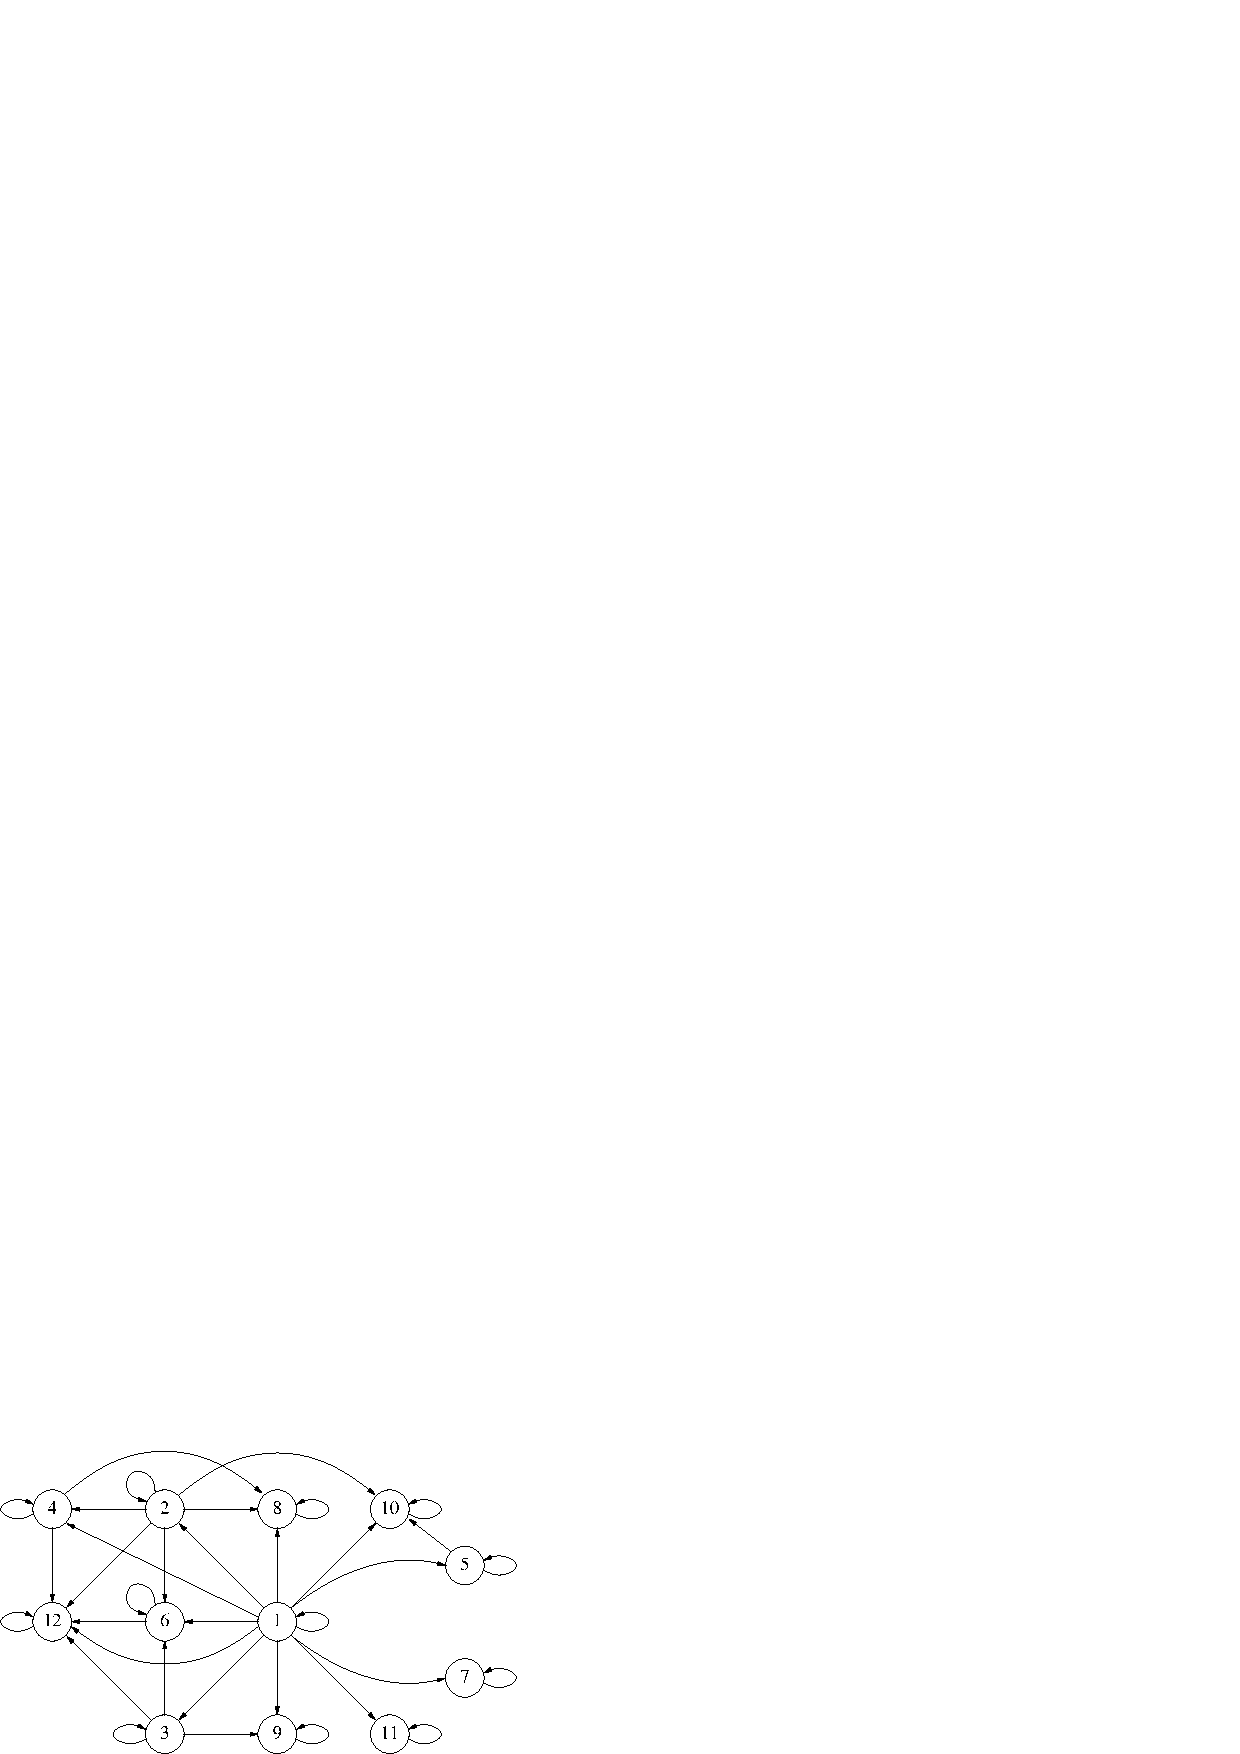
\includegraphics{figures/divisibility.pdf}
\caption{The Digraph for Divisibility on $\set{1,2,\dots,12}$.}
\label{fig:divisibility-digraph}
\end{figure}

%\hfill
%\includegraphics{divi2.pdf}
%{figures/divide12.mps}

\subsection{Paths in Digraphs}\label{paths}

Pictured with points and arrows, a length $k$ path in a digraph looks
like a line that starts at a point, $a_0$, and traverses $k$ arrows
between successive points, $a_1,a_2,\dots$ to end at a point, $a_k$.
A path is \term{simple} when it doesn't cross itself.  Here's the
precise definition:

\begin{definition}
A \emph{path in a digraph} is a sequence of vertices $a_0,\dots,a_k$
with $k \ge 0$ such that $\diredge{a_i}{a_{i+1}}$ is an edge of the
digraph for $i = 0,1,\dots, k-1$.  The path is said to \emph{start} at
$a_0$, to \emph{end} at $a_k$, and the \emph{length} of the path is
defined to be $k$.  The path is \emph{simple} iff all the $a_i$'s are
different, that is, $a_i = a_j$ only if $i=j$.
\end{definition}
Note a single vertex counts as length zero path that begins and ends
at itself.

Many of the relational properties have geometric descriptions in terms of
digraphs.  For example:
\begin{description}

\item[Reflexivity:] All vertices have self-loops (a \emph{self-loop} at a
vertex is an arrow going from the vertex back to itself).

\item[Irreflexivity:] No vertices have self-loops.

\item[Asymmetry:] No self-loops and at most one (directed) edge between
any two vertices.

\item[Symmetry:] A binary relation $R$ is
\hyperdef{graphs}{symmetric}{\term{symmetric}} iff $aRb$ implies $bRa$ for
all $a,b$ in the domain of $R$.  So if there is an edge from $a$ to $b$,
there is also one in the reverse direction.  So edges may as well be
represented without arrows, indicating that they can be followed in either
direction.

\item[Transitivity:] Short-circuits---for any path through the graph,
there is an arrow from the first vertex to the last vertex on the path.
\end{description}

We can define some new relations based on paths.  Let $R$ be the edge
relation of a digraph.  Define relations $R^*$ and $R^+$ on the vertices
by the conditions that for all vertices $a,b$:
\begin{eqnarray*}
a\, R^*\, b &\eqdef& \mbox{there is a path in $R$ from $a$ to $b$},\\
a\, R^+\, b &\eqdef& \mbox{there is a positive length path in $R$ from $a$ to $b$}.
\end{eqnarray*}

$R^*$ is called the \emph{path relation}\footnote{In many texts, $R^*$ is
called the \emph{transitive closure} of $R$.} of $R$.  It follows from the
definition of path that $R^*$ is transitive.  It is also reflexive
(because of the length-zero paths) and it contains the graph of $R$
(because of the length-one paths).  $R^+$ is called the
\emph{positive-length path relation}; it also contains $\graph{R}$ and is
transitive.

\subsection{Composition of Relations}\label{relation_compose_subsec}

There is a simple way to extend \idx{composition} of functions to
composition of relations, and this gives another way to talk about
paths in digraphs.

Let $R: B\to C$ and $S: A \to B$ be relations.  Then the
\idx{composition} of $R$ with $S$ is the binary relation $(R \compose
S): A\to C$ defined by the rule
\[
a \mrel{(R \compose S)} c \eqdef\ \exists b \in B.\, (b \mrel{R} c)
\QAND (a \mrel{S} b).
\]
This agrees with the Definition~\ref{func_compose_def} of composition
in the special case when $R$ and $S$ are functions.
\iffalse
\footnote{Some texts define $R \compose S$ the other way around, that
  is, with $S$ applied to the result of applying $R$ first.}
\fi

Now when $R$ is a digraph, it makes sense to compose $R$ with itself.
Then if we let $R^n$ denote the composition of $R$ with itself $n$
times, it's easy to check that $R^n$ is the length-$n$ path relation:
\[
a  \mrel{R^n} b \qiff \mbox{ there is a length $n$ path in $R$ from $a$ to $b$}.
\]
This even works for $n=0$, if we adopt the convention that $R^0$ is the
identity relation $\ident{A}$ on the set, $A$, of vertices.  That is, $a
\mrel{\ident{A}} b$ iff $a = b$.

\subsection{Directed Acyclic Graphs}\label{sec:dag}

\begin{definition}
A \term{cycle} in a digraph is defined by a path that begins and ends
at the same vertex.  Note that by convention, a single vertex is
considered to be a cycle of length 0 that begins and ends at the
vertex.  A \term{directed acyclic graph (DAG)} is a directed graph
with no positive length cycles.

A \term{simple cycle} in a digraph is a cycle whose vertices are distinct
except for the beginning and end vertices.
\end{definition}

\iffalse
In contrast to undirected graphs, a single vertex \emph{is} considered to
be a simple cycle.
\fi

DAG's are an economical way to represent partial orders.  For example, the
\emph{direct prerequisite} relation between MIT subjects in
Chapter~\ref{partial-order-chapter} was used to determine the partial
order of indirect prerequisites on subjects.  This indirect prerequisite
partial order is precisely the positive length path relation of the direct
prerequisites.

\begin{lemma}
If $D$ is a DAG, then $D^+$ is a strict partial order.
\end{lemma}

\begin{proof}
We know that $D^+$ is transitive.  Also, a positive length path from a
vertex to itself would be a cycle, so there are no such paths.  This means
$D^+$ is irreflexive, which implies it is a strict partial order (see
problem~\ref{CP_strict_PO_irreflexive}).
\end{proof}

It's easy to check that conversely, the graph of any strict partial
order is a DAG.

The divisibility partial order can also be more economically represented by
the path relation in a DAG.  \hyperdef{divisibility}{DAG}{A DAG whose
\emph{path} relation is divisibility} on $\set{1,2,\dots,12}$ is shown in
Figure~\ref{fig:divisibility-DAG}; the arrowheads are omitted in the
Figure, and edges are understood to point upwards.

\begin{figure}[h]
%\centering \includegraphics{figures/divi2.pdf}
\begin{center}
\setlength{\unitlength}{1973sp}%
%
\begingroup\makeatletter\ifx\SetFigFont\undefined%
\gdef\SetFigFont#1#2#3#4#5{%
  \reset@font\fontsize{#1}{#2pt}%
  \fontfamily{#3}\fontseries{#4}\fontshape{#5}%
  \selectfont}%
\fi\endgroup%
\begin{picture}(5452,6034)(10475,-13269)
{\color[rgb]{0,0,0}\thinlines
\put(13210,-12952){\circle{618}}
}%
\put(13210,-13027){\makebox(0,0)[b]{\smash{{\SetFigFont{12}{24.0}{\rmdefault}{\mddefault}{\updefault}{\color[rgb]{0,0,0}1}%
}}}}
{\color[rgb]{0,0,0}\put(13192,-9352){\circle{618}}
}%
\put(13192,-9427){\makebox(0,0)[b]{\smash{{\SetFigFont{12}{24.0}{\rmdefault}{\mddefault}{\updefault}{\color[rgb]{0,0,0}4}%
}}}}
{\color[rgb]{0,0,0}\put(13192,-7552){\circle{618}}
}%
\put(13192,-7627){\makebox(0,0)[b]{\smash{{\SetFigFont{12}{24.0}{\rmdefault}{\mddefault}{\updefault}{\color[rgb]{0,0,0}8}%
}}}}
{\color[rgb]{0,0,0}\put(14410,-11170){\circle{618}}
}%
\put(14410,-11245){\makebox(0,0)[b]{\smash{{\SetFigFont{12}{24.0}{\rmdefault}{\mddefault}{\updefault}{\color[rgb]{0,0,0}5}%
}}}}
{\color[rgb]{0,0,0}\put(13810,-10252){\circle{618}}
}%
\put(13810,-10327){\makebox(0,0)[b]{\smash{{\SetFigFont{12}{24.0}{\rmdefault}{\mddefault}{\updefault}{\color[rgb]{0,0,0}10}%
}}}}
{\color[rgb]{0,0,0}\put(12592,-10252){\circle{618}}
}%
\put(12592,-10327){\makebox(0,0)[b]{\smash{{\SetFigFont{12}{24.0}{\rmdefault}{\mddefault}{\updefault}{\color[rgb]{0,0,0}6}%
}}}}
{\color[rgb]{0,0,0}\put(11992,-11170){\circle{618}}
}%
\put(11992,-11245){\makebox(0,0)[b]{\smash{{\SetFigFont{12}{24.0}{\rmdefault}{\mddefault}{\updefault}{\color[rgb]{0,0,0}3}%
}}}}
{\color[rgb]{0,0,0}\put(12592,-8452){\circle{618}}
}%
\put(12592,-8527){\makebox(0,0)[b]{\smash{{\SetFigFont{12}{24.0}{\rmdefault}{\mddefault}{\updefault}{\color[rgb]{0,0,0}12}%
}}}}
{\color[rgb]{0,0,0}\put(15610,-11152){\circle{618}}
}%
\put(15610,-11227){\makebox(0,0)[b]{\smash{{\SetFigFont{12}{24.0}{\rmdefault}{\mddefault}{\updefault}{\color[rgb]{0,0,0}7}%
}}}}
{\color[rgb]{0,0,0}\put(10792,-11170){\circle{618}}
}%
\put(10792,-11245){\makebox(0,0)[b]{\smash{{\SetFigFont{12}{24.0}{\rmdefault}{\mddefault}{\updefault}{\color[rgb]{0,0,0}11}%
}}}}
{\color[rgb]{0,0,0}\put(11992,-9370){\circle{618}}
}%
\put(11992,-9445){\makebox(0,0)[b]{\smash{{\SetFigFont{12}{24.0}{\rmdefault}{\mddefault}{\updefault}{\color[rgb]{0,0,0}9}%
}}}}
{\color[rgb]{0,0,0}\put(13210,-11152){\circle{618}}
}%
\put(13210,-11227){\makebox(0,0)[b]{\smash{{\SetFigFont{12}{24.0}{\rmdefault}{\mddefault}{\updefault}{\color[rgb]{0,0,0}2}%
}}}}
{\color[rgb]{0,0,0}\put(13201,-12661){\line( 0, 1){1200}}
}%
{\color[rgb]{0,0,0}\put(13201,-10861){\line( 0, 1){1200}}
}%
{\color[rgb]{0,0,0}\put(13201,-9061){\line( 0, 1){1200}}
}%
{\color[rgb]{0,0,0}\put(13201,-9061){\line( 0, 1){1200}}
}%
{\color[rgb]{0,0,0}\put(12601,-9961){\line( 0, 1){1200}}
}%
{\color[rgb]{0,0,0}\put(12001,-10861){\line( 0, 1){1200}}
}%
{\color[rgb]{0,0,0}\put(12901,-11161){\makebox(3.3333,23.3333){\SetFigFont{5}{6}{\rmdefault}{\mddefault}{\updefault}.}}
}%
{\color[rgb]{0,0,0}\multiput(14251,-10910)(-10.28143,13.70857){29}{\makebox(3.3333,23.3333){\SetFigFont{5}{6}{\rmdefault}{\mddefault}{\updefault}.}}
}%
{\color[rgb]{0,0,0}\multiput(13009,-10914)(-10.28143,13.70857){29}{\makebox(3.3333,23.3333){\SetFigFont{5}{6}{\rmdefault}{\mddefault}{\updefault}.}}
}%
{\color[rgb]{0,0,0}\multiput(13028,-9107)(-10.28143,13.70857){29}{\makebox(3.3333,23.3333){\SetFigFont{5}{6}{\rmdefault}{\mddefault}{\updefault}.}}
}%
{\color[rgb]{0,0,0}\multiput(12168,-10904)(10.28143,13.70857){29}{\makebox(3.3333,23.3333){\SetFigFont{5}{6}{\rmdefault}{\mddefault}{\updefault}.}}
}%
{\color[rgb]{0,0,0}\multiput(13387,-10884)(10.28143,13.70857){29}{\makebox(3.3333,23.3333){\SetFigFont{5}{6}{\rmdefault}{\mddefault}{\updefault}.}}
}%
{\color[rgb]{0,0,0}\put(13017,-12714){\line(-2, 3){861.692}}
}%
{\color[rgb]{0,0,0}\put(12915,-12863){\line(-4, 3){1943.360}}
}%
{\color[rgb]{0,0,0}\put(13425,-12739){\line( 2, 3){861.692}}
}%
{\color[rgb]{0,0,0}\put(13517,-12849){\line( 4, 3){1943.360}}
}%
\end{picture}%

\end{center}
\caption{A DAG whose Path Relation is Divisibility on $\set{1,2,\dots,12}$.}
\label{fig:divisibility-DAG}
\end{figure}

If we're using a DAG just as an economical way to picture or represent its
path relation, we might want to replace it with the minimum edge DAG with
the same path relation.  This minimum edge DAG order is unique and easy to
find (see problem~\ref{CP_covering_edges}).

\begin{problems}
\practiceproblems
\pinput{TP_strictPOs_are_DAGs}

\classproblems
\pinput{CP_covering_edges}

\homeworkproblems
\pinput{PS_path_relation_composition}
\pinput{PS_finite_transitive_closure}
\end{problems}

%add problem building on matrix rep to compute transitive closure

\endinput



\chapter{State Machines}\label{state_machine_chap}

\providecommand{\boys}{\text{the-Boys}}
\providecommand{\girls}{\text{the-Girls}}
\providecommand{\qst}{\text{$q_0$}}
\providecommand{\none}{\texttt{none}}
\providecommand{\girln}{\text{$\girls \union \set{\none}$}}
\providecommand{\boyn}{\text{$\boys \union \set{\none}$}}
\providecommand{\sere}{\text{\emph{serenading}}}
\providecommand{\suit}{\text{\emph{suitors}}}
\providecommand{\fav}{\text{\emph{favorite}}}
\providecommand{\nex}{\text{\emph{next}}}
\providecommand{\tgn}{\text{\emph{total-girls-names}}}


\hyperdef{state}{machines}{\section{State machines}}\label{state_machine_sec}

State machines are an abstract model of step-by-step processes, and
accordingly, they come up in many areas of computer science.  You may
already have seen them in a digital logic course, a compiler course, or a
probability course.

\subsection{Basic definitions}

A state machine is really nothing more than a binary relation on a
set, except that the elements of the set are called ``states,'' the
relation is called the \term{transition relation}, and a pair $(p,q)$
in the graph of the transition relation is called a \term{transition}.
The transition from state $p$ to state $q$ will be written $p \movesto
q$.  The transition relation is also called the \term{state graph} of
the machine.  A state machine also comes equipped with a designated
\emph{start state}.

State machines used in digital logic and compilers usually have only a
finite number of states, but machines that model continuing computations
typically have an infinite number of states.  In many applications, the
states, and/or the transitions have labels indicating input or output
values, costs, capacities, or probabilities, but for our purposes,
unlabelled states and transitions are all we need.\footnote{We do name
states, as in Figure~\ref{fig:counter}, so we can talk about them, but the
names aren't part of the state machine.}

\begin{figure}[htbp]
\graphic{counter}
\caption{\em State transitions for the 99-bounded counter.}
\label{fig:counter}
\end{figure}

\begin{example}
A bounded counter, which counts from $0$ to $99$ and overflows at 100.
The transitions are pictured in Figure~\ref{fig:counter}, with start
state zero.  This machine isn't much use once it overflows, since it
has no way to get out of its overflow state.

\end{example}

\begin{example}
An unbounded counter is similar, but has an infinite state set.  This is
harder to draw \texttt{:-)}
\end{example}

\begin{example}
\textbf In the movie \textit{Die Hard 3: With a Vengeance}, the characters
played by Samuel L. Jackson and Bruce Willis have to disarm a bomb planted
by the diabolical Simon Gruber:

\textbox{
\begin{list}{}{\itemsep=0in \leftmargin=0.25in \rightmargin=0.25in}

\item[\textbf{Simon:}] On the fountain, there should be 2 jugs, do you
see them?  A 5-gallon and a 3-gallon.  Fill one of the jugs with
exactly 4 gallons of water and place it on the scale and the timer
will stop.  You must be precise; one ounce more or less will result in
detonation.  If you're still alive in 5 minutes, we'll speak.

\item[\textbf{Bruce:}] Wait, wait a second. I don't get it. Do you get it?

\item[\textbf{Samuel:}] No.

\item[\textbf{Bruce:}] Get the jugs. Obviously, we can't fill the 3-gallon jug
with 4 gallons of water.

\item[\textbf{Samuel:}] Obviously.

\item[\textbf{Bruce:}] All right. I know, here we go. We fill the 3-gallon jug
exactly to the top, right?

\item[\textbf{Samuel:}] Uh-huh.

\item[\textbf{Bruce:}] Okay, now we pour this 3 gallons into the 5-gallon jug,
giving us exactly 3 gallons in the 5-gallon jug, right?

\item[\textbf{Samuel:}] Right, then what?

\item[\textbf{Bruce:}] All right. We take the 3-gallon jug and fill it a third
of the way...

\item[\textbf{Samuel:}] No!  He said, ``Be precise.''  Exactly 4
gallons.

\item[\textbf{Bruce:}] Sh - -.  Every cop within 50 miles is running his a - - off
and I'm out here playing kids games in the park.

\item[\textbf{Samuel:}] Hey, you want to focus on the problem at hand?

\end{list}
}

Fortunately, they find a solution in the nick of time.  We'll let the
reader work out how.

The \emph{Die Hard} series is getting tired, so we propose a final
\emph{Die Hard Once and For All}.  Here Simon's brother returns to avenge
him, and he poses the same challenge, but with the 5 gallon jug replaced
by a 9 gallon one.

We can model jug-filling scenarios with a state machine.  In the scenario
with a 3 and a 5 gallon water jug, the states will be pairs, $(b,l)$ of
real numbers such that $0 \leq b \leq 5, 0 \leq l \leq 3$.  We let $b$ and
$l$ be arbitrary real numbers.  (We can prove that the values of $b$ and
$l$ will only be nonnegative integers, but we won't assume this.)  The
start state is $(0,0)$, since both jugs start empty.

Since the amount of water in the jug must be known exactly, we will only
consider moves in which a jug gets completely filled or completely
emptied.  There are several kinds of transitions:
\begin{enumerate}

\item  Fill the little jug: $(b,l) \movesto (b,3)$ for $l < 3$.

\item  Fill the big jug: $(b,l) \movesto (5,l)$ for $b<5$.

\item  Empty the little jug: $(b,l) \movesto (b,0)$ for $l>0$.

\item  Empty the big jug: $(b,l) \movesto (0,l)$ for $b>0$.

\item  Pour from the little jug into the big jug: for $l>0$,
\begin{equation*}
(b,l) \movesto
\begin{cases}
(b+l, 0) & \text{if $b + l \le 5$,}\\
(5, l - (5 - b)) & \text{otherwise.}
\end{cases}
\end{equation*}

\item Pour from big jug into little jug: for $b>0$,
\begin{equation*}
(b,l) \movesto
\begin{cases}
(0, b+l) & \text{if $b + l \le 3$,}\\
(b - (3 -l), 3) & \text{otherwise.}
\end{cases}
\end{equation*}
\end{enumerate}


Note that in contrast to the 99-counter state machine, there is more than
one possible transition out of states in the Die Hard machine.  Machines
like the 99-counter with at most one transition out of each state are
called \emph{deterministic}.  The Die Hard machine is
\emph{nondeterministic} because some states have transitions to several
different states.

\textbf{Quick exercise:} Which states of the Die Hard 3 machine have
direct transitions to exactly two states?

\end{example}

\subsection{Reachability and Preserved Invariants}

The Die Hard 3 machine models every possible way of pouring water among
the jugs according to the rules.  Die Hard properties that we want to
verify can now be expressed and proved using the state machine model.  For
example, Bruce's character will disarm the bomb if he can get to some
state of the form $(4, l)$.

A (possibly infinite) path through the state graph beginning at the
start state corresponds to a possible system behavior; such a path is
called an \term{execution} of the state machine.  A state is called
\term{reachable} if it appears in some execution.  The bomb in Die
Hard 3 gets disarmed successfully because the state (4,3) is
reachable.

\hyperdef{invariant}{properties}{A} useful approach in analyzing state
machine is to identify properties of states that are preserved by
transitions.  

\begin{definition}
  A \term{preserved invariant} of a state machine is a predicate, $P$, on
  states, such that whenever $P(q)$ is true of a state, $q$, and $q
  \movesto r$ for some state, $r$, then $P(r)$ holds.
\end{definition}

\textbox{\begin{center}
{\Large The Invariant Principle}
\end{center}

{\large
\noindent If a preserved invariant of a state machine is true for the
start state,\\
then it is true for all reachable states.}}

The Invariant Principle is nothing more than the Induction Principle
reformulated in a convenient form for state machines.  Showing that a
predicate is true in the start state is the base case of the induction,
and showing that a predicate is a preserved invariant is the inductive
step.\footnote{Preserved invariants are commonly just called
  ``invariants'' in the literature on program correctness, but we decided
  to throw in the extra adjective to avoid confusion with other
  definitions.  For example, another subject at MIT uses ``invariant'' to
  mean ``predicate true of all reachable states.''  Let's call this
  definition ``invariant-2.''  Now invariant-2 seems like a reasonable
  definition, since unreachable states by definition don't matter, and all
  we want to show is that a desired property is invariant-2.  But this
  confuses the \emph{objective} of demonstrating that a property is
  invariant-2 with the \emph{method} for showing that it is.  After all,
  if we already knew that a property was invariant-2, we'd have no need
  for an Invariant Principle to demonstrate it.}

\subsubsection{Die Hard Once and For All}

Now back to Die Hard Once and For All.  This time there is a 9 gallon jug
instead of the 5 gallon jug.  We can model this with a state machine whose
states and transitions are specified the same way as for the Die Hard 3
machine, with all occurrences of ``5'' replaced by ``9.''

Now reaching any state of the form $(4,l)$ is impossible.  We prove this
using the Invariant Principle.  Namely, we define the preserved invariant
predicate, $P(b,l)$, to be that $b$ and $l$ are nonnegative integer
multiples of 3.  So $P$ obviously holds for the state state $(0,0)$.

To prove that $P$ is a preserved invariant, we assume $P(b,l)$ holds for
some state $(b,l)$ and show that if $(b,l) \movesto (b',l')$, then
$P(b',l')$.  The proof divides into cases, according to which transition
rule is used.  For example, suppose the transition followed from the
``fill the little jug'' rule.  This means $(b,l) \movesto (b,3)$.  But
$P(b,l)$ implies that $b$ is an integer multiple of 3, and of course 3 is
an integer multiple of 3, so $P$ still holds for the new state $(b,3)$.
Another example is when the transition rule used is ``pour from big jug
into little jug'' for the subcase that $b + l > 3$.  Then state is $(b,l)
\movesto (b -( 3 -l), 3)$.  But since $b$ and $l$ are integer multiples of
3, so is $b -( 3 -l)$.  So in this case too, $P$ holds after the
transition.

We won't bother to crank out the remaining cases, which can all be checked
just as easily.  Now by the Invariant Principle, we conclude that every
reachable state satisifies $P$.  But since no state of the form $(4,l)$
satisifies $P$, we have proved rigorously that Bruce dies once and for
all!

By the way, notice that the state (1,0), which satisfies $\QNOT(P)$, has a
transition to (0,0), which satisfies $P$.  So it's wrong to assume that
the complement of a preserved invariant is also a preserved invariant.

\subsubsection{A Robot on a Grid}

There is a robot.  It walks around on a grid, and at every step it moves
diagonally in a way that changes its position by one unit up or down
\emph{and} one unit left or right.  The robot starts at position $(0, 0)$.
Can the robot reach position $(1, 0)$?

To get some intuition, we can simulate some robot moves.  For example,
starting at (0,0) the robot could move northeast to (1,1), then southeast
to (2,0), then southwest to (1,-1), then southwest again to (0,-2).

Let's model the problem as a state machine and then find a suitable
invariant.  A state will be a pair of integers corresponding to the
coordinates of the robot's position.  State $(i,j)$ has transitions to
four different states: $(i \pm 1, j \pm 1)$.

The problem is now to choose an appropriate preserved invariant, $P$, that
is true for the start state $(0,0)$ and false for $(1, 0)$.  The Invariant
Theorem then will imply that the robot can never reach $(1, 0)$.  A direct
attempt for a preserved invariant is the predicate $P(q)$ that $q \neq (1,
0)$.

Unfortunately, this is not going to work.  Consider the state $(2,1)$.
Clearly $P(2,1)$ holds because $(2,1) \neq (1, 0)$.  And of course
$P(1,0)$ does not hold.  But $(2,1) \movesto (1,0)$, so this choice of $P$
will not yield a preserved invariant.

We need a stronger predicate.  Looking at our example execution you might
be able to guess a proper one, namely, that the sum of the coordinates is
even!  If we can prove that this is a preserved invariant, then we have
proven that the robot never reaches $(1, 0)$ ---because the sum $1+0$ of
its coordinates is odd, while the sum $0+0$ of the coordinates of the
start state is even.

\begin{theorem}
The sum of the robot's coordinates is always even.
\end{theorem}

\begin{proof}
The proof uses the Invariant Principle.

Let $P(i, j)$ be the predicate that $i + j$ is even.

First, we must show that the predicate holds for the start state $(0,0)$.
Clearly, $P(0, 0)$ is true because $0 + 0$ is even.

Next, we must show that $P$ is a preserved invariant.  That is, we must
show that for each transition $(i, j) \movesto (i', j')$, if $i + j$ is
even, then $i' + j'$ is even.  But $i' = i \pm 1$ and $j' = j \pm 1$ by
definition of the transitions.  Therefore, $i' + j'$ is equal to $i + j$
or $i + j \pm 2$, all of which are even.
\end{proof}

\begin{corollary}
The robot cannot reach $(1, 0)$.
\end{corollary}

\textbox{
\begin{center}
{\Large Robert W. Floyd}
\end{center}

The Invariant Principle was formulated by Robert Floyd at Carnegie
Tech\footnote{The following year, Carnegie Tech was renamed
  Carnegie-Mellon Univ.} in 1967.  Floyd was already famous for work on
formal grammars which transformed the field of programming language
parsing; that was how he got to be a professor even though he never got a
Ph.D.  (He was admitted to a PhD program as a teenage prodigy, but flunked
out and never went back.)

In that same year, Albert R. Meyer was appointed Assistant Professor in
the Carnegie Tech Computer Science Department where he first met Floyd.
Floyd and Meyer were the only theoreticians in the department, and they
were both delighted to talk about their shared interests.  After just a
few conversations, Floyd's new junior colleague decided that Floyd was the
smartest person he had ever met.

Naturally, one of the first things Floyd wanted to tell Meyer about was
his new, as yet unpublished, Invariant Principle.  Floyd explained the
result to Meyer, and Meyer wondered (privately) how someone as brilliant
as Floyd could be excited by such a trivial observation.  Floyd had to
show Meyer a bunch of examples before Meyer understood Floyd's excitement
---not at the truth of the utterly obvious Invariant Principle, but rather
at the insight that such a simple theorem could be so widely and easily
applied in verifying programs.

Floyd left for Stanford the following year.  He won the Turing award
---the ``Nobel prize'' of computer science--- in the late 1970's, in
recognition both of his work on grammars and on the foundations of
program verification.  He remained at Stanford from 1968 until his
death in September, 2001.  You can learn more about Floyd's life and
work by reading the
\href{http://courses.csail.mit.edu/6.042/spring10/floyd-eulogy-by-knuth.pdf}{eulogy}
written by his closest colleague, Don Knuth.

 \iffalse
   \href{http://oldwww.acm.org/pubs/membernet/stories/floyd.pdf}
{\texttt{http://oldwww.acm.org/pubs/membernet/stories/floyd.pdf}}.
\fi
}

\subsection{Sequential algorithm examples}\label{seq_alg_subsec}

\subsubsection{Proving Correctness}

Robert Floyd, who pioneered modern approaches to program verification,
distinguished two aspects of state machine or process correctness:

\begin{enumerate}
\item The property that the final results, if any, of the process satisfy
system requirements.  This is called \emph{partial correctness}.

You might suppose that if a result was only partially correct, then it
might also be partially incorrect, but that's not what he meant.  The word
``partial'' comes from viewing a process that might not terminate as
computing a \emph{partial function}.  So partial correctness means that
when there is a result, it is correct, but the process might not always
produce a result, perhaps because it gets stuck in a loop.

\item The property that the process always finishes, or is guaranteed to
produce some legitimate final output.  This is called \emph{termination}.
\end{enumerate}

Partial correctness can commonly be proved using the Invariant Principle.
Termination can commonly be proved using the Well Ordering Principle.
We'll illustrate Floyd's ideas by verifying the Euclidean Greatest Common
Divisor (GCD) Algorithm.

\subsubsection{The Euclidean Algorithm}\label{euclid}

The \index{GCD algorithm}\term{Euclidean algorithm} is a
three-thousand-year-old procedure to compute the greatest common divisor,
$\gcd(a,b)$ of integers $a$ and $b$.  We can represent this algorithm as a
state machine.  A state will be a pair of integers $(x,y)$ which we can
think of as integer registers in a register program.  The state
transitions are defined by the rule
\[
(x,y) \movesto (y, \remainder(x,y))
\]
for $y \neq 0$.  The algorithm terminates when no further transition is
possible, namely when $y=0$.  The final answer is in $x$.

We want to prove:
\begin{enumerate}
\item Starting from the state with $x = a$ and $y = b>0$, if we ever finish,
then we have the right answer.  That is, at termination, $x = \gcd(a,b)$.
This is a \emph{partial correctness} claim.

\item We do actually finish.  This is a process \emph{termination} claim.

\end{enumerate}

\paragraph{Partial Correctness of GCD}

First let's prove that if GCD gives an answer, it is a correct answer.
Specifically, let $d \eqdef \gcd(a,b)$.  We want to prove that \emph{if}
the procedure finishes in a state $(x,y)$, then $x = d$.

\begin{proof}
Define the state predicate
\[
P(x,y) \eqdef\ \ [\gcd(x,y) = d \text{ and } (x > 0 \text{ or } y > 0)].
\]

$P$ holds for the start state $(a,b)$, by definition of $d$ and the
requirement that $b$ is positive.  Also, the preserved invariance of
$P$ follows immediately from
\begin{lemma}\label{gcdlem}
For all $m,n \in \naturals$ such that $n \neq 0$,
\begin{equation}
\gcd(m,n) = \gcd(n,\remainder(m,n)).
\end{equation}
\end{lemma}

Lemma~\ref{gcdlem} is easy to prove: let $q$ be the quotient and $r$
be the remainder of $m$ divided by $n$.  Then $m = qn +r$ by
definition.  So any factor of both $r$ and $n$ will be a factor of
$m$, and similarly any factor of both $m$ and $n$ will be a factor of
$r$.  So $r,n$ and $m,n$ have the same common factors and therefore
the same gcd.  Now by the Invariant Principle, $P$ holds for all
reachable states.

Since the only rule for termination is that $y=0$, it follows that if
$(x,y)$ is a terminal state, then $y=0$.  If this terminal state is
reachable, then the preserved invariant holds for $(x,y)$.  This implies
that $\gcd(x,0) = d$ and that $x>0$.  We conclude that $x = \gcd(x,0) =
d$.
\end{proof}

\paragraph{Termination of GCD}

Now we turn to the second property, that the procedure must terminate.  To
prove this, notice that $y$ gets strictly smaller after any one
transition.  That's because the value of $y$ after the transition is the
remainder of $x$ divided by $y$, and this remainder is smaller than $y$ by
definition.  But the value of $y$ is always a nonnegative integer, so by the
Well Ordering Principle, it reaches a minimum value among all its values
at reachable states.  But there can't be a transition from a state where
$y$ has its minimum value, because the transition would decrease $y$ still
further.  So the reachable state where $y$ has its minimum value is a
state at which no further step is possible, that is, at which the
procedure terminates.

Note that this argument does not prove that the minimum value of $y$ is
zero, only that the minimum value occurs at termination.  But we already
noted that the only rule for termination is that $y=0$, so it follows that
the minimum value of $y$ must indeed be zero.

\subsubsection{The Extended Euclidean Algorithm}\label{ExtendedGCD}

An important fact about the $\gcd(a,b)$ is that it equals an integer
linear combination of $a$ and $b$, that is,
\begin{equation}\label{sa}
\gcd(a,b) = sa+ tb
\end{equation}
for some $s,t \in \integers$.  We'll see some nice proofs
of~\eqref{sa} later when we study Number Theory, but now we'll look
at an extension of the Euclidean Algorithm that efficiently, if
obscurely, produces the desired $s$ and $t$.  It is presented here
simply as another example of application of the Invariant Method
(plus, we'll need a procedure like this when we take up number theory
based cryptography in a couple of weeks).

\emph{Don't worry if you find this Extended Euclidean Algorithm hard to
  follow, and you can't imagine where it came from.  In fact, that's good,
  because this will illustrate an important point: given the right
  preserved invariant, you can verify programs you don't understand.}

In particular, given nonnegative integers $x$ and $y$, with $y>0$, we
claim the following procedure\footnote{This procedure is adapted from Aho,
  Hopcroft, and Ullman's text on algorithms.}  halts with registers
\texttt{S} and \texttt{T} containing integers $s$ and $t$
satisfying~\eqref{sa}.

Inputs: $a,b \in \naturals, b>0$.

Registers: \texttt{X,Y,S,T,U,V,Q}.

Extended Euclidean Algorithm:
\begin{center}
\begin{verbatim}
X := a; Y := b; S := 0; T := 1; U := 1; V := 0; 
loop:
if Y divides X, then halt
else
  Q := quotient(X,Y);
         ;;the following assignments in braces are SIMULTANEOUS
 {X := Y,
  Y := remainder(X,Y);
  U := S,
  V := T,
  S := U - Q * S,
  T := V - Q * T};
goto loop;
\end{verbatim}
\end{center}

Note that \texttt{X,Y} behave exactly as in the Euclidean GCD algorithm in
Section~\ref{euclid}, except that this extended procedure stops one step
sooner, ensuring that $\gcd(x,y)$ is in \texttt{Y} at the end.  So for all
inputs $x,y$, this procedure terminates for the same reason as the
Euclidean algorithm: the contents, $y$, of register \texttt{Y} is a
nonnegative integer-valued variable that strictly decreases each time
around the loop.

The following properties are preserved invariants that imply partial
correctness:
\begin{eqnarray}
\gcd(X,Y) &=& \gcd(a,b), \label{XY}\\
Sa+Tb &=& Y,\text{ and }\label{SaTb}\\
Ua+Vb &=& X. \label{uaVb}
\end{eqnarray}

To verify that these are preserved invariants, note that~\eqref{XY} is the
same one we observed for the Euclidean algorithm.  To check the other two
properties, let $x,y,s,t,u,v$ be the contents of registers
\texttt{X,Y,S,T,U,V} at the start of the loop and assume that all the
properties hold for these values.  We must prove that~\eqref{SaTb}
and~\eqref{uaVb} hold (we already know~\eqref{XY} does) for the new
contents $x',y',s',t',u',v'$ of these registers at the next time the loop
is started.

Now according to the procedure, $u'=s,v'=t,x'=y$, so~\eqref{uaVb} holds
for $u',v',x'$ because of~\eqref{SaTb} for $s,t,y$.  Also, 
\[
s'= u - qs,\quad t'= v - qt,\quad y' = x - qy
\]
where $q = \quotient(x,y)$,
so
\[
s'a+t'b = (u-qs)a + (v-qt)b =ua+vb - q(sa+tb) = x - qy = y',
\]
and therefore~\eqref{SaTb} holds for $s',t',y'$.

Also, it's easy to check that all three preserved invariants are true just
before the first time around the loop.  Namely, at the start:
\begin{align*}
X      =a, Y=b,S=0, T& =1 & \mbox{so}\\
Sa+Tb = 0a+1b=b& =Y & \mbox{confirming~\eqref{SaTb}.}
\end{align*}
Also,
\begin{align*}
U     & =1, V=0, & \mbox{so} \\
Ua+Vb & = 1a+0b=a =X & \mbox{confirming~\eqref{uaVb}.  }
\end{align*}
Now by the Invariant Principle, they are true at termination.  But at
termination, the contents, $Y$, of register \texttt{Y} divides the
contents, $X$, of register \texttt{X}, so preserved invariants~\eqref{XY}
and~\eqref{SaTb} imply
\[
\gcd(a,b) = \gcd(X,Y) = Y = Sa + Tb.
\]
So we have the gcd in register \texttt{Y} and the desired coefficients in
\texttt{S}, \texttt{T}.

Now we don't claim that this verification offers much insight.  In fact,
if you're not wondering how somebody came up with this concise program and
invariant, you:
\begin{itemize}

\item are blessed with an inspired intellect allowing you to see how this
  program and its invariant were devised,

\item have lost interest in the topic, or

\item haven't read this far.

\end{itemize}
If none of the above apply to you, we can offer some reassurance by
repeating that you're not expected to understand this program.

We've already observed that a preserved invariant is really just an
induction hypothesis.  As with induction, finding the right hypothesis
is usually the hard part.  We repeat:
\begin{quote}
  \textbf{Given the right preserved invariant, it can be easy to verify a
    program even if you don't understand it.}
\end{quote}
We expect that the Extended Euclidean Algorithm presented above
illustrates this point.

\subsection{Derived Variables}\label{derived_var_subsec}

The preceding termination proofs involved finding a nonnegative
integer-valued measure to assign to states.  We might call this measure
the ``size'' of the state.  We then showed that the size of a state
decreased with every state transition.  By the Well Ordering Principle,
the size can't decrease indefinitely, so when a minimum size state is
reached, there can't be any transitions possible: the process has
terminated.

\hyperdef{derived}{vars}{More} generally, the technique of assigning
values to states ---not necessarily nonnegative integers and not necessarily
decreasing under transitions--- is often useful in the analysis of
algorithms.  \emph{Potential functions} play a similar role in physics.
In the context of computational processes, such value assignments for
states are called \emph{derived variables}.

For example, for the Die Hard machines we could have introduced a derived
variable, $f: \text{states } \to \reals$, for the amount of water in both
buckets, by setting $f((a, b)) \eqdef a + b$.  Similarly, in the robot
problem, the position of the robot along the $x$-axis would be given by
the derived variable $x\text{-coord}$, where $x\text{-coord}((i, j))
\eqdef~i$.

We can formulate our general termination method as follows:

\begin{definition}
  Let $\prec$ be a strict partial order on a set, $A$.  A derived variable
  $f : \text{states } \to A$ is \emph{strictly decreasing} iff
\[
q \movesto q' \text{  implies  } f(q') \prec f(q).
\]
\end{definition}

We confirmed termination of the GCD and Extended GCD procedures by finding
derived variables, $y$ and \texttt{Y}, respectively, that were nonnegative
integer-valued and strictly decreasing.  We can summarize this approach to
proving termination as follows:
\begin{theorem}
\label{th:decr}
If $f$ is a strictly decreasing $\naturals$-valued derived variable of a
state machine, then the length of any execution starting at state $q$ is
at most $f(q)$.
\end{theorem}

Of course we could prove Theorem~\ref{th:decr} by induction on the value
of $f(q)$, but think about what it says: ``If you start counting down at
some nonnegative integer $f(q)$, then you can't count down more than
$f(q)$ times.''  Put this way, it's obvious.

\subsubsection{Weakly Decreasing Variables}

In addition being strictly decreasing, it will be useful to have derived
variables with some other, related properties.

\begin{definition}
Let $\preceq$ be a weak partial order on a set, $A$.  A derived variable
$f : Q \to A$ is \emph{weakly decreasing} iff
\[
q \movesto q' \text{  implies  } f(q') \preceq f(q).
\]

\emph{Strictly increasing} and \emph{weakly increasing} derived variables
are defined similarly.\footnote{Weakly increasing variables are often also
called \emph{nondecreasing}.  We will avoid this terminology to prevent
confusion between nondecreasing variables and variables with the much
weaker property of \emph{not} being a decreasing variable.}
\end{definition}

\begin{editingnotes}
\section*{Well-founded termination}
omitted

\iffalse

There are cases where it's easier to prove termination based on more
general partial orders than ``less-than'' on $\naturals$.  Termination is
guaranteed whenever there is a derived variable that strictly decreases with
respect to any well-founded partial order.

\iffalse
We now define some other useful flavors of derived variables taking values
over partial ordered sets.  We'll use the notational convention that when
$\prec$ denotes a strict partial order on some set, then $\preceq$ is the
corresponding \emph{weak} partial order
\[
a\preceq a' \ \eqdef\quad a \prec a' \lor a = a'.
\]
\fi

\begin{definition}
Let $\prec$ be a strict partial order on a set, $A$.  A derived variable
$f : Q \to A$ is \emph{strictly decreasing} with respect to $\prec$ iff
\[
q \movesto q' \text{ implies } f(q') \prec f(q).
\]
Also, $f$ is \emph{weakly decreasing} iff
\[
q \movesto q' \text{  implies  } f(q') \preceq f(q).
\]
where $\preceq$ is the weak partial order corresponding to $\prec$,
namely,
\[
[a_1 \preceq a_2] \eqdef [(a_1 \prec a_2) \text{ or } (a_1=a_2)].
\]

\emph{Strictly increasing} and \emph{weakly increasing} derived variables
are defined similarly.\footnote{Weakly increasing variables are often also
called \emph{nondecreasing}.  We will avoid this terminology to prevent
confusion between nondecreasing variables and variables with the much
weaker property of \emph{not} being a decreasing variable.}
\end{definition}

\begin{theorem}\label{well-founded-decreasing}
  If there exists a derived variable for a state machine that is strictly
  decreasing with respect to some well-founded partial order, then every
  execution terminates.
\end{theorem}

Theorem~\ref{well-founded-decreasing} follows immediately from the
\href{http://courses.csail.mit.edu/6.042/spring08/ln3.pdf#infinite.decreasing}
{observation in Notes 3} that a well-founded partial order has no infinite
decreasing sequences.

Note that the existence of a nonnegative integer-valued \emph{weakly}
decreasing derived variable does not guarantee that every execution
terminates.  That's because an infinite execution could proceed through
states in which a weakly decreasing variable remained constant.

\subsubsection{A Southeast Jumping Robot}

\iffalse Begin by defining the trivial ``pick how long'' game: P1 picks $n
\in \naturals$, the P2 and P1 alternate making forced moves.  The game
ends after $n$ forced moves; the last person to move wins.  So P1 strategy
is ``pick and even number.''  Insert here the discussion of ``terminates,
but no bound on number of steps...'' used below.

May also tell the ``guess a bigger number game''joke.
\fi

Here's a contrived but simple example of proving termination based on a
variable that is strictly decreasing over a well-founded order.  Let's
think about a robot positioned at an integer lattice-point in the
Northeast quadrant of the plane, that is, at $(x,y) \in \naturals^2$.

At every second when it is away from the origin, $(0,0)$, the robot must
make a move, which may be
\begin{itemize}

\item a unit distance West when it is not at the boundary of the Northeast
  quadrant (that is, $(x,y) \movesto (x-1,y)$ for $x>0$), or

\item a unit distance South combined with an arbitrary jump East (that is,
     $(x,y) \movesto (z,y-1)$ for $z\geq x$).

\end{itemize}
\begin{claim}\label{robotcl}
The robot will always get stuck at the origin.
\end{claim}

If we think of the robot as a nondeterministic state machine, then
Claim~\ref{robotcl} is a termination assertion.  The Claim may seem
obvious, but it really has a different character than termination based on
nonnegative integer-valued variables.  That's because, even knowing that
the robot is at position $(0,1)$, for example, there is no way to bound
the time it takes for the robot to get stuck.  It can delay getting stuck
for as many seconds as it wants by making its next move to a distant point
in the Far East.  This rules out proving termination using
Theorem~\ref{th:decr}.

So does Claim~\ref{robotcl} still seem obvious?

Well it is if you see the trick: if we reverse the coordinates, then every
robot move goes to a position that is smaller under lexicographic order.
More precisely, let $f:\naturals^2 \to \naturals^2$ be the derived variable
mapping a robot state ---its position $(x,y)$ ---to $(y,x) \in
\naturals^2$.  Now $(x,y)\movesto (x',y')$ is a legitimate robot move iff
$f((x',y')) \lex< f((x,y))$.  In particular, $f$ is a strictly
$\lex<$-decreasing derived variable, so
Theorem~\ref{well-founded-decreasing} proves that the robot always get
stuck as claimed.
\fi


\iffalse

We will prove that the robot always gets stuck at the origin by
generalizing the decreasing variable method, but with decreasing values
that are more general than nonnegative integers.  Namely, the traveling robot
can be modeled with a state machine with states of the form $((x,y),s,e)$
where
\begin{itemize}
\item $(x,y) \in \naturals^2$ is the robot's position,
\item $s$ is the number of moves South the robot took to get to this
position, and
\item $e \le 2s$ is the number of moves East the robot took to get to this
position. 
\end{itemize}

Now we define a derived variable $\vl:\text{States}\to \naturals^3$:
\[
\vl(((x,y),s,e)) \ \eqdef\quad (y,2s-e,x),
\]
and we order the values of states with the \emph{lexicographic} order,
$\lexle$, on $\naturals^3$:
\begin{equation}\label{lex3}
(k,l,m) \lexle (k',l',m') \ \eqdef\quad k < k' \text{ or } (k=k' \text{
and } l < l') \text{ or } (k=k' \text{ and } l = l' \text{ and } m \le m')
\end{equation}

Let's check that values are lexicographically decreasing.  Suppose the
robot is in state $((x,y),s,e)$.
\begin{itemize}
\item If the robot moves West it enters state $((x-1,y),s,e)$, and
\[
\vl(((x-1,y),s,e)) = (y,2s-e,x-1) \lex< (y,2s-e,x) = \vl(((x,y),s,e)),
\]
as required.


\item If the robot jumps East it enters a state $((z,y),s,e+1)$ for some
$z>x$.  Now
\[
\vl(((z,y),s,e+1)) = (y,2s-(e+1),z) = (y,2s-e-1,z),
\]
but since $2s-e-1 < 2s-e$, the rule~(\ref{lex3}) implies that
\[
\vl(((z,y),s,e+1)) = (y,2s-e-1,z)  \lex< (y,2s-e,x) = \vl(((x,y),s,e)),
\]
as required.

\item If the robot moves South it enters state $((x,y-1),s+1,e)$, and
\[
\vl(((x,y-1),s+1,e)) = (y-1,2(s+1)-e,x) \lex< (y,2s-e,x) = \vl(((x,y),s,e)),
\]
as required.

\end{itemize}

So indeed state-value is a decreasing variable under lexicographic order.
But since lexicographic order is well-founded, it is impossible for a
lexicographically-ordered value to be decreased an infinite number of
times.  That's just what we need to finish verifying Claim~\ref{robotcl}.
\fi

\end{editingnotes}


\begin{problems}
\homeworkproblems

\pinput{PS_filling_buckets_with_water}

\pinput{PS_linear_combination_game}

\pinput{PS_divide_using_3}

\pinput{PS_robot_on_2D_grid}

\pinput{PS_ant_on_grid}

\pinput{PS_card_shuffle_state_machine}

\pinput{PS_top_sort_for_closure_of_DAG}

\classproblems

\pinput{CP_fifteen_puzzle}

\pinput{CP_fast_exponentiation}

\pinput{CP_robot_invariant}

\pinput{CP_Zakim_bridge_state_machine}

\pinput{CP_98_heads_and_4_tails}

\pinput{CP_beaver_flu}

\end{problems}


\hyperdef{stable}{marriage}{\section{The Stable Marriage Problem}}
\label{stablemarriagesec}

\iffalse
\begin{center}
{\large \textbf{To Appear.}}
\end{center}
\fi


Okay, frequent public reference to derived variables may not help your
mating prospects.  But they can help with the analysis!

\subsection{The Problem}

Suppose there are a bunch of boys and an equal number of girls that we
want to marry off.  Each boy has his personal preferences about the girls
---in fact, we assume he has a complete list of all the girls ranked
according to his preferences, with no ties.  Likewise, each girl has a
ranked list of all of the boys.

The preferences don't have to be symmetric.  That is, Jennifer might like
Brad best, but Brad doesn't necessarily like Jennifer best.  The goal is
to marry off boys and girls: every boy must marry exactly one girl and
vice-versa---no polygamy.  In mathematical terms, we want the mapping
from boys to their wives to be a bijection or \emph{perfect matching}.
We'll just call this a ``matching,'' for short.

Here's the difficulty: suppose \emph{every} boy likes Angelina best, and
every girl likes Brad best, but Brad and Angelina are married to other
people, say Jennifer and Billy Bob.  Now \emph{Brad and Angelina prefer
each other to their spouses}, which puts their marriages at risk: pretty
soon, they're likely to start spending late nights doing 6.042 homework
together.

This situation is illustrated in the following diagram where the digits
``1'' and ``2'' near a boy shows which of the two girls he ranks first and
which second, and similarly for the girls:
\begin{figure}
\graphic{minWtMatch2}
\end{figure}
More generally, in any matching, a boy and girl who are not married to
each other and who like each other better than their spouses, is called a
{\em rogue couple}.  In the situation above, Brad and Angelina would be a
rogue couple.

Having a rogue couple is not a good thing, since it threatens the
stability of the marriages.  On the other hand, if there are no rogue
couples, then for any boy and girl who are not married to each other, at
least one likes their spouse better than the other, and so won't be
tempted to start an affair.

\begin{definition}
  A \term{stable matching} is a matching with no rogue couples.
\end{definition}
 
The question is, given everybody's preferences, how do you find a stable
set of marriages?  In the example consisting solely of the four people
above, we could let Brad and Angelina both have their first choices by
marrying each other.  Now neither Brad nor Angelina prefers anybody else
to their spouse, so neither will be in a rogue couple.  This leaves Jen
not-so-happily married to Billy Bob, but neither Jen nor Billy Bob can
entice somebody else to marry them.
 
It is something of a surprise that there always is a stable matching among
a group of boys and girls, but there is, and we'll shortly explain why.
The surprise springs in part from considering the apparently similar
``buddy'' matching problem.  That is, if people can be paired off as
buddies, regardless of gender, then a stable matching \emph{may not} be
possible.  For example, Figure~\ref{fig:buddy} shows a situation with a
love triangle and a fourth person who is everyone's last choice.  In this
figure Mergatoid's preferences aren't shown because they don't even
matter.   

\begin{figure}[htbp]
\graphic{loveTriangle}
\caption{Some preferences with no stable buddy matching.}
\label{fig:buddy}
\end{figure}
 
Let's see why there is no stable matching: 
\begin{lemma*}
There is no stable buddy matching among the four people in
Figure~\ref{fig:buddy}.
\end{lemma*}
 
\begin{proof}
We'll prove this by contradiction.

Assume, for the purposes of contradiction, that there is a stable
matching.  Then there are two members of the love triangle that are
matched.  Since preferences in the triangle are symmetric, we may assume
in particular, that Robin and Alex are matched.  Then the other pair must
be Bobby-Joe matched with Mergatoid.

But then there is a rogue couple: Alex likes Bobby-Joe best, and Bobby-Joe
prefers Alex to his buddy Mergatoid.  That is, Alex and Bobby-Joe are a
rogue couple, contradicting the assumed stability of the matching.
\end{proof}

So getting a stable \emph{buddy} matching may not only be hard, it may be
impossible.  But when boys are only allowed to marry girls, and vice
versa, then it turns out that a stable matching is not hard to find.

%%insert rest of story from gusfield book pp3--4??

\iffalse

\subsection{Failed attempts}

Let's find a stable matching in one possible situation, and hope to
translate our method to a general algorithm.  The table below shows the
preferences of each girl and boy in decreasing order.

\begin{eqnarray*}
boys & \quad & girls \\
1 : C B E A D & \quad & A : 3 5 2 1 4 \\
2 : A B E C D & \quad & B : 5 2 1 4 3 \\
3 : D C B A E & \quad & C : 4 3 5 1 2 \\
4 : A C D B E & \quad & D : 1 2 3 4 5 \\
5 : A B D E C & \quad & E : 2 3 4 1 5
\end{eqnarray*}

How about we try a ``greedy'' strategy?\footnote{``Greedy'' is not any
moral judgment.  It refers to algorithms that work by always choosing the
next state that makes the largest immediate progress.}  We simply take
each boy in turn and pack him off with his favorite among the girls still
available.  This gives the following assignment.

\begin{eqnarray*}
1 \rightarrow C \\
2 \rightarrow A \\
3 \rightarrow D \\
4 \rightarrow B \\
5 \rightarrow E \\
\end{eqnarray*}

To determine whether this matching is stable, we have to check whether
there are any rogue couples.  Boys 1, 2, and 3 all got their top pick
among the girls; none would even think of running off.  Boy 4 may be a
problem because he likes girl $A$ better than his mate, but she ranks him
dead last.  However, boy 4 also likes girl $C$ better than his mate, and
she rates him above her own mate.  Therefore, boy 4 and girl $C$ form a
rogue couple!  The marriages are not stable.  We could try to make ad hoc
repairs, but we're really trying to develop a general strategy.

Another approach would be to use induction.  Suppose we pair Boy 1 with
his favorite girl, $C$, try to show that neither of these two will be
involved in a rogue couple, and then solve the remaining problem by
induction.  Clearly Boy 1 will never leave his top pick, Girl $C$.  But
the problem with this approach is that we \emph{can't} be sure that Girl
$C$ won't be in a rogue couple.  Girl $C$ might very well dump Boy 1 --
she might even rate him last!

This turns out to be a tricky problem.  The best approach is to use a
mating ritual that is reputed to have been popular in some mythic past.
\fi

\subsection{The Mating Ritual}

The procedure for finding a stable matching involves a \emph{Mating
Ritual} that takes place over several days.  The following events happen
each day:

{\bf Morning: } Each girl stands on her balcony.  Each boy stands under
the balcony of his favorite among the girls on his list, and he serenades
her.  If a boy has no girls left on his list, he stays home and does his
6.042 homework.

{\bf Afternoon: } Each girl who has one or more suitors serenading
her, says to her favorite among them, ``We might get engaged.  Come
back tomorrow.''  To the other suitors, she says, ``No.  I will never
marry you!  Take a hike!''

\textbf{Evening}: Any boy who is told by a girl to take a hike, crosses that
girl off his list.

\textbf{Termination condition}: When every girl has at most one suitor,
the ritual ends with each girl marrying her suitor, if she has one.

% Show example

There are a number of facts about this Mating Ritual that we would like to
prove:

\begin{itemize}
\item The Ritual has a last day.
\item Everybody ends up married.
\item The resulting marriages are stable.
\end{itemize}

\subsection{A State Machine Model}

Before we can prove anything, we should have clear mathematical
definitions of what we're talking about.  In this section we sketch how to
define a rigorous state machine model of the Marriage Problem.

So let's begin by formally defining the problem.

\begin{definition}
  A \term{Marriage Problem} consists of two disjoint sets of the same
  finite size, called \boys\ and \girls.  The members of \boys\ are called
  \emph{boys}, and members of \girls\ are called \emph{girls}.  For each
  boy, $B$, there is a strict total order, \term{$<_B$}, on \girls, and
  for each girl, $G$, there is a strict total order, \term{$<_G$}, on
  \boys.  If $G_1 <_B G_2$ we say $B$ \term*{prefers} girl $G_2$ to girl
  $G_1$.  Similarly, if $B_1 <_G B_2$ we say $G$ \term{prefers} boy $B_2$
  to boy $B_1$.

A \term{marriage assignment} or \term{perfect matching} is a bijection,
$w:\boys \to \girls$.  If $B \in \boys$, then $w(B)$ is called $B$'s
\emph{wife} in the assignment, and if $G \in \girls$, then $w^{-1}(G)$ is
called $G$'s \emph{husband}.  A \term{rogue couple} is a boy, $B$, and a
girl, $G$, such that $B$ prefers $G$ to his wife, and $G$ prefers $B$ to
her husband.  An assignment is \term{stable} if it has no rogue couples.
A \term{solution} to a marriage problem is a stable perfect matching.
\end{definition}

To model the Mating Ritual with a state machine, we make a key
observation: to determine what happens on any day of the Ritual, all we
need to know is which girls are still on which boys' lists on the morning of
that day.  So we define a state to be some mathematical data structure
providing this information.  For example, we could define a state to be
the ``still-has-on-his-list'' relation, $R$, between boys and girls, where
$B\mrel{R}G$ means girl $G$ is still on boy $B$'s list.

We start the Mating Ritual with no girls crossed off.  That is, the start
state is the \emph{\idx{complete bipartite}} relation in which every boy
is related to every girl.

According to the Mating Ritual, on any given morning, a boy will
\term{serenade} the girl he most prefers among those he has not as yet
crossed out.  Mathematically, the girl he is serenading is just the
maximum among the girls on $B$'s list, ordered by $<_B$.  (If the list is
empty, he's not serenading anybody.)  A girl's \term{favorite} is just the
maximum, under her preference ordering, among the boys serenading her.

Continuing in this way, we could mathematically specify a precise Mating
Ritual state machine, but we won't bother.  The intended behavior of the
Mating Ritual is clear enough that we don't gain much by giving a formal
state machine, so we stick to a more memorable description in terms of
boys, girls, and their preferences.  The point is, though, that it's not
hard to define everything using basic mathematical data structures like
sets, functions, and relations, if need be.

\subsection{There is a Marriage Day}

It's easy to see why the Mating Ritual has a terminal day when people
finally get married.  Every day on which the ritual hasn't terminated, at
least one boy crosses a girl off his list.  (If the ritual hasn't
terminated, there must be some girl serenaded by at least two boys, and at
least one of them will have to cross her off his list).  So starting with
$n$ boys and $n$ girls, each of the $n$ boys' lists initially has $n$
girls on it, for a total of $n^2$ list entries.  Since no girl ever gets
added to a list, the total number of entries on the lists decreases every
day that the Ritual continues, and so the Ritual can continue for at most
$n^2$ days.

\subsection{They All Live Happily Every After...}

We still have to prove that the Mating Ritual leaves everyone in a
stable marriage.  To do this, we note one very useful fact about the
Ritual: if a girl has a favorite boy suitor on some morning of the Ritual,
then that favorite suitor will still be serenading her the next morning
---because his list won't have changed.  So she is sure to have today's
favorite boy among her suitors tomorrow.  That means she will be able to
choose a favorite suitor tomorrow who is at least as desirable to her as
today's favorite.  So day by day, her favorite suitor can stay the same or
get better, never worse.  In others words, a girl's favorite is a weakly
increasing variable with respect to her preference order on the boys.

Now we can verify the Mating Ritual using a simple invariant predicate,
$P$, that captures what's going on:
\begin{quotation}
  For every girl, $G$, and every boy, $B$, if $G$ is crossed off $B$'s
  list, then $G$ has a suitor whom she prefers over $B$.
\end{quotation}

Why is $P$ invariant?  Well, we know that $G$'s favorite tomorrow will be
at least as desirable to her as her favorite today, and since her favorite
today is more desirable than $B$, tomorrow's favorite will be too.

Notice that $P$ also holds on the first day, since every girl is on every
list.  So by the Invariant Theorem, we know that $P$ holds on every day
that the Mating Ritual runs.  Knowing the invariant holds when the
Mating Ritual terminates will let us complete the proofs.

\begin{theorem}
Everyone is married by the Mating Ritual.
\end{theorem}

\begin{proof}
  Suppose, for the sake of contradiction, that it is the last day of
  the Mating Ritual and some boy does not get married.  Then he can't
  be serenading anybody, and so his list must be empty.  So by invariant
  $P$, every girl has a favorite boy whom she prefers to that boy.  In
  particular, every girl has a favorite boy whom she marries on the
  last day.  So all the girls are married.  What's more there is no
  bigamy: a boy only serenades one girl, so no two girls have the same
  favorite.

But there are the same number of girls as boys, so all the boys must be
married too.
\end{proof}

\begin{theorem}
The Mating Ritual produces a stable matching.
\end{theorem}

\begin{proof}
Let Brad be some boy and Jen be any girl that he is \emph{not} married to
on the last day of the Mating Ritual.  We claim that Brad and Jen are not
a rogue couple.  Since Brad is an arbitrary boy, it follows that no boy is
part of a rogue couple.  Hence the marriages on the last day are stable.

To prove the claim, we consider two cases:

\emph{Case} 1.  Jen is not on Brad's list.  Then by invariant $P$, we know
that Jen prefers her husband to Brad.  So she's not going to run off with
Brad: the claim holds in this case.

\emph{Case} 2.  Otherwise, Jen is on Brad's list.  But since Brad is not
married to Jen, he must be choosing to serenade his wife instead of Jen,
so he must prefer his wife.  So he's not going to run off with Jen: the
claim also holds in this case.
\end{proof}


\subsection{...Especially the Boys}

Who is favored by the Mating Ritual, the boys or the girls?  The girls
seem to have all the power: they stand on their balconies choosing the
finest among their suitors and spurning the rest.  What's more, we know
their suitors can only change for the better as the Ritual progresses.
Similarly, a boy keeps serenading the girl he most prefers among those on
his list until he must cross her off, at which point he serenades the next
most preferred girl on his list.  So from the boy's point of view, the
girl he is serenading can only change for the worse.  Sounds like a good
deal for the girls.

But it's not!  The fact is that from the beginning, the boys are
serenading their first choice girl, and the desirability of the girl being
serenaded decreases only enough to give the boy his most desirable
possible spouse.  The mating algorithm actually does as well as possible
for all the boys and does the worst possible job for the girls.

To explain all this we need some definitions.  Let's begin by observing
that while the mating algorithm produces one stable matching, there may be
other stable matchings among the same set of boys and girls.  For example,
reversing the roles of boys and girls will often yield a different stable
matching among them.

But some spouses might be out of the question in all possible stable
matchings.  For example, Brad is just not in the realm of possibility for
Jennifer, since if you ever pair them, Brad and Angelina will form a rogue
couple; here's a picture:
\begin{figure}
\graphic{exampleOpt}
\end{figure}

\begin{definition}
Given any marriage problem, one person is in another person's \emph{realm
of possible spouses} if there is a stable matching in which the two people
are married.  A person's \term{optimal spouse} is their most preferred
person within their realm of possibility.  A person's \term{pessimal
spouse} is their least preferred person in their realm of possibility.
\end{definition}

Everybody has an optimal and a pessimal spouse, since we know there is at
least one stable matching, namely the one produced by the Mating Ritual.
Now here is the shocking truth about the Mating Ritual:

\begin{theorem}\label{boyopt}
The Mating Ritual marries every boy to his optimal spouse.
\end{theorem}

\begin{proof}
Assume for the purpose of contradiction that some boy does not get his
optimal girl.  There must have been a day when he crossed off his optimal
girl ---otherwise he would still be serenading her or some even more
desirable girl.

By the Well Ordering Principle, there must be a \emph{first} day when a
boy, call him ``Keith,'' crosses off his optimal girl, Nicole.

According to the rules of the Ritual, Keith crosses off Nicole because
Nicole has a favorite suitor, Tom, and
\begin{quote}
Nicole prefers Tom to Keith (*)
\end{quote}
(remember, this is a proof by contradiction \texttt{:-)} ).

Now since this is the first day an optimal girl gets crossed off, we know
Tom hasn't crossed off his optimal girl.  So
\begin{quote}
Tom ranks Nicole at least as high as his optimal girl. (**)
\end{quote}
By the definition of an optimal girl, there must be some stable set of
marriages in which Keith gets his optimal girl, Nicole.  But then the
preferences given in ~(*) and~(**) imply that Nicole and Tom are a
rogue couple within this supposedly stable set of marriages (think
about it).  This is a contradiction.
\end{proof}

\begin{theorem}
The Mating Ritual marries every girl to her pessimal spouse.
\end{theorem}

\begin{proof}
Say Nicole and Keith marry each other as a result of the Mating Ritual.
By the previous Theorem~\ref{boyopt}, Nicole is Keith's optimal spouse,
and so in any stable set of marriages,
\begin{quote}
Keith rates Nicole at least as high as his spouse. (+)
\end{quote}

Now suppose for the purpose of contradiction that there is another stable
set of marriages where Nicole does worse than Keith.  That is, Nicole is
married to Tom, and
\begin{quote}
Nicole prefers Keith to Tom (++)
\end{quote}
Then in this stable set of marriages where Nicole is married to Tom,~(+)
and~(++) imply that Nicole and Keith are a rogue couple, contradicting
stability.  We conclude that Nicole cannot do worse than Keith.
\end{proof}

\subsection{Applications}

Not surprisingly, a stable matching procedure is used by at least one
large dating agency.  But although ``boy-girl-marriage'' terminology is
traditional and makes some of the definitions easier to remember (we hope
without offending anyone), solutions to the Stable Marriage Problem are
widely useful.

The Mating Ritual was first announced in a paper by D. \idx{Gale} and
L.S. \idx{Shapley} in 1962, but ten years before the Gale-Shapley paper was
appeared, and unknown by them, the Ritual was being used to assign
residents to hospitals by the National Resident Matching Program (NRMP).
The NRMP has, since the turn of the twentieth century, assigned each
year's pool of medical school graduates to hospital residencies (formerly
called ``internships'') with hospitals and graduates playing the roles of
boys and girls.  (In this case there may be multiple boys married to one
girl, but there's an easy way to use the Ritual in this situation (see
Problem~\ref{PS_stable_matching_hospitals}).  Before the Ritual was
adopted, there were chronic disruptions and awkward countermeasures taken
to preserve assignments of graduates to residencies.  The Ritual resolved
these problems so successfully, that it was used essentially without
change at least through 1989.\footnote{Much more about the Stable Marriage
  Problem can be found in the very readable mathematical monograph by Dan
  Gusfield and Robert W. Irving,
  \href{http://mitpress.mit.edu/catalog/item/default.asp?ttype=2&tid=7676}{The
    Stable Marriage Problem: Structure and Algorithms}, MIT Press,
  Cambridge, Massachusetts, 1989, 240 pp.}

MIT Math Prof.\ Tom Leighton, who regularly teaches 6.042 and also founded
the internet infrastructure company, Akamai, reports another application.
Akamai uses a variation of the Gale-Shapley procedure to assign web
traffic to servers.  In the early days, Akamai used other combinatorial
optimization algorithms that got to be too slow as the number of servers
and traffic increased.  Akamai switched to Gale-Shapley since it is fast
and can be run in a distributed manner.  In this case, the web traffic
corresponds to the boys and the web servers to the girls.  The servers
have preferences based on latency and packet loss; the traffic has
preferences based on the cost of bandwidth.

\begin{problems}
\practiceproblems

\pinput{CP_mating_ritual_example}

\pinput{TP_mating_ritual_invariant}

\classproblems

\pinput{CP_mating_ritual_proof}

\pinput{CP_stable_matching_non_optimal}

\homeworkproblems

\pinput{PS_stable_matching_hospitals}

\pinput{PS_stable_matching_no_first_choice}

\pinput{PS_stable_matching_unlucky}

\end{problems}


\endinput
 %invariants, derived variables
                         %stable marriage

\hyperdef{while}{programs}{\chapter{Reasoning About \textbf{While} Programs}}\label{while_chap}

\def\movesto{\mathrel{\longrightarrow}}
\newcommand{\while}{\text{\textbf{while}}}
\newcommand{\docomm}{\text{\textbf{do}}}
\newcommand{\odcomm}{\text{\textbf{od}}}
\newcommand{\wloop}[2]{\while\ #1\ \docomm\ #2\ \odcomm}
%\newcommand{\wpr}{\while\text{ program}}
\newcommand{\assigned}{\mathbin{\mathtt{:=}}}
\newcommand{\condif}{\text{\textbf{if}}}
\newcommand{\condthen}{\text{\textbf{then}}}
\newcommand{\condelse}{\text{\textbf{else}}}
\newcommand{\condcomm}[3]{\condif\ #1\ \condthen\ #2\ \condelse\ #3}
\newcommand{\seqcomm}[2]{#1\mathbf{;}#2}
\newcommand{\Env}{\text{Env}}
\newcommand{\halt}{\text{\textbf{Done}}}
\newcommand{\state}[2]{\ang{#1,\, #2}}
\newcommand{\step}[4]{\state{#1}{#2} \movesto \state{#3}{#4}}
\newcommand{\haltswith}[3]{\state{#1}{#2}\movesto^*  \state{\halt}{#3}}
\newcommand{\after}[3]{#1 \: \set{#2}\: #3}

Real programs and programming languages are often huge and complicated,
making them hard to model and even harder to reason about.  Still, making
programs ``reasonable'' is a crucial aspect of software engineering.  In
this section we'll illustrate what it means to have a clean mathematical
model of a simple programming language and reasoning principles that go
with it ---If only real programming languages allowed for such simple,
accurate modeling.

\subsection{\textbf{While} Programs}

The programs we'll study are called ``\term{\while\ programs}.''  We
can define them as a recursive data type:
\begin{definition}\label{whiledef} \mbox{}

\textbf{base cases:}
\begin{itemize}

\item $x \assigned e$ is a \while\ program, called an \term{assignment
    statement}, where $x$ is a variable and $e$ is an expression.

\item \term{$\halt$} is a \while\ program.

\end{itemize}

\textbf{constructor cases:}
If $C$ and $D$ are \while\ programs, and $T$ is a test, then the following are also
\while\ programs:
\begin{itemize}

\item $\seqcomm{C}{D}$
---called the \term{sequencing} of $C$ and $D$,

\item $\condcomm{T}{C}{D}$ ---called a \term{conditional} with
  \term{test}, $T$, and \term{branches}, $C$ and $D$,

\item $\wloop{T}{C}$
---called a \term{while loop} with \term{test}, $T$, and \term{body}, $C$.

\end{itemize}
\end{definition}

For simplicity we'll stick to \while\ programs operating on integers.  So by
expressions we'll mean any of the familiar integer valued
expressions involving integer constants and operations such as addition,
multiplication, exponentiation, quotient or remainder.  As \term{tests},
we'll allow propositional formulas built from basic formulas of the form
$e \leq f$ where $e$ and $f$ are expressions.  For example, here is the
Euclidean algorithm for $\gcd(a,b)$ expressed as a \while\ program.
\begin{tabbing}
XXX\=XXX\=XXX\=XXX\kill
$\mathtt{x} \assigned a$\textbf{;} \\
$\mathtt{y} \assigned b$\textbf{;} \\
\while\ $\mathtt{y} \neq 0$ \docomm\\
   \> $\mathtt{t} \assigned \mathtt{y}$\textbf{;}\\
   \> $\mathtt{y} \assigned \rem{\mathtt{x}}{\mathtt{y}}$\textbf{;}\\
   \> $\mathtt{x} \assigned \mathtt{t}$
\odcomm\\
\end{tabbing}

\subsection{The \textbf{While} Program State Machine}

A \while\ program acts as a pure command: it is run solely for its
side effects on stored data and it doesn't return a value.  The data
consists of integers stored as the values of variables, namely
environments:
\begin{definition}
An \term{environment} is a total function from variables to integers.
Let $\Env$ be set of all environments.
\end{definition}
So if $\rho$ is an environment and $x$ is a variable, then $\rho(x)$ is an
integer.  More generally, the environment determines the integer value of
each expression, $e$, and the truth value of each test, $T$.  We can think
of an expression, $e$ as defining a function $\mean{e}:\Env \to
\integers$, and refer to this function, $\mean{e}$ as the \term{meaning}
of $e$, and likewise for tests.

It's standard in programming language theory to write $\mean{e}\rho$
as shorthand for $\mean{e}(\rho)$, that is, applying
the \emph{meaning}, $\mean{e}$, of $e$ to $\rho$.  For example, if
$\rho(\mathtt{x}) =4$, and $\rho(\mathtt{y}) =-2$, then
\begin{equation}\label{x2y311}
\mean{\mathtt{x^2+y -3}}\rho = \rho(\mathtt{x})^2 + \rho(y) -3 = 11.
\end{equation}

\iffalse
(A variable is a special case of an expression, so $\mean{x}\rho \eqdef \rho(x)$.)
\fi

Executing a program causes a succession of changes to the
environment\footnote{More sophisticated programming models distinguish
the environment from a \term{store} which is affected by commands, but
this distinction is unnecessary for our purposes.}  which may continue
until the program halts.  Actually the only command which immediately
alters the environment is an assignment command.  Namely, the effect
of the command
\[
x \assigned e
\]
on an environment is that the value assigned to the variable $x$ is
changed to the value of $e$ in the original environment.  We can say
this precisely and concisely using the following notation:
$\patch{f}{a}{b}$ is a function that is the same as the function, $f$,
except that when applied to element $a$ its value is $b$.  Namely,
\begin{definition}
If $f:A \to B$ is a function and $a,b$ are arbitrary elements, define
  \[
\patch{f}{a}{b}
\]
to be the function $g$ such that
\begin{equation*}
g(u) = \begin{cases}
         b & \text{ if } u = a.\\
         f(u) & \text{otherwise.}
       \end{cases}
\end{equation*}
\end{definition}

Now we can specify the step-by-step execution of a \while\ program as a state
machine, where the states of the machine consist of a \while\ program paired with an
environment.  The transitions of this state machine are defined
recursively on the definition of \while\ programs.

\begin{definition}

The transitions $\step{C}{\rho}{D}{\rho'}$ of the \while\ program state machine are
defined as follows:

\textbf{base cases:}

\[
\step{x \assigned e}{\rho}{\halt}{\patch{\rho}{x}{\mean{e}\rho}}
\]

\textbf{constructor cases:}
If $C$ and $D$ are \while\ programs, and $T$ is a test, then:

\begin{itemize}

\item if $\step{C}{\rho}{C'}{\rho'}$, then
\[
\step{\seqcomm{C}{D}}{\rho}{C';D}{\rho'}.
\]
Also,
\[
\step{\seqcomm{\halt}{D}}{\rho}{D}{\rho}.
\]

\item if $\mean{T}\rho = \true$, then
\[
\step{\condcomm{T}{C}{D}}{\rho}{C}{\rho},
\]
or if $\mean{T}\rho = \false$, then
\[
\step{\condcomm{T}{C}{D}}{\rho}{D}{\rho}.
\]

\item if $\mean{T}\rho = \true$, then
\[
\step{\wloop{T}{C}}{\rho}{\seqcomm{C}{\wloop{T}{C}}}{\rho}
\]
or if $\mean{T}\rho = \false$, then
\[
\step{\wloop{T}{C}}{\rho}{\halt}{\rho}.
\]
\end{itemize}
\end{definition}

Now \while\ programs are probably going to be the simplest kind of programs you will
ever see, but being condescending about them would be a mistake.  It turns
that \emph{every function on nonnegative integers that can be computed by
  any program} on any machine whatsoever can also be computed by \while\ programs
(maybe more slowly).  We can't take the time to explain how such a
sweeping claim can be justified, but you can find out by taking a course
in Computability Theory. % such as 6.045 or 6.840.

\subsection{Denotational Semantics}

The net effect of starting a \while\ program in some environment is reflected in the
final environment when the program halts.  So we can think of a \while\ program, $C$,
aas defining a function, $\mean{C}:\Env \to \Env$, from initial
environments to environments at halting.  The function $\mean{C}$ is
called the \term{meaning} of $C$.

$\mean{C}$ of a \while\ program, $C$ to be a partial function from $\Env$ to $\Env$
mapping an initial environment to the final halting environment.

We'll need one bit of notation first.  For any function $f:S \to S$, let
$f^{(n)}$ be the composition of $f$ with itself $n$ times where $n \in
\naturals$.   Namely,
\begin{align*}
f^{(0)} & \eqdef \ident{S}\\
f^{(n+1)} & \eqdef f \compose f^{(n)},
\end{align*}
where ``$\compose$'' denotes functional composition.

The recursive definition of the meaning of a program follows the
definition of the \while\ program recursive data type.
\begin{definition}

\textbf{base cases:}
\begin{itemize}

\item $\mean{x \assigned e}$ is the function from $\Env$ to $\Env$ defined
  by the rule:
\[
\mean{x \assigned e}\rho \eqdef \patch{\rho}{x}{\mean{e}\rho}.
\]

\item
\[
\mean{\halt} \eqdef \ident{\Env}
\]
where $\ident{\Env}$ is the identity function on $\Env$.  In other words,
$\mean{\halt}\rho \eqdef \rho$.

\end{itemize}

\textbf{constructor cases:}
If $C$ and $D$ are \while\ programs, and $T$ is a test, then:
\begin{itemize}

\item
\[
\mean{\seqcomm{C}{D}} \eqdef \mean{D} \compose \mean{C}
\]
That is,
\[
\mean{\seqcomm{C}{D}}\rho \eqdef \mean{D}(\mean{C}\rho).
\]

\item
\[
\mean{\condcomm{T}{C}{D}}\rho
\eqdef
\begin{cases}
\mean{C}\rho & \text{if } \mean{T}\rho = \true\\
\mean{D}\rho & \text{if } \mean{T}\rho = \false.
\end{cases}
\]

\item
\[
\mean{\wloop{T}{C}}\rho \eqdef \mean{C}^{(n)}\rho
\]
where $n$ is the least nonnegative integer such that
$\mean{T}(\mean{C}^{(n)}\rho) = \false$.  (If there is no such $n$, then
$\mean{\wloop{T}{C}}\rho$ is undefined.)
\end{itemize}

\end{definition}

We can use the denotational semantics of \while\ programs to reason about
\while\ programs using structural induction on programs, and this is often
much simpler than reasoning about them using induction on the number of
steps in an execution.  This is OK as long as the denotational semantics
accurately captures the state machine behavior.  In particular, using the
notation $\movesto^*$ for the transitive closure of the transition
relation:
\begin{theorem}\label{sound-semantics}
\[
\haltswith{C}{\rho}{\rho'} \qiff \mean{C}\rho = \rho'
\]
\end{theorem}
Theorem~\ref{sound-semantics} can be proved easily by induction; it
appear in~Problem\ref{PS_while_program_semantic_soundness_proof}.

\begin{problems}
\homeworkproblems
\pinput{PS_while_program_semantic_soundness_proof}
\end{problems}

\subsection{Logic of Programs}

A typical program specification describes the kind of inputs and
environments the program should handle, and then describes what should
result from an execution.  The specification of the inputs or initial
environment is called the \term{precondition} for program execution, and
the prescription of what the result of execution should be is called the
\emph{postcondition}.  So if $P$ is a logical formula expressing the precondition
for a program, $C$, and likewise $Q$ expresses the postcondition, the
specification requires that
\begin{quote}
If $P$ holds when $C$ is started, then $Q$ will hold if and when $C$ halts.
\end{quote}
We'll express this requirement as a formula
\[
\after{P}{C}{Q}
\]
called a \term{partial correctness assertion}.

For example, if $E$ is \while\ program above for the Euclidean
algorithm, then the partial correctness of $E$ can be expressed as
\begin{equation}\label{eucpc}
\after{\paren{a, b \in \naturals\ \QAND\  \mathtt{x} \neq 0}}{C}
                   {\paren{\mathtt{x} = \gcd(a,b)}}.
\end{equation}

More precisely, notice that just as the value of an expression in an
environment is an integer, the value of a logical formula in an
environment is a truth value.  For example, if $\rho(\mathtt{x}) =4$,
and $\rho(\mathtt{y}) =-2$, then by~\eqref{x2y311},
$\mean{\mathtt{x^2+y -3}}\rho = 11$, so
\begin{align*}
\mean{\exists \mathtt{z}.\, \mathtt{z} > 4 \QAND \mathtt{x}^2+\mathtt{y} -3=\mathtt{z}}\rho & = \true,\\
\mean{\exists \mathtt{z}.\, \mathtt{z} > 13 \QAND \mathtt{x}^2+\mathtt{y} -3=\mathtt{z}}\rho & = \false.
\end{align*}

\begin{definition}\label{def_afterPCQ}
For logical formulas $P$ and $Q$, and \while\ program, $C$, the
partial correctness assertion
\[
\after{P}{C}{Q}
\]
is true proving that for all environments, $rho$, if $\mean{P}\rho$ is
true, and $\haltswith{C}{\rho}{\rho'}$ for some $\rho'$, then
$\mean{Q}\rho'$ is true.
\end{definition}


In the 1970's, 
\begin{editingnotes}
check ref
\end{editingnotes}
Prof.\ Tony Hoare (now Sir Anthony) at Univ. Dublin formulated a set
of inference rules for proving partial correctness formulas.  These
rules are known as \term{Hoare Logic}.

The first rule captures the fact that strengthening the preconditions
and weakening the postconditions makes a partial correctness
specification easier to satisfy:

\Rule{P \ \QIMPLIES\  R,
     \quad \after{R}{C}{S},
     \quad S \ \QIMPLIES\  Q}{\after{P}{C}{Q}}

The rest of the logical rules follow the recursive definition of \while\ programs.
There are axioms for the base case commands:
\[\begin{array}{c}
  \after{P(x)}{x \assigned e}{P(e)}\\
  \after{P}{\halt}{P},
\end{array}\]
and proof rules for the constructor cases:

\begin{itemize}

\item
\Rule{\after{P}{C}{Q} \ \QAND\  \after{Q}{D}{R}}{\after{P}{\seqcomm{C}{D}}{R}}

\item
\Rule{\after{P\ \QAND\ T}{C}{Q}}
        {\after{P\ \QAND\ T}{\condcomm{T}{C}{D}}{Q\ \QAND\ T}}

\item
\Rule{\after{P\ \QAND\ T}{C}{P}}
     {\after{P}{\wloop{T}{C}}{P\ \QAND\ \QNOT(T)}}
\end{itemize}

\begin{example}
\textbf{Proof of partial correctness~\eqref{eucpc} for the Euclidean algorithm.}
\end{example}

\TBA{Brief discussion of ``relative completeness''.}

\endinput


\chapter{Graph Theory}\label{chap:graph_theory}

Informally, a graph is a bunch of dots and lines where the lines
connect some pairs of dots.  An example is shown in
Figure~\ref{fig:graph-example}.  The dots are called \emph{nodes} (or
\emph{vertices}) and the lines are called \emph{edges}.

\begin{figure}[h]

\graphic{graph-example}

\caption{An example of a graph with 9 nodes and 8 edges.}

\label{fig:graph-example}

\end{figure}

Graphs appear everywhere in computer science because they provide a handy
way to represent relationships between pairs of objects.  The objects
might be programs, people, cities, or web pages, and we connect two of
them with an edge if they are related in a certain way.  For example, an
edge between a pair of people might indicate that they like---or in
alternate scenarios that they don't like---each other.  An edge between a
pair of courses might indicate that they can't both be taken at the same
time.

In this chapter, we will focus on \emph{\idx{simple graph}s} where the
relationship denoted by an edge is \emph{\idx{symmetric}}, meaning that
the relationship is mutual and edges don't have a direction.  Then in
Chapter~\ref{chap:digraphs}, we consider \emph{\idx{directed graph}s}
where an edge denotes a one-way relationship, for example, where one web
page points to the other.\footnote{Two Stanford students became
  multibillionaires because of their analyses of such web-page graphs.  So
  pay attention to graph theory, and who knows what might happen!}

\section{Simple Graphs}\label{degreessec}

\subsection{Definitions}

\begin{definition}\label{graphdef}
\begin{editingnotes}
\arm{edited 7/29/10}
\end{editingnotes}
  A \term{simple graph} $G$ consists of a nonempty set,~$\vertices{G}$,
  called the \term{vertices} of~$G$, and a set $\edges{G}$ called the
  \term{edges} of $G$.  An element of $\vertices{G}$ is called a
  \term{vertex}.  A vertex is also called a \term{node}; the words
  ``vertex'' and ``node'' are used interchangeably.  An element of
  $\edges{G}$ must be a two-element subset of $\vertices{G}$ and is called
  an \term{edge}.  The vertices $u, v$ of edge $\set{u,v}$ are called the
  \term{endpoints} of the edge.
\end{definition}

For example, let $H$ be the graph pictured in
Figure~\ref{fig:graph-example}.  The vertices of $H$ correspond to the
nine dots in Figure~\ref{fig:graph-example}, that is,
\[
\vertices{H} =  \set{a, b, c, d, e, f, g, h, i}\, .
\]
The edges correspond to the eight lines, that is,
\[
\edges{H} =  \set{\, \set{a, b}, \set{a, c}, \set{b, d}, \set{c, d},
              \set{c, e}, \set{e, f}, \set{e, g}, \set{h, i} \,}.
\]
Mathematically, that's all there is to the graph $H$.
\begin{editingnotes}
  \arm{CUT}: So this $H$ has 9~nodes and 8~edges.
\end{editingnotes}

\begin{editingnotes}
\arm{a---b edge notation is back in}
\end{editingnotes}

There can be lots of two-element sets around, so to emphasize when a
two-element set is an edge, we'll use the notation $\edge{u}{v}$ for the
edge $\set{u,v}$.  For example, it's a bit clearer to describe the edges
of $H$ with this notation:
\[
\edges{H} =  \set{\, \edge{a}{b}, \edge{a}{c}, \edge{b}{d}, \edge{c}{d},
              \edge{c}{e}, \edge{e}{f}, \edge{e}{g}, \edge{h}{i} \,}.
\]
With this notation, edges $\edge{u}{v}$ and $\edge{v}{u}$ are actually the
same, since both are notations for the set $\set{u,v}$.

\begin{editingnotes}
\arm{CUT}: Note that $\edge{a}{b}$
  and $\edge{b}{a}$ are different descriptions of the same edge, since
  sets are unordered.
\end{editingnotes}

\begin{editingnotes}
\arm{CUT informal ``joined by'' below}
\end{editingnotes}
\begin{definition}
Two vertices in a simple graph are said to be \term{adjacent} if they
are the endpoints of an edge, and an edge is said to be
\term{incident} to each of its endpoints.  The number of edges
incident to a vertex~$v$ is called the \term{degree} of the vertex and
is denoted by $\degr{v}$.  Equivalently, the degree of a vertex is
equals the number of vertices adjacent to it.
\end{definition}

For example, for the graph $H$ of Figure~\ref{fig:graph-example},
vertex~$a$ is adjacent to vertex~$b$, and $b$ is adjacent to~$d$.  The
edge $\edge{a}{c}$ is incident to vertices $a$ and~$c$.  Vertex~$h$
has degree~1, $d$ has degree~2, and $\degr{e} = 3$.  It is possible
for a vertex to have degree~0, in which case it is not adjacent to any
other vertices.  A simple graph, $G$, does not need to have any edges
at all, namely $\card{\edges{G}}$ could be zero,
\footnote{The size or \term{cardinality} $\card{E}$ of a set~$E$
  is the number of elements in~$E$.}  which would implies that the
degree of every vertex is also zero.  But a simple graph must have at
least one vertex, that is, $\card{\vertices{G}}$ is required to be at
least one.

An arc going from a vertex back around to that same vertex is called a
\term{self-loop}.  Self-loops aren't allowed in simple
graphs.\footnote{You might try to represent a self-loop going between
  a vertex $v$ and itself as $\set{v, v}$, but this equals $\set{v}$,
  and it wouldn't be an edge which is defined to be a set of
  \emph{two} vertices.}  In a more general class of graphs called
\term{multigraphs} there can be more than one edge with the same two
endpoints, but this doesn't happen in simple graphs since every edge
is uniquely determined by its two endpoints.
\begin{editingnotes} \arm{CUT ``edges between vertices $v$ and $w$ would
    equal the same set $\edge{v}{w}$.''}
\end{editingnotes} 

\begin{editingnotes}
\arm{FTL suggest cutting this on 811/10 and I agree.}
Lastly, and most importantly, simple graphs do not
contain \emph{directed edges}, that is, edges, $\diredge{v}{w}$ that go
from a vertex $v$ to vertex $w$, but not backwards 
\begin{editingnotes}
\arm{CUT: the other way}
\end{editingnotes} from $w$ to $v$.  
\begin{editingnotes}
\arm{inserted}
\end{editingnotes} Graphs with directed
edges are the subject of Chapter~\ref{chap:digraphs}.
\end{editingnotes}

Sometimes graphs with no vertices, with self-loops, or with more than one
edge between the same two vertices are convenient to have, but we don't
need them, and sticking with simple graphs is simpler. \smiley

\emph{For the rest of this chapter we'll use ``graphs'' as an abbreviation
  for ``simple graphs.''}

\subsection{Some Common Graphs}\label{subsec:common_graphs}

Some graphs come up so frequently that they have names.  A
\term{complete graph} $K_n$ has $n$ vertices and an edge between
every two vertices, for a total of $n(n-1)/2$ edges.  For example,
$K_5$ is shown in Figure~\ref{fig:K_5}.

\begin{figure}

\graphic{complete-graph}

\caption{$K_5$: the complete graph on 5 nodes.}
\label{fig:K_5}
\end{figure}

The \term{empty graph} has no edges at all.  For example, the empty
graph with 5 nodes is shown in Figure~\ref{fig:graph_empty_5}.

\begin{figure}

\graphic{empty-graph}

\caption{An empty graph with 5 nodes.}
\label{fig:graph_empty_5}
\end{figure}

An $n$-node graph containing $n - 1$ edges in sequence is known as
a \emph{line graph}~$L_n$.  More formally, $L_n$ has
\begin{equation*}
    \vertices{L_n} = \set{ v_1, v_2, \dots, v_n }
\end{equation*}
and
\begin{equation*}
    \edges{L_n} = \set{\, \edge{v_1}{v_2}, \edge{v_2}{v_3}, \dots,
    \edge{v_{n-1}}{v_n} \, }
\end{equation*}
For example, $L_5$ is pictured in Figure~\ref{fig:graph_L_5}.

\begin{figure}

\graphic{path-graph}

\caption{$L_5$: a 5-node line graph.}

\label{fig:graph_L_5}

\end{figure}

There is also a one-way infinite line graph $L_{\infty}$ which can be
defined by letting the nonnegative integers $\naturals$ be the vertices
with edges $\edge{k,k+1}$ for all $k \in \naturals$.
$L_{\infty}$ is pictured in Figure~\ref{fig:graph_L_infty}.

If we add the edge $\edge{v_n}{v_1}$ to the line graph~$L_n$, we get a
graph called a \term{length $n$ cycle}\index{cycle!of length $n$} \idx{$C_n$}.
Figure~\ref{fig:graph_C_5} shows a picture of length 5 cycle.

\begin{figure}

\graphic{cycle}

\caption{$C_5$: a 5-node cycle graph.}
\label{fig:graph_C_5}
\end{figure}

\subsection{Isomorphism}

Two graphs that look the same might actually be different in a formal
sense.  For example, the two graphs in Figure~\ref{fig:isomorphic-L4s}
\begin{editingnotes}
\arm{CUT}: Figure~\ref{fig:isomorphism} and use of
  $C_4$: bad example to have all vertices indistinguishable.  Insert a
  revised Figure ref{fig:isomorphic-L4s} of two 4-vertex
  line graphs with vertices abcd and 1234.
\end{editingnotes}
 are both line graphs with 4 vertices, but one graph has vertex set
 $\set{a, b, c, d}$ while the other has vertex set $\set{1, 2, 3, 4}$.
\begin{figure}

\subfloat[]{%
    \graphic{isomorphism_a}
}
\qquad
\subfloat[]{%
    \graphic{isomorphism_b}
}

\caption{Isomorphic~$L_4$ graphs.}
\label{fig:isomorphism}
\end{figure}

\begin{editingnotes}
\arm{rephrased}
\end{editingnotes}
Strictly speaking, these graphs are different mathematical objects,
but this difference doesn't reflect the fact that the two graphs can
be described by the same picture---except for the labels on the
vertices.  This idea of having the same picture ``up to relabeling''
is elegantly captured by the notion of \emph{isomorphism} between
graphs.

For two graphs to be isomorphic, they must have the same number of
vertices.  This makes it possible to have an exact correspondence
between their sets of vertices.  The technical word for an ``exact
correspondence'' between two sets is \emph{bijection}:

\begin{definition}
  A \term{bijection} from a set $A$ to a set $B$ is a function, $f:A\to
  B$, such that for each element $a$ in set $A$ there is a unique element
  $f(a)$ in set $B$, and for each element $b$ in set $B$ there is a unique
  element $a$ in $A$ such that $b = f(a)$.
\end{definition}
A helpful way to think of a bijection is that if $a_1, a_2,\dots, a_n$
is a list with no repeats of the elements in $A$, then $f(a_1),
f(a_2),\dots, f(a_n)$ must be a list with no repeats of all the
elements in $B$.  We'll return to properties and further uses of
bijections in Chapter~\ref{chap:partial_orders}.

An exact correspondence between the vertices of two graphs that also
determines an exact correspondence between their edges is called an
\emph{isomorphism}:
\begin{definition}\label{simple-isomorphism}
An \term{isomorphism} between graphs $G$ and $H$ is a
  bijection $f$ from $\vertices{G}$ to
  $\vertices{H}$ such that for all $u, v \in \vertices{G}$:
\[
\edge{u}{v} \in \edges{G} \qiff \edge{f(u)}{f(v)} \in \edges{H}.
\]
Graphs $G$ and $H$ are \term{isomorphic} iff there exists an
isomorphism between them.
\end{definition}

An isomorphism between the two graphs shown in
Figure~\ref{fig:isomorphism} is easy to read off:
\[
\begin{array}{lll}
a \text{ corresponds to } 1 & \hspace{0.5in} & b \text{ corresponds to } 2 \\
d \text{ corresponds to } 4 & & c \text{ corresponds to } 3.
\end{array}
\]

\begin{editingnotes}
\arm{replaced:}
\begin{quote}
 You can check that there is an edge between two
  vertices in the graph on the left if and only if there is an edge
  between the two corresponding vertices in the graph on the right.
\end{quote}
by the following:
\end{editingnotes}

To see why this works, look at any edge in the first graph, say
$\edge{b}{c}$, and make sure that the vertices corresponding to $b$ and
$c$ are the endpoints of an edge in the second graph.  Namely, verify that
$\edge{2}{3}$ is an edge of the second graph; and it is.  Conversely, look
at any edge in the second graph, say $\edge{3}{4}$, and verify that the
corresponding vertices are the endpoints of an edge of the first
graph. Namely, verify that $\edge{c}{d}$ is an edge of the first graph;
and it is.  It's a good practice exercise to verify that every edge in
either of these graphs exactly corresponds in this way to an edge in the
other graph.

\begin{editingnotes}
\arm{ADDED:}
\end{editingnotes}
The definitions of bijection and isomorphism are meant to apply just as
well to infinite graphs as finite graphs, as do most of the results in the
rest of this chapter.  But graph theory focuses mostly on finite graphs,
and we will too.  So

\emph{in the rest of this chapter we'll assume graphs are finite.}

So you're spared the need to keep track of whether results apply to
infinite graphs.

\begin{editingnotes}
  So you won't have to worry about which results in this chapter
  apply to infinite as well as finite graphs.

\arm{rephrased}
\end{editingnotes}

Two isomorphic graphs can be drawn to look the same, but they don't
have to be.  For example, two very different ways of drawing a $C_5$
are shown Figure~\ref{fig:isomorphism-c5}.

\begin{figure}

\graphic{isomorphism-c5}
a
\caption{Two ways of drawing a length-5 cycle, $C_5$.}
\label{fig:isomorphism-c5}
\end{figure}

Isomorphism preserves the connection properties of a graph,
abstracting out what the vertices are called, what they are made out
of, or where they appear in a drawing of the graph.  More precisely, a
property of a graph is said to be \term{preserved under isomorphism}
if whenever $G$ has that property, every graph isomorphic to $G$ also
has that property.  For example, isomorphic graphs must have the same
number of vertices.  What's more, if $f$ is a graph isomorphism that
maps a vertex, $v$, of one graph to the vertex, $f(v)$, of an
isomorphic graph, then by definition of isomorphism, every vertex
adjacent to $v$ in the first graph will correspond to a vertex
adjacent to $f(v)$ in the isomorphic graph.  This means that $v$ and
$f(v)$ will have the same degree.  So if one graph has a vertex of
degree 4 and another does not, then they can't be isomorphic.  In
fact, they can't be isomorphic if the number of degree 4 vertices in
each of the graphs is not the same.

Looking for preserved properties can make it easy to determine that two
graphs are not isomorphic, or to guide the search for an
\begin{editingnotes}
\arm{rephrased}
\end{editingnotes}
isomorphism when there is one.  It's generally easy in practice to decide
whether two graphs are isomorphic.  However, no one has yet found a
procedure for determining whether two graphs are isomorphic that is
\emph{guaranteed} to run in \idx{polynomial time} on all pairs of
graphs.\footnote{A procedure runs in \emph{polynomial
    time} when it needs an amount of time of at most $ p(n)$, where $n$ is
  the total number of vertices and $p()$ is a fixed polynomial.}
\begin{editingnotes}
\arm{def of ptimes is rephrased, but shouldn't it be defined in an earlier chapter?}
\end{editingnotes}
Having such a procedure would be useful.  For example, it would make it
easy to search for a particular molecule in a database given the molecular
bonds.  On the other hand, knowing there is no such efficient procedure
would also be valuable: secure protocols for encryption and remote
authentication can be built on the hypothesis that graph isomorphism is
computationally exhausting.

\begin{editingnotes}
\arm{ADDED:}
\end{editingnotes}

We've actually been taking isomorphism for granted ever since we wrote
``$K_n$ has $n$ vertices\dots'' at the beginning of
section~\ref{subsec:common_graphs}.  A pickier sentence is ``Any
graph isomorphic to some graph that is a $K_n$ has $n$
vertices\dots.''  But since having $n$ vertices is a property
preserved by isomorphism, the picky version is unnecessary and silly.

\emph{Graph theory is all about properties preserved by isomorphism.}

\subsection{Subgraphs}

\begin{definition}\label{def:subgraph}
  A graph $G$ is said to be a \emph{subgraph} of a graph $H$ if
  $\vertices{G} \subseteq \vertices{H}$ and $\edges{G} \subseteq
  \edges{H}$.
\end{definition}

\begin{editingnotes}
\arm{rephrased}
\end{editingnotes}
For example, the one-edge graph $G$ where
\begin{equation*}
   \vertices{G} = \set{ g, h, i } \quad \text{and}\quad  \edges{G} =
   \set{\, \edge{h}{i} \, }
\end{equation*}
is a subgraph of the graph $H$ in Figure~\ref{fig:graph-example}.  On the
other hand, any graph containing an edge~$\edge{g}{h}$ will not be a
subgraph of $H$ because this edge is not in $\edges{H}$.  Another example
is an empty graph on $n$ nodes, which will be a subgraph of an~$L_n$ with
same set of nodes; similarly, $L_n$ is a subgraph of ~$C_n$, and ~$C_n$ is
a subgraph of ~$K_n$.

\begin{editingnotes}
\arm{CUT:}
Note that since a subgraph is itself a graph, the endpoints of any
edge in a subgraph must also be in the subgraph.  In other words if
$G'$ is a subgraph of some graph~$G$, and $\edge{v}{w} \in
\edges{G'}$, then it must be the case that $v$ and $w$ are vertices of
$G'$.
\end{editingnotes}

\subsection{Weighted Graphs}
\begin{editingnotes}
\arm{move these subsections}
This and the following subsec on adjacency matrices aren't needed until
subsec~\ref{num_walk_subsec}.  I suggest moving them there.

\arm{edited this whole next following subsection}
\end{editingnotes}

Sometimes we'll be interested in connections between nodes that have a
\emph{capacity} or \emph{weight}.  For example, we might be interested in
quantities such as the
\begin{itemize}

\item resistance of a wire between a pair of terminals, 

\item capacity of an Internet fiber between a pair of computers,

\item tension of a spring connecting a pair of devices in a dynamical system,

\item tension of a bond between a pair of atoms in a molecule,

\item distance of a highway between a pair of cities.

\end{itemize}
To model such cases, we associate with an edge a quantity called its
\emph{weight}.  More precisely,
\begin{definition}
  A \term{weight function} for a graph $G$ is a function $w: \edges{G} \to
  \reals$, where $w(e)$ is called the \term{weight of edge} $e$.
An \term{edge-weighted graph} consists of a simple graph along with
a weight function for the graph.
\end{definition}
We'll just say \term{weighted graph} when we mean
edge-weighted.\footnote{Vertex-weighted graphs can be defined similarly,
  but we won't need these.}
For example, Figure~\ref{fig:weighted_graph} shows a weighted graph
where the weight of edge $\edge{a}{b}$ is~5.

\begin{figure}

\graphic{Fig_5D}

\caption{A 4-node weighted graph where the edge~$\edge{a}{b}$ has
  weight~5.}
\label{fig:weighted_graph}
\end{figure}

\subsection{Adjacency Matrices}

\begin{editingnotes}
  \textcolor{red}{replaced by ARM with the next paragraph}: There are many
  ways to represent a graph.  We have already seen two ways: you can draw
  it, as in Figure~\ref{fig:weighted_graph} for example, or you can
  represent it with sets of vertices and edges.  Another common
  representation is with an adjacency matrix.
\end{editingnotes}

A useful way to specify a graph is with an \emph{adjacency matrix}.  The
adjacency matrix of an $n$-vertex graph $G$, is an $n \times n$ 0-1-valued
matrix whose $ij$th entry indicates whether there is an edge from the
$i$th to the $j$th vertex of $G$, where the vertices of $G$ are assumed to
be numbered from $1$ to $n$.  Sometimes it's more convenient to use the
vertices themselves to index the matrix, writing $A_{uv}$ instead of
$A_{ij}$ when $u$ and $v$ are the vertices numbered $i$ and $j$.  Several
formulas get simpler when we index the matrix entries this way.

\begin{definition}\label{def:adjacency_matrix}
The \term{adjacency matrix} for a graph~$G$ with
is the $n \by n$ matrix $A_G$  indexed by $\vertices{G}$ whose $uv$th entry is
\begin{equation*}
    (A_G)_{uv} \eqdef \begin{cases}
                1 & \text{if $\edge{u}{v} \in \edges{G}$}, \\
                0 & \text{otherwise.}
              \end{cases}
\end{equation*}
When $G$ is a weighted graph with weight function $w$, then the adjacency
matrix for~$G$ is the $n \by n$ matrix $A_G$ whose $uv$th entry is defined
to be:
\begin{equation*}
      (A_G)_{uv} \eqdef \begin{cases}
                w(\edge{u}{v}) & \text{if $\edge{u}{v} \in \edges{G}$}, \\
                \infty         & \text{otherwise.}
              \end{cases}
\end{equation*}
\end{definition}

For example, Figure~\ref{fig:adjacency_matrix}
\begin{editingnotes}
\arm{REVISED Fig needed}: weighted graph case 0's should be $\infty$'s.
\end{editingnotes}
displays the adjacency
matrices for the graphs shown in Figures~\ref{fig:isomorphism}(a)
and~\ref{fig:weighted_graph} where $v_1 = a$, $v_2 = b$, $v_3 = c$,
and $v_4 = d$.

\begin{figure}\redrawntrue
\normalbaselines
\subfloat[]{%
    $
       \begin{pmatrix}
           0 & 1 & 0 & 1 \\
           1 & 0 & 1 & 0 \\
           0 & 1 & 0 & 1 \\
           1 & 0 & 1 & 0
       \end{pmatrix}
   $
}
\qquad
\subfloat[]{%
   $
       \begin{pmatrix}
           \infty & 5 & \infty & \infty \\
           5 & \infty & 6 & \infty \\
           \infty & 6 & \infty & -3 \\
           \infty & \infty & -3 & \infty
       \end{pmatrix}
   $
}

\caption{Examples of adjacency matrices.  (a)~shows the adjacency
  matrix for the graph in Figure~\ref{fig:isomorphism}(a) and
  (b)~shows the adjacency matrix for the weighted graph in
  Figure~\ref{fig:weighted_graph}.  In each case, we  set $v_1
  = a$, $v_2 = b$, $v_3 = c$, and $v_4 = d$ to construct the matrix.}
\label{fig:adjacency_matrix}
\end{figure}

%% Simple Graphs Problems %%%%%%%%%%%%%%%%%%%%%%%%%%%%%%%%%%%%%%%%%%%%%%%%%%%%%
\begin{problems}
\classproblems
\pinput{CP_Handshaking_Lemma}
\pinput{CP_isomorphic_graphs}
% S09.cp6m.1
% S09.cp6m.3
% S09.cp6m.4

\homeworkproblems
\pinput{PS_choose_isomorphic_graphs}
\pinput{PS_neighbors_under_isomorphisms}
\pinput{PS_graph_two_ends}

\examproblems
\pinput{MQ_list_isomorphisms}
\end{problems}


\section{Matching Problems}\label{sexam}

For our first serious applications of graph theory we'll look at scenarios
where the nodes in a graph represent people and the edges represent a
relationship between pairs of people such as ``likes,'' ``marries,'' ``has
a common interest,'' and so on.  Now, you have good reason to wonder what
marriages have to do with computer science.  We'll explain how the
techniques we describe to find marriage compatible men and women are
also widely applied in practice to scenarios where applicants must be to
matched to jobs, packets matched to paths in a network, or Internet
traffic matched to web servers.  

To begin, we will show how graph theory can be used to debunk an urban
legend about sexual practices in America.  Yes, you read correctly.  So,
fasten your seat belt---who knew that math might actually be interesting!

\subsection{Sex in America}

On average, who has more opposite-gender partners: men or women?

Sexual demographics have been the subject of many studies.  In one of the
largest, researchers from the University of Chicago interviewed a random
sample of 2500 Americans over several years to try to get an answer to this
question.  Their study, published in 1994, and entitled \emph{The Social
  Organization of Sexuality} found that, on average, men have 74\% more
opposite-gender partners than women.

Other studies have found that the disparity is even larger.  In
particular, ABC News claimed that the average man has 20 partners over his
lifetime, and the average woman has 6, for a percentage disparity of
233\%.  The ABC News study, aired on Primetime Live in 2004, purported to
be one of the most scientific ever done, with only a 2.5\% margin of
error.  It was called ``American Sex Survey: A peek between the sheets.''
The promotion for the study is even better:
\begin{quote}
A ground breaking ABC News ``Primetime Live'' survey finds a range of
eye-popping sexual activities, fantasies and attitudes in this country,
confirming some conventional wisdom, exploding some myths---and venturing
where few scientific surveys have gone before.
\end{quote}
Probably that last part about going where few scientific surveys have gone
before is pretty accurate!

Yet again, in August, 2007, the N.Y. Times reported
%% \href{The-Myth-the-Math-the-Sex.pdf}{reported}
%% \iffalse
%% \href{http://www.nytimes.com/2007/08/12/weekinreview/12kolata.html?_r=1&n=Top/Reference/Times%20Topics/People/K/Kolata,%20Gina&oref=slogin}{reported}
%% \fi
on a study by the National Center for Health Statistics of the
U.S. Government showing that men had seven partners while women had
four.

Anyway, whose numbers do you think are more accurate, the University
of Chicago, ABC News, or the National Center for Health
Statistics?---don't answer; this is a setup question like ``When did
you stop beating your wife?''  Using a little graph theory, we will
now explain why none of these findings can be anywhere near the truth.

Let's model the question of heterosexual partners in graph theoretic
terms: we'll let $G$ be the graph whose vertices
are all the people in America.  Then we split $\vertices{G}$ into two separate
subsets: $M$, which contains all the males, and $F$, which contains
all the females.\footnote{For simplicity, we'll ignore the possibility
  of someone being both, or neither, a man and a woman.}  We'll put an
edge between a male and a female iff they have been sexual partners.
A possible subgraph of this graph is illustrated in
Figure~\ref{fig:partners} with males on the left and females on the
right.

\begin{figure}[htbp]

\graphic{sex-edges}

\caption{A possible subgraph of the sex partners graph.}
\label{fig:partners}
\end{figure}

Actually, $G$ is a pretty hard graph to figure out, let alone draw.  The
graph is \emph{enormous}: the US population is about 300 million, so
$\card{\vertices{G}} \approx 300M$.  In the United States, approximately
50.8\% of the population is female and 49.2\% is male, and so $\card{M}
\approx 147.6M$, and $\card{F} \approx 152.4M$.  And we don't even have
trustworthy estimates of how many edges there are, let alone exactly which
couples are adjacent.  But it turns out that we don't need to know any of
this to debunk the sex surveys---we just need to figure out the
relationship between the average number of partners per male and partners
per female.
\begin{editingnotes}
\arm{rephrased}
\end{editingnotes}
But you can see that every edge is incident
to exactly one $M$ vertex and one $F$ vertex (remember, we're only
considering male-female relationships); so the sum of the degrees of the
$M$ vertices equals the number of edges, and
\begin{editingnotes}
\arm{added likewise}
\end{editingnotes}
likewise
the sum of the degrees of the $F$ vertices equals the number of edges, so
the two sums are equal.  So the following equation is always true:
%
\[
\sum_{x \in M} \degr{x} = \sum_{y \in F} \degr{y}.
\]
%
If we divide both sides of this equation by the product of the sizes
of the two sets, $\card{M} \cdot \card{F}$, we obtain
%
\begin{equation}\label{eq:average-degree}
\left(\frac{\sum_{x \in M} \degr{x}}{\card{M}}\right) \cdot \frac{1}{\card{F}} =
\left(\frac{\sum_{y \in F} \degr{y}}{\card{F}}\right) \cdot \frac{1}{\card{M}}
\end{equation}
Notice that
\begin{equation*}
    \frac{\sum_{x \in M} \degr{x}}{\card{M}}
\end{equation*}
is simply the average degree of a node in~$M$.  This is the average
number of opposite-gender partners for a male in America.  Similarly,
\begin{equation*}
    \frac{\sum_{x \in F} \degr{x}}{\card{F}}
\end{equation*}
is the average degree of a node in~$F$, which is the average number of
opposite-gender partners for a female in America.  Hence,
Equation~\ref{eq:average-degree} implies that on average, an American
male has $\card{F}/\card{M}$ times as many opposite-gender partners as the
average American female.

From the Census Bureau reports, we know that there are slightly more
females than males in America; in particular $\card{F} / \card{M}$ is
about~1.035.  So we know that on average, males have 3.5\% more
opposite-gender partners than females.
\begin{editingnotes}
\arm{rephrased}
\end{editingnotes} It might seem
remarkable this statistic says nothing about any sex's promiscuity or
selectivity, but now you know why it doesn't.  All that the average
reflects is the ratio of men to women in the population.
\begin{editingnotes}
\arm{CUT}: Remarkably, promiscuity is completely irrelevant in this
  analysis.  That is because the ratio of the average number of
  partners is completely determined by the relative number of males
  and females.  Collectively, males and females have the same number
  of opposite gender partners, since it takes one of each set for
  every partnership, but there are fewer males, so they have a higher
  ratio.
\end{editingnotes}
This means that the University of Chicago, ABC, and the Federal
Government studies are way off.  After a huge effort, they gave a
totally wrong answer.

We don't have a definite explanation for why such surveys are consistently
wrong.  One hypothesis is that males exaggerate their number of
partners---or maybe females downplay theirs---but these explanations are
speculative.  Interestingly, the principal author of the National Center
for Health Statistics study reported that she knew the results had to be
wrong, but that was the data collected, and her job was to report it.

The same underlying issue has led to serious misinterpretations of other
survey data.  For example, a few years ago, the Boston Globe ran a story
on a survey of the study habits of students on Boston area campuses.
Their survey showed that on average, minority students tended to study
with non-minority students more than the other way around.  They went on
at great length to explain why this ``remarkable phenomenon'' might be
true.  But it's not remarkable at all---from the graph analysis above, you
can now see that all it says is that there are fewer minority students
than non-minority students, which is, of course, what ``minority'' means.

\subsubsection{The Handshaking Lemma}

The previous argument hinged on the connection between a sum of
degrees and the number edges.  There is a simple connection between
these quantities in any graph:
\begin{lemma}[The Handshaking Lemma]\label{sumedges}
The sum of the degrees of the vertices in a graph equals twice the
number of edges.
\end{lemma}

\begin{proof}
Every edge contributes two to the sum of the degrees, one for each of
its endpoints.
\end{proof}

Lemma~\ref{sumedges} is called the \term{Handshake Lemma} because if
we total up the number of people each person at a party shakes hands
with, the total will be twice the number of handshakes that occurred.

\subsection{Bipartite Matchings}\label{bipartitesec}

%\subsubsection*{Bipartite Graphs}\label{bipartitesubsec}

There were two kinds of vertices in the ``Sex in America''
graph---males and females, and edges only went between the two kinds.
Graphs like this come up so frequently that they have earned a special
name---they are called \emph{bipartite graphs}.

\begin{definition}
  A \term{bipartite graph} \index{graph!bipartite} is a graph whose vertices can be
  \idx{partition}ed\footnote{Partitioning a set means cutting it up into
    \emph{nonempty} pieces.  In this case, it means that $\leftbi{G}$ and
    $\rightbi{G}$ are nonempty, $\leftbi{G} \union \rightbi{G} =
    \vertices{G}$, and $\leftbi{G} \intersect \rightbi{G} =
    \emptyset$.} into two sets, $\leftbi{G}$ and
    $\rightbi{G}$, such that every edge is incident to a vertex in
    $\leftbi{G}$ and to a vertex in $\rightbi{G}$.
\end{definition}

\begin{editingnotes}
  \arm{so 1-vertex graphs are not bipartite, but all other empty graphs are.}
\end{editingnotes}

So every bipartite graph looks something like the graph in
Figure~\ref{fig:partners}.

\subsubsection{The Bipartite Matching Problem}

The bipartite matching problem is related to the sex-in-America
problem that we just studied; only now the goal is to get everyone
happily married.  As you might imagine, this is not possible for a
variety of reasons, not the least of which is the fact that there are
more women in America than men.  So, it is simply not possible to
marry every woman to a man so that every man is married at most once.

But what about getting a mate for every man so that every woman is married
at most once?  Is it possible to do this so that each man is paired with a
woman that he likes?  The answer, of course, depends on the bipartite graph
that represents who likes who, but the good news is that it is possible to
find natural properties of the who-likes-who graph that completely
determine the answer to this question.

In general, suppose that we have a set of men and an equal-sized or
larger set of women, and there is a graph with an edge between a man
and a woman if the man likes the woman.  In this scenario,
the ``likes'' relationship need not be symmetric, since for the time
being, we will only worry about finding a mate for each man that he
likes.\footnote{By the way, we do not mean to imply that marriage
  should or should not be of a heterosexual nature.  Nor do we mean to
  imply that men should get their choice instead of women.  It's just
  that with bipartite graphs, the edges only connected male nodes to
  female nodes and there are fewer men in America.  So please don't
  take offense.}  (Later, we will consider the ``likes'' relationship
from the female perspective as well.)  For example, we might obtain
the graph in Figure~\ref{fig:5J}.

\begin{figure}

\gnote{Tom: We couldn't figure out what was intended here: these edges
  are inconsistent with the text.}

\graphic{hall-graph}

\caption{A graph where an edge between a man and woman denotes that
  the man likes the woman.}

\label{fig:5J}

\end{figure}

In this problem, a \term{matching} will mean a way of assigning every
man to a woman so that different men are assigned to different women,
and a man is always assigned to a woman that he likes.  For example,
one possible matching for the men is shown in Figure~\ref{fig:5K}.

\begin{figure}

\gnote{Tom: We couldn't figure out what was intended here: these edges
  are inconsistent with the text.  David: Check line widths.}

\graphic{hall-graph-matched}

\caption{One possible matching for the men is shown with bold edges.
  For example, John is matched with Jane.}

\label{fig:5K}

\end{figure}

\subsubsection{The Matching Condition}

A famous result known as \idx{Hall's Matching Theorem} gives necessary
and sufficient conditions for the existence of a matching in a
bipartite graph.  It turns out to be a remarkably useful mathematical
tool.

We'll state and prove Hall's Theorem using man-likes-woman
terminology.  Define \emph{the set of women liked by a given set of
  men} to consist of all women liked by at least one of those men.
For example, the set of women liked by Tom and John in
Figure~\ref{fig:5J} consists of Martha, Sarah, and Mergatroid.  For us
to have any chance at all of matching up the men, the following
\term{matching condition} must hold:

\medskip

\noindent\text{\emph{The Matching Condition}: every subset of men
  likes at least as large a set of women.}

\medskip

For example, we can not find a matching if some set of 4~men like only
3~women.  Hall's Theorem says that this necessary condition is
actually sufficient; if the matching condition holds, then a matching
exists.

\begin{theorem}\label{thm:matching}
  A matching for a set~$M$ of men with a set~$W$ of women can be found if
  and only if the matching condition holds.
\end{theorem}

\begin{proof}
  First, let's suppose that a matching exists and show that the matching
  condition holds.  For any subset of men, each man likes at least the
  woman he is matched with and a woman is matched with at most one man.
  Therefore, every subset of men likes at least as large a set of women.
  Thus, the matching condition holds.

Next, let's suppose that the matching condition holds and show that a
matching exists.  We use strong induction on $\card{M}$, the number of
men, on the predicate:
\begin{align*}
    P(m) \eqdef & \text{for any set~$M$ of $m$ men, if the matching
      condition holds} \\
             & \text{for~$M$, then there is a matching for~$M$.}
\end{align*}

\inductioncase{Base case} ($\card{M}=1$): If $\card{M} = 1$, then the
matching condition implies that the lone man likes at least one woman,
and so a matching exists.

\inductioncase{Inductive Step:} We need to show that $P(m) \QIMPLIES
P(m + 1)$.  Suppose that $\card{M} = m + 1 \ge 2$.
\begin{description}

\item[Case 1:] Every \idx{proper subset}\footnote{A subset $A$ of~$B$ is
    \emph{proper} if $A \ne B$, see Section~\ref{subsubsec: subset}.} of
  men likes a \emph{strictly larger} set of women.  In this case, we have
  some latitude: we pair an arbitrary man with a woman he likes and send
  them both away.  The matching condition still holds for the remaining
  men and women since we have removed only one woman, so we can match the
  rest of the men by induction.

\item[Case 2:] Some proper subset of men $X \subset M$ likes an
  \emph{equal-size} set of women $Y \subset W$.  We match the men in
  $X$ with the women in $Y$ by induction and send them all away.  We
  can also match the rest of the men by induction if we show that the
  matching condition holds for the remaining men and women.  To check
  the matching condition for the remaining people, consider an
  arbitrary subset of the remaining men $X' \subseteq (M - X)$, and
  let $Y'$ be the set of remaining women that they like.  We must show
  that $\card{X'} \leq \card{Y'}$.  Originally, the combined set of
  men $X \cup X'$ liked the set of women $Y \cup Y'$.  So, by the
  matching condition, we know:
%
  \begin{equation*}
  \card{X \cup X'}  \leq  \card{Y \cup Y'}
  \end{equation*}
%
  We sent away $\card{X}$ men from the set on the left (leaving $X'$)
  and sent away an equal number of women from the set on the right
  (leaving $Y'$).  Therefore, it must be that $\card{X'} \leq
  \card{Y'}$ as claimed.
\end{description}

So in both cases, there is a matching for the men, which completes the
proof of the Inductive step.  The theorem follows by induction.
\end{proof}

The proof of Theorem~\ref{thm:matching} gives an algorithm for finding
a matching in a bipartite graph, albeit not a very efficient one.
However, efficient algorithms for finding a matching in a bipartite
graph do exist.  Thus, if a problem can be reduced to finding a
matching, the problem is essentially solved from a computational
perspective.

\subsubsection{A Formal Statement}

Let's restate Theorem~\ref{thm:matching} in abstract terms so that
you'll not always be condemned to saying, ``Now this group of men
likes at least as many women\dots''

\begin{definition}\label{def:5K}
\begin{editingnotes}
\textcolor{red}{edited ARM}:
\end{editingnotes}
\index{graph!matching} A \term{matching} in a graph $G$ is a set $M$ of
edges of $G$ such that no vertex is incident to more than one edge in $M$.
A matching is said to \term{cover} \index{edge cover} \index{set!covering}
a set, $S$, of vertices iff each vertex in $S$ is incident to an edge of
the matching.  A matching is said to be \emph{perfect} \index{perfect
  graph}\index{graph!perfect} if it covers $\vertices{G}$.  In any graph,
the set $N(S)$ of \term{neighbors} of some set $S$ of vertices is the set
of all vertices adjacent to some vertex in $S$.  That is,
\[
N(S) \eqdef \set{\,r \suchthat \edge{s}{r}\text{ is an edge of $G$ for
    some } s \in S\,}.
\]
$S$ is called a \term{bottleneck} if
\[
\card{S} > \card{N(S)}.
\]
\end{definition}

\begin{theorem}[\idx{Hall's Theorem}]\label{thm:halls}
  Let $G$ be a \idx{bipartite graph}.  There is matching in $G$ that
  covers $\leftbi{G}$ iff no subset of $\leftbi{G}$ is a bottleneck.
\end{theorem}

\subsubsection{An Easy Matching Condition}

The bipartite matching condition requires that \emph{every} subset of
men has a certain property.  In general, verifying that every subset
has some property, even if it's easy to check any particular subset
for the property, quickly becomes overwhelming because the number of
subsets of even relatively small sets is enormous---over a billion
subsets for a set of size 30.  However, there is a simple property of
vertex degrees in a bipartite graph that guarantees the existence of a
matching.  Namely, call a bipartite graph \term*{degree-constrained}
if vertex degrees on the left are at least as large as those on the
right.  More precisely,

\begin{editingnotes}
\arm{subsection revised}:
\end{editingnotes}

\begin{definition}\label{degree-constrained_def}
  A bipartite graph $G$ is \index{bipartite
    graph!degree-constrained}\term{degree-constrained} when $\degr{l} \geq
  \degr{r}$ for every $l \in \leftbi{G}$ and $r \in \rightbi{G}$.
\end{definition}

For example, the graph in Figure~\ref{fig:5J} is degree constrained
since every node on the left is adjacent to at least two nodes on the
right while every node on the right is incident to at most two nodes
on the left.

\begin{theorem}\label{lem:no-bottleneck}
  If $G$ is a degree-constrained bipartite graph, then there is a matching
  that covers~$\leftbi{G}$.
\end{theorem}

\begin{proof}
  The proof is by contradiction.  Suppose that $G$ is degree constrained
  but that there is no matching that covers~$\leftbi{G}$.  By
  Theorem~\ref{thm:halls}, this means that there must be a bottleneck $S
  \subseteq \leftbi{G}$.

  Let $d$ be a value such that $\degr{l} \ge d \ge \degr{r}$ for every $l
  \in L$ and $r \in R$.  Since every edge incident to some node in~$S$ is
  by definition incident to a node in $N(S)$, and every node in $N(S)$ is
  incident to at most $d$ edges, we know that
\[
d\card{N(S)} \geq \#\text{edges incident to a vertex in $S$}.
\]
Also, since every node in~$S$ is incident to at most $d$ edges
\[
\#\text{edges incident to a vertex in $S$} \geq d\card{S}.
\]
It follows that $d\card{N(S)} \ge d\card{S}$ and so
\begin{equation*}
    \card{N(S)} \ge \card{S}.
\end{equation*}
This means that $S$ is not a bottleneck, which is a contradiction.
Hence $G$ has a matching that covers~$\leftbi{G}$.
\end{proof}

Regular graphs are a large class of degree constrained graphs that often
arise in practice.  Hence, we can use Theorem~\ref{lem:no-bottleneck} to
prove that every regular bipartite graph has a perfect matching.  This
turns out to be a surprisingly useful result in computer science.

\begin{definition}\label{def:5P}
A graph is said to be \emph{regular} if every node has the same degree.
\end{definition}

\begin{theorem}\label{thm:5M}
Every regular bipartite graph has a perfect matching.
\end{theorem}

\begin{proof}
  Let $G$ be a regular bipartite graph.  Since regular graphs are
  degree-constrained, we know by Theorem~\ref{lem:no-bottleneck} that
  there must be a matching in~$G$ that covers~$\leftbi{G}$.  Such a
  matching is only possible when $\card{\leftbi{G}} \geq
  \card{\rightbi{G}}$.  But $G$ is also degree-constrained if the roles of
  $\leftbi{G}$ and $\rightbi{G}$ are switched, which implies that
  $\card{\rightbi{G}} \geq \card{\leftbi{G}}$ also.  That is, $\leftbi{G}$
  and $\rightbi{G}$ are the same size, and any matching covering
  $\leftbi{G}$ will also cover $\rightbi{G}$.  So every node in~$G$ is
  incident to an edge in the matching, and thus $G$ has a perfect
  matching.
\end{proof}

\subsection{The Stable Marriage Problem}
\label{stablemarriagesec}

We next consider a version of the bipartite matching problem where
there are an equal number of men and women, and where each person has
preferences about who they would like to marry.  In fact, we assume
that each man has a complete list of all the women ranked according
to his preferences, with no ties.  Likewise, each woman has a ranked
list of all of the men.

The preferences don't have to be symmetric.  That is, Jennifer might
like Brad best, but Brad doesn't necessarily like Jennifer best.  The
goal is to marry everyone: every man must marry exactly one woman and
vice-versa---no polygamy.  Moreover, we would like to find a matching
between men and women that is \emph{stable} in the sense that there is
no pair of people that prefer each other to their spouses.

For example, suppose \emph{every} man likes Angelina best, and every
woman likes Brad best, but Brad and Angelina are married to other
people, say Jennifer and Billy Bob.  Now \emph{Brad and Angelina
  prefer each other to their spouses}, which puts their marriages at
risk: pretty soon, they're likely to start spending late nights
together working on problem sets!

This unfortunate situation is illustrated in
Figure~\ref{fig:minWtMatch2}, where the digits ``1'' and ``2'' near a
man shows which of the two women he ranks first second, respectively,
and similarly for the women.

\begin{figure}

\graphic{minWtMatch2}

\caption{Preferences for four people.  Both men like Angelina best and
both women like Brad best.}
\label{fig:minWtMatch2}
\end{figure}

More generally, in any matching, a man and woman who are not married
to each other and who like each other better than their spouses, is
called a \emph{rogue couple}.  In the situation shown in
Figure~\ref{fig:minWtMatch2}, Brad and Angelina would be a rogue
couple.

Having a rogue couple is not a good thing, since it threatens the
stability of the marriages.  On the other hand, if there are no rogue
couples, then for any man and woman who are not married to each other,
at least one likes their spouse better than the other, and so they
won't be tempted to start an affair.

\begin{definition}
  A \term{stable matching} is a matching with no rogue couples.
\end{definition}

The question is, given everybody's preferences, how do you find a
stable set of marriages?  In the example consisting solely of the four
people in Figure~\ref{fig:minWtMatch2}, we could let Brad and Angelina
both have their first choices by marrying each other.  Now neither
Brad nor Angelina prefers anybody else to their spouse, so neither
will be in a rogue couple.  This leaves Jen not-so-happily married to
Billy Bob, but neither Jen nor Billy Bob can entice somebody else to
marry them, and so there is a stable matching.

Surprisingly, there always is a stable matching among a group of men
and women.  The surprise springs in part from considering the
apparently similar ``buddy'' matching problem.  That is, if people can
be paired off as buddies, regardless of gender, then a stable matching
\emph{may not} be possible.  For example, Figure~\ref{fig:buddy} shows
a situation with a love triangle and a fourth person who is everyone's
last choice.  In this figure Mergatroid's preferences aren't shown
because they don't even matter.  Let's see why there is no stable
matching.

\begin{figure}[htbp]

\graphic{loveTriangle}

\caption{Some preferences with no stable buddy matching.}
\label{fig:buddy}
\end{figure}

\begin{lemma}\label{lem:nostablematch}
There is no stable buddy matching among the four people in
Figure~\ref{fig:buddy}.
\end{lemma}

\begin{proof}
We'll prove this by contradiction.

Assume, for the purposes of contradiction, that there is a stable
matching.  Then there are two members of the love triangle that are
matched.  Since preferences in the triangle are symmetric, we may assume
in particular, that Robin and Alex are matched.  Then the other pair must
be Bobby-Joe matched with Mergatroid.

But then there is a rogue couple: Alex likes Bobby-Joe best, and Bobby-Joe
prefers Alex to his buddy Mergatroid.  That is, Alex and Bobby-Joe are a
rogue couple, contradicting the assumed stability of the matching.
\end{proof}

So getting a stable \emph{buddy} matching may not only be hard, it may
be impossible.  But when mens are only allowed to marry women, and
vice versa, then it turns out that a stable matching can always be
found.\footnote{Once again, we disclaim any political statement
  here---its just the way that the math works out.}

%%insert rest of story from gusfield book pp3--4??

\iffalse

\subsection{Failed attempts}

Let's find a stable matching in one possible situation, and hope to
translate our method to a general algorithm.  The table below shows the
preferences of each woman and man in decreasing order.

\begin{eqnarray*}
men & \quad & women \\
1 : C B E A D & \quad & A : 3 5 2 1 4 \\
2 : A B E C D & \quad & B : 5 2 1 4 3 \\
3 : D C B A E & \quad & C : 4 3 5 1 2 \\
4 : A C D B E & \quad & D : 1 2 3 4 5 \\
5 : A B D E C & \quad & E : 2 3 4 1 5
\end{eqnarray*}

How about we try a ``greedy'' strategy?\footnote{``Greedy'' is not any
moral judgment.  It refers to algorithms that work by always choosing the
next state that makes the largest immediate progress.}  We simply take
each man in turn and pack him off with his favorite among the women still
available.  This gives the following assignment.

\begin{eqnarray*}
1 \rightarrow C \\
2 \rightarrow A \\
3 \rightarrow D \\
4 \rightarrow B \\
5 \rightarrow E \\
\end{eqnarray*}

To determine whether this matching is stable, we have to check whether
there are any rogue couples.  Men 1, 2, and 3 all got their top pick
among the women; none would even think of running off.  Man~4 may be a
problem because he likes woman $A$ better than his mate, but she ranks him
dead last.  However, man~4 also likes woman $C$ better than his mate, and
she rates him above her own mate.  Therefore, man~4 and woman $C$ form a
rogue couple!  The marriages are not stable.  We could try to make ad hoc
repairs, but we're really trying to develop a general strategy.

Another approach would be to use induction.  Suppose we pair Man~1
with his favorite woman, $C$, try to show that neither of these two
will be involved in a rogue couple, and then solve the remaining
problem by induction.  Clearly Man~1 will never leave his top pick,
Woman $C$.  But the problem with this approach is that we \emph{can't}
be sure that Woman $C$ won't be in a rogue couple.  Woman $C$ might very
well dump Man~1---she might even rate him last!

This turns out to be a tricky problem.  The best approach is to use a
mating ritual that is reputed to have been popular in some mythic past.
\fi

\subsubsection{The Mating Ritual}

The procedure for finding a stable matching involves a \emph{Mating
Ritual} that takes place over several days.  The following events happen
each day:

\textbf{Morning}: Each woman stands on her balcony.  Each man stands
under the balcony of his favorite among the women on his list, and he
serenades her.  If a man has no women left on his list, he stays home
and does his math homework.

\textbf{Afternoon}: Each woman who has one or more suitors serenading
her, says to her favorite among them, ``We might get engaged.  Come
back tomorrow.''  To the other suitors, she says, ``No.  I will never
marry you!  Take a hike!''

\textbf{Evening}: Any man who is told by a woman to take a hike,
crosses that woman off his list.

\textbf{Termination condition}: When a day arrives in which every
woman has at most one suitor, the ritual ends with each woman marrying
her suitor, if she has one.

% Show example

There are a number of facts about this Mating Ritual that we would like to
prove:

\begin{itemize}
\item The Ritual eventually reaches the termination condition.
\item Everybody ends up married.
\item The resulting marriages are stable.
\end{itemize}


\subsubsection{There is a Marriage Day}

It's easy to see why the Mating Ritual has a terminal day when people
finally get married.  Every day on which the ritual hasn't terminated, at
least one man crosses a woman off his list.  (If the ritual hasn't
terminated, there must be some woman serenaded by at least two men, and at
least one of them will have to cross her off his list).  If we start with
$n$ men and $n$ women, then each of the $n$ men's lists initially has $n$
women on it, for a total of $n^2$ list entries.  Since no women ever gets
added to a list, the total number of entries on the lists decreases every
day that the Ritual continues, and so the Ritual can continue for at most
$n^2$ days.

\subsubsection{They All Live Happily Every After\dots}

We still have to prove that the Mating Ritual leaves everyone in a
stable marriage.  To do this, we note one very useful fact about the
Ritual: if a woman has a favorite suitor on some morning of the
Ritual, then that favorite suitor will still be serenading her the
next morning---because his list won't have changed.  So she is sure to
have today's favorite man among her suitors tomorrow.  That means she
will be able to choose a favorite suitor tomorrow who is at least as
desirable to her as today's favorite.  So day by day, her favorite
suitor can stay the same or get better, never worse.  This sounds like
an invariant, and it is.

\begin{definition}\label{def:P8}
Let $P$ be the predicate: For every woman, $w$, and every man, $m$, if
$w$ is crossed off $m$'s list, then $w$ has a suitor whom she prefers
over~$m$.
\end{definition}

\begin{lemma}\label{lem:5P}
$P$ is an invariant for The Mating Ritual.
\end{lemma}

\begin{proof}
By induction on the number of days.

\inductioncase{Base case}: In the beginning---that is, at the end of
day~0---every woman is on every list.  So no one has been crossed off, and
$P$ is vacuously true.

\inductioncase{Inductive Step}: Assume $P$ is true at the end of
day~$d$ and let $w$ be a woman that has been crossed off a man $m$'s
list by the end of day~$d + 1$.

\begin{description}

\item[Case 1:]
$w$ was crossed off $m$'s list on day $d + 1$.  Then, $w$ must have a
  suitor she prefers on day~$d+1$.

\item[Case 2:]
$w$ was crossed off $m$'s list prior to day~$d+1$.  Since $P$ is true
  at the end of day~$d$, this means that $w$ has a suitor she prefers
  to~$m$ on day~$d$.  She therefore has the same suitor or someone she
  prefers better at the end of day~$d + 1$.

\end{description}
In both cases, $P$ is true at the end of day~$d + 1$ and so $P$ must
be an invariant.
\end{proof}

With Lemma~\ref{lem:5P} in hand, we can now prove:

\begin{theorem}
Everyone is married by the Mating Ritual.
\end{theorem}

\begin{proof}
By contradiction. Assume that it is the last day of the Mating Ritual
and someone does not get married.  Since there are an equal number of
men and women, and since bigamy is not allowed, this means that at
least one man (call him Bob) and at least one woman do not get
married.

Since Bob is not married, he can't be serenading anybody and so his
list must be empty.  This means that Bob has crossed every woman off
his list and so, by invariant~$P$, every woman has a suitor whom she
prefers to Bob.  Since it is the last day and every woman still has a
suitor, this means that every woman gets married.  This is a
contradiction since we already argued that at least one woman is
\emph{not} married.  Hence our assumption must be false and so
everyone must be married.
\end{proof}

\begin{theorem}
The Mating Ritual produces a stable matching.
\end{theorem}

\begin{proof}
Let Brad and Jen be any man and woman, respectively, that are
\emph{not} married to each other on the last day of the Mating Ritual.
We will prove that Brad and Jen are not a rogue couple, and thus that
all marriages on the last day are stable.  There are two cases to consider.
\begin{description}

\item[Case 1:] Jen is not on Brad's list by the end.  Then by invariant
  $P$, we know that Jen has a suitor (and hence a husband) that she
  prefers to Brad.  So she's not going to run off with Brad---Brad and
  Jen cannot be a rogue couple.

\item[Case 2:] Jen is on Brad's list.  But since Brad is not married to
  Jen, he must be choosing to serenade his wife instead of Jen, so he
  must prefer his wife.  So he's not going to run off with Jen---once
  again, Brad and Jenn are not a rogue couple.
 \qedhere

\end{description}

\end{proof}


\subsubsection{\dots Especially the Men}

Who is favored by the Mating Ritual, the men or the women?  The women
\emph{seem} to have all the power: they stand on their balconies
choosing the finest among their suitors and spurning the rest.  What's
more, we know their suitors can only change for the better as the
Ritual progresses.  Similarly, a man keeps serenading the woman he
most prefers among those on his list until he must cross her off, at
which point he serenades the next most preferred woman on his list.  So
from the man's perspective, the woman he is serenading can only change
for the worse.  Sounds like a good deal for the women.

But it's not!  The fact is that from the beginning, the men are
serenading their first choice woman, and the desirability of the woman
being serenaded decreases only enough to ensure overall stability.
The Mating Ritual actually does as well as possible for all the men
and does the worst possible job for the women.

To explain all this we need some definitions.  Let's begin by
observing that while The Mating Ritual produces one stable matching,
there may be other stable matchings among the same set of men and
women.  For example, reversing the roles of men and women will often
yield a different stable matching among them.

But some spouses might be out of the question in all possible stable
matchings.  For example, given the preferences shown in
Figure~\ref{fig:minWtMatch2}, Brad is just not in the realm of
possibility for Jennifer, since if you ever pair them, Brad and
Angelina will form a rogue couple.

\begin{definition}
Given a set of preference lists for all men and women, one person is
in another person's \emph{realm of possible spouses} if there is a
stable matching in which the two people are married.  A person's
\term{optimal spouse} is their most preferred person within their
realm of possibility.  A person's \term{pessimal spouse} is their
least preferred person in their realm of possibility.
\end{definition}

Everybody has an optimal and a pessimal spouse, since we know there is at
least one stable matching, namely, the one produced by the Mating Ritual.
Now here is the shocking truth about the Mating Ritual:

\begin{theorem}\label{boyopt}
The Mating Ritual marries every man to his optimal spouse.
\end{theorem}

\begin{proof}
By contradiction.  Assume for the purpose of contradiction that some
man does not get his optimal spouse.  Then there must have been a day
when he crossed off his optimal spouse---otherwise he would still be
serenading (and would ultimately marry) her or some even more
desirable woman.

By the Well Ordering Principle, there must be a \emph{first} day when
a man (call him ``Keith'') crosses off his optimal spouse (call her
Nicole).
According to the rules of the Ritual, Keith crosses off Nicole because
Nicole has a preferred suitor (call him Tom), so
\begin{equation}
\text{Nicole prefers Tom to Keith.} \tag{$*$}
\end{equation}

Since this is the first day an optimal woman gets crossed off, we know
that Tom had not previously crossed off his optimal spouse, and so
\begin{equation}\tag{$**$}
\text{Tom ranks Nicole at least as high as his optimal spouse.}
\end{equation}
By the definition of an optimal spouse, there must be some stable set
of marriages in which Keith gets his optimal spouse, Nicole.  But then
the preferences given in~($*$) and~($**$) imply that Nicole and Tom
are a rogue couple within this supposedly stable set of marriages
(think about it).  This is a contradiction.
\end{proof}

\begin{theorem}
The Mating Ritual marries every woman to her pessimal spouse.
\end{theorem}

\begin{proof}
By contradiction.  Assume that the theorem is not true.  Hence there
must be a stable set of marriages~$\mathcal{M}$ where some woman (call
her Nicole) is married to a man (call him Tom) that she likes less
than her spouse in The Mating Ritual (call him Keith).  This means
that
\begin{equation}
\text{Nicole prefers Keith to Tom.} \tag{+}
\end{equation}

By Theorem~\ref{boyopt} and the fact that Nicole and Keith are married
in the Mating Ritual, we know that 
\begin{equation}\tag{++}
\text{Keith prefers Nicole to his spouse in~$\mathcal{M}$.}
\end{equation}
This means that Keith and Nicole form a rogue couple in~$\mathcal{M}$,
which contradicts the stability of~$\mathcal{M}$.
\end{proof}

\subsubsection{Applications}

The Mating Ritual was first announced in a paper by D. \idx{Gale} and
L.S. \idx{Shapley} in 1962, but ten years before the Gale-Shapley
paper was published, and unknown by them, a similar algorithm was
being used to assign residents to hospitals by the National Resident
Matching Program (NRMP)\footnote{Of course, there is no serenading
  going on in the hospitals---the preferences are submitted to a
  program and the whole process is carried out by a computer.}.  The
NRMP has, since the turn of the twentieth century, assigned each
year's pool of medical school graduates to hospital residencies
(formerly called ``internships'') with hospitals and graduates playing
the roles of men and women.  (In this case, there may be multiple
women married to one man, a scenario we consider in the problem
section at the end of the chapter.).  Before the Ritual-like algorithm
was adopted, there were chronic disruptions and awkward
countermeasures taken to preserve assignments of graduates to
residencies.  The Ritual resolved these problems so successfully, that
it was used essentially without change at least through
1989.\footnote{Much more about the Stable Marriage Problem can be
  found in the very readable mathematical monograph by Dan Gusfield
  and Robert W. Irving,
  \href{http://mitpress.mit.edu/catalog/item/default.asp?ttype=2&tid=7676}{The
    Stable Marriage Problem: Structure and Algorithms}, MIT Press,
  Cambridge, Massachusetts, 1989, 240 pp.}

The Internet infrastructure company, Akamai, also uses a variation of
the Mating Ritual to assign web traffic to its servers.  In the early
days, Akamai used other combinatorial optimization algorithms that got
to be too slow as the number of servers (over 65,000 in 2010) and
requests (over 800 billion per day) increased.  Akamai switched to a
Ritual-like approach since it is fast and can be run in a distributed
manner.  In this case, web requests correspond to women and web
servers correspond to men.  The web requests have preferences based on
latency and packet loss, and the web servers have preferences based on
cost of bandwidth and colocation.

Not surprisingly, the Mating Ritual is also used by at least one large
online dating agency.  Even here, there is no serenading going
on---everything is handled by computer.

\begin{problems}

\practiceproblems

\pinput{CP_mating_ritual_example}

\pinput{TP_mating_ritual_invariant}

\classproblems

\pinput{CP_mating_ritual_proof}

\pinput{CP_stable_matching_non_optimal}

\homeworkproblems

\pinput{PS_stable_matching_hospitals}

\pinput{PS_stable_matching_no_first_choice}

\pinput{PS_stable_matching_unlucky}

\begin{editingnotes}
\begin{problem*}
Add problem proving that the Mating Ritual need not proceed in
morning/afternoon/evening lock step: a woman can reject non-favorite
suitors one at a time and at any time, and a rejected man can change
the woman he serenades without waiting for the other men to change.
The proof uses the fact that single actions commute, so induction
proves that all executions are confluent---which implies all
executions end with the same man-optimal matching.  This lemma can be
cited in the planar graphs section to prove that the edges in an
embedding can be added in any order.
\end{problem*}
\end{editingnotes}

\end{problems}

\section{Coloring}\label{sec:coloring}

\begin{editingnotes}
\arm{reworded}:
\end{editingnotes}

In Section~\ref{sexam}, we used edges to indicate an affinity between a
pair of nodes.  But there are lots of situations where edges will
correspond to \emph{conflicts} between nodes.  Exam scheduling is a
typical example.

\subsection{An Exam Scheduling Problem}

Each term, the MIT Schedules Office must assign a time slot for each
final exam.  This is not easy, because some students are taking
several classes with finals, and (even at MIT) a student can take only
one test during a particular time slot.  The Schedules Office wants to
avoid all conflicts.  Of course, you can make such a schedule by
having every exam in a different slot, but then you would need
hundreds of slots for the hundreds of courses, and the exam period
would run all year!  So, the Schedules Office would also like to keep
exam period short.

The Schedules Office's problem is easy to describe as a graph.  There
will be a vertex for each course with a final exam, and two vertices
will be adjacent exactly when some student is taking both courses.
For example, suppose we need to schedule exams for 6.041, 6.042,
6.002, 6.003 and 6.170.  The scheduling graph might appear as in
Figure~\ref{fig:5R}.

\begin{figure}

\graphic{finals-subject-labels}

\caption{A scheduling graph for five exams.  Exams connected by an
  edge cannot be given at the same time.}

\label{fig:5R}

\end{figure}

6.002 and 6.042 cannot have an exam at the same time since there are
students in both courses, so there is an edge between their nodes.  On the
other hand, 6.042 and 6.170 can have an exam at the same time if they're
taught at the same time (which they sometimes are), since no student can
be enrolled in both (that is, no student \emph{should} be enrolled in both
when they have a timing conflict).

We next identify each time slot with a color.  For example, Monday
morning is red, Monday afternoon is blue, Tuesday morning is green,
etc.  Assigning an exam to a time slot is then equivalent to coloring
the corresponding vertex.  The main constraint is that \emph{adjacent
  vertices must get different colors}---otherwise, some student has
two exams at the same time.  Furthermore, in order to keep the exam
period short, we should try to color all the vertices using as
\emph{few different colors as possible}.  As shown in Figure~\ref{fig:5S},
three colors suffice for our example.

\begin{figure}

\graphic{finals-subject-colored}

\caption{A 3-coloring of the exam graph from Figure~\ref{fig:5R}.}

\label{fig:5S}

\end{figure}

The coloring in Figure~\ref{fig:5S} corresponds to giving one final on
Monday morning (red), two Monday afternoon (blue), and two Tuesday
morning (green).  Can we use fewer than three colors?  No! We can't
use only two colors since there is a triangle in the graph, and three
vertices in a triangle must all have different colors.

This is an example of a \term{graph coloring} problem:
\index{graph!coloring problem} given a graph $G$, assign colors to each
node such that adjacent nodes have different colors.  A color assignment
with this property is called a \term{valid coloring} \index{graph!valid
  coloring} of the graph---a ``\term{coloring},'' for short.  A graph $G$
is $k$-\term{colorable} if it has a coloring that uses at most $k$ colors.
\begin{definition}
  The minimum value of $k$ for which a graph, $G$, has a valid coloring is
  called its \term{chromatic number}, $\chi(G)$.
\end{definition}
\begin{editingnotes}
\arm{added:}
\end{editingnotes}
So $G$ is $k$-colorable iff $\chi(G) \leq k$.

In general, trying to figure out if you can color a graph with a fixed
number of colors can take a long time.  It's a classic example of a
problem for which no fast algorithms are known.  In fact, it is easy to
check if a coloring works, but it seems really hard to find it. (If you
figure out how, then you can get a \$1 million Clay prize.)


\subsection{Some Coloring Bounds}

There are some simple properties of graphs that give useful bounds on
colorability. 
\begin{editingnotes}
\arm{inserted:}
\end{editingnotes} The simplest property is being a \idx{cycle}: an even-length
closed cycle is 2-colorable, and since by definition it must have some
edges, it is not 1-colorable.  So
\[
\chi(C_{\text{even}}) = 2.
\]
On the other hand, an odd-length cycle requires 3 colors, that is,
\begin{equation}\label{Codd3}
\chi(C_{\text{odd}}) = 3.
\end{equation}
You should take a moment to think about why this equality holds.
\begin{editingnotes}
\arm{FTL proof yanked from Theorem~\ref{thm:2-colorable-equiv}}

Let $G$ be a 2-colorable graph and
\begin{equation*}
    \mathbf{w} \eqdef v_0, v_1, \dots, v_k
\end{equation*}
be any closed walk in~$G$.  So in any 2-coloring of~$G$, consecutive
vertices $v_i$ and $v_{i + 1}$ must be colored differently since
$\edge{v_i}{v_{i + 1}} \in \edges{G}$.  \arm{cut: for $0 \le i < k$}
Hence $v_0$, $v_2$, $v_4$, \dots, have one color and $v_1$, $v_3$,
$v_5$, \dots, have the other color.  Since $\mathbf{w}$ is a closed
walk, $v_k$ is the same node as~$v_0$, and so $k$ must be an even
number.  This means that $\mathbf{w}$ has even length.
\end{editingnotes}
Another simple example is a complete graph $K_n$:
\[
\chi(K_n) = n
\]
since no two vertices can have the same color.

\arm{paragraph below  and Lemma~\ref{2color-iff-bip} inserted}
Being bipartite is another property closely related to colorability.  If a
graph is bipartite, then you can color it with 2 colors usiing one color
for the nodes on the ``left'' and a second color for the nodes on the
``right.''  Conversely, graphs with chromatic number 2 are all bipartite
with all the vertices of one color on the ``left'' and those with the
other color on the right.  The graphs with chromatic number 1 are the
graphs with no edges---the \emph{\idx{empty graph}s}.  Empty graphs are
bipartite as long they have at least two vertices: a graph with only one
vertex is not bipartite because its vertex set cannot be partitioned into
two \emph{nonempty} subsets.  In short:
\begin{lemma}\label{2color-iff-bip}
A graph with more than one vertex is 2-colorable iff it is
bipartite.
\end{lemma}

Planarity is another property with important colorability consequences.
The famous 4-Color Theorem says that every planar graph is 4-colorable.
This is a hard result to prove, but we will come close in
Section~\ref{planar_graphs_sec} where we define planar graphs and prove
that they are 5-colorable.

The chromatic number of a graph can also be shown to be small if the
vertex degrees of the graph are small.  In particular, if we have an
upper bound on the degrees of all the vertices in a graph, then we can
easily find a coloring with only one more color than the degree bound.

\begin{theorem}\label{thm:k+1-colorable}
A graph with maximum degree at most $k$ is $(k+1)$-colorable.
\end{theorem}

Since $k$ is the only nonnegative integer valued variable mentioned in the
theorem, you might be tempted to try to prove this theorem using induction
on~$k$.  Unfortunately, this approach leads to disaster---we don't know of
any reasonable way to do this and expect it would ruin your week if you
tried it on a problem set.  When you encounter such a disaster using
induction on graphs, it is usually best to change what you are inducting
on.  In graphs, typical good choices for the induction parameter are $n$,
the number of nodes, or $e$, the number of edges.

\begin{proof}[Proof of Theorem~\ref{thm:k+1-colorable}]
We use induction on the number of vertices in the graph, which we
denote by $n$.  Let $P(n)$ be the proposition that an $n$-vertex graph
with maximum degree at most $k$ is $(k+1)$-colorable.

\inductioncase{Base case} ($n=1$): A 1-vertex graph has maximum degree
0 and is 1-colorable, so $P(1)$ is true.

\inductioncase{Inductive step}: Now assume that $P(n)$ is true, and
let $G$ be an $(n+1)$-vertex graph with maximum degree at most $k$.
Remove a vertex $v$ (and all edges incident to it), leaving an
$n$-vertex subgraph, $H$.  The maximum degree of $H$ is at most $k$,
and so $H$ is $(k+1)$-colorable by our assumption $P(n)$.  Now add
back vertex $v$.  We can assign $v$ a color (from the set of $k + 1$
colors) that is different from all its adjacent vertices, since there
are at most $k$ vertices adjacent to~$v$ and so at least one of the
$k+1$ colors is still available.  Therefore, $G$ is $(k+1)$-colorable.
This completes the inductive step, and the theorem follows by
induction.
\end{proof}

Sometimes $k+1$ colors is the best you can do.  For example, $\chi(K_n) = n$
and every node in $K_n$ has degree $k = n - 1$ and so this is an example where
Theorem~\ref{thm:k+1-colorable} gives the best possible bound.  By a
similar argument, we can show that Theorem~\ref{thm:k+1-colorable} gives
the best possible bound for \emph{any} graph with degree bounded by
$k$ that has $K_{k+1}$ as a subgraph.

But sometimes $k+1$ colors is far from the best that you can do.
For example, the $n$-node \emph{star graph} shown in
Figure~\ref{fig:5T} has maximum degree $n - 1$ but can be colored
using just 2 colors.

\begin{figure}

\graphic{star-graph}

\caption{A 7-node star graph.}

\label{fig:5T}

\end{figure}


\subsection{Why coloring?}

One reason coloring problems frequently arise in practice is because
scheduling conflicts are so common.  For example, at Akamai, a new
version of software is deployed over each of 65,000 servers every few
days.  The updates cannot be done at the same time since the servers
need to be taken down in order to deploy the software.  Also, the
servers cannot be handled one at a time, since it would take forever
to update them all (each one takes about an hour).  Moreover, certain
pairs of servers cannot be taken down at the same time since they have
common critical functions.  This problem was eventually solved by
making a 65,000-node conflict graph and coloring it with 8 colors---so
only 8 waves of install are needed!

Another example comes from the need to assign frequencies to radio
stations.  If two stations have an overlap in their broadcast area, they
can't be given the same frequency.  Frequencies are precious and
expensive, so you want to minimize the number handed out.  This amounts to
finding the minimum coloring for a graph whose vertices are the stations
and whose edges connect stations with overlapping areas.

Coloring also comes up in allocating registers for program variables.
While a variable is in use, its value needs to be saved in a register.
Registers can be reused for different variables but two variables need
different registers if they are referenced during overlapping
intervals of program execution.  So register allocation is the
coloring problem for a graph whose vertices are the variables:
vertices are adjacent if their intervals overlap, and the colors are
registers.  Once again, the goal is to minimize the number of colors
needed to color the graph.

Finally, there's the famous map coloring problem stated in
Proposition~\ref{4colorprop}.  The question is how many colors are needed
to color a map so that adjacent territories get different colors?  This is
the same as the number of colors needed to color a graph that can be drawn
in the plane without edges crossing.  A proof that four colors are enough
for \index{planar graphs} \emph{planar} graphs was acclaimed when it was
discovered about thirty years ago.  Implicit in that proof was a
4-coloring procedure that takes time proportional to the number of
vertices in the graph (countries in the map).  Surprisingly, it's another
of those million dollar prize questions to find an efficient procedure to
tell if a planar graph really \emph{needs} four colors or if three will
actually do the job.  (It is easy to tell if an \emph{arbitrary} graph is
2-colorable, as explained in Section~\ref{subsec:odd_cycles}.)  In
Section~\ref{planar_graphs_sec}, we'll develop enough planar graph theory
to present an easy proof that all planar graphs are 5-colorable.

%% Connectedness %%%%%%%%%%%%%%%%%%%%%%%%%%%%%%%%%%%%%%%%%%%%%%%%%%%%%%%%%%%%%%

\section{Getting from $u$ to~$v$ in a Graph}\label{sec:connectedness}
\begin{editingnotes}
\arm{major edits throughout this section}
\end{editingnotes}
When a graph serves as a map, with vertices representing local attractions
and edges representing trails between attractions, it's natural to look
for ways to \emph{walk} along the trails to get from one attraction to
another.  Sometimes it's nice to meander, but taking a walk that does not
cross itself would generally be the shorter route between attractions;
such walks that don't cross themselves are called \emph{paths}.  This
section contains precise definitions of walks and paths and their
properties, including how to find shortest walks between attractions.

\subsection{Paths and Walks}

\begin{definition}\label{def:undirected-path}
A \term{walk}\footnote{Some texts use the word \emph{path} for our
  definition of walk and the term \emph{simple path} for our
  definition of path.} in a graph, $G$, is a sequence of vertices
\begin{equation*}
\walkv{w} \eqdef v_0, v_1, \dots, v_k
\end{equation*}
and edges
\begin{equation*}
    \edge{v_0}{v_1}, \edge{v_1}{v_2}, \dots, \edge{v_{k - 1}}{v_k}
\end{equation*}
of $G$, where $0 \leq k$.
\begin{editingnotes}
  \arm{CUT}: ``such that $\edge{v_i}{v_{i+1}}
  \in \edges{G}$ for all $i$ where $0 \leq i < k$'' and changed $<$ to
  $\leq$ to allow length zero walks and paths
\end{editingnotes}
The walk is said to \index{walk!start of}\emph{start} at $v_0$ and to
\index{walk!end of}\emph{end} at $v_k$, and the \index{length of walk}
\index{walk!length of}\emph{length} $\abs{\walkv{w}}$ of the walk is
defined to be $k$.  An edge, $\edge{u}{v}$, is \term{traversed} $n$ times
by the walk if it occurs $n$ times in the sequence of edges.  A
\emph{path} is a walk in which no vertex appears more than once in the
sequence of vertices.
\end{definition}
\begin{editingnotes}
\arm{We use the edge sequence only to define ``traversal.''.  I still
  think we should drop it from the def of walk, adding a sentence to
  footnote below about its being in the def of walk in most graph
  theory texts.}
\end{editingnotes}

\iffalse
  \arm{CUT:} ``different values of $i$ such that $\edge{v_i}{v_{i+1}} =
  \edge{u}{v}$'' This was needed for the def of walk as a sequence of
  vertices instead of edges.
\fi


\begin{editingnotes}
\arm{rephrased:}
\end{editingnotes}

The vertex sequence of a walk or path uniquely determines its edge
sequence, so we often refer to walks or paths as though they were just a
sequence of vertices.\footnote{In a multigraph with multiple edges, the vertex
  sequence of a walk wouldn't necessarily determine its edge sequence.}
For example, the graph in Figure~\ref{dg} has a length~6 path $a$, $b$,
$c$, $d$, $e$, $f$,~$g$.  This is the longest path in the graph.  Of
course, the graph has walks with arbitrarily large lengths, for example,
$a$, $b$, $a$, $b$, $a$, $b$,\dots.

\begin{figure}[htbp]

\graphic{distance-graph}

\caption{A graph containing a path $a$, $b$, $c$, $d$, $e$, $f$,~$g$
  of length~6.}
\label{dg}
\end{figure}

The length of a walk is the total number of consecutive edges it
traverses, which is \emph{one less} than its length as a sequence of
vertices.  For example, $a$, $b$, $c$, $d$, $e$, $f$,~$g$ is a sequence of
7~vertices but defines a path of length~6.

If you walk for a while, stop for a rest at some vertex $v$, and then
continue walking, you have broken a walk into two parts---the first
part $\walkv{f}$ that ends at $v$ and the rest $\walkv{r}$ that begins
at $v$ and continues to the end---and we'll refer to the whole walk as
the $v$-\emph{merge} of $\walkv{f}$ and $\walkv{r}$.  It's tempting
say the $v$-\emph{merge} is the \idx{concatentation} $\walkv{f}\,
\walkv{r}$ of the two walks, but that wouldn't quite be
right---$\walkv{f}\, \walkv{r}$ isn't even a walk, because $v$ appears
twice in a row where the walks meet.  Here's a precise definition:
\begin{definition}
If a walk $\walkv{f}$ ends at a vertex $v$ and a walk $\walkv{r}$
begins at the same vertex $v$, then the \term{$v$-merge} of
$\walkv{f}$ with $\walkv{r}$, written,
\[
\catv{\walkv{f}}{v}{\walkv{r}},
\]
is the walk whose vertex sequence is the vertex sequence of
$\walkv{f}$ concatenated with the vertex sequence of $\walkv{r}$
without its initial $v$.  That is, if
\begin{align*}
\walkv{r} & = v\,\vec{\alpha},
\end{align*}
for some finite sequence $\vec{\alpha}$ of vertices,
then
\[
\catv{\walkv{f}}{v}{\walkv{r}} \eqdef  \walkv{f}\alpha.
\]
\end{definition}
A useful consequence of the this definiton is that
\[
\card{\catv{\walkv{f}}{v}{\walkv{r}}} = \card{\walkv{f}} + \card{\walkv{r}}.
\]
We'll shortly get further useful mileage out of walking this
way. \smiley

\begin{editingnotes}
The sequences $\vec{\alpha}$ and $\vec{\beta}$ might be empty; otherwise
we could have said they were walks.
\end{editingnotes}

\subsection{Shortest Walks}
\begin{editingnotes}
\arm{retitled}
\end{editingnotes}

If you were trying to walk somewhere quickly, you'd know you were in
trouble if you came to the same place twice.  This is actually a basic
theorem of graph theory.

\begin{editingnotes}
  \arm{CUT:} Where there's a walk, there's a path.  This is sort of
  obvious, but it's easy enough to prove rigorously using the \idx{Well
    Ordering Principle}.
\end{editingnotes}

\begin{theorem}\label{simplepath}
The shortest walk between a pair of vertices is a path.
\end{theorem}

\begin{proof}
  If there is a walk from vertex $u$ to $v$, there must, by the
  Well-ordering Principle, be a minimum length walk $\walkv{w}$ from $u$
  to~$v$.  We claim $\walkv{w}$ is a path.

  To prove the claim, suppose to the contrary that $\walkv{w}$ is not a
  path, namely, some vertex $x$ occurs twice on this walk.  That is,
\[
\walkv{w} = \catv{\catv{\walkv{e}}{x}{\walkv{f}}}{x}{\walkv{g}}
\]
for some walks $\walkv{e}, \walkv{f}, \walkv{g}$ where the length of
$\walkv{f}$ is positive.  But then deleting $\walkv{f}$ yields is a
strictly shorter walk
\[
\catv{\walkv{e}}{x}{\walkv{g}}
\]
from $u$ to $v$, contradicting the minimality of $\walkv{w}$.
\end{proof}

\begin{editingnotes}
Distance properties below \arm{inserted by arm}
\end{editingnotes}

\begin{definition}
  The \index{distance!between vertices} \emph{distance} $\dstuv{u}{v}$
  between vertices $u,v$ in a graph is the length of a shortest walk
  from $u$ to $v$.
\end{definition}

\begin{lemma}\label{lem:tri-ineq} [The Triangle Inequality]
\[
\dstuv{u}{v} \leq \dstuv{u}{x} + \dstuv{x}{v}
\]
for all vertices $u,v,x$ with equality holding iff $x$ is on a shortest
path from $u$ to $v$.
\end{lemma}

\begin{editingnotes}
  Maybe leave all or part the following proof to a problem?
\end{editingnotes}

\begin{proof}
  To prove the inequality, suppose $\walkv{f}$ is a shortest path from $u$
  to $x$ and $\walkv{r}$ is a shortest path from $x$ to $v$.  Then
  $\catv{\walkv{f}}{x}{\walkv{r}}$ is a path of length $\dstuv{u}{x} +
  \dstuv{x}{v}$ from $u$ to $v$, so this sum is an upper bound on the
  length of the shortest path from $u$ to $v$.

\begin{editingnotes}
\arm{might come out shorter revised to be chain of iff's:}
\end{editingnotes}

  To prove the ``iff'' from left to right, suppose $\dstuv{u}{v} =
  \dstuv{u}{x} + \dstuv{x}{v}$.  Then taking a shortest path from $u$ to
  $x$ followed by a shortest path from $x$ to $w$ yields a path of whose
  length is $\dstuv{u}{x} + \dstuv{x}{v}$ which by assumption equals
  $\dstuv{u}{v}$. So this is a shortest path containing $x$.

  To prove the ``iff'' from right to left, suppose vertex $x$ is on a
  shortest path $\walkv{w}$ from $u$ to $v$, namely, $\walkv{w}$ is a
  shortest path of the form $\catv{\walkv{f}}{x}{\walkv{r}}$.  The path
  $\walkv{f}$ must be a shortest path from $u$ to $x$; otherwise replacing
  $\walkv{f}$ by a shorter path would yield a shorter path from $u$ to $v$
  than $\walkv{w}$.  Likewise from $\walkv{r}$ must be a shortest path
  from $x$ to $v$.  So $\dstuv{u}{v} = \abs{\walkv{w}} = \abs{\walkv{f}} +
  \abs{\walkv{r}} = \dstuv{u}{x} + \dstuv{x}{v}$.
  
\end{proof}

\subsection{Path Matrices}\label{num_walk_subsec}

Given a pair of nodes that are connected by a walk of length~$k$ in a
graph, there are often many walks that can be used to get from one
node to the other.  For example, there are 5 walks of length~3 that
start at~$v_1$ and end at~$v_4$ in the graph shown in
Figure~\ref{fig:5AD}.

\begin{figure}

\graphic{Fig_5AD}

\caption{A graph for which there are 5 walks of length~3 from $v_1$
  to~$v_4$.  The walks are $(v_1, v_2, v_1, v_4)$, $(v_1, v_3, v_1,
  v_4)$, $(v_1, v_4, v_1, v_4)$, $(v_1, v_2, v_3, v_4)$, and $(v_1,
  v_4, v_3, v_4)$.}
\label{fig:5AD}
\end{figure}

\subsubsection{Path Counting Matrices}

There is a surprising relationship between the number of length~$k$
walks between a pair of nodes in a graph ~$G$  and the $k$th power of
the adjacency matrix~$A_G$ for~$G$.  The relationship is captured in the
following theorem.
\begin{editingnotes}
  \arm{suggested reorg} The following subsections about path length would
  fit better in the Chapter~\ref{chap:digraphs} on digraphs, since
  undirectedness of edges and symmetry of $A_G$ is irrelevant.
\end{editingnotes}

\begin{editingnotes}
\arm{revised a lot:}
\end{editingnotes}

\begin{definition}
  The length $k$ \term{path counting matrix} for an $n$-vertex graph $G$
  is the $n \times n$ matrix $C$ such that
\begin{equation}\label{def:path_matrix}
C_{uv} \eqdef
\begin{cases} 1 & \text{if there is a length $k$ path from vertex
                     $u$ to vertex $v$},\\
              0 & \text{otherwise}.
\end{cases}
\end{equation}
\end{definition}

So the length $1$ path counting matrix for $G$ is precisely its adjacency matrix
$A_G$.

\begin{theorem}\label{thm:CkDm}
 If $C$ is length $k$ path counting matrix for a graph $G$,
  and $D$ is the length $m$ path counting matrix, then $CD$ is the length
  $k+m$ path counting matrix for $G$.
\end{theorem}

According to this theorem, the square $(A_G)^2$ of the adjacency matrix is
the length 2 path counting matrix for $G$.  Applying the theorem again to
$(A_G)^2A_G$, shows that the length 3 path counting matrix is $(A_G)^3$,
and more generally $(A_G)^k$ is the length $k$ path counting matrix.  In
other words, you can determine the number of length~$k$ walks between any
pair of vertices simply by computing the $k$th power of the adjacency
matrix!  That's pretty amazing.

For example, the first three powers of the adjacency matrix for the
graph in Figure~\ref{fig:5AD} are:
\begin{align*}
    A &= \begin{pmatrix}
            0 & 1 & 1 & 1 \\
            1 & 0 & 1 & 0 \\
            1 & 1 & 0 & 1 \\
            1 & 0 & 1 & 0
         \end{pmatrix} & % \\[\medskipamount]
  A^2 &= \begin{pmatrix}
            3 & 1 & 2 & 1 \\
            1 & 2 & 1 & 2 \\
            2 & 1 & 3 & 1 \\
            1 & 2 & 1 & 2
         \end{pmatrix} & % \\[\medskipamount]
  A^3 &= \begin{pmatrix}
            4 & 5 & 5 & 5 \\
            5 & 2 & 5 & 2 \\
            5 & 5 & 4 & 5 \\
            5 & 2 & 5 & 2
         \end{pmatrix}
\end{align*}

Sure enough, $(A^3)_{14}$ is $5$, which is the number of length~3 walks
from~$v_1$ to~$v_4$.  And $(A^3)_{24} = 2$, which is the number of
length~3 walks from $v_2$ to~$v_4$.  By proving the theorem, we'll
discover why it is true and thereby uncover the relationship between
matrix multiplication and numbers of walks.

\begin{editingnotes}
\arm{new proof replacing induction proof by ftl}
\end{editingnotes}

\begin{proof}[Proof of Theorem~\ref{thm:CkDm}]
  Any length $k+m$ path between vertices $u$ and $v$ begins with a
  length $k$ path starting at $u$ and ending at some vertex,
  $w$, followed by a length $m$ path starting at $w$ and ending at $v$.  So
  the number of length $k+m$ paths from $u$ to $v$ that go through
  $w$ at the $k$th step equals the number $P_{uw}$ of length $k$ paths
  from $u$ to $w$, times the number $Q_{wv}$ of length $m$ paths from $w$
  to $v$.  We can get the total number of length $k+m$ paths from $u$
  to $v$ by summing, over all possible vertices $w$, the number of such
  paths that go through $w$ at the $n$th step.  In other words,
\begin{equation}\label{ln+nuv}
\text{\# length $k+m$ paths between $u$ and $v$} =
              \sum_{w \in \vertices{G}} C_{uw}\cdot D_{wv}
\end{equation}
But the right hand side of~\eqref{ln+nuv} is precisely the definition of
$(CD)_{uv}$.  Thus, $CD$ is indeed the length $k+m$ path counting matrix.
\end{proof}


\subsubsection{Minimum Weight Path  Matrices}
The relation between powers of the adjacency matrix and numbers of
walks is cool (to us math nerds at least),
\begin{editingnotes}
\arm{math nerds? \smiley}
\end{editingnotes}
but a much more important
problem is finding \index{graph!shortest path} shortest paths between
pairs of nodes in a graph.  For example, when you drive home for vacation,
you generally want to take the shortest-time route.  It turns out that
shortest paths---even in weighted graphs---can be determined in pretty
much the same way that numbers of paths were counted using powers of the
connection matrix.

\begin{definition}\label{def:5H}
  The \index{path!weight of}\term{weight of a walk} \index{weighted graph,
    path weight} in a \idx{weighted graph} is the sum of the weights of
  the successive edges in the walk.
\end{definition}

\begin{editingnotes}
\arm{cut}
There is good news and bad news to report on this front.  The good
news is that it is not very hard to find a shortest path.  The bad
news is that you can't win one of those million dollar prizes for
doing it.

In fact, there are several good algorithms known for finding a shortest
path between nodes $u$ and $v$ in an $n$-node graph $G$.  The simplest to
explain (but not quite the fastest) is to compute \arm{revised to include
  stopping condition at $n$} the successive powers of $A_G$ one by one up
to the $n$th, watching for the first power at which the $uv$th entry is
nonzero.  That's because Theorem~\ref{thm:CkDm} implies that the length of
the shortest path, if any, between $u$ and~$v$ will be the smallest
value~$k$ for which $(A_G)_{uv}^k$ is nonzero, and if there is a shortest
path, its length will be $\leq n$.
\end{editingnotes}

\begin{definition}
  The \term{minimum weight matrix} for length $k$ walks in an $n$-vertex
  graph $G$ is the $n \times n$ matrix $W$ such that for $u,v \in \vertices{G}$,
\begin{equation}\label{def:weight_matrix}
W_{uv} \eqdef
\begin{cases} w & \text{if $w$ is the minimum weight among length $k$
                            walks from $u$ to $v$},\\
              \infty & \text{if there is no length $k$ walk from $u$ to $v$}.
\end{cases}
\end{equation}
\end{definition}

So the minimum weight matrix for length $1$ walks in a weighted graph $G$
is precisely its adjacency matrix $A_G$.  Now for the purpose of finding
minimum weight walks, we'll modify the definition of matrix
multiplication, replacing multiplication of elements by addition, and the
sum of the products by the minimum.

\begin{definition}\label{def:minplus}
  The $\minplus$ product of two $n\times n$ matrices $W$ and $M$ with
  entries in $\reals\union \set{\infty}$ is the $n \times n$ matrix
  $W\minplusop M$ whose $ij$ entry is
\[
(W\minplusop M )_{ij} \eqdef \min \set{W_{ik} + M_{kj} \suchthat 1 \leq k \leq n}\, .
\]
\end{definition}

\begin{theorem}\label{thm:weightmatrix-min+}
  If $W$ is the minimum weight matrix for length $k$ walks in a weighted
  graph $G$, and $M$ is the minimum weight matrix for length $m$ walks,
  then then $W\minplusop M$ is the minimum weight matrix for length $k+m$
  walks.
\end{theorem}

\begin{proof}
  The proof is virtually the same as the proof of Theorem~\ref{thm:CkDm}
  with multiplication of elements replaced by addition, and the sum of the
  multiplications by the minimum of the additions:

  Any length $k+m$ path between vertices $u$ and $v$ begins with a length
  $k$ path starting at $u$ and ending at some vertex, $x$, followed by a
  length $m$ path starting at $x$ and ending at $v$.  So the minimum
  weight of a length $k+m$ path from $u$ to $v$ that goes through $x$ at
  the $k$th step equals the minimum weight $W_{ux}$ of length $k$ walks
  from $u$ to $x$, plus the minimum weight $M_{xv}$ of length $m$ walks
  from $w$ to $v$.  So we can get the minimum weight of length $k+m$ walks
  from $u$ to $v$ by taking the minimum over all possible vertices $x$ of
  the minimum weight of such walks that go through $w$ at the $k$th step.
  In other words,
\begin{equation}\label{ln+nuv}
\text{min weight of a length $n+m$ path from $u$ to $v$} =
              \min_{x \in \vertices{G}} W_{ux}+M_{xv}\, .
\end{equation}
But the right hand side of~\eqref{ln+nuv} is precisely the definition of
$(W\minplusop M)_{uv}$.  Thus, $W\minplusop M$ is indeed the minimum weight
matrix for walks of length $k+m$.
\end{proof}

Now Theorem~\ref{thm:weightmatrix-min+} implies that the $k$th $\minplus$ power
of $A_G$, that is,
\[
(A_G)^{k, \minplus} \eqdef \underbrace{\paren{A_G\ \minplusop\ \paren{A_G\
      \minplusop\ \paren{\cdots \paren{A_G\ \minplusop\ A_G}} }}}_{k\ A_G\text{'s}},
\]
is the minimum weight matrix for the length $k$ walks.

This takes us most of the way, but we really want the minimum weight
regardless of the lengths of the walks.  To get this, we use the fact that
as long as all weights are \emph{nonnegative}, the minimum weight walk
between two vertices will be a path; this follows by the same reasoning
used for Theorem~\ref{simplepath}.  Since $n-1$ is the longest \emph{path}
can be in an $n$-node graph, we have an upper bound on the length of
minimum weight paths we have to look at.  We could now find the minimum
weight paths by computing all the $\minplus$ powers of $A_G$ up to the
$n-1$st.  But there is another trick that dramatically cuts the number of
$\minplus$ matrix multiplications.

Namely, for any graph $G$, let $G_0$ be the same as $G$ except that
self-loops of weight zero appear at every vertex.  So a path of length $k$
in $G$ can be extended to a path in $G_0$ with the same weight but with
any desired length $ \geq k$---just repeatedly follow weight zero
self-loops after the $k$th step.  This means that $(A_{G_0})^{k, \minplus}$
is the minimum weight matrix for walks of length \emph{less than or equal}
to $k$ in $G$.  So we can choose $k = n-1$ to get a matrix with the
actual minimum weights among all walks between vertices.

\begin{theorem}\label{thm:minweightmatrix}
Let $G$ be an $n$-vertex weighted graph with nonnegative weights, and let
$D_G$ be the adjacency matrix of $G$ with the diagonal entries set to 0.
Then $(D_G)^{n-1, \minplus}$ is the minimum weight path matrix for $G$, that
is,
\[
((D_G)^{n-1, \minplus})_{uv} = \text{the minimum weight of walks in $G$ from
 $u$ to $v$}\,.
\]
\end{theorem}
Now you can use the repeated squaring trick to compute $(D_G)^{n-1,
  \minplus}$ using about $\log n$ $\minplus$ matrix multiplications
instead of $n-2$ such multiplications.

\begin{editingnotes}
\arm{Good to add an example here}
\end{editingnotes}

n\section{Connectivity}

\begin{definition}\label{def:connected-vertices}
  Two vertices in a graph are \term{connected} when there is a path
  that begins at one and ends at the other.  By convention, every
  vertex is connected to itself by a path of length zero.
\end{definition}

\begin{definition}\label{def:connected-graph}
A graph is \term{connected} when every pair of vertices are
connected.
\end{definition}

\subsection{Connected Components}

Being connected is usually a good property for a graph to have.  For
example, it could mean that it is possible to get from any node to any
other node, or that it is possible to communicate between any pair of
nodes, depending on the application.

But not all graphs are connected.  For example, the graph where nodes
represent cities and edges represent highways might be connected for
North American cities, but would surely not be connected if you also
included cities in Australia.  The same is true for communication
networks like the Internet---in order to be protected from viruses
that spread on the Internet, some government networks are completely
isolated from the Internet.

\begin{figure}[htbp]

\graphic{connectivity-graphs}

\caption{One graph with 3 connected components.}

\label{fig:3comp}
\end{figure}

Another example, is shown in Figure~\ref{fig:3comp}, which looks like a
picture of three graphs, but is intended to be a picture of \emph{one}
graph.  This graph consists of three pieces (subgraphs).  Each piece
by itself is connected, but there are no paths between vertices in
different pieces.  These connected pieces of a graph are called its
\term{connected components}.

\begin{definition}\label{def:connected-component}
A \emph{connected component} of a graph is a subgraph consisting of
some vertex and every node and edge that is connected to that vertex.
\end{definition}

So a graph is connected iff it has exactly one connected component.
At the other extreme, the empty graph on $n$ vertices has $n$
connected components.

\subsection{$k$-Connected Graphs}

If we think of a graph as modeling cables in a telephone network, or
oil pipelines, or electrical power lines, then we not only want
connectivity, but we want connectivity that survives component
failure.  So more generally we want to define how strongly two
vertices are connected.  One measure of connection strength is how
many links must fail before connectedness fails.  In particular, two
vertices are \term{$k$-edge connected} when it takes at least $k$
``edge-failures'' to disconnect them..  More precisely:

\begin{definition}\label{def:k-connected}
Two vertices in a graph are $k$-\term{edge connected} when they remain
connected in every subgraph obtained by deleting up to $k-1$ edges.  A
graph is $k$-edge
\index{connected!edge}\index{connected!$k$-edge}connected when it has
more than one vertex, and every subgraph obtained by deleting at most
$k-1$ edges is connected.
\end{definition}
\iffalse
every two of its vertices are $k$-edge connected.
\fi

So two vertices are connected according to
Definition~\ref{def:connected-vertices} iff they are 1-edge connected
according to Definition~\ref{def:k-connected}; likewise for any graph
with more than one vertex.

There are other kinds of connectedness but edge-connectedness will be
enough for us, so from now on we'll drop the ``edge'' modifier and
just say ``\idx{connected}.''\footnote{There is an obvious definition
  of $k$-\idx{vertex connected}ness\index{connected!$k$-edge} based on
  deleting vertices rather than edges.  Graph theory texts usually use
  ``$k$-connected'' as shorthand for ``$k$-vertex connected.''}

For example, in the graph in Figure~\ref{dg}, vertices $c$ and~$e$ are
3 connected, $b$ and~$e$ are 2 connected, $g$ and $e$ are 1 connected,
and no vertices are 4 connected.  The graph as a whole is only 1
connected.  A complete graph, $K_n$, is $(n-1)$ connected.
\begin{editingnotes}
\arm{inserted cycles and cut edges }
\end{editingnotes}
Every cycle is 2-connected.

The idea of a \emph{cut edge} is a useful way to explain 2-connectivity.
\begin{definition}
If two vertices are connected in a graph $G$, but not connected when
an edge $e$ is removed, then $e$ is called a \term{cut edge} of $G$.
\end{definition}
So a graph with more than one vertex is 2-connected iff it is
connected, and has no cut edges.  The following Lemma is
another immediate consequence of the definition:
\begin{lemma}\label{lem:cutiffcycle}
An edge is a cut edge iff it is not on a cycle.
\end{lemma}

More generally, if two vertices are connected by $k$ edge-disjoint
paths---that is, no two paths traverse the same edge---then they must
be $k$ connected, since at least one edge will have to be removed from
each of the paths before they could disconnect.  A fundamental fact,
whose ingenious proof we omit, is \idx{Menger}'s theorem which
confirms that the converse is also true: if two vertices are
$k$-connected, then there are $k$ edge-disjoint paths connecting them.
It takes some ingenuity to prove this just for the case $k=2$.

\subsection{The Minimum Number of Edges in a Connected Graph}

The following theorem says that a graph with few edges must have many
connected components.
\begin{theorem}\label{th:connectivity}
Every graph with $v$ vertices and $e$ edges has at least $v - e$ connected
components.
\end{theorem}
Of course for Theorem~\ref{th:connectivity} to be of any use, there must
be fewer edges than vertices.

\begin{editingnotes}
\arm{Can we fix the notational conflict?}: sometimes $v$ refers to a
vertex and $e$ to an edge, but here $v$, $e$ refers to how many.
\end{editingnotes}

\begin{proof}
We use induction on the number of edges, $e$.  Let $P(e)$ be the
proposition that
\begin{quote}
for every $v$, every graph with $v$ vertices and $e$ edges has at least
$v-e$ connected components.
\end{quote}

\textbf{Base case:}($e=0$).  In a graph with 0 edges and $v$ vertices,
each vertex is itself a connected component, and so there are exactly $v =
v - 0$ connected components.  So $P(e)$ holds.

\textbf{Inductive step:} Now we assume that the induction hypothesis
holds for every $e$-edge graph in order to prove that it holds for
every $(e+1)$-edge graph, where $e \geq 0$.  Consider a graph, $G$,
with $e + 1$ edges and $v$ vertices.  We want to prove that $G$ has at
least $v - (e+1)$ connected components.  To do this, remove an
arbitrary edge $\edge{a}{b}$ and call the resulting graph $G'$.  By
the induction assumption, $G'$ has at least $v - e$ connected
components.  Now add back the edge $\edge{a}{b}$ to obtain the
original graph $G$.  If $a$ and $b$ were in the same connected
component of $G'$, then $G$ has the same connected components as $G'$,
so $G$ has at least $v -e > v - (e+1)$ components.  Otherwise, if $a$
and $b$ were in different connected components of $G'$, then these two
components are merged into one component in~$G$, but all other
components remain unchanged, reducing the number of components by 1.
Therefore, $G$ has at least $(v - e) - 1 = v - (e+1)$ connected
components.  So in either case, $P(e+1)$ holds.  This completes the
Inductive step.  The theorem now follows by induction.
\end{proof}

\begin{corollary}
\label{cor:n-1}
Every connected graph with $v$ vertices has at least $v - 1$ edges.
\end{corollary}

A couple of points about the proof of Theorem~\ref{th:connectivity}
are worth noticing.  First, we used induction on the number of edges
in the graph.  This is very common in proofs involving graphs, as is
induction on the number of vertices.  When you're presented with a
graph problem, these two approaches should be among the first you
consider.

The second point is more subtle.  Notice that in the inductive step,
we took an arbitrary $(n+1)$-edge graph, threw out an edge so that
we could apply the induction assumption, and then put the edge back.
You'll see this shrink-down, grow-back process very often in the
inductive steps of proofs related to graphs.  This might seem like
needless effort: why not start with an $n$-edge graph and add one
more to get an $(n+1)$-edge graph?  That would work fine in this
case, but opens the door to a nasty logical error called
\term{buildup error}.

\subsection{Build-Up Error}

\begin{falseclm*}
If every vertex in a graph has degree at least~1, then the graph is
connected.
\end{falseclm*}

There are many counterexamples; for example, see Figure~\ref{fig:5Z}.

\begin{figure}

\graphic{Fig_5Z}

\caption{A counterexample graph to the False Claim.}

\label{fig:5Z}
\end{figure}

\begin{bogusproof}
We use induction.  Let $P(n)$ be the proposition that if every vertex
in an $n$-vertex graph has degree at least~1, then the graph is
connected.

\inductioncase{Base case} ($n=1$): There is only one graph with a
single vertex and it has degree~0.  Therefore, $P(1)$ is vacuously true,
since the if-part is false.

\inductioncase{Inductive step}: We must show that $P(n)$ implies
$P(n+1)$ for all $n \ge 1$.  Consider an $n$-vertex graph in which
every vertex has degree at least~1.  By the assumption~$P(n)$, this
graph is connected; that is, there is a path between every pair of
vertices.  Now we add one more vertex~$x$ to obtain an $(n+1)$-vertex
graph as shown in Figure~\ref{fig:5Y}.

\begin{figure}

\graphic{false-connect-pic}

\caption{Adding a vertex~$x$ with degree at least~1 to a connected
  $n$-node graph.}

\label{fig:5Y}

\end{figure}

All that remains is to check that there is a path from $x$ to every
other vertex~$z$.  Since $x$ has degree at least one, there is an edge
from~$x$ to some other vertex; call it~$y$.  Thus, we can obtain a
path from~$x$ to~$z$ by adjoining the edge $\edge{x}{y}$ to the path
from~$y$ to~$z$.  This proves $P(n + 1)$.

By the principle of induction, $P(n)$ is true for all  $n \ge 1$,
which proves the theorem
\end{bogusproof}

Uh-oh\dots this proof looks fine!  Where is the bug?  It turns out
that the faulty assumption underlying this argument is that
\emph{every $(n + 1)$-vertex graph with minimum degree~1 can be
obtained from an $n$-vertex graph with minimum degree~1 by adding 1
more vertex}.  Instead of starting by considering an arbitrary $(n +
1)$-node graph, this proof only considered $(n + 1)$-node graphs
that you can make by starting with an $n$-node graph with minimum
degree~1.

The counterexample in Figure~\ref{fig:5Z} shows that this assumption
is false; there is no way to build the 4-vertex graph in
Figure~\ref{fig:5Z} from a 3-vertex graph with minimum degree~1.
Thus the first error in the proof is the statement ``This proves
$P(n + 1)$.''

This kind of flaw is known as ``build-up error.''  Usually, build-up
error arises from a faulty assumption that every size $n + 1$ graph
with some property can be ``built up'' from a size~$n$ graph with the
same property.  (This assumption is correct for some properties, but
incorrect for others---such as the one in the argument above.)

One way to avoid an accidental build-up error is to use a ``shrink
down, grow back'' process in the inductive step, namely, start with a
size $n+1$ graph, remove a vertex (or edge), apply the inductive
hypothesis $P(n)$ to the smaller graph, and then add back the vertex
(or edge) and argue that $P(n + 1)$ holds.  Let's see what would have
happened if we'd tried to prove the claim above by this method:

\inductioncase{Revised inductive step}: We must show that $P(n)$
implies $P(n + 1)$ for all $n \ge 1$.  Consider an $(n + 1)$-vertex
graph~$G$ in which every vertex has degree at least~1.  Remove an
arbitrary vertex~$v$, leaving an $n$-vertex graph~$G'$ in which every
vertex has degree\dots\ uh oh!

The reduced graph~$G'$ might contain a vertex of degree~0, making the
inductive hypothesis $P(n)$ inapplicable!  We are stuck---and
properly so, since the claim is false!

Always use shrink-down, grow-back arguments and you'll never fall into
this trap.

%S08, cp6m, S06 cp5f

%S06 cp5f

%% Connectedness Problems %%%%%%%%%%%%%%%%%%%%%%%%%%%%%%%%%%%%%%%%%%%%%%%%%%%%
\begin{problems}
\classproblems
\pinput{CP_n_dim_hypercube}
\pinput{CP_graph_maximal_connected}
\pinput{CP_Kn_is_very_connected}
\pinput{CP_pos_deg_but_not_connected}
\homeworkproblems
\pinput{PS_Euler_circuits}

% S09.cp6m.2
% S09.cp6t.1

\homeworkproblems
\pinput{PS_tangled_and_mangled_graphs}
\pinput{PS_circuit_graph_with_crossbars}
\end{problems}

\section{Around and Around We Go}

\subsection{Cycles and Closed Walks}

\begin{definition}
  A \emph{closed walk}\footnote{Some texts use the word \emph{cycle} for
    our definition of closed walk and \emph{simple cycle} for our
    definition of cycle.} in a graph~$G$ is a walk that begins and ends at
  the same vertex.  The \emph{length} of the closed walk is the number of
  consecutive edges it traverses.  A closed walk is said to be
  a \term{cycle} if it is of the form $\walkv{p}v$ where $\walkv{p}$ is a
  path that starts at $v$ and has length at least two .
\end{definition}

For example, $b$, $c$, $d$, $e$, $c$,~$b$ is a closed walk of
length~5 in the graph shown in Figure~\ref{dg}.  It is not a cycle
since it contains node~$c$ twice.  On the other hand, $c$, $d$,
$e$,~$c$ is a cycle of length~3 in this graph since every node
appears just once.

\begin{editingnotes}
\arm{revised:}
\end{editingnotes}

We really want to think of closed walks as having neither a start or end,
nor a direction (clockwise or counter-clockwise).  So we say a closed walk
$\walkv{w}$ that starts and ends with vertex $v$ and goes through vertex
$x \neq v$ is \emph{equivalent} to the corresponding closed walk that
starts and ends at $x$.  Namely, if
\[
\walkv{w} = \catv{\walkv{f}}{x}{\walkv{r}}
\]
% \[
% \walkv{w} = \catv{\catv{v}{v}{\catv{\walkv{f}}{x}{\walkv{r}}}}{v}{v}
% \]
for some walks $\walkv{f}$ and $\walkv{r}$, then
\[
\walkv{w} \text{ is equivalent to }
\catv{\walkv{r}}{v}{\walkv{f}}
\]
% \[
% \walkv{w} \text{ is equivalent to }
% \catv{\catv{x}{x}{\catv{\walkv{r}}{v}{\walkv{f}}}}{x}{x}.
% \]
Finally, the closed walk obtained by reversing the sequence of vertices in
$\walkv{w}$ is also equivalent $\walkv{w}$.

From now on, when there's no danger of confusion, we'll casually say
that walks are `the same,' when we really mean they are equivalent.
For example, $b$, $c$, $d$, $e$, $c$,~$b$ is the same as $c$, $d$,
$e$, $c$, $b$,~$c$ (just starting at node~$c$ instead of node~$b$) and
the same as $b$, $c$, $e$, $d$, $c$,~$b$ (just reversing the
direction).

\begin{editingnotes}
\arm{CUT:}
Cycles are similar to paths, except that the last node is the first
node and the notion of first and last does not matter.  Indeed, there
are many possible vertex orders that can be used to describe cycles
and closed walks, whereas walks and paths have a prescribed beginning,
end, and ordering.
\end{editingnotes}

\subsection{Odd Cycles and 2-Colorability}\label{subsec:odd_cycles}

We have already seen that determining the chromatic number of a graph is a
challenging problem.  There is one special case where this problem is very
easy, namely, when the graph is 2-colorable.

\begin{theorem}\label{thm:2-colorable-equiv}
The following graph properties are equivalent:

\begin{enumerate}

\item\label{has-odd-cycle}
The graph contains an odd length cycle.

\item\label{not-2-color}
The graph is not 2-colorable.

\item\label{has-odd-closed-walk}
The graph contains an odd length closed walk.

\end{enumerate}
\end{theorem}
In other words, if a graph has any one of the three properties above, then
it has all of the properties.

We will show the following implications among these properties:
\[
\text{\ref{has-odd-cycle}.} \QIMPLIES \text{\ref{not-2-color}.} \QIMPLIES
\text{\ref{has-odd-closed-walk}.} \QIMPLIES
\text{\ref{has-odd-cycle}}.
\]
So each of these properties implies the other two\footnote{Mutual
  implication follows from transivity of implication,
  Rule~\ref{rule:transitivity} in Section~\ref{sec:logical_deduction}},
 which means they all are equivalent.

\begin{description}

\item[\ref{has-odd-cycle} \QIMPLIES \ref{not-2-color}]
\begin{proof}
This follows from equation~\ref{Codd3}.
\end{proof}

\item[\ref{not-2-color} $\QIMPLIES$ \ref{has-odd-closed-walk}]

  If we prove this implication for connected graphs, then it will hold
  for an arbitrary graph because it will hold for each
  connected component.  So we can assume that $G$ is connected.
\begin{proof}

  Pick an arbitrary vertex $r$ of $G$.  Since $G$ is connected, for every
  node $u \in \vertices{G}$, there will be a walk $\walkv{w}_u$ starting
  at $u$ and ending at $r$.  Assign colors to vertices of $G$ as follows:
\[
\text{color}(u) = \begin{cases}
                   \text{black}, & \text{if $\abs{\walkv{w}_u}$ is even},\\
                   \text{white}, & \text{otherwise}.
\end{cases}
\]
Now since $G$ is not colorable, this can't be a valid coloring.  So there
must be an edge between two nodes $u$ and $v$ with the same color.  But in
that case
\[
\catv{\catv{\walkv{w}_u}{r}{\text{reverse}(\walkv{w}_v)}}{v}{vu}.
\]
is a closed walk starting and ending at $u$, and its length is
\[
\abs{\walkv{w}_u} + \abs{\walkv{w}_v}+ 1.
\]
This length is odd, since $\walkv{w}_u$ and $\walkv{w}_v$ are both even
length or are both odd length.
\end{proof}

\item[\ref{has-odd-closed-walk} $\QIMPLIES$ \ref{has-odd-cycle}]

\begin{proof}
  Since there is an odd length closed walk, the WOP implies there is a odd
  length closed walk $\walkv{w}$ of minimum length.  We claim $\walkv{w}$
  must be a cycle.  To show this, assume to the contrary that there is
  vertex $x$ that appears twice on the walk, so $\walkv{w}$ consists of a
  closed walk from $x$ to $x$ followed by another such walk.  That is,
\[
\walkv{w} = \catv{\walkv{f}}{x}{\walkv{r}}
\]
for some positive length walks $\walkv{f}$ and $\walkv{r}$ that begin and
end at $x$.  Since
\[
\abs{\walkv{w}} =  \abs{\walkv{f}}+ \abs{\walkv{r}}
\]
is odd, exactly one of $\walkv{f}$ and $\walkv{g}$ must have odd length,
and that one will be an odd length closed walk shorter than $\walkv{w}$, a
contradiction.

\end{proof}

This completes the proof of Theorem~\ref{thm:2-colorable-equiv}.

\begin{editingnotes}
\arm{Here's cleaned up version of FTL's direct proof that~\ref{not-2-color}
implies~\ref{has-odd-cycle}.  It's here for editing, but really should be
put in a problem (if it's used at all).}

\end{editingnotes}

But we're going to present an interesting direct proof that

\ref{not-2-color} $\QIMPLIES$~\ref{has-odd-cycle}

based on the triangle inequality, Lemma~\ref{lem:tri-ineq}.

\begin{proof}
  If we prove this implication for connected graphs, then it will hold
  for an arbitrary graph because it will hold for each connected
  component.  So we can assume that $G$ is connected.

  Pick an arbitrary vertex $r$ of $G$ and assign colors to vertices
  as follows:
\begin{equation}\label{colorurule}
\text{color}(u) \eqdef
             \begin{cases}
                   \text{black}, & \text{if $\dstuv{u}{r}$ is even},\\
                   \text{white}, & \text{otherwise}.
             \end{cases}
\end{equation}
Since $G$ is not supposed to be 2-colorable, this can't be a valid
coloring, that is, there must be an edge $\edge{u}{v}$ between two nodes
with the same color.

Because of the edge $\edge{u}{v}$, the distance between $u$ and $v$ is
1.  Because $G$ is connected, $\dstuv{u}{r}$ and $\dstuv{v}{r}$ are
both finite.  Therefore, the distance from $u$ to $r$ differs by at
most 1 from the distance from $v$ to $r$, by the triangle inequality.
But $u$ and $v$ have the same color, so their distances to $r$ can
only differ by an even number.  Of course, 0 is the only nonnegative
integer that both most 1 and even.  So they can't differ at all:
\begin{equation}\label{dstur=vr}
\dstuv{u}{r} = \dstuv{v}{r}.
\end{equation}

Here's how we find the odd cycle: given any path from $u$ to $r$ and
any path from $v$ to $r$, the vertex $r$ will be on both, by
definition,.  So by WOP, given any shortest path from $u$ to $r$ and
any shortest path from $v$ to $r$, there is a vertex $x$ on both paths
whose distance to $u$ is a minimum.  Now a shortest path from $u$ to
$x$ and a shortest path from $v$ to $x$ can \emph{only} have vertex
$x$ in common, since any other vertex they had in common would be
closer to $u$ than $x$ was.  Therefore, a shortest path from $u$ to
$x$ together with a shortest path from $v$ to $x$ and the edge
$\edge{u}{v}$ form a cycle of length
\begin{equation}\label{uxvx1}
\dstuv{u}{x}+  \dstuv{v}{x} +1.
\end{equation}

But since $x$ is on these shortest paths, Lemma~\ref{lem:tri-ineq} implies
\begin{align*}
\dstuv{u}{r} & = \dstuv{u}{x} + \dstuv{x}{r}\\
\dstuv{v}{r} & = \dstuv{v}{x} + \dstuv{x}{r},
\end{align*}
and these equalities together with equation~\eqref{dstur=vr},
imply
\[
\dstuv{v}{x} = \dstuv{u}{x}.
\]
So the cycle length~\ref{uxvx1} equals the odd number $2\dstuv{u}{x}+1$.
\end{proof}


\end{description}

Theorem~\ref{thm:2-colorable-equiv} turns out to be useful since bipartite
graphs come up fairly often in practice.  We'll see examples when we talk
about planar graphs in Section~\ref{planar_graphs_sec} and when we talk
about packet routing in communication networks in
Chapter~\ref{chap:digraphs}.

\subsection{Euler Tours}

Can you walk every hallway in the Museum of Fine Arts \emph{exactly
  once}?  If we represent hallways and intersections with edges and
vertices, then this reduces to a question about graphs.  For example,
could you visit every hallway exactly once in a museum with the
floor plan in Figure~\ref{fig:5BC}?

\begin{figure}

\gnote{Add a ``real'' floor-plan?}

\graphic{euler-tour}

\caption{A possible floor plan for a museum. Can you find a walk that
  traverses every edge exactly once?}

\label{fig:5BC}

\end{figure}

The entire field of graph theory began when Euler asked whether the seven
bridges of K\"onigsberg could all be traversed exactly once---essentially
the same question we asked about the Museum of Fine Arts.  In his honor,
an \term*{Euler walk} \index{Euler!walk} is a defined to be a walk that
traverses every edge in a graph exactly once.  Similarly, an \emph{Euler
  tour}\index{Euler!tour} is a closed Euler walk, that is an Euler walk that
  starts and finishes at the same vertex.  Graphs with Euler tours and
  Euler walks both have simple characterizations.
\begin{theorem}\label{thm:euler-tour}
A connected graph has an Euler tour if and only if every vertex has
even degree.
\end{theorem}

\begin{proof}
  We first show that if a graph has an Euler tour, then every vertex has
  even degree.  Assume that a graph $G$ has an Euler tour $v_0$, $v_1$,
  \dots, $v_k$ where $v_k = v_0$.  Since every edge is traversed once in
  the tour, $k = \card{\edges{G}}$ and the degree of a node~$u$ in~$G$ is
  twice the number of times that node~$u$ appears in the sequence $v_0$,
  $v_1$, \dots, $v_{k-1}$.  We multiply by two since if $u = v_i$ for
  some~$i$ where $0 < i < k$, then both $\edge{v_{i - 1}}{v_i}$ and
  $\edge{v_i}{v_{i + 1}}$ are edges incident to~$u$ in~$G$.  If $u = v_0 =
  v_k$, then both $\edge{v_{k - 1}}{v_k}$ and $\edge{v_0}{v_1}$ are edges
  incident to~$u$ in~$G$.  Hence, the degree of every node is even.

We next show that if the degree of every node is even in a graph
$G$, then there is an Euler tour.  Let
\[
\mathbf{w} \eqdef v_0, v_1, \dots, v_k
\]
be the longest walk in~$G$ that traverses \emph{no edge more than
  once}.\footnote{Did you notice that we are using a variation of the
  Well Ordering Principle here when we implicitly assume that a
  longest walk exists?  This is ok since the length of a walk where no
  edge is used more than once is at most~$\card{\edges{G}}$.}  The walk
$\mathbf{w}$ must traverse every edge incident to~$v_k$; otherwise the
walk could be extended and $\mathbf{w}$ would not be the longest walk
that traverses all edges at most once.  Moreover, it must be that $v_k
= v_0$ and that $\mathbf{w}$ is a closed walk, since otherwise $v_k$
would have odd degree in~$\mathbf{w}$, and hence in~$G$, which is not
possible by assumption.

We conclude the argument with a proof by contradiction.  Suppose that
$W$ is not an Euler tour.  Because $G$ is a connected graph, we can
find an edge not in $\mathbf{w}$ but incident to some vertex in $\mathbf{w}$.  Call this
edge $\edge{u}{v_i}$.  But then we can construct a walk $\mathbf{w}'$ that is
longer than~$\mathbf{w}$ but that still uses no edge more than once:
\[
   \mathbf{w}' ::= u, v_i, v_{i + 1}, \dots, v_k, v_1, v_2, \dots, v_i
\]
contradicts the definition of $\mathbf{w}$, so $\mathbf{w}$ must be an
Euler tour after all.
\end{proof}

It is not difficult to extend Theorem~\ref{thm:euler-tour} to prove that a
connected graph~$G$ has an Euler walk if and only if precisely 0 or~2
nodes in~$G$ have odd degree.  Hence, we can conclude that the graph
shown in Figure~\ref{fig:5BC} has an Euler walk but not an Euler tour
since the graph has precisely two nodes with odd degree.

Although the proof of Theorem~\ref{thm:euler-tour} does not explicitly
define a method for finding an Euler tour when one exists, it is not
hard to modify the proof to produce such a method.  The idea is to
grow a tour by continually splicing in closed walks until all the
edges are consumed.

\subsection{Hamiltonian Cycles}

Hamiltonian cycles are the unruly cousins of Euler tours.

\begin{definition}\label{def:hamiltonian-cycle}
A \emph{Hamiltonian cycle} in a graph~$G$ is a cycle that visits every
\emph{node} in~$G$ exactly once.  Similarly, a \emph{Hamiltonian} path
is a path in~$G$ that visits every node exactly once.
\end{definition}

Although Hamiltonian cycles sound similar to Euler tours---one visits
every node once while the other visits every edge once---finding a
Hamiltonian cycle can be a lot harder than finding an Euler tour.  The
same is true for Hamiltonian paths.  This is because no one has
discovered a simple characterization of all graphs with a Hamiltonian
cycle.  In fact, determining whether a graph has a Hamiltonian cycle
is the same category of problem as the SAT problem of
Section~\ref{SAT_sec} and the coloring problem in
Section~\ref{sec:coloring}: you get a million dollars for finding an
efficient way to determine when a graph has a Hamiltonian cycle---or
proving that no procedure works efficiently on all graphs.

\subsection{The Traveling Salesperson Problem}

As if the problem of finding a Hamiltonian cycle is not hard enough,
when the graph is weighted, we often want to find a Hamiltonian cycle
that has least possible weight.  This is a very famous optimization
problem known as the Traveling Salesperson Problem.

\begin{definition}
Given a weighted graph~$G$, the \emph{weight} of a cycle in~$G$ is
defined as the sum of the weights of the edges in the cycle.
\end{definition}

For example, consider the graph shown in Figure~\ref{fig:5AL} and
suppose that you would like to visit every node once and finish at the
node where you started.  Can you find  way to do this by traversing a
cycle with weight~15?

\begin{figure}

\graphic{Fig_5AL}

\caption{A weighted graph.  Can you find a cycle with weight~15 that
  visits every node exactly once?}

\label{fig:5AL}
\end{figure}

Needless to say, if you can figure out a fast procedure that finds the
optimal cycle for the traveling salesperson, let us know so that we
can win a million dollars.

\begin{editingnotes}
Maybe include subsection on TSP within a small factor of minimal when
distances are Euclidean?  This may already be in an old problem (not yet in repository.
\end{editingnotes}

\begin{problems}
\examproblems
\pinput{FP_bipartite_matching_sex}

\homeworkproblems
\pinput{PS_no_odd_length_closed_walks}
\end{problems}

\section{Trees}\label{trees-sec}

As we have just seen, finding good cycles in a graph can be trickier than
you might first think.  But what if a graph has no cycles at all?  Sounds
pretty dull.  But graphs without cycles, called \emph{acyclic graphs}, are
probably the most important graphs of all when it comes to computer
science.

\subsection{Definitions}

\begin{definition}\label{def:tree}
A connected acyclic graph is called a \emph{tree}.
\end{definition}


For example, Figure~\ref{fig:5H} shows an example of a 9-node tree.

\begin{figure}

\graphic{tree-example}

\caption{A 9-node tree.}
\label{fig:5H}
\end{figure}

The graph shown in Figure~\ref{fig:5I} is not a tree since it is not
connected, but it is a forest.  That's because, of course, it consists
of a collection of trees.

\begin{definition}\label{def:forest}
If every connected component of a graph~$G$ is a tree, then $G$ is a
\emph{forest}.
\end{definition}

\begin{figure}

\graphic{Fig_5I}

\caption{A 6-node forest consisting of 2 component trees.  Note that
  this 6-node graph is not itself a tree since it is not connected.}
\label{fig:5I}
\end{figure}

One of the first things you will notice about trees is that they tend
to have a lot of nodes with degree one.  Such nodes are called
\emph{leaves}.

\begin{definition}
A \emph{leaf} is a node with degree~1 in a tree (or forest).
\end{definition}

For example, the tree in Figure~\ref{fig:5H} has 5 leaves and the
forest in Figure~\ref{fig:5I} has 4 leaves.

Trees are a fundamental data structure in computer science.  For
example, information is often stored in tree-like data structures and
the execution of many recursive programs can be modeled as the
traversal of a tree.  In such cases, it is often useful to draw the
tree in a leveled fashion where the node in the top level is
identified as the \emph{root}, and where every edge joins a
\emph{parent} to a \emph{child}.  For example, we have redrawn the
tree from Figure~\ref{fig:5H} in this fashion in Figure~\ref{fig:5JJ}.
In this example, node~$d$ is a child of node~$e$ and a parents of
nodes $b$ and~$c$.

\begin{figure}

\graphic{Fig_5JJ}

\caption{The tree from Figure~\ref{fig:5H} redrawn in a leveled
  fashion, with node~$E$ as the root.}

\label{fig:5JJ}
\end{figure}

In the special case of \emph{ordered binary trees}, every node is the
parent of at most 2 children and the children are labeled as being a
left-child or a right-child.

\subsection{Properties}

Trees have many unique properties.  We have listed some of them in the
following theorem.

\begin{theorem}\label{th:treeprops}
Every tree has the following properties:

\begin{enumerate}

\item Every connected subgraph is a tree.\label{asub}

\item There is a unique simple path between every pair of vertices.

\item Adding an edge between nonadjacent nodes in a tree creates a
  graph with a cycle.

\item Removing any edge disconnects the graph.  That is, every edge is
  a cut edge.

\item If the tree has at least two vertices, then it has at least two
  leaves.

\item The number of vertices in a tree is one larger than the number
  of edges.

\end{enumerate}
\end{theorem}

\begin{editingnotes}
It would be more interesting and useful for spanning tree proofs below
to separate the implications from the equivalences, and include the
equivalence of Lemma~\ref{lem:iffe=v-1}).  The equivalences are
another chance to use the cycle-of-implications proof organization.
\end{editingnotes}

\begin{proof}
\begin{enumerate}

\item A cycle in a subgraph is also a cycle in the whole graph, so any
  subgraph of an acyclic graph must also be acyclic.  If the subgraph
  is also connected, then by definition, it is a tree.

\item Since a tree is connected, there is at least one path between
  every pair of vertices.  Suppose for the purposes of contradiction,
  that there are two different paths between some pair of vertices
  $u$ and~$v$.  Beginning at $u$, let $x$ be the first vertex where
  the paths diverge, and let $y$ be the next vertex they share.  (For
  example, see Figure~\ref{fig:5L}.)  Then there are two paths from
  $x$ to~$y$ with no common edges, which defines a cycle.  This is a
  contradiction, since trees are acyclic.  Therefore, there is
  exactly one path between every pair of vertices.

\begin{figure}

\graphic{unique-path}

\caption{If there are two paths between $u$ and~$v$, the graph must
  contain a cycle.}

\label{fig:5L}
\end{figure}

\item An additional edge $\edge{u}{v}$ together with the unique path
  between $u$ and $v$ forms a cycle.

\item Suppose that we remove edge $\edge{u}{v}$.  Since the tree
  contained a unique path between $u$ and $v$, that path must have
  been $\edge{u}{v}$.  Therefore, when that edge is removed, no path
  remains, and so the graph is not connected.

\item
\begin{editingnotes}
\arm{rephrased}
\end{editingnotes}

  Since the tree has at least two vertices, the longest path in the
  tree will have different endpoints $u$ and $v$.  There cannot be an
  edge from an endpoint to any other vertex on the path, because that
  would form a cycle.  There also can't be an edge from an endpoint to
  any vertex not on the path, because that make a longer path.  So
  both endpoints must be leaves.

\item We use induction on the proposition
\[
P(n) \eqdef \text{there are $n - 1$ edges in any $n$-vertex tree}.
\]

\inductioncase{Base case} ($n = 1$): $P(1)$ is true since a tree with
1 node has 0 edges and $1 - 1 = 0$.

\inductioncase{Inductive step}: Now suppose that $P(n)$ is true and
consider an $(n+1)$-vertex tree, $T$.  Let $v$ be a leaf of the tree.
You can verify that deleting a vertex of degree 1 (and its incident
edge) from any connected graph leaves a connected subgraph.  So by
part~\ref{asub} of Theorem~\ref{th:treeprops}, deleting $v$ and its
incident edge gives a smaller tree, and this smaller tree $n - 1$
edges by induction.  If we re-attach the vertex, $v$, and its incident
edge, we find that $T$ has $ = (n + 1) - 1$ edges.  Hence, $P(n + 1)$
is true, and the induction proof is complete.  \qedhere

\end{enumerate}

\end{proof}

Various subsets of properties in Theorem~\ref{th:treeprops} provide
alternative characterizations of trees.  For example,

\begin{lemma}\label{lem:iffe=v-1}
A graph $G$ is a tree iff $G$ is a forest and $\card{\vertices{G}} =
\card{\edges{G}} +1$.
\end{lemma}

We'll leave the proof as an exercise.
\begin{editingnotes}
\arm{make sure to add this proof problem.}
\end{editingnotes}

\subsection{Spanning Trees}

Trees are everywhere.  In fact, every connected graph contains a
subgraph that is a tree with the same vertices as the graph.  This is
a called a \term{spanning tree} for the graph.  For example,
Figure~\ref{fig:5LL} is a connected graph with a spanning tree
highlighted.

\begin{figure}

\graphic{spanning-tree}

\caption{A graph where the edges of a spanning tree have been
  thickened.}

\label{fig:5LL}

\end{figure}

\begin{theorem}
Every connected graph contains a spanning tree.
\end{theorem}

\begin{proof}
\begin{editingnotes}
\arm{rephrased as a DIRECT PROOF}
\end{editingnotes}
Suppose~$G$ is a connected graph.  Define a \term{spanning subgraph}
of $G$ to be a subgraph in which every pair of vertices of $G$ are
connected.  Because the graph $G$ is connected, $G$ itself is a
spanning subgraph.  So by WOP, there must be a minimum-edge spanning
subgraph $T$.  We claim $T$ is a spanning tree.  Since $T$ is a
spanning subgraph by definition, all we have to show is that $T$ is
acyclic.

But suppose to the contrary that $T$ contained a cycle $C$.  By
Lemma~\ref{cutiffcycle}, an edge $e$ of $C$ will not be a cut edge, so
removing it would leave a spanning subgraph that was smaller than $T$,
contradicting the minimality to $T$.
\end{proof}

\subsection{Minimum Weight Spanning Trees}

Spanning trees are interesting because they connect all the nodes of a
graph using the smallest possible number of edges.  For example the
spanning tree for the 6-node graph shown in Figure~\ref{fig:5LL} has 5
edges.

Spanning trees are very useful in practice, but in the real world, not
all spanning trees are equally desirable.  That's because, in
practice, there are often costs associated with the edges of the graph.

For example, suppose the nodes of a graph represent buildings or towns
and edges represent connections between buildings or towns.  The cost
to actually make a connection may vary a lot from one pair of
buildings or towns to another.  The cost might depend on distance or
topography.  For example, the cost to connect LA to~NY might be much
higher than that to connect NY to Boston.  Or the cost of a pipe
through Manhattan might be more than the cost of a pipe through a
cornfield.

In any case, we typically represent the cost to connect pairs of nodes
with a weighted edge, where the weight of the edge is its cost.  The
weight of a spanning tree is then just the sum of the weights of the
edges in the tree.  For example, the weight of the spanning tree shown
in Figure~\ref{fig:5KA} is~19.

\begin{figure}

\subfloat[]{%
    \graphic{Fig_5KA-a}
}
%
\qquad
%
\subfloat[]{%
    \graphic{Fig_5KA-b}
}

\caption{A spanning tree (a) with weight 19 for a graph~(b).}

\label{fig:5KA}

\end{figure}

The goal, of course, is to find the spanning tree with minimum weight,
called the min-weight spanning tree (MST for short).

\begin{definition}
A \term{minimum-weight spanning tree} (\textup\term{MST}\textup) of
an edge-weighted graph~$G$ is a spanning tree of~$G$ with the
smallest possible sum of edge weights.
\end{definition}

Is the spanning tree shown in Figure~\ref{fig:5KA}(a) an MST of the
weighted graph shown in Figure~\ref{fig:5KA}(b)?  Actually, it is not,
since the tree shown in Figure~\ref{fig:5KB} is also a spanning tree
of the graph shown in Figure~\ref{fig:5KA}(b), and this spanning tree
has weight~17.

\begin{figure}

\graphic{Fig_5KB}

\caption{An MST with weight~17 for the graph in
  Figure~\ref{fig:5KA}(b).}
\label{fig:5KB}

\end{figure}

What about the tree shown in Figure~\ref{fig:5KB}?  Is it an MST?  It
seems to be, but how do we prove it?  In general, how do we find an
MST for a connected graph $G$?  We could try enumerating all subtrees
of $G$, but that approach would be hopeless for large graphs.

\begin{editingnotes}
\arm{all new material replacing FTL's draft}
\end{editingnotes}
There actually are many good ways to find MST's based on an invariance
property of some subgraphs of $G$ called pre-MST's.

\begin{definition}
A \term{pre-MST} for a graph $G$ is a spanning
subgraph of  $G$ that is also a subgraph of some MST of $G$.
\end{definition}
So a pre-MST it will necessarily be a forest.

For example, the empty graph with the same vertices as $G$ guaranteed
to be a pre-MST of $G$, and so is any actual MST of $G$.

 \iffalse In the rest of this section, subgraphs and forests will
 always be spanning forests and spanning subgraphs of $G$, that is
 they will have the same vertices as $G$.\fi

If $e$ is an edge of $G$ and $S$ is a spanning subgraph, we'll write
$S+e$ for the spanning subgraph with edges $\edges{S} \union \set{e}$.
\begin{definition}
If $F$ is a pre-MST and $e$ is a new edge, that is $e \in
\edges{G}-\edges{F}$, then $e$ \term{extends $F$} when $F+e$ is also a
pre-MST.
\end{definition}
So being a pre-MST is by definition an invariant under addition of
extending edges.

The standard methods for finding MST's all start with the empty
spanning forest and build up to an MST by adding one extending edge
after another.  Since the empty spanning forest is a pre-MST, and
being a pre-MST is invariant under extensions, every forest built in
this way will be a pre-MST.  But no spanning tree can be a subgraph of
a different spanning tree.  So when the pre-MST finally grows enough
to become a tree, it will be an MST.  By Lemma~\ref{iffe=v-1}, this
happens after exactly $\card{\vertices{G}}-1$ edge extensions.

So the problem of finding MST's reduces to the question of how to tell
if an edge is an extending edge.  Here's how:

\begin{definition}
Let $F$ be a forest, and color the vertices in each connected
component of $F$ either all black or all white.  At least one
component of each color is required.  Call this a \term{solid
  coloring}\index{coloring!solid} of $F$.  A \term{gray edge} of a
solid coloring is an edge of $G$ with different colored endpoints.
\end{definition}

Any path in $G$ from a white vertex to a black vertex obviously must
traverse a gray vertex, so for any solid coloring, there is guaranteed
to be at least one gray edge.  In fact, there will have to be at least
as many gray edges as there are components with the same color.
Here's the punchline:

\begin{lemma}\label{lem:edgeextends}
An edge extends a pre-MST $F$ if it is a minimum weight gray edge in
some solid coloring of $F$.
\end{lemma}
So to extend a pre-MST, choose any solid coloring, find the gray edges,
and among them choose one with minimum weight.  Each of these steps is
easy to do, so it is easy to keep extending and arrive at an MST.  For
example, here are three nown algorithms that are explained by
Lemma~\ref{lem:edgeextends}:

\begin{algorithm}\label{alg:MST1}
  Grow a tree one edge at a time by adding a minimum weight edge
  among the edges that have exactly one endpoint in the tree.
\end{algorithm}

\begin{editingnotes}
Is this Kruskal or Prin?
\arm{rephrased}
\end{editingnotes}
This is the algorithm that comes from coloring the growing tree white
and all the vertices not in the tree black.  Then the gray edges are
the ones with exactly one endpoint in the tree.

\begin{algorithm}\label{alg:MST2}
  Grow a forest one edge at a time by adding a minimum-weight edge
  among the edges with endpoints in different connected components.
\end{algorithm}

\begin{editingnotes}
Then this would be Prin or Kruskal?
\arm{rephrased}
\end{editingnotes}
The edges between different component are exactly the edges that are
gray under some solid coloring, namely any coloring where the
components it connects have different colors.

For example, in the weighted graph we have been considering, we might
run Algorithm~\ref{alg:MST1} as follows.  We would start by choosing
one of the weight~1 edges, since this is the smallest weight in the
graph.  Suppose we chose the weight~1 edge on the bottom of the
triangle of weight~1 edges in our graph.  This edge is incident to the
same vertex as two weight~1 edges, a weight~4 edge, a weight~7 edge,
and a weight~3 edge.  We would then choose the incident edge of
minimum weight.  In this case, one of the two weight~1 edges.  At this
point, we cannot choose the third weight~1 edge: it won't be gray
because its endpoints are both in the tree, and so are both colored
white.  But we can continue by choosing a weight~2 edge.  We might end
up with the spanning tree shown in Figure~\ref{fig:5KC}, which has
weight~17, the smallest we've seen so far.

\begin{figure}

\graphic{Fig_5KC}

\caption{A spanning tree found by Algorithm~\ref{alg:MST1}.}

\label{fig:5KC}

\end{figure}

Now suppose we instead ran Algorithm~\ref{alg:MST2} on our graph.  We
might again choose the weight~1 edge on the bottom of the triangle of
weight~1 edges in our graph.  Now, instead of choosing one of the
weight~1 edges it touches, we might choose the weight~1 edge on the
top of the graph.  This edge still has minimum weight, and will be
gray if we simply color its endpoints differently, so
Algorithm~\ref{alg:MST2} can choose it.  We would then choose one of
the remaining weight~1 edges.  Note that neither causes us to form a
cycle.  Continuing the algorithm, we could end up with the same
spanning tree in Figure~\ref{fig:5KC}, though this will depend on how
the tie breaking rules used to choose among gray edges with the same
minimum weight.  For example, if the weight of every edge in $G$ is
one, then all spanning trees are MST's with weight
$\card{\vertices{G}}-1$, and both of these algorithms can arrive at
each of these spannning trees by suitable tie-breaking.

\begin{editingnotes}
\arm{Can we give an example of a spanning tree one algorithm can make
  but not the other?}
\end{editingnotes}


The coloring that explains Algorithm~\ref{alg:MST1} also justifies a more
flexible algorithm which has Algorithm~\ref{alg:MST1} a special case:
\begin{algorithm}\label{alg:MST3}
  Grow a forest one edge at a time by picking any component and adding a
  minimum-weight edge among the edges leaving that component.
\end{algorithm}
This algorithm allows components that are not too close to grow in
parallel and independently, which is great for ``distributed'' computation
where separate processors share the work with limited communication
between processors.

\begin{editingnotes}
ref Lynch's book.
\end{editingnotes}

These are examples of greedy approaches to optimization.  Sometimes it
works and sometimes it doesn't.  The good news is that it works to find
the MST\@.  So we can be sure that the MST for our example graph has
weight~17 since it was produced by Algorithm~\ref{alg:MST2}.  And we have
a fast algorithm for finding a minimum-weight spanning tree for any graph.

Ok, to wrap up this story, all that's left is the proof that extending
edges are the same as minimal gray edges.  This might sound like a chore,
but it just uses the same reasoning we use to be sure there will be a gray
edge when you need it.

\begin{proof} (of Lemma~\ref{lem:edgeextends})

  Let $F$ be a pre-MST that is a subgraph some some MST $M$ of $G$, and
  suppose $e$ is a minimum weight gray edge under some solid coloring of
  $F$.  We want to show that $F+e$ is also a pre-MST.

  If $e$ happens to be an edge of $M$, then $F+e$ remains a subgraph of
  $M$, and so is a pre-MST.

  The other case is when $e$ is not an edge of $M$.  Then since $M$ is a
  spannning tree, $M+e$ is a spanning subgraph.  Also $M$ has a path
  $\walkv{p}$ between the different colored endpoints of $e$, so $M+e$ has
  a cycle consisting of $e$ together with $\walkv{p}$.  Now $\walkv{p}$ has
  both a black endpoint and a white one, so it must contain some gray edge
  $g \neq e$.  The trick is to remove $g$ from $M+e$ to obtain a subgraph
  $M+e-g$.  We claim that $M+e-g$ is an MST that contains $F+e$, which
  shows that $e$ extends $F$.

\begin{editingnotes}
  CLR illustrate $M+e-g$ in a figure, but I don't think the figure helped
  --ARM.
\end{editingnotes}

We begin proving the claim with the observation that $M+e-g$ contains
$F+e$, which follows because gray edges like $g$ are by definition not
edges of $F$.  Also, since the weight $w(e)$ is minimum among gray edges,
$w(M+e-g)$ is at most $w(M)$, the minimum possible weight of a spanning
tree.  So to confirm that $M+e-g$ is an MST containing $F+e$, we just have
to show that $M+e-g$ is a spanning tree,

But $M+e$ is a spanning subgraph, and $g$ is on a cycle of $M+e$, so by
Lemma~\ref{cutiffcycle}, removing $g$ won't disconnect anything, which
means that $M+e-g$ is still a spanning subgraph.  Moreover, $M+e-g$ has
the same number of edges as $M$, so Lemma~\ref{iffe=v-1} confirms that it
must be a tree, as claimed.

\end{proof}

\begin{editingnotes}
  \arm{The proof for converse of Lemma~\ref{lem:edgeextends} that I had on
    mind to support the following paragraph didn't work.  But I have no
    counterexample, so the Lemma still might be true.}

It's interesting that the converse of Lemma~\ref{lem:edgeextends} is also
true.  We didn't need this fact since the Lemma is enough to justify all
the extension based algorithms that come up.  But the equivalence of
extending edges and minimumn weight gray edges means that theoretically
\emph{every} extension based construction of MST's can be implemented as a
search for gray edges.

\arm{If it's true, insert the problem:} Prove the converse of
Lemma~\ref{lem:edgeextends}.
\end{editingnotes}

Another interesting fact falls out of the proof of Lemma~\ref{lem:edgeextends}):
\begin{corollary}\label{cor:uniqMST}
If all edges in a weighted graph have distinct weights, then the graph has
a \emph{unique} MST.
\end{corollary}

The proof of Corollary~\ref{cor:uniqMST} will be given in a problem.

\begin{editingnotes}
  \arm{Make sure to include the problem and insert ref above.}

  There are two approaches to proving uniqueness: show that any MST can be
  the result of Algorithm~\ref{alg:MST1} (also true for
  Algorithm~\ref{alg:MST2}).  But Algorithm~\ref{alg:MST1} deterministic
  without ties, so the unique tree its produces must be all the trees
  there are.

  Second approach by contradiction: assume $M \neq N$ are MST's.  Choose
  the smallest edge in one and not the other, say $e \in M-N$.  Then $N+e$
  has a cycle with a larger edge $g$, so $N+e-g$ will be a smaller weight
  MST than $N$ by the same reasoning as proof of
  Lemma~\ref{lem:edgeextends}.
\end{editingnotes}

\begin{editingnotes}
  CLR have lots of great exercises about all this.
\end{editingnotes}

\iffalse  FTL's earlier draft

It's a little easier
to prove it for Algorithm~\ref{alg:MST2}, so we'll do that one here.

\begin{theorem}\label{thm:MST2}
For any connected, weighted graph~$G$, Algorithm~\ref{alg:MST2}
produces an MST for~$G$.
\end{theorem}

\begin{proof}
The proof is a bit tricky.  We need to show the algorithm terminates,
namely, if we have selected fewer than $n - 1$ edges, then we can
always find an edge to add that does not create a cycle.  We also need
to show the algorithm creates a tree of minimum weight.

The key to doing all of this is to show that the algorithm never gets
stuck or goes in a bad direction by adding an edge that will keep us
from ultimately producing an MST\@.  The natural way to prove this is
to show that the set of edges selected at any point is contained in
some MST, in other words, we can always get to where we need to be.
We'll state this as a lemma.

\begin{lemma}\label{lemma:MST2}
  For any $m \ge 0$, let $S$ consist of the first $m$ edges selected by
  Algorithm~\ref{alg:MST2}.  Then there exists some MST~$T$ for~$G$ such
  that $S \subseteq \edges{T}$, that is, the set of edges that we are
  growing is always contained in some MST\@.
\end{lemma}

We'll prove this momentarily, but first let's see why it helps prove
the theorem.  Assume the lemma is true.  Then how do we know
Algorithm~\ref{alg:MST2} can always find an edge to add without
creating a cycle?  Well, as long as there are fewer than $n - 1$ edges
picked, there exists some edge in $\edges{T} - S$ and so there is an
edge that we can add to~$S$ without forming a cycle.  Next, how do we
know that we get an MST at the end?  Well, once $m = n - 1$, we know
that $S$ will
\begin{editingnotes}
\arm{inserted: the edges of}
\end{editingnotes}
be the edges of anMST\@.

Ok, so the theorem is an easy corollary of the lemma.  To prove the
lemma, we'll use induction on the number of edges chosen by the
algorithm so far.  This is very typical in proving that an algorithm
preserves some kind of invariant condition---induct on the number of
steps taken, namely, the number of edges added.

Our inductive hypothesis $P(m)$ is the following: for any $G$ and any
set~$S$ of $m$ edges initially selected by Algorithm~\ref{alg:MST2},
there exists an MST $T$ of~$G$ such that $S \subseteq \edges{T}$.

For the base case, we need to show $P(0)$.  In this case, $S =
\emptyset$, so $S \subseteq \edges{T}$ holds trivially for any MST
$T$.

For the inductive step, we assume $P(m)$ holds and show that it
implies $P(m + 1)$.  Let $e$ denote the $(m+1)$st edge selected by
Algorithm~\ref{alg:MST2}, and let $S$ denote the first $m$ edges
selected by Algorithm~\ref{alg:MST2}.  Let $T^*$ be the
MST such that $S \subseteq \edges{T^*}$, which exists by the inductive
hypothesis.  There are now two cases:
\begin{description}

\item[Case 1:] $e \in \edges{T^*}$, in which case $S \union \{e\}
  \subseteq \edges{T^*}$, and thus $P(m+1)$ holds.

\item[Case 2:]
$e \notin \edges{T^*}$, as illustrated in Figure~\ref{fig:5KD}.  Now we need
  to find a different MST that contains $S$ and~$e$.

\begin{figure}

\graphic{Fig_5KD}

\caption{The graph formed by adding $e$ to $\edges{T^*}$.  Edges of~$S$ are
  denoted with solid lines and edges of $\edges{T^*} - S$ are denoted with
  dashed lines.}

\label{fig:5KD}
\end{figure}

\end{description}

What happens when we add $e$ to~$\edges{T^*}$?  Since $T^*$ is a tree,
we get a cycle.  (Here we used part~3 of Theorem~\ref{th:treeprops}.)
Moreover, the cycle cannot only contains edges in~$S$, since $e$ was
chosen so that together with the edges in~$S$, it does not form a
cycle.  This implies that $\set{e} \union \edges{T^*}$ contains a
cycle that contains an edge $e'$ of $\edges{T^*} - S$.  For example,
such an $e'$ is shown in Figure~\ref{fig:5KD}.

Note that the weight of~$e$ is at most that of~$e'$.  This is because
Algorithm~\ref{alg:MST2} picks the minimum weight edge that does not
make a cycle with~$S$.  Since $e' \in \edges{T^*}$, edge $e'$ cannot
make a cycle with~$S$, and if the weight of~$e$ were greater than the
weight of~$e'$, Algorithm!\ref{alg:MST2} would no have selected~$e$
ahead of~$e'$.

Okay, we're almost done.  Now we'll make an MST that contains $S
\union \set{e}$.  Let $T^{**}$ be the graph with
\begin{align*}
\vertices{T^{**}} & \eqdef \vertices{T},\\
\edges{T^{**}} & \eqdef (\edges{T^*} - \set{e'}) \union \set{e}.
\end{align*}
That is, we swap $e$ and~$e'$ in~$\edges{T^*}$.

\begin{claim}\label{claim:MST2}
$T^{**}$ is an MST.
\end{claim}

\begin{proof}[Proof of claim]
We first show that $T^{**}$ is a spanning tree.  $T^{**}$ is acyclic
because it was produced by removing an edge from the only cycle in
$T^{*} \union \set{e}$.  $T^{**}$ is connected since the edge we
deleted from $\edges{T^*} \union \set{e}$ was on a cycle.  Since
$T^{**}$ contains all the nodes of~$G$, it must be a spanning tree
for~$G$.

Now let's look at the weight of~$T^{**}$.  Well, since the weight
of~$e$ was at most that of~$e'$, the weight of~$T^{**}$ is at most
that of~$T^*$, and thus $T^{**}$ is an MST for~$G$.
\end{proof}

Since $S \union \set{e} \subseteq \edges{T^{**}}$, we have shown that
  $P(m + 1)$ holds.  Thus, Algorithm~\ref{alg:MST2} must eventually
  produce an MST\@.  This will happens when it adds $n - 1$ edges to
  the subgraph it builds.
\end{proof}
\fi

%% Trees Problems %%%%%%%%%%%%%%%%%%%%%%%%%%%%%%%%%%%%%%%%%%%%%%%%%%%%%%%%%%%%%
\begin{problems}
\classproblems
\pinput{CP_graph_edge_mark}
\pinput{CP_spanning_tree_proc}
\pinput{CP_tree_characterizations}
%\pinput{CP_23_high_priority_servers}

\homeworkproblems
\pinput{PS_average_degree_of_tree_and_simple_path}
% S09.cp6t.2
% S09.cp6t.3
\end{problems}


%% Coloring  Problems %%%%%%%%%%%%%%%%%%%%%%%%%%%%%%%%%%%%%%%%%%%%%%%%%%%
\begin{problems}
\classproblems
\pinput{CP_chromatic_number}

% S09.cp6r.1
% S09.cp6r.2

\homeworkproblems
\pinput{PS_TA_recitation_graph_coloring}
\pinput{PS_graph_colorable}
%\pinput{PS_simple_triangle_free_graph_coloring}

\examproblems
\pinput{FP_coloring_false_proof}

\end{problems}

%% Bipartite Matchings Problems %%%%%%%%%%%%%%%%%%%%%%%%%%%%%%%%%%%%%%%%%%%%%%%
% S09.cp6r.3
% S09.cp6r.4

\begin{problems}
\classproblems
\pinput{CP_student_clubs}
\pinput{CP_latin_squares}

\examproblems
\pinput{MQ_bipartite-matching_recitations}

\homeworkproblems
\pinput{PS_cards_in_4_rows_13_columns}
\pinput{PS_bipartite_matching_virtues}
\end{problems}

\section{Planar Graphs}\label{planar_graphs_sec}

\subsection{Drawing Graphs in the Plane}

Suppose there are three dog houses and three human houses, as shown in
Figure~\ref{fig:5DP}.  Can you find a route from each dog house to
each human house such that no route crosses any other route?

\begin{figure}

\graphic{dog-houses}

\caption{Three dog houses and and three human houses.  Is there a
  route from each dog house to each human house so that no pair of
  routes cross each other?}
\label{fig:5DP}
\end{figure}

For example, Figure~\ref{fig:5DC} \begin{editingnotes}
new figure needed
\end{editingnotes} shows how to route the first two dogs to all threes
houses and the third dog to two of the houses, all without any crossings.
But in this figure there is no way left to route the third dog to the last
house without crossing one of the other routes.  Is there a better routing
that does the job?

A similar question comes up about a little-known animal called a
\emph{quadrapus} that looks like an octopus with four stretchy arms
instead of eight.  If five quadrapi are resting on the sea floor, as shown
in Figure~\ref{fig:5DA}, can each quadrapus simultaneously shake hands
with every other in such a way that no arms cross?

\begin{figure}

\graphic{quadrapi}

\caption{Five quadrapi (4-armed creatures).}

\label{fig:5DA}

\end{figure}


\begin{editingnotes}
\textcolor{red}{rephrased by ARM 7/3/10:}
\end{editingnotes}

Both these puzzles can be understood as asking about drawing graphs in the
plane.  Replacing dogs and houses by nodes, the dog house puzzle can be
rephrased as asking whether there is a planar drawing of the graph with
six nodes and edges between each of the first three nodes and each of the
second three nodes.  This graph is called the \term{complete bipartite
  graph} \idx{$K_{3,3}$} and is shown in Figure~\ref{fig:nonplanar}.(a).
\begin{editingnotes}
Insert graphic and fix figure refs.
\end{editingnotes}
The quadrapi puzzle asks whether there is a planar drawing of the
\idx{complete graph} \idx{$K_5$} shown in
Figure~\ref{fig:nonplanar}.(b).

\begin{figure}

\subfloat[]{%
    \graphic{Fig_5_36a}
}
\qquad\qquad
\subfloat[]{%
    \graphic{Fig_5_36b}
}

\caption{$K_{3, 3}$ (a) and $K_5$ (b).  Can you redraw these graphs so
that no pairs of edges cross?}

\label{fig:nonplanar}

\end{figure}

In each case, the answer is, ``No---but almost!''  In fact, if you remove
an edge from either of these graphs, then the resulting graph \emph{can}
be redrawn in the plane so that no edges cross.  Figure~\ref{fig:5EF}
already showed how to do this for $K_{3,3}$ with one edge removed, and
Figure~\ref{fig:5DC} 
shows how to do this for $K_5$ with one edge removed.

\begin{figure}

\subfloat[]{
    \graphic{Fig_5DC_a}
}
\qquad
\subfloat[]{
    \graphic{Fig_5DC_b}
}

\caption{Planar drawings of (a) $K_{3, 3}$ without $\edge{u}{v}$, and
  (b) $K_5$ without $\edge{u}{v}$.}
\label{fig:5DC}
\end{figure}

Planar drawings have applications in circuit layout and are helpful in
displaying graphical data such as program flow charts, organizational
charts, and scheduling conflicts.  For these applications, the goal is
to draw the graph in the plane with as few edge crossings as possible.
(See the box on the following page for one such example.)

\begin{figure}[p]\redrawntrue
\textbox{\textboxtitle{Steve Wozniak and a Planar Circuit Design}

\noindent
When wires are arranged on a surface, like a circuit board or microchip,
crossings require troublesome three-dimensional structures.  When Steve
Wozniak designed the disk drive for the early Apple II computer, he
struggled mightily to achieve a nearly planar design:
%
\begin{quotation}
\noindent For two weeks, he worked late each night to make a satisfactory
design.  When he was finished, he found that if he moved a connector he
could cut down on feedthroughs, making the board more reliable.  To make
that move, however, he had to start over in his design.  This time it only
took twenty hours. He then saw another feedthrough that could be
eliminated, and again started over on his design.  ``The final design was
generally recognized by computer engineers as brilliant and was by
engineering aesthetics beautiful.  Woz later said, 'It's something you can
only do if you're the engineer and the PC board layout person yourself.
That was an artistic layout.  The board has virtually no
feedthroughs.'\,''\footnote{From apple2history.org which in turn quotes
\emph{Fire in the Valley} by Freiberger and Swaine.}
\end{quotation}
}
\end{figure}

\subsection{Definitions of Planar Graphs}\label{sec:recdef_planar}

We took the idea of a planar drawing for granted in the previous
section, but if we're going to \emph{prove} things about planar graphs, we
better have precise definitions.

\begin{definition}\label{def:planar_drawing}
A \term{drawing} of a graph assigns to each node a distinct point in
the plane and assigns to each edge a smooth curve in the plane whose
endpoints correspond to the nodes incident to the edge.  The drawing
is \index{planar drawing}\emph{planar} if none of the curves
cross themselves or other curves, namely, the only points that
appear more than once on any of the curves are the node points.  A
graph is \index{planar graph}\emph{planar} when it has a planar
drawing.
\end{definition}

Definition~\ref{def:planar_drawing} is precise but depends on
further concepts: ``smooth planar curves'' and ``points appearing more
than once'' on them.  We haven't defined these concepts---we just
showed the simple picture in Figure~\ref{fig:5DC} and hoped you would
get the idea.

Pictures can be a great way to get a new idea across, but it is generally
not a good idea to use a picture to replace precise mathematics.  Relying
solely on pictures can sometimes lead to disaster---or to bogus proofs,
anyway.  There is a long history of bogus proofs about planar graphs based
on misleading pictures.\footnote{The bogus proof of the
  4-Color Theorem for planar graphs is not the only example.  Mistakes
  creep in with statements like,
\begin{quote}
    As you can see from Figure~ABC, it must be that property~XYZ holds
    for all planar graphs.
\end{quote}}

The bad news is that to prove things about planar graphs using the planar
drawings of Definition~\ref{def:planar_drawing}, we'd have to take a chapter-long
excursion into continuous mathematics just to develop the needed concepts
from plane geometry and topology.
\begin{editingnotes} and this makes
  Definition~\ref{def:planar_drawing} troublesome.
\end{editingnotes}
The good news is that there is another way to define planar graphs that
uses only discrete mathematics.  In particular, we can define planar
graphs as a recursive data type.  In order to understand how it works, we
first need to understand the concept of a \emph{face} in a planar drawing.

\subsubsection{Faces}

In a planar drawing of a graph. the curves corresponding to the edges
divide up the plane into connected regions.  We call these regions the
\term{continuous faces}\footnote{Most texts drop the adjective
  \emph{continuous} from the definition of a face as a connected region.
  We need the adjective to distinguish continuous faces from the
  \emph{discrete} faces we're about to define.}  For example, the drawing
in Figure~\ref{fig:continuous-faces} has four continuous faces.  Face IV,
which extends off to infinity in all directions, is called the
\term{outside face}.

\begin{figure}

\graphic{continuous-faces}

\caption{A planar drawing with four continuous faces.}
\label{fig:continuous-faces}
\end{figure}

The vertices along the boundary of each continuous face in
Figure~\ref{fig:continuous-faces} form a cycle.  For example, labeling the
vertices as in Figure~\ref{fig:continuous-cycles}, the cycles for the face
boundaries are
\begin{equation}\label{eq:5DA}
abca \qquad abda \qquad bcdb \qquad acda.
\end{equation}
These four cycles correspond nicely to the four continuous faces in
Figure~\ref{fig:continuous-cycles}---so nicely, in fact, that we can
identify each of the faces in Figure~\ref{fig:continuous-cycles} by
its cycle.  For example, the cycle $abca$ identifies
face~III\@.  The cycles in list~\ref{eq:5DA} are called the
\emph{discrete faces} of the graph in
Figure~\ref{fig:continuous-cycles}.  We use the term ``discrete''
since cycles in a graph are a discrete data type---as opposed to a
region in the plane, which is a continuous data type.

\begin{figure}

\graphic{continuous-cycles}

\caption{The drawing with labeled vertices.}
\label{fig:continuous-cycles}
\end{figure}

Unfortunately, continuous faces in planar drawings are not always
bounded by cycles in the graph---things can get a little more
complicated.  For example, the planar drawing in
Figure~\ref{fig:bridge} has what we will call a \emph{bridge}, namely,
the edge $\edge{c}{e}$.  The sequence of vertices along the boundary
of the outer region of the drawing is
\[
abcefgecda.
\]
This sequence defines a closed walk, but does not define a cycle since
the walk traverses the bridge $\edge{c}{e}$ twice.

\begin{figure}

\graphic{edge-twice-same-face}

\caption{A planar drawing with a \emph{bridge}.}
\label{fig:bridge}
\end{figure}

The planar drawing in Figure~\ref{fig:dongle} illustrates another
complication.  This drawing has what we will call a \emph{dongle},
namely, the nodes $v$, $x$, $y$, and~$w$, and the edges incident to
them.  The sequence of vertices along the boundary
of the inner region is
\[
rstvxyxvwvtur.
\]
This sequence defines a closed walk, but once again does not define a
cycle, because the walk traverses \emph{every} edge of the dongle
twice---once ``coming'' and once ``going.''

\begin{figure}

\graphic{dongle-face}

\caption{A planar drawing with a \emph{dongle}.}
\label{fig:dongle}
\end{figure}

It turns out that bridges and dongles are the only complications, at least
for connected graphs.  In particular, every continuous face in a planar
drawing corresponds to a closed walk in the graph.  These closed walks
will be called the \emph{discrete faces} of the drawing, and we'll define
them next.

\subsubsection{A Recursive Definition for Planar Embeddings}

The association between the continuous faces of a planar drawing and
closed walks will allow us to characterize a planar drawing in terms
of the closed walks that bound the continuous faces.  In particular,
it leads us to the discrete data type of \term{planar embeddings}
that we can use in place of continuous planar drawings.  Namely,
we'll define a planar embedding recursively to be the set of
boundary-tracing closed walks that we could get by drawing one edge
after another.

\begin{definition}\label{def:embedding}%\label{embeddingdef}
A \term{planar embedding} of a \emph{connected} graph consists of a
nonempty set of closed walks of the graph called the \term{discrete
  faces} of the embedding.  Planar embeddings are defined recursively
as follows:

\inductioncase{Base case}: If $G$ is a graph consisting of a single
vertex, $v$, then a planar embedding of $G$ has one discrete face,
namely, the length zero closed walk, $v$.

\inductioncase{Constructor case}: (split a face): Suppose $G$ is a
connected graph with a planar embedding, and suppose $a$ and $b$ are
distinct, nonadjacent vertices of $G$ that appear on some discrete
face, $\gamma$, of the planar embedding.  That is, $\gamma$ is a
closed walk of the form
\[
a \dots b \cdots a.
\]
Then the graph obtained by adding the edge $\edge{a}{b}$ to the edges of
$G$ has a planar embedding with the same discrete faces as $G$, except
that face $\gamma$ is replaced by the two discrete
faces\footnote{\label{C} There is a minor exception to this definition of
  embedding in the special case when $G$ is a line graph beginning with
  $a$ and ending with $b$.  In this case the cycles into which $\gamma$
  splits are actually the same.  That's because adding edge $\edge{a}{b}$
  creates a cycle that divides the plane into ``inner'' and ``outer''
  continuous faces that are both bordered by this cycle.  In order to
  maintain the correspondence between continuous faces and discrete faces
  in this case, we define the two discrete faces of the embedding to be
  two ``copies'' of this same cycle.}
\[
a\dots ba\quad \text{ and } \quad ab\cdots a,
\]
as illustrated in Figure~\ref{fig:face-splitting}.

\begin{figure}

\graphic{split-a-face}

\caption{The ``split a face'' case.}
\label{fig:face-splitting}
\end{figure}

\inductioncase{Constructor case} (add a bridge): Suppose $G$ and~$H$
are connected graphs with planar embeddings and disjoint sets of
vertices.  Let $a$ be a vertex on a discrete face, $\gamma$, in the
embedding of $G$.  That is, $\gamma$ is of the form
\[
a\dots a.
\]
Similarly, let $b$ be a vertex on a discrete face, $\delta$, in the
embedding of $H$.  So $\delta$ is of the form
\[
b\cdots b.
\]
Then the graph obtained by connecting $G$ and $H$ with a new edge,
$\edge{a}{b}$, has a planar embedding whose discrete faces are the union of
the discrete faces of $G$ and $H$, except that faces $\gamma$ and $\delta$
are replaced by one new face
\[
a\dots ab\cdots ba.
\]
This is illustrated in Figure~\ref{fig:add-bridge}, where the faces of
$G$ and $H$ are:
\[
G: \set{ axyza,\; axya,\; ayza }
    \qquad H: \set{ btuvwb,\; btvwb,\; tuvt },
\]
and after adding the bridge $\edge{a}{b}$, there is a
single connected graph with faces
\[
\set{ axyz{\color{blue}ab}tuvw{\color{blue}ba},\;
         axya,\; ayza,\; btvwb,\; tuvt }.
\]

\begin{figure}

\graphic{add-bridge}

\caption{The ``add a bridge'' case.}
\label{fig:add-bridge}
\end{figure}

\end{definition}

\subsubsection{Does It Work?}

Yes!  In general, a graph is planar if and only if each of its
connected components has a planar embedding as defined in
Definition~\ref{def:embedding}.  Unfortunately, proving this fact
requires a bunch of mathematics that we don't cover in this
text---stuff like geometry and topology.  Of course, that is why we
went to the trouble of including Definition~\ref{def:embedding}---we
don't want to deal with that stuff in this text and now that we have a
recursive definition for planar graphs, we won't need to.  That's the
good news.

The bad news is that Definition~\ref{def:embedding} looks a lot more
complicated than the intuitively simple notion of a drawing where
edges don't cross.  It seems like it would be easier to stick to the
simple notion and give proofs using pictures.  Perhaps so, but your
proofs are more likely to be complete and correct if you work from the
discrete Definition~\ref{def:embedding} instead of the continuous
Definition~\ref{def:planar_drawing}.

\subsubsection{Where Did the Outer Face Go?}

Every planar drawing has an immediately-recognizable outer face---its
the one that goes to infinity in all directions.  But where is the
outer face in a planar embedding?

There isn't one!  That's because there really isn't any need to
distinguish one.  In fact, a planar embedding could be drawn with any
given face on the outside.  An intuitive explanation of this is to
think of drawing the embedding on a \emph{sphere} instead of the
plane.  Then any face can be made the outside face by ``puncturing''
that face of the sphere, stretching the puncture hole to a circle
around the rest of the faces, and flattening the circular drawing onto
the plane.

So pictures that show different ``outside'' boundaries may actually be
illustrations of the same planar embedding.  For example, the two
embeddings shown in Figure~\ref{fig:5DE} are really the same.

\begin{figure}

\graphic{Fig_5DE}

\caption{Two illustrations of the same embedding.}
\label{fig:5DE}
\end{figure}

This is what justifies the ``add bridge'' case in
Definition~\ref{def:embedding}: whatever face is chosen in the
embeddings of each of the disjoint planar graphs, we can draw a
bridge between them without needing to cross any other edges in the
drawing, because we can assume the bridge connects two ``outer''
faces.

\subsection{Euler's Formula}

The value of the recursive definition is that it provides a powerful
technique for proving properties of planar graphs, namely, structural
induction.  For example, we will now use
Definition~\ref{def:embedding} and structural induction to establish
one of the most basic properties of a connected planar graph; namely,
the number of vertices and edges completely determines the number of
faces in every possible planar embedding of the graph.

\begin{theorem}[Euler's Formula\index{Euler!formula}]\label{thm:eulers_formula}
If a connected graph has a planar embedding, then
\begin{equation*}
    v - e + f = 2
\end{equation*}
where $v$ is the number of vertices, $e$ is the number of edges, and
$f$ is the number of faces.
\end{theorem}

For example, in Figure~\ref{fig:continuous-faces}, $v = 4$,
$e = 6$, and $f = 4$.  Sure enough, $4 - 6 + 4 = 2$, as Euler's
Formula claims.

\begin{proof}
The proof is by structural induction on the definition of planar
embeddings.  Let $P(\embed{E})$ be the proposition that $v - e + f = 2$ for an
embedding, $\embed{E}$.

\inductioncase{Base case} ($\embed{E}$ is the one-vertex planar
embedding):  By definition, $v=1$, $e=0$, and $f=1$, so $P(\embed{E})$
indeed holds.

\inductioncase{Constructor case} (split a face): Suppose $G$ is a
connected graph with a planar embedding, and suppose $a$ and $b$ are
distinct, nonadjacent vertices of $G$ that appear on some discrete
face, $\gamma= a \dots b \cdots a$, of the planar embedding.

Then the graph obtained by adding the edge $\edge{a}{b}$ to the edges of
$G$ has a planar embedding with one more face and one more edge than $G$.
So the quantity $v-e+f$ will remain the same for both graphs, and since by
structural induction this quantity is 2 for $G$'s embedding, it's also 2
for the embedding of $G$ with the added edge.  So $P$ holds for the
constructed embedding.

\inductioncase{Constructor case} (add bridge): Suppose $G$ and $H$ are
connected graphs with planar embeddings and disjoint sets of vertices.
Then connecting these two graphs with a bridge merges the two bridged
faces into a single face, and leaves all other faces unchanged.  So
the bridge operation yields a planar embedding of a connected graph
with $v_G +v_H$ vertices, $e_G + e_H +1$ edges, and $f_G + f_H - 1$
faces.  Since
\begin{align*}
\lefteqn{(v_G +v_H) - (e_G + e_H +1) + (f_G + f_H - 1)} \qquad\\
   & = (v_G  - e_G + f_G) + (v_H  - e_H  + f_H) -2\\
   & = (2)+(2)-2 \qquad \text{(by structural induction hypothesis)}\\
   & = 2,
\end{align*}
$v-e+f$ remains equal to~2 for the constructed embedding.  That is,
$P(e)$ also holds in this case.

This completes the proof of the constructor cases, and the theorem follows
by structural induction.
\end{proof}

\subsection{Bounding the Number of Edges in a Planar Graph}

Like Euler's formula, the following lemmas follow by structural induction
directly from Definition~\ref{def:embedding}.

\begin{lemma}\label{2e}
In a planar embedding of a connected graph, each edge is traversed once by
each of two different faces, or is traversed exactly twice by one face.
\end{lemma}

\begin{lemma}\label{3f}
  In a planar embedding of a connected graph with at least three vertices,
  each face is of length at least three.
\end{lemma}

Combining Lemmas~\ref{2e} and~\ref{3f} with Euler's Formula, we can
now prove that planar graphs have a limited number of edges:

\begin{theorem}\label{th:e3v}
  Suppose a connected planar graph has $v \geq 3$ vertices and $e$
  edges.  Then
\begin{equation}\label{eq:e3v}
    e \leq 3v-6.
\end{equation}
\end{theorem}

\begin{proof}
By definition, a connected graph is planar iff it has a planar embedding.
So suppose a connected graph with $v$ vertices and $e$ edges has a planar
embedding with $f$ faces.  By Lemma~\ref{2e}, every edge is traversed
exactly twice by the face boundaries.  So the sum of the lengths of the
face boundaries is exactly $2e$.  Also by Lemma~\ref{3f}, when $v \geq 3$,
each face boundary is of length at least three, so this sum is at least
$3f$.  This implies that
\begin{equation}\label{e3f}
3f \leq 2e.
\end{equation}
But $f = e-v+2$ by Euler's formula, and substituting into~\eqref{e3f} gives
\begin{align*}
3(e-v+2) & \leq 2e\\
e-3v + 6  & \leq 0\\
e & \leq 3v - 6 \qedhere
\end{align*}
\end{proof}

\subsection{Returning to $K_5$ and $K_{3,3}$}

Finally we have a simple way to answer the quadrapi question at the
begiing of this chapter: the five quadrapi can't all shake hands without
crossing.  The reason is that we know the quadrupi question is the same as
asking whether a complete graph $K_5$ is planar, and 
Theorem~\ref{th:e3v} has the immediate:
\begin{corollary}\label{k5not}
$K_5$ is not planar.
\end{corollary}
\begin{proof}
  $K_5$ is connected and has 5 vertices and 10 edges.  But since $10 > 3
  \cdot 5-6$, $K_5$ does not satisfy the inequality~\eqref{eq:e3v} that
  holds in all planar graphs.
\end{proof}

We can also use Euler's Formula to show that $K_{3, 3}$ is not
planar.  The proof is similar to that of Theorem~\ref{eq:e3v} except that
we use the additional fact that $K_{3, 3}$ is a bipartite graph.

\begin{editingnotes}
\textcolor{red}{CUT by FTL since proved in Theorem~\ref{thm:2-colorable-equiv}}

\begin{lemma*}\label{lem:5D5}
Every closed walk in a bipartite graph has even length.
\end{lemma*}

\begin{proof}
A bipartite graph $G$ is defined by the property that $\vertices{G}$
are partitioned into two sets $L$ and~$R$ where every edge
connects a node in~$L$ to a node in~$R$.  Hence, any closed walk
in~$G$ must alternate between a node in~$L$ followed by a node
in~$R$.  Since a closed walk ends on the same node it started with, it
must visit nodes in~$L$ equally often as it visits nodes in~$R$.
Hence it must have even length.
\end{proof}

\begin{corollary}\label{cor:5D6}
In a planar embedding of a connected \emph{bipartite} graph with at
least 3 vertices, each face has length at least~4.
\end{corollary}
\begin{proof}
  By Lemma~\ref{3f}, every face has length~3.  Since the graph is
  bipartite and since each face is a closed walk,
  Lemma~\ref{2color-iff-bip} and
  Theorem~\ref{thm:2-colorable-equiv}.\ref{has-odd-closed-walk} imply that
  no face can have length~3.  Hence, every face must actually have length
  at least~4.
\end{proof}
\end{editingnotes}

\begin{lemma}\label{lem:5D6}
In a planar embedding of a connected \idx{bipartite graph} with at
least 3 vertices, each face has length at least~4.
\end{lemma}

\begin{proof}
  By Lemma~\ref{3f}, every face of a planar embedding of the graph has
  length at least~3.  But by Lemma~\ref{2color-iff-bip} and
  Theorem~\ref{thm:2-colorable-equiv}.\ref{has-odd-closed-walk}, a
    bipartite graph can't have odd length closed walks.  Since the faces
    of a planar embedding are closed walks, there can't be any faces of
    length 3 in a bipartite embedding.  So every face must have length at
    least~4.
\end{proof}

\begin{theorem}\label{th:e2v}
Suppose a connected bipartite graph with $v \geq 3$ vertices and $e$ edges
is planar.  Then
\begin{equation}\label{eq:e2v}
    e \leq 2v-4.
\end{equation}
\end{theorem}

\begin{proof}
  Lemma~\ref{lem:5D6} implies that all the faces of an embedding of the
  graph have length at least 4.  Now arguing as in the proof of
  Theorem~\ref{th:e3v}, we find that the sum of the lengths of the face
  boundaries is exactly~$2e$ and at least~$4f$.  Hence,
\begin{equation}\label{4ele2e}
    4f \le 2e
\end{equation}
for any embedding of a planar bipartite graph.  By Euler's theorem,
$f=2-v+e$.  Substituting $2-v+e$ for $f$ in~\eqref{4ele2e}, we have
\[
4(2-v+e) \leq 2e,
\]
which simplies to~\eqref{eq:e2v}.
\end{proof}

\begin{corollary}\label{cor:K33-nonplanar} %\label{thm:K33-nonplanar}
$K_{3, 3}$ is not planar.
\end{corollary}

\begin{proof}
  $K_{3,3}$ is connected, bipartite and has 6 vertices and 9 edges.  But
  since $ 9 > 2 \cdot 6-4$, $K_{3.3}$ does not satisfy the
  inequality~\eqref{eq:e3v} that holds in all bipartite planar graphs.
\end{proof}

\subsection{Another Characterization for Planar Graphs}

We did not pick ~$K_5$ and~$K_{3, 3}$ as examples because of their
application to dog houses or quadrapi shaking hands.  We really picked
them because they provide another, famous, discrete characterizarion
of planar graphs:
\begin{theorem}[Kuratowski]\label{thm:kuratowski}
A graph is not planar if and only if it contains $K_5$ or~$K_{3, 3}$
as a minor.
\end{theorem}

\begin{definition}
  A \term{minor} of a graph~$G$ is a graph that can be obtained by
  repeatedly\footnote{The three operations can each be performed any
    number of times in any order.} deleting vertices, deleting edges,
  and \index{merging vertices}merging \emph{adjacent} vertices
  of~$G$.  \emph{Merging} two adjacent vertices, $n_1$ and~$n_2$ of a
  graph means deleting the two vertices and then replacing them by a
  new ``merged'' vertex, $m$, adjacent to all the vertices that were
  adjacent to either of~$n_1$ or~$n_2$, as illustrated in
  Figure~\ref{fig:merged}.
\end{definition}

\begin{figure}

\graphic{vertex-merge-arrows}

\caption{Merging adjacent vertices $n_1$ and $n_2$ into new vertex, $m$.}
\label{fig:merged}
\end{figure}

For example, Figure~\ref{fig:5DL} illustrates why $C_3$ is a minor of
the graph in Figure~\ref{fig:5DL}(a).  In fact $C_3$ is a minor of a
connected graph~$G$ if and only if $G$ is not a tree.

\begin{figure}

\gnote{Tom: Should we label $v_1$, $v_2$ and $v_3$ in all 6 graphs?}

\graphic{Fig_5DL}

\caption{One method by which the graph in~(a) can be reduced
  to~$C_3$~(f), thereby showing that $C_3$ is a minor of the graph.
  The steps are: merging the nodes incident to~$e_1$~(b),
  deleting~$v_1$ and all edges incident to it~(c), deleting $v_2$~(d),
deleting~$e_2$, and deleting $v_3$~(f).}

\label{fig:5DL}
\end{figure}


\begin{editingnotes}
\subsection*{Planar Subgraphs}

If you draw a graph in the plane by repeatedly adding edges that don't
cross, you clearly could add the edges in any other order and still wind
up with the same drawing.  This is so basic that we might presume that our
recursively defined planar embeddings have this property.  But that
wouldn't be fair: we really need to prove it.  After all, the recursive
definition of planar embedding was pretty technical---maybe we got it a
little bit wrong, with the result that our embeddings don't have this basic
draw-in-any-order property.

Now any ordering of edges can be obtained just by repeatedly switching the
order of successive edges, and if you think about the recursive definition
of embedding for a minute, you should realize that you can switch
\emph{any} pair of successive edges if you can just switch the last two.
So it all comes down to the following lemma.

\begin{lemma}\label{switch-edges} Suppose that,
  starting from some embeddings of planar graphs with disjoint sets of
  vertices, it is possible by two successive applications of constructor
  operations to add edges $e$ and then $f$ to obtain a planar embedding,
  $\embed{F}$.  Then starting from the same embeddings, it is also
  possible to obtain $\embed{F}$ by adding $f$ and then $e$ with two
  successive applications of constructor operations.
\end{lemma}

We'll leave the proof of Lemma~\ref{switch-edges} to
Problem~\ref{PS_planar_graph_construction_order}.

\begin{corollary}\label{permute-edges} Suppose that, starting from some
  embeddings of planar graphs with disjoint sets of vertices, it is
  possible to add a sequence of edges $e_0,e_1,\dots,e_n$ by successive
  applications of constructor operations to obtain a planar embedding,
  $\embed{F}$.  Then starting from the same embeddings, it is also
  possible to obtain $\embed{F}$ by applications of constructor operations
  that successively add any permutation\footnote{If $\pi:\set{0,1,\dots,n} \to
    \set{0,1,\dots,n}$ is a bijection, then the sequence
    $e_{\pi(0)},e_{\pi(1)},\dots,e_{\pi(n)}$ is called a \term{permutation} of
    the sequence $e_0,e_1,\dots,e_n$.} of the edges $e_0,e_1,\dots,e_n$.
\end{corollary}

\begin{corollary}\label{delete-edge}
Deleting an edge from a planar graph leaves a planar graph.

\begin{proof}
  By Corollary~\ref{permute-edges}, we may assume the deleted edge was the
  last one added in constructing an embedding of the graph.  So the
  embedding to which this last edge was added must be an embedding of the
  graph without that edge.
\end{proof}

\end{corollary}

Since we can delete a vertex by deleting all its incident edges,
Corollary~\ref{delete-edge} immediately implies

\begin{corollary}\label{delete-vertex}
Deleting a vertex from a planar graph, along with all its incident
edges of course, leaves another planar graph.
\end{corollary}

A \term{subgraph} of a graph, $G$, is any graph whose set of vertices is a
subset of the vertices of $G$ and whose set of edges is a subset of the
set of edges of $G$.  So we can summarize Corollaries~\ref{delete-edge}
and~\ref{delete-vertex} and their consequences in a Theorem.

\begin{theorem}%\label{planar-subgraph}
  Any \index{planar subgraph}subgraph of a planar graph is planar.
\end{theorem}

\end{editingnotes}

The known proofs of Kuratowski's Theorem~\ref{thm:kuratowski} are a little
too long to include in an introductory text, so we won't prove it.  There
are two further facts about planarity that we will need in our proof
planar graphs are 5-colorable.

\begin{lemma}\label{planar-subgraph}
  Any \index{planar subgraph}subgraph of a planar graph is planar.
\end{lemma}

\begin{lemma}\label{mergelem}
Merging two adjacent vertices of a planar graph leaves another planar
graph.
\end{lemma}

Many authors take Lemmas~\ref{planar-subgraph} and ~\ref{mergelem} for
granted for continuous drawings of planar graphs described by
Definition~\ref{def:planar_drawing}.  With the recursive
Definition~\ref{def:embedding} both Lemmas can actually by proved
using structural induction, but those proofs are better left to some
homework problems~\ref{PS_planar_graph_construction_order}.

\begin{editingnotes}
problem~\ref{PS_planar_graph_construction_order} needs a solution, maybe
an extension too.
\end{editingnotes}

\begin{editingnotes}
\arm{CUT: this are special cases of Lemma~\ref{planar-subgraph}.  Only
  purpose in memntioning them is if we were doing the proof.}

\begin{lemma}\label{lem:deleting_planar_edge}
Deleting an edge from a planar graph leaves another planar graph.
\end{lemma}

\begin{corollary}\label{delete-vertex}
Deleting a vertex from a planar graph, along with all its incident
edges, leaves another planar graph.
\end{corollary}
\end{editingnotes}

\subsection{Coloring Planar Graphs}

We've covered a lot of ground with planar graphs, but not nearly
enough to prove the famous 4-color theorem.  But we can get awfully
close.  Indeed, we have done almost enough work to prove that every
planar graph can be colored using only 5 colors.  We need only one
more lemma:
\begin{lemma}\label{lem:pg5}
Every planar graph has a vertex of degree at most five.
\end{lemma}

\begin{proof}
By contradiction.
If every vertex had degree at least~6, then the sum of the vertex
degrees is at least~$6v$, but since the sum of the vertex degrees
equals~$2e$, by the Handshake Lemma~\ref{sumedges}, we have $e
\ge 3v$ contradicting the fact that $e \le 3v - 6 < 3v$ by
Theorem~\ref{th:e3v}.
\end{proof}

\begin{theorem}
Every planar graph is five-colorable.
\end{theorem}

\begin{proof}
The proof will be by strong induction on the number, $v$, of vertices, with
induction hypothesis:
\begin{quote}
Every planar graph with $v$ vertices is five-colorable.
\end{quote}

\inductioncase{Base cases} ($v \leq 5$): immediate.

\inductioncase{Inductive case}: Suppose $G$ is a planar graph with
$v+1$ vertices.  We will describe a five-coloring of $G$.

First, choose a vertex, $g$, of $G$ with degree at most 5;
Lemma~\ref{lem:pg5} guarantees there will be such a vertex.
\begin{description}

\item[Case 1:] ($\degr{g}<5$): Deleting $g$ from $G$ leaves a graph,
$H$, that is planar by Lemma~\ref{planar-subgraph}, and, since $H$
has $v$ vertices, it is five-colorable by induction hypothesis.  Now
define a five coloring of $G$ as follows: use the five-coloring of $H$
for all the vertices besides $g$, and assign one of the five colors to
$g$ that is not the same as the color assigned to any of its
neighbors.  Since there are fewer than 5 neighbors, there will always
be such a color available for $g$.

\item[Case 2:] ($\degr{g}=5$): If the five neighbors of $g$ in $G$
  were all adjacent to each other, then these five vertices would form
  a nonplanar subgraph isomorphic to $K_5$, contradicting
  Lemma~\ref{planar-subgraph} (since $K_5$ is not planar).  So there
  must be two neighbors, $n_1$ and $n_2$, of $g$ that are not
  adjacent.  Now merge $n_1$ and $g$ into a new vertex,~$m$.  In this
  new graph, $n_2$ is adjacent to $m$, and the graph is planar by
  Lemma~\ref{mergelem}.  So we can then merge $m$ and $n_2$ into a
  another new vertex, $m'$, resulting in a new graph, $G'$, which by
  Lemma~\ref{mergelem} is also planar.  Since $G'$ has $v-1$
  vertices, it is five-colorable by the induction hypothesis.

  Now define a five coloring of $G$ as follows: use the five-coloring of $G'$
  for all the vertices besides $g$, $n_1$ and $n_2$.  Next assign the
  color of $m'$ in $G'$ to be the color of the neighbors $n_1$ and $n_2$.
  Since $n_1$ and $n_2$ are not adjacent in $G$, this defines a proper
  five-coloring of $G$ except for vertex $g$.  But since these two
  neighbors of $g$ have the same color, the neighbors of $g$ have been
  colored using fewer than five colors altogether.  So complete the
  five-coloring of $G$ by assigning one of the five colors to $g$ that is
  not the same as any of the colors assigned to its neighbors.
\end{description}

\end{proof}

\subsection{Classifying \idx{Polyhedra}}

The \idx{Pythagoreans} had two great mathematical secrets, the
irrationality of $\sqrt{2}$ and a geometric construct that we're about
to rediscover!

A \term{polyhedron} is a convex, three-dimensional region bounded by a
finite number of polygonal faces.  If the faces are identical regular
polygons and an equal number of polygons meet at each corner, then the
polyhedron is \index{regular polyhedron}\term*{regular}.  Three
examples of regular polyhedra are shown in Figure~\ref{fig:polyhedra}: the
tetrahedron, the cube, and the octahedron.

\begin{figure}

\subfloat[]{
    \graphic{Fig_5_47a}
}
\quad
\subfloat[]{
    \graphic{Fig_5_47b}
}
\quad
\subfloat[]{
    \graphic{Fig_5_47c}
}

\caption{The tetrahedron~(a), cube~(b), and octahedron~(c).}

\label{fig:polyhedra}
\end{figure}

We can determine how many more regular polyhedra there are by thinking
about planarity.  Suppose we took \emph{any} polyhedron and placed a
sphere inside it.  Then we could project the polyhedron face
boundaries onto the sphere, which would give an image that was a
planar graph embedded on the sphere, with the images of the corners of
the polyhedron corresponding to vertices of the graph.  We've already
observed that embeddings on a sphere are the same as embeddings on the
plane, so Euler's formula for planar graphs can help guide our search
for regular polyhedra.

For example, planar embeddings of the three polyhedra in
Figure~\ref{fig:5DP} are shown in Figure~\ref{fig:5DQ}.

\begin{figure}

\subfloat[]{
    \graphic{Fig_5_48a}
}
\quad
\subfloat[]{
    \graphic{Fig_5_48b}
}
\quad
\subfloat[]{
    \graphic{Fig_5_48c}
}

\caption{Planar embeddings of the tetrahedron~(a), cube~(b, and
  octahedron~(c).}

\label{fig:5DQ}

\end{figure}

Let $m$ be the number of faces that meet at each corner of a
polyhedron, and let $n$ be the number of edges on each face.  In the
corresponding planar graph, there are $m$ edges incident to each of
the $v$ vertices.  By the Handshake Lemma~\ref{sumedges}, we
know:
%
\[
m v = 2 e.
\]
%
Also, each face is bounded by $n$ edges.  Since each edge is on the
boundary of two faces, we have:
%
\[
n f = 2 e
\]
%
Solving for $v$ and $f$ in these equations and then substituting into
\idx{Euler's formula} gives:
\[
\frac{2e}{m} - e + \frac{2e}{n} = 2
\]
which simplifies to
\begin{equation}\label{1m1n}
\frac{1}{m} + \frac{1}{n} = \frac{1}{e} + \frac{1}{2}
\end{equation}
%
Equation~\ref{1m1n} places strong restrictions on the structure of a
polyhedron.  Every nondegenerate polygon has at least 3 sides, so $n
\geq 3$.  And at least 3 polygons must meet to form a corner, so $m
\geq 3$.  On the other hand, if either $n$ or $m$ were 6 or more, then
the left side of the equation could be at most $1/3 + 1/6 = 1/2$,
which is less than the right side.  Checking the finitely-many cases
that remain turns up only five solutions, as shown in
Figure~\ref{fig:5DR}.  For each valid combination of $n$ and $m$, we
can compute the associated number of vertices $v$, edges $e$, and
faces $f$.  And polyhedra with these properties do actually exist.
The largest polyhedron, the dodecahedron, was the other great
mathematical secret of the Pythagorean sect.

\begin{figure}\redrawntrue

\gnote{Add illustration of icosa- and dodecahedra?}

\[
\begin{array}{cc|ccc|l}
n & m & v  & e  &  f & \text{polyhedron} \\ \hline
3 & 3 & 4  & 6  &  4 & \text{tetrahedron} \\
4 & 3 & 8  & 12 &  6 & \text{cube} \\
3 & 4 & 6  & 12 &  8 & \text{octahedron} \\
3 & 5 & 12 & 30 & 20 & \text{icosahedron} \\
5 & 3 & 20 & 30 & 12 & \text{dodecahedron}
\end{array}
\]

\caption{The only possible regular polyhedra.}

\label{fig:5DR}

\end{figure}

The 5 polyhedra in Figure~\ref{fig:5DR} are the only possible regular
polyhedra.  So if you want to put more than 20 geocentric satellites
in orbit so that they \emph{uniformly} blanket the globe---tough luck!

%\section{Problems}
\problemsection

%% Planar Graphs Problems %%%%%%%%%%%%%%%%%%%%%%%%%%%%%%%%%%%%%%%%%%%%%%%%%%%%%
\begin{problems}

\examproblems
\pinput{MQ_planar_isomorphism}

\classproblems
\pinput{CP_planar_embedding_isomorphism}
\pinput{CP_K33_not_planar}
\pinput{CP_planar_structural_induction}

\homeworkproblems
\pinput{PS_triangle_free_planar_graphs}
\pinput{PS_planar_graph_construction_order}

%\pinput{CP0506_}
\end{problems}

%% Conclusion %%%%%%%%%%%%%%%%%%%%%%%%%%%%%%%%%%%%%%%%%%%%%%%%%%%%%%%%%%%%%%%%%
%\TBA{Add conclusion here...}

\endinput
   %

%\include{matching}   %included in simple graphs

\hyperdef{recursive}{data}{\chapter{Recursive Data Types}}\label{recursive_data_chapter}
%\coursecopyright

\newcommand{\brkts}{\text{brkts}}

\term{Recursive data types} play a central role in programming.  From a
mathematical point of view, recursive data types are what induction is
about.  Recursive data types are specified by \term{recursive definitions}
that say how to build something from its parts.  These definitions have
two parts:
\begin{itemize}
\item \textbf{Base case(s)} that don't depend on anything else.
\item \textbf{Constructor case(s)} that depend on previous cases.
\end{itemize}

\hyperdef{paren}{string}{\section{Strings of Brackets}}

Let $\brkts$ be the set of all strings of square brackets.  For example,
the following two strings are in $\brkts$:
\begin{equation}\label{2strings}
\mtt{[]][[[[[]]}\quad \text{and}\quad \mtt{[[[]][]][]}
\end{equation}
Since we're just starting to study recursive data, just for practice we'll
formulate $\brkts$ as a recursive data type,

\begin{definition}\label{prns-def}
The data type, $\brkts$, of strings of brackets is defined recursively:

\begin{itemize}

\item \textbf{Base case:} The \term{empty string}, $\emptystring$, is in
  $\brkts$.

\item \textbf{Constructor case:} If $s \in \brkts$, then
$s\mtt{]}$ and $s\mtt{[}$ are in $\brkts$.

\end{itemize}

\end{definition}

Here we're writing $s\mtt{]}$ to indicate the string that is sequence of
brackets (if any) in the string $s$, followed by a right bracket;
similarly for $s\mtt{[}$.

A string, $s \in \brkts$, is called a \term{matched string} if its
brackets ``match up'' in the usual way.  For example, the left hand
string above is not matched because its second right bracket does not
have a matching left bracket.  The string on the right is matched.

We're going to examine several different ways to define and prove
properties of matched strings using recursively defined sets and
functions.  These properties are pretty straighforward, and you might
wonder whether they have any particular relevance in computer
scientist ---other than as a nonnumerical example of recursion.  The
honest answer is ``not much relevance, \emph{any more}.''  The reason
for this one of the great successes of computer science.

\textbox{
\begin{center}
\textbf{\large Expression Parsing}
\end{center}

%Flesh this out and get references

During the early development of computer science in the 1950's and
60's, creation of effective programming language compilers was a
central concern.  A key aspect in processing program language for
compilation was expression parsing.  The problem was to take in an
expression like $x + y * z^2 \div y + 7$ and \emph{put in} the
brackets that determined how it should be evaluated ---should it be
$[[x + y] * z^2 \div y] + 7$, or $x + [y * z^2 \div [y + 7]]$, or $[x
+ [y * z^2 ] \div [y + 7]$, or \dots?  The Turing award (the ``Nobel
Prize'' of computer science) was ultimately bestowed on Robert Floyd,
for, among other things, first figuring out a simple program that
would insert the brackets properly.

In the 70's and 80's, this parsing technology was packaged into
high-level compiler-compilers that automatically generated parsers
from expression grammars.  This automation of parsing was so
effective, that the subject needed no further work, and it largely
disappeared from the computer science curriculum by the 1990's.}

One precise way to determine if a string is matched is to start with 0 and
read the string from left to right, adding 1 to the count for each left
bracket and subtracting 1 from the count for each right bracket.
For example, here are the counts for the two strings above
\[\begin{array}{rrrrrrrrrrrrr}
& \mtt{[} & \mtt{]} & \mtt{]} & \mtt{[} & \mtt{[} & \mtt{[} & \mtt{[} &
\mtt{[} & \mtt{]} & \mtt{]} & \mtt{]} & \mtt{]}\\
0 & 1 & 0 & -1 & 0 & 1 & 2 & 3 & 4 & 3 & 2 & 1 & 0\\
\\
\\
& \mtt{[} & \mtt{[} & \mtt{[} & \mtt{]} & \mtt{]} & \mtt{[} & \mtt{]} &
\mtt{]} & \mtt{[} & \mtt{]}\\
0 & 1 & 2 & 3 & 2 & 1 & 2 & 1 & 0 & 1 & 0
\end{array}\]
A string has a \term{good count} if its running count never goes
negative and ends with 0.  So the second string above has a good count, but
the first one does not because its count went negative at the third step.
\begin{definition}\label{gc-def}
Let
\[
\GC \eqdef \set{ s \in \brkts \suchthat s\ \text{has a good count}}.
\]
\end{definition}
The matched strings can now be characterized precisely as this set of
strings with good counts.  But it turns out to be really useful to
characterize the matched strings in another way as well, namely, as a
recursive data type:

\begin{definition}\label{RM-def}
Recursively define the set, $\RM$, of strings as follows:
\begin{itemize}

\item \textbf{Base case:} $\emptystring \in\RM$.

\item \textbf{Constructor case:} If $s,t \in\RM$, then
\[
\mtt{[}s\mtt{]}t \in\RM.
\]

\end{itemize}

\end{definition}

Here we're writing $\mtt{[}s\mtt{]}t$ to indicate the string that
starts with a left bracket, followed by the sequence of brackets
(if any) in the string $s$, followed by a right bracket, and ending
with the sequence of brackets in the string $t$.

Using this definition, we can see that $\emptystring \in\RM$ by the Base
case, so
\[
\mtt{[}\emptystring\mtt{]}\emptystring=\mtt{[]}\in\RM
\]
by the Constructor case.  So now,
\begin{align*}
\mtt{[}\emptystring\mtt{]}\mtt{[]} &= \mtt{[][]} \in \RM
    & \text{(letting $s = \emptystring, t = \mtt{[]}$]}\\
\mtt{[[]]}\emptystring & = \mtt{[[]]} \in \RM
    & \text{(letting $s = \mtt{[]}, t = \emptystring$)}\\
&\ \ \mtt{[[]][]} \in \RM
    & \text{(letting $s = \mtt{[]}, t = \mtt{[]}$)}
\end{align*}
are also strings in $\RM$ by repeated applications of the Constructor
case.  It's worth continuing this example to verify that
$\mtt{[[[]][]][]} \in \RM$ if you haven't seen this kind of definition
before.

Given the way this section is set up, you might guess that $\RM
= \GC$, and you'd be right.  But it's not completely obvious that that
$\RM = \GC$l this is worked out in
Problem~\ref{PS_bracket_good_count}.

\section{Arithmetic Expressions}
Expression evaluation is a key feature of programming languages, and
recognition of expressions as a recursive data type is a key to
understanding how they can be processed.

To illustrate this approach we'll work with a toy example: arithmetic
expressions like $3x^2 + 2x + 1$ involving only one variable, ``$x$.''
We'll refer to the data type of such expressions as $\aexp$.  Here is its
definition:

\begin{definition}\label{A}
The set, $\aexp$, of \emph{Arithmetic expressions} in the variable, $x$,
is defined recursively as follows:

\begin{itemize}
\item \textbf{Base cases:}

\begin{enumerate}

\item The variable, $x$, is in $\aexp$.

\item The arabic numeral, $\mtt{k}$, for any nonnegative integer, $k$, is
  in $\aexp$.

\end{enumerate}

\item \textbf{Constructor cases:} If $e,f \in \aexp$, then
\begin{enumerate}
\setcounter{enumi}{2}

\item $(e \sumsym f) \in \aexp$.  The expression $(e \sumsym f)$ is called a
  \term{sum}.  The \aexp's $e$ and $f$ are called the \term{components} of
  the sum; they're also called the \term{summands}.

\item $(e \prodsym f) \in \aexp$.  The expression $(e \prodsym f)$ is called a
  \term{product}.  The \aexp's $e$ and $f$ are called the
  \term{components} of the product; they're also called the
  \term{multiplier} and \term{multiplicand}.

\item $\minussym(e) \in \aexp$.  The expression $\minussym(e)$ is called a
  \term{negative}.
\end{enumerate}
\end{itemize}
\end{definition}

Notice that \aexp's are fully parenthesized, and exponents aren't allowed.
So the $\aexp$ version of the polynomial expression $3x^2 + 2x + 1$ would
officially be written as
\begin{equation}\label{fullparens}
((\mtt{3} \prodsym (x \prodsym x)) \sumsym ((\mtt{2} \prodsym x) \sumsym \mtt{1})).
\end{equation}
These brackets and $\ast$'s clutter up examples, so we'll often use
simpler expressions like ``$3x^2 + 2x + 1$'' instead
of~\eqref{fullparens}.  But it's important to recognize that $3x^2 + 2x +
1$ is not an \aexp; it's an \emph{abbreviation} for an $\aexp$.

\iffalse

 being represented as
a tagged datum.  To start, we might represent 0 as a length one sequence
consisting of the tag \texttt{zero}:
\begin{definition}
The nonnegative integers can be defined recursively as follows:

\begin{definition}\label{tagn}
\begin{itemize}
\item \textbf{Base case}  $\ang{\texttt{zero}}\in \naturals$.
\item \textbf{Constructor case} if $n \in \naturals$, then
      $\ang{\texttt{successor},n}\in \naturals$.
\end{itemize}

\end{definition}
\fi


\iffalse
\begin{example}
The set, $\List$, of \emph{pure lists} is defined recursively by:
\begin{enumerate}
\item The 0-tuple, $\nillist$, is in $\List$.
\item If $\ell_1$ and $\ell_2$ are in $\List$, then the pair $(\ell_1,
\ell_2)$ is in $\List$.
\end{enumerate}

In Lisp-like programming languages, the pairing operation is called
\texttt{cons} and the 0-tuple is called \texttt{nil}.

\end{example}
\fi


%% Structural Induction on Recursive Data Types %%%%%%%%%%%%%%%%%%%%%%%%%%%%%%%
\section{Structural Induction on Recursive Data Types}

\hyperdef{struct}{induction}{Structural} induction is a method for proving
some property, $P$, of all the elements of a recursively-defined data
type.  The proof consists of two steps:
\begin{itemize}
\item Prove $P$ for the base cases of the definition. 
\item Prove $P$ for the constructor cases of the definition, assuming that it
  is true for the component data items.  
\end{itemize}

A very simple application of structural induction proves that the
recursively defined matched strings always have an equal number of left
and right brackets.  To do this, define a predicate, $P$, on strings $s
\in \brkts$:
\[
P(s) \eqdef\ \ s \text{ has an equal number of left and right brackets}.
\]
\begin{proof}

  We'll prove that $P(s)$ holds for all $s \in\RM$ by structural induction
  on the definition that $s \in\RM$, using $P(s)$ as the induction
  hypothesis.

\textbf{Base case:} $P(\emptystring)$ holds because the empty string has zero
left and zero right brackets.

\textbf{Constructor case:} For $r = \mtt{[}s\mtt{]}t$, we must show
that $P(r)$ holds, given that $P(s)$ and $P(t)$ holds.  So let $n_s$,
$n_t$ be, respectively, the number of left brackets in $s$ and $t$.  So
the number of left brackets in $r$ is $1+n_s+n_t$.

Now from the respective hypotheses $P(s)$ and $P(t)$, we know that the
number of right brackets in $s$ is $n_s$, and likewise, the number of
right brackets in $t$ is $n_t$.  So the number of right brackets in
$r$ is $1+n_s+n_t$, which is the same as the number of left brackets.
This proves $P(r)$.  We conclude by structural induction that $P(s)$ holds
for all $s \in\RM$.
\end{proof}

\subsection{Functions on Recursively-defined Data Types}

Functions on recursively-defined data types can be defined recursively
using the same cases as the data type definition.  Namely, to define a
function, $f$, on a recursive data type, define the value of $f$ for the
base cases of the data type definition, and then define the value of $f$
in each constructor case in terms of the values of $f$ on the component
data items.

\iffalse

For example, some basic functions on strings have simple recursive
definitions based on a recursive definition of strings as a tagged datum:

\begin{definition}\label{A*}
The set, $A^*$, of strings over a set, $A$, called the \emph{alphabet},
is defined recursively as follows:
\begin{itemize}
\item \textbf{Base case:} $\ang{\texttt{emptystring}} \in A^*$.

\item \textbf{Constructor case:} if $s \in A^*$ and $a \in A$, then
$\ang{\texttt{successor-string},s,a}\in A^*$.

\end{itemize}
\end{definition}
Here, of course, $\ang{\texttt{emptystring}}$ is a tagged representation
of the emptystring, $\emptystring$, and
\[
\ang{\texttt{successor-string}, s, a}
\]
is a tagged representation of the string, $sa$, equal to the string $s$,
followed by the character, $a$.

Now we give a recursive definition of the \emph{length} of a string.
\begin{definition}
The \emph{length}, $\lnth{s}$, of a string, $s$, is defined recursively by
the rules:
\begin{itemize}
\item $\lnth{\emptystring} \eqdef 0$
\item $\lnth{sa} \eqdef 1+\lnth{s}$.
\end{itemize}
\end{definition}

\begin{definition}
The \emph{concatenation}, $st$, of strings $s$ and $t$ over an alphabet,
$A$, is defined recursively on $t$ by the rules:
\begin{itemize}
\item $s\emptystring \eqdef s$.
\item $s(ta) \eqdef (st)a$ for $a \in A$.
\end{itemize}
\end{definition}
\fi

For example, from the recursive definition of the set, $\RM$, of strings of
matched brackets, we define:
\begin{definition}
The \emph{depth}, $d(s)$, of a string, $s \in\RM$, is defined
recursively by the rules:
\begin{itemize}
\item $d(\emptystring) \eqdef 0.$
\item $d(\mtt{[}s\mtt{]}t)
    \eqdef \max \set{d(s) + 1, d(t)}$
\end{itemize}
\end{definition}

\textbox{\textbf{Warning:} When a recursive definition of a data type
allows the same element to be constructed in more than one way, the
definition is said to be \emph{ambiguous}.  A function defined recursively
from an ambiguous definition of a data type will not be well-defined
unless the values specified for the different ways of constructing the
element agree.}

We were careful to choose an \emph{un}ambiguous definition of $\RM$ to
ensure that functions defined recursively on the definition would always
be well-defined.  As an example of the trouble an ambiguous definition can
cause, let's consider yet another definition of the matched strings.

\iffalse Recursive definitions of tagged data types, where the tag
uniquely determines the rule used to construct an element, are guaranteed
to be unambiguous.
\fi

\begin{example}\label{M}
  Define the set, $M \subseteq \brkts$ recursively as follows:
\begin{itemize}

\item \textbf{Base case:} $\emptystring \in M$,

\item \textbf{Constructor cases:} if $s,t \in M$, then
the strings $\mtt{[}s\mtt{]}$ and $st$ are also in $M$.
\end{itemize}
\end{example}

\begin{notesproblem}
Give an easy proof by structural induction that $M =\RM$.
\end{notesproblem}

Since $M = \RM$, and the definition of $M$ seems more straightforward, why
didn't we use it?  Because the definition of $M$ is ambiguous, while the
trickier definition of $\RM$ is unambiguous.  Does this ambiguity matter?
Yes it does.  For suppose we defined
\begin{align*}
  f(\emptystring)        & \eqdef 1,\\
  f(\ \mtt{[}s\mtt{]}\ ) & \eqdef 1+ f(s),\\
  f(st)                  & \eqdef (f(s)+1) \cdot (f(t)+1)
                            & \text{for } st\neq \emptystring.
\end{align*}

Let $a$ be the string $\mtt{(())} \in M$ built by two successive
applications of the first $M$ constructor starting with $\emptystring$.  Next
let $b \eqdef aa$ and $c \eqdef bb$, each built by successive applications
of the second $M$ constructor starting with $a$.

Alternatively, we can build $ba$ from the second constructor with $s=b$
and $t=a$, and then get to $c$ using the second constructor with $s=ba$
and $t=a$.

Now by these rules, $f(a) = 2$, and $f(b) = (2+1)(2+1)=9$.  This means
that $f(c) = f(bb)= (9+1)(9+1)=100$.

But also $f(ba) = (9+1)(2+1) = 27$, so that $f(c) = f(ba\,a) = (27 +1)
(2+1) = 84$.

The outcome is that $f(c)$ is defined to be both 100 and 84, which shows
that the rules defining $f$ are inconsistent.

On the other hand, structural induction remains a sound proof method even
for ambiguous recursive definitions, which is why it was easy to prove
that $M=\RM$.

\subsection{Recursive Functions on Nonnegative Integers}

The nonnegative integers can be understood as a recursive data type.
\begin{definition}\label{0succ}
The set, $\naturals$, is a data type defined recursivly as:
\begin{itemize}
\item $0 \in \naturals$.
\item If $n \in \naturals$, then the \emph{successor}, $n+1$, of $n$ is in
$\naturals$.
\end{itemize}

\end{definition}

This of course makes it clear that ordinary induction is simply the
special case of structural induction on the recursive
Definition~\ref{0succ}, This also justifies the familiar recursive
definitions of functions on the nonnegative integers.  Here are some
examples.

\begin{description}
\item[The Factorial function.] This function is often written ``$n!$.''
You will see a lot of it later in the term.  Here we'll use the notation
$\text{fac}(n)$:
\begin{itemize}
\item $\text{fac}(0) \eqdef 1$.
\item $\text{fac}(n+1) \eqdef (n+1)\cdot \text{fac}(n)$ for $n \ge 0$.
\end{itemize}

\item[The Fibonacci numbers.]  Fibonacci numbers arose out of an effort 800
  years ago to model population growth.  They have a continuing fan club of
  people captivated by their extraordinary properties.  The $n$th Fibonacci
  number, $\text{fib}$, can be defined recursively by:
\begin{align*}
\text{fib}(0) &\eqdef 0,\\ 
\text{fib}(1) &\eqdef 1,\\ 
\text{fib}(n) &\eqdef \text{fib}(n-1) + \text{fib}(n-2) &\mbox{for $n \geq 2$.} 
\end{align*}
Here the recursive step starts at $n=2$ with base cases for 0 and 1.  This
is needed since the recursion relies on two previous values.

What is $\text{fib}(4)$?  Well, $\text{fib}(2) =
\text{fib}(1)+\text{fib}(0) = 1$, $\text{fib}(3) =
\text{fib}(2)+\text{fib}(1) = 2$, so $\text{fib}(4) = 3$.  The sequence
starts out $0, 1, 1, 2, 3, 5, 8, 13, 21,\dots$.


\item[Sum-notation.]  Let ``$S(n)$'' abbreviate the expression
``$\sum_{i=1}^n f(i)$.''  We can recursively define $S(n)$ with the rules
  \begin{itemize}
  \item $S(0) \eqdef 0$.
  \item $S(n+1) \eqdef  f(n+1) + S(n)$ for $n\geq 0$.
  \end{itemize}

\iffalse
\item[Simultaneous recursive definitions:]
  You can define several things at the same time, in terms of each
  other.  For example, we may define two functions $f$ and $g$ from
  $\naturals$ to $\naturals$, recursively, by:
  \begin{itemize}
  \item
    $f(0) \eqdef 1$,
  \item
    $g(0) \eqdef 1$,
  \item
    $f(n+1) \eqdef f(n) + g(n)$, for $n \geq 0$,
  \item
    $g(n+1) \eqdef f(n) \times g(n)$, for $n \geq 0$.
  \end{itemize}
\fi

\end{description}

\iffalse

\subsubsection{Induction on Fibonacci Numbers}

We can use the recursive definition of a function to establish its
properties by structural induction.

As an illustration, we'll prove a cute identity involving Fibonacci
numbers.  Fibonacci numbers provide lots of fun for mathematicians because
they satisfy many such identities.
\begin{proposition}
  $\forall n \geq 0 (\Sigma_{i=0}^n F_i^2 = F_n F_{n+1})$.
\end{proposition}

Example: $n = 4$:
\[
0^2 + 1^2 + 1^2 + 2^2 + 3^2 = 15 = 3 \cdot 5.
\]
Let's try a proof by (standard, not strong) induction.  The theorem
statement suggests trying it with $P(n)$ defined as:
\[
\sum_{i=0}^n F_i^2 = F_n F_{n+1}.
\]

\textbf{Base case} ($n=0$). 
$\Sigma_{i=0}^0 F_i^2 \eqdef (F_0)^2 = 0 = F_0 F_1$ because
$F_0 \eqdef 0$.

\textbf{Inductive step} ($n\geq 0$).  Now we stare at the gap between
$P(n)$ and $P(n+1)$.  $P(n+1)$ is given by a summation that's obtained
from that for $P(n)$ by adding one term; this suggests that, once again,
we subtract.  The difference is just the term $F_{n+1}^2$.  Now, we are
assuming that the original $P(n)$ summation totals $F_n F_{n+1}$ and want
to show that the new $P(n+1)$ summation totals $F_{n+1} F_{n+2}$.  So we
would {\em like\/} the difference to be
\[
F_{n+1} F_{n+2} - F_n F_{n+1}.
\]

So, the actual difference is $F_{n+1}^2$ and the difference we want is
$F_{n+1} F_{n+2} - F_n F_{n+1}$.  Are these the same?  We want to check
that:
\[
F_{n+1}^2 = F_{n+1} F_{n+2} - F_n F_{n+1}.
\]
But this is true, because it is really the Fibonacci definition in
disguise: to see this, divide by $F_{n+1}$.
\fi




\subsubsection{Ill-formed Function Definitions}

There are some \hyperdef{ill}{formed}{blunders} to watch out for when
defining functions recursively.  Below are some function specifications
that resemble good definitions of functions on the nonnegative integers,
but they aren't.

\begin{eqnarray}\label{f1}
f_1(n)\eqdef 2+f_1(n-1).
\end{eqnarray}
This ``definition'' has no base case.  If some function, $f_1$,
satisfied~(\ref{f1}), so would a function obtained by adding a constant to
the value of $f_1$.  So equation~(\ref{f1}) does not uniquely define
an $f_1$.

\begin{eqnarray}\label{f2}
f_2(n) \eqdef
\begin{cases}
 0, & \text{if $n=0$},\\
 f_2(n+1) &  \text{otherwise}.
\end{cases}
\end{eqnarray}
This ``definition'' has a base case, but still doesn't uniquely determine
$f_2$.  Any function that is 0 at 0 and constant everywhere else would
satisfy the specification, so~\eqref{f2} also does not uniquely define
anything.

In a typical programming language, evaluation of $f_2(1)$ would begin with
a recursive call of $f_2(2)$, which would lead to a recursive call of
$f_2(3)$, \dots with recursive calls continuing without end.  This
``operational'' approach interprets~\eqref{f2} as defining a
\emph{partial} function, $f_2$, that is undefined everywhere but 0.

\begin{eqnarray}\label{f3}
f_3(n) \eqdef \begin{cases}
  0, &  \text{if $n$ is divisible by 2,}\\
  1, &  \text{if $n$ is divisible by 3,}\\
  2, & \text{otherwise.}
 \end{cases}
\end{eqnarray}
This ``definition'' is inconsistent: it requires $f_3(6) = 0$ and $f_3(6)
=1$, so~(\ref{f3}) doesn't define anything.

\subsubsection{A Mysterious Function}
Mathematicians have been wondering about this function specification for a
while:
\begin{eqnarray}\label{f5}
f_4(n) \eqdef\begin{cases}
 1, & \text{if $n\le 1$},\\
 f_4(n/2) &  \text{if $n>1$ is even},\\
 f_4(3n+1)& \text{if $n>1$ is odd}.
\end{cases}
\end{eqnarray}
For example, $f_4(3)=1$ because
\[
f_4(3)\eqdef f_4(10)\eqdef f_4(5)\eqdef f_4(16)\eqdef f_4(8)\eqdef
f_4(4)\eqdef f_4(2)\eqdef f_4(1)\eqdef 1.
\]
The constant function equal to 1 will satisfy~\eqref{f5}, but it's not
known if another function does too.  The problem is that the third case
specifies $f_4(n)$ in terms of $f_4$ at arguments larger than $n$, and so
cannot be justified by induction on $\naturals$.  It's known that any
$f_4$ satisfying~\eqref{f5} equals 1 for all $n$ up to over a billion.

\textbf{Quick exercise:} Why does the constant function 1
satisfy~\eqref{f5}?

\iffalse

\section{Tagged data}

Labelling a recursively defined data item with a tag that uniquely
determines the rule used to construct it is a standard approach to avoiding
unambiguous recursive definitions in programming.

For example, arithmetic expressions like
\begin{equation}\label{ax}
-(a(x\cdot x)+ bx) + 1
\end{equation}
are another important example of a recursive data type.  We could define
them as parenthesized strings with symbols for arithmetic operators and
names for variables and constants, but a tagged representation is more
useful:

\begin{definition}\label{A}
The set, $\aexp$, of \emph{Arithmetic expressions} over a set of
\emph{variables}, $V$, is defined recursively as follows:
\begin{itemize}
\item \textbf{Base cases:}
\begin{enumerate}
\item If $n \in \integers$, then $\ang{\texttt{int}, n} \in \aexp$.
\item If $v \in V$, then $\ang{\texttt{var}, v} \in \aexp$.
\end{enumerate}
\item \textbf{Constructor cases:} if $e,e' \in \aexp$, then
\begin{enumerate}
\item $\ang{\texttt{sum}, e, e'} \in \aexp$,
\item $\ang{\texttt{prod}, e, e'} \in \aexp$, and
\item $\ang{\texttt{minus}, e} \in \aexp$.
\end{enumerate}
\end{itemize}
\end{definition}

So the $\aexp$ corresponding to formula~\ref{ax} would be:
\begin{equation}\label{axtag}
\begin{array}{rll}
\left< \right. \texttt{sum}, 
         & \left< \right. \texttt{minus},\ \ \left< \right. \texttt{sum},
               & \ang{\texttt{prod},\ \ \ang{\texttt{var},\ a},
                                     \ang{\texttt{prod},\ \
                                            \ang{\texttt{var},\ x},\
                                            \ang{\texttt{var},\ x}}},\\
                               && \left. \left. \ang{\texttt{prod},\ \
                                       \ang{\texttt{var},\ b},\
                                       \ang{\texttt{var},\ x}}
                                   \right> \right>,\\
         & \left. \left. \ang{\texttt{int},\ 1} \right> \right>
\end{array}
\end{equation}
Now the expression~\ref{ax} is certainly a lot more humanly intelligible
than~\ref{axtag}, but is in fact the preferred representation in
programming.

the parse tree of Figure~\ref{fig:parse} is

uses the \emph{parse trees} of the expressions,
rather than strings.  Figure~\ref{fig:parse} shows a
parse tree for expression~\eqref{ax}.

\begin{figure}[htbp]
\centering 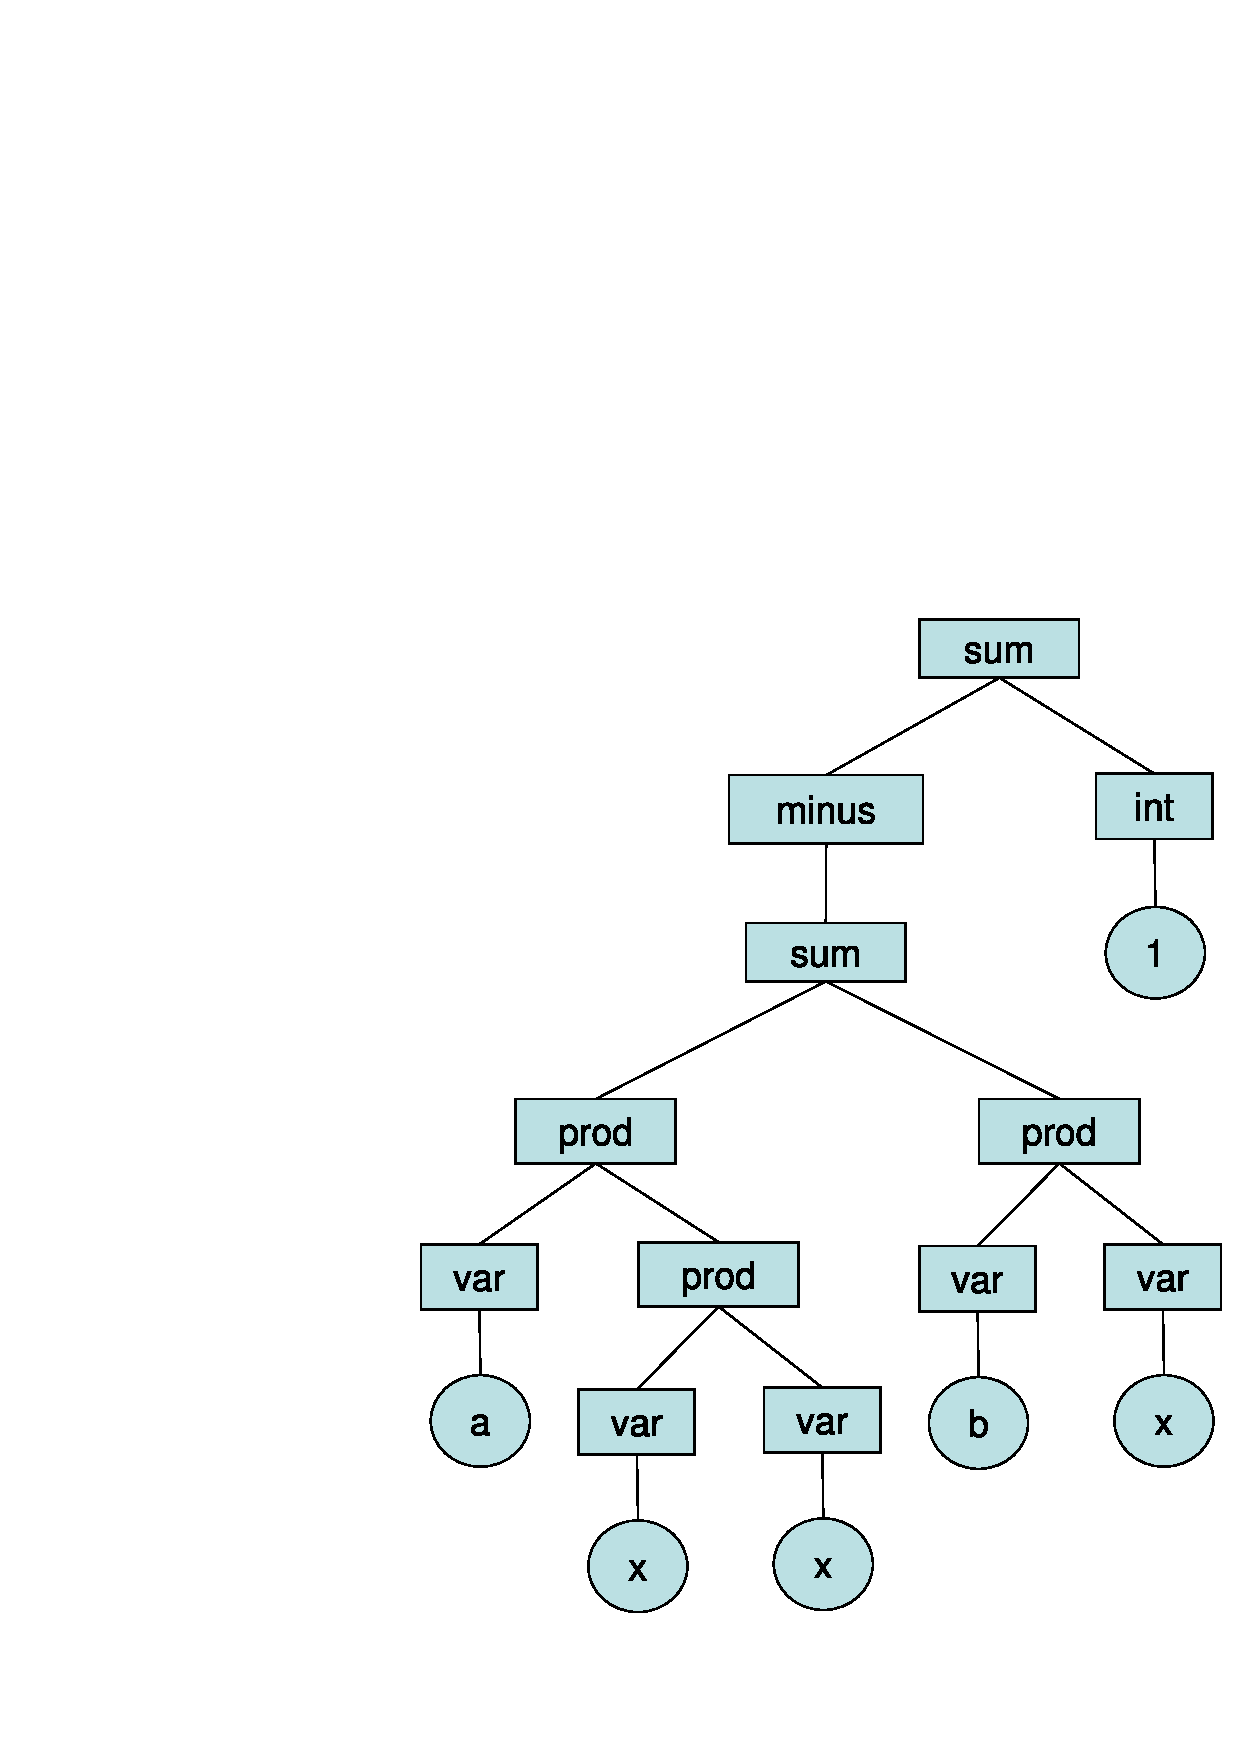
\includegraphics[height=4.5in]{figures/parsetree.pdf}
\caption{Parse tree for $-(a(x\cdot x)+ bx) + 1$.}
\label{fig:parse}
\end{figure}


Such a tree would be represented by pairs or triples that begin with a
\emph{tag} equal to the label of the top node of the parse tree.  We'll
call these tagged data items $\aexp$'s.  
\fi


\subsection{Evaluation and Substitution with Aexp's}

\subsubsection{Evaluating Aexp's}

Since the only variable in an \aexp\ is $x$, the value of an \aexp\ is
determined by the value of $x$.  For example, if the value of $x$ is 3,
then the value of $3x^2 + 2x + 1$ is obviously 34.  In general, given any
$\aexp$, $e$, and an integer value, $n$, for the variable, $x$, we can
evaluate $e$ to finds its value, $\meval(e,n)$.  It's easy, and useful, to
specify this evaluation process with a recursive definition.

\begin{definition}\label{meval-def}
  The \term{evaluation function}, $\meval: \aexp \times \integers \to
  \integers$, is defined recursively on expressions, $e \in \aexp$, as
  follows.  Let $n$ be any integer.

\begin{itemize}
\item \textbf{Base cases:}

\begin{enumerate}

\item\label{eval-var} Case[$e$ is $x$]
\[
\meval(x, n) \eqdef n.
\]
(The value of the variable, $x$, is given to be $n$.)

\item\label{eval-const} Case[$e$ is $\mtt{k}$]
\[
\meval(\mtt{k}, n) \eqdef k.
\]
(The value of the numeral $\mtt{k}$ is the integer $k$, no matter what
value $x$ has.)

\end{enumerate}

\item \textbf{Constructor cases:}

\begin{enumerate}
\setcounter{enumi}{2}

\item\label{eval-sum} Case[$e$ is $(e_1 \sumsym e_2)$]
\[
\meval((e_1 \sumsym e_2),n) \eqdef
  \meval(e_1,n)+\meval(e_2,n).
\]

\item\label{eval-prod} Case[$e$ is $(e_1 \prodsym e_2)$]
\[
\meval((e_1 \prodsym e_2),n) \eqdef \meval(e_1,n) \cdot \meval(e_2,n).
\]

\item\label{eval-minus} Case[$e$ is $\minussym(e_1)$]
\[
\meval(\minussym(e_1),n) \eqdef - \meval(e_1,n).
\]
\end{enumerate}

\end{itemize}

\end{definition}

For example, here's how the recursive definition of $\meval$ would arrive at
the value of $3+x^2$ when $x$ is 2:
\begin{align*}
\meval((\mtt{3} \sumsym (x \prodsym x)),2)
 & = \meval(\mtt{3},2) + \meval((x \prodsym x),2)
                  & \text{(by~Def~\ref{meval-def}.\ref{eval-sum})}\\
 & = 3 + \meval((x \prodsym x),2) & \text{(by~Def~\ref{meval-def}.\ref{eval-const})}\\
 & = 3 + (\meval(x,2) \cdot \meval(x,2)) & \text{(by~Def~\ref{meval-def}.\ref{eval-prod})}\\
 & = 3 + (2 \cdot 2) & \text{(by~Def~\ref{meval-def}.\ref{eval-var})}\\
 & = 3 + 4 = 7.
\end{align*}

\subsubsection{Substituting into Aexp's}
Substituting expressions for variables is a standard, important
operation.  For example the result of substituting the expression $3x$ for $x$
in the $(x(x-1))$ would be $(3x(3x-1)$.  We'll use the general
notation $\msubst{f}{e}$ for the the result of substituting an $\aexp$, $f$,
for each of the $x$'s in an $\aexp$, $e$.  For instance,
\[
\msubst{3x}{x(x-1)} = 3x(3x-1).
\]

This substitution function has a simple recursive definition:

\begin{definition}\label{subst-def}
  The \term{substitution function} from $\aexp \times \aexp$ to \aexp\ is
  defined recursively on expressions, $e \in \aexp$, as follows.  Let $f$
  be any $\aexp$.

\begin{itemize}
\item \textbf{Base cases:}

\begin{enumerate}

\item\label{subst-var} Case[$e$ is $x$]
\[
\msubst{f}{x} \eqdef f.
\]
(The result of substituting $f$ for the variable, $x$, is just $f$.)

\item\label{subst-const} Case[$e$ is $\mtt{k}$]
\[
\msubst{f}{\mtt{k}} \eqdef \mtt{k}.
\]
(The numeral, $\mtt{k}$, has no $x$'s in it to substitute for.)

\end{enumerate}

\item \textbf{Constructor cases:}

\begin{enumerate}
\setcounter{enumi}{2}
\item\label{subst-sum} Case[$e$ is $(e_1 \sumsym e_2)$]
\[
\msubst{f}{(e_1 \sumsym e_2)}) \eqdef  (\msubst{f}{e_1} \sumsym
\msubst{f}{e_2}).
\]

\item\label{subst-prod} Case[$e$ is $(e_1 \prodsym e_2)$]
\[
\msubst{f}{(e_1 \prodsym e_2)}) \eqdef  (\msubst{f}{e_1} \prodsym
\msubst{f}{e_2}).
\]

\item\label{subst-minus} Case[$e$ is $\minussym(e_1)$]
\[
\msubst{f}{\minussym(e_1)} \eqdef \minussym (\msubst{f}{e_1}).
\]

\end{enumerate}
\end{itemize}
\end{definition}

Here's how the recursive definition of the substitution function would find
the result of substituting $3x$ for $x$ in the $x(x-1)$:
\begin{align*}
\msubst{3x}{(x(x-1))} & =
\msubst{3x}{(x \prodsym (x \sumsym \minussym(1)))} & \text{(unabbreviating)}\\
 & = (\msubst{3x}{x} \prodsym \msubst{3x}{(x \sumsym \minussym(1))})
         & \text{(by~Def~\ref{subst-def}~\ref{subst-prod})}\\
 & = (3x \prodsym \msubst{3x}{(x \sumsym \minussym(1))})
         & \text{(by~Def~\ref{subst-def}~\ref{subst-var})}\\
 & = (3x \prodsym (\msubst{3x}{x} \sumsym \msubst{3x}{\minussym(1)}))
         & \text{(by~Def~\ref{subst-def}~\ref{subst-sum})}\\
 & = (3x \prodsym (3x \sumsym \minussym (\msubst{3x}{1})))
         & \text{(by~Def~\ref{subst-def}~\ref{subst-var} \&~\ref{subst-minus})}\\
 & = (3x \prodsym (3x \sumsym \minussym (1)))
         & \text{(by~Def~\ref{subst-def}~\ref{subst-const})}\\
 & = 3x(3x-1) & \text{(abbreviation)}
\end{align*}

Now suppose we have to find the value of $\msubst{3x}{(x(x-1))}$ when $x =
2$.  There are two approaches.

First, we could actually do the substitution above to get $3x(3x-1)$, and
then we could evaluate $3x(3x-1)$ when $x =2$, that is, we could
recursively calculate $\meval(3x(3x-1),2)$ to get the final value 30.  In
programming jargon, this would be called evaluation using the
\emph{Substitution Model}.  Tracing through the steps in the evaluation,
we find that the Substitution Model requires two substitutions for
occurrences of $x$ and 5 integer operations: 3 integer multiplications, 1
integer addition, and 1 integer negative operation.  Note that in this
Substitution Model the multiplication $3 \cdot 2$ was performed twice to
get the value of 6 for each of the two occurrences of $3x$.

The other approach is called evaluation using the \emph{Environment
  Model}.  Namely, we evaluate $3x$ when $x = 2$ using just 1
multiplication to get the value 6.  Then we evaluate $x(x-1)$ when $x$ has
this value 6 to arrive at the value $6\cdot 5=30$.  So the Environment
Model requires 2 variable lookups and only 4 integer operations: 1
multiplication to find the value of $3x$, another multiplication to find
the value $6 \cdot 5$, along with 1 integer addition and 1 integer
negative operation.

So the Environment Model approach of calculating
\[
\meval(x(x-1), \meval(3x,2))
\]
instead of the Substitution Model approach of calculating
\[
\meval(\msubst{3x}{x(x-1)},2)
\]
is faster.  But how do we know that these final values reached by these
two approaches always agree?  We can prove this easily by structural
induction on the definitions of the two approaches.  More precisely, what
we want to prove is

\begin{theorem}\label{environments}
For all expressions $e,f \in \aexp$ and $n \in \integers$,
\begin{equation}\label{eval-subst}
\meval(\msubst{f}{e},n) = \meval(e, \meval(f,n)).
\end{equation}
\end{theorem}

\begin{proof}
The proof is by structural induction on $e$.\footnote{This is an example
of why it's useful to notify the reader what the induction variable is
---in this case it isn't $n$.}

\textbf{Base cases:}
\begin{itemize}

\item Case[$e$ is $x$]

  The left hand side of equation~\eqref{eval-subst} equals $\meval(f,n)$
  by this base case in Definition~\ref{subst-def} of the substitution
  function, and the right hand side also equals $\meval(f,n)$ by this base
  case in Definition~\ref{meval-def} of $\meval$.


\item Case[$e$ is $\mtt{k}$].

  The left hand side of equation~\eqref{eval-subst} equals $\mtt{k}$ by
  this base case in Definitions~\ref{subst-def} and~\ref{meval-def} of
  the substitution and evaluation functions.  Likewise, the right hand
  side equals $\mtt{k}$ by two applications of this base case in the
  Definition~\ref{meval-def} of $\meval$.

\end{itemize}

\textbf{Constructor cases}:
\begin{itemize}

\item Case[$e$ is $(e_1 \sumsym e_2)$]

  By the structural induction hypothesis~\eqref{eval-subst}, we may assume
  that for all $f \in \aexp$ and $n \in \integers$,

\begin{equation}\label{ln4.hyp}
\meval(\msubst{f}{e_i},n)  =  \meval(e_i, \meval(f,n))
\end{equation}
for $i= 1,2$.  We wish to prove that

\begin{equation}\label{s+}
\meval(\msubst{f}{(e_1\sumsym e_2)},n)  =  \meval((e_1 \sumsym e_2), \meval(f,n))
\end{equation}

But the left hand side of~(\ref{s+}) equals
\[
\meval(\, (\msubst{f}{e_1} \sumsym \msubst{f}{e_2}),\ n)
\]
by Definition~\ref{subst-def}.\ref{subst-sum} of substitution into a sum
expression.  But this equals
\[
\meval(\msubst{f}{e_1},n) + \meval(\msubst{f}{e_2},n)
\]
by Definition~\ref{meval-def}.\ref{eval-sum} of $\meval$ for a sum expression.  By
induction hypothesis~\eqref{ln4.hyp}, this in turn equals
\[
\meval(e_1,\meval(f,n)) + \meval(e_2,\meval(f,n)).
\]
Finally, this last expression equals the right hand side of~(\ref{s+}) by
Definition~\ref{meval-def}.\ref{eval-sum} of $\meval$ for a sum
expression.  This proves~(\ref{s+}) in this case.

\item $e$ is $(e_1 \prodsym e_2)$.  Similar.

\item $e$ is $-(e_1)$.  Even easier.

\end{itemize}

This covers all the constructor cases, and so completes the proof by
structural induction.

\end{proof}


\iffalse
\subsection{A String Theorem}

Here is a more complex proof, illustrating a combination of structural
induction and strengthening the hypothesis.

\begin{theorem}
  In a string of $0$s and $1$s, the number of occurrences of the pattern
  $01$ is less than or equal to the number of occurrences of $10$, plus
  one.
\end{theorem}

Let's try to prove this by structural induction.  First we must
define $P(s)$.  Let's write $\ms{num}(pat,s)$ as the number of
occurrences of the pattern string pat in s.  Now our inductive
hypothesis is
\[
P(s): \ms{num}(01,s) \leq \ms{num}(10,s) + 1. 
\]
If you try to prove this by structural induction, you will get
stuck.
Why? 
Consider what happens when you add $1$ at the end.  
This could increase the number of $01$s without increasing the number of
$10$s. 

So, to prove by structural induction on strings, let's strengthen the
hypothesis by adding another clause.  If a string ends in $0$ then
the number of $01$s is less than or equal to the number of $10$s.
That solves the problem by weakening what we have to show when the
string ends in $1$.  But maybe it causes another problem somewhere
else.  Let's give it a try:

Redefine $P(s) \eqdef$
\begin{eqnarray*}
\ms{num}(01,s) & \leq & \ms{num}(10,s) + 1, \text{ and}\\
\leftenq{\text{If $s$ ends in $0$ then}}\\
\ms{num}(01,s) & \leq  &\ms{num}(10,s).
\end{eqnarray*} 
 
This means that, for each inductive step have two things to show.

\structuredproof{

  Prove: $\forall s \in S \; (P(s))$ \\
  1. (Base) $P(\emptystring)$ 
  \reason{No patterns of either kind.} \\
  2. (Inductive step) $\forall s \in S \; (P(s) \implies P(s 0))$ \\
  1. Fix $s$. \\
  2. Assume $P(s)$. \\
  3. $P(s 0)$ \\
  1. $\ms{num}(01,s0) \leq \ms{num}(10,s0) + 1$. 
  \reason{???} \\
  2. If $s 0$ ends in $0$ then $\ms{num}(01,s0) \leq
  \ms{num}(10,s0)$. \noreason \\
  \reason{???} \\
  3. QED
  \reason{Conjunction} \\
  4. QED 
  \reason{Implication, UG} \\
  3. (Inductive step) $\forall s \in S \; (P(s) \implies P(s 1))$ \\
  1. Fix $s$. \\
  2. Assume $P(s)$. \\
  3. $P(s 1)$ \\
  1. $\ms{num}(01,s1) \leq \ms{num}(10,s1) + 1$. 
  \reason{???} \\
  2. If $s 1$ ends in $0$ then $\ms{num}(01,s1) \leq
  \ms{num}(10,s1)$.\noreason \\
  \reason{???} \\
  3. QED
  \reason{Conjunction} \\
  4. QED 
  \reason{Implication, UG} \\
  4. QED
  \reason{Structural induction on strings.}\\
}

First let's consider $s1$. This is the case that looks dangerous,
because it might increase the number of $01$s.  We have to prove two
statements.  The second is easy, because the new string doesn't end in
$0$.  We say it's ``vacuously true''.

The first statement now takes some work. 
We might be adding to the number of $01$s.  
However, if we do, the previous string must have ended with $0$. 
Then the inductive hypothesis says that the previous string had to
satisfy the stronger inequality in the second statement. 
Adding one to the LHS of the stronger inequality yields the weaker
inequality we want.

The following proof fragment considers cases based on whether $s$ ends
in $0$ or not.  If not, it might end in $1$, or might be empty (don't
forget this possibility).

\begin{proof}
  3. $P(s 1)$ \\
  1. $\ms{num}(01,s1) \leq \ms{num}(10,s1) + 1$. \\
  1. If $s$ ends in $0$ then $\ms{num}(01,s1) \leq\ms{num}(10,s1) + 1$. \\
  1. Assume $s$ ends in $0$. \\
  2. $\ms{num}(01,s) \leq \ms{num}(10,s)$ 
  Inductive hypothesis (3.2), part 2. \\
  3. $\ms{num}(01,s1) = \ms{num}(01,s) + 1$ 
  Adding one more $01$. \\
  4. $\ms{num}(10,s1) = \ms{num}(10,s)$ \\
  5. $\ms{num}(01,s1) \leq\ms{num}(10,s1) + 1$. 
  Algebra (combining 3.3.1.1.2, ...3, and ...4) \\
  QED 
  Implication \\
  2. If $s$ ends in $1$ then $\ms{num}(01,s1)\leq\ms{num}(10,s1) + 1$. \\
  Inductive hypothesis, part 1; no new $01$s. \\
  3. If $s = \emptystring$ then $\ms{num}(01,s1) \leq\ms{num}(10,s1)+ 1$. \\
  $s1$ is just $1$, which has no $01$s. \\
  4. QED 
  Cases \\
  2. If $s 1$ ends in $0$ then $\ms{num}(01,s1) \leq \ms{num}(10,s1)$. \\
  Vacuously true, because $s1$ doesn't end in $0$. \\
  3. QED
  Conjunction \\
\end{proof}
Of course, you could also expand the step for $s$ ending in $1$ into a
careful series of inequalities.

Now consider $s0$.  We hope that what we did to make the $s1$ case
work doesn't mess up the $s0$ case.  But we have to check.

The first statement is easy.  It follows from the first statement of
the inductive hypothesis for $s$, because we are not increasing the
number of $01$s.  But now the second statement takes more work.  The
difficulty is that the new string ends in $0$, which means that we
have to show the stronger inequality in the second statement.  But to
do this, we might only have the weaker inequality for the previous
string.  The argument again depends on what the previous string $s$
ended with.  So again, we consider cases, based on whether $s$ ends in
$0$ or $1$, or is empty.  If $s$ ends in $0$ we rely on the second
statement of the inductive hypothesis for $s$ (with the stronger
inequality), whereas if $s$ ends in $1$ we rely on the first statement
(with the weaker inequality).  In this case, we have to ``turn the
weaker inequality into the stronger inequality''.

\structuredproof[38ex]{
  3. $P(s 0)$ \\
  1. $\ms{num}(01,s0) \leq \ms{num}(10,s0) + 1$.
  \reason{Induct. hypothesis, part 1; no new $01$s.} \\
  2. If $s 0$ ends in $0$ then $\ms{num}(01,s0) \leq\ms{num}(10,s0)$. \\
  1. $\ms{num}(01,s0) \leq \ms{num}(10,s0)$. \\
  1. If $s$ ends in $0$ then $\ms{num}(01,s0)
  \leq\ms{num}(10,s0)$. \noreason \\
  \reason{Induct. hypothesis, part 2; no new $01$s} \\
  2. If $s$ ends in $1$ then $\ms{num}(01,s0)
  \leq\ms{num}(10,s0)$. \noreason \\ 
  1. Assume $s$ ends in $1$. \\
  2. $\ms{num}(01,s) \leq \ms{num}(10,s) + 1$. 
  \reason{Inductive hypothesis, part 1} \\
  3. $\ms{num}(01,s0) = \ms{num}(01,s)$ \\
  4. $\ms{num}(10,s0) = \ms{num}(10,s) + 1$ 
  \reason{Exactly one new occurrence of $10$.} \\
  5. $\ms{num}(01,s0) \leq \ms{num}(10,s0)$ 
  \reason{Algebra} \\
  6. QED
  \reason{Implication} \\
  3. If $s = \emptystring$ then $\ms{num}(01,s0) \leq
  \ms{num}(10,s0)$. \noreason \\ 
  
\reason{$s0$ is just $1$, which has no $01$s or $10$s.} \\
  4. QED 
  \reason{Cases} \\
  2. QED
  \reason{Propositional reasoning (truth table)} \\
  3. QED 
  \reason{Conjunction}\\
}

If you actually write out all these cases in the proof, you will
notice that some facts are stated repeatedly, e.g., that when you add
a $0$ to the end of a string you are not increasing the number of
$01$s.  To avoid having to state these facts several times, you can
move them earlier in the proof.
\fi


\iffalse

\begin{example*}
\begin{definition}\label{E}
Define a set, $E$, recursively as follows:
\begin{itemize}
\item \textbf{Base case:} $0 \in E$,\label{0E}
\item \textbf{Constructor cases:} if $n \in E$, then
\begin{enumerate}
\item $n+2 \in E$, when $n\geq 0$;\label{+2E}
\item $-n \in E$, when $n > 0$.\label{-E}
\end{enumerate}
\end{itemize}

\end{definition}
\end{example*}

Using this definition, we can see that $0 \in E$ by the Base case, so $0 +
2 = 2 \in E$ by Constructor case~\ref{+2E}., and so $2+2 =4 \in E$, $4+2 =
6 \in E$, \dots, and in fact any nonnegative even number is in $E$ by
successive application of case~\ref{+2E}.  Also, by case~\ref{-E}.,
$-2,-4,-6,\dots \in E$.  So clearly all the even integers are in $E$.

Is anything else in $E$?  The definition doesn't say so explicitly, but an
implicit condition on a recursive definition is that the only way things
get into $E$ is as a consequence of the Base and Constructor cases.  In
other words, $E$ will be exactly the set of even integers.

A very simple application of structural induction proves that the set $E$
given by Definition~\ref{E} is exactly the set of even numbers.  We already
explained why all the even numbers are in $E$.  So what's left is to show
that:

\begin{lemma*}
Every number in the set $E$ in Definition~\ref{E} is even.
\begin{proof}
The proof is by structural induction on $n \in E$.  The induction
hypothesis is 
\[
Q(n) \eqdef \text{$n$ is even}.
\]

\textbf{Base case}: $Q(0)$ holds since 0 is even.

\textbf{Constructor cases}: assuming $n \in E$ and $Q(n)$ holds, prove
that
\begin{itemize}

\item $Q(n+2)$ holds.  This is immediate, since adding 2 to an even number
  gives an even number.

\item $Q(-n)$ holds.  This is also immediate, since $n$ is even iff $-n$ is
even.

\end{itemize}

This completes the proof of the Constructor cases, and we conclude by
structural induction at $Q(n)$ holds for all $n \in E$.
\end{proof}

\end{lemma*}


defining the set, $E$, of even numbers as in Definitions~\ref{E}, but
without the conditions~\ref{+2E}.\ and~\ref{-E}.\ that restrict application of
the rules.  Namely,

\begin{definition}\label{Eamb}
Define a set, $E'$, recursively as follows:
\begin{itemize}
\item \textbf{Base case:} $0 \in E'$,\label{0Eamb}
\item \textbf{Constructor cases:} if $n \in E'$, then
\begin{enumerate}
\item $n+2 \in E'$, \label{+2Eamb}
\item $-n \in E'$.\label{-Eamb}
\end{enumerate}
\end{itemize}
\end{definition}

Now Definition~\ref{Eamb} is perfectly legitimate, and we could us it to
prove by structural induction that $E'$ also is the set of even integers,
that is, $E'= E$.  But Definition~\ref{Eamb} is ambiguous.  For example,
$0\in E'$ by the base case, but also $0=-0 \in E'$ by applying constructor
case~\ref{-Eamb} to the base case.  This begins to matter when we try to
define a function, $s$, from $E'$ to nonnegative integers based on
Definition~\ref{Eamb}:
\begin{align*}
  s(0) & \eqdef 1,\\
s(n+2) & \eqdef 1+ s(n),\\
 s(-n) & \eqdef 1+ s(n).
\end{align*}
So $s(0) \eqdef 1$ by the base case of this definition, and also $s(0)=
s(-0) \eqdef 1+s(0) = 1 + 1 = 2$ by the second constructor case, which
shows that these rules are inconsistent.

On the other hand, using the unambiguous Definition~\ref{E} of $E$,
essentially the same definition of $S$ works just fine.  Namely, define
\begin{align*}
  s(0) & \eqdef 1,\\
  s(n+2) & \eqdef 1+ s(n), & \text{ for } n \geq 0\\
  s(-n) & \eqdef 1+ s(n) & \text{ for } n > 0.
\end{align*}
Now $s(n)$ is unambiguously defined, and in fact is precisely the (unique)
number of steps required to construct $n \in E$ according to the
unambiguous Definition~\ref{E} of $E$.
\fi


%% Structural Induction on Recursive Data Types
%% Problems %%%%%%%%%%%%%%%%%%%%%%
\begin{problems}
\classproblems
\pinput{CP_F18_functions}
\pinput{CP_recursively_defined_sets}
\pinput{CP_erasable_strings}
\pinput{CP_binary_trees}

\homeworkproblems
\pinput{PS_bracket_good_count}
\pinput{PS_koch_snowflake}

\end{problems}

%% Games as a Recursive Data Type %%%%%%%%%%%%%%%%%%%%%%%%%%%%%%%%%%%%%%%%%%%%%
\section{Games as a Recursive Data Type}

Chess, Checkers, and Tic-Tac-Toe are examples of \emph{two-person
terminating games of perfect information}, ---$\tg$'s for short.  These
are games in which two players alternate moves that depend only on the
visible board position or state of the game.  ``Perfect information''
means that the players know the complete state of the game at each move.
(Most card games are \emph{not} games of perfect information because
neither player can see the other's hand.)  ``Terminating'' means that play
cannot go on forever ---it must end after a finite number of
moves.\footnote{Since board positions can repeat in chess and checkers,
termination is enforced by rules that prevent any position from being
repeated more than a fixed number of times.  So the ``state'' of these
games is the board position \emph{plus} a record of how many times
positions have been reached.}

We will define $\tg$'s \iffalse in a straightforward way tagged\fi as a 
recursive data type.  To see how this will work, let's use the game of
Tic-Tac-Toe as an example.

\subsection{Tic-Tac-Toe}

Tic-Tac-Toe is a game for young children.  There are two players who
alternately write the letters ``X'' and ``O'' in the empty boxes of a $3
\times 3$ grid.  Three copies of the same letter filling a row, column, or
diagonal of the grid is called a \emph{tic-tac-toe}, and the first player
who gets a tic-tac-toe of their letter wins the game.  \iffalse Children
generally don't take long to figure out an optimal strategy for playing the
game.\fi


We're now going give a precise mathematical definition of the Tic-Tac-Toe
\term{game tree} as a recursive data type.  \iffalse and carefully defining
the allowed moves Children of course have no need for such a definition,
and it would be too complicated for them anyway.  But if we had to write a
Tic-Tac-Toe playing \emph{computer program}, we'd need this kind of picky
precision.\fi Here's the idea behind the definition: at any point in the
game, the ``board position'' is the pattern of X's and O's on the $3 \times
3$ grid.  From any such Tic-Tac-Toe pattern, there are a number of next
patterns that might result from a move.  For example, from the initial
empty grid, there are nine possible next patterns, each with a single X in
some grid cell and the other eight cells empty.  From any of these
patterns, there are eight possible next patterns gotten by placing an O in
an empty cell.  These move possibilities are given by the
\hyperdef{game}{tree}{game tree} for Tic-Tac-Toe indicated in
Figure~\ref{fig:Tic-Tac-Toe}.

\begin{figure}[htbp]
\centering
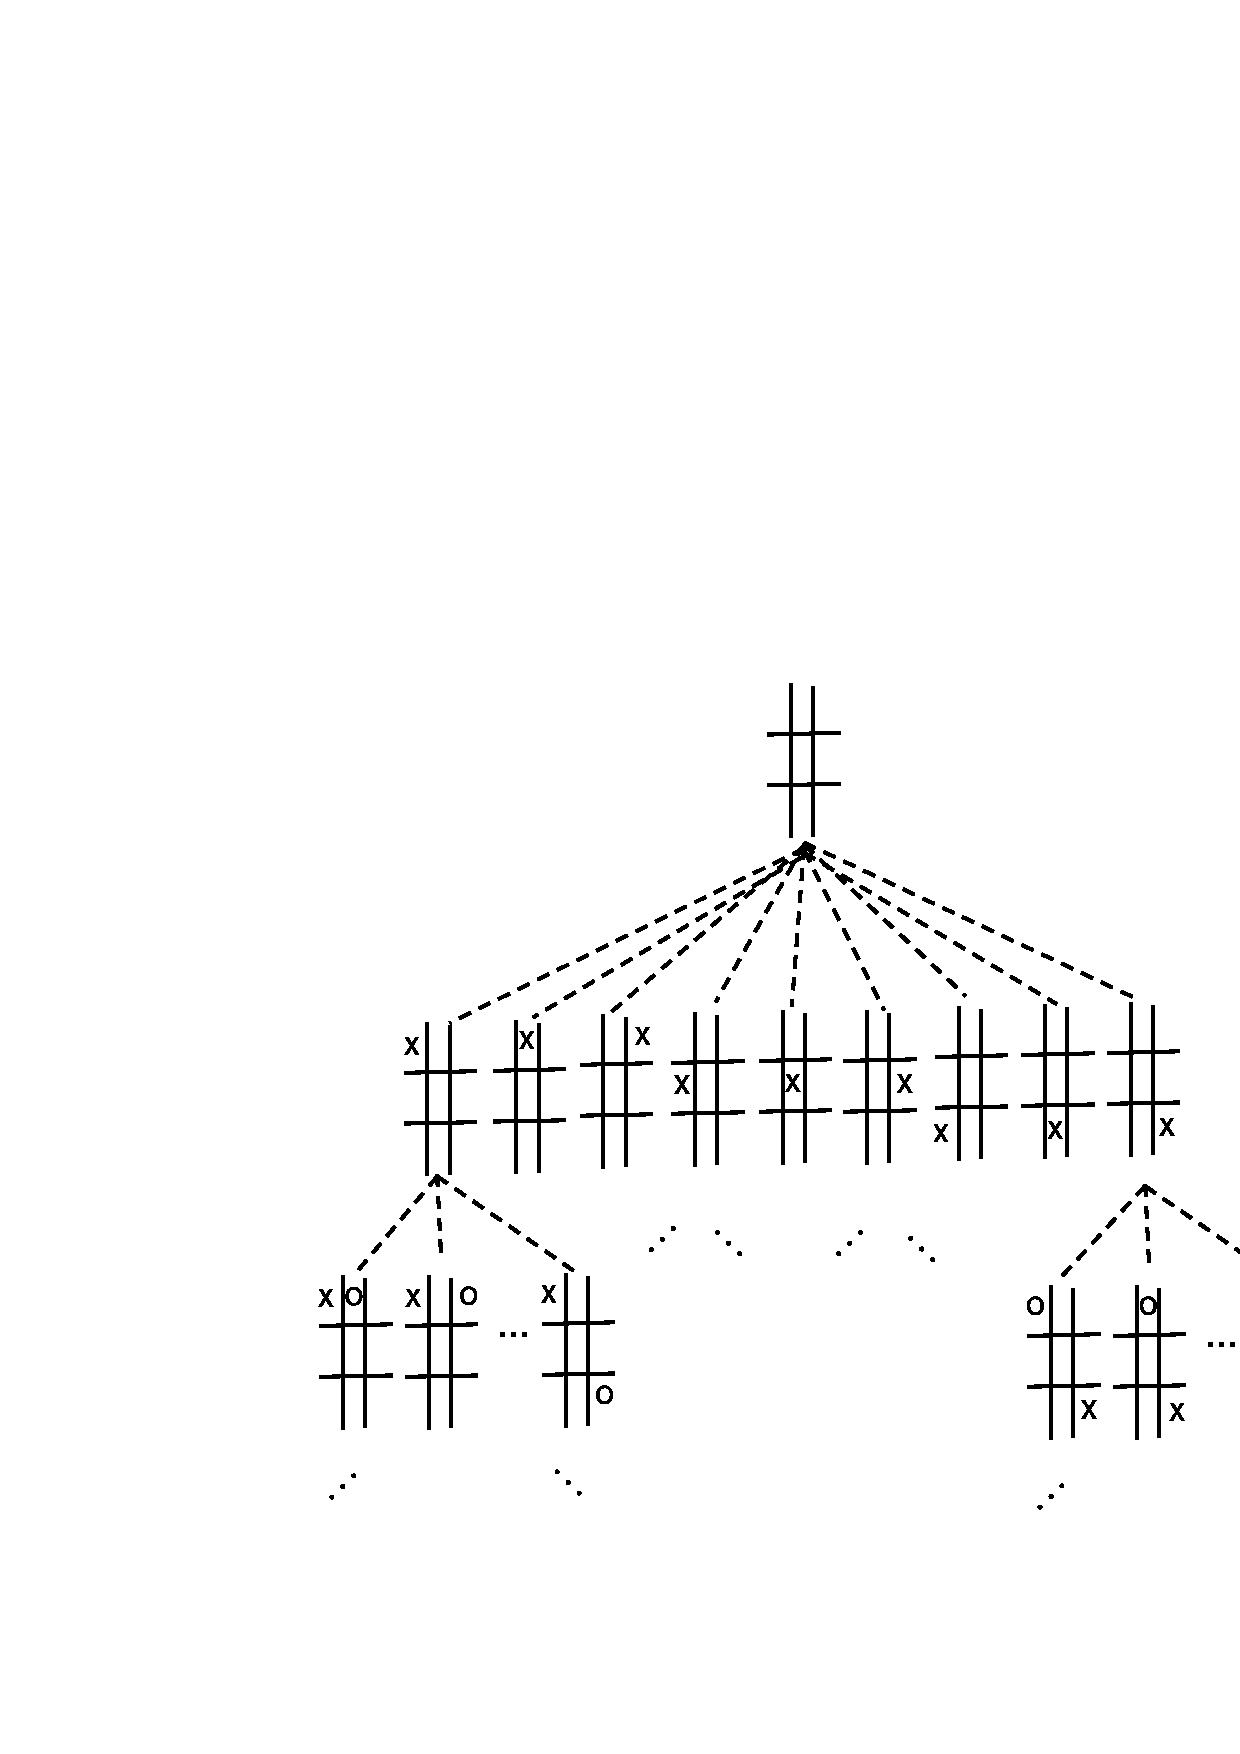
\includegraphics[height=6in]{figures/topgame.pdf}
\caption{The Top of the Game Tree for Tic-Tac-Toe.}
\label{fig:Tic-Tac-Toe}
\end{figure}


\iffalse
\[\begin{array}{c|c|c}
\hspace{.1in} & \hspace{.1in} & \hspace{.1in}\\
\hline  & &\\
\hline  & &
\end{array}\]

\textbf{FIGURE NEEDED}
\fi

\begin{definition}

A Tic-Tac-Toe \emph{pattern} is a $3 \times 3$ grid each of whose 9 cells
contains either the single letter, X, the single letter, O, or is
empty.
\iffalse
Moreover, there must be either
\begin{itemize}

\item one more X than O's, with at most two tic-tac-toes of X's, and no
tic-tac-toe of O's, or

\item an equal number of X's and O's, with at most one tic-tac-toes of
O's, and no tic-tac-toe of X's.
\end{itemize}
\fi

A pattern, $Q$, is a \emph{possible next pattern after} $P$, providing $P$
has no tic-tac-toes and
\begin{itemize}

\item if $P$ has an equal number of X's and O's, and $Q$ is the same as
$P$ except that a cell that was empty in $P$ has an X in $Q$, or

\item if $P$ has one more X than O's, and $Q$ is the same as $P$ except
that a cell that was empty in $P$ has an O in $Q$.
\end{itemize}

If $P$ is a Tic-Tac-Toe pattern, and $P$ has no next patterns, then the
\emph{terminated Tic-Tac-Toe game trees} at $P$ are

\begin{itemize}

\item 
\[
\ang{P, \ang{\texttt{win}}},
\]
if $P$ has a tic-tac-toe of X's.


\item 
\[
\ang{P, \ang{\texttt{lose}}},
\]
if $P$ has a tic-tac-toe of O's.


\item
\[
\ang{P, \ang{\texttt{tie}}},
\]
otherwise.

\end{itemize}


\iffalse
If $Q$ is a possible move from $P$, then the game tree starting at $Q$ is
called a \emph{  Notice
that $\mathcal{G}_P = \emptyset$ iff $P$ is terminated.}
\fi

The \emph{Tic-Tac-Toe game trees starting at $P$} are defined recursively:

\textbf{Base Case}:
A terminated Tic-Tac-Toe game tree at $P$ is a Tic-Tac-Toe game tree
starting at $P$.

\textbf{Constructor case}: If $P$ is a non-terminated Tic-Tac-Toe pattern,
then the Tic-Tac-Toe game tree starting at $P$ consists of $P$ and the set
of all game trees starting at possible next patterns after $P$.
\end{definition}

For example, if
\begin{align*}
P_0 & =  \begin{array}{c|c|c}
                O & X & O\\
         \hline X & O & X\\
         \hline X & &
        \end{array}\\
Q_1 & = \begin{array}{c|c|c}
                O & X & O\\
         \hline X & O & X\\
         \hline X &  & O
        \end{array}\\
Q_2 & = \begin{array}{c|c|c}
                O & X & O\\
         \hline X & O & X\\
         \hline X & O & 
        \end{array}\\
R & = \begin{array}{c|c|c}
                O & X & O\\
         \hline X & O & X\\
         \hline X & O & X
        \end{array}
\end{align*}
the game tree starting at $P_0$ is pictured in Figure~\ref{fig:endgame}.

\iffalse
Then,
\begin{equation}\label{endgame}
\ang{P, \set{\ang{Q_1, \ang{\texttt{lose}}},
             \ang{Q_2, \set{\ang{R,\ang{\texttt{tie}}}}}}}
\end{equation}
is the tagged recursive datum that corresponds to a Tic-Tac-Toe ``end
game'' that starts with $P$.  This game is easier to understand by looking
at its game tree in Figure~\ref{fig:endgame}.  Notice that the game tree
---which so far we haven't actually defined ---is simply the parse tree of
the tagged datum.\fi


\begin{figure}[htbp]
\centering
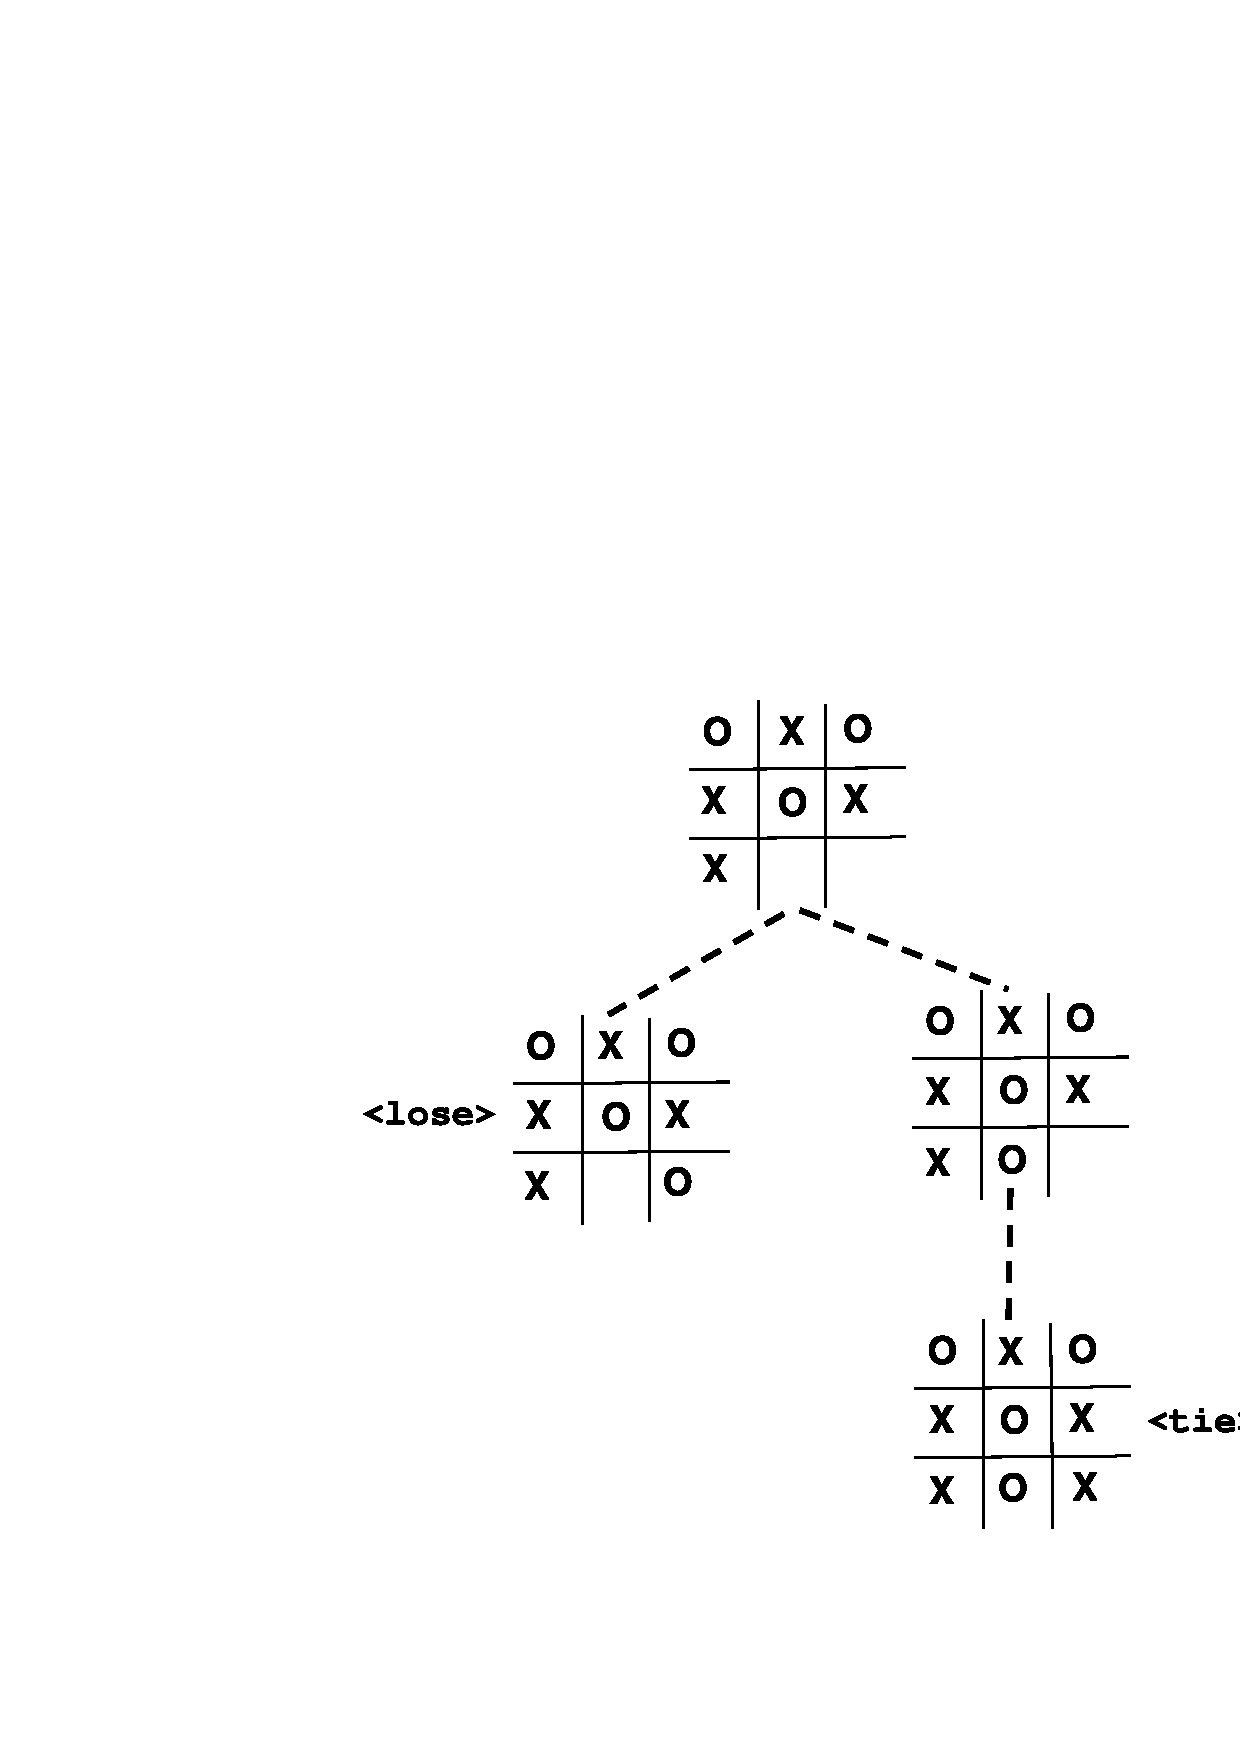
\includegraphics[height=4in]{figures/endgame.pdf}
\caption{Game Tree for the Tic-Tac-Toe game starting at $P_0$.}
\label{fig:endgame}
\end{figure}

Game trees are usually pictured in this way with the starting pattern
(referred to as the ``root'' of the tree) at the top and lines connecting
the root to the \iffalse roots of the \fi game trees that start at each
possible next pattern.  The ``leaves'' at the bottom of the tree (trees
grow upside down in computer science) correspond to terminated games.  A
path from the root to a leaf describes a complete \emph{play} of the game.
(In English, ``game'' can be used in two senses: first we can say that
Chess is a game, and second we can play a game of Chess.  The first usage
refers to the data type of Chess game trees, and the second usage refers to
a ``play.'')

\subsection{Infinite Tic-Tac-Toe Games}

At any point in a Tic-Tac-Toe game, there are at most nine possible
next patterns, and no play can continue for more than nine moves.  But
we can expand Tic-Tac-Toe into a larger game by running a 5-game
tournament: play Tic-Tac-Toe five times and the tournament winner is
the player who wins the most individual games.  A 5-game tournament
can now run for as many as 45 moves.

Now it's not much of generalization to have an \emph{$n$-game
Tic-Tac-Toe tournament}.  But now there's a generalization that sounds
simple but can be mind-bogging: consolidate all these different size
tournaments into a single game we can call
\emph{Tournament-Tic-Tac-Toe ($T^4$)}.  The first player in a game of $T^4$
chooses any integer $n > 0$.  Then the players play an $n$-game
tournament.  Now we can no longer say how long a $T^4$ play can take.
In fact, there are $T^4$ plays that last as long as you might like: of
you want a game that has a play with, say, nine billion moves, just
have the first play choose $n$ equal to one billion.  This should make
it clear the game tree for $T^4$ is infinite.

But still, it's obvious that every possible $T^4$ play will stop.
That's because after the first player chooses a value for $n$, the
game can't continue for more than $9n$ moves.  So it's not possible to
keep playing forever even though the game tree is infinite.

This isn't very hard to understand, but there is an important
difference between any given $n$-game tournament and $T^4$: even
though every play of $T^4$ must come to an end, there is no longer any
initial bound on how many moves it might be before the game ends ---a
play might end after 9 moves, or $9(2001)$ moves, or $9(10^{10}+1)$
moves.  It just can't continue forever.

\iffalse While there is no bound on how long to play, at least after the
first move to an $n \times n$ board in meta-Tic-Tac-Toe, we know the game
will end with $n^2$ moves.\fi

Now that we recognize $T^4$ as a \tg, we can go on to
a \emph{meta}-$T^4$ game, where the first player chooses a number,
$m>0$, of $T^4$ games to play, and then the second player gets the
first move in each of the individual $T^4$ games to be played.

Then, of course, there's meta-meta-$T^4$\dots.

\iffalse Every play of the meta-meta game must still end, but now even
after the first move, there is no bound on how long a game might
continue.\fi

\subsection{Two Person Terminating Games}

Familiar games like Tic-Tac-Toe, Checkers, and Chess can all end in
ties, but for simplicity we'll only consider win/lose games ---no
``everybody wins''-type games at MIT. \texttt{:-)}.  But everything we
show about win/lose games will extend easily to games with ties, and
more generally to games with outcomes that have different payoffs.

\iffalse
Of course Tic-Tac-Toe and the
other games will fit this set up if we treat a game that ends in a tie as
a loss for the usual first player ---White in Chess, Red in Checkers, the
X-player in Tic-Tac-Toe.
\fi

Like Tic-Tac-Toe, or Tournament-Tic-Tac-Toe, the idea behind the
definition of $\tg$'s as a recursive data type is that making a move
in a $\tg$ leads to the start of a subgame.  In other words, given any
set of games, we can make a new game whose first move is to pick a
game to play from the set.

So what defines a game?  For Tic-Tac-Toe, we used the patterns and the
rules of Tic-Tac-Toe to determine the next patterns.  But once we have
a complete game tree, we don't really need the pattern labels: the
root of a game tree itself can play the role of a ``board position''
with its possible ``next positions'' determined by the roots of its
subtrees.  So any game is defined by its game tree.  This leads to the
following very simple ---perhaps deceptively simple ---general
definition.

\begin{definition}
The \hyperdef{2p}{tg}{$\tg$}, \emph{game trees for two-person terminating
    games of perfect information} are defined recursively as follows:
\begin{itemize}

\item \textbf{Base cases:}
\[\begin{array}{ll}
\ang{\texttt{leaf},\texttt{win}} & \in \tg, \text{ and}\\
\ang{\texttt{leaf},\texttt{lose}}& \in \tg.
\end{array}\]

\item \textbf{Constructor case:}
If $\mathcal{G}$ is a nonempty set of
$\tg$'s, then $G$ is a $\tg$, where
\[
G \eqdef \ang{\texttt{tree},\mathcal{G}}.
\]
The game trees in $\mathcal{G}$ are called the possible \emph{next moves}
from $G$.
\end{itemize}

\end{definition}

These games are called ``terminating'' because, even though a $\tg$ may be
a (very) infinite datum like Tournament$^2$-Tic-Tac-Toe, every play of a
$\tg$ must terminate.  This is something we can now prove, after we give a
precise definition of ``play'':

\begin{definition}
A \emph{play} of a $\tg$, $G$, is a (potentially infinite) sequence of
$\tg$'s starting with $G$ and such that if $G_1$ and $G_2$ are consecutive
$\tg$'s in the play, then $G_2$ is a possible next move of $G_1$.

If a $\tg$ has no infinite play, it is called a \emph{terminating} game.
\end{definition}

\begin{theorem}
Every $\tg$ is terminating.
\end{theorem}

\begin{proof}
By structural induction on the definition of a $\tg$, $G$, with induction
hypothesis
\[
G \text{ is terminating}.
\]

\textbf{Base case}: If $G = \ang{\texttt{leaf}, \texttt{win}}$ or $G =
\ang{\texttt{leaf}, \texttt{lose}}$ then the only possible play of $G$ is
the length one sequence consisting of $G$.  Hence $G$ terminates.

\textbf{Constructor case}: For $G = \ang{\texttt{tree},\mathcal{G}}$, we
must show that $G$ is terminating, given the Induction Hypothesis that
\emph{every} $G' \in \mathcal{G}$ is terminating.

But any play of $G$ is, by definition, a sequence starting with $G$ and
followed by a play starting with some $G_0 \in \mathcal{G}$.  But $G_0$ is
terminating, so the play starting at $G_0$ is finite, and hence so is the
play starting at $G$.

This completes the structural induction, proving that every \tg, $G$, is
terminating.
\end{proof}


\subsection{Game Strategies}

A key question about a game is whether a player has a winning strategy.  A
\emph{strategy} for a player in a game specifies which move the player
should make at any point in the game.  A \emph{winning} strategy ensures
that the player will win no matter what moves the other player makes.

In Tic-Tac-Toe for example, most elementary school children figure out
strategies for both players that each ensure that the game ends with no
tic-tac-toes, that is, it ends in a tie.  Of course the first player can
win if his opponent plays childishly, but not if the second player follows
the proper strategy.  In more complicated games like Checkers or Chess,
it's not immediately clear that anyone has a winning strategy, even if we
agreed to count ties as wins for the second player.

But structural induction makes it easy to prove that in any $\tg$,
\emph{somebody} has the winning strategy!

\begin{theorem}\label{fund}
\textbf{Fundamental Theorem for Two-Person Games:} For every two-person
terminating game of perfect information, there is a winning strategy for
one of the players.
\end{theorem}

\begin{proof}
The proof is by structural induction on the definition of a $\tg$, $G$.
The induction hypothesis is that there is a winning strategy for $G$.

\textbf{Base cases:}
\begin{enumerate}

\item $G=\ang{\texttt{leaf}, \texttt{win}}$.  Then the first player has the
 winning strategy: ``make the winning move.''

\item $G=\ang{\texttt{leaf}, \texttt{lose}}$.  Then the second player has a
 winning strategy: ``Let the first player make the losing move.''
\end{enumerate}

\textbf{Constructor case}: Suppose $G = \ang{\texttt{tree},\mathcal{G}}$.
By structural induction, we may assume that some player has a winning
strategy for each $G' \in \mathcal{G}$.  There are two cases to consider:
\begin{itemize}
\item some $G_0 \in \mathcal{G}$ has a winning strategy for its second
  player.  Then the first player in $G$ has a winning strategy: make the
  move to $G_0$ and then follow the second player's winning strategy in
  $G_0$.

\item every $G' \in \mathcal{G}$ has a winning strategy for its first
  player.  Then the second player in $G$ has a winning strategy: if the
  first player's move in $G$ is to $G_0 \in \mathcal{G}$, then follow the
  winning strategy for the first player in $G_0$.
\end{itemize}
So in any case, one of the players has a winning strategy for $G$, which
completes the proof of the constructor case.

It follows by structural induction that there is a winning strategy for
every $\tg$, $G$.
\end{proof}

Notice that although Theorem~\ref{fund} guarantees a winning strategy, its
proof gives no clue which player has it.  For
\iffalse the Subset Takeaway Game
(\href{http://courses.csail.mit.edu/6.042/fall07/rec3t.pdf} {Recitation
Problem, Tuesday, Week 3}), and
\fi
most familiar $\tg$'s like Chess, Go, \dots, no one knows
which player has a winning strategy.\footnote{Checkers used to be in this
  list, but there has been a recent announcement that each player has a
  strategy that forces a tie. (reference TBA)}

%% Games as a Recursive Data Type Problems %%%%%%%%%%%%%%%%%%%%%%%%%%%%%%%%%%%%
%\startclassproblems

\begin{problems}
%\classproblems
\homeworkproblems
\pinput{PS_50_point_games}
\end{problems}

%% Induction in Computer Science %%%%%%%%%%%%%%%%%%%%%%%%%%%%%%%%%%%%%%%%%%%%%%
\section{Induction in Computer Science}

Induction is a powerful and widely applicable proof technique, which is why
we've devoted an entire chapter to it.  Strong induction and its special
case of ordinary induction are applicable to any kind of thing with
nonnegative integer sizes --which is a awful lot of things, including all
step-by-step computational processes.

\iffalse
Ordinary induction is specially helpful in the study of computation.  Why?
Well, ordinary induction on nonnegative integers is a ``one step at a
time'' proof method.  Computations also evolve ``one step at a time.''
\fi

Structural induction then goes beyond natural number counting by offering a
simple, natural approach to proving things about recursive computation
and recursive data types.  This makes it a technique every computer
scientist should embrace.

\iffalse
In many cases a nonnegative integer size can be defined for a recursively
defined datum, such as the length of a string, or the number of operations
in an $\aexp$.  It is then possible to prove properties of data by ordinary
induction on their size.  But this approach often produces more cumbersome
proofs than structural induction.

In fact, structural induction is theoretically more powerful than ordinary
induction.  However, it's only more powerful when it comes to reasoning
about infinite data types ---like infinite trees, for example ---so this
greater power doesn't matter in practice.  What does matter is that for
recursively defined data types, structural induction is a simple and
natural approach.
\fi

\endinput
 %structural induction, Ackermann function, while
                         %programs, games  *Albert
%%% Jay: there is some commented out material in ln3 about games wrt PO's

\chapter{Planar Graphs}\label{planar_graphs_chap}

\section{Drawing Graphs in the Plane}

Suppose there are three dog houses and three human houses, as shown in
Figure~\ref{fig:5DP}.  Can you find a route from each dog house to
each human house such that no route crosses any other route?

\begin{figure}

\graphic{dog-houses}

\caption{Three dog houses and and three human houses.  Is there a
  route from each dog house to each human house so that no pair of
  routes cross each other?}
\label{fig:5DP}
\end{figure}

A similar question comes up about a little-known animal called a
\emph{quadrapus} that looks like an octopus with four stretchy arms
instead of eight.  If five quadrapi are resting on the sea floor, as shown
in Figure~\ref{fig:5DA}, can each quadrapus simultaneously shake hands
with every other in such a way that no arms cross?

\begin{figure}

\graphic{quadrapi}

\caption{Five quadrapi (4-armed creatures).}

\label{fig:5DA}

\end{figure}


\begin{editingnotes}
\textcolor{red}{rephrased by ARM 7/3/10:}
\end{editingnotes}

Both these puzzles can be understood as asking about drawing graphs in the
plane.  Replacing dogs and houses by nodes, the dog house puzzle can be
rephrased as asking whether there is a planar drawing of the graph with
six nodes and edges between each of the first three nodes and each of the
second three nodes.  This graph is called the \term{complete bipartite
  graph} \idx{$K_{3,3}$} and is shown in Figure~\ref{fig:nonplanar}.(a).
\begin{editingnotes}
Insert graphic and fix figure refs.
\end{editingnotes}
The quadrapi puzzle asks whether there is a planar drawing of the
\idx{complete graph} \idx{$K_5$} shown in
Figure~\ref{fig:nonplanar}.(b).

\begin{figure}

\subfloat[]{%
    \graphic{Fig_5_36a}
}
\qquad\qquad
\subfloat[]{%
    \graphic{Fig_5_36b}
}

\caption{$K_{3, 3}$ (a) and $K_5$ (b).  Can you redraw these graphs so
that no pairs of edges cross?}

\label{fig:nonplanar}

\end{figure}

In each case, the answer is, ``No ---but almost!''  In fact, if you
remove an edge from either of these graphs, then the resulting graph
\emph{can} be redrawn in the plane so that no edges cross, as shown in
Figure~\ref{fig:5DC}.


\begin{figure}

\subfloat[]{
    \graphic{Fig_5DC_a}
}
\qquad
\subfloat[]{
    \graphic{Fig_5DC_b}
}

\caption{Planar drawings of (a) $K_{3, 3}$ without $\edge{u}{v}$, and
  (b) $K_5$ without $\edge{u}{v}$.}
\label{fig:5DC}
\end{figure}

Planar drawings have applications in circuit layout and are helpful in
displaying graphical data such as program flow charts, organizational
charts, and scheduling conflicts.  For these applications, the goal is
to draw the graph in the plane with as few edge crossings as possible.
(See the box on the following page for one such example.)

\begin{figure}[p]\redrawntrue
\textbox{\textboxtitle{Steve Wozniak and a Planar Circuit Design}

\noindent
When wires are arranged on a surface, like a circuit board or
microchip, crossings require troublesome three-dimensional structures.
When Steve Wozniak designed the disk drive for the early Apple II
computer, he struggled mightily to achieve a nearly planar design
according to the following excerpt from \texttt{apple2history.org}
which in turn quotes \emph{Fire in the Valley} by Freiberger and
Swaine:

\begin{quotation}
\noindent For two weeks, he worked late each night to make a satisfactory
design.  When he was finished, he found that if he moved a connector he
could cut down on feedthroughs, making the board more reliable.  To make
that move, however, he had to start over in his design.  This time it only
took twenty hours. He then saw another feedthrough that could be
eliminated, and again started over on his design.  ``The final design was
generally recognized by computer engineers as brilliant and was by
engineering aesthetics beautiful.  Woz later said, 'It's something you can
only do if you're the engineer and the PC board layout person yourself.
That was an artistic layout.  The board has virtually no
feedthroughs.'
\end{quotation}
}
\end{figure}

\section{Definitions of Planar Graphs}\label{sec:recdef_planar}

We took the idea of a planar drawing for granted in the previous
section, but if we're going to \emph{prove} things about planar graphs, we
better have precise definitions.

\begin{definition}\label{def:planar_drawing}
A \term{drawing} of a graph assigns to each node a distinct point in
the plane and assigns to each edge a smooth curve in the plane whose
endpoints correspond to the nodes incident to the edge.  The drawing
is \index{planar drawing}\emph{planar} if none of the curves
cross themselves or other curves, namely, the only points that
appear more than once on any of the curves are the node points.  A
graph is \index{planar graph}\emph{planar} when it has a planar
drawing.
\end{definition}

Definition~\ref{def:planar_drawing} is precise but depends on
further concepts: ``smooth planar curves'' and ``points appearing more
than once'' on them.  We haven't defined these concepts ---we just
showed the simple picture in Figure~\ref{fig:5DC} and hoped you would
get the idea.

Pictures can be a great way to get a new idea across, but it is generally
not a good idea to use a picture to replace precise mathematics.  Relying
solely on pictures can sometimes lead to disaster ---or to bogus proofs,
anyway.  There is a long history of bogus proofs about planar graphs based
on misleading pictures.\iffalse
\footnote{The bogus proof of the
  4-Color Theorem for planar graphs is not the only example.  Mistakes
  creep in with statements like,
\begin{quote}
    As you can see from Figure~ABC, it must be that property~XYZ holds
    for all planar graphs.
\end{quote}}\fi

The bad news is that to prove things about planar graphs using the
planar drawings of Definition~\ref{def:planar_drawing}, we'd have to
take a chapter-long excursion into continuous mathematics just to
develop the needed concepts from plane geometry and point-set topology.
\begin{editingnotes} and this makes
  Definition~\ref{def:planar_drawing} troublesome.
\end{editingnotes}
The good news is that there is another way to define planar graphs that
uses only discrete mathematics.  In particular, we can define planar
graphs as a recursive data type.  In order to understand how it works, we
first need to understand the concept of a \emph{face} in a planar drawing.

\subsection{Faces}

The curves in a planar drawing divide up the plane into connected
regions called the \term{continuous faces}\footnote{Most texts drop
  the adjective \emph{continuous} from the definition of a face as a
  connected region.  We need the adjective to distinguish continuous
  faces from the \emph{discrete} faces we're about to define.} of the
drawing.  For example, the drawing in
Figure~\ref{fig:continuous-faces} has four continuous faces.  Face IV,
which extends off to infinity in all directions, is called the
\term{outside face}.

\begin{figure}

\graphic{continuous-faces}

\caption{A planar drawing with four continuous faces.}
\label{fig:continuous-faces}
\end{figure}

The vertices along the boundary of each continuous face in
Figure~\ref{fig:continuous-faces} form a cycle.  For example, labeling the
vertices as in Figure~\ref{fig:continuous-cycles}, the cycles for each of the face
boundaries can be described by the vertex sequences
\begin{equation}\label{eq:5DA}
abca \qquad abda \qquad bcdb \qquad acda.
\end{equation}
These four cycles correspond nicely to the four continuous faces in
Figure~\ref{fig:continuous-cycles} ---so nicely, in fact, that we can
identify each of the faces in Figure~\ref{fig:continuous-cycles} by
its cycle.  For example, the cycle $abca$ identifies
face~III\@.  The cycles in list~\ref{eq:5DA} are called the
\emph{discrete faces} of the graph in
Figure~\ref{fig:continuous-cycles}.  We use the term ``discrete''
since cycles in a graph are a discrete data type ---as opposed to a
region in the plane, which is a continuous data type.

\begin{figure}

\graphic{continuous-cycles}

\caption{The drawing with labeled vertices.}
\label{fig:continuous-cycles}
\end{figure}


\begin{editingnotes}
ADD EXAMPLE OF DIFF EMBEDS OF SAME GRAPH.
\end{editingnotes}

Unfortunately, continuous faces in planar drawings are not always
bounded by cycles in the graph ---things can get a little more
complicated.  For example, the planar drawing in
Figure~\ref{fig:bridge} has what we will call a \emph{bridge}, namely,
the edge $\edge{c}{e}$.  The sequence of vertices along the boundary
of the outer region of the drawing is
\[
abcefgecda.
\]
This sequence defines a closed walk, but does not define a cycle since
the walk has two occurrences of the bridge $\edge{c}{e}$ and each of
its endpoints.

\begin{figure}

\graphic{edge-twice-same-face}

\caption{A planar drawing with a \emph{bridge}.}
\label{fig:bridge}
\end{figure}

The planar drawing in Figure~\ref{fig:dongle} illustrates another
complication.  This drawing has what we will call a \emph{dongle},
namely, the nodes $v$, $x$, $y$, and~$w$, and the edges incident to
them.  The sequence of vertices along the boundary
of the inner region is
\[
rstvxyxvwvtur.
\]
This sequence defines a closed walk, but once again does not define a
cycle because it has two occurrences of \emph{every} edge of the
dongle ---once ``coming'' and once ``going.''

\begin{figure}

\graphic{dongle-face}

\caption{A planar drawing with a \emph{dongle}.}
\label{fig:dongle}
\end{figure}

It turns out that bridges and dongles are the only complications, at
least for connected graphs.  In particular, every continuous face in a
planar drawing corresponds to a closed walk in the graph.  These
closed walks will be called the \emph{discrete faces} of the drawing,
and we'll define them next.

\subsection{A Recursive Definition for Planar Embeddings}

The association between the continuous faces of a planar drawing and
closed walks provides the discrete data type we can use instead of
continuous drawings.  We'll define a \term{planar embedding} of
\emph{connected} graph to be the set of closed walks that are its face
boundaries.  Since all we care about in a graph are the connections
between vertices ---not what a drawing of the graph actually looks
like ---planar embeddings are exactly what we need.

The question is how to define planar embeddings without appealing to
continuous drawings.  There is a simple way to do this based on the
idea that any continuous drawing can drawn step by step: 
\begin{itemize}
\item either draw a new point somewhere in the plane to represent a vertex,

\item or draw a curve between two vertex points that are already
  there, making sure the new curve doesn't cross any of the curves
  already there.
\end{itemize}

A new curve won't cross any other curves when it stays within one of
the continuous faces.  Alternatively, a new curve won't have to cross
any other curves if it can go between the outer faces of two different
drawings.  So to be sure it's ok to draw a new curve, we just need to
check that its endpoints are on the boundary of the same face, or that
its endpoints are on the outer faces of different drawings.  Of course
drawing the new curve changes the faces slightly, so the face
boundaries will have to be updated once the new curve is drawn.  This
is the idea behind the following recursive definition.

\begin{definition}\label{def:embedding}%\label{embeddingdef}
A \term{planar embedding} of a \emph{connected} graph consists of a
nonempty set of closed walks of the graph called the \term{discrete
  faces} of the embedding.  Planar embeddings are defined recursively
as follows:

\inductioncase{Base case}: If $G$ is a graph consisting of a single
vertex, $v$, then a planar embedding of $G$ has one discrete face,
namely, the length zero closed walk, $v$.

\inductioncase{Constructor case} (split a face): Suppose $G$ is a
connected graph with a planar embedding, and suppose $a$ and $b$ are
distinct, nonadjacent vertices of $G$ that occur in some discrete
face, $\gamma$, of the planar embedding.  That is, $\gamma$ is a
closed walk of the form
\[
%a \dots b \cdots a.
%\catv{\alpha}{b}{\beta}
\gamma = \merge{\alpha}{\beta}
\]
where $\alpha$ is a walk from $a$ to $b$ and $\beta$ is a walk from
$b$ to $a$.  Then the graph obtained by adding the edge $\edge{a}{b}$
to the edges of $G$ has a planar embedding with the same discrete
faces as $G$, except that face $\gamma$ is replaced by the two
discrete faces\footnote{\label{C} There is a minor exception to this
  definition of embedding in the special case when $G$ is a line graph
  beginning with $a$ and ending with $b$.  In this case the cycles
  into which $\gamma$ splits are actually the same.  That's because
  adding edge $\edge{a}{b}$ creates a cycle that divides the plane
  into ``inner'' and ``outer'' continuous faces that are both bordered
  by this cycle.  In order to maintain the correspondence between
  continuous faces and discrete faces in this case, we define the two
  discrete faces of the embedding to be two ``copies'' of this same
  cycle.}
\begin{equation}\label{alphbetsplit}
%a\dots ba\quad \text{ and } \quad ab\cdots a,
\merge{\alpha}{\edge{b}{a}}
 \quad \text{ and } \quad \merge{\edge{a}{b}}{\beta}
\end{equation}
as illustrated in Figure~\ref{fig:face-splitting}.\footnote{Formally,
  merge is an operation on walks, not a walk and an edge, so
  in~\eqref{alphbetsplit}, we should used a walk $(a\ \edge{a}{b}\ b)$
  instead of an edge $\edge{a}{b}$ and written
\[
%a\dots ab\cdots ba.
\merge{\alpha}{(b\ \edge{b}{a}\ a)}
 \quad \text{ and } \quad \merge{(a\ \edge{a}{b}\ b)}{\beta}
\]
}

\begin{figure}

\graphic{split-a-face}

\caption{The ``split a face'' case: $awxbyza$ splits into $awxba$ and $abyza$.}
\label{fig:face-splitting}
\end{figure}

\inductioncase{Constructor case} (add a bridge): Suppose $G$ and~$H$
are connected graphs with planar embeddings and disjoint sets of
vertices.  Let $\gamma$ be a discrete face of the embedding of $G$ and
suppose that $\gamma$ begins and ends at vertex $a$.
\iffalse
That is, $\gamma$ is of the form
\[
a\dots a.
\]
\fi

Similarly, let $\delta$ be a discrete face of the embedding of $H$
that begins and ends at vertex $b$.
\iffalse
So $\delta$ is of the form
\[
b\cdots b.
\]
\fi

Then the graph obtained by connecting $G$ and $H$ with a new edge,
$\edge{a}{b}$, has a planar embedding whose discrete faces are the
union of the discrete faces of $G$ and $H$, except that faces $\gamma$
and $\delta$ are replaced by one new face
\[
%a\dots ab\cdots ba.
\merge{\merge{\merge{\gamma}{\edge{a}{b}}}{\delta}}{\edge{b}{a}}.
\]

This is illustrated in Figure~\ref{fig:add-bridge}, where the vertex
sequences of the faces of $G$ and $H$ are:
\[
G: \set{ axyza,\; axya,\; ayza }
    \qquad H: \set{ btuvwb,\; btvwb,\; tuvt },
\]
and after adding the bridge $\edge{a}{b}$, there is a
single connected graph whose faces have the vertex sequences
\[
\set{ axyz{\color{blue}ab}tuvw{\color{blue}ba},\;
         axya,\; ayza,\; btvwb,\; tuvt }.
\]

\begin{figure}

\graphic{add-bridge}

\caption{The ``add a bridge'' case.}
\label{fig:add-bridge}
\end{figure}

\end{definition}

By the way, now we can precisely define bridges.  A \term{bridge} in a
planar embedding is an edge that occurs on two different discrete
faces.  Also, \idx{dongles} are trees made of bridges; we only use
dongles in illustrations, so there's no need to define them more
precisely.

\subsection{Does It Work?}

Yes!  In general, a graph is planar because it has a planar drawing
according to Definition~\ref{def:planar_drawing} if and only if each
of its connected components has a planar embedding as specified in
Definition~\ref{def:embedding}.  Of course we can't prove this without
an excursion into exactly the kind of continuous math that we're
trying to avoid.  But now that the recursive definition of planar
graphs is in place, we won't ever need to fall back on the continuous
stuff.  That's the good news.

The bad news is that Definition~\ref{def:embedding} is a lot more
technical than the intuitively simple notion of a drawing whose edges
don't cross.  In many cases it's easier to stick to the idea of planar
drawings and give proofs in those terms.  For example, it's obvious
that erasing edges from a planar drawing leaves a planar drawing.
It's not at all obvious, though of course it is true, that you can
delete an edge from a planar embedding and still get a planar
embedding (see Problem~\ref{PS_planar_graph_construction_order}).

In the hands of experts, and perhaps in your hands too with a little
more experience, proofs about planar graphs by appeal to drawings can
be convincing and reliable.  But given the long history of mistakes in
such proofs, it's safer to work from the precise definition of planar
embedding.  More generally, it's also important to see how the
abstract properties of drawings with curves in the plane can be
modelled successfully using a discrete data type.

\subsection{Where Did the Outer Face Go?}

Every planar drawing has an immediately-recognizable outer face
---it's the one that goes to infinity in all directions.  But where is
the outer face in a planar embedding?

There isn't one!  That's because there really isn't any need to
distinguish one face from another.  In fact, a planar embedding could
be drawn with any given face on the outside.  An intuitive explanation
of this is to think of drawing the embedding on a \emph{sphere}
instead of the plane.  Then any face can be made the outside face by
``puncturing'' that face of the sphere, stretching the puncture hole
to a circle around the rest of the faces, and flattening the circular
drawing onto the plane.

So pictures that show different ``outside'' boundaries may actually be
illustrations of the same planar embedding.  For example, the two
embeddings shown in Figure~\ref{fig:5DE} are really the same ---check
it: they have the same boundary cycles.

\begin{figure}

\graphic{Fig_5DE}

\caption{Two illustrations of the same embedding.}
\label{fig:5DE}
\end{figure}

This is what justifies the ``add bridge'' case in
Definition~\ref{def:embedding}: whatever face is chosen in the
embeddings of each of the disjoint planar graphs, we can draw a
bridge between them without needing to cross any other edges in the
drawing, because we can assume the bridge connects two ``outer''
faces.

\begin{problems}
\practiceproblems
\pinput{TP_Faces_of_a_Planar_Embedding}

\end{problems}


\section{Euler's Formula}

The value of the recursive definition is that it provides a powerful
technique for proving properties of planar graphs, namely, structural
induction.  For example, we will now use
Definition~\ref{def:embedding} and structural induction to establish
one of the most basic properties of a connected planar graph, namely,
that the number of vertices and edges completely determines the number
of faces in every possible planar embedding of the graph.

\begin{theorem}[Euler's Formula\index{Euler!formula}]\label{thm:eulers_formula}
If a connected graph has a planar embedding, then
\begin{equation*}
    v - e + f = 2
\end{equation*}
where $v$ is the number of vertices, $e$ is the number of edges, and
$f$ is the number of faces.
\end{theorem}

For example, in Figure~\ref{fig:continuous-faces}, $v = 4$,
$e = 6$, and $f = 4$.  Sure enough, $4 - 6 + 4 = 2$, as Euler's
Formula claims.

\begin{proof}
The proof is by structural induction on the definition of planar
embeddings.  Let $P(\embed{E})$ be the proposition that $v - e + f = 2$ for an
embedding, $\embed{E}$.

\inductioncase{Base case} ($\embed{E}$ is the one-vertex planar
embedding):  By definition, $v=1$, $e=0$, and $f=1$, so $P(\embed{E})$
indeed holds.

\inductioncase{Constructor case} (split a face): Suppose $G$ is a
connected graph with a planar embedding, and suppose $a$ and $b$ are
distinct, nonadjacent vertices of $G$ that appear on some discrete
face, $\gamma= a \dots b \cdots a$, of the planar embedding.

Then the graph obtained by adding the edge $\edge{a}{b}$ to the edges of
$G$ has a planar embedding with one more face and one more edge than $G$.
So the quantity $v-e+f$ will remain the same for both graphs, and since by
structural induction this quantity is 2 for $G$'s embedding, it's also 2
for the embedding of $G$ with the added edge.  So $P$ holds for the
constructed embedding.

\inductioncase{Constructor case} (add bridge): Suppose $G$ and $H$ are
connected graphs with planar embeddings and disjoint sets of vertices.
Then connecting these two graphs with a bridge merges the two bridged
faces into a single face, and leaves all other faces unchanged.  So
the bridge operation yields a planar embedding of a connected graph
with $v_G +v_H$ vertices, $e_G + e_H +1$ edges, and $f_G + f_H - 1$
faces.  Since
\begin{align*}
\lefteqn{(v_G +v_H) - (e_G + e_H +1) + (f_G + f_H - 1)} \qquad\\
   & = (v_G  - e_G + f_G) + (v_H  - e_H  + f_H) -2\\
   & = (2)+(2)-2 \qquad \text{(by structural induction hypothesis)}\\
   & = 2,
\end{align*}
$v-e+f$ remains equal to~2 for the constructed embedding.  That is,
$P(e)$ also holds in this case.

This completes the proof of the constructor cases, and the theorem follows
by structural induction.
\end{proof}

\section{Bounding the Number of Edges in a Planar Graph}

Like Euler's formula, the following lemmas follow by structural induction
directly from Definition~\ref{def:embedding}.

\begin{lemma}\label{2e}
In a planar embedding of a connected graph, each edge occurs once in
each of two different faces, or occurs exactly twice in one face.
\end{lemma}

\begin{lemma}\label{3f}
  In a planar embedding of a connected graph with at least three vertices,
  each face is of length at least three.
\end{lemma}

Combining Lemmas~\ref{2e} and~\ref{3f} with Euler's Formula, we can
now prove that planar graphs have a limited number of edges:

\begin{theorem}\label{th:e3v}
  Suppose a connected planar graph has $v \geq 3$ vertices and $e$
  edges.  Then
\begin{equation}\label{eq:e3v}
    e \leq 3v-6.
\end{equation}
\end{theorem}

\begin{proof}
By definition, a connected graph is planar iff it has a planar
embedding.  So suppose a connected graph with $v$ vertices and $e$
edges has a planar embedding with $f$ faces.  By Lemma~\ref{2e}, every
edge has exactly two occurrences in the face boundaries.  So the sum
of the lengths of the face boundaries is exactly $2e$.  Also by
Lemma~\ref{3f}, when $v \geq 3$, each face boundary is of length at
least three, so this sum is at least $3f$.  This implies that
\begin{equation}\label{e3f}
3f \leq 2e.
\end{equation}
But $f = e-v+2$ by Euler's formula, and substituting into~\eqref{e3f} gives
\begin{align*}
3(e-v+2) & \leq 2e\\
e-3v + 6  & \leq 0\\
e & \leq 3v - 6 \qedhere
\end{align*}
\end{proof}

\section{Returning to $K_5$ and $K_{3,3}$}

Finally we have a simple way to answer the quadrapi question at the
begiing of this chapter: the five quadrapi can't all shake hands without
crossing.  The reason is that we know the quadrupi question is the same as
asking whether a complete graph $K_5$ is planar, and 
Theorem~\ref{th:e3v} has the immediate:
\begin{corollary}\label{k5not}
$K_5$ is not planar.
\end{corollary}
\begin{proof}
  $K_5$ is connected and has 5 vertices and 10 edges.  But since $10 > 3
  \cdot 5-6$, $K_5$ does not satisfy the inequality~\eqref{eq:e3v} that
  holds in all planar graphs.
\end{proof}

We can also use Euler's Formula to show that $K_{3, 3}$ is not
planar.  The proof is similar to that of Theorem~\ref{eq:e3v} except that
we use the additional fact that $K_{3, 3}$ is a bipartite graph.

\begin{editingnotes}
\textcolor{red}{CUT by FTL since proved in Theorem~\ref{thm:2-colorable-equiv}}

\begin{lemma*}\label{lem:5D5}
Every closed walk in a bipartite graph has even length.
\end{lemma*}

\begin{proof}
Any closed walk in a bipartite graph~$G$ must alternate between nodes
in~$\lefgtbi{G}$ and $\rightbi{G}$.  Since a closed walk ends on the
same node it started with, it must visit nodes in~$\lefgtbi{G}$
equally often as nodes in~$\rightbi{G}$.  Hence it must have even
length.
\end{proof}

\begin{corollary}\label{cor:5D6}
In a planar embedding of a connected \emph{bipartite} graph with at
least 3 vertices, each face has length at least~4.
\end{corollary}
\begin{proof}
  By Lemma~\ref{3f}, every face has length~3.  Since the graph is
  bipartite and since each face is a closed walk,
  Lemma~\ref{2color-iff-bip} and
  Theorem~\ref{thm:2-colorable-equiv}.\ref{has-odd-closed-walk} imply that
  no face can have length~3.  Hence, every face must actually have length
  at least~4.
\end{proof}
\end{editingnotes}

\begin{lemma}\label{lem:5D6}
In a planar embedding of a connected \idx{bipartite graph} with at
least 3 vertices, each face has length at least~4.
\end{lemma}

\begin{proof}
  By Lemma~\ref{3f}, every face of a planar embedding of the graph has
  length at least~3.  But by Lemma~\ref{2color-iff-bip} and
  Theorem~\ref{thm:2-colorable-equiv}.\ref{has-odd-closed-walk}, a
    bipartite graph can't have odd length closed walks.  Since the faces
    of a planar embedding are closed walks, there can't be any faces of
    length 3 in a bipartite embedding.  So every face must have length at
    least~4.
\end{proof}

\begin{theorem}\label{th:e2v}
Suppose a connected bipartite graph with $v \geq 3$ vertices and $e$ edges
is planar.  Then
\begin{equation}\label{eq:e2v}
    e \leq 2v-4.
\end{equation}
\end{theorem}

\begin{proof}
  Lemma~\ref{lem:5D6} implies that all the faces of an embedding of the
  graph have length at least 4.  Now arguing as in the proof of
  Theorem~\ref{th:e3v}, we find that the sum of the lengths of the face
  boundaries is exactly~$2e$ and at least~$4f$.  Hence,
\begin{equation}\label{4ele2e}
    4f \le 2e
\end{equation}
for any embedding of a planar bipartite graph.  By Euler's theorem,
$f=2-v+e$.  Substituting $2-v+e$ for $f$ in~\eqref{4ele2e}, we have
\[
4(2-v+e) \leq 2e,
\]
which simplies to~\eqref{eq:e2v}.
\end{proof}

\begin{corollary}\label{cor:K33-nonplanar} %\label{thm:K33-nonplanar}
$K_{3, 3}$ is not planar.
\end{corollary}

\begin{proof}
  $K_{3,3}$ is connected, bipartite and has 6 vertices and 9 edges.  But
  since $ 9 > 2 \cdot 6-4$, $K_{3.3}$ does not satisfy the
  inequality~\eqref{eq:e3v} that holds in all bipartite planar graphs.
\end{proof}

\begin{editingnotes}
\section{Planar Subgraphs}

If you draw a graph in the plane by repeatedly adding edges that don't
cross, you clearly could add the edges in any other order and still wind
up with the same drawing.  This is so basic that we might presume that our
recursively defined planar embeddings have this property.  But that
wouldn't be fair: we really need to prove it.  After all, the recursive
definition of planar embedding was pretty technical---maybe we got it a
little bit wrong, with the result that our embeddings don't have this basic
draw-in-any-order property.

Now any ordering of edges can be obtained just by repeatedly switching the
order of successive edges, and if you think about the recursive definition
of embedding for a minute, you should realize that you can switch
\emph{any} pair of successive edges if you can just switch the last two.
So it all comes down to the following lemma.

\begin{lemma}\label{switch-edges} Suppose that,
  starting from some embeddings of planar graphs with disjoint sets of
  vertices, it is possible by two successive applications of constructor
  operations to add edges $e$ and then $f$ to obtain a planar embedding,
  $\embed{F}$.  Then starting from the same embeddings, it is also
  possible to obtain $\embed{F}$ by adding $f$ and then $e$ with two
  successive applications of constructor operations.
\end{lemma}

We'll leave the proof of Lemma~\ref{switch-edges} to
Problem~\ref{PS_planar_graph_construction_order}.

\begin{corollary}\label{permute-edges} Suppose that, starting from some
  embeddings of planar graphs with disjoint sets of vertices, it is
  possible to add a sequence of edges $e_0,e_1,\dots,e_n$ by successive
  applications of constructor operations to obtain a planar embedding,
  $\embed{F}$.  Then starting from the same embeddings, it is also
  possible to obtain $\embed{F}$ by applications of constructor operations
  that successively add any permutation\footnote{If $\pi:\set{0,1,\dots,n} \to
    \set{0,1,\dots,n}$ is a bijection, then the sequence
    $e_{\pi(0)},e_{\pi(1)},\dots,e_{\pi(n)}$ is called a \term{permutation} of
    the sequence $e_0,e_1,\dots,e_n$.} of the edges $e_0,e_1,\dots,e_n$.
\end{corollary}

\begin{corollary}\label{delete-edge}
Deleting an edge from a planar graph leaves a planar graph.

\begin{proof}
  By Corollary~\ref{permute-edges}, we may assume the deleted edge was the
  last one added in constructing an embedding of the graph.  So the
  embedding to which this last edge was added must be an embedding of the
  graph without that edge.
\end{proof}

\end{corollary}

Since we can delete a vertex by deleting all its incident edges,
Corollary~\ref{delete-edge} immediately implies

\begin{corollary}%\label{delete-vertex}
Deleting a vertex from a planar graph, along with all its incident
edges of course, leaves another planar graph.
\end{corollary}

A \term{subgraph} of a graph, $G$, is any graph whose set of vertices is a
subset of the vertices of $G$ and whose set of edges is a subset of the
set of edges of $G$.  So we can summarize these Corollaries %~\ref{delete-edge}
%and %~\ref{delete-vertex}
and their consequences in a Theorem.

\begin{theorem}%\label{planar-subgraph}
  Any \index{planar subgraph}subgraph of a planar graph is planar.
\end{theorem}
\end{editingnotes}


\section{Coloring Planar Graphs}

We've covered a lot of ground with planar graphs, but not nearly
enough to prove the famous 4-color theorem.  But we can get awfully
close.  Indeed, we have done almost enough work to prove that every
planar graph can be colored using only 5 colors.

There are two familiar facts about planarity that we will need.

\begin{lemma}\label{planar-subgraph}
  Any \index{planar subgraph}subgraph of a planar graph is planar.
\end{lemma}

\begin{lemma}\label{mergelem}
Merging two adjacent vertices of a planar graph leaves another planar
graph.
\end{lemma}

\emph{Merging} two adjacent vertices, $n_1$ and~$n_2$ of a
  graph means deleting the two vertices and then replacing them by a
  new ``merged'' vertex, $m$, adjacent to all the vertices that were
  adjacent to either of~$n_1$ or~$n_2$, as illustrated in
  Figure~\ref{fig:merged}.

\begin{figure}

\graphic{vertex-merge-arrows}

\caption{Merging adjacent vertices $n_1$ and $n_2$ into new vertex, $m$.}
\label{fig:merged}
\end{figure}

Many authors take Lemmas~\ref{planar-subgraph} and~\ref{mergelem} for
granted for continuous drawings of planar graphs described by
Definition~\ref{def:planar_drawing}.  With the recursive
Definition~\ref{def:embedding} both Lemmas can actually by proved
using structural induction (see
Problem~\ref{PS_planar_graph_construction_order}).

\begin{editingnotes}
problem~\ref{PS_planar_graph_construction_order} needs a solution,
maybe an extension too.
\end{editingnotes}

\begin{editingnotes}
\arm{CUT: this are special cases of Lemma~\ref{planar-subgraph}.  Only
  purpose in mentioning them is if we were doing the proof.}

\begin{lemma*}%\label{lem:deleting_planar_edge}
Deleting an edge from a planar graph leaves another planar graph.
\end{lemma*}

\begin{corollary*}%\label{delete-vertex}
Deleting a vertex from a planar graph, along with all its incident
edges, leaves another planar graph.
\end{corollary*}
\end{editingnotes}

We need only one more lemma:
\begin{lemma}\label{lem:pg5}
Every planar graph has a vertex of degree at most five.
\end{lemma}

\begin{proof}
Assuming to the contrary that every vertex of some planar graph had
degree at least~6, then the sum of the vertex degrees is at
least~$6v$.  But the sum of the vertex degrees equals~$2e$ by the
Handshake Lemma~\ref{sumedges}, so we have $e \ge 3v$ contradicting
the fact that $e \le 3v - 6 < 3v$ by Theorem~\ref{th:e3v}.
\end{proof}

\begin{theorem}
Every planar graph is five-colorable.
\end{theorem}

\begin{proof}
The proof will be by strong induction on the number, $v$, of vertices, with
induction hypothesis:
\begin{quote}
Every planar graph with $v$ vertices is five-colorable.
\end{quote}

\inductioncase{Base cases} ($v \leq 5$): immediate.

\inductioncase{Inductive case}: Suppose $G$ is a planar graph with
$v+1$ vertices.  We will describe a five-coloring of $G$.

First, choose a vertex, $g$, of $G$ with degree at most 5;
Lemma~\ref{lem:pg5} guarantees there will be such a vertex.
\begin{description}

\item[Case 1:] ($\degr{g}<5$): Deleting $g$ from $G$ leaves a graph,
$H$, that is planar by Lemma~\ref{planar-subgraph}, and, since $H$
has $v$ vertices, it is five-colorable by induction hypothesis.  Now
define a five coloring of $G$ as follows: use the five-coloring of $H$
for all the vertices besides $g$, and assign one of the five colors to
$g$ that is not the same as the color assigned to any of its
neighbors.  Since there are fewer than 5 neighbors, there will always
be such a color available for $g$.

\item[Case 2:] ($\degr{g}=5$): If the five neighbors of $g$ in $G$
  were all adjacent to each other, then these five vertices would form
  a nonplanar subgraph isomorphic to $K_5$, contradicting
  Lemma~\ref{planar-subgraph} (since $K_5$ is not planar).  So there
  must be two neighbors, $n_1$ and $n_2$, of $g$ that are not
  adjacent.  Now merge $n_1$ and $g$ into a new vertex,~$m$.  In this
  new graph, $n_2$ is adjacent to $m$, and the graph is planar by
  Lemma~\ref{mergelem}.  So we can then merge $m$ and $n_2$ into a
  another new vertex, $m'$, resulting in a new graph, $G'$, which by
  Lemma~\ref{mergelem} is also planar.  Since $G'$ has $v-1$
  vertices, it is five-colorable by the induction hypothesis.

  Now define a five coloring of $G$ as follows: use the five-coloring of $G'$
  for all the vertices besides $g$, $n_1$ and $n_2$.  Next assign the
  color of $m'$ in $G'$ to be the color of the neighbors $n_1$ and $n_2$.
  Since $n_1$ and $n_2$ are not adjacent in $G$, this defines a proper
  five-coloring of $G$ except for vertex $g$.  But since these two
  neighbors of $g$ have the same color, the neighbors of $g$ have been
  colored using fewer than five colors altogether.  So complete the
  five-coloring of $G$ by assigning one of the five colors to $g$ that is
  not the same as any of the colors assigned to its neighbors.
\end{description}

\end{proof}

\section{Classifying \idx{Polyhedra}}

The \idx{Pythagoreans} had two great mathematical secrets, the
irrationality of $\sqrt{2}$ and a geometric construct that we're about
to rediscover!

A \term{polyhedron} is a convex, three-dimensional region bounded by a
finite number of polygonal faces.  If the faces are identical regular
polygons and an equal number of polygons meet at each corner, then the
polyhedron is \index{regular polyhedron}\term*{regular}.  Three
examples of regular polyhedra are shown in Figure~\ref{fig:polyhedra}: the
tetrahedron, the cube, and the octahedron.

\begin{figure}

\subfloat[]{
    \graphic{Fig_5_47a}
}
\quad
\subfloat[]{
    \graphic{Fig_5_47b}
}
\quad
\subfloat[]{
    \graphic{Fig_5_47c}
}

\caption{The tetrahedron~(a), cube~(b), and octahedron~(c).}

\label{fig:polyhedra}
\end{figure}

We can determine how many more regular polyhedra there are by thinking
about planarity.  Suppose we took \emph{any} polyhedron and placed a
sphere inside it.  Then we could project the polyhedron face
boundaries onto the sphere, which would give an image that was a
planar graph embedded on the sphere, with the images of the corners of
the polyhedron corresponding to vertices of the graph.  We've already
observed that embeddings on a sphere are the same as embeddings on the
plane, so Euler's formula for planar graphs can help guide our search
for regular polyhedra.

For example, planar embeddings of the three polyhedra in
Figure~\ref{fig:5DP} are shown in Figure~\ref{fig:5DQ}.

\begin{figure}

\subfloat[]{
    \graphic{Fig_5_48a}
}
\quad
\subfloat[]{
    \graphic{Fig_5_48b}
}
\quad
\subfloat[]{
    \graphic{Fig_5_48c}
}

\caption{Planar embeddings of the tetrahedron~(a), cube~(b, and
  octahedron~(c).}

\label{fig:5DQ}

\end{figure}

Let $m$ be the number of faces that meet at each corner of a
polyhedron, and let $n$ be the number of edges on each face.  In the
corresponding planar graph, there are $m$ edges incident to each of
the $v$ vertices.  By the Handshake Lemma~\ref{sumedges}, we
know:
%
\[
m v = 2 e.
\]
%
Also, each face is bounded by $n$ edges.  Since each edge is on the
boundary of two faces, we have:
%
\[
n f = 2 e
\]
%
Solving for $v$ and $f$ in these equations and then substituting into
\idx{Euler's formula} gives:
\[
\frac{2e}{m} - e + \frac{2e}{n} = 2
\]
which simplifies to
\begin{equation}\label{1m1n}
\frac{1}{m} + \frac{1}{n} = \frac{1}{e} + \frac{1}{2}
\end{equation}
%
Equation~\ref{1m1n} places strong restrictions on the structure of a
polyhedron.  Every nondegenerate polygon has at least 3 sides, so $n
\geq 3$.  And at least 3 polygons must meet to form a corner, so $m
\geq 3$.  On the other hand, if either $n$ or $m$ were 6 or more, then
the left side of the equation could be at most $1/3 + 1/6 = 1/2$,
which is less than the right side.  Checking the finitely-many cases
that remain turns up only five solutions, as shown in
Figure~\ref{fig:5DR}.  For each valid combination of $n$ and $m$, we
can compute the associated number of vertices $v$, edges $e$, and
faces $f$.  And polyhedra with these properties do actually exist.
The largest polyhedron, the dodecahedron, was the other great
mathematical secret of the Pythagorean sect.

\begin{figure}\redrawntrue

\gnote{Add illustration of icosa- and dodecahedra?}

\[
\begin{array}{cc|ccc|l}
n & m & v  & e  &  f & \text{polyhedron} \\ \hline
3 & 3 & 4  & 6  &  4 & \text{tetrahedron} \\
4 & 3 & 8  & 12 &  6 & \text{cube} \\
3 & 4 & 6  & 12 &  8 & \text{octahedron} \\
3 & 5 & 12 & 30 & 20 & \text{icosahedron} \\
5 & 3 & 20 & 30 & 12 & \text{dodecahedron}
\end{array}
\]

\caption{The only possible regular polyhedra.}

\label{fig:5DR}

\end{figure}

The 5 polyhedra in Figure~\ref{fig:5DR} are the only possible regular
polyhedra.  So if you want to put more than 20 geocentric satellites
in orbit so that they \emph{uniformly} blanket the globe---tough luck!

\section{Another Characterization for Planar Graphs}

We did not pick ~$K_5$ and~$K_{3, 3}$ as examples because of their
application to dog houses or quadrapi shaking hands.  We really picked
them because they provide another, famous, discrete characterizarion
of planar graphs:
\begin{theorem}[Kuratowski]\label{thm:kuratowski}
A graph is not planar if and only if it contains $K_5$ or~$K_{3, 3}$
as a minor.
\end{theorem}

\begin{definition}
  A \term{minor} of a graph~$G$ is a graph that can be obtained by
  repeatedly\footnote{The three operations can each be performed any
    number of times in any order.} deleting vertices, deleting edges,
  and \index{merging vertices}merging \emph{adjacent} vertices
  of~$G$.
\end{definition}

For example, Figure~\ref{fig:5DL} illustrates why $C_3$ is a minor of
the graph in Figure~\ref{fig:5DL}(a).  In fact $C_3$ is a minor of a
connected graph~$G$ if and only if $G$ is not a tree.

\begin{figure}

\gnote{Tom: Should we label $v_1$, $v_2$ and $v_3$ in all 6 graphs?}

\graphic{Fig_5DL}

\caption{One method by which the graph in~(a) can be reduced
  to~$C_3$~(f), thereby showing that $C_3$ is a minor of the graph.
  The steps are: merging the nodes incident to~$e_1$~(b),
  deleting~$v_1$ and all edges incident to it~(c), deleting $v_2$~(d),
deleting~$e_2$, and deleting $v_3$~(f).}

\label{fig:5DL}
\end{figure}

The known proofs of Kuratowski's Theorem~\ref{thm:kuratowski} are a little
too long to include in an introductory text, so we won't give one.


%\section{Problems}
%\problemsection

%% Planar Graphs Problems %%%%%%%%%%%%%%%%%%%%%%%%%%%%%%%%%%%%%%%%%%%%%%%%%%%%%
\begin{problems}

\examproblems
\pinput{MQ_planar_isomorphism}
\pinput{MQ_planar_face_length}
\pinput{MQ_simple_graphs_short_answer}

\classproblems
\pinput{CP_planar_embedding_isomorphism}
%\pinput{CP_K33_not_planar}
\pinput{CP_planar_structural_induction}

\homeworkproblems
\pinput{PS_triangle_free_planar_graphs}
\pinput{PS_planar_graph_construction_order}

%\pinput{CP0506_}
\end{problems}

%% Conclusion %%%%%%%%%%%%%%%%%%%%%%%%%%%%%%%%%%%%%%%%%%%%%%%%%%%%%%%%%%%%%%%%%
%\TBA{Add conclusion here...}

\endinput
   %

%\def\vl{\text{value}}


\chapter{Well-Founded Partial Orderings}

\subsection{A Long-jumping Robot}

\iffalse Begin by defining the trivial ``pick how long'' game: P1 picks $n
\in \naturals$, the P2 and P1 alternate making forced moves.  The game
ends after $n$ forced moves; the last person to move wins.  So P1 strategy
is ``pick and even number.''  Insert here the discussion of ``terminates,
but no bound on number of steps...'' used below.

May also tell the ``guess a bigger number game''joke.
\fi

Suppose we had a robot that moved to points in the plane with natural
number coordinates, that is, at an integer lattice-point in the Northeast
quadrant of the plane.  At every second the robot must move a unit
distance South or West until it can no longer move without leaving the
quadrant.  It may also jump \emph{any} integer distance East, but at every
point in its travels, the number of jumps East is not allowed to be more
than twice the number of previous moves South.

For example, suppose the robot starts at the position (9,8).  It can now
move South to (9,7) or West to (8,8); it can't jump East because there
haven't been any previous South moves.

The robot's moves might continue along the following trajectory: South to
(9,7), East to (23,7), South to (23,6), East to (399,6), West to (398,6),
East to (511,6), West to (510,6), and East to $(10^5,6)$.  At this point
it has moved South twice and East four times, so it can't jump East again
until it makes another move South.

\begin{claim}\label{robotcl}
The robot will always get stuck at the origin.
\end{claim}

If we think of the robot as a nondeterministic state machine, then
Claim~\ref{robotcl} is a termination assertion.  The Claim may seem
obvious, but it really has a different character than the termination
results for the algorithms we've considered so far.  That's because, even
knowing that the starting position was (9,8), for example, there is no
way to bound the total number of moves the robot can make before it gets
stuck.  So we will not be able to prove termination using the
natural-number-valued decreasing variable method of Theorem~\ref{th:decr}.
The robot can delay getting stuck at the origin for as many seconds as it
wants; nevertheless, it can't avoid getting stuck eventually.

Does Claim~\ref{robotcl} still seem obvious?  Before reading further, it's
worth thinking how you might prove it.

\iffalse
First give simple proof using Least Num Principle, first on number of
South moves to show robot reaches row 0, then number of East moves in row
0, then number of West moves in row 0.  Then segue into well-founded
decreasing variables.
\fi

We will prove that the robot always gets stuck at the origin by
generalizing the decreasing variable method, but with decreasing values
that are more general than nonnegative integers.  Namely, the traveling robot
can be modeled with a state machine with states of the form $((x,y),s,e)$
where
\begin{itemize}
\item $(x,y) \in \naturals^2$ is the robot's position,
\item $s$ is the number of moves South the robot took to get to this
position, and
\item $e \le 2s$ is the number of moves East the robot took to get to this
position. 
\end{itemize}

Now we define a derived variable $\vl:\text{States}\to \naturals^3$:
\[
\vl(((x,y),s,e)) \ \eqdef\quad (y,2s-e,x),
\]
and we order the values of states with the \emph{lexicographic} order,
$\lexle$, on $\naturals^3$:
\begin{equation}\label{lex3}
(k,l,m) \lexle (k',l',m') \ \eqdef\quad k < k' \text{ or } (k=k' \text{
and } l < l') \text{ or } (k=k' \text{ and } l = l' \text{ and } m \le m')
\end{equation}

Let's check that values are lexicographically decreasing.  Suppose the
robot is in state $((x,y),s,e)$.
\begin{itemize}
\item If the robot moves West it enters state $((x-1,y),s,e)$, and
\[
\vl(((x-1,y),s,e)) = (y,2s-e,x-1) \lex< (y,2s-e,x) = \vl(((x,y),s,e)),
\]
as required.


\item If the robot jumps East it enters a state $((z,y),s,e+1)$ for some
$z>x$.  Now
\[
\vl(((z,y),s,e+1)) = (y,2s-(e+1),z) = (y,2s-e-1,z),
\]
but since $2s-e-1 < 2s-e$, the rule~(\ref{lex3}) implies that
\[
\vl(((z,y),s,e+1)) = (y,2s-e-1,z)  \lex< (y,2s-e,x) = \vl(((x,y),s,e)),
\]
as required.

\item If the robot moves South it enters state $((x,y-1),s+1,e)$, and
\[
\vl(((x,y-1),s+1,e)) = (y-1,2(s+1)-e,x) \lex< (y,2s-e,x) = \vl(((x,y),s,e)),
\]
as required.

\end{itemize}

So indeed state-value is a decreasing variable under lexicographic order.
We'll show in the next section that it is impossible for a
lexicographically-ordered value to be decreased an infinite number of
times.  That's just what we need to finish verifying Claim~\ref{robotcl}.

\subsection{Well-founded Partial Orders}

\begin{definition}\label{wfpo}
  A partial order is \emph{well-founded} iff every nonempty subset of its
  domain has a minim\emph{al} element.
\end{definition}

\iffalse
That is, $m \in S$ is minimal if $m' \preceq m$ implies that $m' =
m$ for all $m' \in S$.\fi

So the Well Ordering Principle is equivalent to the assertion that the
nonnegative integers are well-founded under $\leq$.  But well-foundedness
makes sense much more generally than for just nonnegative integers.
\iffalse

For example, by Lemma~\ref{finmin}, every partially ordered finite set has
a minimal element, so all finite partial orders are automatically well
founded.  Note that in this case we can't expect to find a minim\emph{um}
element, since even in a finite partial order, there often isn't any
minimum.


\textbf{Quick Exercise:} Give an example of a partial order with a
\emph{unique} minim\emph{al} element but no minim\emph{um} element.

\hint It can't be a finite partial order.

\solution{The set of all real numbers totally ordered by $\leq$ has no
minimal element.  We can regard $\le$ as a partial order on $\reals \union
\set{i}$, where $i$ is the complex number $\sqrt{-1}$, by agreeing that $i$
is not comparable to every real number.  This makes $i$ the unique minimal
element -- it's also the unique maximal element -- but there is no minimum
element.}
\fi

There is another helpful way to characterize well-founded partial orders:
\hyperdef{infinite}{decreasing}
{\begin{lemma}\label{d-chain}
A partial order is well-founded iff it has no infinite decreasing chain.
\end{lemma}}

Saying that the partial order $\preceq$ has no infinite decreasing chain
means there is no infinite sequence $p_1,p_2,\dots,p_n\dots$ of elements
in $P$ such that
\[
p_1 \succ p_2 \succ \dots \succ p_n \dots.
\]
Here we're using the notation ``$p \succ q$'' to mean [$q \preceq p$ and
  $q \neq p$].  That's so we can read the decreasing chain left to right,
as usual in English.

\begin{proof}
(\textbf{left to right}) (By contradiction) If there was such an infinite
decreasing sequence, then the set of elements in the sequence itself would
be a nonempty subset without a minimal element.

(\textbf{right to left}) (By contradiction) Suppose $\preceq$ was not
well-founded.  So there is some subset $S \subseteq \domain{\preceq}P$,
such that $S$ has at least one element, $s_1$, but $S$ has no minimal
element.  In particular, since $s_1$ is not minimal, there must be
\emph{another} element $s_2 \in S$ such that $s_1 \succ s_2$.  Similarly,
since $s_2$ is not minimal, there must be still another element $s_3 \in S$
such that $s_2 \succ s_3$.  Continuing in this way, we can construct an
infinite decreasing chain $s_1 \succ s_2 \succ s_3 \cdots$ in $S$.
\end{proof}

It now follows immediately from Lemma~\ref{d-chain} that every finite
partial order is well-founded ---without needing the counting argument
used to prove this in Lemma~\ref{finmin}.

\begin{problem}
Let $D$ be the usual \emph{dictionary order} on finite sequences of letters
of the alphabet.  Show that neither $D$ nor $D^{-1}$ is well-founded.

\solution{\[
a\ D\ aa\ D\ aaa D\dots
\]
is an infinite $D$-increasing sequence, and so is an infinite
$D^{-1}$-decreasing sequence, proving that $D^{-1}$ is not well-founded.
To show $D$ is not well-founded, we describe 
an infinite $D^{-1}$-increasing sequence:
\[
b\ D^{-1}\ ab\ D^{-1}\ aab\  D^{-1}\ aaab \dots.
\]
}
\end{problem}

\section{Termination}

We can formulate our general termination method as follows:

\begin{definition}
  Let $\prec$ be a strict partial order on a set, $A$.  A derived variable
  $f : \text{states } \to A$ is \emph{strictly decreasing} iff
\[
q \movesto q' \text{  implies  } f(q') \prec f(q).
\]
\end{definition}

We confirmed termination of the GCD and Extended GCD procedures by finding
derived variables, $y$ and \texttt{Y}, respectively, that were nonnegative
integer-valued and strictly decreasing.  We can summarize this approach to
proving termination as follows:
\begin{theorem}
\label{th:decr}
If $f$ is a strictly decreasing $\naturals$-valued derived variable of a
state machine, then the length of any execution starting at state $q$ is
at most $f(q)$.
\end{theorem}

Of course we could prove Theorem~\ref{th:decr} by induction on the value
of $f(q)$, but think about what it says: ``If you start counting down at
some nonnegative integer $f(q)$, then you can't count down more than
$f(q)$ times.''  Put this way, it's obvious.

There are cases where it's easier to prove termination based on more
general partial orders than ``less-than'' on $\naturals$.  Termination is
guaranteed whenever there is a derived variable that strictly decreases with
respect to any well-founded partial order.

\iffalse
We now define some other useful flavors of derived variables taking values
over partial ordered sets.  We'll use the notational convention that when
$\prec$ denotes a strict partial order on some set, then $\preceq$ is the
corresponding \emph{weak} partial order
\[
a\preceq a' \ \eqdef\quad a \prec a' \lor a = a'.
\]

A relation like $\prec$ is called a \emph{strict} partial order.  It is
transitive, antisymmetric, and but \emph{non}reflexive in the strongest
sense: $a \not\prec a$ for every $a \in A$.\footnote{In other words, if $a
\prec b$, then it is not the case that $b \prec a$.  This property is also
called \emph{a}symmetry.}\fi

\begin{definition}
Let $\prec$ be a strict partial order on a set, $A$.  A derived variable
$f : Q \to A$ is \emph{strictly decreasing} with respect to $\prec$ iff
\[
q \movesto q' \text{ implies } f(q') \prec f(q).
\]
Also, $f$ is \emph{weakly decreasing} iff
\[
q \movesto q' \text{  implies  } f(q') \preceq f(q).
\]
where $\preceq$ is the weak partial order corresponding to $\prec$,
namely,
\[
[a_1 \preceq a_2] \eqdef [(a_1 \prec a_2) \text{ or } (a_1=a_2)].
\]

\emph{Strictly increasing} and \emph{weakly increasing} derived variables
are defined similarly.\footnote{Weakly increasing variables are often also
called \emph{nondecreasing}.  We will avoid this terminology to prevent
confusion between nondecreasing variables and variables with the much
weaker property of \emph{not} being a decreasing variable.}
\end{definition}

\begin{theorem}\label{well-founded-decreasing}
  If there exists a derived variable for a state machine that is strictly
  decreasing with respect to some well-founded partial order, then every
  execution terminates.
\end{theorem}

Theorem~\ref{well-founded-decreasing} follows immediately from
Lemma~\ref{d-chain}.

Note that the existence of a nonnegative integer-valued \emph{weakly}
decreasing derived variable does not guarantee that every execution
terminates.  That's because an infinite execution could proceed through
states in which a weakly decreasing variable remained constant.

\subsubsection{A Southeast Jumping Robot}

\iffalse Begin by defining the trivial ``pick how long'' game: P1 picks $n
\in \naturals$, the P2 and P1 alternate making forced moves.  The game
ends after $n$ forced moves; the last person to move wins.  So P1 strategy
is ``pick and even number.''  Insert here the discussion of ``terminates,
but no bound on number of steps...'' used below.

May also tell the ``guess a bigger number game''joke.
\fi

Here's a contrived but simple example of proving termination based on a
variable that is strictly decreasing over a well-founded order.  Let's
think about a robot positioned at an integer lattice-point in the
Northeast quadrant of the plane, that is, at $(x,y) \in \naturals^2$.

At every second when it is away from the origin, $(0,0)$, the robot must
make a move, which may be
\begin{itemize}

\item a unit distance West when it is not at the boundary of the Northeast
  quadrant (that is, $(x,y) \movesto (x-1,y)$ for $x>0$), or

\item a unit distance South combined with an arbitrary jump East (that is,
     $(x,y) \movesto (z,y-1)$ for $z\geq x$).

\end{itemize}
\begin{claim}\label{robotcl}
The robot will always get stuck at the origin.
\end{claim}

If we think of the robot as a nondeterministic state machine, then
Claim~\ref{robotcl} is a termination assertion.  The Claim may seem
obvious, but it really has a different character than termination based on
nonnegative integer-valued variables.  That's because, even knowing that
the robot is at position $(0,1)$, for example, there is no way to bound
the time it takes for the robot to get stuck.  It can delay getting stuck
for as many seconds as it wants by making its next move to a distant point
in the Far East.  This rules out proving termination using
Theorem~\ref{th:decr}.

So does Claim~\ref{robotcl} still seem obvious?

Well it is if you see the trick: if we reverse the coordinates, then every
robot move goes to a position that is smaller under lexicographic order.
More precisely, let $f:\naturals^2 \to \naturals^2$ be the derived variable
mapping a robot state ---its position $(x,y)$ ---to $(y,x) \in
\naturals^2$.  Now $(x,y)\movesto (x',y')$ is a legitimate robot move iff
$f((x',y')) \lex< f((x,y))$.  In particular, $f$ is a strictly
$\lex<$-decreasing derived variable, so
Theorem~\ref{well-founded-decreasing} proves that the robot always get
stuck as claimed.
\fi


\TBA{A REPEAT:?}

We will prove that the robot always gets stuck at the origin by
generalizing the decreasing variable method, but with decreasing values
that are more general than nonnegative integers.  Namely, the traveling robot
can be modeled with a state machine with states of the form $((x,y),s,e)$
where
\begin{itemize}
\item $(x,y) \in \naturals^2$ is the robot's position,
\item $s$ is the number of moves South the robot took to get to this
position, and
\item $e \le 2s$ is the number of moves East the robot took to get to this
position. 
\end{itemize}

Now we define a derived variable $\vl:\text{States}\to \naturals^3$:
\[
\vl(((x,y),s,e)) \ \eqdef\quad (y,2s-e,x),
\]
and we order the values of states with the \emph{lexicographic} order,
$\lexle$, on $\naturals^3$:
\begin{equation}\label{lex3}
(k,l,m) \lexle (k',l',m') \ \eqdef\quad k < k' \text{ or } (k=k' \text{
and } l < l') \text{ or } (k=k' \text{ and } l = l' \text{ and } m \le m')
\end{equation}

Let's check that values are lexicographically decreasing.  Suppose the
robot is in state $((x,y),s,e)$.
\begin{itemize}
\item If the robot moves West it enters state $((x-1,y),s,e)$, and
\[
\vl(((x-1,y),s,e)) = (y,2s-e,x-1) \lex< (y,2s-e,x) = \vl(((x,y),s,e)),
\]
as required.


\item If the robot jumps East it enters a state $((z,y),s,e+1)$ for some
$z>x$.  Now
\[
\vl(((z,y),s,e+1)) = (y,2s-(e+1),z) = (y,2s-e-1,z),
\]
but since $2s-e-1 < 2s-e$, the rule~(\ref{lex3}) implies that
\[
\vl(((z,y),s,e+1)) = (y,2s-e-1,z)  \lex< (y,2s-e,x) = \vl(((x,y),s,e)),
\]
as required.

\item If the robot moves South it enters state $((x,y-1),s+1,e)$, and
\[
\vl(((x,y-1),s+1,e)) = (y-1,2(s+1)-e,x) \lex< (y,2s-e,x) = \vl(((x,y),s,e)),
\]
as required.

\end{itemize}

So indeed state-value is a decreasing variable under lexicographic order.
But since lexicographic order is well-founded, it is impossible for a
lexicographically-ordered value to be decreased an infinite number of
times.  That's just what we need to finish verifying Claim~\ref{robotcl}.

\iffalse
Now notice that the lexicographic order on $\naturals^3$ defined in the
previous section (by the condition~(\ref{lex3})) is exactly the same as
$\lexle$ on $\naturals^3$ according to Definition~\ref{lexn}.

But we already proved that the value of the robot's state decreases at
every step.  And we have just proved that the order on these values is
well-founded.  So Lemma~\ref{d-chain} implies that the values cannot keep
decreasing forever.  That means the robot cannot keep moving forever: it
must always terminate.
\fi



\subsection{Product Partial Orders}

An easy way to construct well-founded partial orders is by taking products
of well-founded partial orders.  For example, the nonnegative integers are
well-founded under $\leq$, so the product partial order $(\leq \cross
\leq)$ on pairs of nonnegative integers is going to be well-founded.

\iffalse

But why stop at $n$ when we can be much more general without being any more
complicated?

The idea is that a Cartesion product, $A_1 \cross A_2 \cross \dots \cross
A_n$ of sets $A_1,A_2, \dots, A_n$ consists of all the $n$-tuples
$\ang{a_1,a_2,\dots,a_n}$ such that $a_i \in A_i$ for $1 \le i \le n$.  But
any such $n$-tuple can be represented by the function, $f$, where $f(i)
\eqdef a_i$.

GO ON TO DEFINE: a \emph{dependent-type} is a set-valued total function.
For example, for $r \in \reals$, define the dependent-type, $F_0$, by the
rule:
\[
F_0(r) \eqdef\ \ \set{t \in \reals \suchthat t \neq r}.
\]

If $F$ is a dependent-type, then an \emph{element of type, $F$,} is
defined to be a total function, $f$, with the same domain as $F$, and such
that
\[
\forall a \in \domain(F)\ f(a) \in F(a).
\]

AND SO ON...
\fi

To prove this, we first generalize partial orders on pairs of integers
to partial orders pairs of elements from \emph{any} partial orders.

\begin{definition}\label{lex-coord-def}
Let $\preceq_1$ and $\preceq_2$ be partial orders with domains $A_1$
and $A_2$.

The \hyperdef{coordinatewise}{po}{\term{coordinatewise partial
    order}}, $\coordle$, is defined to be the product relation,
$\paren{\preceq_1 \cross \preceq_2}$, which we observed in
Section~\ref{prodsec} really is a partial order when $\preceq_1$ and
$\preceq_2$ are.

The \emph{lexicographic partial order}, $\lexle$, for $\preceq_1$ and
$\preceq_2$ is defined by the conditions:
\begin{eqnarray*}
%\label{lexc2}
\domain{\lexle} &\eqdef& A_1 \cross A_2\\
(a_1,a_2) \lexle (b_1,b_2) & \qiff & a_1 \prec_1 b_1\text{ or } (a_1=b_1 \text{
and } a_2 \preceq_2 b_2).
\end{eqnarray*}

\end{definition}

It's easy to check that $\lexle$ is also a partial order, so we're
justified in calling it that.  But not only are coordinatewise and
lexicographic partial orders really partial orders, but they will also be
well-founded providing $\preceq_1$ and $\preceq_2$ are well-founded.
Namely,

\hyperdef{lex}{order}{\begin{theorem}}\label{lex-coord-thm} For
well-founded partial orders, $\preceq_1$ and $\preceq_2$, let $\coordle$
be their coordinatewise partial order and $\lexle$ be their lexicographic
partial order.  Then
\begin{enumerate}

\iffalse
\item\label{Lpo} $\lexle$ and $\coordle$ are partial orders.  Moreover,
\fi

\item\label{Cwf} $\coordle$ is well-founded,

\item\label{Lexwf} $\lexle$ is well-founded,

\item\label{Lto} if $\preceq_1$ and $\preceq_2$ are both total orders,
then so is $\lexle$.
\end{enumerate}
\end{theorem}

The proof of part~\ref{Cwf} is easy: a coordinatewise minimal element of
any nonempty subset, $S$, of $A_1 \cross A_2$ is simply a pair $(m_1,m_2)$
consisting of a minimal element, $m_1 \in A_1$, among the first
coordinates of pairs in $S$, and a minimal element, $m_2 \in A_2$, among
the second coordinates of pairs in $S$.

A refinement of this idea works for lexicographic order.  To find a
minimal element of $S$ under $\lexle$, let $m_1 \in A_1$, be minimal among
the first coordinates of pairs in $S$, as before.  But now find a minimal
element $n_2 \in A_2$ among the second coordinates pairs in $S$
\emph{whose first coordinate is $m_1$}.  It's not hard to see that the
element $(m_1,n_2) \in S$ must be a lexicographically minimal element of
$S$.

\textcolor{red}{Watch out!}  When we, or any other author, says ``It's not
hard to see,'' a savvy reader should quickly check if it really is easy,
and if it doesn't seem to be, they should suspect that the author is being
lazy or possibly wrong.

In this case, we're not being lazy ---we're just omitting an almost
automatic (and uninformative) series of simple proof steps, which it would
be more educational for you work out yourself than to see written out by
us.  For the same reason, we'll let you verify the last Part~\ref{Lto}.\
that lexicographic order determined by two total orders is also a total
order.

\iffalse
But to build your faith in us ---we hope you'll be ready to buy a used car
from us at the end of the term ---and to show we're not lazy, we present
this step by step proof below.  We hope that not many readers will need to
take the time to plow through it.

\begin{proof} (of part~\ref{Lexwf}.)

  Suppose $S$ is a nonempty subset of $A_1 \cross A_2$.  We must show that
  $S$ has a $\lexle$-minimal element.

  We begin by noting that
  \[
  S_1 \eqdef\ \ \set{a_1 \in A_1 \suchthat (a_1,a_2) \in S \mbox{ for some
    } a_2 \in A_2}
  \]
  is a nonempty subset of $A_1$, and so has a $\preceq_1$-minimal element,
  $m_1$.  This means the set
  \[
  S_{12} \eqdef\ \ \set{a_2 \in A_2 \suchthat (m_1,a_2) \in S}
  \]
  is a nonempty subset of $A_2$ and so has a $\preceq_2$-minimal element,
  $m_2$.  We claim that $(m_1,m_2)$ is a minimal element of $S$ under
  $\lexle$.

To check this, note first that $(m_1,m_2) \in S$ by definition.  So to show
it is minimal, we need only show that if
\begin{eqnarray}
(a_1,a_2) & \in & S,\text{ and }\label{aaS}\\
(a_1,a_2) & \preceq_{\text{lex}} & (m_1,m_2)\label{mmaa}
\end{eqnarray}
then
\begin{eqnarray}\label{aamm}
(a_1,a_2) = (m_1,m_2).
\end{eqnarray}
But
\begin{align}
a_1 & \in S_1
       & \text{by~(\ref{aaS}) and def.\ of $S_1$},\label{e0}\\
a_1 & \preceq_1 m_1
       & \text{by~(\ref{mmaa}) and def.\ of $\lexle$},\label{e1}\\
a_1 & =_1 m_1
      &  \text{by~(\ref{e0}),~(\ref{e1}),
               and minimality of $m_1$ in $S_1$},\label{ln4.e2}\\
a_2 & \in S_{12}
        &  \text{by~(\ref{aaS}),~(\ref{ln4.e2}) and def.\ of $S_{12}$},\label{e3}\\
a_2 & \preceq_2 m_2
      & \text{by~(\ref{mmaa}),~(\ref{ln4.e2}), and def.\ of $\lexle$},\label{e4}\\
a_2 & = m_2
      & \text{by~(\ref{e3}),~(\ref{e4}), and minimality of $m_1$ in
       $S_{12}$}. \label{e5}
\end{align}

Now~(\ref{aamm}) follows from~(\ref{ln4.e2}) and~(\ref{e5}), completing
the proof of part~\ref{Lexwf}.
\end{proof}
\fi

This completes the proof of Theorem~\ref{lex-coord-thm}.


Of course \iffalse the values of states for the robot in the previous
section were triples not pairs, but\fi
we can easily define the
lexicographic partial order on $n$-tuples for any $n\ge 1$.  Namely,
\begin{definition}\label{lexn}
  Suppose $\preceq_1,\dots, \preceq_n$ are partial orders with domains
  $A_1, \dots, A_n$, and define the partial order, $\lexle$, with domain,
  $A_1 \cross \cdots \cross A_n$, recursively in $n$:
\begin{eqnarray*}
\ang{a_1} \lexle \ang{b_1} &\qiff& a_1 \preceq_1 b_1\\
\ang{a_1,\dots,a_n,a_{n+1}} \lexle \ang{b_1,\dots,b_n,b_{n+1}} &\qiff&
  a_1 \preceq_1 b_1\ \QAND\
    \ang{a_2,\dots,a_{n+1}} \lexle \ang{b_2,\dots,b_{n+1}}
\end{eqnarray*}
\end{definition}
Theorem~\ref{lex-coord-thm} now generalizes straightforwardly to
$n$-tuples.  In particular, we conclude that since $\le$ is a well-founded
total order on $\naturals$, lexicographic order is a well-founded total
order on $\naturals^n$ for all $n \ge 1$.


\subsection{Well founded recursive definitions}

Ackermann's function is an extremely fast-growing function of two
nonegative arguments, which means its inverse is extremely slow-growing.
For example, its inverse grows slower than $\log n$, $\log \log n$, $\log
\log \log n$, \dots, but it does grow unboundly.  It turns out that this
extremely slow growing function actually comes up in the study of
algorithms.  It is the coefficient of $n$ in a formula for the average
number of steps used by a \emph{Union-Find algorithm} to process $n$
queries and declarations of equivalence between pairs of elements of a
set.  Since the coefficient of $n$ grows unboundly, the Union-Find
algorithm theoretically uses a nonlinear number of operations.  But it may
as well be linear, since the coefficient is less than 5 for any $n$ that
could conceivably be achieved.

You will learn about Union-Find if you take the Algorithms course, 6.046.
We're mentioning this story to motivate an examination of the somewhat
unusual recursive definition of Ackermann's function, $A(m,n)$.

Ackermann's function can be defined recursively as the function, $f$,
given by the following rules:
\begin{align}
f(m,n) &=  2n, &&\text{if $m=0$ or $n \le 1$},\label{Am0}\\ 
f(m,n) &=  f(m-1,f(m,n-1)), &&\text{otherwise}.\label{AA}
\end{align}

Now these rules are unusual because the definition of $f(m,n)$ involves an
evaluation of $f$ at arguments that may be a lot bigger than $m$ and $n$.
Definitions of values at small arguments in terms of larger arguments can
easily lead to divergent (non terminating) evaluations, so how can we be
sure this one is ok?  The simple answer is that the definition of $f(m,n)$
actually doesn't involve evaluation at bigger arguments than $(m,n)$ if we
think of the right way to order the arguments.  In this case,
lexicographic order does the job.

Being an ok definition means that equations~(\ref{Am0}) and~(\ref{AA})
define a \emph{unique}, \emph{total} function, $f$.  We'll focus on
proving uniqueness.  Namely, if $g$ satisfies the same equations, that is,
\begin{align}
g(m,n) &=  2n, &&\text{if $m=0$ or $n \le 1$},\label{gm0}\\ 
g(m,n) &=  g(m-1,g(m,n-1)), &&\text{otherwise},\label{gg}
\end{align}
then $f=g$.

We'll give a simple proof of this using the well foundedness of
lexicographic order, $\lexle$, on $\naturals^2$.  Namely, assume for the
sake of contradiction that $f \neq g$.  Then the set, $S$, of pairs
$(m,n)$ such that $f(m,n) \ne g(m,n)$ is not empty, so by well-foundedness
of lexicographic order, there is a $\lex<$-\emph{least} element $(m_0,n_0)
\in S$.  In other words,

\begin{equation}\label{m0n0}
f(m_0,n_0) \neq g(m_0,n_0),
\end{equation}
but
\begin{eqnarray}\label{<m0n0}
f(m,n) = g(m,n) \text{ for } (m,n) \lex< (m_0,n_0).
\end{eqnarray}

Now if $m_0 = 0$ or $n_0 \le 1$, then $f(m_0,n_0)$ and $g(m_0,n_0)$ both
equal $2n_0$ by~\eqref{Am0} and~\eqref{gm0}, which
contradicts~\eqref{m0n0}.  So it must be that $m_0 >0$ and $n_0 > 1$.
This implies
\begin{equation}\label{fm0f}
f(m_0,n_0) = f(m_0-1,f(m_0,n_0-1)),
\end{equation}
and
\begin{equation}\label{gm0g}
g(m_0,n_0) = g(m_0-1,g(m_0,n_0-1)),
\end{equation}
by~\eqref{AA} and~\eqref{gg}.

Next, by definition of lexicographic order, $(m_0,n_0-1) \lex< (m_0,n_0)$,
so~\eqref{<m0n0} implies that
\[f(m_0,n_0-1)) \text{ and } g(m_0,n_0-1))\text{ have the same value, } v.
\]

Similarly, $(m_0-1,v)\lex< (m_0,n_0)$ by definition of $\lex<$,
so~\eqref{<m0n0} also implies that
\begin{equation}
f(m_0-1,v) = g(m_0-1,v)
\end{equation}
which by~\eqref{fm0f} and~\eqref{gm0g}, implies that $f(m_0,n_0) =
g(m_0,n_0)$.  But this contradicts~\eqref{m0n0}, which completes the
proof.


\endinput
  %hard for students and not really important

%\hyperdef{communication}{networks}%

\chapter{Communication Networks}\label{comm_net_chap}

Modeling communication networks is an important application of digraphs in
computer science.  In this such models, vertices represent computers,
processors, and switches; edges will represent wires, fiber, or other
transmission lines through which data flows.  For some communication
networks, like the internet, the corresponding graph is enormous and
largely chaotic.  Highly structured networks, by contrast, find
application in telephone switching systems and the communication hardware
inside parallel computers.  In this chapter, we'll look at some of the
nicest and most commonly used structured networks.

\section{Complete Binary Tree}

Let's start with a \term{complete binary tree}.  Here is an example
with 4 inputs and 4 outputs.
\begin{figure}
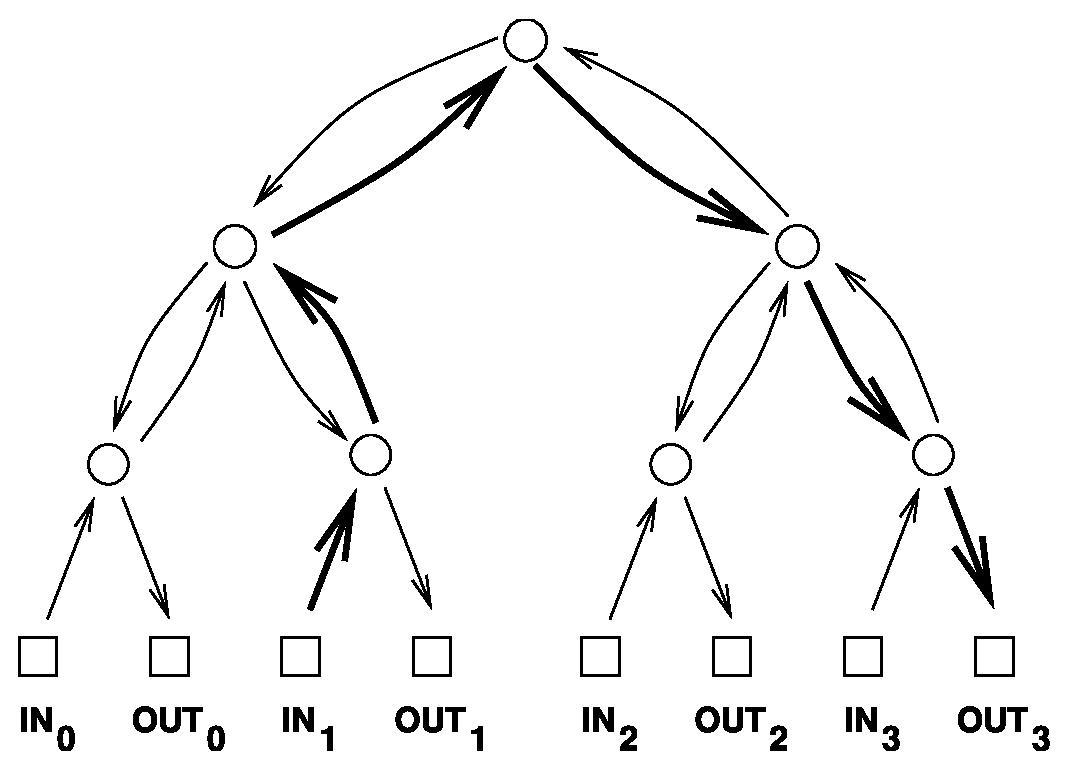
\includegraphics[width = 4in]{bintree-notes}
\end{figure}
The kinds of communication networks we consider aim to transmit packets of
data between computers, processors, telephones, or other devices.  The
term \term{packet} refers to some roughly fixed-size quantity of data---
256 bytes or 4096 bytes or whatever.  In this diagram and many that
follow, the squares represent \term{terminals}, sources and destinations
for packets of data.  The circles represent \term{switches}, which direct
packets through the network.  A switch receives packets on incoming edges
and relays them forward along the outgoing edges.  Thus, you can imagine a
data packet hopping through the network from an input terminal, through a
sequence of switches joined by directed edges, to an output terminal.

Recall that there is a unique simple path between every pair of vertices
in a tree.  So the natural way to route a packet of data from an input
terminal to an output in the complete binary tree is along the
corresponding directed path.  For example, the route of a packet traveling
from input 1 to output 3 is shown in bold.

\section{Routing Problems}

Communication networks are supposed to get packets from inputs to outputs,
with each packet entering the network at its own input switch and arriving
at its own output switch.  We're going to consider several different
communication network designs, where each network has $N$ inputs and
$N$ outputs; for convenience, we'll assume $N$ is a power of two.

Which input is supposed to go where is specified by a permutation of
$\set{0, 1, \dots, N - 1}$.  So a permutation, $\pi$, defines a \term{
  routing problem}: get a packet that starts at input $i$ to output
$\pi(i)$.  A \term{routing}, $P$, that \term{solves} a routing problem,
$\pi$, is a set of paths from each input to its specified output.  That
is, $P$ is a set of $n$ paths, $P_i$, for $i=0\dots,N-1$, where $P_i$ goes
from input $i$ to output $\pi(i)$.

\section{Network Diameter}

The delay between the time that a packets arrives at an input and arrives
at its designated output is a critical issue in communication networks.
Generally this delay is proportional to the length of the path a packet
follows.  Assuming it takes one time unit to travel across a wire,
\begin{staffnotes}
and that there are no additional delays at switches,
\end{staffnotes}
the delay of a packet will be the number of wires it crosses going from
input to output.

\begin{staffnotes}

\footnote{Latency is often measured as the number of switches that
a packet must pass through when traveling between the most distant input
and output, since switches usually have the biggest impact on network
speed.  For example, in the complete binary tree example, the packet
traveling from input 1 to output 3 crosses 5 switches.}

\end{staffnotes}

Generally packets are routed to go from input to output by the shortest
path possible.  With a shortest path routing, the worst case delay is the
distance between the input and output that are farthest apart.  This is
called the \term{diameter} of the network.  In other words, the diameter
of a network\footnote{The usual definition of \emph{diameter} for a
general \textit{graph} (simple or directed) is the largest distance
between \emph{any} two vertices, but in the context of a communication
network we're only interested in the distance between inputs and outputs,
not between arbitrary pairs of vertices.} is the maximum length of any
shortest path between an input and an output.  For example, in the
complete binary tree above, the distance from input 1 to output 3 is six.
No input and output are farther apart than this, so the diameter of this
tree is also six.

More generally, the diameter of a complete binary tree with $N$ inputs and
outputs is $2 \log N + 2$.  (All logarithms in this lecture--- and in most
of computer science ---are base 2.)  This is quite good, because the
logarithm function grows very slowly.  We could connect up $2^{10} = 1024$
inputs and outputs using a complete binary tree and the worst input-output
delay for any packet would be this diameter, namely, $2 \log(2^{10}) + 2 =
22$.

\subsection{Switch Size}

One way to reduce the diameter of a network is to use larger switches.
For example, in the complete binary tree, most of the switches have
three incoming edges and three outgoing edges, which makes them $3
\times 3$ switches.  If we had $4 \times 4$ switches, then we could
construct a complete \textit{ternary} tree with an even smaller
diameter.  In principle, we could even connect up all the inputs and
outputs via a single monster $N \times N$ switch.

\begin{staffnotes}
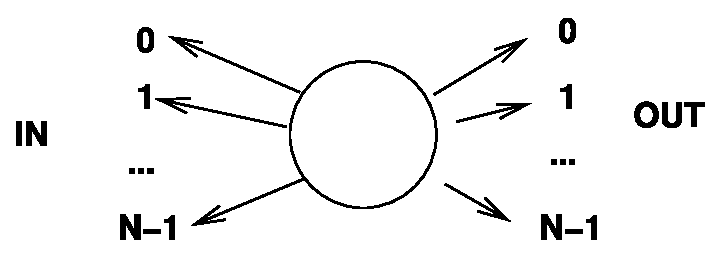
\includegraphics[width = 4in]{monster-switch}
\end{staffnotes}

This isn't very productive, however, since we've just concealed the
original network design problem inside this abstract switch.
Eventually, we'll have to design the internals of the monster switch
using simpler components, and then we're right back where we started.
So the challenge in designing a communication network is figuring out
how to get the functionality of an $N \times N$ switch using
fixed size, elementary devices, like $3 \times 3$ switches.
\begin{solution}
Following this approach, we can build arbitrarily large networks
just by adding in more building blocks. 
\end{solution}

\section{Switch Count}

Another goal in designing a communication network is to use as few
switches as possible.  The number of switches in a complete binary tree is
$1 + 2 + 4 + 8 + \cdots + N$, since there is 1 switch at the top (the
``root switch''), 2 below it, 4 below those, and so forth.  By the
formula~\eqref{geometric-n} for geometric sums, the total number of
switches is $2 N - 1$, which is nearly the best possible with $3 \times 3$
switches.

\section{Network  Latency}

We'll sometimes be choosing routings through a network that optimize some
quantity besides delay.  For example, in the next section we'll be trying
to minimize packet congestion.  When we're not minimizing delay, shortest
routings are not always the best, and in general, the delay of a packet
will depend on how it is routed.  For any routing, the most delayed packet
will be the one that follows the longest path in the routing.  The length
of the longest path in a routing is called its \term{latency}.

%NEEDS REVISION:

The latency of a \emph{network} depends on what's being optimized.  It is
measured by assuming that optimal routings are always chosen in getting
inputs to their specified outputs.  That is, for each routing problem,
$\pi$, we choose an optimal routing that solves $\pi$.  Then \term{network
  latency} is defined to be the largest routing latency among these
optimal routings.  Network latency will equal network diameter if routings
are always chosen to optimize delay, but it may be significantly larger if
routings are chosen to optimize something else.

For the networks we consider below, paths from input to output are
uniquely determined (in the case of the tree) or all paths are the same
length, so network latency will always equal network diameter.


\section{Congestion}

The complete binary tree has a fatal drawback: the root switch is a
bottleneck.  At best, this switch must handle an enormous amount of
traffic: every packet traveling from the left side of the network to the
right or vice-versa.  Passing all these packets through a single switch
could take a long time.  At worst, if this switch fails, the network is
broken into two equal-sized pieces.

For example, if the routing problem is given by the identity permutation,
$\ident{}(i) \eqdef i$, then there is an easy routing, $P$, that solves
the problem: let $P_i$ be the path from input $i$ up through one switch
and back down to output $i$.  On the other hand, if the problem was given
by $\pi(i) \eqdef (N - 1) - i$, then in \emph{any} solution, $Q$, for
$\pi$, each path $Q_i$ beginning at input $i$ must eventually loop all
the way up through the root switch and then travel back down to output $(N
- 1) - i$.  These two situations are illustrated below.
\begin{figure}
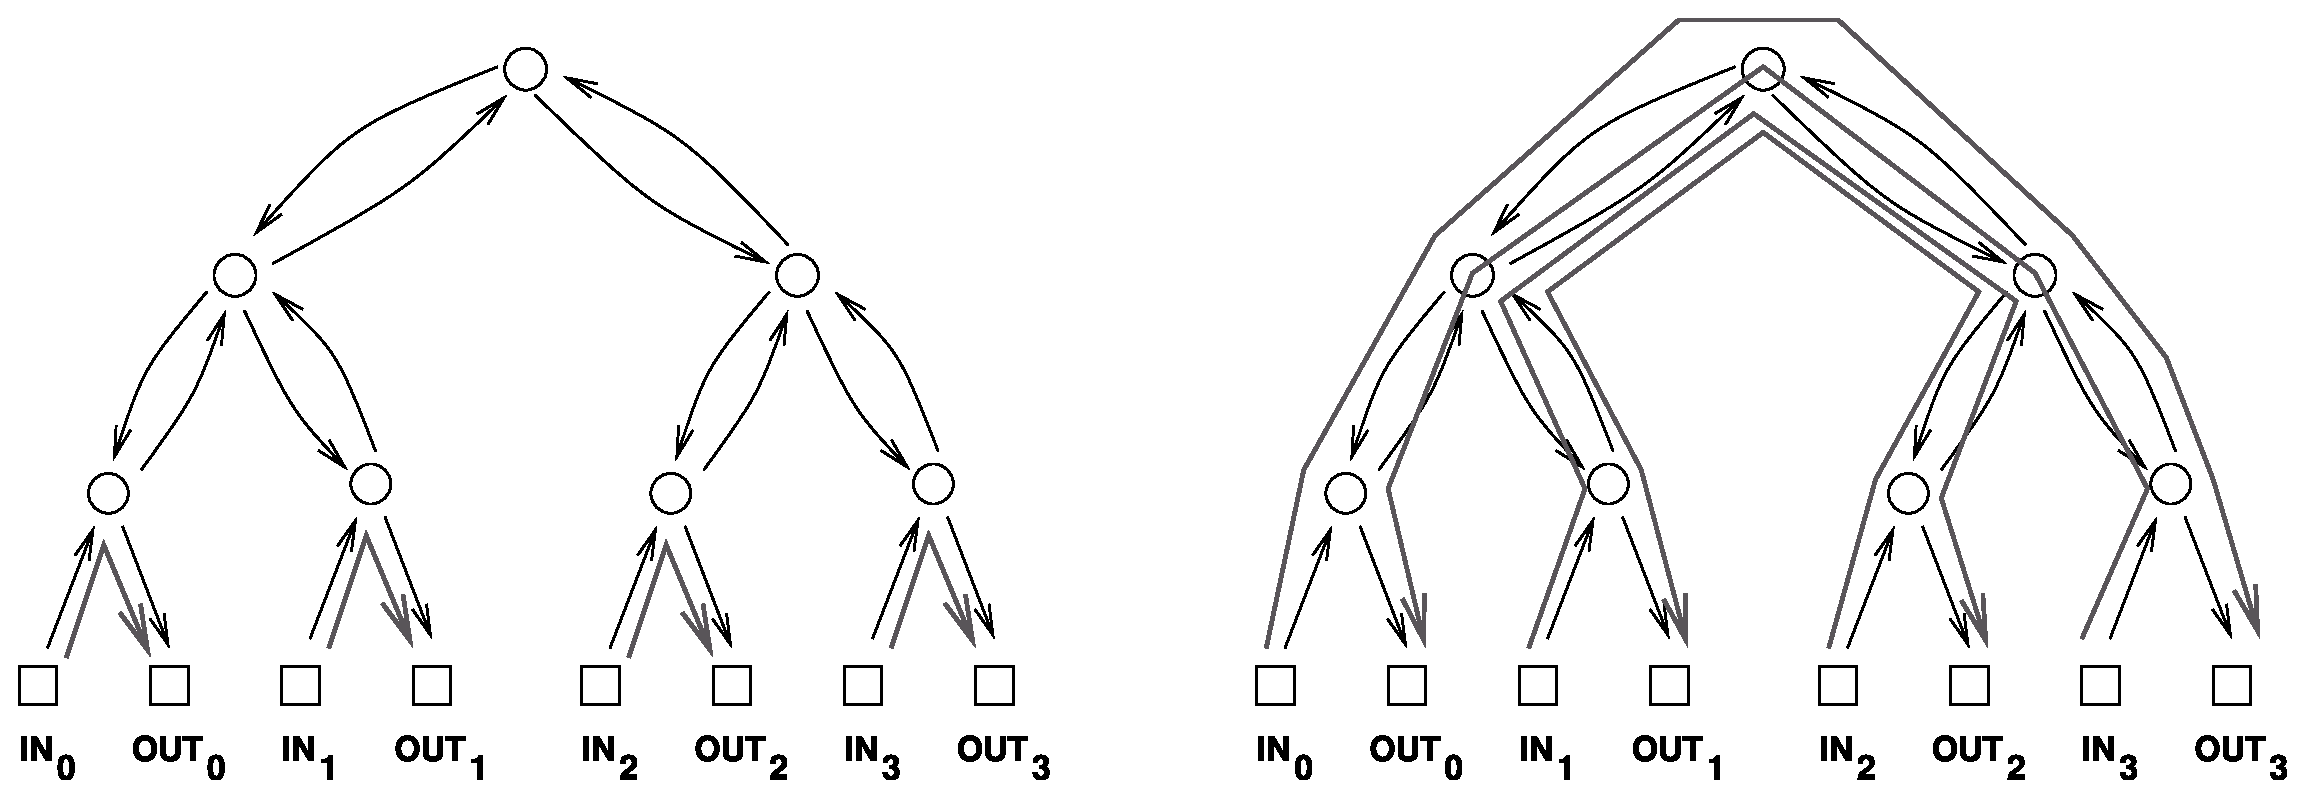
\includegraphics[width = 4in]{bintree2}
\end{figure}
We can distinguish between a ``good'' set of paths and a ``bad'' set based
on congestion.  The \term{congestion} of a routing, $P$, is equal to the
largest number of paths in $P$ that pass through a single switch.  For
example, the congestion of the routing on the left is 1, since at most 1
path passes through each switch.  However, the congestion of the routing
on the right is 4, since 4 paths pass through the root switch (and the two
switches directly below the root).  Generally, lower congestion is better
since packets can be delayed at an overloaded switch.

By extending the notion of congestion to networks, we can also distinguish
between ``good'' and ``bad'' networks with respect to bottleneck problems.
For each routing problem, $\pi$, for the network, we assume a routing is
chosen that optimizes congestion, that is, that has the minimum congestion
among all routings that solve $\pi$.  Then the largest congestion that
will ever be suffered by a switch will be the maximum congestion among
these optimal routings.  This ``maximin'' congestion is called the
\term{congestion of the network}.

\begin{staffnotes}

You may find it helpful to think about max congestion in terms of a value
game.  You design your spiffy, new communication network; this defines the
game.  Your opponent makes the first move in the game: she inspects your
network and specifies a permutation routing problem that will strain your
network.\iffalse
That is, her first move is a specification of which input terminals must
send a packet to which output terminals.
\fi
You move second: given her specification, you choose the precise paths
that the packets should take through your network; you're trying to avoid
overloading any one switch.  Then her next move is to pick a switch with
as large as possible a number of packets passing through it; this number
is her score in the competition.  The max congestion of your network is
the largest score she can ensure; in other words, it is precisely the
max-value of this game.

For example, if your enemy were trying to defeat the complete binary
tree, she would choose a permutation like $\pi(i) = (N - 1) - i$.
Then for \textit{every} packet $i$, you would be forced to select a
path $P_{i, \pi(i)}$ passing through the root switch.  Thus, the max
congestion of the complete binary tree is $N$--- which is horrible!

\end{staffnotes}

So for the complete binary tree, the worst permutation would be $\pi(i)
\eqdef (N - 1) - i$.  Then in every possible solution for $\pi$,
\textit{every} packet, would have to follow a path passing through the
root switch.  Thus, the max congestion of the complete binary tree is $N$
---which is horrible!

Let's tally the results of our analysis so far:
%
\[
\begin{array}{r|c|c|c|c}
\textbf{network} &
\textbf{diameter} &
\textbf{switch size} &
\textbf{\# switches} &
\textbf{congestion} \\ \hline
\text{complete binary tree} & 2 \log N + 2 & 3 \times 3 & 2N - 1 & N \\
\end{array}
\]

\hyperdef{2-D}{array}{\section{2-D Array}}\label{2Darray}

Let's look at an another communication network.  This one is called a
\term{2-dimensional array} or \term{grid}.

\begin{staffnotes}
or \term{crossbar}.
\end{staffnotes}
\begin{figure}
\includegraphics[width = 4in]{grid}
\end{figure}
Here there are four inputs and four outputs, so $N = 4$.

The diameter in this example is 8, which is the number of edges between
input 0 and output 3.  More generally, the diameter of an array with $N$
inputs and outputs is $2N$, which is much worse than the diameter of $2
\log N + 2$ in the complete binary tree.  On the other hand, replacing a
complete binary tree with an array almost eliminates congestion.

\begin{theorem}
The congestion of an $N$-input array is 2.
\end{theorem}

\begin{proof}
First, we show that the congestion is at most 2.  Let $\pi$ be any
permutation.  Define a solution, $P$, for $\pi$ to be the set of paths,
$P_i$, where $P_i$ goes to the right from input $i$ to column $\pi(i)$ and
then goes down to output $\pi(i)$.  Thus, the switch in row $i$ and column
$j$ transmits at most two packets: the packet originating at input
$i$ and the packet destined for output $j$.

Next, we show that the congestion is at least 2.  This follows because in
any routing problem, $\pi$, where $\pi(0) = 0$ and $\pi(N-1) =
N-1$, two packets must pass through the lower left switch.
\end{proof}

As with the tree, the network latency when minimizing congestion is the
same as the diameter.  That's because all the paths between a given input
and output are the same length.

Now we can record the characteristics of the 2-D array.
%
\[
\begin{array}{r|c|c|c|c}
\textbf{network} &
\textbf{diameter} &
\textbf{switch size} &
\textbf{\# switches} &
\textbf{congestion} \\ \hline
\text{complete binary tree} & 2 \log N + 2 & 3 \times 3 & 2N - 1 & N \\
\text{2-D array} & 2 N & 2 \times 2 & N^2 & 2
\end{array}
\]
%
The crucial entry here is the number of switches, which is $N^2$.
This is a major defect of the 2-D array; a network of size $N = 1000$
would require a \textit{million} $2 \times 2$ switches!  Still, for
applications where $N$ is small, the simplicity and low congestion of
the array make it an attractive choice.


\section{Butterfly}

The Holy Grail of switching networks would combine the best properties
of the complete binary tree (low diameter, few switches) and of the
array (low congestion).  The \term{butterfly} is a widely-used
compromise between the two.  \iffalse
Here is a butterfly network with $N = 8$
inputs and outputs.
\begin{figure}
\includegraphics[width = 4in]{butterfly2}
\end{figure}
The structure of the butterfly is certainly more complicated than that
of the complete binary tree or 2-D array!  Let's work through the
various parts of the butterfly.

All the terminals and switches in the network are arranged in $N$
rows.  In particular, input $i$ is at the left end of row $i$, and
output $i$ is at the right end of row $i$.  Now let's label the rows
in $\textit{binary}$; thus, the label on row $i$ is the binary number
$b_1 b_2 \dots b_{\log N}$ that represents the integer $i$.

Between the inputs and the outputs, there are $\log(N) + 1$ levels of
switches, numbered from 0 to $\log N$.  Each level consists of a
column of $N$ switches, one per row.  Thus, each switch in the network
is uniquely identified by a sequence $(b_1, b_2, \dots, b_{\log N},
l)$, where $b_1 b_2 \dots b_{\log N}$ is the switch's row in binary
and $l$ is the switch's level.

All that remains is to describe how the switches are connected up.
The basic connection pattern is expressed below in a compact notation:
%
\[
(b_1, b_2, \dots, b_{l+1}, \dots, b_{\log N}, l)
\begin{array}{l}
\nearrow \\
\searrow
\end{array}
\begin{array}{l}
(b_1, b_2, \dots, b_{l+1}, \dots, b_{\log N}, l + 1) \\
\\
(b_1, b_2, \dots, \overline{b_{l+1}}, \dots, b_{\log N}, l + 1)
\end{array}
\]
%
This says that there are directed edges from switch $(b_1, b_2,
\dots, b_{\log N}, l)$ to two switches in the next level.  One edge
leads to the switch in the \textit{same} row, and the other edge leads
to the switch in the row obtained by \textit{inverting} bit $l + 1$.
For example, referring back to the illustration of the size $N = 8$
butterfly, there is an edge from switch $(0, 0, 0, 0)$ to switch $(0,
0, 0, 1)$, which is in the same row, and to switch $(1, 0, 0, 1)$,
which is the row obtained by inverting bit $l + 1 = 1$.
\fi

A good way to understand butterfly networks is as a recursive data
type.  The recursive definition works better if we define just the
switches and their connections, omitting the terminals.  So we
recursively define $F_n$ to be the switches and connections of the
butterfly net with $N \eqdef 2^n$ input and output switches.

The base case is $F_1$ with 2 input switches and 2 output switches
connected as in Figure~\ref{fig:butterfly-base}.

\begin{figure}
\includegraphics[width = 4in]{butterfly_base}
\caption{$F_1$, the Butterfly Net switches with $N=2^1$.}
\label{fig:butterfly-base}
\end{figure}

\begin{editingnotes}

The butterfly of size $2N$ consists of two butterflies of size $N$, which
are shown in dashed boxes below, and one additional level of switches.
Each switch in the new level has directed edges to a pair of
corresponding switches in the smaller butterflies; one example is
dashed in the figure.

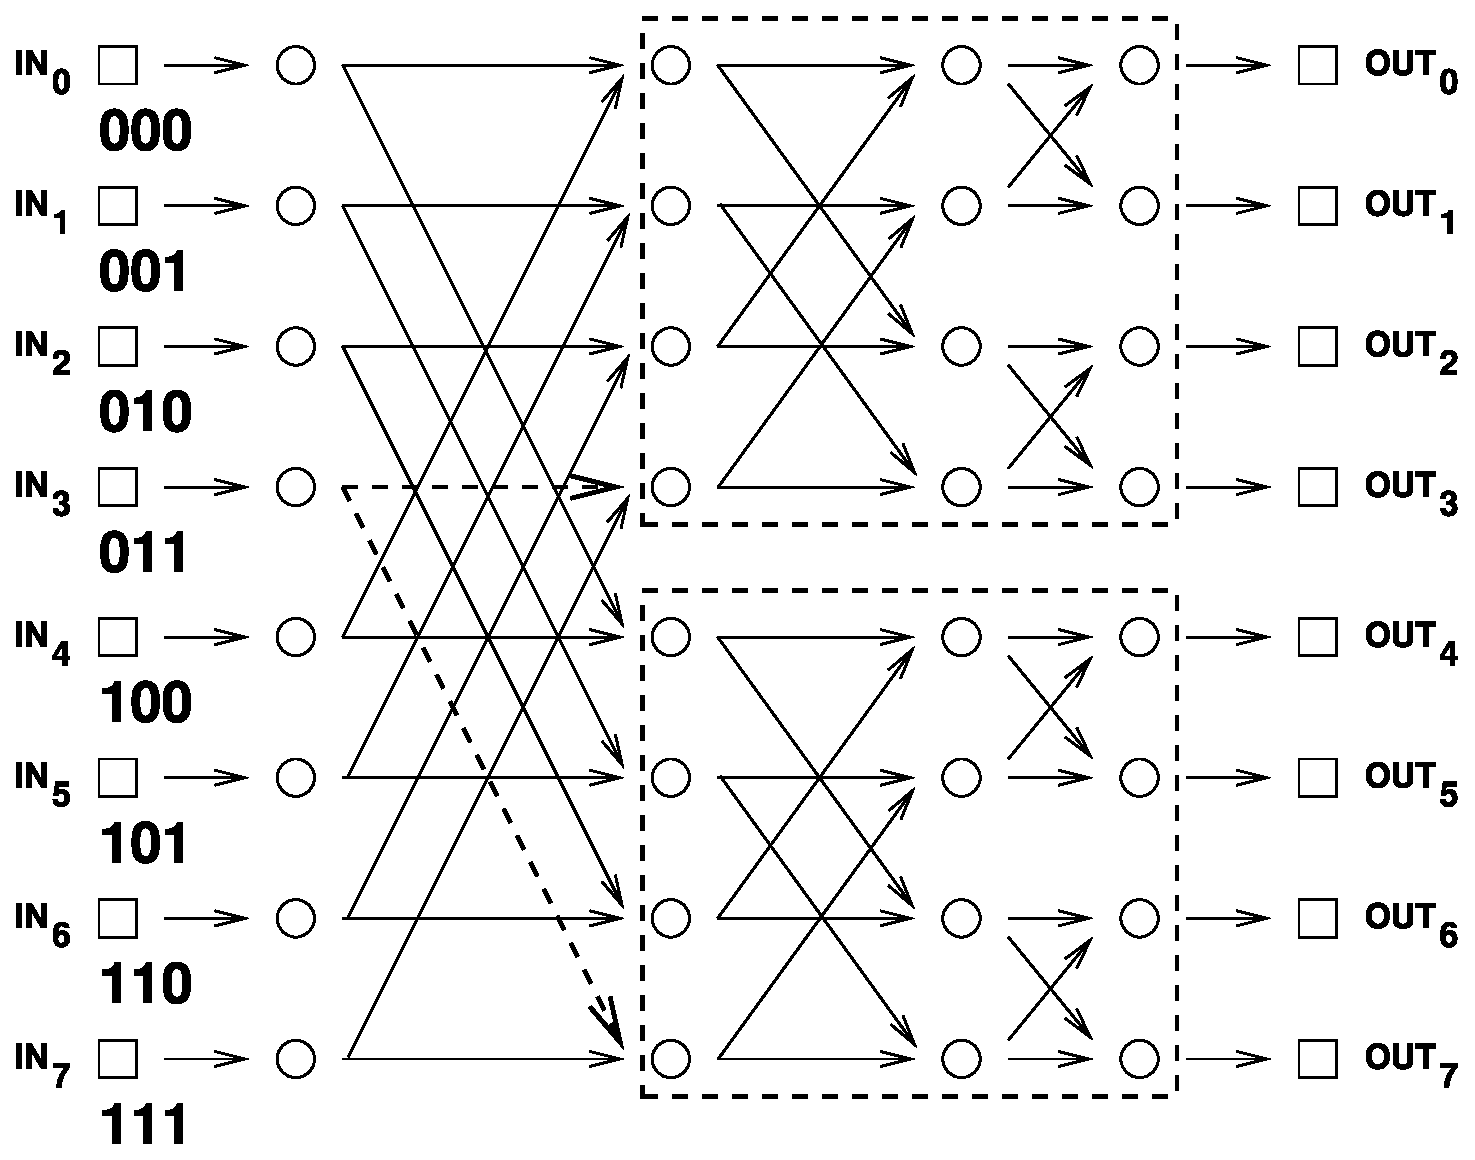
\includegraphics[width = 4in]{butterfly3}

Despite the relatively complicated structure of the butterfly, there
is a simple way to route packets.  In particular, suppose that we want
to send a packet from input $x_1 x_2 \dots x_{\log N}$ to output $y_1
y_2 \dots y_{\log N}$.  (Here we are specifying the input and output
numbers in binary.)  Roughly, the plan is to ``correct'' the first bit
by level 1, correct the second bit by level 2, and so forth.  Thus,
the sequence of switches visited by the packet is:
%
\begin{align*}
(x_1, x_2, x_3, \dots, x_{\log N}, 0)
    & \to (y_1, x_2, x_3, \dots, x_{\log N}, 1) \\
    & \to (y_1, y_2, x_3, \dots, x_{\log N}, 2) \\
    & \to (y_1, y_2, y_3, \dots, x_{\log N}, 3) \\
    & \to \qquad \dots \\
    & \to (y_1, y_2, y_3, \dots, y_{\log N}, \log N) \\
\end{align*}
%
In fact, this is the \textit{only} path from the input to the output!
\end{editingnotes}


In the constructor step, we construct $F_{n+1}$ with $2^{n+1}$ inputs and
outputs out of two $F_n$ nets connected to a new set of $2^{n+1}$ input
switches, as shown in as in Figure~\ref{fig:butterfly-recursive}.  That
is, the $i$th and $2^n+i$th new input switches are each connected to the
same two switches, namely, to the $i$th input switches of each of two
$F_n$ components for $i=1,\dots,2^n$.  The output switches of $F_{n+1}$
are simply the output switches of each of the $F_n$ copies.

\begin{figure}
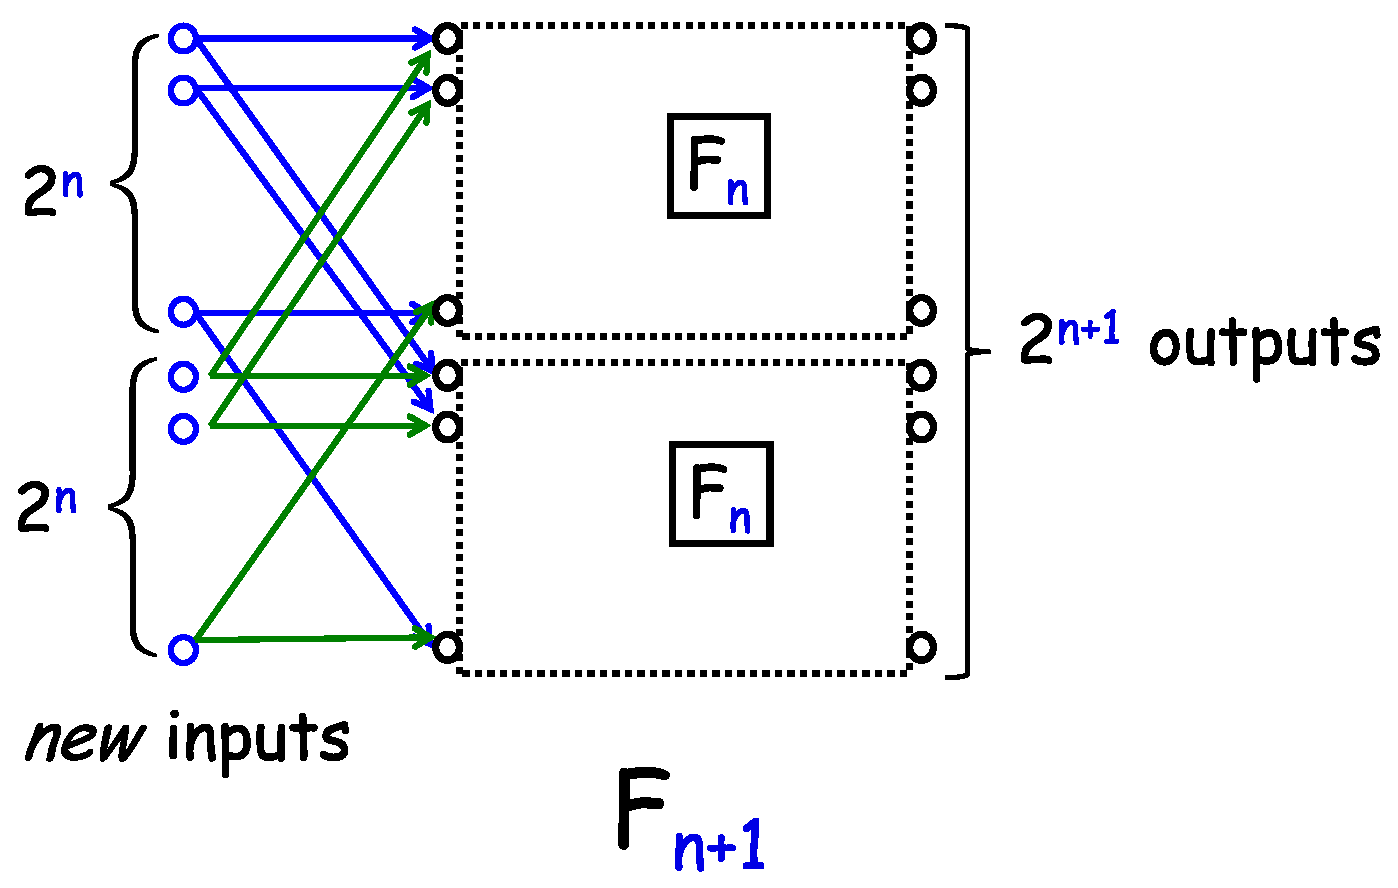
\includegraphics[width = 4in]{butterfly-recursive}
\caption{$F_{n+1}$, the Butterfly Net switches with $2^{n+1}$ inputs
and outputs.}
\label{fig:butterfly-recursive}
\end{figure}

So $F_{n+1}$ is laid out in columns of height $2^{n+1}$ by adding one more
column of switches to the columns in $F_n$.  Since the construction starts
with two columns when $n=1$, the $F_{n+1}$ switches are arrayed in $n+1$
columns.  The total number of switches is the height of the columns times
the number of columns, namely, $2^{n+1}(n+1)$.  Remembering that $n=\log
N$, we conclude that the Butterfly Net with $N$ inputs has $N(\log N +1)$
switches.

Since every path in $F_{n+1}$ from an input switch to an output is the
same length, namely, $n+1$, the diameter of the Butterfly net with
$2^{n+1}$ inputs is this length plus two because of the two edges
connecting to the terminals (square boxes) ---one edge from input
terminal to input switch (circle) and one from output switch to output
terminal.

There is an easy recursive procedure to route a packet through the
Butterfly Net.  In the base case, there is obviously only one way to route
a packet from one of the two inputs to one of the two outputs.  Now
suppose we want to route a packet from an input switch to an output switch
in $F_{n+1}$.  If the output switch is in the ``top'' copy of $F_n$, then
the first step in the route must be from the input switch to the unique
switch it is connected to in the top copy; the rest of the route is
determined by recursively routing the rest of the way in the top copy of
$F_n$.  Likewise, if the output switch is in the ``bottom'' copy of $F_n$,
then the first step in the route must be to the switch in the bottom copy,
and the rest of the route is determined by recursively routing in the
bottom copy of $F_n$.  In fact, this argument shows that the routing is
\emph{unique}: there is exactly one path in the Butterfly Net from each
input to each output, which implies that the network latency when
minimizing congestion is the same as the diameter.

The congestion of the butterfly network is about $\sqrt{N}$, more
precisely, the congestion is $\sqrt{N}$ if $N$ is an even power of 2 and
$\sqrt{N/2}$ if $N$ is an odd power of 2.  A simple proof of this appears
in Problem\ref{PS_butterfly_congestion}.

Let's add the butterfly data to our comparison table:
%
\[
\begin{array}{r|c|c|c|c}
\textbf{network} &
\textbf{diameter} &
\textbf{switch size} &
\textbf{\# switches} &
\textbf{congestion} \\ \hline
\text{complete binary tree} & 2 \log N + 2 & 3 \times 3 & 2N - 1 & N \\
\text{2-D array} & 2 N & 2 \times 2 & N^2 & 2 \\
\text{butterfly} & \log N + 2 & 2 \times 2 & N (\log(N) + 1) & \sqrt{N} \text{ or } \sqrt{N/2}
\end{array}
\]
%
The butterfly has lower congestion than the complete binary tree.  And
it uses fewer switches and has lower diameter than the array.
However, the butterfly does not capture the best qualities of each
network, but rather is a compromise somewhere between the two.  So our
quest for the Holy Grail of routing networks goes on.

\section{Bene\u{s} Network}

In the 1960's, a researcher at Bell Labs named Bene\u{s} had a
remarkable idea.  He obtained a marvelous communication network with
congestion 1 by placing \textit{two} butterflies back-to-back.  This
amounts to recursively growing \term{Bene\u{s} nets} by adding both inputs
and outputs at each stage.  Now we recursively define $B_n$ to be the
switches and connections (without the terminals) of the Bene\u{s} net
with $N \eqdef 2^n$ input and output switches.

The base case, $B_1$, with 2 input switches and 2 output switches is
exactly the same as $F_1$ in Figure~\ref{fig:butterfly-base}.

In the constructor step, we construct $B_{n+1}$ out of two $B_n$ nets
connected to a new set of $2^{n+1}$ input switches \emph{and also} a
new set of $2^{n+1}$ output switches.  This is illustrated in
Figure~\ref{fig:benes-recursive}.

Namely, the $i$th and $2^n+i$th new input switches are each connected to
the same two switches, namely, to the $i$th input switches of each of two
$B_n$ components for $i=1,\dots,2^n$, exactly as in the Butterfly net.  In
addition, the $i$th and $2^n+i$th new \emph{output} switches are connected
to the same two switches, namely, to the $i$th output switches of each of
two $B_n$ components.

\begin{figure}
\includegraphics[width = 4in]{benes_recursive}
%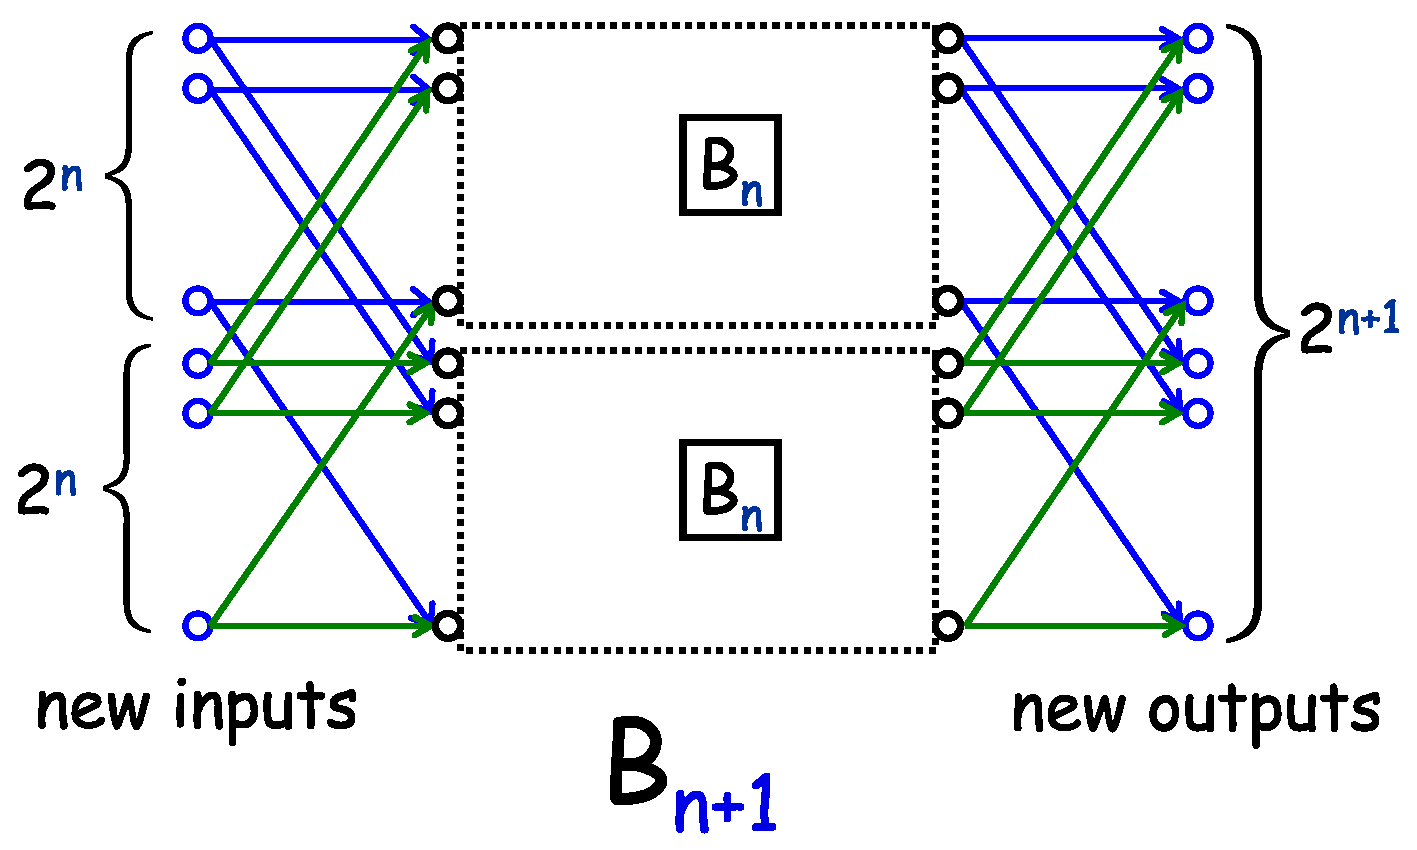
\includegraphics{figures/benes-recursive}
\caption{$B_{n+1}$, the Bene\u{s} Net switches with $2^{n+1}$ inputs
and outputs.}
\label{fig:benes-recursive}
\end{figure}

Now $B_{n+1}$ is laid out in columns of height $2^{n+1}$ by adding two
more columns of switches to the columns in $B_n$.  So the $B_{n+1}$
switches are arrayed in $2(n+1)$ columns.  The total number of
switches is the number of columns times the height of the columns,
namely, $2(n+1)2^{n+1}$.

All paths in $B_{n+1}$ from an input switch to an output are the same
length, namely, $2(n+1)-1$, and the diameter of the Bene\u{s} net with
$2^{n+1}$ inputs is this length plus two because of the two edges
connecting to the terminals.

\begin{staffnotes}

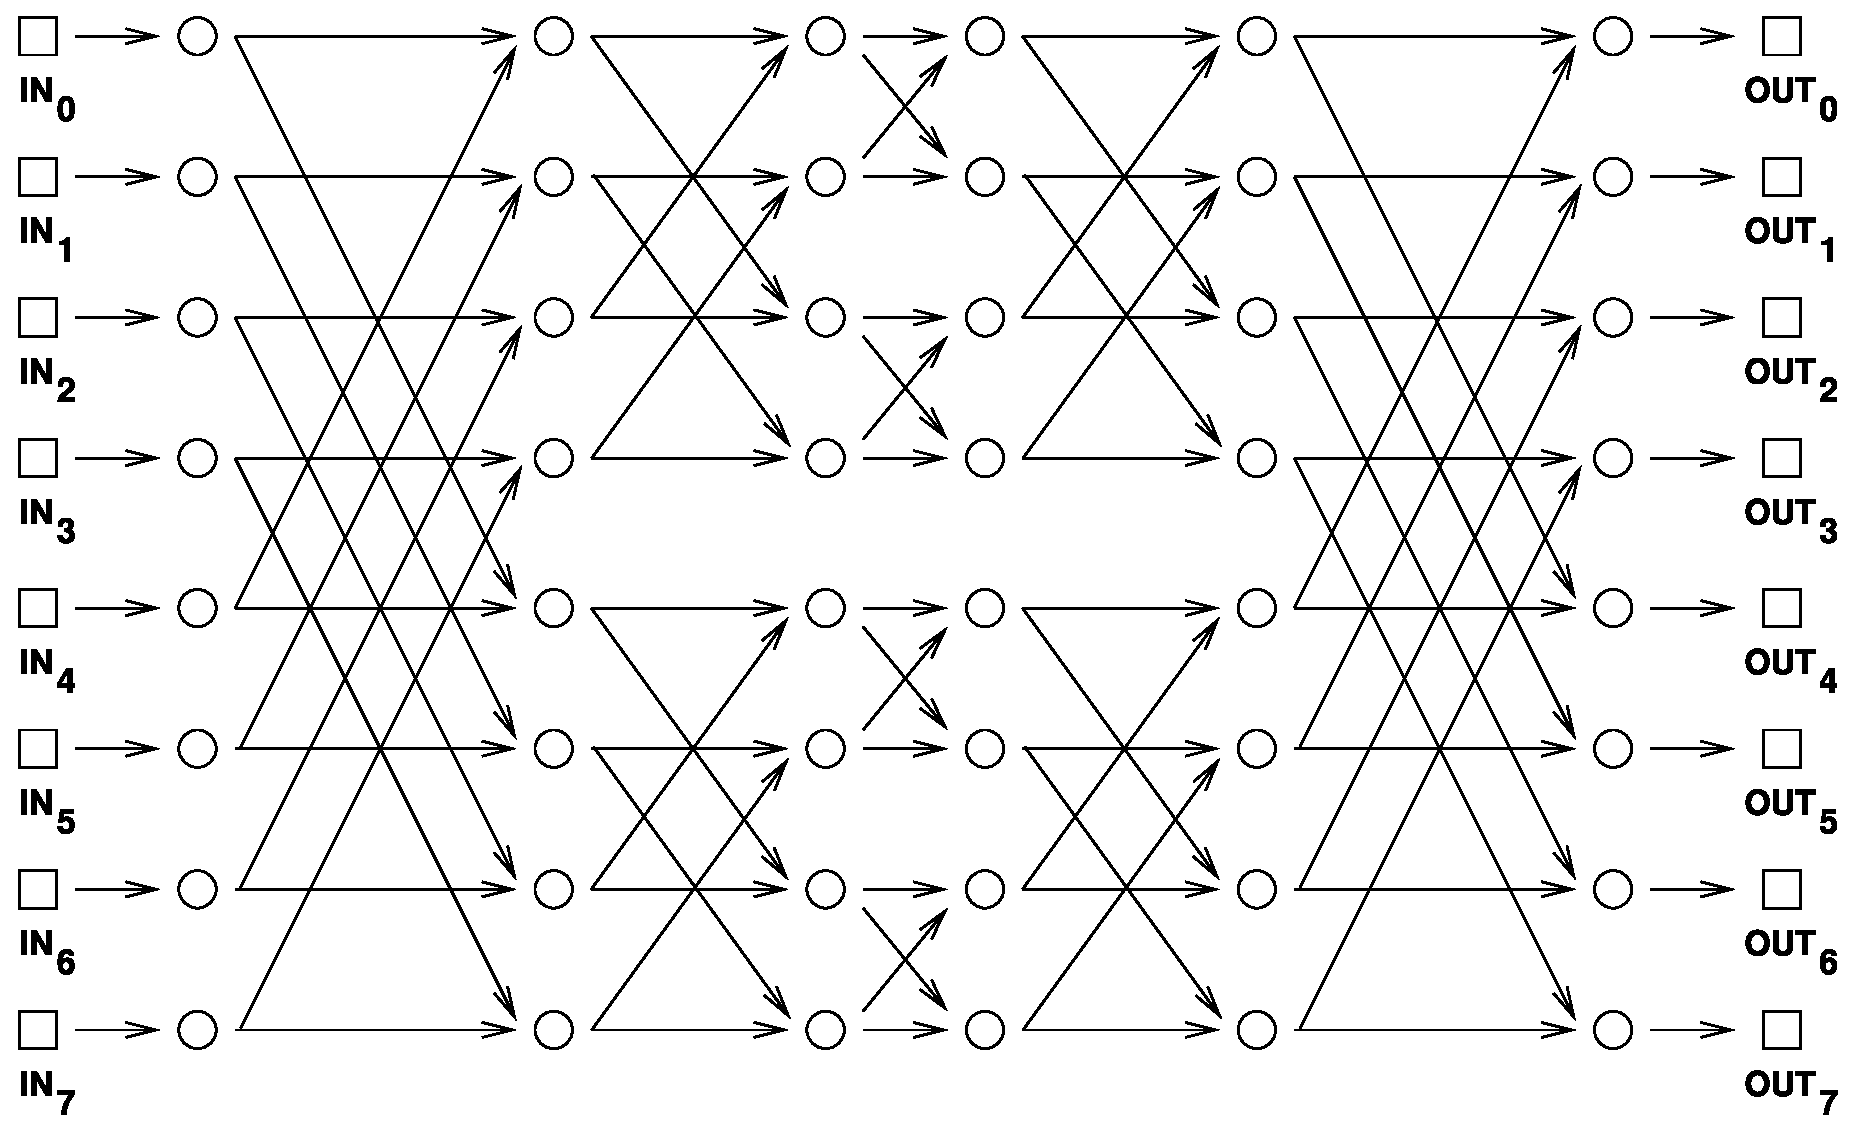
\includegraphics[width = 4in]{benes}

% This should make the construction of the 2-colorable graph in the
% congestion proof just a little more apparent.

This network now has levels labeled $0,\dots ,2 \log N + 1$. For $1 \leq k
\leq \log N$, the connections from level $k-1$ to level $k$ are just as in
the Butterfly network, the connections based on bit $k$. The conections
from level $2 \log N - k + 1$ to level $2 \log N - k + 2$ are also the
ones based on bit $k$.  (Informally, to make the connections from level
$0$ to level $2 \log N +1$ one level at a time, use the connections based
on bits $1,2,3,\dots, \log N - 1, \log N, \log N - 1, \log N - 2, \dots,
3,2,1$ in that order.)

\end{staffnotes}

So Bene\u{s} has doubled the number of switches and the diameter, of
course, but completely eliminates congestion problems!  The proof of
this fact relies on a clever induction argument that we'll come to in
a moment.  Let's first see how the Bene\u{s} network stacks up:
%
\[
\begin{array}{r|c|c|c|c}
\textbf{network} &
\textbf{diameter} &
\textbf{switch size} &
\textbf{\# switches} &
\textbf{congestion} \\ \hline
\text{complete binary tree} & 2 \log N + 2 & 3 \times 3 & 2N - 1 & N \\
\text{2-D array} & 2 N & 2 \times 2 & N^2 & 2 \\
\text{butterfly} & \log N + 2 & 2 \times 2 & N (\log(N) + 1) & \sqrt{N} \text{ or } \sqrt{N/2} \\
\text{Bene\u{s}} & 2 \log N + 1 & 2 \times 2 &  2 N \log N & 1
\end{array}
\]
%
The Bene\u{s} network has small size and diameter, and completely
eliminates congestion.  The Holy Grail of routing networks is in hand!

\begin{theorem}
The congestion of the $N$-input Bene\u{s} network is 1.

\iffalse , where $N = 2^a$ for some $a \geq 1$\fi

\end{theorem}

\begin{proof}
By induction on $n$ where $N=2^n$.  So the induction hypothesis is

\[
P(n) \eqdef  \text{the congestion of $B_n$ is 1}.
\]

\textbf{Base case} ($n=1$): $B_1 =F_1$ and the unique routings in $F_1$
have congestion 1.

\textbf{Inductive step}: We assume that the congestion of an $N=2^n$-input
Bene\u{s} network is 1 and prove that the congestion of a $2N$-input
Bene\u{s} network is also 1.

\textbf{Digression. }  Time out!  Let's work through an example,
develop some intuition, and then complete the proof.  In the Bene\u{s}
network shown below with $N=8$ inputs and outputs, the two
4-input/output subnetworks are in dashed boxes.

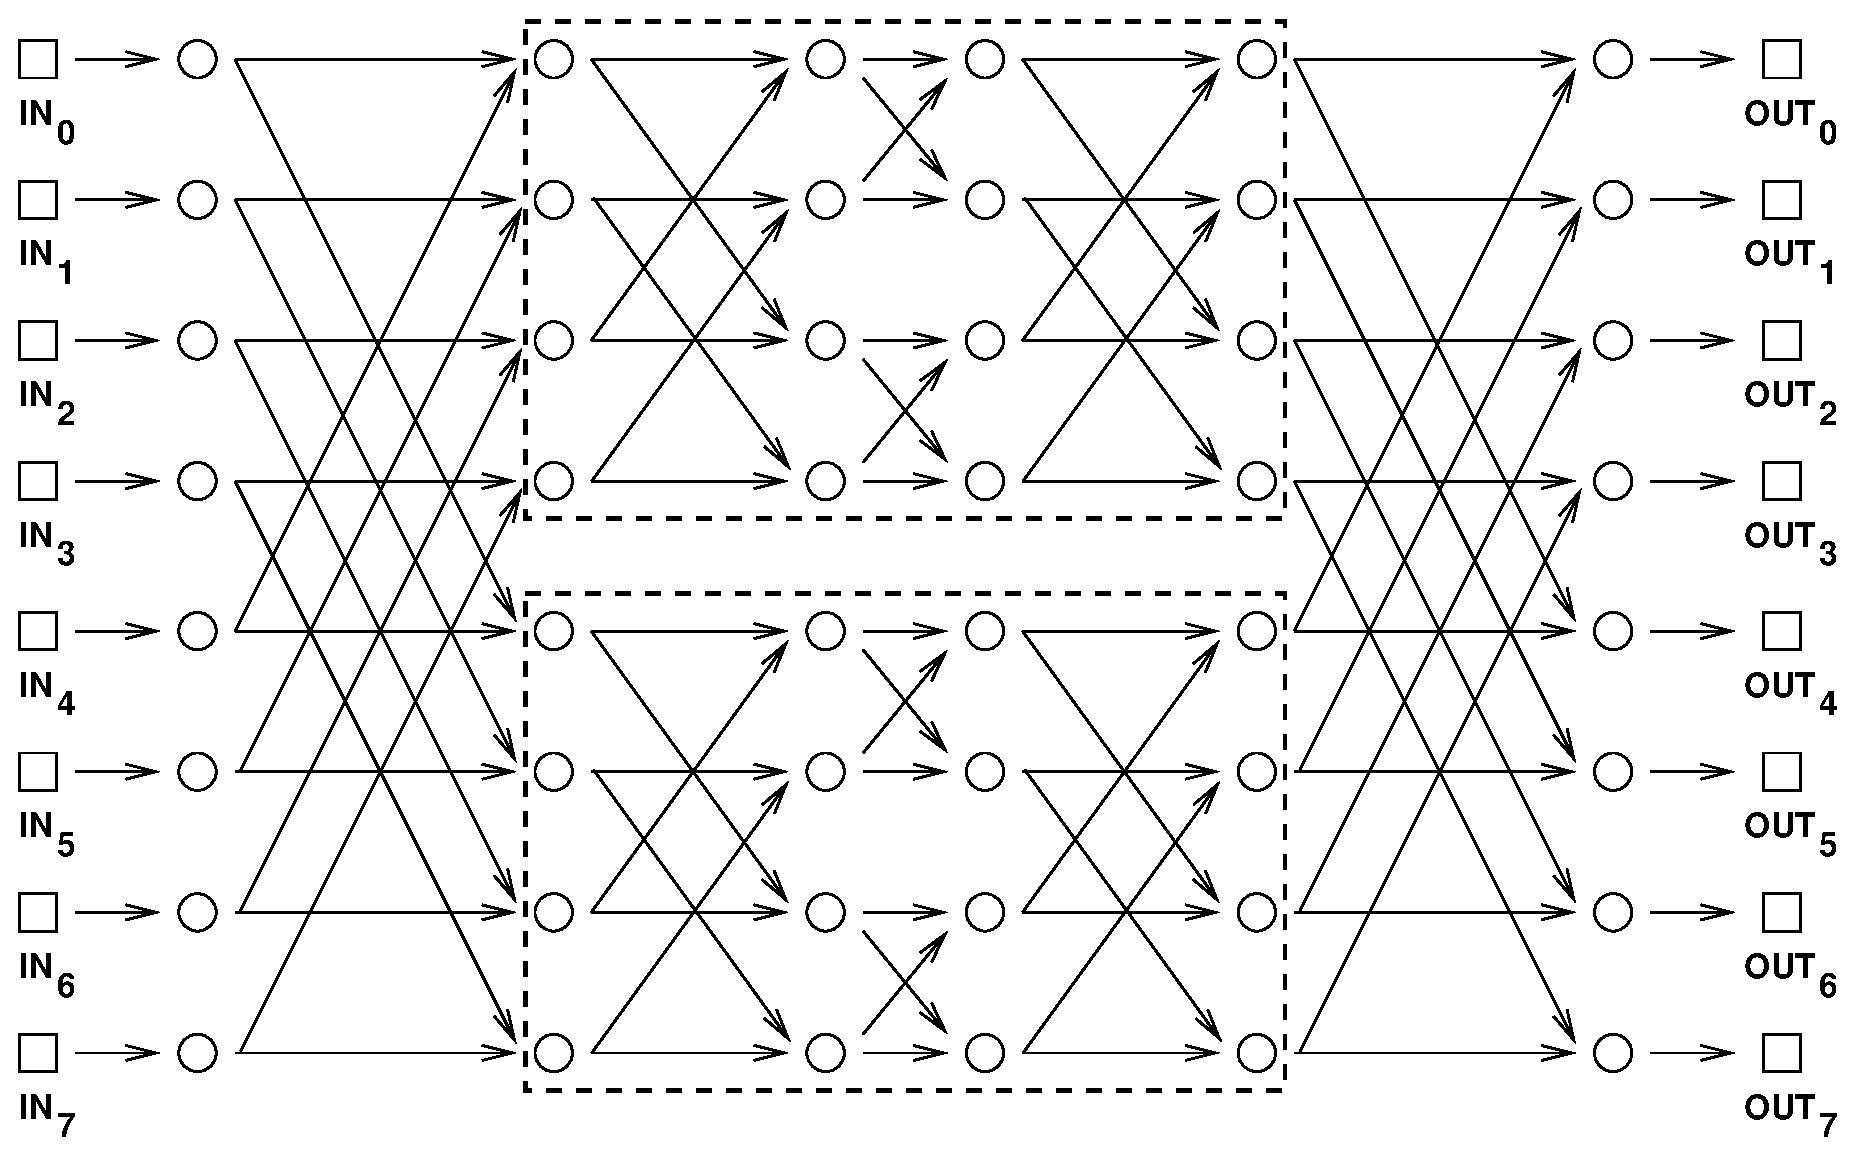
\includegraphics[width = 4in]{benes-decomp}

By the inductive assumption, the subnetworks can each route an
arbitrary permutation with congestion 1.  So if we can guide packets
safely through just the first and last levels, then we can rely on
induction for the rest!  Let's see how this works in an example.
Consider the following permutation routing problem:
%
\begin{align*}
\pi(0) & = 1 & \pi(4) & = 3 \\
\pi(1) & = 5 & \pi(5) & = 6 \\
\pi(2) & = 4 & \pi(6) & = 0 \\
\pi(3) & = 7 & \pi(7) & = 2
\end{align*}

We can route each packet to its destination through either the upper
subnetwork or the lower subnetwork.  However, the choice for one
packet may constrain the choice for another.  For example, we can not
route both packet 0 \textit{and} packet 4 through the same network
since that would cause two packets to collide at a single switch,
resulting in congestion.  So one packet must go through the upper
network and the other through the lower network.  Similarly, packets 1
and 5, 2 and 6, and 3 and 7 must be routed through different networks.
Let's record these constraints in a graph.  The vertices are the 8
packets.  If two packets must pass through different networks, then
there is an edge between them.  Thus, our constraint graph looks like
this:
\begin{center}
\graphic{benes-const1}
\end{center}

Notice that at most one edge is incident to each vertex.

The output side of the network imposes some further constraints.  For
example, the packet destined for output 0 (which is packet 6) and the
packet destined for output 4 (which is packet 2) can not both pass
through the same network; that would require both packets to arrive
from the same switch.  Similarly, the packets destined for outputs 1
and 5, 2 and 6, and 3 and 7 must also pass through different switches.
We can record these additional constraints in our graph with gray
edges:
\begin{center}
\graphic{benes-const2}
\end{center}

Notice that at most one new edge is incident to each vertex.
The two lines drawn between vertices 2 and 6 reflect the two different
reasons why these packets must be routed through different networks.
However, we intend this to be a simple graph; the two lines still
signify a single edge.

Now here's the key insight: suppose that we could color each vertex
either red or blue so that adjacent vertices are colored differently.
Then all constraints are satisfied if we send the red packets through
the upper network and the blue packets through the lower network.
Such a \textit{2-coloring of the graph corresponds to a solution to
  the routing problem}.  The only remaining question is whether the
constraint graph is 2-colorable, which is easy to verify:

\begin{lemma}\label{deg1-union}
  Prove that if the edges of a graph can be grouped into two sets such
  that every vertex has at most 1 edge from each set incident to it, then
  the graph is 2-colorable.
\end{lemma}

\begin{proof}
It is not hard to show that A graph is 2-colorable iff every cycle in
it has even length (see Problem~\ref{PS_no_odd_length_cycles}).  We'll
take this for granted here.

  \iffalse We know from Theorem~\ref{odd-cycle} that \fi
So all we have to do is show that every cycle has even length.  Since
the two sets of edges may overlap, let's call an edge that is in both
sets a \emph{doubled edge}.

There are two cases:

  \textbf{Case 1}: [The cycle contains a doubled edge.]  No other edge can
  be incident to either of the endpoints of a doubled edge, since that
  endpoint would then be incident to two edges from the same set.  So a
  cycle traversing a doubled edge has nowhere to go but back and forth
  along the edge an even number of times.

  \textbf{Case 2}: [No edge on the cycle is doubled.]  Since each vertex
  is incident to at most one edge from each set, any path with no doubled
  edges must traverse successive edges that alternate from one set to the
  other.  In particular, a cycle must traverse a path of alternating edges
  that begins and ends with edges from different sets.  This means the
  cycle has to be of even length.
\end{proof}

For example, here is a 2-coloring of the constraint graph:

\begin{center}
\graphic{benes-const3}
\end{center}

The solution to this graph-coloring problem provides a start
on the packet routing problem:

We can complete the routing in the two smaller Bene\u{s} networks by
induction!  Back to the proof.  \textbf{End of Digression.}

Let $\pi$ be an arbitrary permutation of $\set{0, 1, \dots, N-1}$.  Let $G$
be the graph whose vertices are packet numbers $0, 1, \dots, N-1$ and whose edges
come from the union of these two sets:
\begin{align*}
E_1 \eqdef &  \set{\edge{u}{v} \suchthat \abs{u - v} = N/2},\ \text{and} \\
E_2 \eqdef &  \set{\edge{u}{w} \suchthat \abs{\pi(u) - \pi(w)} = N/2}.
\end{align*}
Now any vertex, $u$, is incident to at most two edges: a unique edge
$\edge{u}{v} \in E_1$ and a unique edge $\edge{u}{w} \in E_2$.  So
according to Lemma~\ref{deg1-union}, there is a 2-coloring for the
vertices of $G$.  Now route packets of one color through the upper
subnetwork and packets of the other color through the lower subnetwork.
Since for each edge in $E_1$, one vertex goes to the upper subnetwork and
the other to the lower subnetwork, there will not be any conflicts in the
first level.  Since for each edge in $E_2$, one vertex comes from the
upper subnetwork and the other from the lower subnetwork, there will not
be any conflicts in the last level.  We can complete the routing within
each subnetwork by the induction hypothesis $P(n)$.
\end{proof}

\begin{problems}
\examproblems
\pinput{MQ_basic_network_problem}

\classproblems
\pinput{CP_Benes_network}
\pinput{CP_binary-tree_network}
\pinput{CP_2_layer_array_network}
\pinput{CP_n-path_network}
\pinput{CP_Megumi_net}

\homeworkproblems
\pinput{PS_Reasoner_net}
\pinput{PS_butterfly_congestion}
\pinput{PS_no_odd_length_cycles}
\end{problems}

\iffalse
In class, you will work through an example in which you route packets
using this recursive idea!
\fi

\endinput

   %recursive; uses digraphs, simple graph coloring

\part{Counting}

\documentclass[12pt,twoside]{article}
\usepackage{fancyhdr}
\usepackage{light}
\usepackage{float}
\usepackage{subfigure}
\usepackage{enumitem}
\usepackage{graphicx}
\RequirePackage{cases}


%\showsolutions
\hidesolutions

\begin{document}

\begin{problem}{20}
\textbf{Asymptotic notation} 
%// From 6.006 Spring 2008 quiz 1 and Fall 2014 quiz 1

For each function $f(n)$ along the left side of the table,
and for each function $g(n)$ across the top, write $O$,
$\Omega$, or $\Theta$ in the appropriate space, depending on whether
$f(n)=O(g(n))$, $f(n)=\Omega(g(n))$, or $f(n)=\Theta(g(n))$.
If more than one such relation holds between $f(n)$ and $g(n)$,
write only the strongest one. The first row is a demo solution for $f(n)=n^2$.

\ifshowsolutions 
\begin{center}
\begin{tabular}{|c|c||c|c|c|c|}
\cline{3-6}
\multicolumn{2}{c||}{} & \multicolumn{4}{c|}{} \\
\multicolumn{2}{c||}{} & \multicolumn{4}{c|}{$g(n)$} \\
\multicolumn{2}{c||}{} & \multicolumn{4}{c|}{} \\
\cline{3-6}
\multicolumn{2}{c||}{}
                   & \hspace*{1in} & \hspace*{1in} & \hspace*{1in} & \hspace*{1in}\\
\multicolumn{2}{c||}{}
                   &       $n\log{n}$       &  $\log(n^{0.1})$     &      $\log(\log(n!))$   &   $2^{\sqrt{n}}$ \\
\multicolumn{2}{c||}{}
                   &                 &                 &             &  \\
\hline
\hline
\hspace*{0.5in}
&                    & \hspace*{1in} & \hspace*{1in} & \hspace*{1in} &\\
& $n$               & $O$    & $\Omega$    & $\Omega$ & $O$   \\
&                    &               &                 &             &   \\
\cline{2-6}
&                    & \hspace*{1in} & \hspace*{1in} & \hspace*{1in}&\\
& $n^{1.1}$           &      $\Omega$      &       $\Omega$            &      $\Omega$    &   $O$    \\
&                    &                 &                 &             &   \\
\cline{2-6}
&                    & \hspace*{1in} & \hspace*{1in} & \hspace*{1in} &\\
& $\sqrt{2^n}$         &      $\Omega$         &       $\Omega$         &    $\Omega$     &  $\Omega$         \\
$f(n)$
&                    &                 &                 &             &  \\
\cline{2-6}
&                    & \hspace*{1in} & \hspace*{1in} & \hspace*{1in} &\\
& $n\log_{30}{n}$    &     $\Theta$            &     $\Omega$              &    $\Omega$     &   $O$     \\
&                    &                 &                 &             &  \\
\cline{2-6}
&                    & \hspace*{1in} & \hspace*{1in} & \hspace*{1in} &\\
& $\log(n/\log n)$  &      $O$           &    $\Theta$             &  $\Theta$   &  $O$        \\
&                    &                 &                 &              &  \\
\cline{2-6}
&                    & \hspace*{1in} & \hspace*{1in} & \hspace*{1in} &\\
& $\binom{2n}{n}$  &      $\Omega$             &         $\Omega$          &    $\Omega$   &    $\Omega$    \\
&                    &                 &                 &              & \\
%\cline{2-7}
%&                    & \hspace*{1in} & \hspace*{1in} & \hspace*{1in}& \hspace*{1in}&\\
%& $1$               &                 &                 &             & &  \\
%&                    &                 &                 &             &  & \\
\hline
\end{tabular}
\end{center}

\else
\begin{center}
\begin{tabular}{|c|c||c|c|c|c|}
\cline{3-6}
\multicolumn{2}{c||}{} & \multicolumn{4}{c|}{} \\
\multicolumn{2}{c||}{} & \multicolumn{4}{c|}{$g(n)$} \\
\multicolumn{2}{c||}{} & \multicolumn{4}{c|}{} \\
\cline{3-6}
\multicolumn{2}{c||}{}
                   & \hspace*{1.0in} & \hspace*{1.0in} & \hspace*{1.0in} & \hspace*{1.0in}\\
\multicolumn{2}{c||}{}
                   &       $n$       &  $n \log_2 n$     &      $n^2$   &   $2^{\sqrt{n}}$ \\
\multicolumn{2}{c||}{}
                   &                 &                 &             &    \\
\hline
\hline
\hspace*{0.5in}
&                    & \hspace*{1.0in} & \hspace*{1.0in} & \hspace*{1.0in} & \\
& $n^2$               & \large $\Omega$   & \large $\Omega$   & \large $\Theta$ & $O$ \\
&                    &                 &                 &             &   \\
\cline{2-6}
&                    & \hspace*{1.0in} & \hspace*{1.0in} & \hspace*{1.0in}&\\
& $n^{1.5}$           &                 &                 &        &        \\
&                    &                 &                 &             &   \\
\cline{2-6}
&                    & \hspace*{1.0in} & \hspace*{1.0in} & \hspace*{1.0in} &\\
& $\sqrt{2^n}$         &                 &                 &       &         \\
$f(n)$
&                    &                 &                 &             &   \\
\cline{2-6}
&                    & \hspace*{1.0in} & \hspace*{1.0in} & \hspace*{1.0in} &\\
& $n\sqrt{\log_2 n}$    &                 &                 &       &         \\
&                    &                 &                 &             &   \\
\cline{2-6}
&                    & \hspace*{1.0in} & \hspace*{1.0in} & \hspace*{1.0in} &\\
& $n \log_{30} n$  &                 &                 &              &  \\
&                    &                 &                 &              &  \\
\cline{2-6}
&                    & \hspace*{1.0in} & \hspace*{1.0in} & \hspace*{1.0in}&\\
& $n!$               &                 &                 &             &   \\
&                    &                 &                 &             &   \\
\hline
\end{tabular}
\end{center}
\fi


\end{problem}

\end{document}
 %%

\chapter{Cardinality Rules}\label{counting_chap}

\newcommand{\Jay}{Bob}
\newcommand{\Jer}{Ted}

\section{Counting One Thing by Counting Another}\label{bijection_counting_sec}

How do you count the number of people in a crowded room?  You could
count heads, since for each person there is exactly one head.
Alternatively, you could count ears and divide by two.  Of course, you
might have to adjust the calculation if someone lost an ear in a
pirate raid or someone was born with three ears.  The point here is
that you can often \emph{count one thing by counting another}, though
some fudge factors may be required.  This is a central theme of
counting, from the easiest problems to the hardest.  In fact, we've
already seen this technique used in Theorem~\ref{powset_fincard} where
the number of subsets of an $n$-element set was proved to be the same as
the number of length-$n$ bit-strings by describing a bijection
between the subsets and the bit-strings.

The most direct way to count one thing by counting another is to find
a bijection between them, since if there is a bijection between two
sets, then the sets have the same size.  This important fact is
commonly known as the \term{Bijection Rule}.  We've already seen it as
the \idx{Mapping Rules} bijective case~\eqref{bij_same_fincard}.

\subsection{The Bijection Rule}\label{sec:donut_bij}

\iffalse
\begin{rul}[Bijection Rule]\label{rul:bijection}
If there is a bijection $f: A \to B$ between $A$ and~$B$, then
$\card{A} = \card{B}$.
\end{rul}
\fi

The Bijection Rule acts as a magnifier of counting ability; if you
figure out the size of one set, then you can immediately determine the
sizes of many other sets via bijections.  For example, let's look at
the two sets mentioned at the beginning of Part~\ref{part:counting}:
%
\begin{align*}
A & = \text{all ways to select a dozen donuts when five varieties are available} \\
B & = \text{all 16-bit sequences with exactly 4 ones}
\end{align*}

An example of an element of set $A$ is:
%
\[
\underbrace{0\ 0}_{\text{chocolate}} \quad
\underbrace{}_{\text{lemon-filled}} \quad
\underbrace{0\ 0\ 0\ 0\ 0\ 0}_{\text{sugar}} \quad
\underbrace{0\ 0}_{\text{glazed}} \quad
\underbrace{0\ 0}_{\text{plain}}
\]
Here, we've depicted each donut with a $0$ and left a gap between
the different varieties.  Thus, the selection above contains two
chocolate donuts, no lemon-filled, six sugar, two glazed, and two
plain.  Now let's put a 1 into each of the four gaps:
\[
\underbrace{0\ 0}_{\text{chocolate}} \quad 1 \quad
\underbrace{}_{\text{lemon-filled}} \quad 1 \quad
\underbrace{0\ 0\ 0\ 0\ 0\ 0}_{\text{sugar}} \quad 1 \quad
\underbrace{0\ 0}_{\text{glazed}} \quad 1 \quad
\underbrace{0\ 0}_{\text{plain}}
\]
and close up the gaps:
\[
0011000000100100 \,.
\]
We've just formed a 16-bit number with exactly 4 ones ---an element of
$B$!

This example suggests a bijection from set $A$ to set $B$: map a dozen
donuts consisting of:
%
\[
\text{$c$ chocolate, $l$ lemon-filled, $s$ sugar, $g$ glazed, and $p$ plain}
\]
%
to the sequence:
%
\[
\underbrace{\ 0 \ldots 0\ }_{\text{$c$}} \quad 1 \quad
\underbrace{\ 0 \ldots 0\ }_{\text{$l$}} \quad 1 \quad
\underbrace{\ 0 \ldots 0\ }_{\text{$s$}} \quad 1 \quad
\underbrace{\ 0 \ldots 0\ }_{\text{$g$}} \quad 1 \quad
\underbrace{\ 0 \ldots 0\ }_{\text{$p$}}
\]

The resulting sequence always has 16 bits and exactly 4 ones, and thus
is an element of $B$.  Moreover, the mapping is a bijection: every
such bit sequence comes from exactly one order of a dozen donuts.
Therefore, $\card{A} = \card{B}$ by the Bijection Rule.  More generally,
\begin{lemma}\label{lem:donut_bij}
The number of ways to select $n$ donuts when $k$ flavors are available is
the same as the number of length-$n$ binary sequences with $k-1$ ones.
\end{lemma}

This example demonstrates the power of the bijection rule.
We managed to prove that two very different sets are actually the same
size ---even though we don't know exactly how big either one is.  But
as soon as we figure out the size of one set, we'll immediately know
the size of the other.

This particular bijection might seem frighteningly ingenious if you've
not seen it before.  But you'll use essentially this same argument
over and over, and soon you'll consider it routine.

\section{Counting Sequences}\label{sec:counting_sequences}

The Bijection Rule lets us count one thing by counting another.  This
suggests a general strategy: get really good at counting just a few
things, then use bijections to count everything else!  This is the
strategy we'll follow.  In particular, we'll get really good at
counting \emph{sequences}.  When we want to determine the size of some
other set $T$, we'll find a bijection from $T$ to a set of sequences
$S$.  Then we'll use our super-ninja sequence-counting skills to
determine $\card{S}$, which immediately gives us $\card{T}$.  We'll
need to hone this idea somewhat as we go along, but that's pretty much
it!

\subsection{The Product Rule}

The \term{Product Rule} gives the size of a product of sets.  Recall
that if $P_1, P_2, \ldots, P_n$ are sets, then
%
\[
P_1 \times P_2 \times \ldots \times P_n
\]
%
is the set of all sequences whose first term is drawn from $P_1$,
second term is drawn from $P_2$ and so forth.

\begin{rul}[Product Rule]
If $P_1, P_2, \ldots P_n$ are finite sets, then:
%
\begin{align*}
\card{P_1 \times P_2 \times \ldots \times P_n}
    & = \card{P_1} \cdot \card{P_2} \cdots \card{P_n}
\end{align*}
\end{rul}

For example, suppose a \emph{daily diet}
consists of a breakfast selected from set $B$, a lunch from set~$L$,
and a dinner from set~$D$ where:
%
\begin{align*}
B & = \set{\text{pancakes},
      	   \text{bacon and eggs},
           \text{bagel},
           \text{Doritos}} \\
L & = \set{\text{burger and fries},
           \text{garden salad},
           \text{Doritos}} \\
D & = \set{\text{macaroni},
           \text{pizza},
           \text{frozen burrito},
           \text{pasta},
           \text{Doritos}}
\end{align*}
%
Then $B \times L \times D$ is the set of all possible daily diets.
Here are some sample elements:
%
\begin{gather*}
(\text{pancakes}, \text{burger and fries}, \text{pizza}) \\
(\text{bacon and eggs}, \text{garden salad}, \text{pasta}) \\
(\text{Doritos}, \text{Doritos}, \text{frozen burrito})
\end{gather*}
%
The Product Rule tells us how many different daily diets are possible:
%
\begin{align*}
\card{B \times L \times D}
    & = \card{B} \cdot \card{L} \cdot \card{D} \\
    & = 4 \cdot 3 \cdot 5 \\
    & = 60.
\end{align*}

\subsection{Subsets of an $n$-element Set}\label{2nsubsets}

\iffalse

How many different subsets of an $n$-element set $X$ are there?  For
example, the set $X = \set{x_1, x_2, x_3}$ has eight different subsets:
%
\[
\begin{array}{cccc}
\emptyset & \set{x_1} & \set{x_2} & \set{x_1, x_2} \\
\set{x_3} & \set{x_1, x_3} & \set{x_2, x_3} & \set{x_1, x_2, x_3}.
\end{array}
\]

There is a natural bijection from subsets of $X$ to $n$-bit sequences.
Let $x_1, x_2, \ldots, x_n$ be the elements of $X$.  Then a particular
subset of $X$ maps to the sequence $(b_1, \ldots, b_n)$ where $b_i =
1$ if and only if $x_i$ is in that subset.  For example, if $n = 10$,
then the subset $\set{x_2, x_3, x_5, x_7, x_{10}}$ maps to a 10-bit
sequence as follows:
%
\[
\begin{array}{rrrrrrrrrrrrr}
\text{subset:} &
\{ &    & x_2, & x_3, &    & x_5, &   & x_7, &    &    & x_{10} & \} \\
\text{sequence:} &
(  & 0, &   1, &   1, & 0, &   1, & 0, &   1, & 0, & 0, &        1 & )
\end{array}
\]
\fi

The fact that there are $2^n$ subsets of an $n$-element set was proved
in Theorem~\ref{powset_fincard} by setting up a bijection between the
subsets and the length-$n$ bit-strings.  So the original problem about
subsets was tranformed into a question about sequences
---\emph{exactly according to plan}!  Now we can fill in the missing
explanation of why there are $2^n$ length-$n$ bit-strings:
\iffalse
Now if we answer the sequence
question, then we've solved our original problem as well.

But how many different $n$-bit sequences are there?  For example,
there are 8 different 3-bit sequences:
%
\[
\begin{array}{ccccccc}
(0,0,0) & \quad & (0,0,1) & \quad & (0,1,0) & \quad & (0,1,1) \\
(1,0,0) & \quad & (1,0,1) & \quad & (1,1,0) & \quad & (1,1,1)
\end{array}
\]

Well,\fi
we can write the set of all $n$-bit sequences as a product of
sets:
%
\[
\set{0,1}^n \eqdef \underbrace{\set{0,1} \times \set{0,1} \times
        \cdots \times \set{0,1}}_{\text{$n$ terms}}.
\]
%
Then Product Rule gives the answer:
%
\[
\card{\set{0,1}^n} = \card{\set{0,1}}^n  = 2^n.
\]


\iffalse
This means that the number of subsets of an $n$-element set $X$ is
also $2^n$.  We'll put this answer to use shortly.
\fi

\subsection{The Sum Rule}

Bart allocates his little sister Lisa a quota of 20 crabby days, 40
irritable days, and 60 generally surly days.  On how many days can
Lisa be out-of-sorts one way or another?  Let set $C$ be her crabby
days, $I$ be her irritable days, and $S$ be the generally surly.  In
these terms, the answer to the question is $\card{C \cup I \cup S}$.
Now assuming that she is permitted at most one bad quality each day,
the size of this union of sets is given by the \term{Sum Rule}:

\begin{rul}[Sum Rule]\label{rul:sum}
If $A_1, A_2, \ldots, A_n$ are \emph{disjoint} sets, then:
%
\[
\card{A_1 \cup A_2 \cup \ldots \cup A_n}
    = \card{A_1} + \card{A_2} + \ldots + \card{A_n}
\]
\end{rul}

Thus, according to Bart's budget, Lisa can be out-of-sorts for:
%
\begin{align*}
\card{C \cup I \cup S}
    & = \card{C} + \card{I} + \card{S} \\
    & = 20 + 40 + 60 \\
    & = 120 \text{ days}
\end{align*}

Notice that the Sum Rule holds only for a union of \emph{disjoint}
sets.  Finding the size of a union of overlapping sets is a more
complicated problem that we'll take up in Section~\ref{inc-ex_sec}.

\subsection{Counting Passwords}

Few counting problems can be solved with a single rule.  More often, a
solution is a flurry of sums, products, bijections, and other methods.

For solving problems involving passwords, telephone numbers, and
license plates, the sum and product rules are useful together.  For
example, on a certain computer system, a valid password is a sequence
of between six and eight symbols.  The first symbol must be a letter
(which can be lowercase or uppercase), and the remaining symbols must
be either letters or digits.  How many different passwords are
possible?

Let's define two sets, corresponding to valid symbols in the first and
subsequent positions in the password.
%
\begin{align*}
F & = \set{ a, b, \ldots, z, A, B, \ldots, Z } \\
S & = \set{ a, b, \ldots, z, A, B, \ldots, Z, 0, 1, \ldots, 9 }
\end{align*}
%
In these terms, the set of all possible passwords is:\footnote{The
  notation~$S^5$ means $S \cross S \cross S \cross S \cross S$.}
%
\[
(F \times S^5) \cup (F \times S^6) \cup (F \times S^7)
\]
%
Thus, the length-six passwords are in the set $F \times S^5$, the
length-seven passwords are in $F \times S^6$, and the length-eight
passwords are in $F \times S^7$.  Since these sets are disjoint, we
can apply the Sum Rule and count the total number of possible
passwords as follows:
%
\begin{align*}
\lefteqn{\card{(F \times S^5) \cup (F \times S^6) \cup (F \times S^7)}}
\qquad & \\
    & = \card{F \times S^5} + \card{F \times S^6} + \card{F \times S^7}
        & \text{Sum Rule} \\
    & = \card{F} \cdot \card{S}^5 +
          \card{F} \cdot \card{S}^6 +
          \card{F} \cdot \card{S}^7
        & \text{Product Rule} \\
    & = 52 \cdot 62^5 + 52 \cdot 62^6 + 52 \cdot 62^7 \\
    & \approx 1.8 \cdot 10^{14} \text{ different passwords}.
\end{align*}


%%%%%%%%%%%%%%%%%%%%%%%%%%%%%%%%%%%%%%%%%%%%%%%%%%%%%%%%%%%%%%%%%%%%%%%%%%%%%%%

\begin{problems}
\practiceproblems
\pinput{TP_Counting_Questions}
\pinput{TP_Counting_Answers}
\pinput{TP_Counting_Functions}
\pinput{TP_Counting_Subsets}

\classproblems
\pinput{CP_counting_license_plates}
\pinput{CP_nonadjacent_books}
\pinput{CP_inequality_string_bijections}
\pinput{CP_numbered_trees}
\pinput{CP_bijecting_bijections}
\end{problems}

\section{The Generalized Product Rule}\label{generalized_product_sec}
In how many ways can, say, a Nobel prize, a Japan prize, and a
Pulitzer prize be awarded to $n$ people?  This is easy to answer using
our strategy of translating the problem about awards into a problem
about sequences.  Let $P$ be the set of $n$ people taking the course.
Then there is a bijection from ways of awarding the three prizes to
the set $P^3 \eqdef P \times P \times P$.  In particular, the
assignment:
\begin{center}
``Barak wins a Nobel, George wins a Japan, and Bill wins a Pulitzer prize''
\end{center}
maps to the sequence $(\text{Barak}, \text{George}, \text{Bill})$.  By
the Product Rule, we have $\card{P^3}= \card{P}^3 = n^3$, so there are
$n^3$ ways to award the prizes to a class of $n$ people.  Notice that
$P^3$ includes triples like $(\text{Barak}, \text{Bill},
\text{Barak})$ where one person wins more than one prize.

But what if the three prizes must be awarded to \emph{different}
students?  As before, we could map the assignment to the triple
$(\text{Bill}, \text{George}, \text{Barak}) \in P^3$.  But this
function is \emph{no longer a bijection}.  For example, no valid
assignment maps to the triple $(\text{Barak}, \text{Bill},
\text{Barak})$ because now we're not allowing Barak to receive two
prizes.  However, there \emph{is} a bijection from prize assignments to
the set:
\[
S = \set{(x, y, z) \in P^3 \mid \text{$x$, $y$, and $z$ are different people}}
\]
This reduces the original problem to a problem of counting sequences.
Unfortunately, the Product Rule does not apply directly to counting
sequences of this type because the entries depend on one another; in
particular, they must all be different.  However, a slightly sharper
tool does the trick.

\textbox{
\textboxtitle{Prizes for \emph{truly exceptional} Coursework}

Given everyone's hard work on this material, the instructors
considered awarding some prizes for truly exceptional coursework.
Here are three possible prize categories:

\begin{description}

\item[Best Administrative Critique] We asserted that the quiz was
closed-book.  On the cover page, one strong candidate for this award
wrote, ``There is no book.''

\item[Awkward Question Award] ``Okay, the left sock, right sock, and
pants are in an antichain, but how ---even with assistance ---could I
put on all three at once?''

\item[Best Collaboration Statement] Inspired by a student who wrote
``I worked alone'' on Quiz 1.

\end{description}
}

\begin{rul}[\idx{Generalized Product Rule}]
Let $S$ be a set of length-$k$ sequences.  If there are:
%
\begin{itemize}
\item $n_1$ possible first entries,
\item $n_2$ possible second entries for each first entry,\\
\iffalse
\item $n_3$ possible third entries for each sequence of first and
second entries,\\
\fi
\vdots
\item $n_k$ possible $k$th entries for each sequence of first $k-1$
  entries,
\end{itemize}
%
then:
%
\[
\card{S} = n_1 \cdot n_2 \cdot n_3 \cdots n_k
\]
\end{rul}

In the awards example, $S$ consists of sequences $(x, y, z)$.  There
are $n$ ways to choose $x$, the recipient of prize \#1.  For each of
these, there are $n-1$ ways to choose $y$, the recipient of prize \#2,
since everyone except for person $x$ is eligible.  For each
combination of $x$ and $y$, there are $n-2$ ways to choose $z$, the
recipient of prize \#3, because everyone except for $x$ and $y$ is
eligible.  Thus, according to the Generalized Product Rule, there are
%
\[
\card{S} = n \cdot (n-1) \cdot (n-2)
\]
%
ways to award the 3 prizes to different people.

\subsection{Defective Dollar Bills}

A dollar bill is \emph{defective} if some digit appears
more than once in the 8-digit serial number.  If you check your
wallet, you'll be sad to discover that defective bills are
all-too-common.  In fact, how common are \emph{nondefective} bills?
Assuming that the digit portions of serial numbers all occur equally
often, we could answer this question by computing
%
\begin{equation}\label{eqn:11Q6}
% \text{fraction of nondefective bills}
\text{fraction of nondefective bills}
     = \frac{ \card{\set{\text{serial \#'s with all digits different}}} }
             { \card{\set{\text{serial numbers}}} }.
\end{equation}
%
Let's first consider the denominator.  Here there are no restrictions;
there are 10 possible first digits, 10 possible second digits, 10
third digits, and so on.  Thus, the total number of 8-digit serial
numbers is $10^8$ by the Product Rule.

Next, let's turn to the numerator.  Now we're not permitted to use any
digit twice.  So there are still 10 possible first digits, but only 9
possible second digits, 8 possible third digits, and so forth.  Thus, by
the Generalized Product Rule, there are
%
\begin{align*}
10 \cdot 9 \cdot 8 \cdot 7 \cdot 6 \cdot 5 \cdot 4 \cdot 3
     = \frac{10!}{2} % \\
     = 1{,}814{,}400
\end{align*}
%
serial numbers with all digits different.  Plugging these results into
Equation~\ref{eqn:11Q6}, we find:
%
\begin{align*}
\text{fraction of nondefective bills}
     = \frac{1{,}814{,}400}{100{,}000{,}000} %\\
     = 1.8144\%
\end{align*}

\subsection{A Chess Problem}

In how many different ways can we place a pawn ($\PAWN$), a knight
($\KNIGHT$), and a bishop ($\BISHOP$) on a chessboard so that no two
pieces share a row or a column?  A valid configuration is shown in
Figure~\ref{fig:11Q7}(a), and an invalid configuration is shown in
Figure~\ref{fig:11Q7}(b).

\begin{figure}\normalbaselines

\subfloat[valid]{\chessboard[setpieces={bb4, ne7, pf2}]}
\subfloat[invalid]{\chessboard[setpieces={bc3, pe6, nf3}]}

\caption{Two ways of placing a pawn~($\pawn$), a knight~($\knight$),
  and a bishop~($\bishop$) on a chessboard.  The configuration shown
  in~(b) is invalid because the bishop and the knight are in the same
  row.}

\label{fig:11Q7}

\end{figure}

First, we map this problem about chess pieces to a question about
sequences.  There is a bijection from configurations to sequences
%
\[
    (r_{\PAWN}, c_{\PAWN}, r_{\KNIGHT}, c_{\KNIGHT}, r_{\BISHOP}, c_{\BISHOP})
\]
%
where $r_{\PAWN}$, $r_{\KNIGHT}$, and $r_{\BISHOP}$ are distinct rows
and $c_{\PAWN}$, $c_{\KNIGHT}$, and $c_{\BISHOP}$ are distinct
columns.  In particular, $r_{\PAWN}$ is the pawn's row, $c_{\PAWN}$ is
the pawn's column, $r_{\KNIGHT}$ is the knight's row, etc.  Now we can
count the number of such sequences using the Generalized Product Rule:
\begin{itemize}\compactlist

\item $r_{\PAWN}$ is one of 8 rows

\item $c_{\PAWN}$ is one of 8 columns

\item $r_{\KNIGHT}$ is one of 7 rows (any one but $r_{\PAWN}$)

\item $c_{\KNIGHT}$ is one of 7 columns (any one but $c_{\PAWN}$)

\item $r_{\BISHOP}$ is one of 6 rows (any one but $r_{\PAWN}$ or
  $r_{\KNIGHT}$)

\item $c_{\BISHOP}$ is one of 6 columns (any one but $c_{\PAWN}$ or
  $c_{\KNIGHT}$)

\end{itemize}
Thus, the total number of configurations is $(8 \cdot 7 \cdot 6)^2$.

\subsection{Permutations}

A \term{permutation} of a set $S$ is a sequence that contains every
element of $S$ exactly once.  For example, here are all the
permutations of the set $\set{a, b, c}$:
%
\[
\begin{array}{ccc}
(a, b, c) & (a, c, b) & (b, a, c) \\
(b, c, a) & (c, a, b) & (c, b, a)
\end{array}
\]

How many permutations of an $n$-element set are there?  Well, there
are $n$ choices for the first element.  For each of these, there are
$n - 1$ remaining choices for the second element.  For every
combination of the first two elements, there are $n - 2$ ways to
choose the third element, and so forth.  Thus, there are a total of
%
\[
n \cdot (n-1) \cdot (n-2) \cdots 3 \cdot 2 \cdot 1 = n!
\]
%
permutations of an $n$-element set.  In particular, this formula says
that there are $3! = 6$ permutations of the 3-element set $\set{a, b,
c}$, which is the number we found above.

Permutations will come up again in this course approximately 1.6
bazillion times.  In fact, permutations are the reason why factorial
comes up so often and why we taught you Stirling's approximation:
%
\[
n! \sim \sqrt{2 \pi n} \paren{\frac{n}{e}}^n.
\]

\section{The Division Rule}\label{division_rule_sec}

Counting ears and dividing by two is a silly way to count the number of
people in a room, but this approach is representative of a powerful
counting principle.

A \term{$k$-to-1 function} maps exactly $k$ elements of the domain to
every element of the codomain.  For example, the function mapping each
ear to its owner is 2-to-1. Similarly, the function mapping each
finger to its owner is 10-to-1, and the function mapping each finger
and toe to its owner is 20-to-1.  The general rule is:
\begin{rul}[\idx{Division Rule}]
If $f : A \to B$ is $k$-to-1, then $\card{A} = k \cdot \card{B}$.
\end{rul}

For example, suppose $A$ is the set of ears in the room and $B$ is the set
of people.  There is a 2-to-1 mapping from ears to people, so by the
Division Rule, $\card{A} = 2 \cdot \card{B}$.  Equivalently, $\card{B} =
\card{A} / 2$, expressing what we knew all along: the number of people is
half the number of ears.  Unlikely as it may seem, many counting problems
are made much easier by initially counting every item multiple times and
then correcting the answer using the Division Rule.  Let's look at some
examples.

\subsection{Another Chess Problem}

In how many different ways can you place two identical rooks on a
chessboard so that they do not share a row or column?  A valid
configuration is shown in Figure~\ref{fig:11Q8}(a), and an invalid
configuration is shown in Figure~\ref{fig:11Q8}(b).

\begin{figure}\normalbaselines

\subfloat[valid]{\chessboard[setpieces={ra1, rh8}]}
\subfloat[invalid]{\chessboard[setpieces={rd1, rd6}]}

\caption{Two ways to place 2~rooks ($\rook$) on a chessboard.  The
  configuration in~(b) is invalid because the rooks are in the same
  column.}

\label{fig:11Q8}

\end{figure}

Let $A$ be the set of all sequences
%
\[
(r_1, c_1, r_2, c_2)
\]
%
where $r_1$ and $r_2$ are distinct rows and $c_1$ and $c_2$ are
distinct columns.  Let $B$ be the set of all valid rook
configurations.  There is a natural function $f$ from set $A$ to set
$B$; in particular, $f$ maps the sequence $(r_1, c_1, r_2, c_2)$ to a
configuration with one rook in row $r_1$, column $c_1$ and the other
rook in row $r_2$, column $c_2$.

But now there's a snag.  Consider the sequences:
%
\[
(1, a, 8, h) \qquad \text{ and } \qquad (8, h, 1, a)
\]
%
The first sequence maps to a configuration with a rook in the
lower-left corner and a rook in the upper-right corner.  The second
sequence maps to a configuration with a rook in the upper-right corner
and a rook in the lower-left corner.  The problem is that those are
two different ways of describing the \emph{same} configuration!  In
fact, this arrangement is shown in Figure~\ref{fig:11Q8}(a).

More generally, the function $f$ maps exactly two sequences to
\emph{every} board configuration; $f$ is a 2-to-1 function.
Thus, by the quotient rule, $\card{A} = 2 \cdot \card{B}$.
Rearranging terms gives:
%
\begin{align*}
\card{B}
     = \frac{\card{A}}{2} % \\
     = \frac{(8 \cdot 7)^2}{2}.
\end{align*}
%
On the second line, we've computed the size of $A$ using the General
Product Rule just as in the earlier chess problem.

\subsection{Knights of the Round Table}

In how many ways can King Arthur arrange to seat his $n$ different
knights at his round table?  Two seatings are considered to be the
same \emph{arrangement} if they yield the same sequence of knights
starting at knight number 1 and going clockwise around the table.  For
example, the following two seatings determine the same arrangement:

\begin{center}
\begin{picture}(230,80)
%\put(0,0){\dashbox(230,80){}}
\put(0,0){
\begin{picture}(80,80)(-40,-40)
%\put(-40,-40){\dashbox(80,80){}}
\put(0,0){\circle{36}}
\put(0,26){\makebox(0,0){$k_1$}}
\put(26,0){\makebox(0,0){$k_2$}}
\put(0,-26){\makebox(0,0){$k_3$}}
\put(-26,0){\makebox(0,0){$k_4$}}
\end{picture}}
\put(150,0){
\begin{picture}(80,80)(-40,-40)
%\put(-40,-40){\dashbox(80,80){}}
\put(0,0){\circle{36}}
\put(0,26){\makebox(0,0){$k_3$}}
\put(26,0){\makebox(0,0){$k_4$}}
\put(0,-26){\makebox(0,0){$k_1$}}
\put(-26,0){\makebox(0,0){$k_2$}}
\end{picture}}
\end{picture}
\end{center}

In this case, a seating is determined by the sequence of knights going
clockwise around the table starting at the top seat.  This means
seatings are formally the same as the set, $A$, of all permutations of
the knights.  But an arrangement is determined by the sequence of knights
going clockwise around the table starting after knight number 1, so it
is formally the same as the set, $B$, of all permutations of knights 2
through $n$.  We can map each permutation in $A$ to an arrangement in
set $B$ by seating the first knight in the permutation at the top of
the table, putting the second knight to his left, the third knight to
the left of the second, and so forth all the way around the table.
For example:
%
\begin{center}
\begin{picture}(200,80)(-160,-40)
%\put(-160,-40){\dashbox(200,80){}} % bounding box
\put(-120,0){\makebox(0,0){$(k_2, k_4, k_1, k_3)$}}
\put(-60,0){\makebox(0,0){$\implies$}}
\put(0,0){\circle{36}}
\put(0,26){\makebox(0,0){$k_1$}}
\put(26,0){\makebox(0,0){$k_3$}}
\put(0,-26){\makebox(0,0){$k_2$}}
\put(-26,0){\makebox(0,0){$k_4$}}
\end{picture}
\end{center}
%
This mapping is actually an $n$-to-1 function from $A$ to $B$, since
all $n$ cyclic shifts of the original sequence map to the same seating
arrangement.  In the example, $n = 4$ different sequences map to the
same seating arrangement:
%
\begin{center}
\begin{picture}(200,80)(-160,-40)
% \put(-160,-40){\dashbox(200,80){}} % bounding box
\put(-120,24){\makebox(0,0){$(k_2, k_4, k_1, k_3)$}}
\put(-120,8){\makebox(0,0){$(k_4, k_1, k_3, k_2)$}}
\put(-120,-8){\makebox(0,0){$(k_1, k_3, k_2, k_4)$}}
\put(-120,-24){\makebox(0,0){$(k_3, k_2, k_4, k_1)$}}
\put(-60,0){\makebox(0,0){$\implies$}}
\put(0,0){\circle{36}}
\put(0,26){\makebox(0,0){$k_1$}}
\put(26,0){\makebox(0,0){$k_3$}}
\put(0,-26){\makebox(0,0){$k_2$}}
\put(-26,0){\makebox(0,0){$k_4$}}
\end{picture}
\end{center}
%
Therefore, by the division rule, the number of circular seating
arrangements is:
%
\begin{align*}
\card{B}
     = \frac{\card{A}}{n} %\\
     = \frac{n!}{n} %\\
     = (n-1)!
\end{align*}
%
Note that $\card{A} = n!$ since there are $n!$ permutations of $n$
knights.

\begin{problems}
\homeworkproblems
\pinput{PS_bijective_FLT}
\end{problems}

\section{Counting Subsets}\label{combinations_sec}

How many $k$-element subsets of an $n$-element set are there?  This
question arises all the time in various guises:

\begin{itemize}

\item In how many ways can I select 5 books from my collection of 100
to bring on vacation?

\item How many different 13-card bridge hands can be dealt from a
52-card deck?

\item In how many ways can I select 5 toppings for my pizza if there
are 14 available toppings?

\end{itemize}

This number comes up so often that there is a special notation for it:
\[
\binom{n}{k} \eqdef \text{ the number of $k$-element subsets of an $n$-element set.}
\]
The expression $\binom{n}{k}$ is read ``$n$ choose $k$.''  Now we can
immediately express the answers to all three questions above:

\begin{itemize}

\item I can select 5 books from 100 in $\binom{100}{5}$ ways.

\item There are $\binom{52}{13}$ different bridge hands.

\item There are $\binom{14}{5}$ different 5-topping pizzas, if 14
toppings are available.

\end{itemize}

\subsection{The Subset Rule}

We can derive a simple formula for the $n$ choose $k$ number using the
Division Rule.  We do this by mapping any permutation of an $n$-element
set $\set{a_1,\dots, a_n}$ into a $k$-element subset simply by taking the
first $k$ elements of the permutation.  That is, the permutation
$a_1a_2\dots a_n$ will map to the set $\set{a_1,a_2,\dots,a_k}$.

Notice that any other permutation with the same first $k$ elements
$a_1,\dots,a_k$ \emph{in any order} and the same remaining elements $n-k$
elements \emph{in any order} will also map to this set.  What's more, a
permutation can only map to $\set{a_1,a_2,\dots,a_k}$ if its first $k$
elements are the elements $a_1,\dots,a_k$ in some order.  Since there are
$k!$ possible permutations of the first $k$ elements and $(n-k)!$
permutations of the remaining elements, we conclude from the Product Rule
that exactly $k!(n-k)!$ permutations of the $n$-element set map to the
particular subset, $S$.  In other words, the mapping from permutations to
$k$-element subsets is $k!(n-k)!$-to-1.

But we know there are $n!$ permutations of an $n$-element set, so by the
Division Rule, we conclude that
\[
n!= k!(n-k)!\binom{n}{k}
\]
which proves:
\begin{rul}[Subset Rule]
\label{rule:subset}
The number of $k$-element subsets of an $n$-element set is
\begin{equation*}
    \binom{n}{k} = \frac{n!}{k!\ (n-k)!}.
\end{equation*}
\end{rul}

Notice that this works even for 0-element subsets: $n!/0!n! = 1$.  Here we
use the fact that $0!$ is a \emph{product} of 0 terms, which by
convention\footnote{We don't use it here, but a \emph{sum} of zero
  terms equals~0.}
equals~1.

\subsection{Bit Sequences}

How many $n$-bit sequences contain exactly $k$ ones?  We've already seen
the straightforward bijection between subsets of an $n$-element set and
$n$-bit sequences.  For example, here is a 3-element subset of $\set{x_1,
x_2, \ldots, x_8}$ and the associated 8-bit sequence:
%
\[
\begin{array}{rccccccccl}
\{ & x_1, &    &    & x_4, & x_5  &    &    &   & \} \\
(  &   1, & 0, & 0, &   1, &   1, & 0, & 0, & 0 & )
\end{array}
\]
Notice that this sequence has exactly 3 ones, each corresponding to an
element of the 3-element subset.  More generally, the $n$-bit sequences
corresponding to a $k$-element subset will have exactly $k$ ones.  So by
the Bijection Rule,
\begin{corollary}
The number of $n$-bit sequences with exactly $k$ ones is $\dbinom{n}{k}$.
\end{corollary}

Also, the bijection between selections of flavored donuts and bit
sequences of Lemma~\ref{lem:donut_bij} now implies,
\begin{corollary}\label{cor:donut_binom}
The number of ways to select $n$ donuts when $k$ flavors are available is
\[
\binom{n + (k - 1)}{n}\ .
\]
\end{corollary}



\begin{problems}
  \practiceproblems
  \pinput{TP_6042_TEAL_Table}
  \pinput{TP_rose_selections}
  \pinput{MQ_unselected_book_counting}

  \classproblems
  \pinput{CP_division_rule_assign_groups}
  \pinput{CP_pizza_sale}
  \pinput{CP_generalized_product}
  \pinput{CP_nonadjacent_books_counting_sequel}

  \homeworkproblems
  \pinput{PS_counting_graphs}
  \pinput{PS_alphabet}
  \pinput{PS_5_card_poker}
  \pinput{PS_counting_colored_dice}

  \examproblems
  \pinput{MQ_count_double_deck}

\end{problems}


\section{Sequences with Repetitions}\label{bookkeeper_sec}

\begin{editingnotes}
consider switching subsecs \textbf{Sequences of Subsets} and \textbf{The Bookkeeper Rule}
\end{editingnotes}

\subsection{Sequences of Subsets}

Choosing a $k$-element subset of an $n$-element set is the same as
splitting the set into a pair of subsets: the first subset of size $k$ and
the second subset consisting of the remaining $n-k$ elements.  So the
Subset Rule can be understood as a rule for counting the number of such
splits into pairs of subsets.

We can generalize this to splits into more than two subsets.  Namely, let
$A$ be an $n$-element set and $k_1,k_2, \dots, k_m$ be nonnegative integers
whose sum is $n$.  A \term{$(k_1,k_2, \dots, k_m)$-split of $A$} is a
sequence
\[
(A_1, A_2,\dots,A_m)
\]
where the $A_i$ are disjoint subsets of $A$ and $\card{A_i} = k_i$ for
$i=1,\dots,m$.

To count the number of splits we take the same approach as for the
Subset Rule.  Namely, we map any permutation $a_1a_2\dots a_n$ of an
$n$-element set~$A$ into a $(k_1,k_2, \dots, k_m)$-split by letting
the 1st subset in the split be the first $k_1$ elements of the
permutation, the 2nd subset of the split be the next $k_2$ elements,
\dots, and the $m$th subset of the split be the final $k_m$ elements
of the permutation.  This map is a
\hbox{$k_1!\ k_2!\ \cdots\ k_m!$-to-1} function from the
$n!$~permutations to the $(k_1,k_2, \dots, k_m)$-splits of $A$, so
from the Division Rule we conclude the Subset Split Rule:

\begin{definition}
For $n,k_1,\dots,k_m \in \naturals$, such that $k_1+k_2+\cdots+k_m = n$,
define the \term{multinomial coefficient}
\[
\binom{n}{k_1, k_2, \dots, k_m} \eqdef \frac{n!}{k_1!\, k_2!\, \dots k_m!}.
\]
\end{definition}

\begin{rul}[Subset Split Rule]
The number of $(k_1,k_2, \dots, k_m)$-splits of an $n$-element set is
\[
\binom{n}{k_1,\dots,k_m}\,.
\]
\end{rul}


\subsection{The Bookkeeper Rule}

We can also generalize our count of $n$-bit sequences
with $k$ ones to counting sequences of $n$~letters over an alphabet
with more than two letters.  For example, how many sequences can be
formed by permuting the letters in the 10-letter word BOOKKEEPER?

Notice that there are 1 B, 2 O's, 2 K's, 3 E's, 1 P, and 1 R in
BOOKKEEPER.  This leads to a straightforward bijection between
permutations of BOOKKEEPER and (1,2,2,3,1,1)-splits of $\set{1, 2,
  \dots, 10}$.  Namely, map a permutation to the sequence of sets of
positions where each of the different letters occur.

For example, in the permutation BOOKKEEPER itself, the B is in the 1st
position, the O's occur in the 2nd and 3rd positions, K's in 4th and 5th,
the E's in the 6th, 7th and 9th, P in the 8th, and R is in the 10th
position. So BOOKKEEPER maps to
\[
(\set{1}, \set{2,3}, \set{4,5}, \set{6,7,9}, \set{8}, \set{10}).
\]
From this bijection and the Subset Split Rule, we conclude that the
number of ways to rearrange the letters in the word BOOKKEEPER is:
\[
\frac{\overbrace{10!}^{\text{total letters}}}{
\underbrace{1!}_{\text{B's}}
\underbrace{2!}_{\text{O's}}
\underbrace{2!}_{\text{K's}}
\underbrace{3!}_{\text{E's}}
\underbrace{1!}_{\text{P's}}
\underbrace{1!}_{\text{R's}}}
\]

This example generalizes directly to an exceptionally useful counting
principle which we will call the
\begin{rul}[Bookkeeper Rule]
Let $l_1, \ldots, l_m$ be distinct elements.  The number of sequences with
$k_1$ occurrences of $l_1$, and $k_2$ occurrences of $l_2$, \dots, and
$k_m$ occurrences of $l_m$ is
\[
\binom{k_1 + k_2 + \cdots + k_m}{k_1,\dots,k_m}\,.
\]
\end{rul}

For example, suppose you are planning a 20-mile walk, which should
include 5 northward miles, 5 eastward miles, 5 southward miles, and 5
westward miles.  How many different walks are possible?

There is a bijection between such walks and sequences with 5 N's, 5
E's, 5 S's, and 5 W's.  By the Bookkeeper Rule, the number of such
sequences is:
\[
    \frac{20!}{(5!)^4}.
\]

\subsubsection{A Word about Words}

Someday you might refer to the Subset Split Rule or the Bookkeeper Rule
in front of a roomful of colleagues and discover that they're all staring
back at you blankly.  This is not because they're dumb, but rather because
we made up the name ``Bookkeeper Rule.''  However, the rule is excellent
and the name is apt, so we suggest that you play through: ``You know?  The
Bookkeeper Rule?  Don't you guys know \emph{anything?}''

The Bookkeeper Rule is sometimes called the ``formula for permutations
with indistinguishable objects.''  The size $k$ subsets of an $n$-element
set are sometimes called \term{$k$-combinations}.  Other similar-sounding
descriptions are ``combinations with repetition, permutations with
repetition, $r$-permutations, permutations with indistinguishable
objects,'' and so on.  However, the counting rules we've taught you are
sufficient to solve all these sorts of problems without knowing this
jargon, so we won't burden you with it.

\begin{problems}
\classproblems
\pinput{CP_bookkeeper_tao}
\end{problems}


\subsection{The Binomial Theorem}\label{binomial_theorem_sec}

Counting gives insight into one of the basic theorems of algebra.  A
\term{binomial} is a sum of two terms, such as $a + b$.  Now consider its
4th power, $(a + b)^4$.

By repeatedly using distributivity of products over sums to multiply
out this 4th power expression completely, we get
\[\begin{array}{rccccccccc}
(a + b)^4
   & = &    & aaaa & + & aaab & + & aaba & + & aabb \\
   &   &  + & abaa & + & abab & + & abba & + & abbb \\
   &   &  + & baaa & + & baab & + & baba & + & babb \\
   &   &  + & bbaa & + & bbab & + & bbba & + & bbbb
\end{array}\]
Notice that there is one term for every sequence of $a$'s and $b$'s.  So
there are $2^4$ terms, and the number of terms with $k$ copies of $b$ and
$n - k$ copies of $a$ is:
\[
\frac{n!}{k!\ (n-k)!} = \binom{n}{k}
\]
by the Bookkeeper Rule.  Hence, the coefficient of $a^{n-k} b^k$ is
$\binom{n}{k}$.  So for $n = 4$, this means:
\[
(a + b)^4 =
    \binom{4}{0} \cdot a^4 b^0 +
    \binom{4}{1} \cdot a^3 b^1 +
    \binom{4}{2} \cdot a^2 b^2 +
    \binom{4}{3} \cdot a^1 b^3 +
    \binom{4}{4} \cdot a^0 b^4
\]
In general, this reasoning gives the Binomial Theorem:

\begin{theorem}[\idx{Binomial Theorem}]\label{thm:binomial}
For all $n \in \mathbb{N}$ and $a, b \in \mathbb{R}$:
%
\[
(a + b)^n = \sum_{k=0}^n \binom{n}{k} a^{n-k} b^k
\]
\end{theorem}
The Binomial Theorem explains why the $n$ choose $k$ number is called
a \term{binomial coefficient}.

This reasoning about binomials extends nicely to \term{multinomials},
which are sums of two or more terms.  For example, suppose we wanted
the coefficient of
%
\[
b o^2 k^2 e^3 p r
\]
%
in the expansion of $(b + o + k + e + p + r)^{10}$.  Each term in this
expansion is a product of 10 variables where each variable is one of
$b$, $o$, $k$, $e$, $p$, or $r$.  Now, the coefficient of $b o^2 k^2
e^3 p r$ is the number of those terms with exactly 1 $b$, 2 $o$'s, 2
$k$'s, 3 $e$'s, 1 $p$, and 1 $r$.  And the number of such terms is
precisely the number of rearrangements of the word BOOKKEEPER:
\[
\binom{10}{1,2,2,3,1,1} = \frac{10!}{1!\ 2!\ 2!\ 3!\ 1!\ 1!}.
\]
This reasoning extends to a general theorem:
\begin{theorem}[Multinomial Theorem]\label{multinom-thm}
For all $n \in \mathbb{N}$,
\[
(z_1 + z_2 + \cdots + z_m)^n =
   \sum_{\substack{k_1, \dots, k_m \in \mathbb{N} \\
                   k_1 + \cdots + k_m = n}}
   \binom{n}{k_1, k_2, \dots, k_m} z_1^{k_1} z_2^{k_2} \cdots z_m^{k_m}.
\]
\end{theorem}
But you'll be better off remembering the reasoning behind the Multinomial
Theorem rather than this cumbersome formal statement.

\begin{problems}

\practiceproblems
\pinput{TP_MISSISSIPPI}

%\practiceproblems
%\pinput{TP_binomial_coeff}
%\pinput{TP_Binomial_Coefficients}

\classproblems
\pinput{CP_binom_coeff}
\pinput{CP_multinomial_fermat}

\homeworkproblems
\pinput{PS_more_numbered_trees}

\examproblems
\pinput{MQ_counting_robot_paths}

\end{problems}


\section{Counting Practice: Poker Hands}\label{poker_hands_sec}

Five-Card Draw is a card game in which each player is initially dealt
a \emph{hand} consisting of 5~cards from a deck of
52~cards.\footnote{There are 52 cards in a standard deck.  Each card
  has a \emph{suit} and a \emph{rank}.  There are four suits:
%
\[
\spadesuit   \text{ (spades)} \qquad
\heartsuit   \text{ (hearts)} \qquad
\clubsuit    \text{ (clubs)} \qquad
\diamondsuit \text{ (diamonds)}
\]
%
And there are 13 ranks, listed here from lowest to highest:
%
\[
\stackrel{\text{Ace}}{A},\
2\ ,\ 3\ ,\ 4\ ,\ 5\ ,\ 6\ ,\ 7\ ,\ 8\ ,\ 9\ ,\
\stackrel{\text{Jack}}{J}\ ,\
\stackrel{\text{Queen}}{Q}\ ,\
\stackrel{\text{King}}{K}.
\]
%
Thus, for example, $8 \heartsuit$ is the 8 of hearts and $A
\spadesuit$ is the ace of spades.}  \begin{editingnotes}
(Then the game gets complicated,
but let's not worry about that.)
\end{editingnotes}  The number of different hands in
Five-Card Draw is the number of 5-element subsets of a 52-element set,
which is
%
\[
\binom{52}{5} = 2,598,960.
\]
%
Let's get some counting practice by working out the number of hands
with various special properties.

\subsection{Hands with a Four-of-a-Kind}

A \emph{Four-of-a-Kind} is a set of four cards with the same rank.
How many different hands contain a Four-of-a-Kind?  Here are a couple
examples:
\begin{gather*}
\set{ 8 \spa, \, 8 \dia, \, Q \hea, \, 8 \hea, \, 8 \clu  } \\
\set{ A \clu, \, 2 \clu, \, 2 \hea, \, 2 \dia, \, 2 \spa  } \\
\end{gather*}
%
As usual, the first step is to map this question to a
sequence-counting problem.  A hand with a Four-of-a-Kind is completely
described by a sequence specifying:
%
\begin{enumerate}
\item The rank of the four cards.
\item The rank of the extra card.
\item The suit of the extra card.
\end{enumerate}
%
Thus, there is a bijection between hands with a Four-of-a-Kind and
sequences consisting of two distinct ranks followed by a suit.  For
example, the three hands above are associated with the following
sequences:
%
\begin{align*}
(8, Q, \hea)
    & \leftrightarrow
        \set{ \, 8 \spa, \, 8 \dia, \, 8 \hea, \, 8 \clu, \, Q \hea } \\
(2, A, \clu)
    & \leftrightarrow
        \set{ 2 \clu, \, 2 \hea, \, 2 \dia, \, 2 \spa, \, A \clu } \\
\end{align*}
%
Now we need only count the sequences.  There are 13 ways to choose the
first rank, 12 ways to choose the second rank, and 4 ways to choose
the suit.  Thus, by the Generalized Product Rule, there are $13 \cdot
12 \cdot 4 = 624$ hands with a Four-of-a-Kind.  This means that only 1
hand in about 4165 has a Four-of-a-Kind.  Not surprisingly,
Four-of-a-Kind is considered to be a very good poker hand!

\subsection{Hands with a Full House}\label{sec:counting_full_houses}

A \emph{Full House} is a hand with three cards of one rank and
two cards of another rank.  Here are some examples:
%
\begin{gather*}
\set{ 2 \spa, \, 2 \clu, \, 2 \dia, \, J \clu, \, J \dia } \\
\set{ 5 \dia, \, 5 \clu, \, 5 \hea, \, 7 \hea, \, 7 \clu }
\end{gather*}
%
Again, we shift to a problem about sequences.  There is a bijection
between Full Houses and sequences specifying:
%
\begin{enumerate}
\item The rank of the triple, which can be chosen in 13 ways.
\item The suits of the triple, which can be selected in $\binom{4}{3}$ ways.
\item The rank of the pair, which can be chosen in 12 ways.
\item The suits of the pair, which can be selected in $\binom{4}{2}$ ways.
\end{enumerate}
%
The example hands correspond to sequences as shown below:
\begin{align*}
(2, \set{\spa, \clu, \dia}, J, \set{\clu, \dia})
    & \leftrightarrow
    \set{ 2 \spa, \, 2 \clu, \, 2 \dia, \, J \clu, \, J \dia } \\
(5, \set{\dia, \clu, \hea}, 7, \set{\hea, \clu})
    & \leftrightarrow
    \set{ 5 \dia, \, 5 \clu, \, 5 \hea, \, 7 \hea, \, 7 \clu }
\end{align*}
%
By the Generalized Product Rule, the number of Full Houses is:
%
\[
    13 \cdot \binom{4}{3} \cdot 12 \cdot \binom{4}{2}.
\]
%
We're on a roll ---but we're about to hit a speed bump.

\subsection{Hands with Two Pairs}

How many hands have \emph{Two Pairs}; that is, two cards of one
rank, two cards of another rank, and one card of a third rank?
Here are examples:
%
\begin{gather*}
\set{ 3 \dia, \, 3 \spa, \, Q \dia, \, Q \hea, \, A \clu } \\
\set{ 9 \hea, \, 9 \dia, \, 5 \hea, \, 5 \clu, \, K \spa }
\end{gather*}
%
Each hand with Two Pairs is described by a sequence consisting of:
%
\begin{enumerate}
\item The rank of the first pair, which can be chosen in 13 ways.
\item The suits of the first pair, which can be selected $\binom{4}{2}$ ways.
\item The rank of the second pair, which can be chosen in 12 ways.
\item The suits of the second pair, which can be selected in $\binom{4}{2}$ ways.
\item The rank of the extra card, which can be chosen in 11 ways.
\item The suit of the extra card, which can be selected in $\binom{4}{1} = 4$ ways.
\end{enumerate}
%
Thus, it might appear that the number of hands with Two Pairs is:
%
\[
    13 \cdot \binom{4}{2} \cdot 12 \cdot \binom{4}{2} \cdot 11 \cdot 4.
\]
%
Wrong answer!  The problem is that there is \emph{not} a bijection
from such sequences to hands with Two Pairs.  This is actually a
2-to-1 mapping.  For example, here are the pairs of sequences that map
to the hands given above:
%
\[
\begin{array}{rcl}
(3, \set{\dia, \spa}, Q, \set{\dia, \hea}, A, \clu) & \searrow \\
 & & \set{ 3 \dia, \, 3 \spa, \, Q \dia, \, Q \hea, \, A \clu } \\
(Q, \set{\dia, \hea}, 3, \set{\dia, \spa}, A, \clu) & \nearrow \\
\\
(9, \set{\hea, \dia}, 5, \set{\hea, \clu}, K, \spa) & \searrow \\
& & \set{ 9 \hea, \, 9 \dia, \, 5 \hea, \, 5 \clu, \, K \spa } \\
(5, \set{\hea, \clu}, 9, \set{\hea, \dia}, K, \spa) & \nearrow \\
\end{array}
\]
%
The problem is that nothing distinguishes the first pair from the
second.  A pair of 5's and a pair of 9's is the same as a pair of 9's
and a pair of 5's.  We avoided this difficulty in counting Full Houses
because, for example, a pair of 6's and a triple of kings is different
from a pair of kings and a triple of 6's.

We ran into precisely this difficulty last time, when we went from
counting arrangements of \emph{different} pieces on a chessboard to
counting arrangements of two \emph{identical} rooks.  The solution
then was to apply the Division Rule, and we can do the same here.  In
this case, the Division rule says there are twice as many sequences
as hands, so the number of hands with Two Pairs is actually:
%
\[
\frac{13 \cdot \binom{4}{2} \cdot 12 \cdot \binom{4}{2} \cdot 11 \cdot 4}{2}.
\]

\subsubsection*{Another Approach}

The preceding example was disturbing!  One could easily overlook the
fact that the mapping was 2-to-1 on an exam, fail the course, and turn
to a life of crime.  You can make the world a safer place in two ways:

\begin{enumerate}

\item Whenever you use a mapping $f : A \to B$ to translate one counting
  problem to another, check that the same number elements in $A$ are
  mapped to each element in $B$.  If $k$ elements of $A$ map to each of
  element of $B$, then apply the Division Rule using the constant $k$.

\item As an extra check, try solving the same problem in a different
way.  Multiple approaches are often available ---and all had better
give the same answer!  (Sometimes different approaches give answers
that \emph{look} different, but turn out to be the same after some
algebra.)

\end{enumerate}

We already used the first method; let's try the second.  There is a
bijection between hands with two pairs and sequences that specify:
%
\begin{enumerate}
\item The ranks of the two pairs, which can be chosen in $\binom{13}{2}$ ways.
\item The suits of the lower-rank pair, which can be selected in $\binom{4}{2}$ ways.
\item The suits of the higher-rank pair, which can be selected in $\binom{4}{2}$ ways.
\item The rank of the extra card, which can be chosen in $11$ ways.
\item The suit of the extra card, which can be selected in $\binom{4}{1} = 4$ ways.
\end{enumerate}
%
For example, the following sequences and hands correspond:
%
\begin{align*}
(\set{3, Q}, \set{\dia, \spa}, \set{\dia, \hea}, A, \clu)
    & \leftrightarrow
        \set{ 3 \dia, \, 3 \spa, \, Q \dia, \, Q \hea, \, A \clu } \\
(\set{9, 5}, \set{\hea, \clu}, \set{\hea, \dia}, K, \spa)
    & \leftrightarrow
        \set{ 9 \hea, \, 9 \dia, \, 5 \hea, \, 5 \clu, \, K \spa }
\end{align*}
%
Thus, the number of hands with two pairs is:
%
\[
\binom{13}{2} \cdot \binom{4}{2} \cdot \binom{4}{2} \cdot 11 \cdot 4.
\]
%
This is the same answer we got before, though in a slightly different
form.

\subsection{Hands with Every Suit}

How many hands contain at least one card from every suit?  Here is an
example of such a hand:
%
\begin{equation*}
\set{ 7 \dia,\,  K \clu, \, 3 \dia, \, A \hea, \, 2 \spa }
\end{equation*}
%
Each such hand is described by a sequence that specifies:

\begin{enumerate}

\item The ranks of the diamond, the club, the heart, and the spade,
which can be selected in $13 \cdot 13 \cdot 13 \cdot 13 = 13^4$ ways.

\item The suit of the extra card, which can be selected in 4 ways.

\item The rank of the extra card, which can be selected in 12 ways.

\end{enumerate}

For example, the hand above is described by the sequence:
%
\[
(7, K, A, 2, \dia, 3) \leftrightarrow 
    \set{ 7 \dia, \, K \clu, \, A \hea, \, 2 \spa, \, 3 \dia  }.
\]
%
Are there other sequences that correspond to the same hand?  There is
one more!  We could equally well regard either the $3 \dia$ or the $7
\dia$ as the extra card, so this is actually a 2-to-1 mapping.  Here
are the two sequences corresponding to the example hand:
%
\[
\begin{array}{rcl}
(7, K, A, 2, \dia, 3) & \searrow & \\
 && \set{ 7 \dia, \, K \clu, \, A \hea, \, 2 \spa, \, 3 \dia } \\
(3, K, A, 2, \dia, 7) & \nearrow &
\end{array}
\]
%
Therefore, the number of hands with every suit is:
%
\[
\frac{13^4 \cdot 4 \cdot 12}{2}.
\]

\begin{problems}
\practiceproblems
\pinput{TP_Counting_Poker_Hands}

\classproblems
%\pinput{CP_more_counting}
\pinput{CP_counting_practice}
\pinput{CP_counting_given_answers}

\examproblems
\pinput{MQ_more_counting_practice}

\end{problems}


\section{The Pigeonhole Principle}\label{pigeon_hole_sec}

Here is an old puzzle:

\begin{quotation}
\noindent A drawer in a dark room contains red socks, green socks, and
blue socks.  How many socks must you withdraw to be sure that you have
a matching pair?
\end{quotation}

For example, picking out three socks is not enough; you might end up
with one red, one green, and one blue.  The solution relies on the

\textbox{
\textboxtitle{Pigeonhole Principle}
\begin{quote}
\emph{If there are more pigeons than holes they occupy, then at least two
  pigeons must be in the same hole.}
\end{quote}
}

What pigeons have to do with selecting footwear under poor lighting
conditions may not be immediately obvious, but if we let socks be
pigeons and the colors be three pigeonholes, then as soon as you pick
four socks, there are bound to be two in the same hole, that is, with
the same color.  So four socks are enough to ensure a matched
pair.  For example, one possible mapping of four socks to three colors
is shown in Figure~\ref{fig:11P1}.

\begin{figure}

\graphic{Fig_11P1}

\caption{One possible mapping of four socks to three colors.}

\label{fig:11P1}

\end{figure}

A rigorous statement of the Principle goes this way:
\begin{rul}[Pigeonhole Principle]
  If $\card{A} > \card{B}$, then for every total function $f : A \to
  B$, there exist two different elements of $A$ that are mapped by $f$
  to the same element of $B$.
\end{rul}
Stating the Principle this way may be less intuitive, but it should
now sound familiar: it is simply the contrapositive of the
\idx{Mapping Rules} injective case~\eqref{inj_le_fincard}.  Here, the
pigeons form set $A$, the pigeonholes are the set $B$, and $f$
describes which hole each pigeon occupies.

Mathematicians have come up with many ingenious applications for the
pigeonhole principle.  If there were a cookbook procedure for
generating such arguments, we'd give it to you.  Unfortunately, there
isn't one.  One helpful tip, though: when you try to solve a problem
with the pigeonhole principle, the key is to clearly identify three
things:

\begin{enumerate}

\item The set $A$ (the pigeons).

\item The set $B$ (the pigeonholes).

\item The function $f$ (the rule for assigning pigeons to pigeonholes).

\end{enumerate}


\subsection{Hairs on Heads}

There are a number of generalizations of the pigeonhole principle.
For example:
\begin{rul}[\idx{Generalized Pigeonhole Principle}]
  If $\card{A} > k \cdot \card{B}$, then every total function $f : A \to
  B$ maps at least $k+1$ different elements of $A$ to the same element of
  $B$.
\end{rul}

For example, if you pick two people at random, surely they are
extremely unlikely to have \emph{exactly} the same number of hairs on
their heads.  However, in the remarkable city of Boston,
Massachusetts, there is a group of \emph{three} people who have
exactly the same number of hairs!  Of course, there are many
completely bald people in Boston, and they all have zero hairs.  But
we're talking about non-bald people; say a person is non-bald if they
have at least ten thousand hairs on their head.

Boston has about 500,000 non-bald people, and the number of hairs on a
person's head is at most 200,000.  Let $A$ be the set of non-bald people
in Boston, let $B = \set{10,000, 10,001, \dots, 200,000}$, and let $f$ map
a person to the number of hairs on his or her head.  Since $\card{A} > 2
\card{B}$, the Generalized Pigeonhole Principle implies that at least
three people have exactly the same number of hairs.  We don't know who
they are, but we know they exist!

\subsection{Subsets with the Same Sum}

For your reading pleasure, we have displayed ninety 25-digit numbers
in Figure~\ref{fig:11P3}.  Are there two different subsets of these
25-digit numbers that have the same sum? For example, maybe the sum of
the last ten numbers in the first column is equal to the sum of the
first eleven numbers in the second column?

\begin{figure}\normalbaselines\redrawntrue

\scriptsize

\begin{tabular}{rr}
0020480135385502964448038 &
3171004832173501394113017 \\
5763257331083479647409398 &
8247331000042995311646021 \\
0489445991866915676240992 &
3208234421597368647019265 \\
5800949123548989122628663 &
8496243997123475922766310 \\
1082662032430379651370981 &
3437254656355157864869113 \\
6042900801199280218026001 &
8518399140676002660747477 \\
1178480894769706178994993 &
3574883393058653923711365 \\
6116171789137737896701405 &
8543691283470191452333763 \\
1253127351683239693851327 &
3644909946040480189969149 \\
6144868973001582369723512 &
8675309258374137092461352 \\
1301505129234077811069011 &
3790044132737084094417246 \\
6247314593851169234746152 &
8694321112363996867296665 \\
1311567111143866433882194 &
3870332127437971355322815 \\
6814428944266874963488274 &
8772321203608477245851154 \\
1470029452721203587686214 &
4080505804577801451363100 \\
6870852945543886849147881 &
8791422161722582546341091 \\
1578271047286257499433886 &
4167283461025702348124920 \\
6914955508120950093732397 &
9062628024592126283973285 \\
1638243921852176243192354 &
4235996831123777788211249 \\
6949632451365987152423541 &
9137845566925526349897794 \\
1763580219131985963102365 &
4670939445749439042111220 \\
7128211143613619828415650 &
9153762966803189291934419 \\
1826227795601842231029694 &
4815379351865384279613427 \\
7173920083651862307925394 &
9270880194077636406984249 \\
1843971862675102037201420 &
4837052948212922604442190 \\
7215654874211755676220587 &
9324301480722103490379204 \\
2396951193722134526177237 &
5106389423855018550671530 \\
7256932847164391040233050 &
9436090832146695147140581 \\
2781394568268599801096354 &
5142368192004769218069910 \\
7332822657075235431620317 &
9475308159734538249013238 \\
2796605196713610405408019 &
5181234096130144084041856 \\
7426441829541573444964139 &
9492376623917486974923202 \\
2931016394761975263190347 &
5198267398125617994391348 \\
7632198126531809327186321 &
9511972558779880288252979 \\
2933458058294405155197296 &
5317592940316231219758372 \\
7712154432211912882310511 &
9602413424619187112552264 \\
3075514410490975920315348 &
5384358126771794128356947 \\
7858918664240262356610010 &
9631217114906129219461111 \\
8149436716871371161932035 &
3157693105325111284321993 \\
3111474985252793452860017 &
5439211712248901995423441 \\
7898156786763212963178679 &
9908189853102753335981319 \\
3145621587936120118438701 &
5610379826092838192760458 \\
8147591017037573337848616 &
9913237476341764299813987 \\
3148901255628881103198549 &
5632317555465228677676044 \\
5692168374637019617423712 &
8176063831682536571306791
\end{tabular}

\caption{Ninety 25-digit numbers.  Can you find two different subsets
  of these numbers that have the same sum?}

\label{fig:11P3}

\end{figure}

Finding two subsets with the same sum may seem like a silly puzzle,
but solving these sorts of problems turns out to be useful in diverse
applications such as finding good ways to fit packages into shipping
containers and decoding secret messages.

It turns out that it is hard to find different subsets with the same
sum, which is why this problem arises in cryptography.  But it is easy
to prove that two such subsets \emph{exist}.  That's where the
Pigeonhole Principle comes in.

Let $A$ be the collection of all subsets of the 90 numbers in the
list.  Now the sum of any subset of numbers is at most $90 \cdot
10^{25}$, since there are only 90 numbers and every 25-digit number is
less than $10^{25}$.  So let $B$ be the set of integers $\set{0, 1,
  \ldots, 90 \cdot 10^{25}}$, and let $f$ map each subset of numbers
(in $A$) to its sum (in~$B$).

We proved that an $n$-element set has $2^n$ different subsets in
Section~\ref{sec:counting_sequences}.  Therefore:
\begin{equation*}
\card{A} = 2^{90} \geq 1.237 \times 10^{27}
\end{equation*}
On the other hand:
%
\begin{equation*}
\card{B} = 90 \cdot 10^{25} + 1 \leq 0.901 \times 10^{27}.
\end{equation*}
%
Both quantities are enormous, but $\card{A}$ is a bit greater than
$\card{B}$.  This means that $f$ maps at least two elements of $A$ to
the same element of $B$.  In other words, by the Pigeonhole Principle,
two different subsets must have the same sum!

Notice that this proof gives no indication \emph{which} two sets of
numbers have the same sum.  This frustrating variety of argument is
called a \term{nonconstructive proof}.

\textbox{
\textboxtitle{The \$100 prize for two same-sum subsets}

To see if was possible to actually \emph{find} two different subsets
of the ninety 25-digit numbers with the same sum, we offered a \$100
prize to the first student who did it.  We didn't expect to have to
pay off this bet, but we underestimated the ingenuity and initiative
of the students.  One computer science major wrote a program that
cleverly searched only among a reasonably small set of ``plausible''
sets, sorted them by their sums, and actually found a couple with the
same sum.  He won the prize.  A few days later, a math major figured
out how to reformulate the sum problem as a ``\idx{lattice basis
  reduction}'' problem; then he found a software package implementing
an efficient basis reduction procedure, and using it, he very quickly
found lots of pairs of subsets with the same sum.  He didn't win the
prize, but he got a standing ovation from the class ---staff included.
}

%\begin{figure}[!p]\redrawntrue

%\begin{pagesidebar}[to \textheight]

\textbox{
\textboxtitle{The \$500 Prize for Sets with Distinct Subset Sums}

How can we construct a set of $n$ positive integers such that all its
subsets have \emph{distinct} sums?  One way is to use powers of two:
\[
\set{1, 2, 4, 8, 16}
\]
This approach is so natural that one suspects all other such sets must
involve larger numbers.  (For example, we could safely replace 16 by
17, but not by 15.)  Remarkably, there are examples involving
\emph{smaller} numbers.  Here is one:
\[
\set{6, 9, 11, 12, 13}
\]
One of the top mathematicians of the Twentieth Century, Paul
Erd\H{o}s, conjectured in 1931 that there are no such sets involving
\emph{significantly} smaller numbers.  More precisely, he conjectured
that the largest number in such a set must be greater than~$c 2^n$ for
some constant $c>0$.  He offered \$500 to anyone who could prove or
disprove his conjecture, but the problem remains unsolved.
}

\subsection{A Magic Trick}\label{cardmagic_sec}

\dmj{Need to standardize use of ``5'' vs.\ ``five'' and ``4''
  vs.\ ``four.''  Normally one would always spell out single-digit
  numbers.  Do you have a strong preference otherwise?}

A Magician sends an Assistant into the audience with a deck of 52
cards while the Magician looks away.

Five audience members each select one card from the deck.  The Assistant
then gathers up the five cards and holds up four of them so the Magician
can see them.  The Magician concentrates for a short time and then
correctly names the secret, fifth card!

Since we don't really believe the Magician can read minds, we know the
Assistant has somehow communicated the secret card to the Magician.  Real
Magicians and Assistants are not to be trusted, so we expect that the
Assistant would secretly signal the Magician with coded phrases or body
language, but for this trick they don't have to cheat.  In fact, the
Magician and Assistant could be kept out of sight of each other while some
audience member holds up the 4 cards designated by the Assistant for the
Magician to see.

Of course, without cheating, there is still an obvious way the Assistant
can communicate to the Magician: he can choose any of the $4! = 24$
permutations of the 4 cards as the order in which to hold up the cards.
However, this alone won't quite work: there are 48 cards remaining in the
deck, so the Assistant doesn't have enough choices of orders to indicate
exactly what the secret card is (though he could narrow it down to two
cards).

\subsection{The Secret}

The method the Assistant can use to communicate the fifth card exactly is
a nice application of what we know about counting and matching.

The Assistant has a second legitimate way to communicate: he can
choose \emph{which of the five cards to keep hidden}.  Of course, it's
not clear how the Magician could determine which of these five
possibilities the Assistant selected by looking at the four visible
cards, but there is a way, as we'll now explain.

The problem facing the Magician and Assistant is actually a bipartite
matching problem.  Each vertex on left will correspond to the
information available to the Assistant, namely, a \emph{set} of 5
cards.  So the set~$X$ of left hand vertices will have $\binom{52}{5}$
elements.  

Each vertex on right will correspond to the information available to
the Magician, namely, a \emph{sequence} of 4~distinct cards.  So the
set~$Y$ of right hand vertices will have $52\cdot 51 \cdot 50 \cdot
49$ elements.  When the audience selects a set of 5~cards, then the
Assistant must reveal a sequence of 4~cards from that hand.  This
constraint is represented by having an edge between a set of 5 cards
on the left and a sequence of 4 cards on the right precisely when
every card in the sequence is also in the set.  This specifies the
bipartite graph.  Some edges are shown in the diagram in
Figure~\ref{fig:11Q9}.

\begin{figure}

\graphic{Fig_Q9}

\caption{The bipartite graph where the nodes on the left correspond to
  \emph{sets} of 5~cards and the nodes on the right correspond to
  \emph{sequences} of 4~cards. There is an edge between a set and a
  sequence whenever all the cards in the sequence are contained in the
  set.}

\label{fig:11Q9}

\end{figure}

For example,
\begin{equation}\label{2dia6dia}
\set{ 8 \hea, K \spa, Q \spa, 2 \dia, 6 \dia }
\end{equation}
is an element of $X$ on the left.  If the audience selects this set of 5
cards, then there are many different 4-card sequences on the right in set
$Y$ that the Assistant could choose to reveal, including $(8 \hea, K \spa,
Q \spa, 2 \dia)$, $(K \spa, 8 \hea, Q \spa, 2 \dia)$, and $(K \spa, 8
\hea, 6 \dia, Q \spa)$.

What the Magician and his Assistant need to perform the trick is a
\emph{matching} for the $X$ vertices.  If they agree in advance on
some matching, then when the audience selects a set of 5 cards, the
Assistant reveals the matching sequence of 4 cards.  The Magician uses
the matching to find the audience's chosen set of 5 cards, and so he
can name the one not already revealed.

For example, suppose the Assistant and Magician agree on a matching
containing the two bold edges in Figure~\ref{fig:11Q9}.  If the
audience selects the set
\begin{equation}\label{8heaKspa}
\set{8 \hea, K \spa, Q \spa, 9 \clu, 6 \dia},
\end{equation}
then the Assistant reveals the corresponding sequence
\begin{equation}\label{Kspa8hea}
(K \spa, 8 \hea, 6 \dia, Q \spa).
\end{equation}
Using the matching, the Magician sees that the hand~\eqref{8heaKspa}
is matched to the sequence~\eqref{Kspa8hea}, so he can name the one
card in the corresponding set not already revealed, namely, the $9
\clu$.  Notice that the fact that the sets are \emph{matched}, that
is, that different sets are paired with \emph{distinct} sequences, is
essential.  For example, if the audience picked the previous
hand~\eqref{2dia6dia}, it would be possible for the Assistant to
reveal the same sequence~\eqref{Kspa8hea}, but he better not do that;
if he did, then the Magician would have no way to tell if the
remaining card was the $9 \clu$ or the $2 \dia$.

So how can we be sure the needed matching can be found?  The answer is
that each vertex on the left has degree $5 \cdot 4! = 120$, since
there are five ways to select the card kept secret and there are $4!$
permutations of the remaining 4 cards.  In addition, each vertex on
the right has degree 48, since there are 48 possibilities for the
fifth card.  So this graph is \emph{\idx{degree-constrained}}
according to Definition~\ref{degree-constrained_def}, and so
has a matching by Theorem~\ref{lem:no_bottleneck_degree_constrained}.

In fact, this reasoning shows that the Magician could still pull off
the trick if 120 cards were left instead of 48, that is, the trick
would work with a deck as large as 124 different cards ---without any
magic!

\subsection{The Real Secret}

But wait a minute!  It's all very well in principle to have the Magician
and his Assistant agree on a matching, but how are they supposed to
remember a matching with $\binom{52}{5} = 2,598,960$ edges?  For the trick
to work in practice, there has to be a way to match hands and card
sequences mentally and on the fly.

%We'll describe how in lecture\dots.  %hide after lecture

%\iffalse %unhide after lecture

We'll describe one approach.  As a running example, suppose that the
audience selects:
\[
10 \hea \quad 9 \dia \quad 3 \hea \quad Q \spa \quad J \dia.
\]

\begin{itemize}

\item The Assistant picks out two cards of the same suit.  In the
example, the assistant might choose the $3 \hea$ and $10 \hea$.  This
is always possible because of the Pigeonhole Principle ---there are
five cards and 4 suits so two cards must be in the same suit.

\item The Assistant locates the ranks of these two cards on the cycle
  shown in Figure~\ref{fig:11Q11}. For any two distinct ranks on this
  cycle, one is always between 1 and 6 hops clockwise from the other.
  For example, the $3 \hea$ is 6 hops clockwise from the $10 \hea$.


\begin{figure}

\graphic{Fig_Q11}

\caption{The 13 card ranks arranged in cyclic order.}

\label{fig:11Q11}

\end{figure}

\item The more counterclockwise of these two cards is revealed first,
and the other becomes the secret card.  Thus, in our example, the $10
\hea$ would be revealed, and the $3 \hea$ would be the secret card.
Therefore:

\begin{itemize}

\item The suit of the secret card is the same as the suit of the first
card revealed.

\item The rank of the secret card is between 1 and 6 hops clockwise
from the rank of the first card revealed.

\end{itemize}

\item All that remains is to communicate a number between 1 and 6.
The Magician and Assistant agree beforehand on an ordering of all the
cards in the deck from smallest to largest such as:
%
\[
A \clu\  A \dia\  A \hea\ A \spa\
2 \clu\  2 \dia\  2 \hea\ 2 \spa\
\dots\ K \hea\ K \spa
\]
%
The order in which the last three cards are revealed communicates the
number according to the following scheme:
%
\[
\begin{array}{r@{\,}ccc@{\,}ll}
(&\text{small},&\text{medium},&\text{large}&) & ${}= 1$ \\
(&\text{small},&\text{large},&\text{medium}&) & ${}= 2$ \\
(&\text{medium},&\text{small},&\text{large}&) & ${}= 3$ \\
(&\text{medium},&\text{large},&\text{small}&) & ${}= 4$ \\
(&\text{large},&\text{small},&\text{medium}&) & ${}= 5$ \\
(&\text{large},&\text{medium},&\text{small}&) & ${}= 6$
\end{array}
\]
%
In the example, the Assistant wants to send 6 and so reveals the
remaining three cards in large, medium, small order.  Here is the
complete sequence that the Magician sees:
%
\[
10 \hea \quad Q \spa \quad J \dia \quad 9 \dia
\]

\item The Magician starts with the first card, $10 \hea$, and hops 6
ranks clockwise to reach $3 \hea$, which is the secret card!

\end{itemize}

So that's how the trick can work with a standard deck of 52 cards.  On
the other hand, Hall's Theorem implies that the Magician and Assistant
can \emph{in principle} perform the trick with a deck of up to 124
cards.  It turns out that there is a method which they could actually
learn to use with a reasonable amount of practice for a 124-card deck,
but we won't explain it here.\footnote{See
  \href{http://courses.csail.mit.edu/6.042/spring11/Kleber-cardTrick.pdf}{\emph{The
      Best Card Trick}} by Michael Kleber for more information.}
%\fi  %unhide after lecture

\iffalse
Also, \emph{Using a Card Trick to Teach Discrete Mathematics}, Simonson,
Shai, Holm, Tara S., Primus: Problems, Resources, and Issues in
Mathematics Undergraduate Studies, Sep 2003.
\fi

\subsection{The Same Trick with Four Cards?}\label{4_card_trick_subsec}

Suppose that the audience selects only \emph{four} cards and the
Assistant reveals a sequence of \emph{three} to the Magician.  Can the
Magician determine the fourth card?

Let $X$ be all the sets of four cards that the audience might select,
and let $Y$ be all the sequences of three cards that the Assistant
might reveal.  Now, on one hand, we have
\[
\card{X} = \binom{52}{4} = 270,725
\]
by the Subset Rule.  On the other hand, we have
\[
\card{Y} = 52 \cdot 51 \cdot 50 = 132,600
\]
by the Generalized Product Rule.  Thus, by the Pigeonhole Principle, the
Assistant must reveal the \emph{same} sequence of three cards for at
least
\[
\ceil{\frac{270,725}{132,600}} = 3
\]
\emph{different} four-card hands.  This is bad news for the Magician:
if he sees that sequence of three, then there are at least three
possibilities for the fourth card which he cannot distinguish.  So there
is no legitimate way for the Assistant to communicate exactly what the
fourth card is!

\begin{editingnotes}

\arm{cut the following temporal spatial subsection by FTL since
done better in problem PS_magic_trick_4cards.}

\subsection{Never Say Never}

No sooner than we finished proving that the Magician can't pull off
the trick showing three cards out of four instead of four cards out of
five, a student showed us a way that it might be doable after all.
The idea is to place the three cards on a table one at a time instead
of revealing them all at once.  This provides the Magician with two
completely independent sequences of three cards: one for the
\emph{temporal} order in which the cards are placed on the table, and
one for the \emph{spatial} order in which they appear once pcr2laced.

For example, suppose the audience selects
\begin{equation*}
    10 \hea \quad 9 \dia \quad 3\hea \quad Q\spa
\end{equation*}
and the assistant decides to reveal
\begin{equation*}
    10 \hea \quad 9 \dia  \quad Q\spa.
\end{equation*}
The assistant might decide to reveal the~$Q\spa$ first, the~$10\hea$
second, and the $9\dia$ third, thereby production the \emph{temporal}
sequence
\begin{equation*}
    (Q\spa, 10\hea, 9\dia).
\end{equation*}
If the $Q\spa$ is placed in the middle position on the table, the
$10\hea$ is placed in the rightmost position on the table, and the
$9\dia$ is placed in the leftmost position on the table, the
\emph{spatial} sequence would be
\begin{equation*}
    (9\dia, Q\spa, 10\hea).
\end{equation*}

In this version of the card trick, $X$~consists of all sets of 4~cards
and $Y$~consists of all \emph{pairs} of sequences of the same 3~cards.  As
before, we can create a bipartite graph where an edge connects a
set~$S$ of 4~cards in~$X$ with a pair of sequences in~$Y$ if the
3~cards in the sequences are in~$S$.

The degree of every node in~$X$ is then
\begin{equation*}
    4 \cdot 3! \cdot 3! = 144
\end{equation*}
since there are 4~choices for which card is not revealed and
$3!$~orders for each sequence in the pair.

The degree of every node in~$Y$ is 49 since there are $52 - 3 = 49$
possible choices for the 4th card.  Since $144 \ge 49$, the graph is
\idx{degree-constrained}, and therefore has a matching for~$X$ by
Theorem~\ref{lem:no_bottleneck_degree_constrained}.
Hence, the magic trick \emph{is} doable with 4~cards ---the assistant
just has to convey more information.  

\arm{ASK FTL WHAT HE MEANS:}

Can you figure out a convenient
way to pull off the trick on the fly?

So what about the 3-card version?  Surely that is not doable.\dots
\end{editingnotes}

%%%%%%%%%%%%%%%%%
\begin{problems}

\practiceproblems
\pinput{TP_Pigeonhole_Principle}

\classproblems
\pinput{CP_short_pigeonhole}
\pinput{CP_pigeonhole_777000}
\pinput{CP_magic_trick_124_cards}
\pinput{CP_magic_trick_hide_2}

\homeworkproblems
\pinput{PS_pigeon_hunting}
\pinput{PS_pigeonhole-power_of_3}
\pinput{PS_monochromatic_rectangle}
\pinput{PS_magic_trick_4cards}
\pinput{PS_reverse_linear_recurrences}

\examproblems
\pinput{MQ_pigeonhole_cards_flush}

\end{problems}


%%%%%%%%%%%%%%%%%%%%%%%%%%%%%%%%%%%%%%%%%%%%%%%%%%%%%%%%%%%%%%%%%%%%%%%%%%%%%%%

\section{Inclusion-Exclusion}\label{inc-ex_sec}

How big is a union of sets?  For example, suppose there are 60 math
majors, 200 EECS majors, and 40 physics majors.  How many students are
there in these three departments?  Let $M$ be the set of math majors,
$E$ be the set of EECS majors, and $P$ be the set of physics majors.  In
these terms, we're asking for $\card{M \union E \union P}$.

The Sum Rule says that if $M$, $E$, and~$P$ are disjoint, then the sum
of their sizes is
%
\[
\card{M \union E \union P} = \card{M} + \card{E} + \card{P} .
\]
%
However, the sets $M$, $E$, and $P$ might \emph{not} be disjoint.  For
example, there might be a student majoring in both math and
physics.  Such a student would be counted twice on the right side of this
equation, once as an element of $M$ and once as an element of $P$.  Worse,
there might be a triple-major\footnote{\dots though not at MIT anymore.}
counted \emph{three} times on the right side!

Our most-complicated counting rule determines the size of a union of
sets that are not necessarily disjoint.  Before we state the rule,
let's build some intuition by considering some easier special cases:
unions of just two or three sets.

\subsection{Union of Two Sets}

For two sets, $S_1$ and $S_2$, the \term{Inclusion-Exclusion Rule} is that the
size of their union is:
\begin{equation}\label{IE2}
\card{S_1 \union S_2} = \card{S_1} + \card{S_2} - \card{S_1 \intersect S_2}
\end{equation}
Intuitively, each element of $S_1$ is accounted for in the first term,
and each element of $S_2$ is accounted for in the second term.
Elements in \emph{both} $S_1$ and $S_2$ are counted
\emph{twice} ---once in the first term and once in the second.  This
double-counting is corrected by the final term.

\subsection{Union of Three Sets}

So how many students are there in the math, EECS, and physics
departments?  In other words, what is $\card{M \union E \union P}$ if:
%
\begin{align*}
\card{M} & = 60 \\
\card{E} & = 200 \\
\card{P} & = 40.
\end{align*}
%
The size of a union of three sets is given by a more complicated
\idx{Inclusion-Exclusion} formula:
%
\begin{align*}
\card{S_1 \union S_2 \union S_3} & = \card{S_1} + \card{S_2} + \card{S_3} \\
  & \quad - \card{S_1 \intersect S_2} - \card{S_1 \intersect S_3} - \card{S_2 \intersect S_3} \\
  & \quad + \card{S_1 \intersect S_2 \intersect S_3}.
\end{align*}
%
Remarkably, the expression on the right accounts for each element in the
union of $S_1$, $S_2$, and $S_3$ exactly once.  For example, suppose that
$x$ is an element of all three sets.  Then $x$ is counted three times (by
the $\card{S_1}$, $\card{S_2}$, and $\card{S_3}$ terms), subtracted off
three times (by the $\card{S_1 \intersect S_2}$, $\card{S_1 \intersect S_3}$, and
$\card{S_2 \intersect S_3}$ terms), and then counted once more (by the
$\card{S_1 \intersect S_2 \intersect S_3}$ term).  The net effect is that $x$ is
counted just once.

If $x$~is in two sets (say, $S_1$ and~$S_2$), then $x$~is counted
twice (by the $\card{S_1}$ and $\card{S_2}$ terms) and subtracted once
(by the $\card{S_1 \intersect S_2}$ term).  In this case, $x$~does not
contribute to any of the other terms, since~$x \notin S_3$.

So we can't answer the original question without knowing the sizes of
the various intersections.  Let's suppose that there are:
%
\begin{center}
\begin{tabular}{cl}
4 & math - EECS double majors \\
3 & math - physics double majors \\
11 & EECS - physics double majors \\
2 & triple majors
\end{tabular}
\end{center}
%
Then $\card{M \intersect E} = 4 + 2$, $\card{M \intersect P} = 3 + 2$, $\card{E
\intersect P} = 11 + 2$, and $\card{M \intersect E \intersect P} = 2$.  Plugging all this
into the formula gives:
%
\begin{align*}
\card{M \union E \union P}
    & = \card{M} + \card{E} + \card{P}
      - \card{M \intersect E} - \card{M \intersect P} - \card{E \intersect P}
      + \card{M \intersect E \intersect P} \\
    & = 60 + 200 + 40 - 6 - 5 - 13 + 2 \\
    & = 278
\end{align*}

\subsection{Sequences with 42, 04, or 60}

In how many permutations of the set $\set{0, 1, 2, \dots, 9}$ do
either 4 and~2, 0 and~4, or 6 and~0 appear consecutively?  For
example, none of these pairs appears in:
%
\[
(7, 2, 9, 5, 4, 1, 3, 8, 0, 6).
\]
%
The 06 at the end doesn't count; we need 60.  On the other hand, both
04 and 60 appear consecutively in this permutation:
%
\[
(7, 2, 5, \underline{6}, \underline{0}, \underline{4}, 3, 8, 1, 9).
\]
%
Let $P_{42}$ be the set of all permutations in which 42 appears.
Define $P_{60}$ and $P_{04}$ similarly.  Thus, for example, the
permutation above is contained in both $P_{60}$ and $P_{04}$, but
not~$P_{42}$.  In these terms, we're looking for the size of the set
$P_{42} \union P_{04} \union P_{60}$.

First, we must determine the sizes of the individual sets, such as
$P_{60}$.  We can use a trick: group the 6 and 0 together as a single
symbol.  Then there is an immediate bijection between permutations of
$\set{0, 1, 2, \dots 9}$ containing 6 and 0 consecutively and
permutations of:
%
\[
\set{60, 1, 2, 3, 4, 5, 7, 8, 9}.
\]
%
For example, the following two sequences correspond:
%
\[
(7, 2, 5, \underline{6}, \underline{0}, 4, 3, 8, 1, 9)
\; \longleftrightarrow \;
(7, 2, 5, \underline{60}, 4, 3, 8, 1, 9).
\]
%
There are $9!$ permutations of the set containing 60, so
$\card{P_{60}} = 9!$ by the Bijection Rule.  Similarly, $\card{P_{04}}
= \card{P_{42}} = 9!$ as well.

Next, we must determine the sizes of the two-way intersections, such
as $P_{42} \intersect P_{60}$.  Using the grouping trick again, there is a
bijection with permutations of the set:
%
\[
\set{42, 60, 1, 3, 5, 7, 8, 9}.
\]
%
Thus, $\card{P_{42} \intersect P_{60}} = 8!$.  Similarly, $\card{P_{60} \cap
P_{04}} = 8!$ by a bijection with the set:
%
\[
\set{604, 1, 2, 3, 5, 7, 8, 9}.
\]
%
And $\card{P_{42} \intersect P_{04}} = 8!$ as well by a similar argument.
Finally, note that $\card{P_{60} \intersect P_{04} \intersect P_{42}} = 7!$ by a
bijection with the set:
%
\[
\set{6042, 1, 3, 5, 7, 8, 9}.
\]

Plugging all this into the formula gives:
%
\begin{align*}
\card{P_{42} \union P_{04} \union P_{60}}
    & = 9! + 9! + 9! - 8! - 8! - 8! + 7!.
\end{align*}

\subsection{Union of $n$ Sets}

The size of a union of $n$ sets is given by the following rule.

\begin{rul}[\idx{Inclusion-Exclusion}]
\[
\card{S_1 \union S_2 \union \cdots \union S_n} =
\]
%
\centerline{\begin{tabular}[t]{rl}
 & the sum of the sizes of the individual sets \\
\emph{minus} & the sizes of all two-way intersections \\
\emph{plus} & the sizes of all three-way intersections \\
\emph{minus} & the sizes of all four-way intersections \\
\emph{plus} & the sizes of all five-way intersections, etc.
\end{tabular}}
\end{rul}

The formulas for unions of two and three sets are special cases of this
general rule.

This way of expressing Inclusion-Exclusion is easy to understand and
nearly as precise as expressing it in mathematical symbols, but we'll need
the symbolic version below, so let's work on deciphering it now.

We already have a concise notation for the sum of sizes of the
individual sets, namely,
\[
\sum_{i=1}^n \card{S_i}.
\]
A ``two-way intersection'' is a set of the form $S_i \intersect S_j$ for
$i \neq j$.  We regard $S_j \intersect S_i$ as the same two-way
intersection as $S_i \intersect S_j$, so we can assume that $i < j$.  Now
we can express the sum of the sizes of the two-way intersections as
\[
\sum_{1\leq i < j \leq n} \card{S_i \intersect S_j}.
\]
Similarly, the sum of the sizes of the three-way intersections is
\[
\sum_{1\leq i < j < k \leq n} \card{S_i \intersect S_j \intersect S_k}.
\]
These sums have alternating signs in the Inclusion-Exclusion formula, with
the sum of the $k$-way intersections getting the sign $(-1)^{k-1}$.  This
finally leads to a symbolic version of the rule:

\begin{rul*}[Inclusion-Exclusion]
\begin{align*}
\Card{\lgunion_{i=1}^n S_i}
   = & \sum_{i=1}^n \card{S_i}\\
     & - \sum_{1\leq i < j \leq n} \card{S_i \intersect S_j}\\
     &  + \sum_{1\leq i < j < k \leq n} \card{S_i \intersect S_j
       \intersect S_k} + \cdots\\
     & + (-1)^{n-1} \Card{\lgintersect_{i=1}^n S_i}.
\end{align*}
\end{rul*}

While it's often handy express the rule in this way as a sum of sums,
it is not necessary to group the terms by how many sets are in the
intersections.  So another way to state the rule is:

\begin{rul*}[Inclusion-Exclusion-II]
\[
\Card{\lgunion_{i=1}^n S_i}
   =  \sum_{\emptyset \neq I \subseteq \set{1,\dots,n}} (-1)^{\card{I}+1} \Card{\lgintersect_{i \in I} S_i}
\]
\end{rul*}

A proof of these rules using just highschool algebra is given in
Problem~\ref{CP_inclusion-exclusion_algebra_proof}.


\begin{editingnotes}

\arm{Covered in Problem~\ref{PS_inclusion-exclusion_primes}}

\subsection{Counting Primes}

How many of the numbers $1, 2, \dots, 100$ are \idx{prime}?  One way to
answer this question is to test each number up to 100 for primality and
keep a count.  This requires considerable effort.  (Is 57 prime?  How
about 67?)

Another approach is to use the \idx{Inclusion-Exclusion Principle}.  This
requires one trick: to determine the number of primes, we will first count
the number of \emph{non-primes}.  By the Sum Rule, we can then find the
number of primes by subtraction from 100.  This trick of ``counting the
complement'' is a good one to remember.

\subsubsection{Reduction to a Union of Four Sets}

The set of non-primes in the range $1, \dots, 100$ consists of the set,
$C$, of composite numbers in this range: $4, 6, 8, 9, \dots, 99, 100$ and
the number 1, which is neither prime nor composite.  The main job is to
determine the size of the set $C$ of composite numbers.  For this purpose,
define $A_m$ to be the set of numbers in the range $m+1, \dots, 100$ that
are divisible by $m$:
\[
A_m \eqdef \set{x \leq 100 \suchthat x > m \text{ and } \paren{m \divides x}}
\]

For example, $A_2$ is all the even numbers from 4 to 100.  The following
Lemma will now allow us to compute the cardinality of $C$ by using
Inclusion-Exclusion for the union of four sets:

\begin{lemma}
\[
C = A_2 \union A_3 \union A_5 \union A_7.
\]
\end{lemma}

\begin{proof}
We prove the two sets equal by showing that each contains the other.

To show that $A_2 \union A_3 \union A_5 \union A_7 \subseteq C$, let $n$ be an
element of $A_2 \union A_3 \union A_5 \union A_7$.  Then $n \in A_m$ for $m = 2,
3, 5$ or $7$.  This implies that $n$ is in the range $1, \dots, 100$ and
is composite because it has $m$ as a factor.  That is, $n \in C$.

Conversely, to show that $C \subseteq A_2 \union A_3 \union A_5 \union A_7$, let
$n$ be an element of $C$.  Then $n$ is a composite number in the range $1,
\dots, 100$.  This means that $n$ has at least two prime factors.  Now if
both prime factors are $> 10$, then their product would be a number $>
100$ which divided $n$, contradicting the fact that $n<100$.  So $n$ must
have a prime factor $\leq 10$.  But 2, 3, 5, and 7 are the only primes
$\leq 10$.  This means that $n$ is an element of $A_2$, $A_3$, $A_5$, or
$A_7$, and so $n \in A_2 \union A_3 \union A_5 \union A_7$.
\end{proof}

\subsubsection{Computing the Cardinality of the Union}

Now it's easy to find the cardinality of each set $A_m$: every $m$th
integer is divisible by $m$, so the number of integers in the range $1,
\dots, 100$ that are divisible by $m$ is simply $\floor{100/m}$.  So
\[
\card{A_m} = \floor{\frac{100}{m}} - 1,
\]
where the $-1$ arises because we defined $A_m$ to exclude $m$ itself.
This formula gives:

\begin{eqnarray*}
\card{A_2} & = \floor{\frac{100}{2}} - 1 = & 49 \\
\card{A_3} & = \floor{\frac{100}{3}} - 1 = & 32 \\
\card{A_5} & = \floor{\frac{100}{5}} - 1 = & 19 \\
\card{A_7} & = \floor{\frac{100}{7}} - 1 = & 13
\end{eqnarray*}

Notice that these sets $A_2$, $A_3$, $A_5,$ and $A_7$ are not disjoint.
For example, 6 is in both $A_2$ and $A_3$.  Since the sets intersect, we
must use the Inclusion-Exclusion Principle:

\begin{align*}
\card{C}
  = & \card{A_2 \union A_3 \union A_5 \union A_7} \\
  = & \card{A_2} + \card{A_3} + \card{A_5} + \card{A_7} \\
    & - \card{A_2 \intersect A_3} - \card{A_2 \intersect A_5} - \card{A_2 \intersect A_7}
             - \card{A_3 \intersect A_5} - \card{A_3 \intersect A_7} - \card{A_5 \intersect A_7} \\
    & + \card{A_2 \intersect A_3 \intersect A_5} + \card{A_2 \intersect A_3 \intersect A_7}
             + \card{A_2 \intersect A_5 \intersect A_7} + \card{A_3 \intersect A_5 \intersect A_7} \\
    & - \card{A_2 \intersect A_3 \intersect A_5 \intersect A_7}
\end{align*}

There are a lot of terms here!  Fortunately, all of them are easy to
evaluate.  For example, $\card{A_3 \intersect A_7}$ is the number of multiples
of $3 \cdot 7 = 21$ in the range 1 to 100, which is $\floor{100/21} = 4$.
\iffalse (Note that there is no reason to subtract 1 as we did when
evaluating $\card{A_m}$ above.)\fi Substituting such values for all of the
terms above gives:
\begin{align*}
\card{C}  = & 49 + 32 + 19 + 13 \\
            & - 16 - 10 - 7 - 6 - 4 - 2 \\
            & + 3 + 2 + 1 + 0 \\
            & - 0 \\
          = & 74
\end{align*}

This calculation shows that there are 74 composite numbers in the
range 1 to 100.  Since the number 1 is neither composite nor prime,
there are $100 - 74 - 1 = 25$ primes in this range.

At this point it may seem that checking each number from 1 to 100 for
primality and keeping a count of primes might have been easier than using
Inclusion-Exclusion.  However, the Inclusion-Exclusion approach used here
is asymptotically faster as the range of numbers grows large.

\textcolor{blue}{The naive strategy requires $n$ runs of a primality
  test if the upper bound is $n$.  The Inclusion-Exclusion approach
  seems to require summing an immense number of terms, but fewer than
  $n$ of these are non-zero and the remaining zero terms obviously
  don't matter.}
\end{editingnotes}


\begin{editingnotes}
REVISE THIS WHOLE SECTION using secretary/characteristic functions as in ARM
Lecture and \ref{CP_inclusion-exclusion_algebra_proof}:

ppart Most high school students will get freaked by the following formula,
even though they actually know the rule it expresses.  How would you
explain it to them?

\begin{equation}\label{1-xprodedn}
\prod_{i=1}^n \paren{1-x_i} = \sum_{I \subseteq \set{1,\dots,n}} (-1)^{\card{I}}\prod_{j \in I}x_j.
\end{equation}
\hint Show them an example.

\begin{solution}
Let's do an example.  To ``multiply out''
\begin{equation}%\label{x3prod}
(1-x_1)(1-x_2)(1-x_3),
\end{equation}
you would form \emph{\idx{monomial}} products by selecting some of the
$(-x_i)$'s to multiply together.  For example, selecting $(-x_i)$'s with
\begin{itemize}
\item $i \in \set{1,3}$ leads to the monomial $(-x_1)(-x_3) = (-1)^2x_1x_3
  = x_1x_3$,
%\item $i \in \set{2}$ leads to the monomial $x_2$,
\item $i \in \set{1,2,3}$ leads to the monomial $(-x_1)(-x_2)(-x_3)= (-1)^3x_1x_2x_3 = -x_1x_2x_3$, and
\item $i \in \emptyset$ leads (by convention) to the monomial $1$.
\end{itemize}
Then you sum up the monomials from \emph{all possible} selections to get
\[
(1-x_1)(1-x_2)(1-x_3) = 1 - x_1 - x_2 - x_3 + x_1x_2 + x_1x_3 + x_2x_3 - x_1x_2x_3.
\]

Now we can decipher~\eqref{1-xprodedn} as saying to do the same thing for
the product of $n$ different $(1-x_i)$'s:  for any selection of $(-x_i)$'s
with $i$ in some subset, $I \subseteq \set{1,\dots,n}$, multiply the
$(-x_i)$'s to get the monomial
\[
\prod_{i \in I} (-x_i) = \prod_{i \in I} (-1)^{\card{I}} x_i,
\]
and sum up all such monomials obtained by every possible selection, $I$,
to get the right hand side of equation~\eqref{1-xprodedn}.
\end{solution}

\end{editingnotes}

\subsection{Computing Euler's Function}
As an example, let's use Inclusion-Exclusion to derive an explicit
formula~\eqref{inex-phi} for Euler's function, $\phi(n)$.  By
definition, $\phi(n)$ is the number of nonnegative integers less than
a positive integer $n$ that are relatively prime to $n$.  But the
set~$S$ of nonnegative integers less than~$n$ that are \emph{not}
relatively prime to $n$ will be easier to count.

Suppose the prime factorization of $n$ is $p_1^{e_1}\cdots p_m^{e_m}$
for distinct primes $p_i$.  This means that the integers in $S$ are
precisely the nonnegative integers less than $n$ that are divisible by at
least one of the $p_i$'s.  Letting $C_a$~be the set of nonnegative
integers less than $n$ that are divisible by $a$, we have
\[
S = \lgunion_{i=1}^m C_{p_i}.
\]

We'll be able to find the size of this union using Inclusion-Exclusion
because the intersections of the $C_p$'s are easy to count.  For example,
$C_p \intersect C_q \intersect C_r$ is the set of nonnegative integers less
than $n$ that are divisible by each of $p$, $q$ and $r$.  But since
the $p,q,r$ are distinct primes, being divisible by each of them is
the same as being divisible by their product.  Now observe that if $k$ is
a positive divisor of $n$, then exactly $n/k$ nonnegative integers less
than $n$ are divisible by $k$, namely, $0,k,2k,\dots,((n/k)-1)k$.  So
exactly $n/pqr$ nonnegative integers less than $n$ are divisible by
all three primes $p$, $q$, $r$.  In other words,
\[
\card{C_p \intersect C_q \intersect C_r} = \frac{n}{pqr}.
\]

Reasoning this way about all the intersections among the $C_p$'s and
applying Inclusion-Exclusion, we get
\begin{editingnotes}
Revise using:
\[
\prod_{i=1}^n (1-a_i) = \sum_{I\subset [1,n]} \prod_{j\in I} -a_j,
\]
and
\[
\card{\lgintersect_{j \in I} C_{p_j}} = \frac{n}{\prod_{j \in I} {p_j}},
\]
so
\begin{align*}
\prod_{i=1}^n \paren{1-\frac{1}{p_i}}
 & = \sum_{I\subset [1,n]} (-1)^{\card{I}}\prod_{j \in I} \frac{1}{p_j}\\
 & = \sum_{I\subset [1,n]} (-1)^{\card{I}}\frac{\card{\lgintersect_{j \in I} C_{p_j}}}{n}
\end{align*}
where the empty sum is 0, the empty product is 1, and the empty intersection of sets $A_1,\dots,A_n$ is
$\lgunion_{i=1}^n A_i$.
\end{editingnotes}

\begin{align*}
\card{S}
  & = \Card{\lgunion_{i=1}^m C_{p_i}}\\
  & = \sum_{i=1}^m \Card{C_{p_i}} - \sum_{1\leq i < j \leq m} \Card{C_{p_i} \intersect C_{p_j}}\\
  &\qquad  + \sum_{1\leq i < j < k \leq m} \Card{C_{p_i} \intersect C_{p_j} \intersect C_{p_k}} -
       \cdots + (-1)^{m-1} \Card{\lgintersect_{i=1}^m C_{p_i}}\\
  & = \sum_{i=1}^m \frac{n}{p_i} -
      \sum_{1\leq i < j \leq m} \frac{n}{p_ip_j}\\
  &\qquad  + \sum_{1\leq i < j < k \leq m} \frac{n}{p_ip_jp_k} -
       \cdots + (-1)^{m-1} \frac{n}{p_1p_2\cdots p_n}\\
  & = n\paren{\sum_{i=1}^m \frac{1}{p_i} -
      \sum_{1\leq i < j \leq m} \frac{1}{p_ip_j}
       + \sum_{1\leq i < j < k \leq m} \frac{1}{p_ip_jp_k} - \cdots
        + (-1)^{m-1} \frac{1}{p_1p_2\cdots p_n}}
\end{align*}
But $\phi(n)=n-\card{S}$ by definition, so
\begin{align}
  \phi(n) & = n\paren{1 - \sum_{i=1}^m \frac{1}{p_i} +  \sum_{1\leq i < j \leq m} \frac{1}{p_ip_j}
    - \sum_{1\leq i < j < k \leq m} \frac{1}{p_ip_jp_k} + \cdots
    + (-1)^m\frac{1}{p_1p_2\cdots p_n}}\notag\\
          &  = n \prod_{i=1}^m \paren{1 - \frac{1}{p_i}}.\label{inex-phi}
\end{align}

Yikes!  That was pretty hairy.  Are you getting tired of all that
nasty algebra?  If so, then good news is on the way.  In the next
section, we will show you how to prove some heavy-duty formulas
without using any algebra at all.  Just a few words and you are done.
No kidding.

\begin{problems}
\practiceproblems
\pinput{TP_Inclusion_Exclusion}
\pinput{MQ_sick_days}

\classproblems
\pinput{CP_inclusion-exclusion_passwords}
\pinput{CP_inclusion-exclusion_paths}
\pinput{CP_inclusion-exclusion_algebra_proof}

\homeworkproblems
\pinput{PS_path_counting}
\pinput{PS_derangement}
\pinput{PS_inclusion-exclusion_primes}

\examproblems
\pinput{FP_string_inclusion_exclusion}
\pinput{FP_count_lineup}
\pinput{MQ_counting_paths_with_obstacles_revised}
\pinput{FP_counting_poker_high_cards}
\end{problems}

\section{Combinatorial Proofs}\label{combinatorial_proof_sec}

Suppose you have $n$ different T-shirts, but only want to keep $k$.
You could equally well select the $k$ shirts you want to keep or
select the complementary set of $n - k$ shirts you want to throw out.
Thus, the number of ways to select $k$ shirts from among $n$ must be
equal to the number of ways to select $n - k$ shirts from among $n$.
Therefore:
%
\[
    \binom{n}{k} = \binom{n}{n-k}.
\]
%
This is easy to prove algebraically, since both sides are equal to:
%
\[
    \frac{n!}{k!\ (n-k)!}.
\]
%
But we didn't really have to resort to algebra; we just used counting
principles.

Hmmm.\dots

\subsection{Pascal's Identity}

\Jay, famed Math for Computer Science Teaching Assistant, has decided
to try out for the US Olympic boxing team.  After all, he's watched
all of the \emph{Rocky} movies and spent hours in front of a mirror
sneering, ``Yo, you wanna piece a' \emph{me}?!''  \Jay\ figures that $n$
people (including himself) are competing for spots on the team and
only $k$ will be selected.  As part of maneuvering for a spot on the
team, he needs to work out how many different teams are possible.
There are two cases to consider:

\begin{itemize}

\item \Jay\ \emph{is} selected for the team, and his $k - 1$
  teammates are selected from among the other $n - 1$ competitors.
  The number of different teams that can be formed in this way is:
%
\[
    \binom{n-1}{k-1}.
\]

\item \Jay\ is \emph{not} selected for the team, and all $k$ team
members are selected from among the other $n - 1$ competitors.  The
number of teams that can be formed this way is:
%
\[
    \binom{n - 1}{k}.
\]

\end{itemize}

All teams of the first type contain \Jay, and no team of the second
type does; therefore, the two sets of teams are disjoint.  Thus, by
the Sum Rule, the total number of possible Olympic boxing teams is:
%
\[
    \binom{n-1}{k-1} + \binom{n - 1}{k}.
\]

\Jer, equally-famed Teaching Assistant, thinks \Jay\ isn't so tough
and so he might as well also try out.  He reasons that $n$ people
(including himself) are trying out for $k$ spots.  Thus, the number of
ways to select the team is simply:
%
\[
    \binom{n}{k}.
\]

\Jer\ and \Jay\ each correctly counted the number of possible boxing
teams.  Thus, their answers must be equal.  So we know:
%
\begin{lemma}[Pascal's Identity]
\begin{equation}\label{pascal-ident}
    \binom{n}{k} = \binom{n-1}{k-1} + \binom{n - 1}{k}.
\end{equation}
\end{lemma}
%
This is called \term{Pascal's Identity}.  And we proved it
\emph{without any algebra!}  Instead, we relied purely on counting
techniques.


\subsection{Giving a Combinatorial Proof}

A \term{combinatorial proof} is an argument that establishes an
algebraic fact by relying on counting principles.  Many such proofs
follow the same basic outline:
%
\begin{enumerate}

\item Define a set $S$.

\item Show that $\card{S} = n$ by counting one way.

\item Show that $\card{S} = m$ by counting another way.

\item Conclude that $n = m$.

\end{enumerate}
%
In the preceding example, $S$ was the set of all possible Olympic boxing
teams.  \Jay\ computed
\[
\card{S} = \binom{n-1}{k-1} + \binom{n-1}{k}
\]
by counting one way, and \Jer\ computed
\[
\card{S} = \binom{n}{k}
\]
by counting another way.  Equating these two expressions gave Pascal's
Identity.

\subsubsection{Checking a Combinatorial Proof}

Combinatorial proofs are based on counting the same thing in different
ways.  This is fine when you've become practiced at different counting
methods, but when in doubt, you can fall back on bijections and
sequence counting to check such proofs.

For example, let's take a closer look at the combinatorial proof of
Pascal's Identity~\eqref{pascal-ident}.  In this case, the set $S$ of
things to be counted is the collection of all size-$k$ subsets of
integers in the interval $[1,n]$.

Now we've already counted $S$ one way, via the Bookkeeper Rule, and
found $\card{S} = \binom{n}{k}$.  The other ``way'' corresponds to
defining a bijection between $S$ and the disjoint union of two sets
$A$ and $B$ where,
\begin{align*}
A & \eqdef \set{(1,X) \suchthat X \subseteq [2,n] \QAND\ \card{X}=k-1}\\
B & \eqdef \set{(0,Y) \suchthat Y \subseteq [2,n] \QAND\ \card{Y}=k}.
\end{align*}
Clearly $A$ and $B$ are disjoint since the pairs in the two sets have
different first coordinates, so $\card{A \union B} = \card{A} +
\card{B}$.  Also,
\begin{align*}
\card{A} & = \text{\# specified sets $X$} =  \binom{n-1}{k-1},\\
\card{B} & = \text{\# specified sets $Y$} = \binom{n-1}{k}.
\end{align*}
Now finding a bijection $f:(A \union B) \to S$ will prove the
identity~\eqref{pascal-ident}.  In particular, we can define
\[
f(c) \eqdef \begin{cases} X \union \set{1} &\text{ if } c = (1,X),\\
                          Y  &\text{ if } c = (0,Y).
\end{cases}
\]
It should be obvious that $f$ is a bijection.

\subsection{A Colorful Combinatorial Proof} 

The set that gets counted in a combinatorial proof in different ways
is usually defined in terms of simple sequences or sets rather than an
elaborate story about Teaching Assistants.  Here is another colorful
example of a combinatorial argument.

\begin{theorem}
\label{th:comb-ex}
\[
\sum_{r=0}^n \binom{n}{r} \binom{2n}{n-r} = \binom{3n}{n}
\]
\end{theorem}

\begin{proof}
We give a combinatorial proof.  Let $S$ be all $n$-card hands that can
be dealt from a deck containing $n$ different red cards and $2n$
different black cards.  First, note that every $3n$-element set has
%
\[
\card{S} = \binom{3n}{n}
\]
%
$n$-element subsets.

From another perspective, the number of hands with exactly $r$ red
cards is
%
\[
\binom{n}{r} \binom{2n}{n - r}
\]
%
since there are $\binom{n}{r}$ ways to choose the $r$ red cards and
$\binom{2n}{n - r}$ ways to choose the $n - r$ black cards.  Since the
number of red cards can be anywhere from 0 to $n$, the total number of
$n$-card hands is:
%
\[
    \card{S} = \sum_{r=0}^n \binom{n}{r} \binom{2n}{n-r}.
\]
%
Equating these two expressions for $\card{S}$ proves the theorem.
\end{proof}

\subsubsection{Finding a Combinatorial Proof}

Combinatorial proofs are almost magical.  Theorem~\ref{th:comb-ex}
looks pretty scary, but we proved it without any algebraic
manipulations at all.  The key to constructing a combinatorial proof
is choosing the set $S$ properly, which can be tricky.  Generally, the
simpler side of the equation should provide some guidance.  For
example, the right side of Theorem~\ref{th:comb-ex} is
$\binom{3n}{n}$, which suggests that it will be helpful to choose~$S$
to be all $n$-element subsets of some $3n$-element set.

\begin{problems}
\classproblems
\pinput{CP_multinomial_theorem}
\pinput{CP_com_proof}
\pinput{CP_bit_string}
\pinput{CP_factorial_sum}

\homeworkproblems
\pinput{CP_combination_identity}
\pinput{PS_combinatorial_proof}
\pinput{PS_multinomial_theorem}
\pinput{CP_startup}


\end{problems}

\section{References}

\cite{BenjaminQ2003}



\endinput
 %% including identities

\chapter{Generating Functions}\label{generating_function_chap}

\idx{Generating Functions} are one of the most surprising and useful
inventions in Discrete Math.  Roughly speaking, generating functions
transform problems about \emph{sequences} into problems about
\emph{functions}.  This is great because we've got piles of
mathematical machinery for manipulating functions.  Thanks to
generating functions, we can then apply all that machinery to problems
about sequences.  In this way, we can use generating functions to
solve all sorts of counting problems.  They can also be used to find
closed-form expressions for sums and to solve recurrences.  In fact,
many of the problems we addressed in
Chapters~\hbox{\ref{chap:asymptotics}--\ref{counting_chap}} can be
formulated and solved using generating functions.

\section{Definitions and Examples}

The \term{ordinary generating function} for the sequence\footnote{In
  this chapter, we'll put sequences in angle brackets to more clearly
  distinguish them from the many other mathematical expressions
  floating around.} $\ang{g_0, g_1, g_2, g_3 \dots}$ is the power
series:
\[
G(x) = g_0 + g_1 x + g_2 x^2 + g_3 x^3 + \cdots.
\]
There are a few other kinds of generating functions in common use, but
ordinary generating functions are enough to illustrate the power of
the idea, so we'll stick to them and from now on, \emph{generating
  function} will mean the ordinary kind.

A generating function is a ``formal'' power series in the sense that we
usually regard $x$ as a placeholder rather than a number.  Only in rare
cases will we actually evaluate a generating function by letting $x$ take
a real number value, so we generally ignore the issue of \idx{convergence}.

Throughout this chapter, we'll indicate the correspondence between a
sequence and its generating function with a double-sided arrow as
follows:
%
\[
\ang{g_0, g_1, g_2, g_3, \dots}
    \corresp g_0 + g_1 x + g_2 x^2 + g_3 x^3 + \cdots.
\]
%
For example, here are some sequences and their generating functions:
%
\begin{align*}
\ang{0, 0, 0, 0, \dots}
    & \corresp 0 + 0 x + 0 x^2 + 0 x^3 + \cdots = 0 \\
\ang{1, 0, 0, 0, \dots}
    & \corresp 1 + 0 x + 0 x^2 + 0 x^3 + \cdots = 1 \\
\ang{3, 2, 1, 0, \dots}
    & \corresp 3 + 2 x + 1 x^2 + 0 x^3 + \cdots = 3 + 2 x + x^2
\end{align*}
%
The pattern here is simple: the $i$th term in the sequence (indexing
from 0) is the coefficient of~$x^i$ in the generating function.

Recall that the sum of an infinite \idx{geometric series} is:
%
\[
    1 + z + z^2 + z^3 + \cdots = \frac{1}{1 - z}.
\]
%
This equation does not hold when $\abs{z} \geq 1$, but as remarked, we
won't worry about convergence issues for now.  This formula gives
\idx{closed form} generating functions for a whole range of sequences.
For example:
%
\begin{alignat*}{3}
\ang{1, 1, 1, 1, \dots}
    & \corresp 1 + x + x^2 + x^3 + x^4 + \cdots
    & {}= \dfrac{1}{1-x} \\
\\
\ang{1, -1, 1, -1, \dots}
    & \corresp 1 - x + x^2 - x^3 + x^4 - \cdots
    &  {}= \dfrac{1}{1+x} \\
\\
\ang{1, a, a^2, a^3, \dots}
    & \corresp 1 + a x + a^2 x^2 + a^3 x^3 + \cdots
    &  {}= \dfrac{1}{1-ax} \\
\\
\ang{1, 0, 1, 0, 1, 0, \dots}
    & \corresp 1 + x^2 + x^4 + x^6 + x^8 + \cdots
    & {}= \dfrac{1}{1 - x^2}
\end{alignat*}

\section{Operations on Generating Functions}

The magic of generating functions is that we can carry out all sorts
of manipulations on sequences by performing mathematical operations on
their associated generating functions.  Let's experiment with various
operations and characterize their effects in terms of sequences.

\subsection{Scaling}

Multiplying a generating function by a constant scales every term in
the associated sequence by the same constant.  For example, we noted
above that:
%
\[
\ang{1, 0, 1, 0, 1, 0, \dots}
    \corresp 1 + x^2 + x^4 + x^6 + \cdots = \frac{1}{1 - x^2}.
\]
%
Multiplying the generating function by 2 gives
%
\[
    \frac{2}{1 - x^2} = 2 + 2 x^2 + 2 x^4 + 2 x^6 + \cdots
\]
%
which generates the sequence:
%
\[
    \ang{2, 0, 2, 0, 2, 0, \dots}.
\]

\begin{rul}[\idx{Scaling Rule}]
\label{rule:scaling}
If
\[\ang{f_0, f_1, f_2, \dots} \corresp F(x),\]
then
%
\[
\ang{c f_0,\ c f_1,\ c f_2,\ \dots} \corresp c \cdot F(x).
\]
\end{rul}

The idea behind this rule is that:
\begin{align*}
\ang{c f_0, c f_1, c f_2, \dots}
    & \corresp c f_0 + c f_1 x + c f_2 x^2 + \cdots \\
    & = c \cdot (f_0 + f_1 x + f_2 x^2 + \cdots) \\
    & = c F(x).
\end{align*}

\subsection{Addition}

Adding generating functions corresponds to adding the two sequences
term by term.  For example, adding two of our earlier examples gives:
%
\[
\begin{array}{c@{}c@{}c@{\,}c@{\,}c@{\,}c@{\,}c@{\,}c@{\,}c@{\,}c@{\;}c@{\;}l}
  & \langle & 1, & 1, & 1, & 1, & 1, & 1, & \dots & \rangle &
    \corresp & \dfrac{1}{1-x} \\[8pt]
{}+{} & \langle & 1, & -1, & 1, & -1, & 1, & -1, & \dots & \rangle &
    \corresp & \dfrac{1}{1+x} \\[8pt]
\hline
\noalign{\vskip3pt}
& \langle & 2, & 0, & 2, & 0, & 2, & 0, & \dots & \rangle &
    \corresp & \dfrac{1}{1-x} + \dfrac{1}{1+x}
\end{array}
\]
%
We've now derived two different expressions that both generate the
sequence $\ang{2, 0, 2, 0, \dots}$.  They are, of course, equal:
%
\[
\frac{1}{1-x} + \frac{1}{1+x}
    = \frac{(1 + x) + (1 - x)}{(1-x)(1+x)} = \frac{2}{1-x^2}.
\]

\begin{rul}[\index{Addition Rule (for generating functions)}Addition Rule]
\label{rule:addition}
If
%
\begin{align*}
\ang{f_0, f_1, f_2, \dots} & \corresp F(x) \qquad \text{and} \\
\ang{g_0, g_1, g_2, \dots} & \corresp G(x),
\end{align*}
%
then
%
\[
\ang{f_0 + g_0,\ f_1 + g_1,\ f_2 + g_2,\ \dots}
    \corresp F(x) + G(x).
\]
\end{rul}

The idea behind this rule is that:
\begin{align*}
\ang{f_0 + g_0,\ f_1 + g_1,\ f_2 + g_2,\ \dots}
    & \corresp \sum_{n=0}^\infty (f_n + g_n) x^n \\
    & = \paren{\sum_{n=0}^\infty f_n x^n} +
        \paren{\sum_{n=0}^\infty g_n x^n} \\
    & = F(x) + G(x).
\end{align*}

\subsection{Right Shifting}

Let's start over again with a simple sequence and its generating
function:
%
\[
    \ang{1, 1, 1, 1, \dots} \corresp \frac{1}{1-x}.
\]
%
Now let's \term{right-shift} the sequence by adding $k$ leading
zeros:
%
\begin{align*}
\langle\overbrace{0, 0, \dots, 0}^{\text{$k$ zeroes}}, 1, 1, 1, \dots\rangle
        & \corresp x^k + x^{k+1} + x^{k+2} + x^{k+3} + \cdots \\
        & = x^k \cdot (1  + x + x^2 + x^3 + \cdots) \\
        & = \frac{x^k}{1-x}.
\end{align*}
%
Evidently, adding $k$ leading zeros to the sequence corresponds to
multiplying the generating function by $x^k$.  This holds true in
general.

\begin{rul}[\idx{Right-Shift Rule}]
\label{rule:shift}
If $\ang{f_0, f_1, f_2, \dots} \corresp F(x)$, then:
%
\[
\langle \overbrace{0, 0, \dots, 0}^{\text{$k$ zeroes}}, f_0, f_1, f_2, \dots\rangle \corresp x^k \cdot F(x).
\]
\end{rul}

The idea behind this rule is that:
\begin{align*}
\langle\overbrace{0, 0, \dots, 0}^{\text{$k$ zeroes}}, f_0, f_1, f_2, \dots\rangle
    & \corresp f_0 x^k + f_1 x^{k+1} + f_2 x^{k+2} + \cdots \\
    & = x^k \cdot (f_0 + f_1 x + f_2 x^2 + f_3 x^3 + \cdots) \\
    & = x^k \cdot F(x).
\end{align*}

\subsection{Differentiation}

What happens if we take the \term{derivative} of a generating
function?  As an example, let's differentiate the now-familiar
generating function for an infinite sequence of~1's:
%
\begin{alignat}{2}
&\quad&
    1 + x + x^2 + x^3 + x^4 + \cdots
        & {}= \frac{1}{1-x} \notag\\
{}\QIMPLIES{}
    &&\frac{d}{dx} \ (1 + x + x^2 + x^3 + x^4 + \cdots)
        & = \frac{d}{dx} \paren{\frac{1}{1-x}} \notag\\
{}\QIMPLIES{}&&
    1 + 2x + 3x^2 + 4x^3 + \cdots & = \frac{1}{(1-x)^2} \notag\\
{}\QIMPLIES{}&&
    \ang{1, 2, 3, 4, \dots}  & \corresp \frac{1}{(1-x)^2}.\label{sumixi-1}
\end{alignat}
%
We found a generating function for the sequence $\ang{1, 2, 3, 4,
\dots}$ of positive integers!

In general, differentiating a generating function has two effects on
the corresponding sequence: each term is multiplied by its index and
the entire sequence is shifted left one place.

\begin{rul}[\idx{Derivative Rule}]
\label{rule:derivative}
If
\[
\ang{f_0, f_1, f_2, f_3, \dots} \corresp F(x),
\]
then
%
\[
\ang{f_1, 2f_2, 3f_3, \dots} \corresp F'(x).
\]
\end{rul}

The idea behind this rule is that:
\begin{align*}
\ang{f_1, 2f_2, 3f_3, \dots}
    & \corresp f_1 + 2 f_2 x + 3 f_3 x^2 + \cdots \\
    & = \frac{d}{dx} \ (f_0 + f_1 x + f_2 x^2 + f_3 x^3 + \cdots) \\
    & = \frac{d}{dx} \ F(x).
\end{align*}

The Derivative Rule is very useful.  In fact, there is frequent,
independent need for each of differentiation's two effects,
multiplying terms by their index and left-shifting one place.
Typically, we want just one effect and must somehow cancel out the
other.  For example, let's try to find the generating function for the
sequence of squares, $\ang{0, 1, 4, 9, 16, \dots}$.  If we could
start with the sequence $\ang{1, 1, 1, 1, \dots}$ and multiply each term by
its index two times, then we'd have the desired result:
%
\[
\ang{0 \cdot 0,\ 1 \cdot 1,\ 2 \cdot 2,\ 3 \cdot 3,\ \dots}
=
\ang{0, 1, 4, 9, \dots}.
\]
%
A challenge is that differentiation not only multiplies each term by
its index, but also shifts the whole sequence left one place.
However, the Right-Shift Rule~\ref{rule:shift} tells how to cancel out
this unwanted left-shift: multiply the generating function by~$x$.

Our procedure, therefore, is to begin with the generating function for
$\ang{1, 1, 1, 1, \dots}$, differentiate, multiply by~$x$, and then
differentiate and multiply by~$x$ once more.  Then
%
\begingroup
\openup3pt
\begin{alignat*}{3}
&\quad&
\ang{1, 1, 1, 1, \dots}  & \corresp \frac{1}{1-x}
&\enskip& \\
\text{Derivative Rule:} &&
\ang{1, 2, 3, 4, \dots}  & \corresp \frac{d}{dx} \ \frac{1}{1-x}
                                          &{}= \frac{1}{(1-x)^2}\\
\text{Right-shift Rule:} &&
\ang{0, 1, 2, 3, \dots}  & \corresp x \cdot \frac{1}{(1-x)^2}
                                          &{}= \frac{x}{(1-x)^2}\\
\text{Derivative Rule:} &&
\ang{1, 4, 9, 16, \dots} & \corresp \frac{d}{dx} \ \frac{x}{(1-x)^2}
                                          &{}= \frac{1+x}{(1-x)^3} \\
\text{Right-shift Rule:} &&
\ang{0, 1, 4, 9, \dots}  & \corresp x \cdot \frac{1+x}{(1-x)^3}
                                          &{}= \frac{x(1+x)}{(1-x)^3}
\end{alignat*}
\endgroup
%
Thus, the generating function for squares is:
%
\begin{equation}\label{squares_gen_func}
    \frac{x(1+x)}{(1-x)^3}.
\end{equation}

\subsection{Products}

\begin{rul}[\index{Product Rule (for generating functions)} Product Rule]
\label{rule:product}
If
%
\[
\ang{a_0, a_1, a_2, \dots} \corresp A(x),\quad \text{and}\quad
\ang{b_0, b_1, b_2, \dots} \corresp B(x),
\]
%
then
%
\[
\ang{c_0,\ c_1 ,\ c_2,\ \dots} \corresp A(x) \cdot B(x),
\]
\end{rul}
where
\[
c_n \eqdef a_0 b_n + a_1 b_{n-1} + a_2 b_{n-2} + \cdots + a_n b_0.
\]

To understand this rule, let
\[
C(x) \eqdef A(x) \cdot B(x) = \sum_{n=0}^{\infty} c_n x^n.
\]

We can evaluate the product $A(x) \cdot B(x)$ by using a table to identify
all the cross-terms from the product of the sums:
%
\[
\begin{array}{c|@{\quad}c@{\qquad}c@{\qquad}c@{\qquad}c@{\qquad}c}
        & b_0 x^0 & b_1 x^1 & b_2 x^2 & b_3 x^3 & \dots \\
\hline
\\
a_0 x^0 & a_0 b_0 x^0 & a_0 b_1 x^1 & a_0 b_2 x^2 & a_0 b_3 x^3 & \dots \\
\\
a_1 x^1 & a_1 b_0 x^1 & a_1 b_1 x^2 & a_1 b_2 x^3 & \dots \\
\\
a_2 x^2 & a_2 b_0 x^2 & a_2 b_1 x^3 & \dots \\
\\
a_3 x^3 & a_3 b_0 x^3 & \dots \\
\\
\vdots & \dots\\
\end{array}
\]
%
Notice that all terms involving the same power of~$x$ lie on a
diagonal.  Collecting these terms together, we find that the
coefficient of $x^n$ in the product is the sum of all the terms on the
$(n+1)$st diagonal, namely,
\begin{equation}\label{conv}
a_0 b_n + a_1 b_{n-1} + a_2 b_{n-2} + \cdots + a_n b_0.
\end{equation}
This expression~\eqref{conv} may be familiar from a signal processing
course; the sequence $\ang{c_0, c_1, c_2, \dots}$ is called the
\term{convolution} of sequences $\ang{a_0, a_1, a_2, \dots}$ and
$\ang{b_0, b_1, b_2, \dots}$.

\section{Evaluating Sums}

The product rule looks complicated.  But it is surprisingly useful.
For example, suppose that we set
\begin{equation*}
    B(x) = \frac{1}{1 - x}.
\end{equation*}
Then $b_i = 1$ for $i \ge 0$ and the $n$th coefficient of $A(x) B(x)$
is
\begin{equation*}
a_0 \cdot 1 + a_1 \cdot 1 + a_2 \cdot 1 + \dots + a_n \cdot 1
    = \sum_{i = 0}^n a_i.
\end{equation*}
In other words, given any sequence~$\ang{a_0, a_1, a_2, \dots}$, we can
compute
\begin{equation*}
    s_n = \sum_{i = 0}^n a_i
\end{equation*}
for all~$n$ by simply multiplying the sequence's generating function
by~$1/(1 - x)$.  This is the Summation Rule.

\begin{rul}[\index{Summation Rule (for generating functions)}%
    Summation Rule]
If
\begin{equation*}
    \ang{a_0, a_1, a_2, \dots} \corresp A(x),
\end{equation*}
then
\begin{equation*}
    \ang{s_0, s_1, s_2, \dots} \corresp \frac{A(x)}{1 - x}
\end{equation*}
where
\begin{equation*}
    s_n = \sum_{i = 0}^n a_i\quad\text{for $n \ge 0$}.
\end{equation*}
\end{rul}

The Summation Rule sounds powerful, and it is!  We know from
Chapter~\ref{chap:asymptotics} that computing sums is often not easy.
But multiplying by~$1/(1 - x)$ is about as easy as it gets.

For example, suppose that we want to compute the sum of the first
$n$~squares
\begin{equation*}
    s_n = \sum_{i = 0}^n i^2
\end{equation*}
and we forgot the method in Chapter~\ref{chap:asymptotics}.  All we
need to do is compute the generating function for~$\sequence{0, 1, 4,
  9, \dots}$ and multiply by~$1/(1 - x)$.  We already computed the
generating function for ~$\sequence{0, 1, 4, 9, \dots}$ in
Equation~\ref{squares_gen_func}---it is
\begin{equation*}
    \frac{x (1 + x)}{(1 - x)^3}.
\end{equation*}
Hence, the generating function for~$\sequence{s_0, s_1, s_2, \dots}$
is
\begin{equation*}
    \frac{x (1 + x)}{(1 - x)^4}.
\end{equation*}
This means that $\sum_{i = 0}^n i^2$ is the coefficient of~$x^n$ in~$x
(1 + x)/(1 - x)^4$.

That was pretty easy, but there is one problem---we have no idea how
to determine the coefficient of~$x^n$ in~$x(1 + x)/(1 - x)^4$!  And
without that, this whole endeavor (while magical) would be useless.
Fortunately, there is a straightforward way to produce the sequence of
coefficients from a generating function.

\section{Extracting Coefficients}

\subsection{Taylor Series}

Given a sequence of coefficients~$\sequence{f_0, f_1, f_2, \dots}$,
computing the generating function~$F(x)$ is easy since
\begin{equation*}
    F(x) = f_0 + f_1 x + f_2 x^2 + \cdots.
\end{equation*}
To compute the sequence of coefficients from the generating function,
we need to compute the \term{Taylor Series} for the generating
function.

\begin{rul}[Taylor Series]
Let $F(x)$ be the generating function for the sequence
\begin{equation*}
\sequence{f_0, f_1, f_2, \dots}.
\end{equation*}
Then
\begin{equation*}
    f_0 = F(0)
\end{equation*}
and
\begin{equation*}
    f_n = \frac{F^{(n)}(0)}{n!}
\end{equation*}
for $n \ge 1$, where $F^{(n)}(0)$ is the $n$th derivative of~$F(x)$
evaluated at~$x = 0$.
\end{rul}

This is because if
\begin{equation*}
    F(x) = f_0 + f_1 x + f_2 x^2 + \cdots,
\end{equation*}
then
\begin{align*}
    F(0) &= f_0 + f_1 \cdot 0 + f_2 \cdot 0^2 + \cdots \\
         &= f_0.
\end{align*}
Also,
\begin{align*}
F'(x)   &= \frac{d}{dx} (F(x)) \\[\jot]
        &= f_1 + 2 f_2 x + 3 f_3 x^2 + 4 f_4 x^3 + \cdots
\end{align*}
and so
\begin{equation*}
    F'(0) = f_1,
\end{equation*}
as desired.  Taking second derivatives, we find that
\begin{align*}
F''(x)  &= \frac{d}{dx} (F'(x)) \\
        &= 2 f_2 + 3 \cdot 2 f_3 x + 4 \cdot 3 f_4 x^2 + \cdots
\end{align*}
and so
\begin{equation*}
    F''(0) = 2 f_2,
\end{equation*}
which means that
\begin{equation*}
    f_2 = \frac{F''(0)}{2}.
\end{equation*}

In general,
\begin{align*}
F^{(n)}
    &= n! f_n
        + (n + 1)! f_{n + 1} x
        + \frac{(n + 2)!}{2} f_{n + 2} x^2
        + \cdots \\
    & \qquad {} + \frac{(n + k)!}{k!} f_{n + k} x^k
        + \cdots
\end{align*}
and so
\begin{equation*}
    F^{(n)}(0) = n! f_n
\end{equation*}
and
\begin{equation*}
    f_n = \frac{F^{(n)}(0)}{n!},
\end{equation*}
as claimed.

This means that
\begin{equation}\label{eqn:12T}
\ang{ F(0), F'(0), \frac{F''(0)}{2!}, \frac{F'''(0)}{3!}, \dots, 
    \frac{F^{(n)}(0)}{n!}, \dots }
\corresp F(x).
\end{equation}
The sequence on the left-hand side of Equation~\ref{eqn:12T} gives the
well-known Taylor Series expansion for a function
\begin{equation*}
F(x) = F(0) + F'(0) x + \frac{F''(0)}{2!} x^2 +
    \frac{F'''(0)}{3!} x^3 + \cdots + 
    \frac{F^{(n)}(0)}{n!} x^n + \cdots.
\end{equation*}

\subsection{Examples}

Let's try this out on a familiar example:
\begin{equation*}
    F(x) = \frac{1}{1 - x}.
\end{equation*}
Computing derivatives, we find that
\begin{align*}
F'(x)   & = \frac{1}{(1 - x)^2}, \\
F''(x)  & = \frac{2}{(1 - x)^3}, \\
F'''(x) & = \frac{2 \cdot 3}{(1 - x)^4}, \\
        & \enskip\vdots \\
F^{(n)} & = \frac{n!}{(1 - x)^{n + 1}}. 
\end{align*}
This means that the coefficient of~$x^n$ in~$1/(1 - x)$ is
\begin{equation*}
\frac{F^{(n)}(0)}{n!}
    = \frac{n!}{n!\, (1 - 0)^{n + 1}}
    = 1.
\end{equation*}
In other words, we have reconfirmed what we already knew; namely, that
\begin{equation*}
    \frac{1}{1 - x} = 1 + x + x^2 + \cdots.
\end{equation*}

Using a similar approach, we can establish some other well-known
series:
\begingroup
\openup3pt
\begin{align*}
e^x
    &= 1 + x + \frac{x^2}{2!} + \frac{x^3}{3!} + \cdots +
        \frac{x^n}{n!} + \cdots, \\
%
e^{ax}
    &= 1 + ax + \frac{a^2}{2!} x^2 + \frac{a^3}{3!} x^3 + \cdots +
        \frac{a^n}{n!} x^n + \cdots, \\
%
\ln(1 - x)
    &= -a x - \frac{a^2}{2} x^2 - \frac{a^3}{3} x^3 - \cdots 
        - \frac{(-1)^n a^n}{n} x^n - \cdots.
\end{align*}
\endgroup

But what about the series for
\begin{equation}\label{eqn:12D}
    F(x) = \frac{x (1 + x)}{(1 - x)^4} ?
\end{equation}
In particular, we need to know the coefficient of~$x^n$ in~$F(x)$ to
determine
\begin{equation*}
    s_n = \sum_{i = 0}^n i^2.
\end{equation*}

While it is theoretically possible to compute the $n$th derivative
of~$F(x)$, the result is a bloody mess.  Maybe these generating
functions weren't such a great idea after all\dots.

\subsection{Massage Helps}

In times of stress, a little massage can often help relieve the
tension.  The same is true for polynomials with painful derivatives.
For example, let's take a closer look at Equation~\ref{eqn:12D}.  If
we massage it a little bit, we find that
\begin{equation}
F(x)    = \frac{x + x^2}{(1 - x)^4}
        = \frac{x}{(1 - x)^4} + \frac{x^2}{(1 - x)^4}. \label{eqn:12E}
\end{equation}
The goal is to find the coefficient of~$x^n$ in~$F(x)$.  If you stare
at Equation~\ref{eqn:12E} long enough (or if you combine the
Right-Shift Rule with the Addition Rule), you will notice that the
coefficient of~$x^n$ in~$F(x)$ is just the sum of
\begin{gather*}
    \text{the coefficient of~$x^{n - 1}$ in $\frac{1}{(1 - x)^4}$ and}
\\[\smallskipamount]
    \text{the coefficient of~$x^{n - 2}$ in $\frac{1}{(1 - x)^4}$}.
\end{gather*}

Maybe there is some hope after all.  Let's see if we can produce the
coefficients for~$1/(1 - x)^4$.  We'll start by looking at the
derivatives:
\begin{align*}
F'(x)       &= \frac{4}{(1 - x)^5}, \\
F''(x)      &= \frac{4 \cdot 5}{(1 - x)^6}, \\
F'''(x)     &= \frac{4 \cdot 5 \cdot 6}{(1 - x)^7}, \\
            &\enskip \vdots \\
F^{(n)}(x)  &= \frac{(n + 3)!}{ 6 (1 - x)^{n+4} }.
\end{align*}
This means that the $n$th coefficient of~$1/(1 - x)^4$ is
\begin{equation}
\frac{F^{(n)}(0)}{n!}
    = \frac{(n + 3)!}{6 n!} 
    = \frac{(n + 3) (n + 2) (n + 1)}{6}. \label{eqn:12F}
\end{equation}

We are now almost done.  Equation~\ref{eqn:12F} means that the
coefficient of~$x^{n - 1}$ in~$1/(1 - x)^4$ is
\begin{equation}\label{eqn:12G}
    \frac{(n + 2) (n + 1) n}{6}
\end{equation}
and the coefficient\footnote{To be precise, Equation~\ref{eqn:12G}
  holds for $n \ge 1$ and Equation~\ref{eqn:12H} holds for $n \ge 2$.
  But since Equation~\ref{eqn:12G} is~0 for~$n = 1$ and
  Equation~\ref{eqn:12H} is~0 for~$n = 1, 2$, both equations hold for
  all~$n \ge 0$.}  of~$x^{n - 2}$ is
\begin{equation}\label{eqn:12H}
    \frac{(n + 1) n (n - 1)}{6}.
\end{equation}
Adding these values produces the desired sum
\begin{align*}
\sum_{i = 0}^n i^2
    &= \frac{(n + 2) (n + 1) n}{6} + \frac{(n + 1) n (n - 1)}{6} \\
    &= \frac{ (2n + 1) (n + 1) n }{6}.
\end{align*}
This matches Equation~\ref{eqn:G27} from
Chapter~\ref{chap:asymptotics}.  Using generating functions to get the
result may have seemed to be more complicated, but at least there was
no need for guessing or solving a linear system of equations over
4~variables.

You might argue that the massage step was a little tricky.  After all,
how were you supposed to know that by converting~$F(x)$ into the form
shown in Equation~\ref{eqn:12E}, it would be sufficient to compute
derivatives of~$1/(1 - x)^4$, which is easy, instead of derivatives
of~$x (1 + x) / (1 - x)^4$, which could be harder than solving a
64-disk Tower of Hanoi problem step-by-step?

The good news is that this sort of massage works for any generating
function that is a ratio of polynomials.  Even better, you probably
already know how to do it from calculus---it's the method of
\term{partial fractions}!

\subsection{Partial Fractions}\label{sec:partial_fractions}

The idea behind partial fractions is to express a ratio of polynomials
as a sum of a polynomial and terms of the form
\begin{equation}\label{eqn:12R}
    \frac{c x^a}{(1 - \alpha x)^b}
\end{equation}
where $a$ and~$b$ are integers and $b > a \ge 0$.  That's because it
is easy to compute derivatives of~$1/(1 - \alpha x)^b$ and thus it is
easy to compute the coefficients of Equation~\ref{eqn:12R}.  Let's see
why.

\begin{lemma}\label{lem:12A1}
If $b \in \naturals^+$, then the $n$th derivative of~$1/(1 - \alpha
x)^b$ is
\begin{equation*}
    \frac{ (n + b - 1)! \, \alpha^n }{ (b - 1)! \, (1 - \alpha x)^{b + n} }.
\end{equation*}
\end{lemma}

\begin{proof}
The proof is by induction on~$n$.  The induction hypothesis~$P(n)$ is
the statement of the lemma.

\inductioncase{Base case} ($n = 1$): The first derivative is
\begin{equation*}
    \frac{b \alpha}{(1 - \alpha x)^{b + 1}}.
\end{equation*}
This matches
\begin{equation*}
    \frac{(1 + b - 1)!\, \alpha^1}{(b - 1)! \, (1 - \alpha x)^{b + 1}}
    = \frac{b \alpha}{(1 - \alpha x)^{b + 1}},
\end{equation*}
and so $P(1)$ is true.

\inductioncase{Induction step}:
We next assume~$P(n)$ to prove~$P(n + 1)$ for~$n \ge 1$.  $P(n)$
implies that the $n$th derivative of~$1/(1 - \alpha x)^b$ is
\begin{equation*}
    \frac{(n + b - 1)! \, \alpha^n}{(b - 1)! \, (1 - \alpha x)^{b + n}}.
\end{equation*}
Taking one more derivative reveals that the $(n + 1)$st derivative is
\begin{equation*}
\frac{ (n + b - 1)!\, (b + n) \alpha^{n + 1} }
     { (b - 1)!\, (1 - \alpha x)^{b + n + 1} }
  =
\frac{ (n + b)! \, \alpha^{n + 1} }
     { (b - 1)! \, (1 - \alpha x)^{b + n + 1}},
\end{equation*}
which means that $P(n + 1)$~is true.  Hence, the induction is
complete.
\end{proof}

\begin{corollary}\label{cor:12A2}
If $a, b \in \naturals$ and~$b > a \ge 0$, then for any $n \ge a$, the
coefficient of~$x^n$ in
\begin{equation*}
    \frac{c x^a}{(1 - \alpha x)^b}
\end{equation*}
is
\begin{equation*}
    \frac{ c (n - a + b - 1)! \, \alpha^{n - a} }
         { (n - a)! \, (b - 1)! }.
\end{equation*}
\end{corollary}

\begin{proof}
By the Taylor Series Rule, the $n$th coefficient of
\begin{equation*}
    \frac{1}{(1 - \alpha x)^b}
\end{equation*}
is the $n$th derivative of this expression evaluated at~$x = 0$ and
then divided by~$n!$.  By Lemma~\ref{lem:12A1}, this is
\begin{equation*}
\frac{ (n + b - 1)! \, \alpha^n }
     { n! \, (b - 1)! \, (1 - 0)^{b + n} }
  =
\frac{ (n + b - 1)! \, \alpha^n }
     { n! \, (b - 1)! }.
\end{equation*}
By the Scaling Rule and the Right-Shift Rule, the coefficient of~$x^n$
in 
\begin{equation*}
\frac{ c x^\alpha }{ (1 - \alpha x)^b }
\end{equation*}
is thus
\begin{equation*}
    \frac{ c (n - a + b - 1)! \, \alpha^{n - a} }
         { (n - a)! \, (b - 1)! }.
\end{equation*}
as claimed.
\end{proof}

Massaging a ratio of polynomials into a sum of a polynomial and terms
of the form in Equation~\ref{eqn:12R} takes a bit of work but is
generally straightforward.  We will show you the process by means of
an example.

Suppose our generating function is the ratio
\begin{equation}\label{eqn:12T2}
    F(x) = \frac{4 x^3 + 2 x^2 + 3 x + 6}{2 x^3 - 3 x^2 + 1}.
\end{equation}
The first step in massaging~$F(x)$ is to get the degree of the
numerator to be less than the degree of the denominator.  This can be
accomplished by dividing the numerator by the denominator and taking
the remainder, just as in the Fundamental Theorem of Arithmetic---only
now we have polynomials instead of numbers.  In this case we have
\begin{equation*}
\frac{4 x^3 + 2 x^2 + 3 x + 6}{2 x^3 - 3 x^2 + 1}
    = 2 + \frac{8 x^2 + 3 x + 4}{2 x^3 - 3 x^2 + 1}.
\end{equation*}

The next step is to factor the denominator.  This will produce the
values of~$\alpha$ for Equation~\ref{eqn:12R}.  In this case,
\begin{align*}
2 x^3 - 3 x^2 + 1
    &= (2 x + 1) (x^2 - 2 x + 1) \\
    &= (2 x + 1) (x - 1)^2 \\
    &= (1 - x)^2 (1 + 2 x).
\end{align*}

We next find values $c_1$, $c_2$, $c_3$ so that
\begin{equation}\label{eqn:12T3}
\frac{ 8 x^2 + 3 x + 4 }{ 2 x^3 - 3 x^2 + 1 }
    = \frac{c_1}{1 + 2x} + \frac{c_2}{(1 - x)^2} + \frac{c_3 x}{(1 - x)^2}.
\end{equation}
This is done by cranking through the algebra:
\begingroup
\openup 3pt
\begin{align*}
\frac{c_1}{1 + 2x} + \frac{c_2}{(1 - x)^2} + \frac{c_3 x}{(1 - x)^2}
    &= \frac{c_1 (1 - x)^2 + c_2 (1 + 2x) + c_3 x (1 + 2x)}
            {(1 + 2x) (1 - x)^2} \\
    &= \frac{c_1 - 2 c_1 x + c_1 x^2 + c_2 + 2 c_2 x + c_3 x + 2 c_3 x^2}
            {2 x^3 - 3 x^2 + 1} \\
    &= \frac{c_1 + c_2 + (-2 c_1 + 2 c_2 + c_3) x + (c_1 + 2 c_3)x^2}
            {2 x^3 - 3 x^2 + 1}.
\end{align*}
\endgroup
For Equation~\ref{eqn:12T3} to hold, we need
\begin{align*}
    8 &= c_1 + 2 c_3, \\
    3 &= -2 c_1 + 2 c_2 + c_3, \\
    4 &= c_1 + c_2.
\end{align*}
Solving these equations, we find that $c_1 = 2$, \ $c_2 = 2$, and $c_3
= 3$.  Hence,
\begin{align*}
F(x)    &= \frac{ 4 x^3 + 2 x^2 + 3 x + 6 }{2 x^3 - 3 x^2 + 1} \\[2pt]
        &= 2 + \frac{2}{1 + 2x} + \frac{2}{(1 - x)^2} + \frac{3x}{(1 - x)^2}.
\end{align*}

Our massage is done!  We can now compute the coefficients of~$F(x)$
using Corollary~\ref{cor:12A2} and the Sum Rule.  The result is
\begin{equation*}
    f_0 = 2 + 2 + 2 = 6
\end{equation*}
and
\begingroup
\openup 3pt
\begin{align*}
f_n &= \frac{ 2 (n - 0 + 1 - 1)!\, (-2)^{n - 0} }{ (n - 0)! \, (1 - 1)!} \\
&\qquad + \frac{ 2 (n - 0 + 2 - 1)!\, (1)^{n - 0}  }{ (n - 0)! \, (2 - 1)!} \\
&\qquad + \frac{ 3 (n - 1 + 2 - 1)!\, (1)^{n - 1}  }{ (n - 1)! \, (2 - 1)!}\\
    &= (-1)^n 2^{n + 1} + 2 (n + 1) + 3 n \\
    &= (-1)^n 2^{n + 1} + 5 n + 2
\end{align*}
\endgroup
for $n \ge 1$.

Aren't you glad that you know that?  Actually, this method turns out
to be useful in solving linear recurrences, as we'll see in the next
section.

\section{Solving Linear Recurrences}

Generating functions can be used to find a solution to any linear
recurrence.  We'll show you how this is done by means of a familiar
example, the Fibonacci recurrence, so that you can more easily
understand the similarities and differences of this approach and the
method we showed you in Chapter~\ref{chap:recurrences}.

\subsection{Finding the Generating Function}

Let's begin by recalling the definition of the Fibonacci numbers:
%
\begin{align*}
f_0 & = 0 \\
f_1 & = 1 \\
f_n & = f_{n-1} + f_{n-2} \qquad\text{for $n \geq 2$}.
\end{align*}
%
We can expand the final clause into an infinite sequence of equations.
Thus, the Fibonacci numbers are defined by:
%
\begin{align*}
f_0 = & 0 \\
f_1 = & 1 \\
f_2 = & f_1 + f_0 \\
f_3 = & f_2 + f_1 \\
f_4 = & f_3 + f_2 \\
      & \vdots
\end{align*}

The overall plan is to \emph{define} a function $F(x)$ that
generates the sequence on the left side of the equality symbols, which
are the Fibonacci numbers.  Then we \emph{derive} a function that
generates the sequence on the right side.  Finally, we equate the two
and solve for $F(x)$.  Let's try this.  First, we define:
%
\[
    F(x) = f_0 + f_1 x + f_2 x^2 + f_3 x^3 + f_4 x^4 + \cdots.
\]
%
Now we need to derive a generating function for the sequence:
%
\[
    \ang{0,\ 1,\ f_1 + f_0,\ f_2 + f_1,\ f_3 + f_2,\ \dots}.
\]
%
One approach is to break this into a sum of three sequences for which
we know generating functions and then apply the Addition Rule:
%
\[
\begin{array}{@{}c@{}c@{}c@{\,}c@{\,}c@{\,}c@{\,}c@{\,}c@{\,}c@{\;}c@{\;}l}
    & \langle & 0, & 1, & 0, & 0, & 0, & \dots & \rangle
    & \corresp & x \\
    & \langle & 0, & f_0, & f_1, & f_2, & f_3, & \dots & \rangle
    & \corresp & x F(x) \\
{}+{} & \langle & 0, & 0, & f_0, & f_1, & f_2, & \dots & \rangle
    & \corresp & x^2 F(x) \\[2pt] \hline\noalign{\vskip2pt}
    & \langle & 0, & 1 + f_0, & f_1 + f_0, & f_2 + f_1, & f_3 + f_2, & \dots & \rangle
    & \corresp & x + x F(x) + x^2 F(x) \\
\end{array}
\]
%
This sequence is almost identical to the right sides of the Fibonacci
equations.  The one blemish is that the second term is $1 + f_0$
instead of simply 1.  However, this amounts to nothing, since $f_0 =
0$ anyway.

If we equate $F(x)$ with the new function $x + x F(x) + x^2 F(x)$,
then we're implicitly writing down \emph{all} of the equations that
define the Fibonacci numbers in one fell swoop:
%
\[
\begin{array}{c@{\;}c@{\;}c@{\,}c@{\,}c@{}c@{\,}c@{\,}c@{}c@{\,}c@{\,}c@{}c@{\,}c@{\,}c}
F(x)
    & = & f_0 & + & f_1 & x & + & f_2 & x^2 & + & f_3 & x^3 & + \cdots \\
\shortparallel && \shortparallel && \shortparallel &&& \shortparallel &&& \shortparallel\\
x + x F(x) + x^2 F(x)
    & = & 0 & + & (1 + f_0) & x & + & (f_1 + f_0) & x^2 & + & (f_2 + f_1) & x^3 & + \cdots
\end{array}
\]
%
Solving for $F(x)$ gives the generating function for the Fibonacci
sequence:
%
\[
F(x)  = x + x F(x) + x^2 F(x)
\]
so
\begin{equation}\label{eqn:12T4}
F(x) = \frac{x}{1 - x - x^2}.
\end{equation}

This is pretty cool.  After all, who would have thought that the
Fibonacci numbers are precisely the coefficients of such a simple
function?  Even better, this function is a ratio of polynomials and so
we can use the method of partial fractions from
Section~\ref{sec:partial_fractions} to find a closed-form
expression for the $n$th Fibonacci number.

\subsection{Extracting the Coefficients}

Repeated differentiation of Equation~\ref{eqn:12T4} would be very
painful.  But it is easy to use the method of partial fractions to
compute the coefficients.  Since the degree of the numerator in
Equation~\ref{eqn:12T4} is less than the degree of the denominator,
the first step is to factor the denominator:
\begin{equation*}
    1 - x - x^2 = (1 - \alpha_1 x) (1 - \alpha_2 x)
\end{equation*}
where $\alpha_1 = (1 + \sqrt{5})/2$ and $\alpha_2 = (1 - \sqrt{5})/2$.
These are the same as the roots of the characteristic equation for the
Fibonacci recurrence that we found in Chapter~\ref{chap:recurrences}.
That is not a coincidence.

The next step is to find $c_1$ and~$c_2$ that satisfy
\begingroup
\openup 3pt
\begin{align*}
\frac{x}{1 - x - x^2}
    &= \frac{c_1}{1 - \alpha_1 x} + \frac{c_2}{1 - \alpha_2 x} \\
    &= \frac{c_1 (1 - \alpha_2 x) + c_2 (1 - \alpha_1 x)}
            {(1 - \alpha_1 x) (1 - \alpha_2 x)} \\
    &= \frac{c_1 + c_2 - (c_1 \alpha_2 + c_2 \alpha_1 x)}
            {1 - x - x^2}.
\end{align*}
\endgroup
Hence,
\begin{equation*}
    c_1 + c_2 = 0
    \qquad\text{and}\qquad
    - (c_1 \alpha_2 + c_2 \alpha_1) = 1.
\end{equation*}
Solving these equations, we find that
\begin{align*}
    c_1 &= \frac{1}{\alpha_1 - \alpha_2} = \frac{1}{\sqrt{5}} \\
    c_2 &= \frac{-1}{\alpha_1 - \alpha_2} = \frac{-1}{\sqrt{5}}.
\end{align*}

We can now use Corollary~\ref{cor:12A2} and the Sum Rule to conclude
that
\begin{align*}
f_n &= \frac{\alpha_1^n}{\sqrt{5}} - \frac{\alpha_2^n}{\sqrt{5}} \\[3pt]
    &= \frac{1}{\sqrt{5}}
        \paren{
            \paren{\frac{1 + \sqrt{5}}{2}}^n - \paren{\frac{1 - \sqrt{5}}{2}}^n
        }.
\end{align*}
This is exactly the same formula we derived for the $n$th Fibonacci
number in Chapter~\ref{chap:recurrences}.

\subsection{General Linear Recurrences}

The method that we just used to solve the Fibonacci recurrence can
also be used to solve general linear recurrences of the form
\begin{equation*}
    f_n = a_1 f_{n - 1} + a_2 f_{n - 2} + \dots + a_d f_{n - d} + g_n
\end{equation*}
for~$n \ge d$.  The generating function for~$\sequence{f_0, f_1, f_2,
  \dots}$ is
\begin{equation*}
F(x) = \frac{ h(x) + G(x) }{ 1 - a_1 x - a_2 x^2 - \dots - a_d x^d }
\end{equation*}
where $G(x)$~is the generating function for the sequence
\begin{equation*}
    \sequence{ \overbrace{0, 0, \dots, 0}^d, g_d, g_{d + 1}, g_{d +
        2}, \dots }
\end{equation*}
and $h(x)$~is a polynomial of degree at most~$d - 1$ that is based on
the values of~$f_0$, $f_1$, \dots, $f_{d - 1}$.  In particular,
\begin{equation*}
    h(x) = \sum_{i = 0}^{d - 1} h_i x^i
\end{equation*}
where
\begin{equation*}
    h_i = f_0 - a_1 f_{i - 1} - a_2 f_{i - 2} - \dots - a_i f_0
\end{equation*}
for~$0 \le i < d$.

To solve the recurrence, we use the method of partial fractions
described in Section~\ref{sec:partial_fractions} to find a closed-form
expression for~$F(x)$.  This can be easy or hard to do depending
on~$G(x)$.

\begin{problems}
\classproblems
\pinput{CP_Fibonacci_and_bunnies}
\pinput{CP_towers_of_Sheboygan}

\homeworkproblems
\pinput{PS_gen_fcn_quotient_polynomials}

\end{problems}

\section{Counting with Generating Functions}

Generating functions are particularly useful for solving counting
problems.  In particular, problems involving choosing items from a set
often lead to nice generating functions by letting the coefficient of
$x^n$ be the number of ways to choose $n$ items.

\subsection{Choosing Distinct Items from a Set}

The generating function for binomial coefficients follows directly
from the \idx{Binomial Theorem}:
%
\begin{align*}
\ang{\textstyle \binom{k}{0}, \binom{k}{1}, \binom{k}{2}, \dots, \binom{k}{k},
        0, 0, 0, \dots }
    & \corresp \textstyle \binom{k}{0} + \binom{k}{1} x + \binom{k}{2} x^2 + \cdots + \binom{k}{k} x^k \\
    & = (1 + x)^k
\end{align*}
Thus, the coefficient of $x^n$ in $(1 + x)^k$ is $\binom{k}{n}$, the
number of ways to choose $n$ distinct items\footnote{Watch out for the
  reversal of the roles that $k$ and $n$ played in earlier examples;
  we're led to this reversal because we've been using $n$ to refer to
  the power of $x$ in a power series.}  from a set of size $k$.  For
example, the coefficient of $x^2$ is $\binom{k}{2}$, the number of
ways to choose 2 items from a set with $k$ elements.  Similarly, the
coefficient of $x^{k+1}$ is the number of ways to choose $k+1$ items
from a size $k$ set, which is zero.

\subsection{Building Generating Functions that Count}

Often we can translate the description of a counting problem directly
into a generating function for the solution.  For example, we could
figure out that $(1 + x)^k$ generates the number of ways to select $n$
distinct items from a $k$-element set without resorting to the
Binomial Theorem or even fussing with binomial coefficients!  Let's
see how.

First, consider a single-element set $\set{a_1}$.  The
generating function for the number of ways to select $n$ elements from
this set is simply $1 + x$: we have 1 way to select zero elements, 1
way to select one element, and 0 ways to select more than one element.
Similarly, the number of ways to select $n$ elements from the set
$\set{a_2}$ is also given by the generating function $1 + x$.  The
fact that the elements differ in the two cases is irrelevant.

Now here is the main trick: \emph{the generating function for choosing
  elements from a union of disjoint sets is the product of the
  generating functions for choosing from each set.}  We'll justify
this in a moment, but let's first look at an example.  According to
this principle, the generating function for the number of ways to
select $n$ elements from the $\set{a_1, a_2}$ is:
%
\[
\underbrace{(1 + x)}_{\textstyle\text{select from $\set{a_1}$}}
\cdot
\underbrace{(1 + x)}_{\textstyle\text{select from $\set{a_2}$}}
=
\underbrace{(1 + x)^2}_{\textstyle\text{select from $\set{a_1, a_2}$}}
= 1 + 2x + x^2.
\]
%
Sure enough, for the set $\set{a_1, a_2}$, we have 1 way to select
zero elements, 2 ways to select one element, 1 way to select two
elements, and 0 ways to select more than two elements.

Repeated application of this rule gives the generating function for
selecting $n$ items from a $k$-element set $\set{a_1, a_2, \dots,
a_k}$:
%
\[
\underbrace{(1 + x)}_{\textstyle\text{select from $\set{a_1}$}}
\cdot
\underbrace{(1 + x)}_{\textstyle\text{select from $\set{a_2}$}}
\cdots
\underbrace{(1 + x)}_{\textstyle\text{select from $\set{a_k}$}}
=
\underbrace{(1 + x)^k}_{
\begin{array}{cc}
\text{select from} \\
\set{a_1, a_2, \dots, a_k}
\end{array}}
\]
%
This is the same generating function that we obtained by using the
Binomial Theorem.  But this time around, we translated directly from
the counting problem to the generating function.

We can extend these ideas to a general principle:

% This is hand wavy and could use improvement.  I hope they get the idea.

\begin{rul}[\idx{Convolution Rule}]
Let $A(x)$ be the generating function for selecting items from set
${\cal A}$, and let $B(x)$ be the generating function for selecting
items from set ${\cal B}$.  If ${\cal A}$ and ${\cal B}$ are disjoint,
then the generating function for selecting items from the union ${\cal
A} \cup {\cal B}$ is the product $A(x) \cdot B(x)$.
\end{rul}

This rule is rather ambiguous: what exactly are the rules governing
the selection of items from a set?  Remarkably, the Convolution Rule
remains valid under \emph{many} interpretations of selection.  For
example, we could insist that distinct items be selected or we might
allow the same item to be picked a limited number of times or any
number of times.  Informally, the only restrictions are that (1) the
order in which items are selected is disregarded and (2) restrictions
on the selection of items from sets ${\cal A}$ and ${\cal B}$ also
apply in selecting items from ${\cal A} \cup {\cal B}$.  (Formally,
there must be a bijection between $n$-element selections from ${\cal
A} \cup {\cal B}$ and ordered pairs of selections from ${\cal A}$ and
${\cal B}$ containing a total of $n$ elements.)

To count the number of ways to select $n$ items from ${\cal A} \cup {\cal
B}$, we observe that we can select $n$ items by choosing $j$ items from
${\cal A}$ and $n - j$ items from ${\cal B}$, where $j$ is any number from
0 to $n$.  This can be done in $a_j b_{n-j}$ ways.  Summing over all the
possible values of $j$ gives a total of
\[
a_0 b_n + a_1 b_{n-1} + a_2 b_{n-2} + \cdots + a_n b_0
\]
ways to select $n$ items from ${\cal A} \cup {\cal B}$.  By the Product
Rule, this is precisely the coefficient of $x^n$ in the series for
$A(x)B(x)$.


\subsection{Choosing Items with Repetition}
\label{sec:rep}

The first counting problem we considered was the number of ways to
select a dozen doughnuts when five flavors were available.  We can
generalize this question as follows: in how many ways can we select
$n$ items from a $k$-element set if we're allowed to pick the same
item multiple times?  In these terms, the doughnut problem asks how
many ways we can select $n=12$ doughnuts from the set of $k=5$ flavors
\[
\set{\text{chocolate}, \text{lemon-filled}, \text{sugar}, \text{glazed}, \text{plain}}
\]
%
where, of course, we're allowed to pick several doughnuts of the same
flavor.   Let's approach this question from a generating functions
perspective.

Suppose we make $n$~choices (with repetition allowed) of items from a set
containing a single item.  Then there is one way to choose zero items, one
way to choose one item, one way to choose two items, etc.  Thus, the
generating function for choosing $n$ elements with repetition from a
1-element set is:
%
\begin{align*}
\ang{1, 1, 1, 1, \dots}
     & \corresp  1 + x + x^2 + x^3 + \cdots %\\
     %&
 =  \frac{1}{1-x}.
\end{align*}

\dmj{I changed these labels for closer correspondence with the changed
  labels above.}
The Convolution Rule says that the generating function for selecting
items from a union of disjoint sets is the product of the generating
functions for selecting items from each set:
%
\[
\underbrace{\frac{1}{1-x}}_{\textstyle\text{choose $a_1$'s}}
\cdot
\underbrace{\frac{1}{1-x}}_{\textstyle\text{choose $a_2$'s}}
\cdots
\underbrace{\frac{1}{1-x}}_{\textstyle\text{choose $a_k$'s}}
=
\underbrace{\frac{1}{(1-x)^k}}_{
\begin{array}{cc}
\text{repeatedly choose from} \\
\set{a_1, a_2, \dots, a_k}
\end{array}}
\]
%
Therefore, the generating function for choosing items from a
$k$-element set with repetition allowed is $1 / (1 - x)^k$.  Computing
derivatives and applying the Taylor Series Rule, we can find that the
coefficient of~$x^n$ in~$1 / (1 - x)^k$ is
\[
    \binom{n+k-1}{n}.
\]
This is the Bookkeeper Rule from Chapter~\ref{counting_chap}---namely
there are $\binom{n + k - 1}{n}$~ways to select $n$~items with
replication from a set of $k$~items.


\begin{problems}
\practiceproblems
\pinput{MQ_bouquet}

\classproblems
\pinput{CP_nth_derivative_of_A}
\pinput{CP_bag_of_donuts}
\pinput{CP_gen_func_sum_of_squares}

\homeworkproblems
\pinput{PS_gen_fcns_pennies_nickels_etc}

\examproblems
\pinput{MQ_gen_2}
%\pinput{MQ_binomial_coef}

\end{problems}

\subsection{Fruit Salad}

In this chapter, we have covered a lot of methods and rules for using
generating functions.  We'll now do an example that demonstrates how
the rules and methods can be combined to solve a more challenging
problem---making fruit salad.

In how many ways can we make a salad with $n$~fruits subject to the
following constraints?
\begin{itemize}
\item The number of apples must be even.
\item The number of bananas must be a multiple of 5.
\item There can be at most four oranges.
\item There can be at most one pear.
\end{itemize}

For example, there are 7 ways to make a salad with 6 fruits:
%
\[
\begin{array}{c|ccccccc}
\text{Apples}  & 6 & 4 & 4 & 2 & 2 & 0 & 0 \\
\text{Bananas} & 0 & 0 & 0 & 0 & 0 & 5 & 5 \\
\text{Oranges} & 0 & 2 & 1 & 4 & 3 & 1 & 0 \\
\text{Pears}   & 0 & 0 & 1 & 0 & 1 & 0 & 1
\end{array}
\]
%
These constraints are so complicated that the problem seems hopeless!
But generating functions can solve the problem in a straightforward
way.

Let's first construct a generating function for choosing apples.  We
can choose a set of 0~apples in one way, a set of 1~apple in zero
ways (since the number of apples must be even), a set of 2~apples in
one way, a set of 3~apples in zero ways, and so forth.  So we have:
%
\[
    A(x) = 1 + x^2 + x^4 + x^6 + \cdots = \frac{1}{1 - x^2}.
\]
%
Similarly, the generating function for choosing bananas is:
%
\[
    B(x) = 1 + x^5 + x^{10} + x^{15} + \cdots = \frac{1}{1 - x^5}.
\]
We can choose a set of 0~oranges in one way, a set of 1~orange in
one way, and so on.  However, we can not choose more than four
oranges, so we have the generating function:
%
\[
    O(x) = 1 + x + x^2 + x^3 + x^4 = \frac{1-x^5}{1-x}.
\]
%
Here we're using the geometric sum formula.  Finally, we can choose
only zero or one pear, so we have:
%
\[
    P(x) = 1 + x.
\]

The Convolution Rule says that the generating function for choosing
from among all four kinds of fruit is:
%
\begin{align*}
A(x) B(x) O(x) P(x)
    & = \frac{1}{1-x^2} \frac{1}{1-x^5} \frac{1-x^5}{1-x} (1 + x) \\
    & = \frac{1}{(1-x)^2} \\
    & = 1 + 2x + 3x^2 + 4 x^3 + \cdots.
\end{align*}
%
Almost everything cancels!  We're left with $1 / (1-x)^2$, which we
found a power series for earlier: the coefficient of $x^n$ is simply
$n+1$.  Thus, the number of ways to make a salad with $n$~fruits is
just $n+1$.  This is consistent with the example we worked out at the
start, since there were 7~different salads containing 6~fruits.
\emph{Amazing!}

\begin{problems}
\practiceproblems
\pinput{TP_Counting_with_Generating_Functions}
\pinput{TP_Generating_Functions_and_Sequences}

\homeworkproblems
\pinput{PS_crazy_pet_lady}

%PS_gen_fcns_with_donuts DRAFT in unused

\pinput{PS_Catalan_numbers_meyer_version}

\examproblems
\pinput{FP_boat_trip}

\end{problems}

\problemsection

\endinput


\part{Probability}

\chapter{Introduction to Probability}

\endinput


\chapter{Random Walks}\label{ran_process_chap}

\term{Random Walks} are used to model situations in which an object
moves in a sequence of steps in randomly chosen directions.  For
example, physicists use three-dimensional random walks to model
Brownian motion and gas diffusion.  In this chapter we'll examine two
examples of random walks.  First, we'll model gambling as a simple
1-dimensional random walk---a walk along a straight line.  Then we'll
explain how the \idx{Google} search engine used random walks through
the graph of world-wide web links to determine the relative importance
of websites.

\section{Gambler's Ruin}

\begin{editingnotes}
In the Mathematical literature, random walks are for some reason
traditionally discussed in the context of some social vice.  A
one-dimensional random walk is often described as the path of a drunkard
who randomly staggers left or right at each step.  We'll examine
one-dimensional random walks using the language of gambling.
\end{editingnotes}

Suppose a gambler starts with an initial stake of $n$ dollars and
makes a sequence of \$1 bets.  If he wins an individual bet, he gets
his money back plus another \$1.  If he loses the bet, he loses the
\$1.

We can model this scenario as a random walk between integer points on
the real line.  The position on the line at any time corresponds to
the gambler's cash-on-hand, or \emph{capital}.  Walking one step to the
right corresponds to winning a \$1 bet and thereby increasing his
capital by \$1.  Similarly, walking one step to the left corresponds
to losing a \$1 bet.

The gambler plays until either he runs out of money or increases
his capital to a target amount of $T$ dollars.  The amount $T-n$ is
defined to be his \term{intended profit}.

If he reaches his target, he will have won his intended profit and is
called an overall \emph{winner}.  If his capital reaches zero before
reaching his target, he will have lost $n$ dollars; this is called
\term{going broke} or being \term{ruined}.  We'll assume that the
gambler has the same probability, $p$, of winning each individual \$1
bet, and that the bets are mutually independent.  We'd like to find
the probability that the gambler wins.

The gambler's situation as he proceeds with his \$1 bets is illustrated in
Figure~\ref{LN12:fig:walk1}.  The random walk has boundaries at 0 and $T$.  If
the random walk ever reaches either of these boundary values, then it
terminates.

\begin{figure}
  \centerline{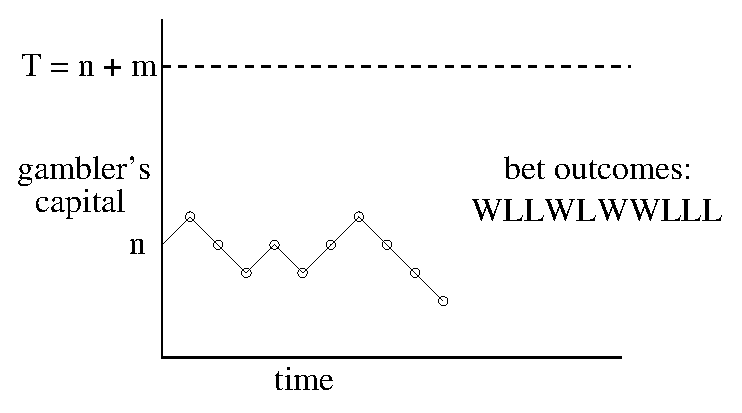
\includegraphics[height=2.5in]{walk1}}
  \caption{A graph of the gambler's capital versus time for one
    possible sequence of bet outcomes.  At each time step, the graph
    goes up with probability $p$ and down with probability $1-p$.  The
    gambler continues betting until the graph reaches either 0 or $T$.
    If he starts with \$$n$, his intended profit is \$$m$ where
    $T=n+m$.}
  \label{LN12:fig:walk1}
\end{figure}

In an \term{unbiased game}, the individual bets are fair: the gambler
is equally likely to win or lose each bet---that is, $p = 1/2$.  The
gambler is more likely to win if $p>1/2$ and less likely to win if
$p<1/2$; these random walks are called \term{biased}.  We want to
determine the probability that the walk terminates at boundary
$T$---the probability that the gambler wins.  We'll do this in
Section~\ref{prwinwalk_subsec}.  But before we derive the probability,
let's examine what it turns out to be.

\begin{editingnotes}

\textcolor{blue}{Make this a pset problem}

\subsection{The Probability Space}

Each random-walk game corresponds to a path like the one in
Figure~\ref{LN12:fig:walk1} that starts at the point $(n,0)$.  A winning path
never touches the $x$ axis and ends when it first touches the line $y=T$.
Likewise, a losing path never touches the line $y=T$ and ends when it first
touches the $x$ axis.

\textcolor{red}{figure causing errors omitted here}
\iffalse

\setlength{\unitlength}{0.0125in}
%
\begingroup\makeatletter\ifx\SetFigFont\undefined
% extract first six characters in \fmtname
\def\x#1#2#3#4#5#6#7\relax{\def\x{#1#2#3#4#5#6}}%
\expandafter\x\fmtname xxxxxx\relax \def\y{splain}%
\ifx\x\y   % LaTeX or SliTeX?
\gdef\SetFigFont#1#2#3{%
  \ifnum #1<17\tiny\else \ifnum #1<20\small\else
  \ifnum #1<24\normalsize\else \ifnum #1<29\large\else
  \ifnum #1<34\Large\else \ifnum #1<41\LARGE\else
     \huge\fi\fi\fi\fi\fi\fi
  \csname #3\endcsname}%
\else
\gdef\SetFigFont#1#2#3{\begingroup
  \count@#1\relax \ifnum 25<\count@\count@25\fi
  \def\x{\endgroup\@setsize\SetFigFont{#2pt}}%
  \expandafter\x
    \csname \romannumeral\the\count@ pt\expandafter\endcsname
    \csname @\romannumeral\the\count@ pt\endcsname
  \csname #3\endcsname}%
\fi
\fi\endgroup
\begin{picture}(300,175)(0,-10)
\path(40,160)(40,0)
\path(20,40)(300,40)
\dottedline{5}(20,140)(300,140)
\path(40,80)(60,100)(80,80)
	(100,100)(120,120)(140,100)
	(160,120)(180,100)(200,80)
	(220,60)(240,80)(260,100)
	(280,120)(300,140)
\put(0,140){\makebox(0,0)[lb]{\smash{{{\SetFigFont{12}{14.4}{rm}T}}}}}
\put(0,40){\makebox(0,0)[lb]{\smash{{{\SetFigFont{12}{14.4}{rm}0}}}}}
\put(60,20){\makebox(0,0)[lb]{\smash{{{\SetFigFont{12}{14.4}{rm}1}}}}}
\put(80,20){\makebox(0,0)[lb]{\smash{{{\SetFigFont{12}{14.4}{rm}2}}}}}
\put(100,20){\makebox(0,0)[lb]{\smash{{{\SetFigFont{12}{14.4}{rm}3}}}}}
\put(0,80){\makebox(0,0)[lb]{\smash{{{\SetFigFont{12}{14.4}{rm}n}}}}}
\end{picture}
\fi

Any length $k$ path can be characterized by the history of wins and
losses on individual \$1 bets, so we use a length $k$ string of $W$'s
and $L$'s to model a path, and assign probability $p^rq^{k-r}$ to a
string that contains $r$ occurrences of $W$.  The \emph{outcomes} in
our sample space will be precisely those string corresponding to
winning or losing walks, that is, when $r = 2k$.

What about the infinite walks in which the gambler plays forever, neither
reaching his target nor going bankrupt?  A recitation problem will show the
probability of playing forever is zero, so we don't need to include any
such outcomes in our sample space.

As a sanity check on this definition of the probability space, you
should verify that the sum of these outcome probabilities is one.

\iffalse
To do this, we let $X$ be any string of $W$'s and $L$'s, and let $[X]$ be
the event consisting of the outcomes that begin with $X$.  If $X$ itself
is not an outcome but begins with an outcome, then $[X] = \emptyset$ so
$\pr{[X]} = 0$.  On the other hand, if no prefix of $X$ is an outcome,
then it's easy to verify by induction on $k$ that $\pr{[X]} = p^rq^{k-r}$.
length $k$
\fi

\end{editingnotes}

%\subsection{The Probability of Winning}

%\subsubsection{The Unbiased Game}

Let's begin by supposing the gambler plays an unbiased game starting
with \$$100$ and will play until he goes broke or reaches a target of
$200$ dollars.  Since he starts equidistant from his target and
bankruptcy in this case, it's clear by symmetry that his probability
of winning is 1/2.

We'll show below that starting with $n$ dollars and aiming for a
target of $T \geq n$ dollars, the probability the gambler reaches his
target before going broke is $n/T$.  For example, suppose he wants to
win the same \$100, but instead starts out with \$500.  Now his
chances are pretty good: the probability of his making the 100 dollars
is $5/6$.  And if he started with one million dollars still aiming to
win \$100 dollars he almost certain to win: the probability is $1M/(1M
+ 100) > .9999$.

So in the unbiased game, the larger the initial stake relative to the
target, the higher the probability the gambler will win, which makes
some intuitive sense.  But note that although the gambler now wins
nearly all the time, when he loses, he loses \emph{big}. Bankruptcy
costs him \$1M, while when he wins, he wins only \$100.  The gambler's
average win remains zero dollars, which is what you'd expect when
making fair bets.

Another useful way to describe this scenario is as a game between two
players.  Say Albert starts with \$500, and Eric starts with \$100.
They flip a fair coin, and every time a Head appears, Albert wins \$1
from Eric, and vice versa for Tails.  They play this game until one
person goes bankrupt.  This problem is identical to the Gambler's Ruin
problem with $n=500$ and $T=100+500=600$.  The probability of Albert
winning is $500/600 = 5/6$.\iffalse , namely, the ratio of his wealth
to the combined wealth.  Eric's chance of winning is $1/6$.\fi

%\subsubsection{The Biased Game}

Now suppose instead that the gambler chooses to play roulette in an
American casino, always betting \$1 on red.  Because the casino puts
two green numbers on its roulette wheels, the probability of winning a
single bet is \iffalse 18/38, which is just\fi a little less than 1/2.
The casino has an advantage, but the bets are close to fair, and you
might expect that starting with \$500, the gambler has a reasonable
chance of winning \$100---the 5/6 probability of winning in the
unbiased game surely gets reduced, but perhaps not too drastically.

This mistaken intuition is how casinos stay in business.  In fact, the
gambler's odds of winning \$100 by making \$1 bets against the
"slightly" unfair roulette wheel are less than 1 in 37,000.  If that's
surprising to you, it only gets weirder from here: 1 in 37,000 is in
fact an upper bound on the gambler's chance of winning
\emph{regardless of his starting stake}.  Whether he starts with
\$5000 or \$5 billion, he still has almost no chance of winning!

\subsection{The Probability of Avoiding Ruin}\label{prwinwalk_subsec}

We will determine the probability that the gambler wins using an idea
of Pascal's dating back to the beginnings of the subject of
probability.

Pascal viewed the walk as a two-player game between Albert and Eric as
described above.  Albert starts with a stack of $n$ chips and Eric
starts with a stack of $m = T-n$ chips.  At each bet, Albert wins
Eric's top chip with probability $p$ and loses his top chip to Eric
with probability $q \eqdef 1-p$.  They play this game until one
person goes bankrupt.

Pascal's ingenious idea was to alter the worth of the chips to make
the game fair regardless of $p$.  Specifically, Pascal assigned
Albert's bottom chip a worth of $r \eqdef q/p$ and then assigned
successive chips \emph{up} his stack worths equal to
$r^{2},r^{3},\dots$ up to his top chip with worth $r^n$.  Eric's top
chip gets assigned worth $r^{n+1}$, and the successive chips
\emph{down} his stack are worth $r^{n+2},r^{n+3},\dots$ down to
his bottom chip worth $r^{n+m}$.

The expected payoff of Albert's first bet is worth
\[
r^{n+1}\cdot p - r^n\cdot q
   = \paren{r^n \cdot \frac{q}{p}} \cdot p - r^n\cdot q = 0.
\]
so this assignment makes the first bet a fair one in terms of worth.
Moreover, whether Albert wins or loses the bet, the successive chip
worths counting up Albert's stack and then down Eric's remain
$r,r^2,\dots,r^n,\dots,r^{n+m}$, ensuring by the same reasoning that
every bet has fair worth.  So, Albert's expected worth at the end of
the game is the sum of the expectations of the worth of each bet,
which is 0.\footnote{Here we're legitimately appealing to infinite
  linearity, since the payoff amounts remain bounded independent of
  the number of bets.}

When Albert wins all of Eric's chips his total gain is worth
\[
\sum_{i=n+1}^{n+m} r^i,
\]
and when he loses all his chips to Eric, his total loss is worth
$\sum_{i=1}^n r^i$.  Letting $w_n$ be Albert's probability of winning,
we now have
\[
0 = \expect{\text{worth of Albert's payoff}} =
 w_n \sum_{i=n+1}^{n+m} r^i - (1-w_n)\sum_{i=1}^n r^i.
\]
In the truly fair game when $r=1$, we have $0 = mw_n - n(1-w_n)$, so
$w_n = n/(n+m)$, as claimed above.

In the biased game with $r\neq 1$, we have
\[
0 =   r \cdot \frac{r^{n+m} - r^{n}}{r-1} \cdot w_n
        - r \cdot \frac{r^{n}-1}{r-1}\cdot (1-w_n).
\]
Solving for $w_n$ gives
\begin{equation}\label{LN12:wnsol}
w_n = \frac{r^n-1}{r^{n+m} -1} = \frac{r^n-1}{r^{T} -1}
\end{equation}

We have now proved
\begin{theorem}\label{thm:gamblerruin}
  In the Gambler's Ruin game with initial capital, $n$, target, $T$,
  and probability $p$ of winning each individual bet,
\begin{equation}\label{eq:gamblerruin}
\pr{\text{the gambler wins}} =
\begin{cases}
 \dfrac{n}{T} & \text{ for } p = \dfrac{1}{2},\\
              &   \\
 \dfrac{r^n-1}{r^{T} -1} & \text{ for } p \neq \dfrac{1}{2},
\end{cases}
\end{equation}
where $r \eqdef q/p$.
\end{theorem}

\subsection{A Recurrence for the Probability of Winning}

Fortunately, you don't need to be as ingenuious Pascal in order to
handle Gambler's Ruin, because linear recurrences offer a methodical
approach the basic problems.

The probability that the gambler wins is a function of his initial
capital, $n$, his target, $T \geq n$, and the probability, $p$, that
he wins an individual one dollar bet.  For fixed $p$ and $T$, let
$w_n$ be the gambler's probability of winning when his initial
capital is $n$ dollars.  For example, $w_0$ is the probability that
the gambler will win given that he starts off broke and $w_T$ is the
probability he will win if he starts off with his target amount, so
clearly
\begin{align}
w_0 & = 0,\label{LN12:w0}\\
w_T & = 1. \label{LN12:wT}
\end{align}

Otherwise, the gambler starts with $n$ dollars, where $0 < n < T$.
Now suppose the gambler wins his first bet.  In this case, he is left
with $n+1$ dollars and becomes a winner with probability $w_{n+1}$.
On the other hand, if he loses the first bet, he is left with $n-1$
dollars and becomes a winner with probability $w_{n-1}$.  By the Total
Probability Rule, he wins with probability $w_n = p w_{n+1} + q
w_{n-1}$.  Solving for $w_{n+1}$ we have
\begin{equation}\label{LN12:rec1}
w_{n+1} = \frac{w_n}{p} - r w_{n-1}
\end{equation}
where $r$ is $q/p$ as in section~\ref{prwinwalk_subsec}.

This recurrence holds only for $n+1 \leq T$, but there's no harm in
using~\eqref{LN12:rec1} to define $w_{n+1}$ for all $n+1 >1$.  Now, letting
\[
W(x) \eqdef w_0 + w_1x + w_2x^2 + \cdots
\]
be the generating function for the $w_n$, we derive from~\eqref{LN12:rec1}
and~\eqref{LN12:w0} using our generating function methods that
\iffalse
\[
W(x) -\frac{xW(x)}{p} + rx^2W(x) = w_1x,
\]
so
\fi
\begin{equation}\label{LN12:Wx}
W(x) = \frac{w_1x}{rx^2- x/p + 1}.
\end{equation}
But it's easy to check that the denominator factors:
\[
rx^2 - \frac{x}{p} + 1 = (1-x)(1-rx).
\]
Now if $p \neq q$, then using partial fractions we conclude that
\begin{equation}\label{LN12:WAB}
W(x) = \frac{A}{1-x} + \frac{B}{1-rx},
\end{equation}
for some constants $A,B$.  To solve for $A,B$, note that
by~\eqref{LN12:Wx} and~\eqref{LN12:WAB},
\[
w_1 x = A(1-rx) + B(1-x),
\]
so letting $x=1$, we get $A=w_1/(1-r)$, and letting $x=1/r$, we get
$B=w_1/(r-1)$.  Therefore,
\[
W(x) = \frac{w_1}{r-1} \paren{\frac{1}{1-rx} - \frac{1}{1-x}},
\]
which implies
\begin{equation}\label{LN12:withw1}
w_n = w_1\frac{r^n - 1}{r-1}.
\end{equation}
Finally, we can use~\eqref{LN12:withw1} to solve for $w_1$ by letting
$n=T$ to get \iffalse
\[
1=w_T = \frac{w_1}{r-1}\paren{r^T - 1}
\]
so
\fi
\[
w_1= \frac{r - 1}{r^T-1}.
\]
Plugging this value of $w_1$ into~\eqref{LN12:withw1}, we arrive at
the solution:
\[
w_n = \frac{r^n-1}{r^T -1},
\]
matching Pascal's result~\eqref{LN12:wnsol}.

In the unbiased case where $p=q$, we get from~\eqref{LN12:Wx} that
\[
W(x) = \frac{w_1 x}{(1-x)^2},
\]
and again can use partial fractions to match Pascal's
result~\eqref{eq:gamblerruin}.

\iffalse
Our derivation of~(\ref{LN12:wnsol}) ensures that it gives a formula for $w_n$
which satisfies~(\ref{LN12:rec1}) and has the right values at $n=0$ and $n=T$.
Moreover, the values determined by~(\ref{LN12:wnsol}) are the \emph{only ones}
that satisfy~\eqref{LN12:rec1} and the boundary conditions at $0$ and $T$,
though we won't prove this.  This implies that the Gambler's probability
of winning is indeed given by~\eqref{LN12:wnsol}.
\fi

\subsection{A simpler expression for the biased case}
The expression~\eqref{LN12:wnsol} for the probability that the Gambler
wins in the biased game is a little hard to interpret.  There is a
simpler upper bound which is nearly tight when the gambler's starting
capital is large and the game is biased \emph{against} the gambler.
Then $r >1$, both the numerator and denominator
in~\eqref{LN12:wnsol} are positive, and the numerator is smaller.
This implies that
\[
w_n < \frac{r^n}{r^T} = \paren{\frac{1}{r}}^{T-n}
\]
and gives:
\begin{corollary}\label{LN12:biaswincor}
  In the Gambler's Ruin game with initial capital, $n$, target, $T$,
  and probability $p < 1/2$ of winning each individual bet,
\begin{equation}\label{LN12:biaswinsimp}
\pr{\text{the gambler wins}} <  \paren{\frac{1}{r}}^{T-n} %\paren{\frac{p}{1-p}}^{T-n}
\end{equation}
where $r \eqdef q/p > 1$.
\end{corollary}

So the gambler gains his intended profit before going broke with
probability at most $1/r$ raised to the intended profit power.
Notice that this upper bound does not depend on the gambler's starting
capital, but only on his intended profit.  This has the amazing
consequence we announced above: \emph{no matter how much money he
  starts with}, if he makes \$1 bets on red in roulette aiming to win
\$100, the probability that he wins is less than
\[
\paren{\frac{18/38}{20/38}}^{100} = \paren{\frac{9}{10}}^{100} < \frac{1}{37,648}.
\]

The bound~\eqref{LN12:biaswinsimp} decreases exponentially as the
intended profit increases.  So, for example, doubling his intended
profit will square his probability of winning.  In this case, the
probability that the gambler's stake goes up $200$ dollars before he
goes broke playing roulette is at most
\[
(9/10)^{200} = ((9/10)^{100})^2 < \paren{\frac{1}{37,648}}^2,
\]
which is about 1 in 1.4 billion.

\begin{editingnotes}

The odds of winning a little money are not so bad.
Applying the exact formula~\eqref{LN12:wnsol}, we find that the probability
of winning \$10 before losing \$10 is
\[
\frac{\paren{\frac{20/38}{18/38}}^{10} - 1}
              {\paren{\frac{20/38}{18/38}}^{20} - 1}
  = 0.2585\dots.
\]
This is somewhat worse than the 1 in 2 chance in the fair game, but not
dramatically so.

\end{editingnotes}

\subsubsection{Intuition}

Why is the gambler so unlikely to make money when the game is only
slightly biased against him?  To answer this intuitively, we can
identify two forces at work on the gambler's wallet.  First, the
gambler's capital has random upward and downward \emph{swings} from
runs of good and bad luck.  Second, the gambler's capital will have a
steady, downward \emph{drift}, because the negative bias means an
average loss of a few cents on each \$1 bet.  The situation is shown
in Figure~\ref{fig:19P3}.

\begin{editingnotes}

For example, in roulette the gambler wins a dollar with probability $9/19$
and loses a dollar with probability $10/19$.  Therefore, his average
return on each bet is $9/10 - 10/19 = - 1/19 \approx -0.053$ dollars.
That is, on each bet his capital is can be expected to drift downward by a
little over 5 cents.

\end{editingnotes}

Our intuition is that if the gambler starts with, say, a billion
dollars, then he is sure to play for a very long time, so at some
point there should be a lucky, upward swing that puts him \$100 ahead.
But his capital is steadily drifting downward.  If the gambler does
not have a lucky, upward swing early on, then he is doomed.  After his
capital drifts downward by tens and then hundreds of dollars, the size
of the upward swing the gambler needs to win grows larger and larger.
And as the size of the required swing grows, the odds that it occurs
decrease exponentially.  As a rule of thumb, \emph{drift dominates
  swings} in the long term.

\begin{figure}[h]

\graphic{gambler}

\caption{In a biased random walk, the downward drift usually dominates
  swings of good luck.}

\label{fig:19P3}

\end{figure}

\iffalse
\begin{figure}
\centerline{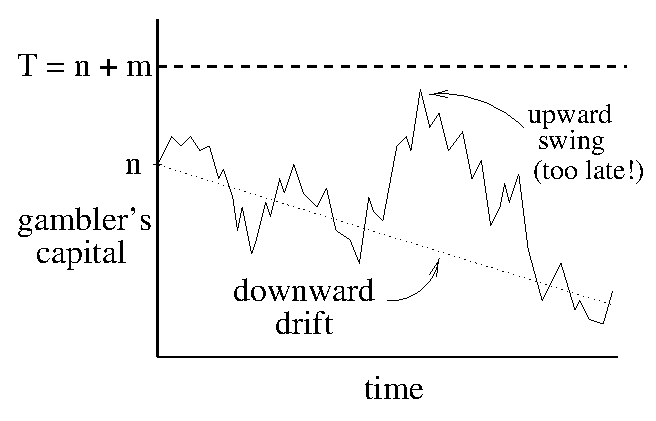
\includegraphics[height=2.5in]{walk2}}
\caption{\em In an unfair game, the gambler's capital swings randomly up
and down, but steadily drifts downward.  If the gambler does not have
a winning swing early on, then his capital drifts downward, and later
upward swings are insufficient to make him a winner.}
\label{LN12:fig:walk2}
\end{figure}
\fi

We can quantify these drifts and swings.  After $k$ rounds for $k \le
\min(m,n)$, the number of wins by our player has a binomial
distribution with parameters $p < 1/2$ and $k$.  His expected win on
any single bet is $p-q = 2p-1$ dollars, so his expected capital is
$n-k(1-2p)$.  Now to be a winner, his actual number of wins must
exceed the expected number by $m+k(1-2p)$.  But from the
formula~\eqref{eq:binom-var}, the binomial distribution has a standard
deviation of only $\sqrt{kp(1-p)}$ .  So for the gambler to win, he
needs his number of wins to deviate by
\[
\frac{m+k(1-2p)}{\sqrt{kp(1-2p)}}=\Theta(\sqrt{k})
\]
times its standard deviation.  In our study of binomial tails, we saw that
this was extremely unlikely.

In a fair game, there is no drift; swings are the only effect.  In the
absence of downward drift, our earlier intuition is correct.  If the
gambler starts with a trillion dollars then almost certainly there
will eventually be a lucky swing that puts him \$100 ahead.

\begin{editingnotes}
If we start with \$10 and play to win only \$10 more, then the difference
between the fair and unfair games is relatively small. We saw that the
probability of winning is $1/2$ versus about $1/4$.  Since swings of \$10
are relatively common, the game usually ends before the gambler's capital
can drift very far.  That is, the game does not last long enough for drift
to dominate the swings.
\end{editingnotes}


\subsection{How Long a Walk?}

Now that we know the probability, $w_n$, that the gambler is a winner in
both fair and unfair games, we consider how many bets he needs on average
to either win or go broke.  A linear recurrence approach works here as well. 

\iffalse
\subsection{Duration of a Biased Walk}

Let $Q$ be the number of bets the gambler makes until the game ends.  

Since the gambler's expected win on any bet is $2p-1$, Wald's
Theorem should tell us that his game winnings, $G$, will have
expectation $\expect{Q}(2p-1)$.  That is,
\begin{equation}\label{LN12:gw}
\expect{G} = (2p-1)\expect{Q},
\end{equation}

In an unbiased game~(\ref{LN12:gw}) is trivially true because both $2p-1$ and
the expected overall winnings, $\expect{G}$, are zero.
On the other hand, in the unfair case, $2p-1 \neq 0$.  Also, we know that
\[
\expect{G} = w_n(T-n) - (1-w_n)n = w_nT-n.
\]
So assuming~(\ref{LN12:gw}), we conclude
\begin{theorem}\label{LN12:ExQthm}
In the biased Gambler's Ruin game with initial capital, $n$, target,
$T$, and probability, $p \neq 1/2$, of winning each bet,
\begin{equation}\label{LN12:ExQ}
\expect{\text{number of bets}} =
\frac{\pr{\text{the gambler wins}}T-n}{2p-1}.
\end{equation}
\end{theorem}

The only problem is that~\eqref{LN12:gw} is not a special case of Wald's
Theorem because $G = \sum_{i=1}^Q G_i$ is not a sum of \emph{nonnegative}
variables: when the gambler loses the $i$th bet, the random variable $G_i$
equals $-1$.  However, this is easily dealt with.\footnote{The random variable
$G_i+1$ is nonnegative, and $\expcond{G_i+1}{Q \geq i} =
\expcond{G_i}{Q\geq i}+1 = 2p$, so by Wald's Theorem
\begin{equation}\label{LN12:G1}
\expect{\sum_{i=1}^Q (G_i+1)}  = 2p\expect{Q}.
\end{equation}
But
\begin{eqnarray}
\expect{\sum_{i=1}^Q (G_i+1)} & = & \expect{\sum_{i=1}^Q G_i + \sum_{i=1}^Q 1}\notag\\
   & = & \expect{(\sum_{i=1}^Q G_i) + Q}\notag\\
   & = & \expect{\sum_{i=1}^Q G_i} + \expect{Q}\notag\\
   & = & \expect{G} + \expect{Q}\label{LN12:GQ}.
\end{eqnarray}
Now combining~(\ref{LN12:G1}) and~(\ref{LN12:GQ}) confirms the truth of our
assumption~(\ref{LN12:gw}).}

\begin{example}
If the gambler aims to profit \$100 playing roulette with $n$ dollars to
start, he can expect to make $((n+100)/37,648 - n)/(2(18/38) - 1) \approx
19n$ bets before the game ends.  So he can enjoy playing for a good while
before almost surely going broke.
\end{example}

\subsection{Duration of an Unbiased Walk}

This time, we need the more general approach of recurrences to handle the
unbiased case.  
\fi

For fixed $p$ and $T$, let $e_n$ be the expected number of bets until
the game ends when the gambler's initial capital is $n$ dollars.
Since the game is over in zero steps if $n=0$ or $T$, the boundary
conditions this time are $e_0=e_T=0$.

Otherwise, the gambler starts with $n$ dollars, where $0 < n < T$.
Now by the conditional expectation rule, the expected number of steps
can be broken down into the expected number of steps given the outcome
of the first bet weighted by the probability of that outcome.  But
after the gambler wins the first bet, his capital is $n+1$, so he can
expect to make another $e_{n+1}$ bets.
That is,
\[
\expcond{e_n}{\text{gambler wins first bet}} = 1 + e_{n+1}.
\]
Similarly, after the gambler loses his first bet, he can expect to
make another $e_{n-1}$ bets:
\[
\expcond{e_n}{\text{gambler loses first bet}} = 1 + e_{n-1}.
\]
So we have
\begin{align*}
e_n & = p\expcond{e_n}{\text{gambler wins first bet}} +
      q\expcond{e_n}{\text{gambler loses first bet}}\\
    & = p(1 + e_{n+1}) +  q(1 + e_{n-1}) =  pe_{n+1} + qe_{n-1} + 1.
\end{align*}
This yields the linear recurrence
\begin{equation}\label{expected-bets-recurrence}
e_{n+1} = \frac{1}{p} e_n - \frac{q}{p} e_{n-1} - \frac{1}{p}.
\end{equation}
\iffalse
For $p = q = 1/2$, this simplifies to
\begin{equation}\label{expected-fair-bets-recurrence}
e_{n+1} = 2e_n - e_{n-1} - 2.
\end{equation}

\fi

The routine solution of this linear recurrence yields:
\begin{theorem}\label{ExQthm}
In the Gambler's Ruin game with initial capital $n$, target
$T$, and probability $p$ of winning each bet,
\begin{equation}\label{expectedbets}
\expect{\text{number of bets}} =
 \begin{cases}
 n(T-n) & \text{ for } p = \dfrac{1}{2},\\
          \\ 
\dfrac{%\frac{r^n - 1}{r^T - 1}%pr{\text{the gambler wins}}
w_n  \cdot T - n}{p-q}
       & \text{ for } p \neq \dfrac{1}{2}\\
       & \text{where } w_n = (r^n - 1)(r^T - 1) = pr{\text{the gambler wins}}.
\end{cases}
\end{equation}
\end{theorem}

In the unbiased case,~\eqref{expectedbets} can be rephrased simply as
\begin{equation}\label{capital.profit}
\expect{\text{number of fair bets}} = \text{initial capital}
\cdot \text{intended profit}.
\end{equation}
For example, if the gambler starts with \$10 dollars and plays until
he is broke or ahead \$10, then $10 \cdot 10 = 100$ bets are required
on average.  If he starts with \$500 and plays until he is broke or
ahead \$100, then the expected number of bets until the game is over
is $500 \times 100 = 50,000$.  This simple
formula~\eqref{capital.profit} cries out for an intuitive proof, but
we have not found one (where are you, Pascal?).

\iffalse

\textcolor{blue}{Below is my try at the suggestion of Santosh and Adam
  Kalai for an example requiring a Pairwise \emph{Uncorrellated}
  Sampling Theorem.  But I don''t think this goes anywhere.}

\subsection{Fluctuations in an Unbiased Walk}

Let's consider the probability that the game ends within $k$ flips.  This
number is awkward to calculate explicitly, but we will be able to estimate
it using our methods for estimating expected deviation from the mean.

Let $C_k$ be the gamblers capital after $k$ flips.  That is,
\[
C_k \eqdef n + \sum_{i=1}^k G_i.
\]
In the unbiased case, the expected win on one flip is zero, so since $C_k$
is the sum of variables which have expectation 0, it follows that
$\expect{C_k} = 0$.  What about $\variance{C_k}$?  We will prove that
\begin{equation}\label{LN12:sumvarg}
\variance{C_k} = \sum_{i=1}^k \variance{G_i}.
\end{equation}

Note that for $i \neq j$, $G_i$ and $G_j$ are not independent, and so we
cannot appeal to pairwise independent additivity of variance to
prove~(\ref{LN12:sumvarg}).  For example, if $G_i = 0$, then the game has
stopped before the $i$th flip, so if $j > i$, then $G_j = 0$.  On the
other hand, the probability that $G_j = 0$ is less than one, because there
is some positive probability that the game will continue for more than $j$
flips (except for the degenerate case when $n=1 and T=2$).  That is,
\[
\prcond{G_j = 0}{G_i = 0} = 1 > \pr{G_j = 0},
\]
confirming nonindependence.

However, inspection of the proof of pairwise independent additivity of
variance shows that it didn't really require pairwise independence!  The
only property of the variables being added is that they be pairwise
\emph{uncorrelated}:

\begin{definition*}
Random variables $R$ and $S$ are \emph{uncorrelated} iff
\begin{equation}\label{LN12:uncor}
\expect{RS} = \expect{R}\expect{S}.
\end{equation}
\end{definition*}

\begin{lemma}\label{LN12:Guncor}
For $i \neq j$, $G_i$ and $G_j$ are uncorrelated.
\end{lemma}
\fi

\subsection{Quit While You Are Ahead}

\begin{editingnotes}
label section as optional.
\end{editingnotes}

Suppose that the gambler never quits while he is ahead.  That is, he
starts with $n>0$ dollars, ignores any target $T$, but plays until he
is flat broke.  Call this the \term{unbounded Gambler's ruin} game.
It turns out that if the game is not favorable, that is, $p \leq 1/2$,
the gambler is sure to go broke.  In particular, this holds in an
unbiased game with $p = 1/2$.

\begin{editingnotes}
If the unbounded game is favorable to the gambler, \ie $p>1/2$, then
there is a positive probability that the gambler will play forever,
see Problem~\TBA{insert problem}.
\end{editingnotes}

\begin{lemma}\label{LN12:go broke}
If the gambler starts with one or more dollars and plays a fair
unbounded game, then he will go broke with probability 1.
\end{lemma}

\begin{proof}
If the gambler has initial capital $n$ and goes broke in a game without
reaching a target $T$, then he would also go broke if he were playing and
ignored the target.  So the probability that he will lose if he keeps
playing without stopping at any target $T$ must be at least as large as the
probability that he loses when he has a target $T>n$.

But we know that in a fair game, the probability that he loses is $1 -
n/T$.  This number can be made arbitrarily close to 1 by choosing a
sufficiently large value of $T$.  Hence, the probability of his losing
while playing without any target has a lower bound arbitrarily close to 1,
which means it must in fact be 1.
\end{proof}

So even if the gambler starts with a million dollars and plays a
perfectly fair game, he will eventually lose it all with probability
1.  But there is good news: if the game is fair, he can ``expect'' to
play forever:

\begin{lemma}\label{LN12:play forever}
If the gambler starts with one or more dollars and plays a fair
unbounded game, then his expected number of plays is infinite.
\end{lemma}

\begin{editingnotes}
\begin{proof}
Let $u_n$ be the expected number of bets for the unbounded game
to end with initial capital $n$.  Also, choose any $T \geq n$, and as
above, let $e_n$ be the expected number of bets for the game to end
when the gambler's target is $T$.

\TBA{not completely clear; revise:}

The unbounded game will have a larger expected number of bets compared
to the game with target $T$ because, in addition to the possibility
that the gambler goes broke, in the game with target $T$ there is also
the possibility that the game will end when the gambler reaches his
target.  That is,
\[
u_n \geq e_n.
\]
So by~\eqref{capital.profit},
\[
u_n \geq n(T-n).
\]
But $n \geq 1$, and $T$ can be any number greater than or equal to $n$, so
this lower bound on $u_n$ can be arbitrarily large.  This implies that
$u_n$ must be infinite.

Now by Lemma~\ref{LN12:go broke}, with probability 1, the unbounded game ends
when the gambler goes broke.  So the expected time for the unbounded game
to \emph{end} is the \emph{same} as the expected time for the gambler to
\emph{go broke}.  Therefore, the expected time to go broke is infinite.
\end{proof}
\end{editingnotes}

A proof appears in Problem~\ref{CP_gambler_unfair_forever}.

So even starting with just one dollar, the expected number of plays
before going broke is infinite!  But don't assume this means that the
gambler is \emph{likely} to play for long---there is even a 50\%
chance he will lose the very first bet and go broke right away.

\iffalse In fact, if the game is unfavorable, then
Theorem~\ref{LN12:ExQthm} and Corollary~\ref{LN12:biaswincor} imply
that his expected time to go broke is essentially proportional to his
initial capital, that is, $\Theta(n)$.  \fi

Lemma~\ref{LN12:play forever} says that the gambler can ``expect'' to
play forever, while Lemma~\ref{LN12:go broke} says that he is certain
to go broke.  These facts sound contradictory, but they are sound
consequences of the technical mathematical definition of expectation.
The moral here, as in section~\ref{infinite_expect_sec}, is that naive
intuition is unreliable when it comes to infinite expectation.

%% Gamblers' Ruin Problems %%%%%%%%%%%%%%%%%%%%%%%%%%%%%%%%%%%%%%%%%%%%%%%%%%%%

\begin{problems}
\practiceproblems
\pinput{TP_Biased_Gamblers_Ruin}

\classproblems
\pinput{CP_gambler_unfair_forever}
\pinput{CP_gambler_ruin_recurrences}
\pinput{CP_gambler_fair_expected_time}

\begin{editingnotes}
\homeworkproblems

DRAFT

\pinput{PS_fair_ruin_probability} 
\end{editingnotes}

a%\pinput{PS_drunken_sailor} used in ran_var_chap
\end{problems}


%% Random Walks on Graphs %%%%%%%%%%%%%%%%%%%%%%%%%%%%%%%%%%%%%%%%%%%%%%%%%%%%%
\section{Random Walks on Graphs}\label{Google_sec}

\begin{editingnotes}

\hyperdef{page}{rank}{Random walks on graphs arise in all sorts of
  applications.  One interesting example is Google and page rank, which
  we'll explore in this section.}

\end{editingnotes}

The hyperlink structure of the World Wide Web can be described as a
digraph.  The vertices are the web pages with a directed edge from vertex
$x$ to vertex $y$ if $x$ has a link to $y$.  For example, in the following
graph the vertices $x_1, \ldots, x_n$ correspond to web pages and
$\diredge{x_i}{x_j}$ is a directed edge when page $x_i$ contains a
hyperlink to page $x_j$.

\begin{editingnotes}
Get a decent figure for a web graph:
\end{editingnotes}

\begin{center}
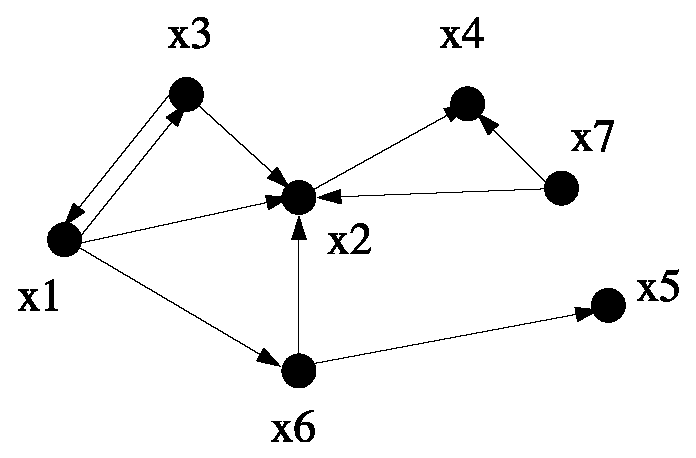
\includegraphics[width = 2in]{randomWalkFigs/webGraph}
\end{center}

The web graph is an enormous graph with trillions of vertices.
\iffalse
At first glance, this graph wouldn't seem to be very interesting.  But\fi
In 1995, two students at Stanford, \index{Page, Larry} Larry Page and
\index{Brin, Sergey} Sergey Brin, realized that the structure of this
graph could be very useful in building a search engine.  Traditional
document searching programs had been around for a long time and they
worked in a fairly straightforward way.  Basically, you would enter
some search terms and the searching program would return all documents
containing those terms.  A relevance score might also be returned for
each document based on the frequency or position that the search terms
appeared in the document.  For example, if the search term appeared in
the title or appeared $100$ times in a document, that document would
get a higher score.  \iffalse
So if an author wanted a document to get a higher
score for certain keywords, he would put the keywords in the title and
make it appear in lots of places.  You can even see this today with
some bogus web sites.\fi

This approach works fine if you only have a few documents that match a
search term.  But on the web, there are many billions of documents and
millions of matches to a typical search.  For example, on May 2, 2012,
a search on Google for `` `Mathematics for Computer Science' text''
gave 482,000 hits!.  Which ones should we look at first?  Just because
a page gets a high keyword score---say because it has ``Mathematics
Mathematics $\dots$ Mathematics'' copied 200 times across the front of
the document---does not make it a great candidate for attention.  The
web is filled with bogus websites that repeat certain words over and
over in order to attract visitors.

\iffalse
One way to get placed high on the list is to pay Google an advertising
fee---and Google gets an enormous revenue stream from these fees.
Of course an early listing is worth a fee only if an advertiser's
target audience is attracted to the listing.  But an audience does get
attracted to Google listings because its ranking method is really good
at determining the most relevant web pages.\fi

Google's enormous market capital in part derives from the revenue it
receives from advertisers paying to appear at the top of search
results.  That top placement would not be worth much if Google's
results were as easy to manipulate keyword frquencies.  Advertisers
pay because Google's ranking method is consistently good at
determining the most relevant web pages.  For example, Google
demonstrated its accuracy in our case by giving first
rank\footnote{First rank for some reason was an early version archived
  at Princeton; the Spring 2010 version on the MIT Open Courseware
  site ranked 4th and 5th.} to our 6.042 text.

So how did Google know to pick our text to be first out of
482,000?...because back in 1995 Larry and Sergey got the idea to allow
the digraph structure of the web to determine which pages are likely
to be the most important.

\subsection{A First Crack at Page Rank}

Looking at the web graph, do you have an idea which vertex/page might
be the best to rank $1$st?  Assume that all the pages match the search
terms for now.  Well, intuitively, we should choose $x_2$, since lots
of other pages point to it.  This leads us to their first idea: try
defining the \term{page rank} of $x$ to be $\text{indegree}(x)$, the
number of links pointing to $x$.  The idea is to think of web pages as
voting for the most important page---the more votes, the better rank.

Unfortunately, there are some problems with this idea.  Suppose you
wanted to have your page get a high ranking.  One thing you could do
is to create lots of dummy pages with links to your page.

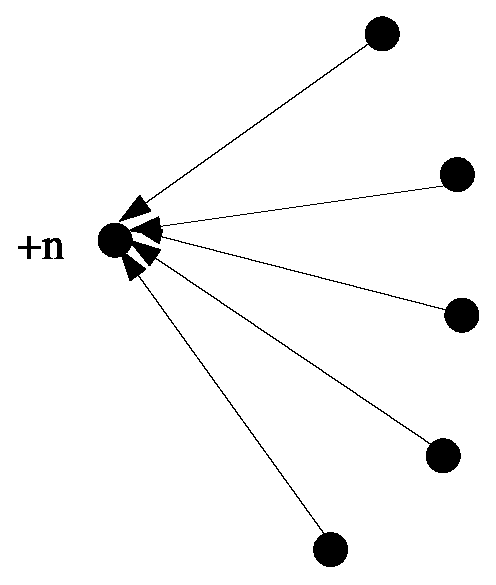
\includegraphics[width = 1.5in]{randomWalkFigs/dummy}

There is another problem---a page could become unfairly influential by
having lots of links to other pages it wanted to hype.

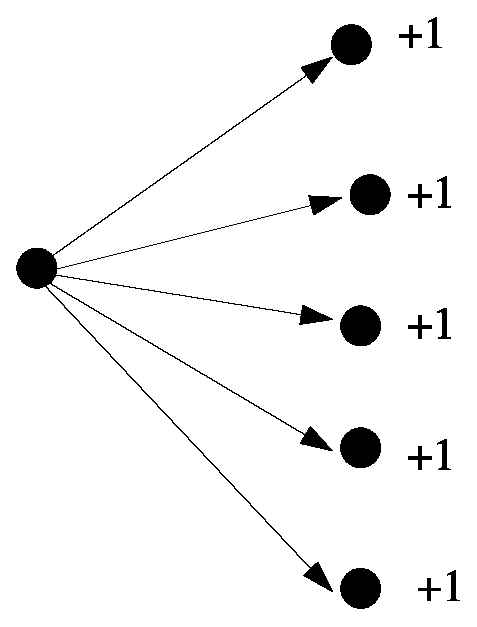
\includegraphics[width = 1.5in]{randomWalkFigs/outDegree}

So this strategy for high ranking would amount to, ``vote early, vote
often,'' which is no good if you want to build a search engine that's
worth paying fees for.  So, admittedly, their original idea was not so
great.  It was better than nothing, but certainly not worth billions of
dollars.

\subsection{Random Walk on the Web Graph}

But then Sergey and Larry thought some more and came up with a couple
of improvements.  Instead of just counting the indegree of a vertex,
they considered the probability of being at each page after a long
random walk on the web graph.  In particular, they decided to model a
user's web experience as following each link on a page with uniform
probability.  For example, if the user is at page $x$, and there are
three links from page $x$, then each link is followed with probability
$1/3$.  More generally, they assigned each edge $x \rightarrow y$ of
the web graph with a probability conditioned on being on page $x$:
\[
\prcond{\text{follow link}\ \diredge{x}{y}}{ \text{at page $x$}} \eqdef
\frac{1}{\outdegr{x}}.
\]
The simulated user experience is then just a \idx{random walk} on the
web graph.

We can also compute the probability of arriving at a particular page, $y$,
by summing over all edges pointing to $y$.  We thus have
\begin{eqnarray}
  \pr{\text{go to $y$}} &=&  \sum_{\text{edges}\ \diredge{x}{y}}
  \prcond{\text{follow link}\ \diredge{x}{y}}{\text{at page $x$}} \cdot
  \pr{\text{at page $x$}} \nonumber\\
  &=& \sum_{\text{edges}\ \diredge{x}{y}} \frac{\pr{\text{at
      $x$}}}{\outdegr{x}} \label{LN12:stepprob}
\end{eqnarray}
For example, in our web graph, we have
\[ \pr{\text{go to $x_4$}} = \frac{\pr{\text{at $x_7$}}}{2} +
\frac{\pr{\text{at $x_2$}}}{1} \ .
\]
One can think of this equation as $x_7$ sending half its probability to
$x_2$ and the other half to $x_4$. The page $x_2$ sends all of its
probability to $x_4$.

There's one aspect of the web graph described thus far that doesn't mesh
with the user experience---some pages have no hyperlinks out.  Under the
current model, the user cannot escape these pages.  In reality, however,
the user doesn't fall off the end of the web into a void of nothingness.
Instead, he restarts his web journey.

To model this aspect of the web, Sergey and Larry added a supervertex to the
web graph and had every page with no hyperlinks point to it.  Moreover,
the supervertex points to every other vertex in the graph, allowing you to
restart the walk from a random place.  For example, below left is a graph
and below right is the same graph after adding the supervertex $x_{N+1}$.

\bigskip\centerline{
  \resizebox{!}{1.3in}{\includegraphics{randomWalkFigs/adjMatrix2}}
  \hspace{2cm}
  \resizebox{!}{1.5in}{\includegraphics{randomWalkFigs/sinkGraph}}
}\bigskip

The addition of the supervertex also removes the possibility that the value
$1/\outdegr{x}$ might involve a division by zero.

\subsection{Stationary Distribution \& Page Rank}

The basic idea of \idx{page rank} is just a stationary distribution over
the web graph,
\begin{editingnotes}
(there are some more details, but this is the main idea)
\end{editingnotes}
so let's define a stationary distribution.

Suppose each vertex is assigned a probability that corresponds, intuitively,
to the likelihood that a random walker is at that vertex at a randomly
chosen time.  We assume that the walk never leaves the vertices in the graph,
so we require that
\begin{equation}\label{LN12:sum1}
\sum_{\text{vertices}\ x} \pr{\text{at $x$}} = 1.
\end{equation}

\begin{definition} An assignment of probabilities to vertices in a digraph
  is a \term{stationary distribution} if for all vertices $x$
\[
\pr{\text{at $x$}} = \pr{\text{go to $x$ at next step}}
\]
\end{definition}  

Sergey and Larry defined their page ranks to be a stationary distribution.
They did this by solving the following system of linear equations: find a
nonnegative number, $\text{PR}(x)$, for each vertex, $x$, such that

\begin{equation}\label{LN12:PReqs}
\text{PR}(x) = \sum_{\text{edges}\ \diredge{y}{x}} \frac{\text{PR}(y)}{\outdegr{y}},
\end{equation}
corresponding to the intuitive equations given in \eqref{LN12:stepprob}.
These numbers must also satisfy the additional constraint corresponding
to~\eqref{LN12:sum1}:
\begin{equation}\label{LN12:sum1PR}
\sum_{\text{vertices}\ x} \text{PR}(x) = 1.
\end{equation}

So if there are $n$ vertices, then equations~\eqref{LN12:PReqs}
and~\eqref{LN12:sum1PR} provide a system of $n+1$ linear equations in the
$n$ variables, $\text{PR}(x)$.  Note that constraint~\eqref{LN12:sum1PR}
is needed because the remaining constraints~\eqref{LN12:PReqs} could be
satisfied by letting $\text{PR}(x)\eqdef 0$ for all $x$, which is useless.

Sergey and Larry were smart fellows, and they set up their page rank
algorithm so it would always have a meaningful solution.  Their addition
of a supervertex ensures there is always a \emph{unique} stationary
distribution.  Moreover, starting from \emph{any} vertex and taking a
sufficiently long random walk on the graph, the probability of being at
each page will get closer and closer to the stationary distribution.  Note
that general digraphs without supervertices may have neither of these
properties: there may not be a unique stationary distribution, and even
when there is, there may be starting points from which the probabilities
of positions during a random walk do not converge to the stationary
distribution.  Examples of this appear in some of the problems below.

\begin{editingnotes}
Here's a note on solving the system of linear constraints, for the
interested reader.

Let $W$ be the $n \times n$ with the entry $w_{ij}$ (in row $i$ and
column $j$) having the value $w_{ij} = 1/\text{outdegree}(x_i)$ if edge
$x_i \rightarrow x_j$ exists, and $w_{ij} = 0$ otherwise.  For example, in
our last example with the 4-vertex graph (including the supervertex), we have
$W$ given by:
\[
\left( \begin{array}{cccc}
    0 & 1 & 0 & 0 \\
    \frac{1}{2} & 0 & \frac{1}{2} & 0 \\
    0 & 0 & 0 & 1\\
    \frac{1}{3} & \frac{1}{3} & \frac{1}{3} & 0 \end{array} \right)
\]

The system of linear equations can now be described by a single matrix
vector product equation $W^T \vec{P} = \vec{P}$, where $W^T$ denotes the
transpose of $W$, and $\vec{P}$ is the column vector of page probabilities
(ranks):
\[\vec{P}\eqdef
\left( \begin{array}{c}
    \text{PR}(x_1) \\
    \text{PR}(x_2) \\
    \vdots \\
    \text{PR}(x_n) \end{array} \right)
\]
So the $j$th entry of the solultion vector, $\vec{P}$, is
\[
\sum_{1\leq i \leq n} w_{ij} \cdot \text{PR}(x_i) =
\sum_{i \mid x_i \rightarrow x_j} \frac{\text{PR}(x_i)}{\text{outdegree}(x_i)},
\]
which is exactly the constraint corresponding to vertex $x_j$
in~\eqref{LN12:PReqs}.

If you have taken a linear algebra or numerical analysis course, you
realize that the vector of page ranks is just the \emph{principle
  eigenvector} of the matrix, $W$, of the web graph!  Once you've had such
a course, these values are easy to compute.  Of course, when you are
dealing with matrices of this size, the problem gets a little more
interesting.

\end{editingnotes}

Now just keeping track of the digraph whose vertices are billions of
web pages is a daunting task.  That's why Google is building power
plants.  Indeed, Larry and Sergey named their system Google after the
number $10^{100}$---which is called a ``googol''---to reflect the
fact that the web graph is so enormous.

Anyway, now you can see how 6.042 ranked first out of 378,000 matches.
Lots of other universities used our notes and presumably have links to the
6.042 open courseware site, and the university sites themselves are
legitimate, which ultimately leads to 6.042 getting a high page rank in
the web graph.

%% Random Walks on Graphs Problems %%%%%%%%%%%%%%%%%%%%%%%%%%%%%%%%%%%%%%%%%%%%
\begin{problems}
\practiceproblems
\pinput{TP_Random_Walks}
\pinput{TP_stable_distribution}
\pinput{TP_uncountable_stationary_distributions}

\classproblems
\pinput{CP_random_walk_stationary_distributions}
\pinput{CP_stationary_distribution}
\pinput{CP_uniform_stationary}
\pinput{CP_simple_google_graph}

\homeworkproblems
\pinput{PS_random_walk_strongly_connected}

\examproblems
\pinput{FP_uniform_stationary_distribution}

\end{problems}
\begin{editingnotes}
CONCLUSION?
\end{editingnotes}
\endinput
 %walks on line & graphs, google rank

\chapter{Random Variables}\label{ran_var_chap}

%% Introduction %%%%%%%%%%%%%%%%%%%%%%%%%%%%%%%%%%%%%%%%%%%%%%%%%%%%%%%%%%%%%%%

So far we focused on probabilities of \idx{events} ---that you win the
Monty Hall game; that you have a rare medical condition, given that
you tested positive; \dots.  Now we focus on quantitative questions:
\emph{How many} contestants must play the Monty Hall game until one of
them finally wins? \dots {\em How long} will this condition last?
{\em How much} will I lose playing silly Math games all day?  Random
variables are the mathematical tool for addressing such questions, and
in this chapter we work out their basic properties, especially
properties of their \term{mean} or \emph{\idx{expected value}}.

%% Random Variables %%%%%%%%%%%%%%%%%%%%%%%%%%%%%%%%%%%%%%%%%%%%%%%%%%%%%%%%%%%
\hyperdef{random}{vars}{\section{Random Variable Examples}}\label{ran_var_examples_sec}

\begin{definition}
  A \term{random variable}, $R$, on a probability space is a total function
  whose domain is the sample space.
\end{definition}
The codomain of $R$ can be anything, but will usually be a subset of
the real numbers.  Notice that the name ``random variable'' is a
misnomer; random variables are actually functions!

For example, suppose we toss three independent, unbiased coins.  Let
$C$ be the number of heads that appear.  Let $M = 1$ if the three
coins come up all heads or all tails, and let $M = 0$ otherwise.  Now
every outcome of the three coin flips uniquely determines the values
of $C$ and $M$.  For example, if we flip heads, tails, heads, then $C
= 2$ and $M = 0$.  If we flip tails, tails, tails, then $C = 0$ and $M
= 1$.  In effect, $C$ counts the number of heads, and $M$ indicates
whether all the coins match.

Since each outcome uniquely determines $C$ and $M$, we can regard them
as functions mapping outcomes to numbers.  For this experiment, the
sample space is:
\begin{eqnarray*}
\sspace & = & \set{ HHH, HHT, HTH, HTT, THH, THT, TTH, TTT }.
\end{eqnarray*}
Now $C$ is a function that maps each outcome in the sample space to a 
number as follows:
\[
\begin{array}{rclcrcl}
C(HHH) & = & 3 & \quad & C(THH) & = & 2 \\
C(HHT) & = & 2 & \quad & C(THT) & = & 1 \\
C(HTH) & = & 2 & \quad & C(TTH) & = & 1 \\
C(HTT) & = & 1 & \quad & C(TTT) & = & 0.
\end{array}
\]
Similarly, $M$ is a function mapping each outcome another way:
\[
\begin{array}{rclcrcl}
M(HHH) & = & 1 & \quad & M(THH) & = & 0 \\
M(HHT) & = & 0 & \quad & M(THT) & = & 0 \\
M(HTH) & = & 0 & \quad & M(TTH) & = & 0 \\
M(HTT) & = & 0 & \quad & M(TTT) & = & 1.
\end{array}
\]
So $C$ and $M$ are \idx{random variables}.

\subsection{Indicator Random Variables}

An \term{indicator random variable} is a random variable that maps every
outcome to either 0 or 1.  These are also called \term{Bernoulli
  variables}.  The random variable $M$ is an example.  If all three coins
match, then $M=1$; otherwise, $M = 0$.

Indicator random variables are closely related to events.  In
particular, an indicator partitions the sample space into those
outcomes mapped to 1 and those outcomes mapped to 0.  For example, the
indicator $M$ partitions the sample space into two blocks as follows:
\[
\underbrace{HHH \quad TTT}_{\text{$M = 1$}} \quad
\underbrace{HHT \quad HTH \quad HTT \quad
        THH \quad THT \quad TTH}_{\text{$M = 0$}}.
\]

In the same way, an event, $E$, partitions the sample space into those
outcomes in $E$ and those not in $E$.  So $E$ is naturally associated with
an indicator random variable, \index{$I_E$, indicator for event $E$}
$I_E$, where $I_E(p) = 1$ for outcomes $p \in E$ and $I_E(p) = 0$ for
outcomes $p \notin E$.  Thus, $M=I_F$ where $F$ is the event that all
three coins match.

\subsection{Random Variables and Events}

There is a strong relationship between events and more general random
variables as well.  A random variable that takes on several values
partitions the sample space into several blocks.  For example, $C$
partitions the sample space as follows:
\[
\underbrace{TTT}_{\text{$C = 0$}} \quad
\underbrace{TTH \quad THT \quad HTT}_{\text{$C = 1$}} \quad
\underbrace{THH \quad HTH \quad HHT}_{\text{$C = 2$}} \quad
\underbrace{HHH}_{\text{$C = 3$}}.
\]
Each block is a subset of the sample space and is therefore
an event.  Thus, we can regard an equation or inequality involving a
random variable as an event.  For example, the event that $C = 2$
consists of the outcomes $THH$, $HTH$, and $HHT$.  The event $C \leq
1$ consists of the outcomes $TTT$, $TTH$, $THT$, and $HTT$.

Naturally enough, we can talk about the probability of events defined
by properties of random variables.  For example, 
\begin{eqnarray*}
\pr{C = 2}
        & = &   \pr{THH} + \pr{HTH} + \pr{HHT} \\
        & = &   \frac{1}{8} + \frac{1}{8} + \frac{1}{8} =  \frac{3}{8}.
\end{eqnarray*}

\begin{editingnotes}

As another example:
\begin{eqnarray*}
\pr{M = 1}
        & = &   \pr{TTT} + \pr{HHH}\\
        & = &   \frac{1}{8} + \frac{1}{8} =    \frac{1}{4}.
\end{eqnarray*}

\subsection{Conditional Probability}

Mixing conditional probabilities and events involving random variables
creates no new difficulties.  For example, $\prcond{C \geq 2}{M = 0}$
is the probability that at least two coins are heads ($C \geq 2$),
given that not all three coins are the same ($M = 0$).  We can compute
this probability using the definition of conditional probability:
\begin{eqnarray*}
\prcond{C \geq 2}{M = 0}
        & = &   \frac{\pr{[C \geq 2] \intersect [M = 0]}}{\pr{M = 0}} \\
        & = &   \frac{\pr{\set{THH, HTH, HHT}}}
                        {\pr{\set{THH, HTH, HHT, HTT, THT, TTH }}} \\
        & = &   \frac{3/8}{6/8} = \frac{1}{2}.
\end{eqnarray*}
The expression $[C \geq 2] \intersect [M = 0]$ on the first line may look odd;
what is the set operation $\intersect$ doing between an inequality and an
equality?  But recall that, in this context, $[C \geq 2]$ and $[M = 0]$
are \emph{events}, namely, \emph{sets} of outcomes.

\end{editingnotes}

\subsection{Independence}

The notion of independence carries over from events to random variables as
well.  Random variables $R_1$ and $R_2$ are \index{independent random
  variables} \emph{independent} iff for all $x_1$ in the codomain of
$R_1$, and $x_2$ in the codomain of $R_2$, we have:
\[
\pr{R_1 = x_1 \QAND R_2 = x_2}  =  \pr{R_1 = x_1} \cdot \pr{R_2 = x_2}.
\]
As with events, we can formulate independence for random
variables in an equivalent and perhaps more intuitive way: random
variables $R_1$ and $R_2$ are independent if for all $x_1$ and $x_2$
\[
\prcond{R_1 = x_1}{R_2 = x_2}  =  \pr{R_1 = x_1}.
\]
whenever the lefthand conditional probability is defined, that is,
whenever $\pr{R_2 = x_2} > 0$.

As an example, are $C$ and $M$ independent?  Intuitively, the answer
should be ``no''.  The number of heads, $C$, completely determines
whether all three coins match; that is, whether $M = 1$.  But, to
verify this intuition, we must find some $x_1, x_2 \in \reals$
such that:
\[
\pr{C = x_1 \QAND M = x_2} \neq \pr{C = x_1} \cdot \pr{M = x_2}.
\]
One appropriate choice of values is $x_1 = 2$ and $x_2 = 1$.
In this case, we have:
\[
\pr{C = 2 \QAND M = 1} = 0 \neq \dfrac{1}{4} \cdot \dfrac{3}{8} = \pr{M
= 1} \cdot \pr{C = 2}.
\]
The first probability is zero because we never have exactly two heads ($C
= 2$) when all three coins match ($M = 1$).  The other two probabilities
were computed earlier.

On the other hand, let $H_1$ be the indicator variable for event that the
first flip is a Head, so
\[
[H_1 = 1] = \set{HHH, HTH, HHT, HTT}.
\]
Then $H_1$ is independent of $M$, since
\begin{align*}
\pr{M=1} & = 1/4 = \prcond{M=1}{H_1=1} = \prcond{M=1}{H_1=0}\\
\pr{M=0} & = 3/4 = \prcond{M=0}{H_1=1} = \prcond{M=0}{H_1=0}
\end{align*}
This example is an instance of a simple lemma:
\begin{lemma}
  Two events are independent iff their \idx{indicator variables} are
  independent.
\end{lemma}
As with events, the notion of independence generalizes to more than two
random variables.
\begin{definition}
Random variables $R_1, R_2, \dots, R_n$ are \term{mutually independent} iff
\begin{eqnarray*}
\lefteqn{\pr{R_1 = x_1 \QAND R_2 = x_2 \QAND \cdots \QAND R_n = x_n}}\\
        & = & \pr{R_1 = x_1} \cdot \pr{R_2 = x_2} \cdots \pr{R_n = x_n}.
\end{eqnarray*}
for all $x_1, x_2, \dots, x_n$.
\end{definition}

It is a simple exercise to show that the probability that any
\emph{subset} of the variables takes a particular set of values is equal
to the product of the probabilities that the individual variables take
their values.  Thus, for example, if $R_1, R_2, \dots, R_{100}$ are
mutually independent random variables, then it follows that:
\[
\pr{R_1 = 7 \QAND R_7 = 9.1 \QAND R_{23} = \pi} = \pr{R_1 = 7} \cdot
\pr{R_7 = 9.1} \cdot \pr{R_{23} = \pi}.
\]

%% Random Variables Problems %%%%%%%%%%%%%%%%%%%%%%%%%%%%%%%%%%%%%%%%%%%%%%%%%%
%\startclassproblems

%% Probability Distributions %%%%%%%%%%%%%%%%%%%%%%%%%%%%%%%%%%%%%%%%%%%%%%%%%%
\section{Probability Distributions}\label{distributions_sec}

A random variable maps outcomes to values, but random variables that show
up for different spaces of outcomes wind up behaving in much the same way
because they have the same probability of taking any given value.  Namely,
random variables on different probability spaces may wind up having the
same probability density function.

\begin{definition}
Let $R$ be a random variable with codomain $V$.
The \term{probability density function (pdf)} of $R$
is a function $\pdf_R : V \to [0,1]$ defined by:
%
\[
\pdf_R(x) \eqdef \begin{cases}
            \pr{R = x} & \text{if } x \in \range{R},\\
             0 & \text{if } x \notin \range{R}.
           \end{cases}
\]
\end{definition}
%
A consequence of this definition is that
%
\[
\sum_{x \in \range{R}} \pdf_R(x) = 1.
\]
This follows because $R$ has a value for each outcome, so summing the
probabilities over all outcomes is the same as summing over the
probabilities of each value in the range of $R$.

As an example, let's return to the experiment of rolling two fair,
independent dice.  As before, let $T$ be the total of the two rolls.
This random variable takes on values in the set $V = \set{2, 3,
\dots, 12}$.  A plot of the probability density function is shown
below:
%
\begin{center}
\begin{picture}(305,110)(-75,-40)
%\put(-75,-40){\dashbox(305,110)} % bounding box
\put(0,0){\vector(1,0){230}}
\put(0,0){\vector(0,1){70}}
\put(-1,60){\line(1,0){2}}
\put(-15,60){\makebox(0,0){{\small $6/36$}}}
\put(-1,30){\line(1,0){2}}
\put(-15,30){\makebox(0,0){{\small $3/36$}}}
\put(-50,40){\makebox(0,0){$\pdf_R(x)$}}
\put(120,-30){\makebox(0,0){$x \in V$}}
\put(0,0){\framebox(20,10){}}
\put(10,-10){\makebox(0,0){2}}
\put(20,0){\framebox(20,20){}}
\put(30,-10){\makebox(0,0){3}}
\put(40,0){\framebox(20,30){}}
\put(50,-10){\makebox(0,0){4}}
\put(60,0){\framebox(20,40){}}
\put(70,-10){\makebox(0,0){5}}
\put(80,0){\framebox(20,50){}}
\put(90,-10){\makebox(0,0){6}}
\put(100,0){\framebox(20,60){}}
\put(110,-10){\makebox(0,0){7}}
\put(120,0){\framebox(20,50){}}
\put(130,-10){\makebox(0,0){8}}
\put(140,0){\framebox(20,40){}}
\put(150,-10){\makebox(0,0){9}}
\put(160,0){\framebox(20,30){}}
\put(170,-10){\makebox(0,0){10}}
\put(180,0){\framebox(20,20){}}
\put(190,-10){\makebox(0,0){11}}
\put(200,0){\framebox(20,10){}}
\put(210,-10){\makebox(0,0){12}}
\end{picture}
\end{center}
%
The lump in the middle indicates that sums close to 7 are the most
likely.  The total area of all the rectangles is 1 since the dice must
take on exactly one of the sums in $V = \set{2, 3, \dots, 12}$.

A closely-related idea is the \term{cumulative distribution function
(cdf)} for a random variable $R$ whose codomain is real numbers.  This is a
function $\cdf_R : \reals \to [0,1]$ defined by:
%
\[
\cdf_R(x) = \pr{R \leq x}
\]
%
As an example, the cumulative distribution function for the random
variable $T$ is shown below:
%
\begin{center}
\begin{picture}(305,155)(-75,-40)
%\put(-75,-40){\dashbox(305,155)} % bounding box
\put(0,0){\vector(1,0){230}}
\put(0,0){\vector(0,1){115}}
\put(-1,108){\line(1,0){2}}
\put(-15,108){\makebox(0,0){{\small $1$}}}
\put(-1,54){\line(1,0){2}}
\put(-15,54){\makebox(0,0){{\small $1/2$}}}
\put(-15,0){\makebox(0,0){{\small $0$}}}
\put(-50,81){\makebox(0,0){$\cdf_R(x)$}}
\put(120,-30){\makebox(0,0){$x \in V$}}
\put(0,0){\framebox(20,3){}}
\put(10,-10){\makebox(0,0){2}}
\put(20,0){\framebox(20,9){}}
\put(30,-10){\makebox(0,0){3}}
\put(40,0){\framebox(20,18){}}
\put(50,-10){\makebox(0,0){4}}
\put(60,0){\framebox(20,30){}}
\put(70,-10){\makebox(0,0){5}}
\put(80,0){\framebox(20,45){}}
\put(90,-10){\makebox(0,0){6}}
\put(100,0){\framebox(20,63){}}
\put(110,-10){\makebox(0,0){7}}
\put(120,0){\framebox(20,78){}}
\put(130,-10){\makebox(0,0){8}}
\put(140,0){\framebox(20,90){}}
\put(150,-10){\makebox(0,0){9}}
\put(160,0){\framebox(20,99){}}
\put(170,-10){\makebox(0,0){10}}
\put(180,0){\framebox(20,105){}}
\put(190,-10){\makebox(0,0){11}}
\put(200,0){\framebox(20,108){}}
\put(210,-10){\makebox(0,0){12}}
\end{picture}
\end{center}
%
The height of the $i$-th bar in the cumulative distribution function
is equal to the \textit{sum} of the heights of the leftmost $i$ bars
in the probability density function.  This follows from the
definitions of pdf and cdf:
%
\begin{align*}
\cdf_R(x) & = \pr{R \leq x} \\
          & = \sum_{y \leq x} \pr{R = y} \\
          & = \sum_{y \leq x} \pdf_R(y)
\end{align*}

In summary, $\pdf_R(x)$ measures the probability that $R = x$ and
$\cdf_R(x)$ measures the probability that $R \leq x$.  Both the
$\pdf_R$ and $\cdf_R$ capture the same information about the random
variable $R$--- you can derive one from the other ---but sometimes one
is more convenient.  The key point here is that neither the
probability density function nor the cumulative distribution function
involves the sample space of an experiment.

\begin{editingnotes}
Thus, through these
functions, we can study random variables without reference to a
particular experiment.

\end{editingnotes}

We'll now look at three important distributions and some applications.

\subsection{Bernoulli Distribution}

\index{indicator variable} Indicator random variables are perhaps the most
common type because of their close association with events.  The
probability density function of an indicator random variable, $B$, is
always
%
\begin{align*}
\pdf_B(0) & = p \\
\pdf_B(1) & = 1 - p \\
\end{align*}
%
where $0 \leq p \leq 1$.  The corresponding cumulative distribution
function is:
%
\begin{align*}
\cdf_B(0) & = p \\
\cdf_B(1) & = 1
\end{align*}
%
%This is called the \term{Bernoulli distribution}. 
%The number of heads
%flipped on a (possibly biased) coin has a Bernoulli distribution.

\subsection{Uniform Distribution}

A random variable that takes on each possible value with the same
probability is called \term{uniform}.  For example, the probability
density function of a random variable $U$ that is uniform on the set
$\set{1, 2, \dots, N}$ is:
%
\begin{align*}
\pdf_U(k) = \frac{1}{N}
\end{align*}
%
And the cumulative distribution function is:
%
\begin{align*}
\cdf_U(k) = \frac{k}{N}
\end{align*}
%
Uniform distributions come up all the time.  For example, the number
rolled on a fair die is uniform on the set $\set{1, 2, \dots, 6}$.

\subsection{The Numbers Game}\label{bigger_number_subsec}

Let's play a game!  I have two envelopes.  Each contains an integer in
the range $0, 1, \dots, 100$, and the numbers are distinct.  To win
the game, you must determine which envelope contains the larger
number.  To give you a fighting chance, I'll let you peek at the
number in one envelope selected at random.  Can you devise a strategy
that gives you a better than 50\% chance of winning?

For example, you could just pick an envelope at random and guess that
it contains the larger number.  But this strategy wins only 50\% of
the time.  Your challenge is to do better.

So you might try to be more clever.  Suppose you peek in the left
envelope and see the number 12.  Since 12 is a small number, you might
guess that that other number is larger.  But perhaps I'm sort of
tricky and put small numbers in \textit{both} envelopes.  Then your
guess might not be so good!

An important point here is that the numbers in the envelopes may
\textit{not} be random.  I'm picking the numbers and I'm choosing them
in a way that I think will defeat your guessing strategy.  I'll only
use randomization to choose the numbers if that serves \textit{my}
end:  making you lose!

\subsubsection{Intuition Behind the Winning Strategy}

Amazingly, there is a strategy that wins more than 50\% of the time,
regardless of what numbers I put in the envelopes!

Suppose that you somehow knew a number $x$ \textit{between} my lower
number and higher numbers.  Now you peek in an envelope and see one or
the other.  If it is bigger than $x$, then you know you're peeking at
the higher number.  If it is smaller than $x$, then you're peeking at
the lower number.  In other words, if you know a number $x$ between
my lower and higher numbers, then you are certain to win the game.

The only flaw with this brilliant strategy is that you do \textit{not}
know $x$.  Oh well.

But what if you try to \textit{guess} $x$?  There is some probability
that you guess correctly.  In this case, you win 100\% of the time.
On the other hand, if you guess incorrectly, then you're no worse off
than before; your chance of winning is still 50\%.  Combining these
two cases, your overall chance of winning is better than 50\%!

Informal arguments about probability, like this one, often sound
plausible, but do not hold up under close scrutiny.  In contrast, this
argument sounds completely implausible--- but is actually correct!

\subsubsection{Analysis of the Winning Strategy}

For generality, suppose that I can choose numbers from the set
$\set{0, 1, \dots, n}$.  Call the lower number $L$ and the higher
number $H$.

Your goal is to guess a number $x$ between $L$ and $H$.  To avoid
confusing equality cases, you select $x$ at random from among the
half-integers:
%
\[
\set{\frac{1}{2},\ 1\frac{1}{2},\ 2\frac{1}{2},\ \dots,\ n - \frac{1}{2}}
\]
%
But what probability distribution should you use?

The uniform distribution turns out to be your best bet.  An informal
justification is that if I figured out that you were unlikely to pick
some number--- say $50\frac{1}{2}$--- then I'd always put 50 and 51 in
the evelopes.  Then you'd be unlikely to pick an $x$ between $L$ and
$H$ and would have less chance of winning.

After you've selected the number $x$, you peek into an envelope and
see some number $p$.  If $p > x$, then you guess that you're looking
at the larger number.  If $p < x$, then you guess that the other
number is larger.

All that remains is to determine the probability that this strategy
succeeds.  We can do this with the usual four step method and a tree
diagram.

\noindent \textbf{Step 1: Find the sample space. }  You either choose
$x$ too low ($< L$), too high ($> H$), or just right ($L < x < H$).
Then you either peek at the lower number ($p = L$) or the higher
number ($p = H$).  This gives a total of six possible outcomes.
%
\begin{center}
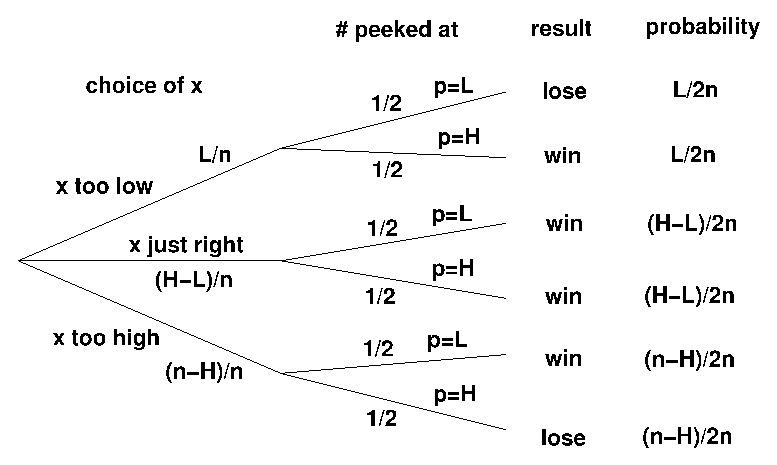
\includegraphics[height=2.5in]{figures/numbers-game}
\end{center}

\noindent \textbf{Step 2: Define events of interest. } The four
outcomes in the event that you win are marked in the tree diagram.

\noindent \textbf{Step 3: Assign outcome probabilities. } First, we
assign edge probabilities.  Your guess $x$ is too low with probability
$L/n$, too high with probability $(n-H)/n$, and just right with
probability $(H-L)/n$.  Next, you peek at either the lower or higher
number with equal probability.  Multiplying along root-to-leaf paths
gives the outcome probabilities.

\noindent \textbf{Step 4: Compute event probabilities. }  The
probability of the event that you win is the sum of the probabilities
of the four outcomes in that event:
%
\begin{align*}
\pr{\text{win}}
    & = \frac{L}{2n} + \frac{H-L}{2n} + \frac{H-L}{2n}  + \frac{n-H}{2n} \\
    & = \frac{1}{2} + \frac{H-L}{2n} \\
    & \geq \frac{1}{2} + \frac{1}{2n}
\end{align*}
%
The final inequality relies on the fact that the higher number $H$ is
at least 1 greater than the lower number $L$ since they are required
to be distinct.

Sure enough, you win with this strategy more than half the time,
regardless of the numbers in the envelopes!  For example, if I choose
numbers in the range $0, 1, \dots, 100$, then you win with probability at
least $\frac{1}{2} + \frac{1}{200} = 50.5\%$.  Even better, if I'm allowed
only numbers in the range $0, \dots, 10$, then your probability of
winning rises to 55\%!  By Las Vegas standards, those are great odds!


\subsection{Binomial Distribution}\label{binomial_distribution_section}

The \term{binomial distribution} plays an important role in Computer
Science as it does in most other sciences.  The standard example of a
random variable with a binomial distribution is the number of heads that
come up in $n$ independent flips of a coin; call this random variable
$H_n$.  If the coin is fair, then $H_n$ has an \textit{unbiased binomial
  density function}:
%
\[
\pdf_{H_n}(k) = \binom{n}{k} 2^{-n}.
\]
%
This follows because there are $\binom{n}{k}$ sequences of $n$ coin
tosses with exactly $k$ heads, and each such sequence has probability
$2^{-n}$.

Here is a plot of the unbiased probability density function
$\pdf_{H_n}(k)$ corresponding to $n = 20$ coins flips.  The most likely
outcome is $k = 10$ heads, and the probability falls off rapidly for
larger and smaller values of $k$.  These falloff regions to the left and
right of the main hump are usually called the \term{tails of the
distribution}.
%
\begin{center}
% GNUPLOT: LaTeX picture
\setlength{\unitlength}{0.240900pt}
\ifx\plotpoint\undefined\newsavebox{\plotpoint}\fi
\sbox{\plotpoint}{\rule[-0.200pt]{0.400pt}{0.400pt}}%
\begin{picture}(1500,900)(0,0)
\font\gnuplot=cmr10 at 10pt
\gnuplot
\sbox{\plotpoint}{\rule[-0.200pt]{0.400pt}{0.400pt}}%
\put(140.0,82.0){\rule[-0.200pt]{4.818pt}{0.400pt}}
\put(120,82){\makebox(0,0)[r]{0}}
\put(1419.0,82.0){\rule[-0.200pt]{4.818pt}{0.400pt}}
\put(140.0,168.0){\rule[-0.200pt]{4.818pt}{0.400pt}}
\put(120,168){\makebox(0,0)[r]{0.02}}
\put(1419.0,168.0){\rule[-0.200pt]{4.818pt}{0.400pt}}
\put(140.0,255.0){\rule[-0.200pt]{4.818pt}{0.400pt}}
\put(120,255){\makebox(0,0)[r]{0.04}}
\put(1419.0,255.0){\rule[-0.200pt]{4.818pt}{0.400pt}}
\put(140.0,341.0){\rule[-0.200pt]{4.818pt}{0.400pt}}
\put(120,341){\makebox(0,0)[r]{0.06}}
\put(1419.0,341.0){\rule[-0.200pt]{4.818pt}{0.400pt}}
\put(140.0,428.0){\rule[-0.200pt]{4.818pt}{0.400pt}}
\put(120,428){\makebox(0,0)[r]{0.08}}
\put(1419.0,428.0){\rule[-0.200pt]{4.818pt}{0.400pt}}
\put(140.0,514.0){\rule[-0.200pt]{4.818pt}{0.400pt}}
\put(120,514){\makebox(0,0)[r]{0.1}}
\put(1419.0,514.0){\rule[-0.200pt]{4.818pt}{0.400pt}}
\put(140.0,601.0){\rule[-0.200pt]{4.818pt}{0.400pt}}
\put(120,601){\makebox(0,0)[r]{0.12}}
\put(1419.0,601.0){\rule[-0.200pt]{4.818pt}{0.400pt}}
\put(140.0,687.0){\rule[-0.200pt]{4.818pt}{0.400pt}}
\put(120,687){\makebox(0,0)[r]{0.14}}
\put(1419.0,687.0){\rule[-0.200pt]{4.818pt}{0.400pt}}
\put(140.0,774.0){\rule[-0.200pt]{4.818pt}{0.400pt}}
\put(120,774){\makebox(0,0)[r]{0.16}}
\put(1419.0,774.0){\rule[-0.200pt]{4.818pt}{0.400pt}}
\put(140.0,860.0){\rule[-0.200pt]{4.818pt}{0.400pt}}
\put(120,860){\makebox(0,0)[r]{0.18}}
\put(1419.0,860.0){\rule[-0.200pt]{4.818pt}{0.400pt}}
\put(140.0,82.0){\rule[-0.200pt]{0.400pt}{4.818pt}}
\put(140,41){\makebox(0,0){0}}
\put(140.0,840.0){\rule[-0.200pt]{0.400pt}{4.818pt}}
\put(465.0,82.0){\rule[-0.200pt]{0.400pt}{4.818pt}}
\put(465,41){\makebox(0,0){5}}
\put(465.0,840.0){\rule[-0.200pt]{0.400pt}{4.818pt}}
\put(790.0,82.0){\rule[-0.200pt]{0.400pt}{4.818pt}}
\put(790,41){\makebox(0,0){10}}
\put(790.0,840.0){\rule[-0.200pt]{0.400pt}{4.818pt}}
\put(1114.0,82.0){\rule[-0.200pt]{0.400pt}{4.818pt}}
\put(1114,41){\makebox(0,0){15}}
\put(1114.0,840.0){\rule[-0.200pt]{0.400pt}{4.818pt}}
\put(1439.0,82.0){\rule[-0.200pt]{0.400pt}{4.818pt}}
\put(1439,41){\makebox(0,0){20}}
\put(1439.0,840.0){\rule[-0.200pt]{0.400pt}{4.818pt}}
\put(140.0,82.0){\rule[-0.200pt]{312.929pt}{0.400pt}}
\put(1439.0,82.0){\rule[-0.200pt]{0.400pt}{187.420pt}}
\put(140.0,860.0){\rule[-0.200pt]{312.929pt}{0.400pt}}
\put(140.0,82.0){\rule[-0.200pt]{0.400pt}{187.420pt}}
\put(140,82){\usebox{\plotpoint}}
\put(140.0,82.0){\rule[-0.200pt]{25.294pt}{0.400pt}}
\put(245.0,82.0){\usebox{\plotpoint}}
\put(245.0,83.0){\rule[-0.200pt]{15.899pt}{0.400pt}}
\put(311.0,83.0){\rule[-0.200pt]{0.400pt}{0.964pt}}
\put(311.0,87.0){\rule[-0.200pt]{15.658pt}{0.400pt}}
\put(376.0,87.0){\rule[-0.200pt]{0.400pt}{3.613pt}}
\put(376.0,102.0){\rule[-0.200pt]{15.899pt}{0.400pt}}
\put(442.0,102.0){\rule[-0.200pt]{0.400pt}{10.600pt}}
\put(442.0,146.0){\rule[-0.200pt]{15.658pt}{0.400pt}}
\put(507.0,146.0){\rule[-0.200pt]{0.400pt}{23.126pt}}
\put(507.0,242.0){\rule[-0.200pt]{15.899pt}{0.400pt}}
\put(573.0,242.0){\rule[-0.200pt]{0.400pt}{38.544pt}}
\put(573.0,402.0){\rule[-0.200pt]{15.899pt}{0.400pt}}
\put(639.0,402.0){\rule[-0.200pt]{0.400pt}{47.939pt}}
\put(639.0,601.0){\rule[-0.200pt]{15.658pt}{0.400pt}}
\put(704.0,601.0){\rule[-0.200pt]{0.400pt}{41.676pt}}
\put(704.0,774.0){\rule[-0.200pt]{15.899pt}{0.400pt}}
\put(770.0,774.0){\rule[-0.200pt]{0.400pt}{16.863pt}}
\put(770.0,844.0){\rule[-0.200pt]{12.527pt}{0.400pt}}
\put(822.0,774.0){\rule[-0.200pt]{0.400pt}{16.863pt}}
\put(822.0,774.0){\rule[-0.200pt]{15.899pt}{0.400pt}}
\put(888.0,601.0){\rule[-0.200pt]{0.400pt}{41.676pt}}
\put(888.0,601.0){\rule[-0.200pt]{15.899pt}{0.400pt}}
\put(954.0,402.0){\rule[-0.200pt]{0.400pt}{47.939pt}}
\put(954.0,402.0){\rule[-0.200pt]{15.658pt}{0.400pt}}
\put(1019.0,242.0){\rule[-0.200pt]{0.400pt}{38.544pt}}
\put(1019.0,242.0){\rule[-0.200pt]{15.899pt}{0.400pt}}
\put(1085.0,146.0){\rule[-0.200pt]{0.400pt}{23.126pt}}
\put(1085.0,146.0){\rule[-0.200pt]{15.658pt}{0.400pt}}
\put(1150.0,102.0){\rule[-0.200pt]{0.400pt}{10.600pt}}
\put(1150.0,102.0){\rule[-0.200pt]{15.899pt}{0.400pt}}
\put(1216.0,87.0){\rule[-0.200pt]{0.400pt}{3.613pt}}
\put(1216.0,87.0){\rule[-0.200pt]{15.899pt}{0.400pt}}
\put(1282.0,83.0){\rule[-0.200pt]{0.400pt}{0.964pt}}
\put(1282.0,83.0){\rule[-0.200pt]{15.658pt}{0.400pt}}
\put(1347.0,82.0){\usebox{\plotpoint}}
\put(1347.0,82.0){\rule[-0.200pt]{22.163pt}{0.400pt}}
\end{picture}
\end{center}
%
In many fields, including Computer Science, probability analyses come down
to getting small bounds on the \idx{tails} of the binomial distribution.
In the context of a problem, this typically means that there is very small
probability that something \emph{bad} happens, which could be a server
or communication link overloading or a randomized algorithm running for an
exceptionally long time or producing the wrong result.

As an example, we can calculate the probability of flipping at most 25
heads in 100 tosses of a fair coin and see that it is very small, namely,
less than 1 in 3,000,000.

\begin{editingnotes}
\textcolor{red}{ calculate that the ratio of the $k-1$st and $k$th terms
  for $k \leq 25$ is less than 1/4(?), so the probability of $< k$ heads
  is less than 1/2 the prob of exactly $k$ heads.  }
\end{editingnotes}

In fact, the tail of the distribution falls off so rapidly that the
probability of flipping exactly 25 heads is nearly twice the
probability of flipping fewer than 25 heads!  That is, the probability
of flipping exactly 25 heads ---small as it is ---is still nearly
twice as large as the probability of flipping exactly 24 heads
\emph{plus} the probability of flipping exactly 23 heads \emph{plus}
\dots the probability of flipping no heads.

\subsubsection{The General Binomial Distribution}

Now let $J$ be the number of heads that come up on $n$ independent
coins, each of which is heads with probability $p$.  Then $J$ has a
\textit{general binomial density function}:
%
\[
\pdf_J(k) = \binom{n}{k} p^k (1-p)^{n-k}.
\]
%
As before, there are $\binom{n}{k}$ sequences with $k$ heads and $n -
k$ tails, but now the probability of each such sequence is $p^k
(1-p)^{n-k}$.

As an example, the plot below shows the probability density function
$\pdf_J(k)$ corresponding to flipping $n=20$ independent coins that
are heads with probabilty $p = 0.75$.  The graph shows that we are
most likely to get around $k = 15$ heads, as you might expect.  Once
again, the probability falls off quickly for larger and smaller values
of $k$.
%
\begin{center}
% GNUPLOT: LaTeX picture
\setlength{\unitlength}{0.240900pt}
\ifx\plotpoint\undefined\newsavebox{\plotpoint}\fi
\sbox{\plotpoint}{\rule[-0.200pt]{0.400pt}{0.400pt}}%
\begin{picture}(1500,900)(0,0)
\font\gnuplot=cmr10 at 10pt
\gnuplot
\sbox{\plotpoint}{\rule[-0.200pt]{0.400pt}{0.400pt}}%
\put(140.0,82.0){\rule[-0.200pt]{4.818pt}{0.400pt}}
\put(120,82){\makebox(0,0)[r]{0}}
\put(1419.0,82.0){\rule[-0.200pt]{4.818pt}{0.400pt}}
\put(140.0,238.0){\rule[-0.200pt]{4.818pt}{0.400pt}}
\put(120,238){\makebox(0,0)[r]{0.05}}
\put(1419.0,238.0){\rule[-0.200pt]{4.818pt}{0.400pt}}
\put(140.0,393.0){\rule[-0.200pt]{4.818pt}{0.400pt}}
\put(120,393){\makebox(0,0)[r]{0.1}}
\put(1419.0,393.0){\rule[-0.200pt]{4.818pt}{0.400pt}}
\put(140.0,549.0){\rule[-0.200pt]{4.818pt}{0.400pt}}
\put(120,549){\makebox(0,0)[r]{0.15}}
\put(1419.0,549.0){\rule[-0.200pt]{4.818pt}{0.400pt}}
\put(140.0,704.0){\rule[-0.200pt]{4.818pt}{0.400pt}}
\put(120,704){\makebox(0,0)[r]{0.2}}
\put(1419.0,704.0){\rule[-0.200pt]{4.818pt}{0.400pt}}
\put(140.0,860.0){\rule[-0.200pt]{4.818pt}{0.400pt}}
\put(120,860){\makebox(0,0)[r]{0.25}}
\put(1419.0,860.0){\rule[-0.200pt]{4.818pt}{0.400pt}}
\put(140.0,82.0){\rule[-0.200pt]{0.400pt}{4.818pt}}
\put(140,41){\makebox(0,0){0}}
\put(140.0,840.0){\rule[-0.200pt]{0.400pt}{4.818pt}}
\put(449.0,82.0){\rule[-0.200pt]{0.400pt}{4.818pt}}
\put(449,41){\makebox(0,0){5}}
\put(449.0,840.0){\rule[-0.200pt]{0.400pt}{4.818pt}}
\put(759.0,82.0){\rule[-0.200pt]{0.400pt}{4.818pt}}
\put(759,41){\makebox(0,0){10}}
\put(759.0,840.0){\rule[-0.200pt]{0.400pt}{4.818pt}}
\put(1068.0,82.0){\rule[-0.200pt]{0.400pt}{4.818pt}}
\put(1068,41){\makebox(0,0){15}}
\put(1068.0,840.0){\rule[-0.200pt]{0.400pt}{4.818pt}}
\put(1377.0,82.0){\rule[-0.200pt]{0.400pt}{4.818pt}}
\put(1377,41){\makebox(0,0){20}}
\put(1377.0,840.0){\rule[-0.200pt]{0.400pt}{4.818pt}}
\put(140.0,82.0){\rule[-0.200pt]{312.929pt}{0.400pt}}
\put(1439.0,82.0){\rule[-0.200pt]{0.400pt}{187.420pt}}
\put(140.0,860.0){\rule[-0.200pt]{312.929pt}{0.400pt}}
\put(140.0,82.0){\rule[-0.200pt]{0.400pt}{187.420pt}}
\put(140,82){\usebox{\plotpoint}}
\put(140.0,82.0){\rule[-0.200pt]{113.705pt}{0.400pt}}
\put(612.0,82.0){\rule[-0.200pt]{0.400pt}{0.482pt}}
\put(612.0,84.0){\rule[-0.200pt]{15.899pt}{0.400pt}}
\put(678.0,84.0){\rule[-0.200pt]{0.400pt}{1.686pt}}
\put(678.0,91.0){\rule[-0.200pt]{12.527pt}{0.400pt}}
\put(730.0,91.0){\rule[-0.200pt]{0.400pt}{5.300pt}}
\put(730.0,113.0){\rule[-0.200pt]{15.899pt}{0.400pt}}
\put(796.0,113.0){\rule[-0.200pt]{0.400pt}{12.768pt}}
\put(796.0,166.0){\rule[-0.200pt]{15.899pt}{0.400pt}}
\put(862.0,166.0){\rule[-0.200pt]{0.400pt}{25.294pt}}
\put(862.0,271.0){\rule[-0.200pt]{12.527pt}{0.400pt}}
\put(914.0,271.0){\rule[-0.200pt]{0.400pt}{38.785pt}}
\put(914.0,432.0){\rule[-0.200pt]{15.899pt}{0.400pt}}
\put(980.0,432.0){\rule[-0.200pt]{0.400pt}{42.157pt}}
\put(980.0,607.0){\rule[-0.200pt]{15.658pt}{0.400pt}}
\put(1045.0,607.0){\rule[-0.200pt]{0.400pt}{25.294pt}}
\put(1045.0,712.0){\rule[-0.200pt]{15.899pt}{0.400pt}}
\put(1111.0,672.0){\rule[-0.200pt]{0.400pt}{9.636pt}}
\put(1111.0,672.0){\rule[-0.200pt]{12.527pt}{0.400pt}}
\put(1163.0,499.0){\rule[-0.200pt]{0.400pt}{41.676pt}}
\put(1163.0,499.0){\rule[-0.200pt]{15.899pt}{0.400pt}}
\put(1229.0,290.0){\rule[-0.200pt]{0.400pt}{50.348pt}}
\put(1229.0,290.0){\rule[-0.200pt]{15.899pt}{0.400pt}}
\put(1295.0,148.0){\rule[-0.200pt]{0.400pt}{34.208pt}}
\put(1295.0,148.0){\rule[-0.200pt]{12.527pt}{0.400pt}}
\put(1347.0,92.0){\rule[-0.200pt]{0.400pt}{13.490pt}}
\put(1347.0,92.0){\rule[-0.200pt]{15.899pt}{0.400pt}}
\put(1413.0,83.0){\rule[-0.200pt]{0.400pt}{2.168pt}}
\put(1413.0,83.0){\rule[-0.200pt]{6.263pt}{0.400pt}}
\end{picture}
\end{center}

\begin{editingnotes}

\subsubsection{Approximating the Binomial Density Function}

Computing the general binomial density function is daunting if not
impossible when $n$ is up in the thousands.  Fortunately, there is an
approximate closed-form formula for this function based on
an approximation for the binomial coefficient.  In the formula, $k$ is
replaced by $\alpha n$ where $\alpha$ is a number between 0 and 1.
%
\begin{lemma}\label{LN12:bincoeff-bound}
\begin{align*}
\binom{n}{\alpha n}
        & \leq \frac{2^{n H(\alpha)}}{\sqrt{2 \pi \alpha (1 - \alpha) n}}
\end{align*}
%
where $H(\alpha)$ is the famous \term{entropy function}:
%
\[
H(\alpha) \eqdef \alpha \log_2 \frac{1}{\alpha} +
                (1 - \alpha) \log_2 \frac{1}{1 - \alpha}
\]
\end{lemma}

%
The graph of $H$ is shown in Figure~\ref{LN12:entropy}.

                                % GNUPLOT: LaTeX picture
\begin{figure}
\setlength{\unitlength}{0.240900pt}
\ifx\plotpoint\undefined\newsavebox{\plotpoint}\fi
\sbox{\plotpoint}{\rule[-0.200pt]{0.400pt}{0.400pt}}%
\begin{picture}(1500,900)(0,0)
  \font\gnuplot=cmr10 at 10pt
  \gnuplot
  \sbox{\plotpoint}{\rule[-0.200pt]{0.400pt}{0.400pt}}%
  \put(220.0,113.0){\rule[-0.200pt]{292.934pt}{0.400pt}}
  \put(220.0,113.0){\rule[-0.200pt]{0.400pt}{184.048pt}}
  \put(220.0,113.0){\rule[-0.200pt]{4.818pt}{0.400pt}}
  \put(198,113){\makebox(0,0)[r]{0}}
  \put(1416.0,113.0){\rule[-0.200pt]{4.818pt}{0.400pt}}
  \put(220.0,266.0){\rule[-0.200pt]{4.818pt}{0.400pt}}
  \put(198,266){\makebox(0,0)[r]{0.2}}
  \put(1416.0,266.0){\rule[-0.200pt]{4.818pt}{0.400pt}}
  \put(220.0,419.0){\rule[-0.200pt]{4.818pt}{0.400pt}}
  \put(198,419){\makebox(0,0)[r]{0.4}}
  \put(1416.0,419.0){\rule[-0.200pt]{4.818pt}{0.400pt}}
  \put(220.0,571.0){\rule[-0.200pt]{4.818pt}{0.400pt}}
  \put(198,571){\makebox(0,0)[r]{0.6}}
  \put(1416.0,571.0){\rule[-0.200pt]{4.818pt}{0.400pt}}
  \put(220.0,724.0){\rule[-0.200pt]{4.818pt}{0.400pt}}
  \put(198,724){\makebox(0,0)[r]{0.8}}
  \put(1416.0,724.0){\rule[-0.200pt]{4.818pt}{0.400pt}}
  \put(220.0,877.0){\rule[-0.200pt]{4.818pt}{0.400pt}}
  \put(198,877){\makebox(0,0)[r]{1}}
  \put(1416.0,877.0){\rule[-0.200pt]{4.818pt}{0.400pt}}
  \put(220.0,113.0){\rule[-0.200pt]{0.400pt}{4.818pt}}
  \put(220,68){\makebox(0,0){0}}
  \put(220.0,857.0){\rule[-0.200pt]{0.400pt}{4.818pt}}
  \put(463.0,113.0){\rule[-0.200pt]{0.400pt}{4.818pt}}
  \put(463,68){\makebox(0,0){0.2}}
  \put(463.0,857.0){\rule[-0.200pt]{0.400pt}{4.818pt}}
  \put(706.0,113.0){\rule[-0.200pt]{0.400pt}{4.818pt}}
  \put(706,68){\makebox(0,0){0.4}}
  \put(706.0,857.0){\rule[-0.200pt]{0.400pt}{4.818pt}}
  \put(950.0,113.0){\rule[-0.200pt]{0.400pt}{4.818pt}}
  \put(950,68){\makebox(0,0){0.6}}
  \put(950.0,857.0){\rule[-0.200pt]{0.400pt}{4.818pt}}
  \put(1193.0,113.0){\rule[-0.200pt]{0.400pt}{4.818pt}}
  \put(1193,68){\makebox(0,0){0.8}}
  \put(1193.0,857.0){\rule[-0.200pt]{0.400pt}{4.818pt}}
  \put(1436.0,113.0){\rule[-0.200pt]{0.400pt}{4.818pt}}
  \put(1436,68){\makebox(0,0){1}}
  \put(1436.0,857.0){\rule[-0.200pt]{0.400pt}{4.818pt}}
  \put(220.0,113.0){\rule[-0.200pt]{292.934pt}{0.400pt}}
  \put(1436.0,113.0){\rule[-0.200pt]{0.400pt}{184.048pt}}
  \put(220.0,877.0){\rule[-0.200pt]{292.934pt}{0.400pt}}
  \put(45,495){\makebox(0,0){$H(\alpha)$}}
  \put(828,23){\makebox(0,0){$\alpha$}}
  \put(220.0,113.0){\rule[-0.200pt]{0.400pt}{184.048pt}}
  \put(232,175){\usebox{\plotpoint}}
  \multiput(232.58,175.00)(0.493,1.845){23}{\rule{0.119pt}{1.546pt}}
  \multiput(231.17,175.00)(13.000,43.791){2}{\rule{0.400pt}{0.773pt}}
  \multiput(245.58,222.00)(0.492,1.746){21}{\rule{0.119pt}{1.467pt}}
  \multiput(244.17,222.00)(12.000,37.956){2}{\rule{0.400pt}{0.733pt}}
  \multiput(257.58,263.00)(0.492,1.573){21}{\rule{0.119pt}{1.333pt}}
  \multiput(256.17,263.00)(12.000,34.233){2}{\rule{0.400pt}{0.667pt}}
  \multiput(269.58,300.00)(0.492,1.401){21}{\rule{0.119pt}{1.200pt}}
  \multiput(268.17,300.00)(12.000,30.509){2}{\rule{0.400pt}{0.600pt}}
  \multiput(281.58,333.00)(0.493,1.250){23}{\rule{0.119pt}{1.085pt}}
  \multiput(280.17,333.00)(13.000,29.749){2}{\rule{0.400pt}{0.542pt}}
  \multiput(294.58,365.00)(0.492,1.272){21}{\rule{0.119pt}{1.100pt}}
  \multiput(293.17,365.00)(12.000,27.717){2}{\rule{0.400pt}{0.550pt}}
  \multiput(306.58,395.00)(0.492,1.142){21}{\rule{0.119pt}{1.000pt}}
  \multiput(305.17,395.00)(12.000,24.924){2}{\rule{0.400pt}{0.500pt}}
  \multiput(318.58,422.00)(0.493,1.052){23}{\rule{0.119pt}{0.931pt}}
  \multiput(317.17,422.00)(13.000,25.068){2}{\rule{0.400pt}{0.465pt}}
  \multiput(331.58,449.00)(0.492,1.056){21}{\rule{0.119pt}{0.933pt}}
  \multiput(330.17,449.00)(12.000,23.063){2}{\rule{0.400pt}{0.467pt}}
  \multiput(343.58,474.00)(0.492,0.970){21}{\rule{0.119pt}{0.867pt}}
  \multiput(342.17,474.00)(12.000,21.201){2}{\rule{0.400pt}{0.433pt}}
  \multiput(355.58,497.00)(0.492,0.970){21}{\rule{0.119pt}{0.867pt}}
  \multiput(354.17,497.00)(12.000,21.201){2}{\rule{0.400pt}{0.433pt}}
  \multiput(367.58,520.00)(0.493,0.853){23}{\rule{0.119pt}{0.777pt}}
  \multiput(366.17,520.00)(13.000,20.387){2}{\rule{0.400pt}{0.388pt}}
  \multiput(380.58,542.00)(0.492,0.841){21}{\rule{0.119pt}{0.767pt}}
  \multiput(379.17,542.00)(12.000,18.409){2}{\rule{0.400pt}{0.383pt}}
  \multiput(392.58,562.00)(0.492,0.841){21}{\rule{0.119pt}{0.767pt}}
  \multiput(391.17,562.00)(12.000,18.409){2}{\rule{0.400pt}{0.383pt}}
  \multiput(404.58,582.00)(0.493,0.734){23}{\rule{0.119pt}{0.685pt}}
  \multiput(403.17,582.00)(13.000,17.579){2}{\rule{0.400pt}{0.342pt}}
  \multiput(417.58,601.00)(0.492,0.712){21}{\rule{0.119pt}{0.667pt}}
  \multiput(416.17,601.00)(12.000,15.616){2}{\rule{0.400pt}{0.333pt}}
  \multiput(429.58,618.00)(0.492,0.755){21}{\rule{0.119pt}{0.700pt}}
  \multiput(428.17,618.00)(12.000,16.547){2}{\rule{0.400pt}{0.350pt}}
  \multiput(441.58,636.00)(0.492,0.669){21}{\rule{0.119pt}{0.633pt}}
  \multiput(440.17,636.00)(12.000,14.685){2}{\rule{0.400pt}{0.317pt}}
  \multiput(453.58,652.00)(0.493,0.616){23}{\rule{0.119pt}{0.592pt}}
  \multiput(452.17,652.00)(13.000,14.771){2}{\rule{0.400pt}{0.296pt}}
  \multiput(466.58,668.00)(0.492,0.625){21}{\rule{0.119pt}{0.600pt}}
  \multiput(465.17,668.00)(12.000,13.755){2}{\rule{0.400pt}{0.300pt}}
  \multiput(478.58,683.00)(0.492,0.582){21}{\rule{0.119pt}{0.567pt}}
  \multiput(477.17,683.00)(12.000,12.824){2}{\rule{0.400pt}{0.283pt}}
  \multiput(490.00,697.58)(0.497,0.493){23}{\rule{0.500pt}{0.119pt}}
  \multiput(490.00,696.17)(11.962,13.000){2}{\rule{0.250pt}{0.400pt}}
  \multiput(503.58,710.00)(0.492,0.539){21}{\rule{0.119pt}{0.533pt}}
  \multiput(502.17,710.00)(12.000,11.893){2}{\rule{0.400pt}{0.267pt}}
  \multiput(515.58,723.00)(0.492,0.539){21}{\rule{0.119pt}{0.533pt}}
  \multiput(514.17,723.00)(12.000,11.893){2}{\rule{0.400pt}{0.267pt}}
  \multiput(527.00,736.58)(0.496,0.492){21}{\rule{0.500pt}{0.119pt}}
  \multiput(527.00,735.17)(10.962,12.000){2}{\rule{0.250pt}{0.400pt}}
  \multiput(539.00,748.58)(0.590,0.492){19}{\rule{0.573pt}{0.118pt}}
  \multiput(539.00,747.17)(11.811,11.000){2}{\rule{0.286pt}{0.400pt}}
  \multiput(552.00,759.58)(0.600,0.491){17}{\rule{0.580pt}{0.118pt}}
  \multiput(552.00,758.17)(10.796,10.000){2}{\rule{0.290pt}{0.400pt}}
  \multiput(564.00,769.58)(0.543,0.492){19}{\rule{0.536pt}{0.118pt}}
  \multiput(564.00,768.17)(10.887,11.000){2}{\rule{0.268pt}{0.400pt}}
  \multiput(576.00,780.59)(0.669,0.489){15}{\rule{0.633pt}{0.118pt}}
  \multiput(576.00,779.17)(10.685,9.000){2}{\rule{0.317pt}{0.400pt}}
  \multiput(588.00,789.59)(0.728,0.489){15}{\rule{0.678pt}{0.118pt}}
  \multiput(588.00,788.17)(11.593,9.000){2}{\rule{0.339pt}{0.400pt}}
  \multiput(601.00,798.59)(0.669,0.489){15}{\rule{0.633pt}{0.118pt}}
  \multiput(601.00,797.17)(10.685,9.000){2}{\rule{0.317pt}{0.400pt}}
  \multiput(613.00,807.59)(0.758,0.488){13}{\rule{0.700pt}{0.117pt}}
  \multiput(613.00,806.17)(10.547,8.000){2}{\rule{0.350pt}{0.400pt}}
  \multiput(625.00,815.59)(0.950,0.485){11}{\rule{0.843pt}{0.117pt}}
  \multiput(625.00,814.17)(11.251,7.000){2}{\rule{0.421pt}{0.400pt}}
  \multiput(638.00,822.59)(0.874,0.485){11}{\rule{0.786pt}{0.117pt}}
  \multiput(638.00,821.17)(10.369,7.000){2}{\rule{0.393pt}{0.400pt}}
  \multiput(650.00,829.59)(1.033,0.482){9}{\rule{0.900pt}{0.116pt}}
  \multiput(650.00,828.17)(10.132,6.000){2}{\rule{0.450pt}{0.400pt}}
  \multiput(662.00,835.59)(1.033,0.482){9}{\rule{0.900pt}{0.116pt}}
  \multiput(662.00,834.17)(10.132,6.000){2}{\rule{0.450pt}{0.400pt}}
  \multiput(674.00,841.59)(1.123,0.482){9}{\rule{0.967pt}{0.116pt}}
  \multiput(674.00,840.17)(10.994,6.000){2}{\rule{0.483pt}{0.400pt}}
  \multiput(687.00,847.59)(1.267,0.477){7}{\rule{1.060pt}{0.115pt}}
  \multiput(687.00,846.17)(9.800,5.000){2}{\rule{0.530pt}{0.400pt}}
  \multiput(699.00,852.59)(1.267,0.477){7}{\rule{1.060pt}{0.115pt}}
  \multiput(699.00,851.17)(9.800,5.000){2}{\rule{0.530pt}{0.400pt}}
  \multiput(711.00,857.60)(1.797,0.468){5}{\rule{1.400pt}{0.113pt}}
  \multiput(711.00,856.17)(10.094,4.000){2}{\rule{0.700pt}{0.400pt}}
  \multiput(724.00,861.61)(2.472,0.447){3}{\rule{1.700pt}{0.108pt}}
  \multiput(724.00,860.17)(8.472,3.000){2}{\rule{0.850pt}{0.400pt}}
  \multiput(736.00,864.61)(2.472,0.447){3}{\rule{1.700pt}{0.108pt}}
  \multiput(736.00,863.17)(8.472,3.000){2}{\rule{0.850pt}{0.400pt}}
  \multiput(748.00,867.61)(2.472,0.447){3}{\rule{1.700pt}{0.108pt}}
  \multiput(748.00,866.17)(8.472,3.000){2}{\rule{0.850pt}{0.400pt}}
  \put(760,870.17){\rule{2.700pt}{0.400pt}}
  \multiput(760.00,869.17)(7.396,2.000){2}{\rule{1.350pt}{0.400pt}}
  \put(773,872.17){\rule{2.500pt}{0.400pt}}
  \multiput(773.00,871.17)(6.811,2.000){2}{\rule{1.250pt}{0.400pt}}
  \put(785,874.17){\rule{2.500pt}{0.400pt}}
  \multiput(785.00,873.17)(6.811,2.000){2}{\rule{1.250pt}{0.400pt}}
  \put(810,875.67){\rule{2.891pt}{0.400pt}}
  \multiput(810.00,875.17)(6.000,1.000){2}{\rule{1.445pt}{0.400pt}}
  \put(797.0,876.0){\rule[-0.200pt]{3.132pt}{0.400pt}}
  \put(834,875.67){\rule{2.891pt}{0.400pt}}
  \multiput(834.00,876.17)(6.000,-1.000){2}{\rule{1.445pt}{0.400pt}}
  \put(822.0,877.0){\rule[-0.200pt]{2.891pt}{0.400pt}}
  \put(859,874.17){\rule{2.500pt}{0.400pt}}
  \multiput(859.00,875.17)(6.811,-2.000){2}{\rule{1.250pt}{0.400pt}}
  \put(871,872.17){\rule{2.500pt}{0.400pt}}
  \multiput(871.00,873.17)(6.811,-2.000){2}{\rule{1.250pt}{0.400pt}}
  \put(883,870.17){\rule{2.700pt}{0.400pt}}
  \multiput(883.00,871.17)(7.396,-2.000){2}{\rule{1.350pt}{0.400pt}}
  \multiput(896.00,868.95)(2.472,-0.447){3}{\rule{1.700pt}{0.108pt}}
  \multiput(896.00,869.17)(8.472,-3.000){2}{\rule{0.850pt}{0.400pt}}
  \multiput(908.00,865.95)(2.472,-0.447){3}{\rule{1.700pt}{0.108pt}}
  \multiput(908.00,866.17)(8.472,-3.000){2}{\rule{0.850pt}{0.400pt}}
  \multiput(920.00,862.95)(2.472,-0.447){3}{\rule{1.700pt}{0.108pt}}
  \multiput(920.00,863.17)(8.472,-3.000){2}{\rule{0.850pt}{0.400pt}}
  \multiput(932.00,859.94)(1.797,-0.468){5}{\rule{1.400pt}{0.113pt}}
  \multiput(932.00,860.17)(10.094,-4.000){2}{\rule{0.700pt}{0.400pt}}
  \multiput(945.00,855.93)(1.267,-0.477){7}{\rule{1.060pt}{0.115pt}}
  \multiput(945.00,856.17)(9.800,-5.000){2}{\rule{0.530pt}{0.400pt}}
  \multiput(957.00,850.93)(1.267,-0.477){7}{\rule{1.060pt}{0.115pt}}
  \multiput(957.00,851.17)(9.800,-5.000){2}{\rule{0.530pt}{0.400pt}}
  \multiput(969.00,845.93)(1.123,-0.482){9}{\rule{0.967pt}{0.116pt}}
  \multiput(969.00,846.17)(10.994,-6.000){2}{\rule{0.483pt}{0.400pt}}
  \multiput(982.00,839.93)(1.033,-0.482){9}{\rule{0.900pt}{0.116pt}}
  \multiput(982.00,840.17)(10.132,-6.000){2}{\rule{0.450pt}{0.400pt}}
  \multiput(994.00,833.93)(1.033,-0.482){9}{\rule{0.900pt}{0.116pt}}
  \multiput(994.00,834.17)(10.132,-6.000){2}{\rule{0.450pt}{0.400pt}}
  \multiput(1006.00,827.93)(0.874,-0.485){11}{\rule{0.786pt}{0.117pt}}
  \multiput(1006.00,828.17)(10.369,-7.000){2}{\rule{0.393pt}{0.400pt}}
  \multiput(1018.00,820.93)(0.950,-0.485){11}{\rule{0.843pt}{0.117pt}}
  \multiput(1018.00,821.17)(11.251,-7.000){2}{\rule{0.421pt}{0.400pt}}
  \multiput(1031.00,813.93)(0.758,-0.488){13}{\rule{0.700pt}{0.117pt}}
  \multiput(1031.00,814.17)(10.547,-8.000){2}{\rule{0.350pt}{0.400pt}}
  \multiput(1043.00,805.93)(0.669,-0.489){15}{\rule{0.633pt}{0.118pt}}
  \multiput(1043.00,806.17)(10.685,-9.000){2}{\rule{0.317pt}{0.400pt}}
  \multiput(1055.00,796.93)(0.728,-0.489){15}{\rule{0.678pt}{0.118pt}}
  \multiput(1055.00,797.17)(11.593,-9.000){2}{\rule{0.339pt}{0.400pt}}
  \multiput(1068.00,787.93)(0.669,-0.489){15}{\rule{0.633pt}{0.118pt}}
  \multiput(1068.00,788.17)(10.685,-9.000){2}{\rule{0.317pt}{0.400pt}}
  \multiput(1080.00,778.92)(0.543,-0.492){19}{\rule{0.536pt}{0.118pt}}
  \multiput(1080.00,779.17)(10.887,-11.000){2}{\rule{0.268pt}{0.400pt}}
  \multiput(1092.00,767.92)(0.600,-0.491){17}{\rule{0.580pt}{0.118pt}}
  \multiput(1092.00,768.17)(10.796,-10.000){2}{\rule{0.290pt}{0.400pt}}
  \multiput(1104.00,757.92)(0.590,-0.492){19}{\rule{0.573pt}{0.118pt}}
  \multiput(1104.00,758.17)(11.811,-11.000){2}{\rule{0.286pt}{0.400pt}}
  \multiput(1117.00,746.92)(0.496,-0.492){21}{\rule{0.500pt}{0.119pt}}
  \multiput(1117.00,747.17)(10.962,-12.000){2}{\rule{0.250pt}{0.400pt}}
  \multiput(1129.58,733.79)(0.492,-0.539){21}{\rule{0.119pt}{0.533pt}}
  \multiput(1128.17,734.89)(12.000,-11.893){2}{\rule{0.400pt}{0.267pt}}
  \multiput(1141.58,720.79)(0.492,-0.539){21}{\rule{0.119pt}{0.533pt}}
  \multiput(1140.17,721.89)(12.000,-11.893){2}{\rule{0.400pt}{0.267pt}}
  \multiput(1153.00,708.92)(0.497,-0.493){23}{\rule{0.500pt}{0.119pt}}
  \multiput(1153.00,709.17)(11.962,-13.000){2}{\rule{0.250pt}{0.400pt}}
  \multiput(1166.58,694.65)(0.492,-0.582){21}{\rule{0.119pt}{0.567pt}}
  \multiput(1165.17,695.82)(12.000,-12.824){2}{\rule{0.400pt}{0.283pt}}
  \multiput(1178.58,680.51)(0.492,-0.625){21}{\rule{0.119pt}{0.600pt}}
  \multiput(1177.17,681.75)(12.000,-13.755){2}{\rule{0.400pt}{0.300pt}}
  \multiput(1190.58,665.54)(0.493,-0.616){23}{\rule{0.119pt}{0.592pt}}
  \multiput(1189.17,666.77)(13.000,-14.771){2}{\rule{0.400pt}{0.296pt}}
  \multiput(1203.58,649.37)(0.492,-0.669){21}{\rule{0.119pt}{0.633pt}}
  \multiput(1202.17,650.69)(12.000,-14.685){2}{\rule{0.400pt}{0.317pt}}
  \multiput(1215.58,633.09)(0.492,-0.755){21}{\rule{0.119pt}{0.700pt}}
  \multiput(1214.17,634.55)(12.000,-16.547){2}{\rule{0.400pt}{0.350pt}}
  \multiput(1227.58,615.23)(0.492,-0.712){21}{\rule{0.119pt}{0.667pt}}
  \multiput(1226.17,616.62)(12.000,-15.616){2}{\rule{0.400pt}{0.333pt}}
  \multiput(1239.58,598.16)(0.493,-0.734){23}{\rule{0.119pt}{0.685pt}}
  \multiput(1238.17,599.58)(13.000,-17.579){2}{\rule{0.400pt}{0.342pt}}
  \multiput(1252.58,578.82)(0.492,-0.841){21}{\rule{0.119pt}{0.767pt}}
  \multiput(1251.17,580.41)(12.000,-18.409){2}{\rule{0.400pt}{0.383pt}}
  \multiput(1264.58,558.82)(0.492,-0.841){21}{\rule{0.119pt}{0.767pt}}
  \multiput(1263.17,560.41)(12.000,-18.409){2}{\rule{0.400pt}{0.383pt}}
  \multiput(1276.58,538.77)(0.493,-0.853){23}{\rule{0.119pt}{0.777pt}}
  \multiput(1275.17,540.39)(13.000,-20.387){2}{\rule{0.400pt}{0.388pt}}
  \multiput(1289.58,516.40)(0.492,-0.970){21}{\rule{0.119pt}{0.867pt}}
  \multiput(1288.17,518.20)(12.000,-21.201){2}{\rule{0.400pt}{0.433pt}}
  \multiput(1301.58,493.40)(0.492,-0.970){21}{\rule{0.119pt}{0.867pt}}
  \multiput(1300.17,495.20)(12.000,-21.201){2}{\rule{0.400pt}{0.433pt}}
  \multiput(1313.58,470.13)(0.492,-1.056){21}{\rule{0.119pt}{0.933pt}}
  \multiput(1312.17,472.06)(12.000,-23.063){2}{\rule{0.400pt}{0.467pt}}
  \multiput(1325.58,445.14)(0.493,-1.052){23}{\rule{0.119pt}{0.931pt}}
  \multiput(1324.17,447.07)(13.000,-25.068){2}{\rule{0.400pt}{0.465pt}}
  \multiput(1338.58,417.85)(0.492,-1.142){21}{\rule{0.119pt}{1.000pt}}
  \multiput(1337.17,419.92)(12.000,-24.924){2}{\rule{0.400pt}{0.500pt}}
  \multiput(1350.58,390.43)(0.492,-1.272){21}{\rule{0.119pt}{1.100pt}}
  \multiput(1349.17,392.72)(12.000,-27.717){2}{\rule{0.400pt}{0.550pt}}
  \multiput(1362.58,360.50)(0.493,-1.250){23}{\rule{0.119pt}{1.085pt}}
  \multiput(1361.17,362.75)(13.000,-29.749){2}{\rule{0.400pt}{0.542pt}}
  \multiput(1375.58,328.02)(0.492,-1.401){21}{\rule{0.119pt}{1.200pt}}
  \multiput(1374.17,330.51)(12.000,-30.509){2}{\rule{0.400pt}{0.600pt}}
  \multiput(1387.58,294.47)(0.492,-1.573){21}{\rule{0.119pt}{1.333pt}}
  \multiput(1386.17,297.23)(12.000,-34.233){2}{\rule{0.400pt}{0.667pt}}
  \multiput(1399.58,256.91)(0.492,-1.746){21}{\rule{0.119pt}{1.467pt}}
  \multiput(1398.17,259.96)(12.000,-37.956){2}{\rule{0.400pt}{0.733pt}}
  \multiput(1411.58,215.58)(0.493,-1.845){23}{\rule{0.119pt}{1.546pt}}
  \multiput(1410.17,218.79)(13.000,-43.791){2}{\rule{0.400pt}{0.773pt}}
  \put(846.0,876.0){\rule[-0.200pt]{3.132pt}{0.400pt}}
\end{picture}
\caption{The Entropy Function}\label{LN12:entropy}
\end{figure}

The upper bound\eqref{LN12:bincoeff-bound} on the binomial coefficient is tight
enough to serve as an excellent approximation.  We'll skip its derivation,
which consists of plugging in Stirling's formula for the factorials in the
binomial coefficient and then simplifying.

Now let's plug this formula into the general binomial density
function.  The probability of flipping $\alpha n$ heads in $n$ tosses
of a coin that comes up heads with probability $p$ is:
%
\begin{equation}\label{LN12:binbnd}
\pdf_J(\alpha n) \leq
        \frac{2^{n H(\alpha)}}{\sqrt{2 \pi \alpha (1 - \alpha) n}} 
        \cdot p^{\alpha n} (1-p)^{(1 - \alpha) n}
\end{equation}
%
This formula is ugly as a bowling shoe, but is useful because it's easy to
evaluate.  For example, suppose we flip a fair coin $n$ times.  What is
the probability of getting \textit{exactly} $\frac{1}{2}n$ heads?
Plugging $\alpha = 1/2$ and $p = 1/2$ and $H(1/2) = 1$ into~\eqref{LN12:binbnd}
gives:
%
\begin{align*}
\pdf_J(\alpha n) & \leq
        \frac{2^{n H(1/2)}}{\sqrt{2 \pi (1/2) (1 - (1/2)) n}}
        \cdot 2^{-n} \\
        & = \sqrt{\frac{2}{\pi n}}
\end{align*}
%
Thus, for example, if we flip a fair coin 100 times, the probability
of getting exactly 50 heads is about $1 / \sqrt{50 \pi} \approx 0.079$
or around 8\%.

\subsection{Approximating the Cumulative Binomial Distribution Function}

Suppose a coin comes up heads with probability $p$.  As before, let
the random variable $J$ be the number of heads that come up on $n$
independent flips.  Then the probability of getting \textit{at most}
$\alpha n$ heads is given by the cumulative binomial distribution function:
%
\begin{equation}\label{LN12:Jsum}
\cdf_J(\alpha n) = \pr{J \leq \alpha n} = \sum_{i = 0}^{\alpha n} \pdf_J(i)
\end{equation}
We can bound this sum by bounding the ratio of successive terms.  This
yields a geometric sum from 0 to $\pdf_J(\alpha n)$ that
bounds~\eqref{LN12:Jsum}.  Then applying the formula for a geometric sum gives
\begin{equation}\label{LN12:nH}
\cdf_J(\alpha n)
         \leq \frac{1 - \alpha}{1 - \alpha / p} \cdot \pdf_J(\alpha n),
\end{equation}
which holds providing $\alpha < p$.  This is all we need, since we already
have the bound~\eqref{LN12:binbnd} for $\pdf_J(\alpha n)$.

It would be awkward to evaluate~\eqref{LN12:nH} with a calculator, but it's
easy to write a program to do it.  So don't look gift blessings in the
mouth before they hatch.  Or something.

As an example, the probability of flipping at most 25 heads in 100
tosses of a fair coin is obtained by setting $\alpha = 1/4$, $p = 1/2$
and $n = 100$:
%
\[
\cdf_J\paren{\frac{n}{4}} \leq \frac{1 - (1/4)}{1 - (1/4) / (1/2)}
                             \cdot \pdf_J\paren{\frac{n}{4}}
                    \leq \frac{3}{2} \cdot 1.913 \cdot 10^{-7}.
\]
%
This says that flipping 25 or fewer heads is extremely unlikely, which
is consistent with our earlier claim that the tails of the binomial
distribution are very small.  In fact, notice that the probability of
flipping \textit{25 or fewer} heads is only 50\% more than the
probability of flipping \textit{exactly 25} heads.  Thus, flipping
exactly 25 heads is twice as likely as flipping any number between 0
and 24!  

\noindent \textbf{Caveat}: The upper bound on $\cdf_J(\alpha n)$ holds
only if $\alpha < p$.  If this is not the case in your problem, then
try thinking in complementary terms; that is, look at the number of
tails flipped instead of the number of heads.  In our example,
the probability of flipping 75 or more heads is the same as
the probability of flipping 25 or fewer tails.  By the above
analysis, this is also extremely small.

\end{editingnotes}

%% Probability Distributions Problems %%%%%%%%%%%%%%%%%%%%%%%%%%%%%%%%%%%%%%%%%
\begin{problems}
\classproblems
\pinput{CP_bigger_number_game}
\pinput{CP_3_random_variables}

\homeworkproblems
\pinput{PS_drunken_sailor}
\end{problems}

%% Average & Expected Value %%%%%%%%%%%%%%%%%%%%%%%%%%%%%%%%%%%%%%%%%%%%%%%%%%%
\hyperdef{great}{expectation}{\section{Average \& Expected
    Value}}\label{expectation_sec} The \term{expectation} of a random
variable is its average value, where each value is weighted according to
the probability that it comes up.  The expectation is also called the
\term{expected value} or the \term{mean} of the random variable.

For example, suppose we select a student uniformly at random from the
class, and let $R$ be the student's quiz score.  Then \index{$\expect{R}$,
  expectation of $R$} $\expect{R}$ is just the class average ---the first
thing everyone wants to know after getting their test back!  For similar
reasons, the first thing you usually want to know about a random variable
is its expected value.

\begin{definition}\label{expdef}
\begin{align}
\expect{R} &\eqdef \sum_{x \in \range{R}} x \cdot \pr{R = x}\label{expsumv}\\
           & = \sum_{x \in \range{R}} x \cdot \pdf_R(x).\notag
\end{align}
\end{definition}

Let's work through an example.  Let $R$ be the number that comes up on a
fair, six-sided die.  Then by~\eqref{expsumv}, the expected value of $R$
is:
%
\begin{align*}
\expect{R}
    & = \sum_{k=1}^6 k \cdot \frac{1}{6} \\
    & = 1 \cdot \frac{1}{6} + 2 \cdot \frac{1}{6} + 3 \cdot \frac{1}{6} +
        4 \cdot \frac{1}{6} + 5 \cdot \frac{1}{6} + 6 \cdot \frac{1}{6} \\
    & = \frac{7}{2}
\end{align*}
%
This calculation shows that the name ``expected value'' is a little
misleading; the random variable might \textit{never} actually take on that
value.  You don't ever expect to roll a $3 \frac{1}{2}$ on an ordinary
die!

There is an even simpler formula for expectation:
\begin{theorem}\label{alt:expdef}
If $R$ is a random variable defined on a sample space, $\sspace$, then
\begin{equation}\label{expsumssp}
\expect{R} = \sum_{\omega \in \sspace} R(\omega) \pr{\omega}
\end{equation}
\end{theorem}
The proof of Theorem~\ref{alt:expdef}, like many of the elementary proofs
about expectation in this chapter, follows by judicious regrouping of terms
in the defining sum~\eqref{expsumv}:
\begin{proof}
\begin{align*}
\expect{R}
    & \eqdef \sum_{x \in \range{R}} x \cdot \pr{R = x} 
                           &\text{(Def~\ref{expdef} of expectation)}\\
    & = \sum_{x \in \range{R}} x \paren{\sum_{\omega \in [R=x]} \pr{\omega}}
              & \text{(def of $\pr{R=x}$)}\\
    & = \sum_{x \in \range{R}} \sum_{\omega \in [R=x]} x \pr{\omega}
             & \text{(distributing $x$ over the inner sum)} \\    
    & = \sum_{x \in \range{R}} \sum_{\omega \in [R=x]} R(\omega) \pr{\omega} 
                &\text{(def of the event $[R=x]$)}\\
    & = \sum_{\omega \in \sspace} R(\omega) \pr{\omega}
\end{align*}
The last equality follows because the events $[R=x]$ for $x \in \range{R}$
partition the sample space, $\sspace$, so summing over the outcomes in
$[R=x]$ for $x \in \range{R}$ is the same as summing over $\sspace$.
\end{proof}

In general, the defining sum~\eqref{expsumv} is better for calculating
expected values and has the advantage that it does not depend on the
sample space, but only on the density function of the random variable.  On
the other hand, the simpler sum over all outcomes~\eqref{expsumssp}is
sometimes easier to use in proofs about expectation.

\subsection{Expected Value of an Indicator Variable}

The \idx{expected value} of an \index{indicator variable} indicator random
variable for an event is just the probability of that event.  \iffalse
(Remember that a random variable $I_A$ is the indicator random variable
for event $A$, if $I_A = 1$ when $A$ occurs and $I_A= 0$ otherwise.)\fi

\begin{lemma}\label{expindic}
If $I_A$ is the indicator random variable for event $A$, then
\[
\expect{I_A} = \pr{A}.
\]
\end{lemma}

\begin{proof}
\begin{align*}
\expect{I_A} 
& =  1 \cdot \pr{I_A = 1} + 0 \cdot \pr{I_A = 0} \\
& = \pr{I_A = 1} \\
& =  \pr{A}. & \text{(def of $I_A$)}
\end{align*}
\end{proof}
For example, if $A$ is the event that a coin
with bias $p$ comes up heads, $\expect{I_A} = \pr{I_A=1} = p$.

\subsection{Conditional Expectation}

Just like event probabilities, expectations can be conditioned on some
event.
\begin{definition}\label{condexpdef} %\begin{theorem}\label{alt:condexpdef} 
The \term{conditional expectation}, $\expcond{R}{A}$, of a random
variable, $R$, given event, $A$, is:
\begin{equation}\label{condexpsumv}
\expcond{R}{A} \eqdef \sum_{r \in \range{R}} r \cdot\prcond{R=r}{A}.
\end{equation}
\end{definition}
In other words, it is the average value of the variable $R$ when values
are weighted by their conditional probabilities given $A$.

For example, we can compute the expected value of a roll of a fair die,
\emph{given}, for example, that the number rolled is at least 4.  We do
this by letting $R$ be the outcome of a roll of the die.  Then
by equation~\eqref{condexpsumv},
\[
\expcond{R}{R \geq 4} = \sum_{i=1}^6 i \cdot \prcond{R=i}{R \ge 4} 
%= \sum_{i=4}^6 i \cdot 1/3 
= 1\cdot 0 + 2\cdot 0 + 3\cdot 0 + 
  4\cdot\tfrac{1}{3} + 5\cdot\tfrac{1}{3} + 6\cdot\tfrac{1}{3} 
= 5.
\]

The power of conditional expectation is that it lets us divide complicated
expectation calculations into simpler cases.  We can find the desired
expectation by calculating the conditional expectation in each simple case
and averaging them, weighing each case by its probability.

For example, suppose that 49.8\% of the people in the world are male and
the rest female ---which is more or less true.  Also suppose the expected
height of a randomly chosen male is $5'\,11''$, while the expected height
of a randomly chosen female is $5'\,5''$.  What is the expected height of a
randomly chosen individual?  We can calculate this by averaging the
heights of men and women.  Namely, let $H$ be the height (in feet) of a
randomly chosen person, and let $M$ be the event that the person is male
and $F$ the event that the person is female.  We have
\begin{align*}
\expect{H} &= \expcond{H}{M} \pr{M} + \expcond{H}{F} \pr{F}\\
&= (5 + 11/12) \cdot 0.498  + (5+ 5/12) \cdot 0.502\\
&= 5.665
\end{align*}
which is a little less that 5'\,8".

The Law of \term{Total Expectation} justifies this method.

\begin{theorem}\label{total_expect} %\label{thm:condexp}
Let $A_1,A_2,\dots$ be a partition of the sample space.  Then
\begin{rul*}[Law of Total Expectation]
\[
\expect{R} = \sum_i \expcond{R}{A_i} \pr{A_i}.
\]
\end{rul*}
\end{theorem}

\begin{proof}
  \begin{align*}
    \expect{R} &\eqdef \sum_{r \in \range{R}} r \cdot \pr{R=r}
                  & \text{(Def~\ref{expdef} of expectation)}\\
    &= \sum_r r \cdot \sum_i \prcond{R=r}{A_i} \pr{A_i}
            & \text{(Law of Total Probability)}\\
    &= \sum_r \sum_i r \cdot \prcond{R=r}{A_i} \pr{A_i}
              & \text{(distribute constant $r$)}\\
    &= \sum_i \sum_r r \cdot \prcond{R=r}{A_i} \pr{A_i}
              & \text{(exchange order of summation)}\\
    &= \sum_i \pr{A_i} \sum_r r \cdot \prcond{R=r}{A_i}
             & \text{(factor constant $\pr{A_i}$)}\\
    &= \sum_i \pr{A_i} \expcond{R}{A_i}.
             & \text{(Def~\ref{condexpdef} of cond.\ expectation)}
  \end{align*}
\end{proof}


\begin{editingnotes}

\subsubsection{Properties of Conditional Expectation}

\textcolor{red}{
Not needed, since pset shows that condexp is an expectation using
the ``relative''probability function  from PS\_conditional\_space.}

\end{editingnotes}

\iffalse

If a random variable is independent of an event, then conditional
expectation given that event coincides with ordinary expectation:
\begin{lemma}\label{RIA}
If $R$ and $I_A$ are independent random variables, then
\[
\expcond{R}{A} = \expect{R}.
\]
\end{lemma}

\begin{proof}
If $R$ and $I_A$ are independent, then
\[
\prcond{R=r}{A} = \prcond{R=r}{I_A=1} = \pr{R=r}
\]
by the definition of independence of random variables, so the righthand
side of equation~\eqref{condexpsumv} for conditional expectation coincides
with the righthand side of the corresponding equation~\eqref{expsumv} for
ordinary expectation.
\end{proof}

Many rules for conditional expectation correspond directly to rules for
ordinary expectation.\iffalse
For example, we can calculate conditional
expectations by summing over outcomes instead of values:
\begin{theorem}\label{alt:condexpdef}
\begin{equation}\label{condexpsumssp}
\expcond{R}{A} = \sum_{\omega \in \sspace} R(\omega) \prcond{w}{A}.
\end{equation}
\end{theorem}
The proof of Theorem~\ref{alt:condexpdef} is essentially the same as the
proof of the corresponding Theorem~\ref{alt:expdef} for ordinary
expectation, so we won't repeat it.\fi

For example, linearity of conditional expectation carries over
with the same proof:
\begin{theorem}\label{condexplin}
For any two random variables $R_1$, $R_2$, constants
$a_1,a_2\in\reals$, and event $A$, 
\[
\expcond{a_1R_1+a_2R_2}{A} = a_1\expcond{R_1}{A} + a_2\expcond{R_2}{A}.
\]
\end{theorem}

Likewise,
\begin{theorem}
For any two \emph{independent} random variables $R_1$, $R_2$, and event, $A$,
\[
\expcond{R_1 \cdot R_2}{A} = \expcond{R_1}{A} \cdot \expcond{R_2}{A}.
\]
\end{theorem}
\fi

\subsection{Mean Time to Failure}\label{mean_time_to_failure_subsec}

A computer program crashes at the end of each hour of use with probability
$p$, if it has not crashed already.  What is the expected time until the
program crashes?

If we let $C$ be the number of hours until the crash, then the answer to
our problem is $\expect{C}$.  Now the probability that, for $i >0$, the
first crash occurs in the $i$th hour is the probability that it does not
crash in each of the first $i-1$ hours and it does crash in the $i$th
hour, which is $(1-p)^{i-1}p$.  So from formula~\eqref{expsumv} for
expectation, we have
\begin{align*}
\expect{C} & = \sum_{i \in \naturals} i \cdot \pr{R=i}\\
           & = \sum_{i \in \naturals^+} i (1-p)^{i-1}p\\
           &= p \sum_{i \in \naturals^+} i (1-p)^{i-1}\\
           &= p\frac{1}{(1-(1-p))^2} & \text{(by~\eqref{sumixi-1})}\\
           &= \frac{1}{p}
\end{align*}


A simple alternative derivation that does not depend on
the formula~\eqref{sumixi-1}
\iffalse
for $\sum_{i \in \naturals^{+}} ix^{i-1}$
\begin{equation}\label{Notes11form}
\sum_{i \in \naturals^{+}} ix^{i-1} =\frac{1}{(1-x)^2}
\end{equation}
\fi (which you remembered, right?) is based on \idx{conditional
  expectation}.  Given that the computer crashes in the first hour, the
expected number of hours to the first crash is obviously 1!  On the other
hand, given that the computer does not crash in the first hour, then the
expected total number of hours till the first crash is the expectation of
one plus the number of additional hours to the first crash.  So,
\[
\expect{C} = p\cdot 1 + (1-p)\expect{C+1} = p + \expect{C} -p\expect{C} +
1 - p,
\]
from which we immediately calculate that $\expect{C} = 1/p$.

\begin{editingnotes}

There is a useful trick for
calculating expectations of nonegative integer valued variables:
\begin{lemma}
If $R$ is a nonegative integer-valued random variable, then:
%
\begin{equation}\label{R>i}
\expect{R} = \sum_{i \in \naturals} \pr{R > i}
\end{equation}
\end{lemma}

\begin{proof}
Consider the sum:
%
\[
\begin{array}{ccccccc}
\pr{R = 1} & + & \pr{R = 2} & + & \pr{R = 3} & + & \cdots \\
           & + & \pr{R = 2} & + & \pr{R = 3} & + & \cdots \\
           &   &            & + & \pr{R = 3} & + & \cdots \\
           &   &            &   &            & + & \cdots
\end{array}
\]
%
The successive columns sum to $1 \cdot \pr{R = 1}$, $2 \cdot \pr{R = 2}$,
$3 \cdot \pr{R = 3}$, \dots.  Thus, the whole sum is equal to:
%
\[
\sum_{i \in \naturals} i \cdot \pr{R = i}
\]
which equals $\expect{R}$ by~\eqref{expsumv}.  On the other hand, the
successive rows sum to $\pr{R > 0}$, $\pr{R > 1}$, $\pr{R > 2}$, \dots.
Thus, the whole sum is also equal to:
%
\[
\sum_{i \in \naturals} \pr{R > i},
\]
%
which therefore must equal $\expect{R}$ as well.
\end{proof}

Now $\pr{C > i}$ is easy to evaluate: a crash happens later than the $i$th
hour iff the system did not crash during the first $i$ hours, which
happens with probability $(1-p)^i$.  Plugging this into~\eqref{R>i} gives:
%
\begin{align*}
\expect{C} & = \sum_{i \in \naturals} (1-p)^i \\
       & = \frac{1}{1 - (1-p)} & \text{(sum of geometric series)}\\
       & = \frac{1}{p}
\end{align*}

The general principle here is well-worth
remembering: if a system fails at each time step with probability $p$,
then the expected number of steps up to the first failure is $1 / p$.

\end{editingnotes}

So, for example, if there is a 1\% chance that the program crashes at
the end of each hour, then the expected time until the program crashes
is $1 / 0.01 = 100$ hours.  

As a further example, suppose a couple really wants to have a baby girl.
For simplicity assume there is a 50\% chance that each child they have is a
girl, and the genders of their children are mutually independent.  If the
couple insists on having children until they get a girl, then how many
baby boys should they expect first?

This is really a variant of the previous problem.  The question, ``How
many hours until the program crashes?'' is mathematically the same as
the question, ``How many children must the couple have until they get
a girl?''  In this case, a crash corresponds to having a girl, so we
should set $p = 1/2$.  By the preceding analysis, the couple
should expect a baby girl after having $1/p = 2$ children.  Since the
last of these will be the girl, they should expect just one boy.

Something to think about: If every couple follows the strategy of having
children until they get a girl, what will eventually happen to the
fraction of girls born in this world?

\subsection{Linearity of Expectation}\label{finlin}

Expected values obey a simple, very helpful rule called
\hyperdef{linearity}{expectation}{\term{Linearity of Expectation}}.  Its
simplest form says that the expected value of a sum of random variables is
the sum of the expected values of the variables.

\begin{theorem}\label{expsum-2}
For any random variables $R_1$ and $R_2$,
\[
\expect{R_1 + R_2} = \expect{R_1} + \expect{R_2}.
\]
\end{theorem}

\begin{proof}
Let $T \eqdef R_1+R_2$.  The proof follows straightforwardly by
rearranging terms in the sum~\eqref{expsumssp}
\begin{align*}
\expect{T} & = \sum_{\omega \in \sspace} T(\omega) \cdot \pr{\omega}
                & \text{(Theorem~\ref{alt:expdef})}\\
        & = \sum_{\omega \in \sspace} (R_1(\omega) + R_2(\omega)) \cdot \pr{\omega}
                         & \text{(def of $T$)}\\
        & = \sum_{\omega \in \sspace} R_1(\omega) \pr{\omega} + 
              \sum_{\omega \in \sspace} R_2(\omega) \pr{\omega} & \text{(rearranging terms)}\\
        & = \expect{R_1} + \expect{R_2}.   & \text{(Theorem~\ref{alt:expdef})}
\end{align*}
\end{proof}

A small extension of this proof, which we leave to the reader, implies
\begin{theorem}[\idx{Linearity of Expectation}]
For random variables $R_1$, $R_2$ and constants $a_1,a_2 \in \reals$,
\[
\expect{a_1R_1 + a_2R_2} = a_1\expect{R_1} + a_2\expect{R_2}.
\]
\end{theorem}
In other words, expectation is a linear function.  A routine induction
extends the result to more than two variables:
\begin{corollary}\label{linexp-k-thm}
For any random variables $R_1, \dots, R_k$ and constants $a_1, \dots, a_k
\in \reals$,
\[
\expect{\sum_{i=1}^k a_iR_i} = \sum_{i=1}^k a_i\expect{R_i}.
\]
\end{corollary}

The great thing about linearity of expectation is that \emph{no
independence is required}.  This is really useful, because dealing with
independence is a pain, and we often need to work with random variables
that are not independent.

\begin{editingnotes}
Even when the random variables \emph{are} independent, we know
from previous experience that proving independence requires a lot of
work.
\end{editingnotes}


\subsubsection{Expected Value of Two Dice}

What is the expected value of the sum of two fair dice?

Let the random variable $R_1$ be the number on the first die, and let
$R_2$ be the number on the second die.  We observed earlier that the
expected value of one die is 3.5.  We can find the expected value of the
sum using linearity of expectation:
\begin{equation*}
\expect{R_1 + R_2} 
 =   \expect{R_1} + \expect{R_2}
 =    3.5 + 3.5
 =    7.
\end{equation*}

Notice that we did \emph{not} have to assume that the two dice were
independent.  The expected sum of two dice is 7, even if they are glued
together (provided each individual die remainw fair after the gluing).
Proving that this expected sum is 7 with a tree diagram would be a bother:
there are 36 cases.  And if we did not assume that the dice were
independent, the job would be really tough!

\subsubsection{The Hat-Check Problem}

There is a dinner party where $n$ men check their hats.  The hats are
mixed up during dinner, so that afterward each man receives a random hat.
In particular, each man gets his own hat with probability $1/n$.  What is
the expected number of men who get their own hat?

Letting $G$ be the number of men that get their own hat, we want to find
the expectation of $G$.  But all we know about $G$ is that the probability
that a man gets his own hat back is $1/n$.  There are many different
probability distributions of hat permutations with this property, so we
don't know enough about the distribution of $G$ to calculate its
expectation directly.  But linearity of expectation makes the problem
really easy.

The trick is to express $G$ as a sum of indicator variables.  In
particular, let $G_i$ be an indicator for the event that the $i$th man
gets his own hat.  That is, $G_i = 1$ if he gets his own hat, and $G_i =
0$ otherwise.  The number of men that get their own hat is the sum of
these indicators:
%
\begin{equation}\label{GG}
G = G_1 + G_2 + \cdots + G_n.
\end{equation}
%
These indicator variables are \textit{not} mutually independent.  For
example, if $n-1$ men all get their own hats, then the last man is
certain to receive his own hat.  But, since we plan to use linearity
of expectation, we don't have worry about independence!

Now since $G_i$ is an indicator, we know $1/n = \pr{G_i=1} = \expect{G_i}$
by Lemma~\ref{expindic}.  Now we can take the expected value of both sides
of equation~\eqref{GG} and apply linearity of expectation:
\begin{align*}
\expect{G} & = \expect{G_1 + G_2 + \cdots + G_n} \\
       & = \expect{G_1} + \expect{G_2} + \cdots + \expect{G_n}\\
       & = \frac{1}{n} + \frac{1}{n} + \cdots + \frac{1}{n} =
       n\paren{\frac{1}{n}} = 1.
\end{align*}
So even though we don't know much about how hats are scrambled, we've
figured out that on average, just one man gets his own hat back!


\subsubsection{Expectation of a Binomial Distribution}
Suppose that we independently flip $n$ biased coins, each with probability
$p$ of coming up heads.  What is the expected number that come up heads?

Let $J$ be the number of heads after the flips, so $J$ has the
$(n,p)$-\idx{binomial distribution}.  Now let $I_k$ be the indicator for the
$k$th coin coming up heads.  By Lemma~\ref{expindic}, we have
\[
\expect{I_k} = p.
\]
But
\[
J = \sum_{k=1}^n I_k,
\]
so by linearity
\[
\expect{J} = \expect{\sum_{k=1}^n I_k} = \sum_{k=1}^n \expect{I_k} =
\sum_{k=1}^n p = pn.
\]
In short, the expectation of an $(n,p)$-binomially distributed variable is
$pn$.


\subsubsection{The Coupon Collector Problem}

Every time I purchase a kid's meal at Taco Bell, I am graciously presented
with a miniature ``Racin' Rocket'' car together with a launching device
which enables me to project my new vehicle across any tabletop or smooth
floor at high velocity.  Truly, my delight knows no bounds.

There are $n$ different types of Racin' Rocket car (blue, green, red,
gray, etc.).  The type of car awarded to me each day by the kind woman
at the Taco Bell register appears to be selected uniformly and
independently at random.  What is the expected number of kid's meals
that I must purchase in order to acquire at least one of each type of
Racin' Rocket car?

The same mathematical question shows up in many guises: for example,
what is the expected number of people you must poll in order to find
at least one person with each possible birthday?  Here, instead of
collecting Racin' Rocket cars, you're collecting birthdays.  The
general question is commonly called the \term{coupon collector
problem} after yet another interpretation.

A clever application of linearity of expectation leads to a simple
solution to the coupon collector problem.  Suppose there are five
different types of Racin' Rocket, and I receive this sequence:
%
\begin{center}
blue \quad green \quad green \quad red \quad blue \quad orange \quad blue \quad orange \quad gray
\end{center}
%
Let's partition the sequence into 5 segments:
%
\[
\underbrace{\text{blue}}_{X_0} \quad
\underbrace{\text{green}}_{X_1} \quad
\underbrace{\text{green} \quad \text{red}}_{X_2} \quad
\underbrace{\text{blue} \quad \text{orange}}_{X_3} \quad
\underbrace{\text{blue} \quad \text{orange} \quad \text{gray}}_{X_4}
\]
%
The rule is that a segment ends whenever I get a new kind of car.  For
example, the middle segment ends when I get a red car for the first
time.  In this way, we can break the problem of collecting every type
of car into stages.  Then we can analyze each stage individually and
assemble the results using linearity of expectation.

Let's return to the general case where I'm collecting $n$ Racin'
Rockets.  Let $X_k$ be the length of the $k$th segment.  The total
number of kid's meals I must purchase to get all $n$ Racin' Rockets is
the sum of the lengths of all these segments:
%
\[
T = X_0 + X_1 + \cdots + X_{n-1}
\]

Now let's focus our attention on $X_k$, the length of the $k$th segment.
At the beginning of segment $k$, I have $k$ different types of car, and
the segment ends when I acquire a new type.  When I own $k$ types, each
kid's meal contains a type that I already have with probability $k / n$.
Therefore, each meal contains a new type of car with probability $1 - k /
n = (n - k) / n$.  Thus, the expected number of meals until I get a new
kind of car is $n / (n - k)$ by the ``mean time to failure'' formula.  So
we have:
%
\[
\expect{X_k} = \frac{n}{n - k}
\]

Linearity of expectation, together with this observation, solves the
coupon collector problem:
%
\begin{align*}
\expect{T} & = \expect{X_0 + X_1 + \cdots + X_{n-1}} \\ & = \expect{X_0} +
  \expect{X_1} + \cdots + \expect{X_{n-1}} \\ & = \frac{n}{n - 0} +
  \frac{n}{n - 1} + \cdots + \frac{n}{3} + \frac{n}{2} + \frac{n}{1} \\ &
  = n \paren{\frac{1}{n} + \frac{1}{n-1} + \cdots + \frac{1}{3} +
  \frac{1}{2} + \frac{1}{1}} \\ & n \paren{\frac{1}{1} + \frac{1}{2} +
  \frac{1}{3} + \cdots + \frac{1}{n-1} + \frac{1}{n}}\\
  & = n H_n \sim n \ln n.
\end{align*}

Let's use this general solution to answer some concrete questions.
For example, the expected number of die rolls required to see every
number from 1 to 6 is:
%
\[
6 H_6 = 14.7 \dots
\]
%
And the expected number of people you must poll to find at least one
person with each possible birthday is:
%
\[
365 H_{365} = 2364.6\dots
\]

\begin{editingnotes}
\textcolor{red}{unedited from F02}

Let $A_i$ be the event that coin $i$ comes up heads.  Since the coin
is fair, $\pr{A_i} = 1/2$.  Since there are $N$ coins in all, there
are $N$ such events.  By linearity of expectation
(Theorem~\ref{linexp-k-thm}), the expected number of events that occur
  ---the number of coins that come up heads ---is $N(1/2) = N/2$.

Let's try to solve the same problem the hard way.  In this case,
assume that the coins are fair.  Let the random variable $R$ be the
number of heads.  We want to compute the expected value of $R$.

\begin{eqnarray*}
\expect{R}  & = & \sum_{i=0}^N i \cdot \pr{R = i} \\
        & = & \sum_{i=0}^N i \binom{N}{i} 2^{-N}
\end{eqnarray*}

The first equation follows from the definition of expectation.  In the
second step, we evaluate $\pr{R = i}$.  An outcome of tossing the $N$
coins can be represented by a length $N$ sequence of $H$'s and $T$'s.
An $H$ in position $i$ indicates that the $i$th coin is heads, and a
$T$ indicates that the $i$th coin is tails.  The sample space
consists of all $2^N$ such sequences.  The outcomes are equiprobable,
and so each has probability $2^{-N}$.  The number of outcomes with
exactly $i$ heads is the number of length $N$ sequences with $i$
$H$'s, which is $\binom{N}{i}$.  Therefore, $\pr{R = i} = \binom{N}{i}
2^{-N}$.

The answer from linearity of expectation and from the hard way must be
the same, so we can equate the two results to obtain a neat
identity.\footnote{The identity also has a simple combinatorial proof
  given in Problem~\ref{CP_com_proof}.}

\begin{eqnarray*}
\sum_{i=0}^N i \binom{N}{i} 2^{-N} & = & \frac{N}{2} \\
\sum_{i=0}^N i \binom{N}{i} & = & N2^{N-1}
\end{eqnarray*}
The expected number of heads is $N/2$, even if some coins are glued
together.

We can extend this reasoning to $n$ tosses of a coin with probability $p$
of a head, rather than 1/2.  If we do this, we get the generalized
combinatorial identity:
\begin{eqnarray*}
\sum_{i=0}^N i \binom{N}{i} p^i (1-p)^{N-i} & = & N p
\end{eqnarray*}
Here, the $p^i$ factor gives the probabilities for the heads and the
$(1-p)^{N-i}$ factor gives the probabilities for the tails.  The
right-hand side is the sum of $N$ terms, each giving the probability
of a particular $A_i$, which is $p$.  The total is $N p$.  For
example, consider an ordinary die.  Let $A_1$ be the event that the
value is odd, $A_2$ the event that the value is $1$, $2$, or $3$, and
$A_3$ the event that the value is $4$, $5$, or $6$.  These events are
not mutually independent.  However, the expected number of these
events that occur is still obtainable by adding $\pr{A_1} + \pr{A_2} +
\pr{A_3}$, which yields 3/2.

\iffalse
{\bf Question:} What can we say about the product of expectations?
For example, can we say $\expect{R_1 R_2} = \expect{R_1}
\expect{R_2}$?  Not in general.  We will see more of this in just a
little bit.
\fi

\subsubsection{The Number-Picking Game}

Here is a game that you and I could play that reveals a strange
property of expectation.

First, you think of a probability density function on the natural
numbers.  Your distribution can be absolutely anything you like.  For
example, you might choose a uniform distribution on $1, 2, \dots, 6$,
like the outcome of a fair die roll.  Or you might choose a binomial
distribution on $0, 1, \dots, n$.  You can even give every natural
number a non-zero probability, provided that the sum of all
probabilities is 1.

Next, I pick a random number $z$ according to your distribution.
Then, you pick a random number $y_1$ according to the same
distribution.  If your number is bigger than mine ($y_1 > z$), then
the game ends.  Otherwise, if our numbers are equal or mine is bigger
($z \geq y_1$), then you pick a new number $y_2$ with the same
distribution, and keep picking values $y_3$, $y_4$, etc. until you get
a value that is strictly bigger than my number, $z$.  What is the
expected number of picks that you must make?

Certainly, you always need at least one pick, so the expected number
is greater than one.  An answer like 2 or 3 sounds reasonable, though
one might suspect that the answer depends on the distribution.  Let's
find out whether or not this intuition is correct.

The number of picks you must make is a natural-valued random variable, so
from formula~\eqref{R>i} we have:
\begin{align}
\expect{\text{\# picks by you}}
    & = \sum_{k \in \naturals} \pr{\text{(\# picks by you)} > k} \label{eqn:1}
\end{align}
Suppose that I've picked my number $z$, and you have picked $k$
numbers $y_1, y_2, \dots, y_k$.  There are two possibilities:
%
\begin{itemize}

\item If there is a unique largest number among our picks, then my
number is as likely to be it as any one of yours.  So with probability
$1/(k+1)$ my number is larger than all of yours, and you must pick
again.

\item Otherwise, there are several numbers tied for largest.  My
number is as likely to be one of these as any of your numbers, so with
probability greater than $1/(k+1)$ you must pick again.

\end{itemize}
%
In both cases, with probability at least $1/(k+1)$, you need more than
$k$ picks to beat me.  In other words:
%
\begin{align}
\pr{\text{(\# picks by you)} > k} \geq \frac{1}{k+1} \label{eqn:2}
\end{align}

This suggests that in order to minimize your rolls, you should choose a
distribution such that ties are very rare.  For example, you might
choose the uniform distribution on $\set{1, 2, \dots, 10^{100}}$.  In
this case, the probability that you need more than $k$ picks to beat
me is very close to $1/(k+1)$ for moderate values of $k$.  For
example, the probability that you need more than 99 picks is almost
exactly 1\%.  This sounds very promising for you; intuitively, you
might expect to win within a reasonable number of picks on average!

Unfortunately for intuition, there is a simple proof that the expected
number of picks that you need in order to beat me is
\textit{infinite}, regardless of the distribution!  Let's
plug~\eqref{eqn:2} into~\eqref{eqn:1}:
%
\begin{align*}
\expect{\text{\# picks by you}}
    & = \sum_{k \in \naturals} \frac{1}{k+1} \\
    & = \infty
\end{align*}

This phenomenon can cause all sorts of confusion!  For example,
suppose you have a communication network where each packet of data has
a $1/k$ chance of being delayed by $k$ or more steps.  This sounds
good; there is only a 1\% chance of being delayed by 100 or more
steps.  But the \textit{expected} delay for the packet is actually
infinite!

There is a larger point here as well: not every random variable has a
well-defined expectation.  This idea may be disturbing at first, but
remember that an expected value is just a weighted average.  And there
are many sets of numbers that have no conventional average either, such as:
%
\[
\set{1, -2, 3, -4, 5, -6, \dots}
\]
%
Strictly speaking, we should qualify virtually all theorems involving
expectation with phrases such as ``...provided all expectations exist.''
But we're going to leave that assumption implicit.

Random variables with infinite or ill-defined expectations are more the
exception than the rule, but they do creep in occasionally.

\section{Expectation of a Quotient}

\subsection{A RISC Paradox}

The following data is taken from a paper by some famous professors.  They
wanted to show that programs on a RISC processor are generally shorter
than programs on a CISC processor.  For this purpose, they applied a RISC
compiler and then a CISC compiler to some benchmark source programs and
made a table of compiled program lengths.
\[
\begin{array}{lccc}
\text{Benchmark}        & \text{RISC}   & \text{CISC}   & \text{CISC/RISC}\\
\hline
\text{E-string search}  & 150           & 120           & 0.8 \\
\text{F-bit test}       & 120           & 180           & 1.5 \\
\text{Ackerman}         & 150           & 300           & 2.0 \\
\text{Rec 2-sort}       & 2800          & 1400          & 0.5 \\
\hline
\text{Average}          &               &               & 1.2
\end{array}
\]
Each row contains the data for one benchmark.  The numbers in the second
and third columns are program lengths for each type of compiler.  The
fourth column contains the ratio of the CISC program length to the RISC
program length.  Averaging this ratio over all benchmarks gives the value
1.2 in the lower right.  The authors conclude that ``CISC programs are
20\% longer on average''.

However, some critics of their paper took the same data and argued this
way: redo the final column, taking the other ratio, RISC/CISC instead of
CISC/RISC.
\[
\begin{array}{lccc}
\text{Benchmark}        & \text{RISC}   & \text{CISC}   & \text{RISC/CISC}\\
\hline
\text{E-string search}  & 150           & 120           & 1.25 \\
\text{F-bit test}       & 120           & 180           & 0.67 \\
\text{Ackerman}         & 150           & 300           & 0.5 \\
\text{Rec 2-sort}       & 2800          & 1400          & 2.0 \\
\hline
\text{Average}          &               &               & 1.1
\end{array}
\]
From this table, we would conclude that RISC programs are 10\% longer
than CISC programs on average!  We are using the same reasoning as in
the paper, so this conclusion is equally justifiable--- yet the result
is opposite!  What is going on?

\subsection{A Probabilistic Interpretation}

To resolve these contradictory conclusions, we can model the RISC vs.\ CISC
debate with the machinery of probability theory.

Let the sample space be the set of benchmark programs.  Let the random
variable $R$ be the length of the compiled RISC program, and let the
random variable $C$ be the length of the compiled CISC program.  We would
like to compare the average length, $\expect{R}$, of a RISC program to the
average length, $\expect{C}$, of a CISC program.

To compare average program lengths, we must assign a probability to
each sample point; in effect, this assigns a ``weight'' to each
benchmark.  One might like to weigh benchmarks based on how frequently
similar programs arise in practice.  Lacking such data, however, we
will assign all benchmarks equal weight; that is, our sample space is
uniform.

In terms of our probability model, the paper computes $C / R$ for each
sample point, and then averages to obtain $\expect{C / R} = 1.2$.  This
much is correct.  The authors then conclude that ``CISC programs are 20\%
longer on average''; that is, they conclude that $\expect{C} = 1.2\,
\expect{R}$.

Similarly, the critics calculation correctly showed that $\expect{R/C} =
1.1$.  They then concluded that $\expect{R} = 1.1 \, \expect{C}$, that is,
a RISC program is 10\% longer than a CISC program on average.

These arguments make a natural assumption, namely, that
\begin{falseclm}\label{false-quotient}
If $S$ and $T$ are independent random variables with $T>0$, then
\[
\expect{\frac{S}{T}} = \frac{\expect{S}}{\expect{T}}.
\]
\end{falseclm}

In other words False Claim~\ref{false-quotient} simply generalizes the
rule for expectation of a product to a rule for the expectation of a
quotient.  But the rule for requires independence, and we surely don't
expect $C$ and $R$ to be independent: large source programs will lead to
large compiled programs, so when the RISC program is large, so the CISC
would be too.

However, we can easily compensate for this kind of dependence: we should
compare the lengths of the programs \emph{relative to the size of the
source code}.  While the lengths of $C$ and $R$ are dependent, it's more
plausible that their \emph{relative} lengths will be independent.  So we
really want to divide the second and third entries in each row of the
table by a ``normalizing factor'' equal to the length of the benchmark
program in the first entry of the row.

But note that normalizing this way will have no effect on the fourth
column!  That's because the normalizing factors applied to the second and
and third entries of the rows will cancel.  So the independence hypothesis
of False Claim~\ref{false-quotient} may be justified, in which case the
authors' conclusions would be justified.  But then, so would the
contradictory conclusions of the critics.  Something must be wrong!  Maybe
it's False Claim~\ref{false-quotient} (duh!), so let's try and prove it.

\begin{falseproof}
\begin{align}
\expect{\frac{S}{T}} & = \expect{S \cdot \frac{1}{T}} \notag\\
       & = \expect{S} \cdot \expect{\frac{1}{T}} & \text{(independence of $S$
       and $T$)}\label{indST}\\
      & = \expect{S} \cdot \frac{1}{\expect{T}}. \label{bugindST}\\
      & = \frac{\expect{S}}{\expect{T}}.\notag
\end{align}
Note that line~\eqref{indST} uses the fact that if $S$ and $T$ are
independent, then so are $S$ and $1/T$.  This holds because functions of
independent random variables yield independent random variables, as shown
in Problem~\ref{PS_independent_random_variables}.

\end{falseproof}

But this proof is bogus!  The bug is in line~\eqref{bugindST}, which assumes
\begin{falsethm}\label{false-inverse}
\[
\expect{\frac{1}{T}} =  \frac{1}{\expect{T}}.
\]
\end{falsethm}
Here is a counterexample:
\begin{example*}
Suppose $T=1$ with probability $1/2$ and $T= 2$ with probability $1/2$.
Then
\begin{eqnarray*}
\frac{1}{\expect{T}} & = &\frac{1}{1 \cdot \frac{1}{2} + 2 \cdot \frac{1}{2}}\\
    & = & \frac{2}{3}\\
    & \neq & \frac{3}{4}\\
    & = &\frac{1}{1} \cdot \frac{1}{2} + \frac{1}{2} \cdot \frac{1}{2}\\
    & = & \expect{\frac{1}{T}}.
\end{eqnarray*}
The two quantities are not equal, so False Claim~\ref{false-inverse}
really is false.
\end{example*}

Unfortunately, the fact that Claim~\ref{false-quotient}
and~\ref{false-inverse} are false does not mean that they are never used!

\subsection{The Proper Quotient}

We can compute $\expect{R}$ and $\expect{C}$ as follows:
\begin{eqnarray*}
\expect{R}  & = &   \sum_{i \in \text{Range(R)}} i \cdot \pr{R = i} \\
        & = &   \frac{150}{4}+\frac{120}{4}+\frac{150}{4}+\frac{2800}{4} \\
        & = &   805 \\
\\
\expect{C}  & = &   \sum_{i \in \text{Range(C)}} i \cdot \pr{C = i} \\
        & = &   \frac{120}{4}+\frac{180}{4}+\frac{300}{4}+\frac{1400}{4} \\
        & = &   500
\end{eqnarray*}

Now since $\expect{R}/\expect{C} = 1.61$, we conclude that the average
RISC program is 61\% longer than the average CISC program.  This is a
third answer, completely different from the other two!  Furthermore, this
answer makes RISC look really bad in terms of code length.  This one is
the correct conclusion, under our assumption that the benchmarks deserve
equal weight.  Neither of the earlier results were correct---not
surprising since both were based on the same false Claim.

\subsection{A Simpler Example}

The source of the problem is clearer in the following, simpler example.
Suppose the data were as follows.
\[
\begin{array}{lcccc}
\text{Benchmark}        & \text{Processor A}    & \text{Processor B}
                        & B / A                 & A / B  \\
\hline
\text{Problem 1}        & 2                     & 1             
                        & 1/2                   & 2 \\
\text{Problem 2}        & 1                     & 2
                        & 2                     & 1/2 \\
\hline
\text{Average}          &                       &
                        & 1.25                  & 1.25
\end{array}
\]

Now the data for the processors A and B is exactly symmetric; the two
processors are equivalent.  Yet, from the third column we would
conclude that Processor B programs are 25\% longer on average, and
from the fourth column we would conclude that Processor A programs are
25\% longer on average.  Both conclusions are obviously wrong.

The moral is that one must be very careful in summarizing data, we must
not take an average of ratios blindly!

\section{Infinite Linearity of Expectation}

We know that expectation is linear over finite sums.  It's useful to
extend this result to infinite summations.  This works as long as we avoid
sums whose values may depend on the order of summation.

\subsection{Convergence Conditions for Infinite Linearity}

\begin{theorem}\label{linexp} [Linearity of Expectation]
Let $R_0$, $R_1$, \dots, be random variables such that
\[
\sum_{i = 0}^\infty \expect{\abs{R_i}}
\]
converges.  Then
\[
   \expect{\sum_{i = 0}^\infty R_i} = \sum_{i = 0}^\infty \expect{R_i}.
\]
\end{theorem}

\begin{proof}
Let $T \eqdef \sum_{i = 0}^\infty R_i$.

We leave it to the reader to verify that, under the given convergence
hypothesis, all the sums in the following derivation are absolutely
convergent, which justifies rearranging them as follows:
\begin{align*}
\sum_{i=0}^\infty \expect{R_i}
    &= \sum_{i=0}^\infty \sum_{s \in \sspace} R_i(s) \cdot \prob{s} 
            & \text{(Def.~\ref{expsumssp})}\\
    &= \sum_{s \in \sspace} \sum_{i=0}^\infty R_i(s) \cdot \prob{s} 
           & \text{(exchanging order of summation)}\\
    &= \sum_{s \in \sspace} \left[ \sum_{i=0}^\infty R_i(s) \right] \cdot \prob{s}
                & \text{(factoring out $\pr{s}$)}\\
    &= \sum_{s \in \sspace} T(s) \cdot \prob{s} & \text{(Def.\ of $T$)}\\
    &= \expect{T} & \text{(Def.~\ref{expsumssp})}\\
    &= \expect{\sum_{i = 0}^\infty R_i}. &  \text{(Def.\ of $T$)}.
\end{align*}
\end{proof}

Note that the finite linearity of expectation we established in
Corollary~\ref{linexp-k-thm} follows as a special case of
Theorem~\ref{linexp}: since $\expect{R_i}$ is finite, so is
$\expect{\abs{R_i}}$, and therefore so is their sum for $0 \leq i \leq n$.
Hence the convergence hypothesis of Theorem~\ref{linexp} is trivially
satisfied if there are only finitely many $R_i$'s.

\textbf{Exercise:} Show that linearity of expectation fails for the sum of
two variables, one with expectation $+\infty$ and the other with
$-\infty$.

\subsection{A Paradox}
One of the simplest casino bets is on ``red'' or ``black'' at the roulette
table.  In each play at roulette, a small ball is set spinning around a
roulette wheel until it lands in a red, black, or green colored slot.
The payoff for a bet on red or black matches the bet; for example, if you bet
$\$10$ on red and the ball lands in a red slot, you get back your original
$\$10$ bet plus another matching $\$10$.

In the US, a roulette wheel has 2 green slots among 18 black and 18 red
slots, so the probability of red is $p::= 18/38 \approx 0.473$.  In
Europe, where roulette wheels have only 1 green slot, the odds for red
are a little better ---that is, $p = 18/37 \approx 0.486$---but still less
than even.  To make the game fair, we might agree to ignore green, so that
$p = 1/2$.

There is a notorious gambling strategy which seems to guarantee a profit
at roulette: bet $\$10$ on red, and keep doubling the bet until a red
comes up.  This strategy implies that a player will leave the game as a
net winner of $\$10$ as soon as the red first appears.  Of course the
player may need an awfully large bankroll to avoid going bankrupt before
red shows up---but we know that the mean time until a red occurs is $1/p$,
so it seems possible that a moderate bankroll might actually work out.
(In this setting, a ``win'' on red corresponds to a ``failure'' in a
mean-time-to-failure situation.)

Suppose we have the good fortune to gamble against a fair roulette wheel.
In this case, our expected win on any spin is zero, since at the $i$th
spin we are equally likely to win or lose $10 \cdot 2^{i-1}$ dollars.  So
our expected win after any finite number of spins remains zero, and
therefore our expected win using this gambling strategy is zero.  This is
just what we should have anticipated in a fair game.

But wait a minute.  As long as there is a fixed, positive probability of
red appearing on each spin of the wheel---even if the wheel is
unfair---it's \emph{certain} that red will eventually come up.  So with
probability one, we leave the casino having won $\$10$, and our expected
dollar win is obviously $\$10$, not zero!

Something's wrong here.  What?

\subsection{Solution to the Paradox}

The expected amount won is indeed $\$10$.

The argument claiming the expectation is zero is flawed by an invalid use
of linearity of expectation for an infinite sum.  To pinpoint this flaw,
let's first make the sample space explicit: a sample point is a sequence
$B^nR$ representing a run of $n \geq 0$ black spins terminated by a red
spin.  Since the wheel is fair, the probability of $B^nR$ is $2^{-(n+1)}$.

Let $C_i$ be the number of dollars won on the $i$th spin.  So 
$C_i = 10 \cdot 2^{i-1}$ 
when red comes up for the first time on the $i$th spin, that is, at
precisely one sample point, namely $B^{i-1}R$.  Similarly, 
$C_i = -10  \cdot  2^{i-1}$ 
when the first red spin comes up after the $i$th spin, namely, at the
sample points $B^nR$ for $n \geq i$.  Finally, we will define $C_i$ by
convention to be zero at sample points in which the session ends before the
$i$th spin, that is, at points $B^nR$ for $n < i-1$.

The dollar amount won in any gambling session is the value of the sum
$\sum_{i = 1}^\infty C_i$.  At any sample point $B^nR$, the value of this
sum is
\[
10 \cdot -(1 + 2 + 2^2 + \dots + 2^{n - 1}) + 10 \cdot 2^n  = 10,
\]
which trivially implies that its expectation is 10 as well.  That is, the
amount we are \emph{certain} to leave the casino with, as well as
expectation of the amount we win, is $\$10$.

Moreover, our reasoning that $\expect{C_i} = 0$ is sound, so 
\[
\sum_{i = 1}^\infty \expect{C_i} = \sum_{i = 1}^\infty 0 = 0.
\]

The flaw in our argument is the claim that, since the expectation at each
spin was zero, therefore the final expectation would also be zero.
Formally, this corresponds to concluding that
\[
\expect{\mbox{amount won}}  =  \expect{\sum_{i = 1}^\infty C_i}
  =  \sum_{i = 1}^\infty \expect{C_i} = 0.
\]
The flaw lies exactly in the second equality.  This is a case where
linearity of expectation fails to hold---even though both $\sum_{i =
1}^\infty \expect{C_i}$ and $\expect{\sum_{i = 1}^\infty C_i}$ are
finite---because the convergence hypothesis needed for linearity is false.
Namely, the sum
\[
\sum_{i = 1}^\infty \expect{\abs{C_i}}
\]
does not converge.  In fact, the expected value of $\abs{C_i}$ is $10$
because $\abs{C_i} =  10 \cdot 2^{i}$  with probability $2^{-i}$ and
otherwise is zero, so this sum rapidly approaches infinity.

Probability theory truly leads to this apparently paradoxical conclusion: a
game allowing an unbounded---even though always finite---number of ``fair''
moves may not be fair in the end.  In fact, our reasoning leads to an even
more startling conclusion: even against an \emph{unfair} wheel, as long as
there is some fixed positive probability of red on each spin, we are
certain to win $\$10$!

This is clearly a case where naive intuition is unreliable: we don't
expect to beat a fair game, and we do expect to lose when the odds are
against us.  Nevertheless, the ``paradox'' that in fact we always win by
bet-doubling cannot be denied.

But remember that from the start we chose to assume that no one goes
bankrupt while executing our bet-doubling strategy.  This assumption is
crucial, because the expected loss while waiting for the strategy to
produce its ten dollar profit is actually infinite!  So it's not
surprising, after all, that we arrived at an apparently paradoxical
conclusion from an unrealistic assumption.

This example also serves a warning that in making use of infinite
linearity of expectation, the convergence hypothesis which justifies it
had better be checked.

\textcolor{blue}{For WALD'S theorem see F02 ln11-12.}

\end{editingnotes}

\subsection{The Expected Value of a Product}

While the expectation of a sum is the sum of the expectations, the same is
usually not true for products.  But it is true in an important special
case, namely, when the random variables are \emph{independent}.

For example, suppose we throw two \emph{independent}, fair dice and
multiply the numbers that come up.  What is the expected value of this
product?

Let random variables $R_1$ and $R_2$ be the numbers shown on the two
dice.  We can compute the expected value of the product as follows:
\begin{equation}\label{R1R2}
  \expect{R_1 \cdot R_2}
  = \expect{R_1} \cdot \expect{R_2}
  = 3.5 \cdot 3.5
  = 12.25.
\end{equation}
Here the first equality holds because the dice are independent.

At the other extreme, suppose the second die is always the same as the
first.  Now $R_1 = R_2$, and we can compute the expectation,
$\expect{R_1^2}$, of the product of the dice explicitly, confirming that
it is not equal to the product of the expectations.
\begin{align*}
\expect{R_1 \cdot R_2} & = \expect{R_1^2}\\
        & =    \sum_{i=1}^6 i^2 \cdot \pr{R_{1}^2 = i^2}
                    &  \\
        & =    \sum_{i=1}^6 i^2 \cdot \pr{R_{1} = i}\\
        & =    \frac{1^2}{6} + \frac{2^2}{6} + \frac{3^2}{6} + 
                \frac{4^2}{6} + \frac{5^2}{6} + \frac{6^2}{6} \\
        & =   15\; 1/6\\
        & \neq  12 \; 1/4\\
        & = \expect{R_1} \cdot \expect{R_2}.
\end{align*}
\iffalse & \text{from \eqref{R1R2}}\fi

\begin{theorem}\label{th:prod}
For any two \emph{independent} random variables $R_1$, $R_2$,
\[
\expect{R_1 \cdot R_2} = \expect{R_1} \cdot \expect{R_2}.
\]
\end{theorem}

\begin{proof}
The event $[R_1 \cdot R_2=r]$ can be split up into events of the form
$[R_1 = r_1\ \text{ and }\ R_2 = r_2]$ where $r_1\cdot r_2=r$.  So
\begin{align*}
\lefteqn{\expect{R_1 \cdot R_2}}\\
& \eqdef \sum_{r \in \range{R_1\cdot R_2}} r\cdot \pr{R_1\cdot R_2=r}\\
\iffalse
& =      \sum_{\scriptsize \begin{aligned}
                       r_1 \in \range{R_1},\\
                       r_2 \in \range{R_2}
                      \end{aligned}}\fi
& =      \sum_{r_i \in \range{R_i}}
            r_1 r_2 \cdot \pr{R_1=r_1\ \text{ and }\ R_2=r_2}\\
& =      \sum_{r_1 \in \range{R_1}} \sum_{r_2 \in \range{R_2}}
            r_1 r_2 \cdot \pr{R_1=r_1\ \text{ and }\ R_2=r_2}
                    &\text{(ordering terms in the sum)}\\
& =      \sum_{r_1 \in \range{R_1}} \sum_{r_2 \in \range{R_2}}
            r_1 r_2 \cdot \pr{R_1=r_1}\cdot \pr{R_2=r_2}
                    &\text{(indep.\ of $R_1,R_2$)}\\
& =      \sum_{r_1 \in \range{R_1}} \paren{r_1\pr{R_1=r_1} \cdot
              \sum_{r_2 \in \range{R_2}} r_2 \pr{R_2=r_2}}
                    &\text{(factoring out $r_1\pr{R_1=r_1}$)}\\
& =      \sum_{r_1 \in \range{R_1}} r_1\pr{R_1=r_1} \cdot \expect{R_2}
                    &\text{(def of $\expect{R_2}$)}\\
& =       \expect{R_2} \cdot \sum_{r_1 \in \range{R_1}} r_1\pr{R_1=r_1}
                    &\text{(factoring out $\expect{R_2}$)}\\
& =       \expect{R_2} \cdot  \expect{R_1}.
                    &\text{(def of $\expect{R_1}$)}
\end{align*}

\end{proof}

Theorem~\ref{th:prod} extends routinely to a collection of mutually
independent variables.
\begin{corollary}
If random variables $R_1, R_2, \dots, R_k$ are mutually
independent, then
\[
\expect{\prod_{i=1}^k R_i} = \prod_{i=1}^k \expect{R_i}.
\]
\end{corollary}


%% Average & Expected Value Problems %%%%%%%%%%%%%%%%%%%%%%%%%%%%%%%%%%%%%%%%%%
\begin{problems}
\practiceproblems
\pinput{TP_psets_and_laundry}
\pinput{TP_grading_final_exam}

\classproblems
\pinput{CP_carnival_dice_fair}
\pinput{CP_sixteen_desks}
\pinput{CP_probable_satisfiability}
\pinput{CP_consecutive_coin_flips}
\pinput{CP_independent_product}
\pinput{CP_probable_satisfiability_nk}
\pinput{CP_st_petersberg}

\homeworkproblems
\pinput{PS_independent_random_variables}
\end{problems}

%% Conclusion %%%%%%%%%%%%%%%%%%%%%%%%%%%%%%%%%%%%%%%%%%%%%%%%%%%%%%%%%%%%%%%%%
%\TBA{Conclusion...}

\endinput
 %% thru linearity of variance

\chapter{Deviation from the Mean}

%% Introduction %%%%%%%%%%%%%%%%%%%%%%%%%%%%%%%%%%%%%%%%%%%%%%%%%%%%%%%%%%%%%%%
\TBA{Introduction...}


%% Hypothesis Testing %%%%%%%%%%%%%%%%%%%%%%%%%%%%%%%%%%%%%%%%%%%%%%%%%%%%%%%%%
\section{Hypothesis Testing}
\TBA{fill in...}

%% Hypothesis Testing Problems %%%%%%%%%%%%%%%%%%%%%%%%%%%%%%%%%%%%%%%%%%%%%%%%
%\startclassproblems
%\pinput{CP_}


%% Polling %%%%%%%%%%%%%%%%%%%%%%%%%%%%%%%%%%%%%%%%%%%%%%%%%%%%%%%%%%%%%%%%%%%%
\iffalse
\section{Philosophy of Polling}

One place where the binomial distribution comes up is in polling.
Polling involves not only some tricky mathematics, but also some
philosophical issues.
The difficulty is that polling tries to apply probabilty theory to
resolve a question of fact.  We can make a
convincing argument that a statement about public opinion is true, but
can not actually say that the statement is true with any particular
probability.  Suppose we're conducting a yes/no poll on some question.
Then we assume that some fraction $p$ of the population would answer
``yes'' to the question and the remaining $1 - p$ fraction would
answer ``no''.  (Let's forget about the people who hang up on
pollsters or launch into long stories about their little dog Fi-Fi---
real pollsters have no such luxury!)  Now, $p$ is a fixed number, not
a randomly-determined quantity.  

Probability slips into a poll since the pollster samples the opinions
of a people selected uniformly and independently at random.  The
results are qualified by saying something like this:
%
\begin{quotation}
``One can say with 95\% confidence that the maximum margin of sampling
error is $\pm 3$ percentage points.''
\end{quotation}
%
This means that either the number reported in the poll is within 3\%

of the actual fraction $p$ or else an unlucky 1-in-20 event happened
during the polling process; specifically, the pollster's random sample
was not representative of the population at large.  This is
\textit{not} the same thing as saying that there is a 95\% chance that
the poll is correct; it either is or it isn't. 

\fi

\hyperdef{sam}{pling}{\section{Polling}}

Suppose we want to estimate the fraction of the Minnesota voting
population who currently favor Al Franken over Norm Coleman in the (still
unresolved) senatorial election.

\iffalse
\footnote{We can only keep our fingers crossed for this race to happen --
when they ran against each other for the U.S. Senate in 2000, they
generated some of the best entertainment in TV history.}  \fi

Let $p$ be this unknown fraction, and let's suppose we have some random
process ---say throwing darts at voter registration lists--- which will
select each voter with equal probability.  We can define a Bernoulli
variable, $K$, by the rule that $K=1$ if the random voter most prefers
Franken, and $K=0$ otherwise.

Now to estimate $p$, we take a large number, $n$, of random choices of
voters\footnote{We're choosing a random voter $n$ times \emph{with
replacement}.  That is, we don't remove a chosen voter from the set of
voters eligible to be chosen later; so we might choose the same voter more
than once in $n$ tries!  We would get a slightly better estimate if we
required $n$ \emph{different} people to be chosen, but doing so complicates
both the selection process and its analysis with little gain in accuracy.}
and count the fraction who favor Franken.  That is, we define variables $K_1,
K_2, \dots$, where $K_i$ is interpreted to be the indicator variable for
the event that the $i$th chosen voter prefers Franken.  Since our choices are
made independently, the $K_i$'s are independent.  So formally, we model our
estimation process by simply assuming we have mutually independent
Bernoulli variables $K_1, K_2, \dots,$ each with the same probability, $p$,
of being equal to 1.  Now let $S_n$ be their sum, that is,
\begin{equation}\label{LN12:Sn}
S_n \eqdef \sum_{i=1}^n K_i.
\end{equation}
So $S_n$ has the binomial distribution with parameter $n$, which we can
choose, and unknown parameter $p$.

The variable $S_n/n$ describes the fraction of voters \emph{in our sample}
who favor Franken.  We would expect that $S_n/n$ should
be something like $p$.
%Note that
%\[
%\expect{\frac{S_n}{n}} = \sum_{i=1}^n \expect{K_i} = pn.
%\]
We will use the sample value, $S_n/n$, as our \emph{statistical estimate} of
$p$.

\subsection{Sampling}
Suppose we want our estimate of $p$ to be within $0.04$
of $p$ at least 95\% of the time.  Namely, we want
\[
\pr{\abs{\frac{S_n}{n} - p} \leq 0.04} \geq 0.95\ .
\]
We let $\epsilon$ be the margin of error we can tolerate, and let $\delta$
be the probability that our result lies outside this margin, so in this
case we'd have $\epsilon = 0.04$ and $\delta \le 0.05$.

We want to determine the number, $n$, of times we must poll voters so that
the value, $S_n/n$, of our estimate will, with probability at least
$1 -\delta$, be within $\epsilon$ of the actual fraction in the nation
favoring Franken.

We can define $\delta$, the probability that our poll is off by more
than the margin of error $\epsilon$, as follows:
\begin{eqnarray*}
\delta  & = &
        \underbrace{\pr{\frac{S_n}{n} \leq p - \epsilon}}_{
\begin{array}{c}
\mbox{too many in sample} \\
\mbox{prefer ``Coleman''}
\end{array}}
        + \underbrace{\pr{\frac{S_n}{n} \geq p + \epsilon}}_{
\begin{array}{c}
\mbox{too many in sample} \\
\mbox{prefer ``Franken''}
\end{array}} \\
        & = & \pr{S_n \leq (p - \epsilon) n} + \pr{S_n \geq (p + \epsilon) n}.
\end{eqnarray*}

Now
\[
\cdf_{S_n}((p-\epsilon)n) \eqdef \pr{S_n \leq (p - \epsilon) n}
\]
%where $F_{n,p}$ is the \emph{cumulative} binomial distribution function.
Also,
\[
\pr{S_n \geq (p + \epsilon) n} = \pr{n- S_n \leq ((1-p) - \epsilon)n}.
\]
But $T_n \eqdef n - S_n$ is simply the number of voters in the sample who prefer
Coleman, which is a sum of Bernoulli random variables
with parameter $1-p$, and therefore
\[
\pr{T_n \leq ((1-p) - \epsilon)n} = \cdf_{T_n}(((1-p) - \epsilon)n).
\]
Hence
\begin{equation}\label{LN12:Fnpe}
\delta = \cdf_{S_n}((p - \epsilon) n) + \cdf_{T_n}(((1-p) - \epsilon) n).
\end{equation}
So we have reduced getting a good estimate of the required sample size to
finding good bounds on two cumulative binomial distributions
with parameters $p$ and $1-p$ respectively.

Using the bound on the cumulative binomial distribution function allows us
to calculate an expression bounding~\eqref{LN12:Fnpe} in terms of $n, \epsilon$
and $p$.  The problem is that this bound would contain the fraction, $p$,
of Americans that prefer Franken which is the unknown number we are trying
to determine by polling in the first place!  Fortunately, there is a
simple way out of this circularity.  Since~\eqref{LN12:Fnpe} is symmetric in
$p$, it has an inflection point when $p=1/2$, and this inflection point
is, in fact, its maximum:
\begin{fact*}
For all $\epsilon,n$, the maximum value of $\delta$ in
equation~\eqref{LN12:Fnpe} occurs when $p = 1/2$.
\end{fact*}
In other words, the binomial tails fall off most slowly when $p=1/2$.
Using this fact, and plugging into the inequality~\eqref{LN12:nH} bounding
$\cdf_{S_n}((p - \epsilon) n)$ and $\cdf_{T_n}(((1-p) - \epsilon) n)$, we
get the following theorem:

\iffalse
So, letting $\alpha = (1/2) - \epsilon$, we have
\begin{align*}
\delta & \leq F_{n,1/2}((\frac{1}{2} - \epsilon) n) +
   F_{n,1 - 1/2}((1 -\frac{1}{2}-\epsilon) n)\notag\\
   & = 2 F_{n,1/2}(\alpha n)\notag\\
 & \le 2 \cdot \frac{\beta}{1 - \alpha / (1/2)} \cdot
                \frac{2^{n H(\alpha)}}{\sqrt{2 \pi \alpha \beta  n}} 
                \cdot (1/2)^{\alpha n} (1/2)^{\beta n}
   &\text{(by~\eqref{LN12:1 - H} and~\eqref{LN12:Fbyf})}\notag\\
 & =  2 \cdot \frac{\beta}{1 - 2\alpha} \cdot
                \frac{2^{n H(\alpha)}}{\sqrt{2 \pi \alpha \beta  n}}
                \cdot (1/2)^n\notag\\
 & = 2 \cdot \frac{\beta}{1 - 2\alpha} \cdot
                \frac{2^{-n (1 - H(\alpha))}}{\sqrt{2 \pi \alpha \beta n}}\\
 & = \frac{1 - 2\epsilon}{2\epsilon} \cdot
     \frac{2^{-n (1 - H((1/2) - \epsilon))}}{\sqrt{2 \pi (1/4 - \epsilon^2) n}}.
\end{align*}

To summarize, we have established
\fi
\begin{theorem}\hyperdef{binomial}{sampling}{[Binomial Sampling]}\label{LN12:bs}
Let $K_1, K_2, \dots$, be a sequence of mutually independent 0-1-valued
random variables with the same probability, $p$, that $K_i=1$, and let
\[
S_n \eqdef \sum_{i=1}^n K_i.
\]
Then, for $1/2 > \epsilon > 0$,
\begin{equation}\label{LN12:delta bound}
\pr{\abs{\frac{S_n}{n} - p} \geq \epsilon}
\leq 
\frac{1 + 2\epsilon}{2\epsilon} \cdot
        \frac{2^{-n (1 - H((1/2) - \epsilon))}}{\sqrt{2 \pi (1/4 - \epsilon^2) n}}.
\end{equation}

\end{theorem}

We want $\epsilon = 0.04$, so plugging into~\eqref{LN12:delta bound} gives 
\begin{equation}\label{LN12:db2}
\delta \leq 13.5 \cdot \frac{2^{-n(0.00462)}}{1.2492 \sqrt{n}}
\end{equation}
where $\delta$ is the probability that our estimate is not within
$\epsilon$ of $p$.  We want to poll enough people so that $\delta \leq
0.05$.  The easiest way to find the necessary sample size $n$ is to plug
in values for $n$ to find the smallest one where the righthand side
of~\eqref{LN12:db2} is $ \leq 0.05$:
\[
\begin{array}{c|l}
\mbox{$n$ = people polled} & \begin{array}{cc}
\mbox{upper bound on} \\
\mbox{probability poll is wrong}
\end{array} \\
\hline
500 &  9.7\% \\
600 &  6.4\% \\
623 &  5.9\% \\
650 &  5.3\% \\
664 &  5.0\% \quad \leftarrow \quad \mbox{our poll size} \\
700 &  4.3\% \\
\end{array}
\]
So 95\% of the time, polling 664\footnote{An exact calculation of the
binomial \cdf\ shows that a somewhat smaller poll size of 589 would be
sufficient.}  people will yield a fraction that is within 0.04 of the
actual fraction of voters preferring Franken.  This method of estimation
by sampling a quantity ---voting preference in this example--- is a
technique that can obviously be used to estimate many other unknown
quantities.

We just showed that sampling merely 664 voters will yield a fraction that,
95\% of the time, is within 0.04 of the actual fraction of the voting
population who prefer Franken.  Notice that the actual size of the voting
population was never considered because \emph{it did not matter}.  Polling
only a few hundred is always sufficient, whether there are a thousand, a
million, or a billion voters ---which people often find remarkable.


\subsection{Confidence Levels}

Suppose a pollster uses a sample of 664 random voters to estimate the
fraction of voters who prefer Franken, and the pollster finds that 364 of
them prefer Franken.  It's tempting, \textbf{but sloppy}, to say that this
means:
\begin{falseclm*}
With probability 0.95, the fraction, $p$, of voters who prefer
Franken is $364/664 \pm 0.04$.  Since $364/664 -0.04 >0.50$, there is a 95\%
chance that more than half the voters prefer Franken.
\end{falseclm*}
What's objectionable about this statement is that it talks about the
probability or ``chance'' that a real world fact is true, namely that the
actual fraction, $p$, of voters favoring Franken is more than 0.50.  But $p$
is what it is, and it simply makes no sense to talk about the probability
that it is something else.  For example, suppose $p$ is actually 0.49;
then it's nonsense to ask about the probability that it is within 0.04 of
364/664 ---it simply isn't.

This example of voter preference is typical: we want to estimate a fixed,
unknown real-world quantity.  But being unknown does not make this
quantity a random variable, so it makes no sense to talk about the
probability that it has some property.

A more careful summary of what we have accomplished goes this way:
\begin{quote}
We have described a probabilistic procedure for estimating the value of
the actual fraction, $p$.  The probability that \emph{our estimation
procedure} will yield a value within 0.04 of $p$ is 0.95.
\end{quote}
This is a bit of a mouthful, so special phrasing closer to the sloppy
language is commonly used.  The pollster would describe his conclusion by
saying that
\begin{quote}
At the 95\% \emph{confidence level}, the fraction of voters
who prefer Franken is $364/664 \pm 0.04$.
\end{quote}

So confidence levels refer to the results of estimation procedures for
real-world quantities.  The phrase ``confidence level'' should be heard as
a reminder that some statistical procedure was used to obtain an estimate,
and in judging the credibility of the estimate, it may be important to
learn just what this procedure was.

\iffalse So adding 1 to both the numerator and denominator increases the
quotient,
\footnote{
If $0 < a < b$, then
\[
\frac{a}{b} < \frac{a+1}{b+1},
\]
because
\[
\frac{a}{b} = \frac{a(1+1/b)}{b(1+1/b)} = \frac{a+a/b}{b+1} < \frac{a+1}{b+1}.
\]} and the bound~\eqref{LN12:wnsol} simplifies to $(q/p)^n/(q/p)^T
= (p/q)^{T-n}$,\fi

%% Polling Problems %%%%%%%%%%%%%%%%%%%%%%%%%%%%%%%%%%%%%%%%%%%%%%%%%%%%%%%%%%%
%\startclassproblems
%\pinput{CP_}


%% Weak Law of Large Numbers %%%%%%%%%%%%%%%%%%%%%%%%%%%%%%%%%%%%%%%%%%%%%%%%%%
\section{Weak Law of Large Numbers}
\TBA{fill in...}

%% Weak Law of Large Numbers Problems %%%%%%%%%%%%%%%%%%%%%%%%%%%%%%%%%%%%%%%%%
%\startclassproblems
%\pinput{CP_}


%% The Chernoff Bound %%%%%%%%%%%%%%%%%%%%%%%%%%%%%%%%%%%%%%%%%%%%%%%%%%%%%%%%%
\section{The Chernoff Bound}
\TBA{fill in...}

%% The Chernoff Bound Problems %%%%%%%%%%%%%%%%%%%%%%%%%%%%%%%%%%%%%%%%%%%%%%%%
%\startclassproblems
%\pinput{CP_}


%% Conclusion %%%%%%%%%%%%%%%%%%%%%%%%%%%%%%%%%%%%%%%%%%%%%%%%%%%%%%%%%%%%%%%%%
\TBA{Conclusion...}

\endinput
 %%hypothesis testing, weak law, chernoff

%\chapter{The Chernoff Bound}

Fussbook is a new social networking site oriented toward unpleasant
people.

Like all major web services, Fussbook has a load balancing problem.
Specifically, Fussbook receives 24,000 forum posts every 10 minutes.
Each post is assigned to one of $m$ computers for processing, and each
computer works sequentially through its assigned tasks.  Processing an
average post takes a computer $1/4$ second.  Some posts, such as
pointless grammar critiques and snide witticisms, are easier.  But the
most protracted harangues require 1 full second.

Balancing the work load across the $m$ computers is vital; if any
computer is assigned more than 10 minutes of work in a 10-minute
interval, then that computer is overloaded and system performance
suffers.  That would be bad, because Fussbook users are {\em not} a
tolerant bunch.

An early idea was to assign each computer an alphabetic range of forum
topics.  (``That oughta work!'', one programmer said.)  But after the
computer handling the ``{\em pr}ivacy'' and ``{\em pr}eferred text
editor'' threads melted, the drawback of an ad hoc approach was clear:
there are no guarantees.

If the length of every task were known in advance, then finding a
balanced distribution would be a kind of ``bin packing'' problem.
Such problems are hard to solve exactly, though approximation
algorithms can come close.  But in this case task lengths are not
known in advance, which is typical for workload problems.

So the load balancing problem seems sort of hopeless, because there is
no data available to guide decisions.  Heck, we might as well assign
tasks to computers at random!

As it turns out, random assignment not only balances load reasonably
well, but also permits provable performance guarantees in place of
``That oughta work!''  assertions.  In general, a randomized approach
to a problem is worth considering when a deterministic solution is
hard to compute or requires unavailable information.

Some arithmetic shows that Fussbook's traffic is sufficient to keep $m
= 10$ computers running at 100\% capacity with perfect load balancing.
Surely, more than 10 servers are needed to cope with random
fluctuations in task length and imperfect load balance.  But how many
is enough?  11?  15?  20?  We'll answer that question with a new
mathematical tool.

\section{The Chernoff Bound}

The Chernoff bound is a hammer that you can use to nail a great many
problems.  Roughly, the Chernoff bound says that certain random
variables are very unlikely to significantly exceed their expectation.
For example, if the expected load on a computer is just a bit below
its capacity, then that computer is unlikely to be overloaded,
provided the conditions of the Chernoff bound are satisfied.

More precisely, the Chernoff Bound says that \emph{the sum of lots of
  little, independent random variables is unlikely to significantly
  exceed the mean}.  The Markov and Chebychev bounds lead to the same
kind of conclusion but typically provide much weaker conclusions.
\begin{editingnotes}
In particular, the Markov and Chebychev bounds are polynomial, while
the Chernoff bound is exponential.
\end{editingnotes}
Here is the theorem.  The proof is at the end of the chapter.

\begin{theorem}[Chernoff Bound]
\label{chernoff}
Let $T_1, \dots T_n$ be mutually independent random variables such
that $0 \leq T_i \leq 1$ for all $i$.  Let $T = T_1 + \cdots + T_n$.
Then for all $c \geq 1$,
\begin{equation}\label{chernoff-leq}
\pr{T \geq c \expect{T}} \leq e^{-k \expect{T}} 
\end{equation}
where $k = c \ln c - c + 1$.
\end{theorem}

The Chernoff bound applies only to distributions of sums of
independent random variables that take on values in the interval $[0,
  1]$.  The binomial distribution is of course such a distribution,
but are lots of other distributions because the Chernoff bound allows
the variables in the sum to have differing, arbitrary, and even unknown
distributions over the range $[0, 1]$.  Furthermore, there is no
direct dependence on the number of random variables in the sum or
their expectations.  In short, the Chernoff bound gives strong results
for lots of problems based on little information ---no wonder it is
widely used!

\subsection{A Simple Example}

The Chernoff bound is pretty easy apply, though the details can be
daunting at first.  Let's walk through a simple example to get the
hang of it.

What are the odds that the number of heads that come up in 1000
independent tosses of a fair coin exceeds the expectation by 20\% or
more?  Let $T_i$ be an indicator variable for the event that the
$i$-th coin is heads.  Then the total number of heads is $T = T_1 +
\cdots + T_{1000}$.  The Chernoff bound requires that the random
variables $T_i$ be mututally independent and take on values in the
range $[0, 1]$.  Both conditions hold here.  In fact, this example is
similar to many applications of the Chernoff bound in that every $T_i$
is {\em either} 0 or 1, since they're indicators.

The goal is to bound the probability that the number of heads exceeds
its expectation by 20\% or more; that is, to bound $\pr{T \geq c
  \expect{T}}$ where c = $1.2$.  To that end, we compute $k$ as
defined in the theorem:
\[
k = c \ln c - c + 1 = 0.0187\dots
\]
Plugging this value into the Cheroff bound gives:
\begin{align*}
\pr{T \geq 1.2 \expect{T}} & \leq  e^{- k \expect{T}} \\
  & = e^{- (0.0187\dots) \cdot 500} \\
  & <  0.0000834
\end{align*}
So the probability of getting 20\% or more extra heads on 1000 coins is
less than 1 in 10,000.

The bound becomes much stronger as the number of coins increases,
because the expected number of heads appears in the exponent of the
upper bound.  For example, the probability of getting at least 20\%
extra heads on a million coins is at most
\[
e^{- (0.0187\dots) \cdot 500000} < e^{-9392}
\]
which is pretty darn small.

Alternatively, the bound also becomes stronger for larger deviations.
For example, suppose we're interested in the odds of getting 30\% or
more extra heads in 1000 tosses, rather than 20\%.  In that case,
$c= 1.3$ instead of $1.2$.  Consequently, the parameter $k$ rises from
$0.0187$ to about $0.0410$, which may seem insignificant.  But because
$k$ appears in the exponent of the upper bound, the final probability
decreases from around 1 in 10,000 to about 1 in a billion!

\subsection{Pick-4}

Pick-4 is a lottery game where you pick a 4-digit number between 0000
and 9999.  If your number comes up in a random drawing, then you win.
Your chance of winning is 1 in 10,000.  And if 10 million people play,
then the expected number of winners is 1000.  The lottery operator's
nightmare is that the number of winners is much greater; say, 2000 or
more.  What are the odds of that?

Let $T_i$ be an indicator for the event that the $i$-th player wins.
Then $T = T_1 + \cdots + T_n$ is the total number of winners.  If we
assume that the players' picks and the winning number are independent
and uniform, then the indicators $T_i$ are independent, as required by
the Chernoff bound.  
\begin{editingnotes}
Add comment about how unrealistic these assumptions are because people
frequently play a few favorite numbers.

The assumptions would be plausible for a version where people buy
tickets with randomly assigned numbers, so they can't pick their own
number.
\end{editingnotes}

Now, 2000 winners would be twice the expected
number.  So we choose $c = 2$, compute $k = c \ln c - c + 1 =
0.386\dots$, and plug these values into the Chernoff bound:
\begin{align*}
\pr{T \geq 2000} & = \pr{T \geq 2 \expect{T}} \\
  & \leq e^{-k \expect{T}} \\
  & = e^{- (0.386\dots) \cdot 1000} \\
  & < e^{-386}
\end{align*}
So there is almost no chance that the lottery operator pays out
double.  In fact, the number of winners won't even be 10\% higher than
expected very often.  To prove that, let $c = 1.1$, compute $k = c \ln
c - c + 1 = 0.00484\dots$, and plug in again:
\begin{align*}
\pr{T \geq 1.1 \expect{T}} & \leq e^{-k \expect{T}} \\
  & = e^- 0.00484\dots * 1000 \\
  & < 0.01
\end{align*}
So the Pick-4 lottery may be exciting for the players, but the lottery
operator has little doubt about the outcome!

\section{Randomized Load Balancing}

Now let's return to Fussbook and its load balancing problem.
Specifically, we need to determine how many machines suffice to ensure
that no server is overloaded; that is, assigned to do more than 10
minutes of work in a 10-minute interval.

To begin, let's find the probability that the first server is
overloaded.  Let $T_i$ be the number of seconds that the first server
spends on the $i$-th task.  So $T_i$ is zero if the task is assigned
to another machine, and otherwise $T_i$ is the length of the task.
Then $T = \sum T_i$ is the total length of tasks assigned to the
server.  We need to upper bound $\pr{T \geq 600}$; that is, the
probability that the first server is assigned more than 600 seconds
(or, equivalently, 10 minutes) of work.

The Chernoff bound is applicable only if the $T_i$ are mutually
independent and take on values in the range $[0, 1]$.  The first
condition is satisfied if we assume that tasks lengths and assignments
are independent.  And the second condition is satisfied because
processing even the most interminable harangue takes at most 1 second.

In all, there are 24,000 tasks each with an expected length of 1/4
second.  Since tasks are assigned to computers at random, the expected
load on the first server is:
\begin{align*}
\expect{T} & = \frac{24,000 \mbox{ tasks} \cdot 1/4 \mbox{ second per task}}
  {m \mbox{ machines}} \\
  & = 6000 / m \mbox{ seconds}
\end{align*}
For example, if there are $m = 10$ machines, then the expected load on
the first server is 600 seconds, which is 100\% of its capacity.

Now we can use the Chernoff bound to upper bound the probability that
the first server is overloaded:
\begin{align*}
\pr{T \geq 600} & = \pr{T \geq c \expect{T}} \\
  & \leq e^{-(c \ln c - c + 1) \cdot 6000 / m}
\end{align*}
Equality holds on the first line when $c = m / 10$, since $c \expect{T} =
(m / 10) \cdot (6000 / m) = 600$.  The probability that {\em some}
server is overloaded is at most $m$ times the probability that the
first server is overloaded:
\[
\pr{\mbox{some server is overloaded}} \leq m e^{-(c \ln c - c + 1) \cdot 6000 / m}
\]
Some values of this upper bound are tabulated below:
\[
\begin{array}{rcll}
m & = & 11: & 0.784\dots \\
m & = & 12: & 0.000999\dots \\
m & = & 13: & 0.0000000760\dots
\end{array}
\]
These values suggest that a system with $m = 11$ machines might suffer
immediate overload, $m = 12$ machines could fail in a few days, but $m
= 13$ should be fine for a century or two!

\section{Proof of the Chernoff Bound}

The proof of the Chernoff bound is somewhat involved.  Heck, even {\em
  Chernoff} didn't come up with it!  His friend, Herman Rubin, showed
him the argument.  Thinking the bound not very significant, Chernoff
did not credit Rubin in print.  He felt pretty bad when it became
famous!
\begin{editingnotes}
 References: ``A Conversation with Herman Chernoff" Statistical
 Science 1996, Vol 11, No 4, pp 335-350.

Here is the theorem again, for reference:

\begin{theorem}[Chernoff Bound]
Let $T_1, \dots T_n$ be mutually independent random variables such
that $0 \leq T_i \leq 1$ for all $i$.  Let $T = T_1 + \cdots + T_n$.
Then for all $c \geq 1$,
\[
\pr{T \geq c \expect{T}} \leq e^{- k \expect{T}}
\]
where $k = c \ln c - c + 1$.
\end{theorem}
\end{editingnotes}

For clarity, we'll go through the proof "top down"; that is, we'll use
facts that are proved immediately afterward.

\begin{proof} The key step is to exponentiate both sides of the
  inequality $T > c \expect{T}$ and then apply the Markov bound.
\begin{align*}
\pr{T \geq c \expect{T}} & = \pr{c^T \geq c^{c \expect{T}}} \\
  & \leq \frac{\expect{c^T}}{c^{c \expect{T}}} & \text{(by Markov)}\\
  & \leq \frac{e^{(c-1) \expect{T}}}{c^{c \expect{T}}} \\
  & = e^{- (c \ln c - c + 1) \expect{T}}
\end{align*}
In the third step, the numerator is rewritten using the inequality
\[
\expect{c^T} \leq e^{(c-1) \expect{T}}
\]
which is proved below in Lemma~\ref{chernoff-lemma1}.  The final step
is simplification.  (Recall that $c^c$ is equal to $e ^{c \ln c}$.)
\end{proof}

Algebra aside, there is a brilliant idea in this proof: in this
context, exponentiating somehow supercharges the Markov bound.  This
is not true in general!  One unfortunate side-effect is that we have
to bound some nasty expectations involving exponentials in order to
complete the proof.  This is done in the two lemmas below, where
variables take on values as in Theorem~\ref{chernoff}.

\begin{lemma}
\label{chernoff-lemma1}
\[
\expect{c^T} \leq e^{(c-1) \expect{T}}
\]
\end{lemma}

\begin{proof}
\begin{align*}
    \expect{c^T} & = \expect{c^{T_1 + \cdots + T_n}} \\
            & = \expect{c^{T_1}}  \cdots c^{T_n}} \\
            & = \expect{c^{T_1}}  \cdots \expect{c^{T_n}} \\
            & \leq e^{(c-1) \expect{T_1}} \cdots  e^{(c-1) \expect{T_n}} \\
            & = e^{(c-1) (\expect{T_1} + \cdots + \expect{T_n})} \\
            & = e^{(c-1) \expect{T_1 + \cdots + T_n}} \\
            & = e^{(c-1) \expect{T}}
\end{align*}
The first step uses the definition of $T$, and the second is just
algegra.  The third step uses the fact that the expectation of a
product of independent random variables is the product of the
expectations.  (This is where the requirement that the $T_i$ be
independent is used.)  Then we bound each term using the inquality
\[
    \expect{c^{T_i}} \leq e^{(c - 1) \expect{T_i}}
\]
which is proved in Lemma~\ref{chernoff-lemma2}.  The last steps are
simplifications using algebra and linearity of expectation.
\end{proof}

\begin{lemma}
\label{chernoff-lemma2}
\[
\expect{c^{T_i}} \leq e^{(c - 1) \expect{T_i}}
\]
\end{lemma}

\begin{proof}
All summations below range over values $v$ taken on by the random
variable $T_i$, which are all required to be in the interval $[0, 1]$.
\begin{align*}
\expect{c^{T_i}} & = \sum c^v \pr{T_i = v} \\
           & \leq \sum (1 + (c-1) v) \pr{T_i = v} \\
           & = \sum \pr{T_i = v} + (c-1) v \pr{T_i = v} \\
           & = \sum \pr{T_i = v} + \sum(c-1) v \pr{T_i = v} \\
           & = 1 + (c - 1) \sum v \pr{T_i = v} \\
           & = 1 + (c - 1) \expect{T_i} \\
           & \leq e^{(c - 1) \expect{T_i}}
\end{align*}
The first step uses the definition of expectation.  The second step
relies on the inequality $c^v \leq 1 + (c-1) v$, which holds for all v
in $[0,1]$ and $c \geq 1$.  This follows from the general principle that a
convex function ($c^v$) is less than a linear function ($1 + (c-1) v$)
between their points of intersection ($v = 0$ and $1$).  This
inequality is why the variables $T_i$ are restricted to the interval
$[0, 1]$.)  We then multiply out inside the summation and split into
two sums.  The first sum adds the probabilities of all possible
outcomes, so it is equal to 1.  After pulling the constant $c - 1$ out
of the second sum, we're left with the definition of $\expect{T_i}$.  The
final step uses the standard inequality $1 + z \leq e^z$, which holds
for all real $z$.
\end{proof}

\begin{problems}
\classproblems

\end{problems}
\endinput
  %\chapter{Large Deviation}

\begin{center}
\textbf{\large verbatim from Leighton F08.lecture25-devs}
\end{center}

\section{Chernoff Bounds}
The bounds we get using the Markov Theorem and the Chebyshev Theorem are
sometimes very good, and sometimes very bad. Now we're going to turn to a
special case of a random variable which arises in practice. The special
case is when the random variable is the sum of lots of other random
variables that are mutually independent, and the bound on the probability
of deviating from the mean is known as the Chernoff bound. Chernoff was a
professor here, and at the time of discovery did not put much importance
on his bounds, which were much later applied by many others in many
situations.

\iffalse
MIT is admitting a new crop of students.  The Institvte has offered
admission to a few thousand applicants and carefully estimated the
probability that each will accept, based on his or her interests,
enthusiasm, and other likely offers.  This calculation indicates that
the expected number of new students is 1000, which is the ideal
number.  However, MIT must be wary of weird happenings.  If the new
class is too small, then expenses must be divided among fewer
students, forcing tuition up.  If the new class is too large, then
living conditions and classes will be crowded.  What is the
probability that MIT must cope with significantly fewer or more
students?

Similar problems arise again and again in the analysis of computer
systems and algorithms.  The general theme is that there are many
events that \textit{can} occur, and we need to prove that the number
that actually \textit{do} occur is unlikely to be much greater or much
less than the expected number.  In terms of the probability density
function, we're trying to show that the tails are small:
%
\begin{center}
\includegraphics{pdf-x2}
\end{center}
%
If the events are mutually independent, then we can get quick results
to this effect from a powerful set of tools called \term{Chernoff
bounds}.
\fi

\begin{theorem}[Chernoff Bounds]
\label{th:chernoff}
Let $T_1, \ldots, T_n$ be any mutually independent random variables such that $\forall j$, $0 \leq T_j \leq 1$. Let 
$T = \sum_{j=1}^N T_j$. Then for any $c > 1$, 
$$\pr{T \geq c \expect{T}} \leq e^{-\alpha \expect{T}},$$
where $\alpha = c\ln c + 1 - c > 0$.
\end{theorem}
In general this is a much better bound than you get from Markov or Chebyshev. 
The probability from Markov is $1/c$. The bound from Chebyshev is only 
slightly better. With Chernoff, the bound is exponentially small in $c\ln c$ 
times the expected value. This is a huge difference. 

For example, using Chernoff Bounds, $\pr{T \geq 2 \expect{T}} \leq
e^{-38}$ if $\expect{T} = 100$. In this case Markov would only give $1/2$,
and the one-sided extension of Chebyshev would only give $1/(10^2 +1) =
1/101$, which we can show by bounding $\expect{T}$ with $\variance{T}$:

\begin{align}
\pr{T\geq 2\cdot\expect{T}}
& = \pr{T-\expect{T}\geq \expect{T}}\\
& = \pr{T-\expect{T}\geq c\cdot\sigma(T)}\\
& \leq\frac{1}{c^2+1}\\
& \leq\frac{1}{\expect{T}+1}\\
& =\frac{1}{101}\\
\end{align}

In line 1, we subtract $\expect{T}$ from both sides of the
inequality. In line 2, we make the substitution $\expect{T}=c\cdot
\sigma(T)$. We use the one-sided Chebyshev bound in the third line. In
step 4, we make use of the fact that for the random variable $T$, we
know $\sigma^2(T)\leq\expect{T}$, a result which we derived during
recitation yesterday. This fact tells us that
$\sigma(T)\leq\sqrt{\expect{T}}$, which we can use to bound $c$: $c =
\frac{\expect{T}}{\sigma(T)} \geq \sqrt{\expect{T}}$. In the final
step, we use the fact that in this example, $\expect{T}=100$. This
result is decent (certainly better than the bounds derived from the
Markov Theorem!), but the Chernoff result is much better.

Of course, Chernoff Bounds do not apply to all distributions. They only work when $R$ is the sum of random variables defined on the interval $[0,1]$. But this is a pretty broad class, and includes, for example, the binomial distribution. In fact, the $T_j$ form a much broader class since the $T_j$ need not have the same distribution, and their distribution can be arbitrary on the interval $[0,1]$, rather than just Bernoulli. 

Another nice thing about the Chernoff Bound is that the bound does not directly depend on the number of random variables being summed, and you can show that even small deviations are unlikely. 

For example, suppose $10$ million people play ``Pick 4''. This is a lottery game where you pick a $4$-digit number and you win if you get an exact match. Then the probability of winning is just $\pr{\textrm{Win}} = \frac{1}{10000}$, and the expected number of winners is $10$ million divided by ten thousand, or $1000$. 

Suppose each of the $10$ million players pick mutually independent random numbers. Then by Chernoff Bounds, we know $\pr{\geq 2000 \textrm{ winners}} \leq e^{-.38 \cdot 1000} = e^{-380}$. Moreover, $\pr{\geq 1100 \textrm{ winners}} \leq e^{-4.8} < .01$, so only a $1\%$ chance that the number of winners is $10\%$ over the expectation. Note that the Markov and Chebyshev Theorems are useless here. 

So let's prove the theorem. Then we'll apply it to load balancing. The proof of the theorem is similar to the proof of Chebyshev's Theorem. As in the proof of Chebyshev, we'll use Markov's Theorem, but in this case, we exponentiate the deviation instead of squaring it before applying Markov's Theorem. The proof is clever and a bit tricky. We don't expect you to be able to derive such a proof on your own in this class.

\begin{proof}
\noindent Define $R_j = T_j - \expect{T_j}$ for $j = 1, 2, \ldots, N$. Then 
$$-\expect{T_j} \leq R_j \leq 1- \expect{T_j},$$
and $\expect{R_j} = 0$. We have,
\begin{eqnarray*}
\pr{T \geq c \expect{T}} & = & \pr{R \geq (c-1)\expect{T}}\\
& = & \pr{c^R \geq c^{(c-1)\expect{T}}}\\
& \leq & \frac{\expect{c^R}}{c^{(c-1)\expect{T}}} \ \ \textrm{ Markov's Bound}.
\end{eqnarray*}
Thus,
\begin{eqnarray*}
\expect{c^R} & = & \expect{c^{R_1 + R_2+ \cdots + R_N}}\\
& = & \expect{\Pi_{j=1}^N c^{R_j}}\\
& = & \Pi_{j=1}^N \expect{c^{R_j}} \ \ \textrm{ independence of the }T_j \textrm{ and thus } R_j.
\end{eqnarray*}
We need the following facts.
\begin{fact}
If $-m \leq z \leq 1-m$, then $c^z \leq c^{-m}(1 + m(c-1)) + z(c^{1-m} - c^{-m})$.
\end{fact}
This follows from the fact that the right-hand-side describes a line which intersects the curve $c^z$ (here $z$ is the variable) at $z = -m$ and $z = 1-m$. Moreover, since $c^z$ is convex, the curve is entirely below this line. 
\begin{fact}
$1 + m(c-1) \leq e^{m(c-1)}$.
\end{fact}
This follows from the Taylor expansion $1 + x \leq e^x$. 
\\\\
Resuming the proof, set $m = \expect{T_j}$ and $z = R_j$. Then
\begin{eqnarray*}
\expect{c^{R_j}} &\leq &\expect{c^{-m}e^{m(c-1)} + (c^{1-m} - c^{-m})R_j}\\
& = & c^{-m}e^{m(c-1)} \ \ \textrm{ since } \expect{R_j} = 0\\
& = & e^{m(c-1-\ln c)}
\end{eqnarray*}
Thus,
\begin{eqnarray*}
\Pi \expect{c^{R_j}} & \leq & \Pi e^{\expect{T_j}(c-1-\ln c)}\\
& = & e^{(c-1-\ln c)\sum \expect{T_j}}\\
& = & e^{(c-1-\ln c)\expect{T}}
\end{eqnarray*}
Concluding,
\begin{eqnarray*}
\pr{T \geq c\expect{T}} & \leq & \frac{e^{(c-1-\ln c)\expect{T}}}{c^{(c-1)\expect{T}}}\\
& = & e^{\expect{T}(c - 1- \ln c - c\ln c + \ln c)}\\
& = & e^{\expect{T}(-c \ln c - 1 + c)}\\
& = & e^{-\alpha \expect{T}},
\end{eqnarray*}
where $\alpha = c\ln c 1-c$.
\end{proof}

%%%%%%%%%%%%%%%%%%%%%%%%%%%%%%%%%%%%%%%%%%%%%%%%%%%%%%%%%%%%%%%%%%%%%%%%%%%%%%%
\section{Load Balancing}
Suppose we need to build a load balancing device to assign a set of $N$ jobs $B_1, B_2, \ldots, B_N$ to a set of $m$ servers $S_1, S_2, \ldots, S_m$. If you are hosting a decent-sized website, $N$ might be about $100K$ and $m$ might be about $10$. Suppose the $i$th job $B_j$ takes $L_j$ time, $0 \leq L_j \leq 1$ (say, in seconds). The goal is to assign the $N$ jobs to the $m$ servers so that the load is as balanced as possible (i.e., so that the busiest server finishes as quickly as possible). 

Suppose each server works sequentially through the jobs that are assigned to it and finishes in time equal to the sum of job lengths assigned to the server. Let $L_{Tot} = \sum_{j=1}^N L_j$ be the total sum of job lengths. With perfect load balancing then, each server would take $L_{Bal} = \frac{L_{Tot}}{m}$ time. Now if you know the $L_j$, this is a variant of the knapsack problem. It is hard to get all the tasks perfectly balanced but good algorithms exist to get close.

But we are interested in the case when you don't know the job lengths until after you make the assignments, which is often the case in practice. At first it seems hopeless. The idea, however, is to assign the jobs randomly, i.e., to pick $1$ of $m$ processors uniformly at random for each job. This is a very useful technique in computer science when you don't have enough information to solve a problem or a deterministic solution is too hard to figure out. 

Let's see how it works in this case. Normally this kind of technique isn't covered until grad school, but we're ready for it now! We'll start by seeing how much load gets assigned to the $i$th server $S_i$. 

Let $R_{i,j}$ be the load on $S_i$ from job $B_j$. Then $R_{i,j} = L_j$ if $B_j$ is assigned to $S_i$, and is $0$ otherwise. Note, $0 \leq R_{i,j} \leq 1$. Let $R_i$ be the total load on $S_i$ from all jobs. Then $R_i = \sum_{j=1}^N R_{i,j}$. So,
\begin{eqnarray*}
\expect{R_i} & = & \sum_{j=1}^N \expect{R_{i,j}} \\
& = & \sum_{j=1}^N L_j/m\\
& =& \frac{1}{m} L_{Tot}\\
& = & L_{Bal}.
\end{eqnarray*}
So the expected load on the $i$th server is what we would get if the load were perfectly balanced. Because of mutual independence and that $0 \leq R_{i,j} \leq 1$, we can apply Chernoff's Bound. Thus, $\pr{R_i \geq cL_{Bal}} \leq e^{-\alpha L_{Bal}}$, where $\alpha = c\ln c + 1-c$. 

Now this holds for each $i$ individually, but we need to make sure that none of the servers has too much load. To do this, we need to bound the probability that the worst server takes more than $cL_{Bal}$ steps. This is just
$$\pr{R_1 \geq cL_{Bal} \vee R_2 \geq cL_{Bal} \vee \cdots \vee R_m \geq cL_{Bal}}.$$
We can upper bound this by summing the probabilities,
$$\leq \pr{R_1 \geq cL_{Bal}} + \cdots + \pr{R_m \geq cL_{Bal}} \leq me^{-\alpha L_{Bal}}.$$
For example, if we plug in $c = 1.1$ ($10\%$ above the optimal), $\alpha  > .0048$. Let $N = 100K$ and $m = 10$. Say the average job is $1/4$ seconds. Then $L_{Tot} = 25K$, and $L_{Bal} = 2500$. Then, $\pr{\exists \textrm{ server with } \geq 10\% \textrm{ extra load }} \leq 10 e^{-.0048 \cdot 2500} < e^{-9}$.

Thus, our randomized algorithm got all $10$ servers to within $10\%$ of the optimal load with very high probability. This gives a very nice performance, especially compared to the worst case. The only way we do poorly is if we have a bad random assignment; that is, this result holds no matter what the job lengths are. This is a really useful and powerful tool in computer science.
\end{document}


\include{index}

\end{document}
